\documentclass{report}
% \usepackage[nottoc]{tocbibind}
% Packages
\usepackage[utf8]{inputenc}
\usepackage{amsmath}
\usepackage{amsthm}
\usepackage{amssymb}
\usepackage{amsfonts}
\usepackage{mathtools}
\usepackage{tikz-cd}
\usetikzlibrary{decorations.pathmorphing}
\usepackage{enumerate}
\usepackage{hyperref}
\hypersetup{colorlinks=true, citecolor = [rgb]{0.153,0.255,0.545}, urlcolor = black, colorlinks = true, linkcolor = [rgb]{0.153,0.255,0.545}}
\usepackage{bbm}
\usepackage{multirow}
\usepackage{multicol}
\usepackage{xstring} % \IfSubStr
\usepackage{xifthen}
\usepackage{framed}
\usepackage{mathrsfs}
\usepackage{stmaryrd}
% \usepackage{todonotes}

% Page margins
\usepackage[top=1in, bottom=1in, left=1in, right=1in]{geometry}

% Commands - common symbols
\newcommand{\NN}{\mathbb{N}}
\newcommand{\ZZ}{\mathbb{Z}}
\newcommand{\QQ}{\mathbb{Q}}
\newcommand{\RR}{\mathbb{R}}
\newcommand{\CC}{\mathbb{C}}
\newcommand{\PP}{\mathbb{P}}
\newcommand{\FF}{\mathbb{F}}
\newcommand{\TT}{\mathbb{T}}
\newcommand{\GG}{\mathbb{G}}
\renewcommand{\AA}{\mathbb{A}}
% \newcommand{\pp}{\mathfrak{p}}
% \newcommand{\mm}{\mathfrak{m}}
% \newcommand{\Ext}{\text{Ext}}
% \newcommand{\Tor}{\text{Tor}}
% \newcommand{\kk}{\Bbbk}
\newcommand{\dif}{d}
\newcommand{\id}{\text{id}}
\newcommand{\bdot}{{\mathbin{\vcenter{\hbox{\scalebox{0.67}{$\bullet$}}}}}}
\newcommand{\Hom}{\text{Hom}}
\newcommand{\norm}[1]{\left\|#1\right\|}
\renewcommand{\mod}{\textup{ mod }}

\DeclareMathOperator{\im}{im}
\DeclareMathOperator{\coker}{coker}
\DeclareMathOperator{\Spec}{Spec}
\DeclareMathOperator{\Proj}{Proj}
\DeclareMathOperator{\tr}{tr}
\DeclareMathOperator*{\colim}{colim}

% Renew commands
\renewcommand{\labelitemi}{\tiny$\blacksquare$}

% Indentation and spacing
\setlength{\itemindent}{0cm}
\setlength{\parindent}{0cm}
\setlength{\parskip}{0.5\baselineskip}
\renewcommand{\baselinestretch}{1.25}

% Theorems
% \newtheorem{theorem}{Theorem}[section]
% \newtheorem{proposition}[theorem]{Proposition}
% \newtheorem{lemma}[theorem]{Lemma}
% \newtheorem{corollary}[theorem]{Corollary}
% \theoremstyle{definition}
% \newtheorem{example}[theorem]{Example}
% \newtheorem{remark}[theorem]{Remark}
% \newtheorem{algorithm}[theorem]{Algorithm}
% \newtheorem{definition}[theorem]{Definition}
% % \numberwithin{theorem}{section}
% % \numberwithin{equation}{section}
% \counterwithout{equation}{section}
% \counterwithout{theorem}{section}

% Topic counter & environment
\newcounter{topics}
\makeatletter
\newenvironment{topic}[2]%
{\refstepcounter{topics}%
\protected@edef\@currentlabelname{#2}%
\label{topic:\cat:#1}%
\begin{framed}
%\begin{center}\begin{tabular}{|p{1\textwidth}|}\hline\vspace{0cm}}{\vspace{0.25cm}\\\hline\end{tabular}\end{center}}
}{\end{framed}}
\makeatother
\setlength{\topsep}{0pt}


\newenvironment{example}[1]%
{\begin{framed}\textbf{Example \nameref{topic:\cat:#1}}. }{\end{framed}}

% Topic reference
\newcommand{\tref}[2]{\textbf{#2} (\textbf{\IfSubStr{#1}{:}{\nameref{topic:#1}}{\nameref{topic:\cat:#1}}})}%

% \newcommand{\tref}[2]{\textbf{#2}}%

% Proof environment
\renewenvironment{proof}{\break \textbf{Proof}.}{\qed}

\usepackage{svg}

\begin{document}

\thispagestyle{empty}

\begin{center}
    \; \\ \vspace{4cm} \textbf{\Huge Math Definitions}
    \\ \vspace{2cm}
    \textsc{Jesse Vogel}
\end{center}

\newpage

{
    % \renewcommand{\baselinestretch}{0.6}\normalsize
    \tableofcontents
}

\newcommand{\cat}{}

\chapter{General}
\renewcommand{\cat}{GM}
\begin{topic}{young-diagram}{Young diagram}
    Given a partition $\lambda = (\lambda_1, \lambda_2, \ldots, \lambda_k)$ of a non-negative integer $n \ge 0$, a \textbf{Young diagram} of shape $\lambda$ is a collection of $n$ boxes, arranged in left-aligned rows, such that row $i$ has $\lambda_i$ boxes. For example, a Young diagram of shape $(5, 3, 2)$ is given by:
    \[ 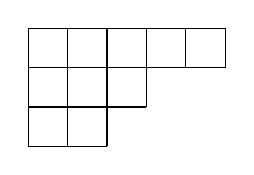
\begin{tikzpicture}
        \begin{scope}[scale=0.5]
            \draw (0, 3) -- (5, 3); \draw (0, 2) -- (5, 2); \draw (0, 1) -- (3, 1); \draw (0, 0) -- (2, 0); \draw (0, 3) -- (0, 0); \draw (1, 3) -- (1, 0); \draw (2, 3) -- (2, 0); \draw (3, 3) -- (3, 1); \draw (4, 3) -- (4, 2); \draw (5, 3) -- (5, 2);
        \end{scope}
    \end{tikzpicture} \]
    The \textit{arm length} of a box $s$, denoted $a_\lambda(s)$, is the number of boxes to the right of $s$. The \textit{leg length} of $s$, denoted $l_\lambda(s)$, is the number of boxes below $s$.
    
    A \textbf{Young tableau} is obtained from a Young diagram by filling in the boxes with numbers. A Young tableau is \textbf{standard} if the entries in each row and each column are increasing.
\end{topic}

\begin{topic}{generating-function}{generating function}
    The \textbf{generating function} of a sequence $a_0, a_1, a_2, \ldots$ in a \tref{AA:ring}{commutative ring} $R$ is the formal power series
    \[ \sum_{n = 0}^{\infty} a_n t^n = a_0 + a_1 t + a_2 t^2 + \cdots \in R \llbracket t \rrbracket . \]
\end{topic}

\begin{example}{generating-function}
    \begin{itemize}
        \item The generating function of the constant sequence $1, 1, 1, \ldots$ is
        \[ \sum_{n = 0}^{\infty} t^n = \frac{1}{1 - t} . \]
        \item The generating function of the linear sequence $0, 1, 2, 3, \ldots$ is
        \[ \sum_{n = 0}^{\infty} n t^{n} = t \cdot \frac{d}{dt} \sum_{n = 0}^{\infty} t^{n} = t \cdot \frac{d}{dt} \left( \frac{1}{1 - t} \right) = \frac{t}{(1 - t)^2} . \]
        % \item The generating function of 
    \end{itemize}
\end{example}

\begin{example}{generating-function}
    Assuming $R$ has \tref{AA:characteristic}{characteristic} zero, the sequence can be obtained from the generating function $F \in R \llbracket t \rrbracket$ as follows. Writing
    \[ F = \sum_{n = 0}^{\infty} a_n t^n = a_0 + a_1 t + a_2 t^2 + \cdots , \]
    we obtain the coefficients $a_n$ from the $n$-th derivatives of $F$ as
    \[ a_n = \frac{F^{(n)}(0)}{n!} . \]
\end{example}

\begin{topic}{mobius-function}{Möbius function}
    The \textbf{Möbius function} $\mu$ is the function that assigns to any positive integer $n > 0$ the value
    \[ \mu(n) = \sum_{\substack{1 \le k \le n \\ \gcd(k, n) = 1}} e^{2\pi i \frac{k}{n}} , \]
    or alternatively,
    \[ \mu(n) = \left\{ \begin{array}{cl}
         +1 & \textup{ if $n$ is square-free with even number of prime factors}, \\
         -1 & \textup{ if $n$ is square-free with odd number of prime factors}, \\
         0 & \textup{ if $n$ has a squared prime factor}.
    \end{array} \right. \]
\end{topic}

\begin{example}{mobius-function}
    The first few values of $\mu$ are given by
    \[ \begin{array}{lllll}
        \mu(1) = 1, & \mu(2) = -1, & \mu(3) = -1, & \mu(4) = 0, & \mu(5) = -1, \\
        \mu(6) = 1, & \mu(7) = -1, & \mu(8) = 0, & \mu(9) = 0, & \mu(10) = 1, \ldots
    \end{array} \]
\end{example}

\begin{topic}{cantor-theorem}{Cantor's theorem}
    \textbf{Cantor's theorem} states that the cardinality of a set $A$ is always strictly smaller than the cardinality of its power set $\mathcal{P}(A)$.
\end{topic}

\begin{example}{cantor-theorem}
    \begin{proof}
        The cardinality of $A$ is at most the cardinality of $\mathcal{P}(A)$ since $x \mapsto \{ x \}$ is an injection $A \to \mathcal{P}(A)$.
        Conversely, suppose that there exists a surjective function $f : A \to \mathcal{P}(A)$, and let $B = \{ x \in A \;|\; x \not\in f(x) \}$. Then by surjectivity of $f$ there exists some $y \in A$ such that $f(y) = B$. But then $y \in B$ if and only if $y \not\in f(y) = B$, which is a contradiction. Therefore, the cardinality of $A$ is strictly smaller than that of $\mathcal{P}(A)$.
    \end{proof}
\end{example}

\begin{topic}{schur-function}{Schur function}
    Let $n$ be a positive integer. Write $a_\alpha = \det(x_i^{\alpha_j})_{i, j = 1}^{n}$ for any sequence $\alpha = (\alpha_1, \ldots, \alpha_n)$. For any partition $\lambda = (\lambda_1, \ldots, \lambda_n)$ of length at most $n$, the \textbf{Schur polynomial} of $\lambda$ is the \tref{AA:symmetric-polynomial}{polynomial}
    \[ s_\lambda = a_{\lambda + \delta} / a_\delta \in \ZZ[x_1, \ldots, x_n] , \]
    where $\delta = (n - 1, n - 2, \ldots, 1, 0)$.
    
    In passing from $n$ to $n + 1$, it can be seen that $s_\lambda(x_1, x_2, \ldots, x_n, 0) = s_\lambda(x_1, x_2, \ldots, x_n)$. Hence, there is a uniquely defined element
    \[ s_\lambda \in \Lambda := \bigoplus_{r \ge 0} \Lambda^r , \quad \textup{ where  } \Lambda^r = \varprojlim_n \ZZ[x_1, \ldots, x_n]_{(r)}^{S_n} , \]
    called the \textbf{Schur function} of $\lambda$.
\end{topic}

\begin{example}{schur-function}
    For $n = 3$, we have
    \begin{itemize}
        \item $s_{(0, 0, 0)} = 1$,
        \item $s_{(1, 0, 0)} = x_1 + x_2 + x_3$,
        \item $s_{(1, 1, 0)} = x_1 x_2 + x_1 x_3 + x_2 x_3$,
        \item $s_{(1, 1, 1)} = x_1 x_2 x_3$,
        \item $s_{(2, 0, 0)} = x_1^2 + x_1 x_2 + x_1 x_3 + x_2^2 + x_2 x_3 + x_3^2$,
        \item $s_{(2, 1, 0)} = (x_1 + x_2) (x_1 + x_3) (x_2 + x_3)$.
    \end{itemize}
    For any $n \ge 1$ and $\lambda = (1, 0, 0, \ldots)$, we have $s_\lambda = \sum_{i = 1}^{n} x_i$, so we obtain the Schur function $s_\lambda = \sum_{i = 1}^{\infty} x_i \in \Lambda$.
\end{example}

% \begin{topic}{macdonald-polynomials}{Macdonald polynomials}
%     Let $q$ and $t$ be two parameters.
    
%     The \textbf{Macdonald polynomials} are a family of polynomials $P_\lambda(q, t)$ uniquely determined by the conditions
%     \[ P_\lambda(q, t) = m_\lambda + \sum_{\mu < \lambda} m_\mu \]
%     \[ \langle P_\lambda, P_\mu \rangle_{q, t} = 0 \quad \textup{ for } \lambda \ne \mu . \]
%     where
%     \[ \langle p_\lambda, p_\mu \rangle = \delta_{\lambda \mu} z_\lambda \prod_{i = 1}^{\ell(\lambda)} \frac{1 - q^{\lambda_i}}{1 - t^{\lambda_i}} . \]
% \end{topic}


\chapter{Set Theory}
\renewcommand{\cat}{ST}
\begin{topic}{power-set}{power set}
    The \textbf{power set} of a set $A$ is the set of all subsets of $A$,
    \[ P(A) = \{ B \mid B \subset A \} . \]
\end{topic}

\begin{topic}{cantor-theorem}{Cantor's theorem}
    \textbf{Cantor's theorem} states that for any set $A$, there does not exist a surjective function from $A$ to the \tref{power-set}{power set} $P(A)$ of $A$.
\end{topic}

\begin{example}{cantor-theorem}
    \begin{proof}
        Suppose for a contradiction that $f : A \to P(A)$ is a surjective function, and let $S = \{ x \in A \mid x \not\in f(x) \}$. Since $f$ is surjective, there exists some $x \in A$ with $f(x) = S$. But now, by definition of $S$,
        \[ x \in S \iff x \not\in f(x) = S , \]
        which is a contradiction.
    \end{proof}
\end{example}

\begin{topic}{axiom-of-choice}{axiom of choice}
    The \textbf{axiom of choice} states that for every set $X$ of non-empty sets, there exists a function
    \[ f : X \to \bigcup_{A \in X} A \]
    such that $f(A) \in A$ for all $A \in X$.
\end{topic}

\begin{topic}{cantor-set}{Cantor set}
    The \textbf{Cantor set} is the set
    \[ C = \bigcap_{n = 0}^{\infty} C_n , \]
    where $C_0 = [0, 1]$ and $C_n = \frac{1}{3} \left( C_{n - 1} \cup (2 + C_{n - 1}) \right)$ for any $n \ge 1$.
\end{topic}

\begin{topic}{partition}{partition}
    A \textbf{partition} of a set $X$ is a set $P$ of subsets of $X$ such that $\bigcup_{A \in P} A = X$ and $A \cap B = \varnothing$ for distinct $A, B \in P$.
\end{topic}

\begin{topic}{partially-ordered-set}{partially ordered set}
    A \textbf{partial order} on a set $P$ is a \tref{binary-relation}{binary relation} $\le$ on $P$ such that
    \begin{itemize}
        \item (\textit{reflexivity}) $x \le x$ for all $x \in P$,
        \item (\textit{anti-symmetry}) if $x \le y$ and $y \le x$ then $x = y$ for all $x, y \in P$,
        \item (\textit{transitivity}) if $x \le y$ and $y \le z$ then $x \le z$ for all $x, y, z \in P$.
    \end{itemize}
    A \textbf{partially ordered set} is a set $P$ together with a partial order $\le$.
\end{topic}

\begin{topic}{lattice}{lattice}
    A \textbf{lattice} is a \tref{partially-ordered-set}{partially ordered set} $(P, \le)$ such that
    \begin{itemize}
        \item (\textit{least upper bound}) any two elements $x, y \in P$ have a least upper bound $x \vee y$,
        \item (\textit{greatest lower bound}) any two elements $x, y \in P$ have a greatest lower bound $x \wedge y$,
        \item (\textit{least element}) there exists a least element $0 \in P$,
        \item (\textit{greatest element}) there exists a greatest element $1 \in P$.
    \end{itemize}
\end{topic}

\begin{topic}{boolean-algebra}{Boolean algebra}
    A \textbf{Boolean algebra} is a \tref{lattice}{lattice} $(P, \le)$ such that
    \begin{itemize}
        \item (\textit{complements}) for every $x \in P$ there exists an element $\neg x \in P$ such that $x \vee \neg x = 1$ and $x \wedge \neg x = 0$,
        \item (\textit{distributivity}) $x \wedge (y \vee z) = (x \wedge y) \vee (x \wedge z)$ for all $x, y, z \in P$.
    \end{itemize}
    A Boolean algebra $(P, \le)$ is \textbf{complete} if every subset $A \subset P$ has a least upper bound and a greatest lower bound.
\end{topic}

\begin{example}{boolean-algebra}
    Let $X$ be a set, and let $P$ be the \tref{power-set}{power set} of $X$. Then $(P, \subset)$ is a Boolean algebra, where the negation $\neg A$ is the difference $X \setminus A$.
\end{example}

\begin{topic}{atom}{atom}
    Let $(P, \le)$ be a \tref{partially-ordered-set}{partially ordered set} with a least element $0 \in P$. An \textbf{atom} in $P$ is an element $x \in P$ not equal to $0$ such that $y \le x$ implies $y = 0$ or $y = x$ for all $y \in P$.
\end{topic}

\begin{topic}{heyting-algebra}{Heyting algebra}
    A \textbf{Heyting algebra} is a \tref{lattice}{lattice} $(H, \le, \vee, \wedge, 0, 1)$ together with a binary operation $\rightarrow$, called \textit{Heyting implication}, such that $x \wedge y \le z$ if and only if $x \le y \rightarrow z$ for all $x, y, z \in H$.
\end{topic}

\begin{topic}{binary-relation}{binary relation}
    A \textbf{binary relation} $R$ over two sets $X$ and $Y$ is a subset of the product $X \times Y$.
    
    Usually, one writes $x R y$ to mean $(x, y) \in R$.
\end{topic}

\begin{topic}{filter}{filter}
    Let $(P, \le)$ be a \tref{partially-ordered-set}{partially ordered set}. A \textbf{filter} on $P$ is a subset $F \subset P$ such that
    \begin{itemize}
        \item (\textit{non-empty}) $F$ is non-empty,
        \item (\textit{downward directed}) for every $x, y \in F$ there exists some $z \in F$ with $z \le x$ and $z \le y$,
        \item (\textit{upward-closed}) for all $x \in F$ and $y \in P$ with $x \le y$, also $y \in F$.
    \end{itemize}
\end{topic}

\begin{example}{filter}
    Let $X$ be a \tref{TO:topological-space}{topological space}, and $x \in X$ a point. The \textit{neighborhood filter} of $x$, denoted $\mathcal{N}_x$, is the filter consisting of all \tref{TO:neighborhood}{neighborhoods} of $x$. It is a filter on the set of all subsets of $X$, partially ordered by inclusion.
\end{example}

\begin{topic}{de-morgan-laws}{De Morgan's laws}
    Let $B$ be a \tref{boolean-algebra}{Boolean algebra}. \textbf{De Morgan's laws} state that
    \[ \neg (x \lor y) = \neg x \land \neg y \quad \textup{ and } \quad \neg (x \land y) = \neg x \lor \neg y \]
    for all $x, y \in B$.
\end{topic}

\begin{topic}{modular-lattice}{modular lattice}
    A \tref{lattice}{lattice} $(P, \le)$ is \textbf{modular} if
    \[ x \lor (y \land z) = (x \lor y) \land z \]
    for all $x, y, z \in P$ with $x \le z$.
\end{topic}

\begin{example}{modular-lattice}
    Let $R$ be a \tref{AA:ring}{ring} and $M$ an \tref{AA:module}{$R$-module}. Then the lattice of submodules of $M$ with respect to inclusions, sums and intersections, is a modular lattice. That is, for any submodules $A, B, C \subset M$ with $A \subset C$, we have
    \[ A + (B \cap C) = (A + B) \cap C . \]
    Indeed, for any $x \in A + (B \cap C)$, we can write $x = a + y$ with $a \in A$ and $y \in B \cap C$. Since $A \subset C$, we have $a \in A \cap C$, so $x \in (A + B) \cap C$. Conversely, for any $x \in (A + B) \cap C$, we can write $x = a + b$ with $a \in A$ and $b \in B$ and $a + b \in C$. Since $a \in A \subset C$, also $b = (a + b) - a \in C$, so $x \in A + (B \cap C)$.
\end{example}


\chapter{Logic}
\renewcommand{\cat}{LO}
\begin{topic}{diaconescu-theorem}{Diaconescu's theorem}
    \textbf{Diaconescu's theorem} states that the \tref{ST:axiom-of-choice}{axiom of choice} implies the law of the excluded middle.
\end{topic}

\begin{example}{diaconescu-theorem}
    \begin{proof}
        Let $P$ be any proposition. Define the sets
        \[ A = \{ x \in \{ 0, 1 \} \mid (x = 0) \lor P \} \quad \textup{ and } \quad B = \{ x \in \{ 0, 1 \} \mid (x = 1) \lor P \} . \]
        By the axiom of choice, there exists a function $f : \{ A, B \} \to A \cup B$ such that $f(A) \in A$ and $f(B) \in B$. By definition of $A$ and $B$, this means that
        \[ (f(A) = 0) \lor P \quad \textup{ and } \quad (f(B) = 1) \lor P , \]
        which is equivalent to
        \[ (f(A) \ne f(B)) \lor P . \]
        Now, since $P \Rightarrow (A = B) \Rightarrow (f(A) = f(B))$, it follows that $(f(A) \ne f(B)) \Rightarrow \neg P$, which shows that $\neg P \lor P$.
    \end{proof}
\end{example}


\chapter{Combinatorics}
\renewcommand{\cat}{CO}
\begin{topic}{graph}{graph}
    A \textbf{graph} consists of a set $V$ together with a set $E \subset \{ \{ x, y \} : x, y \in V \textup{ and } x \ne y \}$.
    
    A \textbf{directed graph} consists of a set $V$ together with a set $E \subset \{ (x, y) : x, y \in V \textup{ and } x \ne y \}$.
    
    The elements of $V$ are called \textit{vertices} and the elements of $E$ are called \textit{edges}.
\end{topic}

\begin{topic}{matroid}{matroid}
    A \textbf{(finite) matroid} is a finite set $E$, called the \textit{ground set}, together with a set $I$ of subsets of $E$, known as the \textit{independent subsets}, such that
    \begin{itemize}
        \item $\varnothing \in I$,
        \item if $B \in I$ and $A \subset B$, then $A \in I$,
        \item if $A, B \in I$ and $|B| > |A|$, then there exists an $b \in B$ such that $A \cup \{ b \} \in I$.
    \end{itemize}
\end{topic}

\begin{example}{matroid}
    \begin{itemize}
        \item Let $E$ be a \tref{LA:vector-space}{vector space}, and $I$ the set of \tref{LA:linearly-independent}{linearly independent} subsets of $E$. Then $(E, I)$ is a matroid.
        \item Let $G$ be a finite \tref{graph}{graph}, and $E$ its set of edges. Let $I$ be the set of subsets of edges that are a \textit{forest}, that is, subsets of edges that do not contain a cycle. Then $(E, I)$ is a matroid.
    \end{itemize}
\end{example}

\begin{topic}{tutte-polynomial}{Tutte polynomial}
    Let $G = (V, E)$ be a \tref{graph}{graph}. The \textbf{Tutte polynomial} of $G$ is the polynomial, in two variables $x$ and $y$, given by
    \[ T_G(x, y) = \sum_{E' \subset E} (x - 1)^{k(E') - k(E)} (y - 1)^{k(E') + |E'| - |V|} \]
    where $k(E')$ denotes the number of connected components of the graph $(V, E')$.
\end{topic}

\begin{topic}{quiver}{quiver}
    A \textbf{quiver} is a finite \tref{graph}{directed graph}, where loops and multiple arrows between vertices are allowed.
\end{topic}

\begin{topic}{quiver-representation}{quiver representation}
    Let $Q$ be a \tref{quiver}{quiver}. A \textbf{representation} of $Q$ is a collection of vector spaces $V_i$ for each vertex $i \in Q_0$ and linear maps $V(\alpha) \colon V_i \to V_j$ for each arrow $(\alpha \colon i \to j) \in Q_1$.
    
    A \textbf{morphism} of quiver representations $V \to W$ is a collection of maps $\varphi_i \colon V_i \to W_i$ for each vertex $i \in Q_0$ such that $\varphi_j V(\alpha) = W(\alpha) \varphi_i$.
    
    The sequence of dimensions $(\dim V_i)_{i \in Q_0} \in \NN^{Q_0}$ is called the \textbf{dimension vector}.
\end{topic}

\begin{topic}{path-algebra}{(quiver) path algebra}
    Let $Q$ be a \tref{quiver}{quiver}. A \textbf{path} in $Q$ is a sequence $\alpha_n \alpha_{n - 1} \cdots \alpha_1$ of arrows such that the head of $\alpha_{i + 1}$ equals the tail of $\alpha_{i}$. The \textbf{path algebra} of $Q$ is defined as a \tref{LA:vector-space}{vector space} with the set of paths of $Q$ as a basis. Multiplication is given by concatenation of paths, and if two paths cannot be connected because their endpoints are different, their product is defined as zero.
\end{topic}

\begin{topic}{euler-form}{Euler form}
    Let $Q$ be a \tref{quiver}{quiver}. The \textbf{Euler form} of $Q$ is the bilinear form on $\ZZ^{Q_0}$ given by
    \[ \langle d, e \rangle_Q = \sum_{i \in Q_0} d_i e_i - \sum_{(\alpha \colon i \to j) \in Q_1} d_i e_j \]
    for any $d = (d_i)_{i \in Q_0}$ and $e = (e_i)_{i \in Q_0}$.
\end{topic}

\begin{topic}{tits-form}{Tits form}
    Let $Q$ be a \tref{quiver}{quiver}. The \textbf{Tits form} of $Q$ is the quadratic form on $\ZZ^{Q_0}$ given by
    \[ q_Q(d) = \langle d, d \rangle_Q = \sum_{i \in Q_0} d_i^2 - \sum_{(\alpha \colon i \to j) \in Q_1} d_i d_j \]
    for any $d = (d_i)_{i \in Q_0}$, where $\langle \cdot, \cdot \rangle_Q$ denotes the \tref{euler-form}{Euler form} of $Q$.
\end{topic}


\chapter{Linear Algebra}
\renewcommand{\cat}{LA}
\begin{topic}{vector-space}{vector space}
    A \textbf{vector space} over a \tref{CA:field}{field} $k$ is a $k$-module. Its elements are called \textit{vectors}.
    % Concretely, ...
\end{topic}

\begin{topic}{vector-subspace}{vector-subspace}
    Let $V$ be a \tref{vector-space}{vector space}. A \textbf{subspace} of $V$ is a subset $V' \subset V$ which is a vector space itself.
\end{topic}

\begin{topic}{linearly-independent}{linearly independent}
    Let $V$ be a \tref{vector-space}{vector space}. A set of vectors $S \subset V$ is said to be \textbf{linearly independent} if for any relation
    \[ \sum_{i = 1}^{n} a_i v_i = 0, \qquad \text{with $v_i \in S$ and $a_i \in k$,} \]
    one has $a_i = 0$.
\end{topic}

\begin{topic}{span}{span}
    Let $V$ be a \tref{vector-space}{vector space}, and $S \subset V$ a subset. The \textbf{span} of $S$ is the subspace of all linear combinations of vectors in $S$.
    \[ \text{span}(S) = \left\{ \sum_{i = 1}^{n} a_i v_i \text{ for any } v_i \in S \text{ and } a_i \in k \right\} \]
\end{topic}

\begin{topic}{basis}{basis}
    Let $V$ be a \tref{vector-space}{vector space}. A set of vectors in $V$ is a \textbf{basis} for $V$ if it \tref{span}{spans} $V$ and is \tref{linearly-independent}{linearly independent}.
    
    Equivalently, a set is a basis if each vector in $V$ can be expressed uniquely as a linear combination of vectors in the set.
\end{topic}

\begin{topic}{dimension}{dimension}
    Let $V$ be a \tref{vector-space}{vector space}. The \textbf{dimension} of $V$ is the cardinality of any basis of $V$. It is often denoted by $\dim(V)$.
\end{topic}

\begin{topic}{linear-transformation}{linear transformation}
    A function $T : V \to V$ is a \textbf{linear transformation} if
    \begin{itemize}
        \item $T(v + w) = T(v) + T(w)$,
        \item $T(av) = aT(v)$,
    \end{itemize}
    for all vectors $v, w \in V$ and scalars $a \in k$.
\end{topic}

\begin{topic}{matrix-representation}{matrix representation}
    Let $V$ and $W$ be finite-dimensional \tref{vector-space}{vector spaces}, and $T : V \to W$ a \tref{linear-transformation}{linear transformation}. If $(v_1, v_2, \ldots, v_n)$ and $(w_1, w_2, \ldots, w_m)$ are (ordered) \tref{basis}{bases} of $V$ and $W$, respectively, then the \textbf{matrix representation} of $T$ is the $m \times n$ matrix
    \[ A = \begin{pmatrix} a_{11} & a_{21} & \cdots & a_{n1} \\ a_{21} & a_{22} & \cdots & a_{2n} \\ \vdots & \vdots & \ddots & \vdots \\ a_{m1} & a_{m2} & \cdots & a_{mn} \end{pmatrix} \]
    such that $i$-th component of $T(v_j)$ (w.r.t. the basis for $W$) is $a_{ij}$.
\end{topic}

\begin{topic}{matrix-multiplication}{matrix multiplication}
    Let $A = (a_{ij})$ be an $m \times n$ matrix, and $B = (b_{ij})$ be an $n \times \ell$ matrix. The \textbf{matrix product} $AB$ is the $m \times \ell$ matrix $C = (c_{ij})$ given by
    \[  c_{ij} = \sum_{k = 1}^{n} a_{ik} b_{kj} . \]
\end{topic}

\begin{topic}{matrix-transpose}{matrix transpose}
    The \textbf{transpose} of a matrix $A = (a_{ij})$ is the matrix $A^T = (b_{ij})$ given by $b_{ij} = a_{ji}$.
\end{topic}

% \begin{topic}{row-echelon-form}{(reduced) row-echelon form}
    
% \end{topic}

\begin{topic}{invertible-matrix}{invertible matrix}
    An $n \times n$ matrix $A$ is \textbf{invertible} if there exists an $n \times n$ matrix $B$ such that $AB = BA = I$. In this case, $B$ is called the \textbf{inverse} of $A$, and is the unique matrix with this property.
    
    If $A$ is not invertible, it is called \textbf{singular}.
\end{topic}

\begin{topic}{matrix-rank}{matrix rank}
    The \textbf{rank} of an $m \times n$ matrix $A$ the \tref{dimension}{dimension} of its \textit{row space} $\im A$.
\end{topic}

\begin{topic}{nullspace}{nullspace}
    The \textbf{nullspace}, or \textbf{kernel}, of a \tref{linear-transformation}{linear transformation} $T : V \to W$ is the subspace
    \[ \left\{ v \in V \text{ such that } T(v) = 0 \right\} \subset V . \]
\end{topic}

\begin{topic}{projection}{projection}
    A \textbf{projection} is a \tref{linear-transformation}{linear transformation} $P : V \to V$ with $P^2 = P$.
\end{topic}

\begin{topic}{determinant}{determinant}
    The \textbf{determinant} of an $n \times n$ matrix $A$ is the scalar given by
    \[ \det(A) = \sum_{\sigma \in S_n} \left( \text{sign}(\sigma) \prod_{i = 1}^{n} a_{i, \sigma(i)} \right) . \]
    It has the property that $A$ is \tref{invertible-matrix}{invertible} if and only if $\det(A) \ne 0$.
    
    Also, the determinant of $A$ is the scalar corresponding to the map induced on the top exterior power of $V$,
    \[ \wedge^n A : \wedge^n V \to \wedge^n V . \]
\end{topic}

\begin{topic}{cofactor-matrix}{cofactor matrix}
    Let $A = (a_{ij})$ be an $n \times n$ matrix. The \textbf{cofactor} of an entry $a_{ij}$ of $A$ is
    \[ a'_{ij} = (-1)^{i + j} \det(A_{ij}), \]
    where $A_{ij}$ is the matrix obtained from $A$ by removing the $i$-th row and $j$-th column. The \textbf{cofactor matrix} of $A$ is then the $n \times n$ matrix $A' = (a'_{ij})$.
\end{topic}

\begin{topic}{adjoint-matrix}{adjoint matrix}
    Let $A$ be an $n \times n$ matrix. The \textbf{adjoint} of $A$ is the \tref{matrix-transpose}{transpose} of its \tref{cofactor-matrix}{cofactor matrix}:
    \[ \text{adj}(A) = (A')^T . \]
    It has the property that
    \[ \text{adj}(A) A = \det(A) I , \]
    so in particular, when $\det(A) \ne 0$, one has
    \[ A^{-1} = \frac{1}{\det(A)} \text{adj}(A) . \]
\end{topic}

\begin{topic}{eigenvalue}{eigenvalue/eigenvector}
    Let $A$ be an $n \times n$ matrix. A scalar $\lambda$ is an \textbf{eigenvalue} of $A$ if there exists a nonzero vector $v$ such that $A v = \lambda v$. The vector $v$ is then an \textbf{eigenvector} of $A$ corresponding to $\lambda$.
\end{topic}

\begin{topic}{characteristic-polynomial}{characteristic polynomial}
    Let $A$ be an $n \times n$ matrix. The \textbf{characteristic polynomial} of $A$ is the polynomial of degree $n$ given by
    \[ p_A(\lambda) = \det(A - \lambda I) . \]
    Its roots are precisely the \tref{eigenvalue}{eigenvalues} of $A$.
\end{topic}

\begin{topic}{diagonalization}{diagonalization}
    A \textbf{diagonalization} of an $n \times n$ matrix $A$ consists of an invertible matrix $C$ and a diagonal matrix $D$ such that
    \[ D = C A C^{-1} . \]
    If such a diagonalization exists, $A$ is said to be \textbf{diagonalizable}.
\end{topic}

\begin{topic}{algebraic-geometric-multiplicity}{algebraic/geometric multiplicity}
    Let $A$ be an $n \times n$ matrix. The \textbf{algebraic multiplicity} of an eigenvalue $\lambda$ of $A$ is its multiplicity as a root of the \tref{characteristic-polynomial}{characteristic polynomial} of $A$.
    
    The \textbf{geometric multiplicity} is the \tref{dimension}{dimension} of the corresponding \textit{eigenspace}
    \[ E_\lambda = \{ v \in V : A v = \lambda v \} . \]
\end{topic}

\begin{example}{algebraic-geometric-multiplicity}
    Consider the matrix
    \[ A = \begin{pmatrix} 2 & 1 & 0 \\ 0 & 2 & 0 \\ 0 & 0 & 3 \end{pmatrix} . \]
    Its characteristic polynomial is $p_A(\lambda) = (2 - \lambda)^2 (3 - \lambda)$. Hence the eigenvalues are $\lambda = 2$ (with alg. multiplicity $2$) and $\lambda = 3$ (with alg. multiplicity $1$). However, both have a geometric multiplicity of $1$ as
    \[ E_2 = \ker(A - 2I) = \text{span}(1, 0, 0) \quad \text{ and } \quad E_3 = \ker(A - 3I) = \text{span}(0, 0, 1) . \]
\end{example}

\begin{topic}{symplectic-vector-space}{symplectic vector space}
    A \textbf{symplectic vector space} is a real \tref{vector-space}{vector space} together with a skew-symmetric non-degenerate bilinear map $\omega : V \times V \to \RR$, called the \textbf{symplectic form}.
\end{topic}

\begin{topic}{symplectic-complement}{symplectic complement}
    Let $(V, \omega)$ be a \tref{symplectic-vector-space}{symplectic vector space}, and $W \subset V$ a linear subspace. The \textbf{symplectic complement} of $W$ is the subspace
    \[ W^\perp = \{ v \in V : \omega(v, w) = 0 \text{ for all } w \in W \} . \]
\end{topic}

\begin{topic}{symplectic-subspace}{symplectic subspace}
    A \textbf{symplectic subspace} of a \tref{symplectic-vector-space}{symplectic vector space} $(V, \omega)$ is a linear subspace $W \subset V$ satisfying $W \cap W^\perp = \{ 0 \}$.
    
    This is the case if and only if $\omega$ restricts to a symplectic form on $W$.
\end{topic}

\begin{topic}{isotropic-subspace}{(co)isotropic subspace}
    Let $(V, \omega)$ be a \tref{symplectic-vector-space}{symplectic vector space}. A linear subspace $W \subset V$ is \textbf{isotropic} if $W \subset W^\perp$, and \textbf{coisotropic} if $W^\perp \subset W$.
    
    Equivalently, $W$ is \textbf{isotropic} if and only if $\omega|_W = 0$. And $W$ is \textbf{coisotropic} if and only if $\omega$ restricts to a symplectic form on $W/W^\perp$.
\end{topic}

\begin{topic}{lagrangian-subspace}{Lagrangian subspace}
    Let $(V, \omega)$ be a \tref{symplectic-vector-space}{symplectic vector space}. A linear subspace $W \subset V$ is \textbf{Lagrangian} if $W = W^\perp$.
\end{topic}

\begin{topic}{polyhedral-cone}{polyhedral cone}
    A \textbf{polyhedral cone} in $\RR^n$ is a set of the form
    \[ \sigma = \{ \lambda_1 v_1 + \cdots + \lambda_r v_r : \lambda_i \in \RR \} , \]
    for some $v_1, \ldots, v_r \in \RR^n$. The vectors $v_1, \ldots, v_r$ are called \textit{generators} of the cone $\sigma$.
    
    The \textit{dimension} of $\sigma$ is the dimension of the linear subspace spanned by $\sigma$.
\end{topic}

\begin{topic}{dual-cone}{dual cone}
    The \textbf{dual cone} of a \tref{polyhedral-cone}{polyhedral cone} $\sigma \subset \RR^n$ is
    \[ \sigma^\vee = \{ u \in (\RR^n)^* : \langle u, v \rangle \ge 0 \text{ for all } v \in \sigma \} . \]
\end{topic}

\begin{topic}{minkowski-theorem}{Minkowski's theorem}
    Let $L$ be a lattice in $\RR^n$, and $S \subset \RR^n$ a convex subset, which is symmetric with respect to the origin. That is, for all $x \in S$ also $-x \in S$. Then \textbf{Minkowski's theorem} states that if the volume of $S$ is strictly larger than $2^n \det(L)$, then $S$ must contain at least one non-zero lattice point of $L$.
\end{topic}

\begin{example}{minkowski-theorem}
    The given bound is sharp. Namely, consider $L = \ZZ^n$ with $\det(L) = 1$, and $S$ the interior of $[-1, 1]^n$, whose volume is $2^n$. Then $S$ does not contain any non-zero lattice points.
\end{example}

\begin{example}{minkowski-theorem}
    \begin{proof}
        By assumption, the set $\tfrac{1}{2} S = \{ \tfrac{1}{2} x : x \in S \}$ has volume $\textup{vol}(\tfrac{1}{2} S) = 2^{-n} \textup{vol}(S) > \textup{vol}(\RR^n/L)$, so the map $\tfrac{1}{2} S \to \RR^n / L$ cannot be injective. Hence, there are distinct points $x_1, x_2 \in S$ such that $\tfrac{1}{2} x_1 - \tfrac{1}{2} x_2 \in L$. Since $-x_2 \in S$ and $S$ is convex, the linear combination $\tfrac{1}{2} x_1 - \tfrac{1}{2} x_2$ is a non-zero lattice point in $S$.
    \end{proof}
\end{example}

\begin{topic}{root-system}{root system}
    Let $V$ be a finite-dimensional real or complex \tref{vector-space}{vector space} with an \tref{FA:inner-product}{inner product} $(\cdot, \cdot)$. A \textbf{root system} $\Phi$ in $V$ is a finite set of non-zero vectors in $V$, called \textbf{roots}, such that
    \begin{itemize}
        \item (\textit{span}) $\Phi$ spans $V$,
        \item (\textit{multiples}) if $\alpha \in \Phi$, then $n \alpha \in \Phi \iff n = \pm 1$,
        \item (\textit{reflection}) $\beta - \frac{2 (\alpha, \beta)}{(\alpha, \alpha)} \alpha \in \Phi$ for all $\alpha, \beta \in \Phi$,
        \item (\textit{integrality}) $\frac{2 (\alpha, \beta)}{\alpha, \alpha}$ is an integer for all $\alpha, \beta \in \Phi$.
    \end{itemize}
    Given a root system $\Phi$, one can always choose (non-uniquely) a subset $\Phi^+ \subset \Phi$ such that
    \begin{itemize}
        \item for all $\alpha \in \Phi$, either $\alpha \in \Phi^+$ or $-\alpha \in \Phi^+$, but not both,
        \item for distinct $\alpha, \beta \in \Phi^+$ such that $\alpha + \beta \in \Phi$, also $\alpha + \beta \in \Phi^+$.
    \end{itemize}
    Roots in $\Phi^+$ are called \textbf{positive} and roots in $-\Phi^+$ are called \textbf{negative}. An root in $\Phi^+$ is called \textbf{simple} if it cannot be written as the sum of two positive roots. The set $\Pi$ of simple roots has the property that every $\alpha \in \Phi$ is a linear combination of elements of $\Pi$ with integer coefficients, which are either all positive or all negative.
\end{topic}

\begin{example}{root-system}
    Given a complex \tref{AA:semisimple-lie-algebra}{semisimple Lie algebra} $\mathfrak{g}$ and a \tref{AA:cartan-subalgebra}{Cartan subalgebra} $\mathfrak{h} \subset \mathfrak{g}$, one can construct a root system $\Phi$ in $\mathfrak{h}^*$, where a root is an element $\alpha \in \mathfrak{h}^*$ such that
    \[ \mathfrak{g}_\alpha = \{ x \in \mathfrak{g} : [h, x] = \alpha(h) x \textup{ for all } h \in \mathfrak{h} \} \]
    is non-empty.
\end{example}

\begin{topic}{pure-hodge-structure}{pure Hodge structure}
    A \textbf{pure Hodge structure of weight $k \in \ZZ$} consists of a $\ZZ$-module $H_\ZZ$ of finite rank, and a direct sum decomposition of the complexification
    \[ H_\CC := H_\ZZ \otimes_\ZZ \CC = \bigoplus_{p + q = k} H^{p, q} \quad \text{ with } \quad H^{p, q} = \overline{H^{q, p}} . \]
    One speaks of \textit{rational} or \textit{real} Hodge structures when replacing $H_\ZZ$ by a rational or real vector space.
    
    A \textbf{morphism of pure Hodge structures} is a morphism $f : H_\ZZ \to H'_\ZZ$ of $\ZZ$-modules such that its complexification $f_\CC$ preserves type, i.e. $f_\CC\left(H^{p, q}\right) \subset (H')^{p, q}$.
    
    The numbers $h^{p, q}(H) := \dim_\CC H^{p, q}$ are called the \textbf{Hodge numbers} of the Hodge structure.
\end{topic}

\begin{example}{pure-hodge-structure}
    For any $H_\ZZ$, taking $H^{k,k} = H_\CC$ and $H^{p, q} = 0$ when $(p, q) \ne (k, k)$ gives the \textit{trivial Hodge structure} of weight $2k$.
\end{example}

\begin{example}{pure-hodge-structure}
    Take $H_\ZZ = 2 \pi i \ZZ \subset \CC$ and $H_\CC = H^{-1, -1}$. This is a pure Hodge structure of weight $-2$. In fact, is the unique $1$-dimensional pure Hodge structure of weight $-2$ up to isomorphism, and it is called the \textit{Tate Hodge structure}, often denoted by $\ZZ(1)$.
\end{example}

\begin{topic}{hodge-filtration}{Hodge filtration}
    A \textbf{Hodge filtration} is an equivalent description of a \tref{pure-hodge-structure}{pure Hodge structure} of weight $k \in \ZZ$, given by a filtration
    \[ H_\CC \supset \cdots \supset F^p \supset F^{p + 1} \supset \cdots \quad \text{ with } \quad F^p \oplus \overline{F^q} = H_\CC \text{ for } p + q = k + 1 . \]
    A Hodge filtration can be obtained from a pure Hodge structure, and vice versa, via
    \[ F^p = \bigoplus_{r \ge p} H^{r, k - r} \quad \text{and} \quad H^{p, q} = F^p \cap \overline{F^q} . \]
    % Indeed $F^p$ gives a filtration, and for $p + q = k + 1$ one finds
    % \[ F^p = \bigoplus_{r \ge p} V^{r, k - r} \qquad \text{and} \qquad \overline{F^q} = \bigoplus_{s \ge k - p + 1} \overline{V^{s, k - s}} = \bigoplus_{r \le p - 1} V^{r, k - r}, \]
    % from which follows that $F^p \oplus \overline{F^q} = V_\CC$.
    % In the other direction
    % \[ \bigoplus_{p + q = k} H^{p, q} = \bigoplus_{p + q = k} F^p \cap \overline{F^q} = H_\CC , \]
    % because any $v \in H_\CC$ lies in $F^p \setminus F^{p + 1}$ for some unique $p$, and since $F^{p + 1} \oplus \overline{F^{k - p}} = H_\CC$, we have $v \in F^p \cap \overline{F^{k - p}}$. It is clear that $\overline{H^{p, q}} = H^{q, p}$.
\end{topic}

\begin{topic}{hodge-polynomial}{(mixed) Hodge polynomial}
    The \textbf{Hodge polynomial} of a \tref{pure-hodge-structure}{pure Hodge structure} $H$ is the polynomial,
    \[ P_\textup{hodge}(H) = \sum_{p, q \in \ZZ} h^{p, q}(H) u^p v^q , \]
    where $h^{p, q}(H) = \dim_\CC H^{p, q}$ denote the hodge numbers.
\end{topic}

\begin{topic}{mixed-hodge-structure}{mixed Hodge structure}
    A \textbf{mixed Hodge structure} on a $\ZZ$-module $H_\ZZ$ consists of an increasing $\ZZ$-filtration $W_\bdot$ on $H_\QQ = H_\ZZ \otimes \QQ$,
    \[ 0 \subset \cdots \subset W_i \subset W_{i + 1} \cdots \subset H_\QQ \]
    and a decreasing $\NN$-filtration $F^\bullet$ on $H_\CC = H_\ZZ \otimes \CC$,
    \[ H_\CC = F^0 \supset F^1 \supset \cdots \supset 0 \]
    such that the induced filtrations (obtained by intersections) of $F^\bdot$ on the graded pieces $\left(\text{Gr}^W_k H_\QQ\right) \otimes_\QQ \CC := \left(W_k H_\QQ / W_{k - 1} H_\QQ\right) \otimes_\QQ \CC$ are \tref{pure-hodge-structure}{pure (rational) Hodge structures} of weight $k$.
    
    A \textbf{morphism of mixed Hodge structures} is a morphism $f : H_\ZZ \to H'_\ZZ$ of $\ZZ$-modules compatible with the two filtrations $W_\bdot$ and $F^\bdot$.
    
    The numbers $h^{p, q}(H) := \dim_\CC \textup{Gr}_F^p \textup{Gr}^W_{p + q}(H_\CC)$ are called the \textbf{mixed Hodge numbers} of the mixed Hodge structure $H$.
\end{topic}

\begin{topic}{inner-product}{inner product}
    An \textbf{inner product} on a \tref{LA:vector-space}{vector space} $V$ over $k = \RR$ or $\CC$ is a map $\langle \cdot, \cdot \rangle \colon V \times V \to k$ satisfying
    \begin{itemize}
        \item (\textit{linearity}) $\langle \alpha x + \beta y, z \rangle = \alpha \langle x, z \rangle + \beta \langle y, z \rangle$ for all scalars $\alpha$ and $x, y, z \in V$,
        \item \textit{(conjugate symmetry)} $\langle x, y \rangle = \overline{\langle y, x \rangle}$ for all $x, y \in V$,
        \item (\textit{positive definiteness}) $\langle x, x \rangle > 0$ for all $x \ne 0$ in $V$.
    \end{itemize}
    A vector space together with an inner product is called an \textbf{inner product space}.
\end{topic}

\begin{topic}{cauchy-schwarz-inequality}{Cauchy--Schwarz inequality}
    The \textbf{Cauchy--Schwarz inequality} states that for any vectors $v, w$ in an \tref{inner-product}{inner-product-space},
    \[ \langle v, w \rangle^2 \le \langle v, v \rangle \cdot \langle w, w \rangle . \]
\end{topic}

\begin{topic}{polarization-identity}{polarization identity}
    Let $(V, \langle \cdot, \cdot \rangle)$ be an \tref{inner-product}{inner product space}. The polarization identity states that
    \[ \operatorname{Re} \langle x, y \rangle = \frac{1}{2} ( \norm{x + y} - \norm{x} - \norm{y} ) , \]
    where $\norm{x} = \langle x, x \rangle$.
\end{topic}


\chapter{Group Theory}
\renewcommand{\cat}{GT}
\begin{topic}{group}{group}
    A \textbf{group} is a set $G$ together with an operation $G \times G \to G$ (the \textit{group law}) written as $(x, y) \mapsto xy$, and an element $1 \in G$ (the \textit{unit}), satisfying
    \begin{itemize}
        \item (\textit{associativity}) $(xy)z = x(yz)$ for all $x, y, z \in G$,
        \item (\textit{unit element}) $1 \cdot x = x \cdot 1 = x$ for all $x \in G$,
        \item (\textit{inverses}) for all $x \in G$ there exists an $x^{-1} \in G$ such that $x x^{-1} = x^{-1} x = 1$, called the \textit{inverse} of $x$.
    \end{itemize}
\end{topic}

\begin{topic}{subgroup}{subgroup}
    A \textbf{subgroup} $H$ of a \tref{group}{group} $G$ is a subset $H \subset G$ which, with the same group law and unit, is itself a group.
\end{topic}

\begin{topic}{abelian-group}{abelian group}
    A \tref{group}{group} $G$ is called \textbf{abelian} if $xy = yx$ for all $x, y \in G$.
\end{topic}

\begin{topic}{order}{order}
    The \textbf{order} of a \tref{group}{group} $G$ is the number its elements.
    
    The \textbf{order} of an element $x \in G$, denoted $\text{ord}(x)$, is the least positive integer $n$ such that $x^n = 1$. If no such $n$ exists, then $\text{ord}(x) = \infty$.
\end{topic}

\begin{topic}{cyclic-group}{cyclic group}
    A \textbf{cyclic group} is a \tref{group}{group} $G$ generated by a single element $x \in G$, that is $G = \{ x^n : x \in \ZZ \}$.
\end{topic}

\begin{topic}{group-homomorphism}{group homomorphism}
    Let $G$ and $H$ be two \tref{group}{groups}. A \textbf{homomorphism} from $G$ to $H$ is a map $f : G \to H$ satisfying $f(xy) = f(x) f(y)$ for all $x, y \in G$.
\end{topic}

\begin{topic}{kernel}{kernel}
    Let $f : G \to H$ be a \tref{group-homomorphism}{group homomorphism}. The \textbf{kernel} of $f$, denoted $\ker f$, is defined as
    \[ \ker f = \{ x \in G : f(x) = 0 \} . \]
    It is a \tref{normal-subgroup}{normal} \tref{subgroup}{subgroup} of $G$.
\end{topic}

\begin{topic}{group-center}{group center}
    The \textbf{center} of a \tref{group}{group} $G$ is the subgroup
    \[ Z(G) = \{ x \in G : xy = yx \text{ for all } y \in G \} . \]
\end{topic}

\begin{topic}{symmetric-group}{symmetric group}
    Let $\Sigma$ be a set. The \textbf{symmetric group} on $\Sigma$ is the \tref{group}{group} $S_\Sigma$ of all bijections $\Sigma \to \Sigma$. The group law is given by composition, and the unit is the identity map.
    
    When $\Sigma = \{ 1, 2, \ldots, n \}$ for some integer $n \ge 1$, one writes $S_n$ for the symmetry group. Its elements are called \textbf{permutations}.
\end{topic}

\begin{topic}{cayleys-theorem}{Cayley's theorem}
    \textbf{Cayley's theorem} states that every \tref{group}{group} $G$ is isomorphic to a \tref{subgroup}{subgroup} of the \tref{symmetric-group}{symmetric group} $S_G$. In particular, $G$ is isomorphic to the image of the morphism
    \[ \varphi : G \to S_G, \qquad x \mapsto (y \mapsto xy) . \]
\end{topic}

\begin{topic}{cyclic-permutation}{cyclic permutation}
    A \tref{symmetric-group}{permutation} $\sigma \in S_n$ is a \textbf{cyclic permutation}, or \textbf{cycle}, of length $k$ if there exist $k$ distinct integers $1 \le a_1, \ldots, a_k \le n$ with $\sigma(a_i) = a_{i + 1}$ for $1 \le i < k$ and $\sigma(a_k) = a_1$, and $\sigma(x) = x$ for $x \not\in \{ a_1, \ldots, a_k \}$. This is denoted by
    \[ \sigma = (a_1 \;\; a_2 \;\; \ldots \;\; a_k) . \]
    A cycle of length $2$ is also called a \textbf{transposition}.
\end{topic}

\begin{topic}{permutation-sign}{permutation sign}
    The \textbf{sign} of a \tref{symmetric-group}{permutation} $\sigma \in S_n$ is defined as
    \[ \text{sign}(\sigma) = \prod_{1 \le i < j \le n} \frac{\sigma(j) - \sigma(i)}{j - i} \in \{ +1, -1 \} . \]
    We call $\sigma$ \textit{even} if $\text{sign}(\sigma) = 1$ and \textit{odd} if $\text{sign}(\sigma) = -1$.
    
    This defines a \tref{group-homomorphism}{group homomorphism}
    \[ \text{sign} : S_n \to \{ +1, -1 \} . \]
\end{topic}

\begin{topic}{alternating-group}{alternating group}
    For $n \ge 1$, the \textbf{alternating group} $A_n$ is the subgroup of the \tref{symmetric-group}{symmetric group} $S_n$ of all \tref{permutation-sign}{even} permutations.
\end{topic}

\begin{topic}{normal-subgroup}{normal subgroup}
    A \tref{subgroup}{subgroup} $N$ of a \tref{group}{group} $G$ is called \textbf{normal} if $N = g N g^{-1}$ for all $g \in G$.
\end{topic}

\begin{example}{normal-subgroup}
    The \tref{kernel}{kernel} of a morphism $f : G \to H$ is always a normal subgroup. Indeed, for any $x \in \ker f$ and $g \in G$ we have
    \[ f(gxg^{-1}) = f(g) f(x) f(g)^{-1} = f(g) f(g)^{-1} = 1 , \]
    so $gxg^{-1} \in \ker f$, and thus $g (\ker f) g^{-1} \subset \ker f$. The other inclusion is shown completely similarly.
    
    Conversely, any normal subgroup $N \subset G$ is the kernel of the quotient map $\pi : G \to G / N$.
\end{example}

\begin{topic}{central-subgroup}{central subgroup}
    A \tref{subgroup}{subgroup} $H$ of a \tref{group}{group} $G$ is called \textbf{central} if $H$ lies in the \tref{group-center}{center} of $G$.
\end{topic}

\begin{topic}{quotient-group}{quotient group}
    Let $G$ be a \tref{group}{group} and $N$ a \tref{normal-subgroup}{normal subgroup}. The \textbf{quotient group} $G/N$ is the group of cosets
    \[ G/N = \{ gN : g \in G \} \]
    with group law $(gN)(hN) = (gh)N$ and unit $N$.
\end{topic}

\begin{topic}{simple-group}{simple group}
    A \tref{group}{group} $G$ is called \textbf{simple} if its only \tref{normal-subgroup}{normal subgroups} are $\{ 1 \}$ and $G$.
\end{topic}

\begin{topic}{torsion-subgroup}{torsion subgroup}
    The \textbf{torsion subgroup} of a \tref{group}{group} $G$ is the subgroup of elements of finite \tref{order}{order}.
    \[ G_{\text{tor}} = \{ x \in G : \text{ord}(x) < \infty \} \]
\end{topic}

\begin{topic}{normalizer}{normalizer}
    Let $H$ be a \tref{subgroup}{subgroup} of a \tref{group}{group} $G$. The \textbf{normalizer} of $H$ is the subgroup
    \[ N_H = \{ x \in G : x H x^{-1} = H \} . \]
\end{topic}

\begin{topic}{group-action}{group action}
    Let $G$ be a \tref{group}{group} and $X$ a set. An \textbf{action} of $G$ on $X$ is map
    \[ G \times X \to X : (g, x) \mapsto g \cdot x \]
    satisfying $1 \cdot x = x$ and $g \cdot (h \cdot x) = (gh) \cdot x$ for all $g, h \in G$ and $x \in X$.
\end{topic}

\begin{topic}{centralizer}{centralizer}
    Let $G$ be a \tref{group}{group}. The \textbf{centralizer} of an element $g \in G$ is the subgroup
    \[ G_g = \{ h \in G : h x h^{-1} = g \} . \]
\end{topic}

\begin{topic}{stabilizer}{stabilizer}
    Let $G$ be a \tref{group}{group} \tref{group-action}{acting} on a set $X$. Then the \textbf{stabilizer} of $x \in X$ is the \tref{subgroup}{subgroup}
    \[ G_x = \{ g \in G : g \cdot x = x \} . \]
\end{topic}

\begin{topic}{orbit}{orbit}
    Let $G$ be a \tref{group}{group} \tref{group-action}{acting} on a set $X$. The \textbf{orbit} of an element $x \in X$ is the set
    \[ Gx = \{ g \cdot x : g \in G \} \subset X . \]
\end{topic}

\begin{topic}{solvable-group}{solvable group}
    A \tref{group}{group} $G$ is \textbf{solvable} if there exist \tref{subgroup}{subgroups} $H_1, H_2, \ldots, H_r$
    \[ G = H_0 \supset H_1 \supset \cdots \supset H_r = \{ 1 \} \]
    where $H_{i + 1}$ is \tref{normal-subgroup}{normal} in $H_i$ and $H_i/H_{i + 1}$ is abelian.
\end{topic}

\begin{example}{solvable-group}
    The group $S_3$ is solvable, since we have the sequence $S_3 \supset A_3 \supset \{ 1 \}$, and $S_3 / A_3 \simeq \ZZ/2\ZZ$ and $A_3/\{ 1 \} \simeq \ZZ/3\ZZ$.
\end{example}

\begin{topic}{commutator-subgroup}{commutator subgroup}
    The \textbf{commutator subgroup} of a \tref{group}{group} $G$, denoted $[G, G]$, is the subgroup of $G$ generated by all elements of the form $ghg^{-1}h^{-1}$ with $g, h \in G$.
\end{topic}

\begin{topic}{conjugation}{conjugation}
    Let $G$ be a \tref{group}{group}. Two elements $x, y \in G$ are called \textbf{conjugate} if there exists some $g \in G$ such that $g x g^{-1} = y$.
\end{topic}

\begin{topic}{free-group}{free (abelian) group}
    Given a set $S$, the \textbf{free group} over $S$, denoted $F_S$, is the \tref{group}{group} consisting of all words that can be built from elements of $S$ and $\{ s^{-1} : s \in S \}$, where two words are different unless their equality follows from the group axioms. Composition is given by concatenation of words, and the unit element is the empty word. The members of $S$ are called \textit{generators} of $F_S$, and the number of generators (i.e. the size of $S$) is the \textit{rank} of $F_S$.

    The \textbf{free abelian group} over $S$ is the \tref{abelian-group}{abelian} group $\bigoplus_{s \in S} \ZZ$.
\end{topic}

\begin{topic}{dihedral-group}{dihedral group}
    The \textbf{dihedral group} $D_n$ is the group of symmetries of the regular $n$-gon in the plane. Its \tref{order}{order} is $2n$, and it has a presentation
    \[ D_n = \langle \rho, \sigma : \rho^n = 1, \sigma^2 = 1, \sigma \rho \sigma^{-1} = \rho^{-1} \rangle , \]
    where $\rho$ corresponds to a rotation of $2 \pi / n$ and $\sigma$ corresponds to a reflection.
\end{topic}

\begin{example}{dihedral-group}
    For $n = 3$, the multiplication table of $D_3$ is given by
    \[ \begin{array}{c||c|c|c|c|c|c} 
           & 1 & \rho & \rho^2 & \sigma & \sigma \rho & \sigma \rho^2 \\ \hline \hline
         1 & 1 & \rho & \rho^2 & \sigma & \sigma \rho & \sigma \rho^2 \\ \hline
         \rho & \rho & \rho^2 & 1 & \sigma \rho^2 & \sigma & \sigma \rho \\ \hline
         \rho^2 & \rho^2 & 1 & \rho & \sigma \rho & \sigma \rho^2 & \sigma \\ \hline
         \sigma & \sigma & \sigma \rho & \sigma \rho^2 & 1 & \rho & \rho^2 \\ \hline
         \sigma \rho & \sigma \rho & \sigma \rho^2 & \sigma & \rho^2 & 1 & \rho \\ \hline
         \sigma \rho^2 & \sigma \rho^2 & \sigma & \sigma \rho & \rho & \rho^2 & 1
    \end{array} \]
\end{example}

\begin{topic}{semidirect-product}{semidirect product}
    Given two \tref{group}{groups} $N, H$ and a \tref{group-homomorphism}{group homomorphism} $\varphi : H \to \text{Aut}(N)$, the \textbf{semidirect product} of $N$ and $H$ with respect to $\varphi$, denoted $N \rtimes_\varphi H$, is the group with underlying set $N \times H$ where products and inverses given by
    \[ (n, h) \cdot (n', h') = (n \varphi(h)(n'), h h') \quad \text{ and } \quad (n, h)^{-1} = (\varphi(h)^{-1}(n^{-1}), h^{-1}) . \]
    In particular, $N$ (viewed as $N \times 1 \subset N \rtimes_\varphi H$) is a \tref{normal-subgroup}{normal subgroup} and the \tref{quotient-group}{quotient} is isomorphic to $H$ via $\psi : (N \rtimes_\varphi H)/N \to H$ given by $(n, h) \mapsto h$.
    
    Conversely, if $G$ is a group with subgroup $H$ and normal subgroup $N$ such that
    \[ 1 \to N \hookrightarrow G \xrightarrow{\psi} H \to 1 \]
    is exact for some $\psi : G \to H$, then $G = N \rtimes H$, with $H$ acting on $N$ by conjugation.
\end{topic}

\begin{example}{semidirect-product}
    Let $G = D_{n}$ be the \tref{dihedral-group}{dihedral group}, and let $N = \langle \rho \rangle$ be the normal subgroup of rotations and $H = \langle \sigma \rangle$ the subgroup generated by any fixed reflection $\sigma$. Then $H$ acts on $N$ by conjugation (in particular $\sigma \rho^k \sigma^{-1} = \rho^{-k}$), and $G = N \rtimes H$.
\end{example}

% // Borel subgroup
% Dihedral group
% Subgroup index
% Lagrange's theorem
% Sylow p-group


\chapter{Representation Theory}
\renewcommand{\cat}{RT}
\begin{topic}{representation}{representation}
    A \textbf{representation} of a \tref{GT:group}{group} $G$ on a \tref{LA:vector-space}{vector space} $V$ over a \tref{CA:field}{field} $k$ is a \tref{GT:group-homomorphism}{group homomorphism}
    \[ \rho : G \to \text{GL}(V) . \]
    The vector space $V$ is called the \textit{representation space} and $\dim_k V$ the \textit{dimension} of the representation.
\end{topic}

\begin{topic}{irreducible-representation}{(ir)reducible representation}
    A \tref{representation}{representation} $\rho : G \to \text{GL}(V)$ is \textbf{reducible} if there exists a non-zero proper invariant subspace $W \subset V$, that is, $\rho(g) w \in W$ for all $w \in W$ and $g \in G$. If no such subspace exists, the representation is \textbf{irreducible}. If $\rho$ can be written as a direct sum $\rho_1 \oplus \rho_2$, then it is called \textbf{completely reducible}.
\end{topic}

\begin{topic}{faithful-representation}{faithful representation}
    A \tref{representation}{representation} $\rho : G \to \text{GL}(V)$ is \textbf{faithful} if $\rho$ is injective.
\end{topic}

\begin{topic}{unitary-representation}{unitary representation}
    A \tref{representation}{representation} $\rho : G \to \text{GL}(V)$ over $\CC$ is \textbf{unitary} if $\rho(g)$ is unitary for all $g \in G$, that is $\rho(g)^\dagger \rho(g) = \rho(g) \rho(g)^\dagger = \id_V$.
\end{topic}

\begin{topic}{character}{character}
    The \textbf{character} of a \tref{representation}{representation} $\rho : G \to \text{GL}(V)$ is the function
    \[ \chi_\rho : G \to k, \quad g \mapsto \text{tr}(\rho(g)) . \]
    Note that $\chi_\rho$ is constant on conjugacy classes.
\end{topic}

% \begin{topic}{character-table}{character-table}
    
% \end{topic}

\begin{topic}{representation-ring}{representation ring}
    Given a \tref{GT:group}{group} $G$ and a \tref{CA:field}{field} $k$, the \textbf{representation ring} $R_k(G)$ is the \tref{GT:free-group}{free abelian group} on isomorphism classes of finite-dimensional \tref{representation}{$k$-representations} of $G$. For the ring structure, addition is given by the direct sum of representations, and multiplication by their tensor product over $k$.
    
    Equivalently, the representation ring $R_k(G)$ is the \tref{HA:grothendieck-group}{Grothendieck ring} of the category of finite-dimensional representations of $G$.
\end{topic}

\begin{topic}{equivalent-representations}{equivalent representations}
    Two \tref{representation}{representations} $\rho : G \to \text{GL}(V)$ and $\rho' : G \to \text{GL}(W)$ are called \textbf{equivalent}, or \textbf{isomorphic}, if there exists a linear isomorphism $A : V \to W$ such that $\rho'(g) = A \rho(g) A^{-1}$ for all $g \in G$.
\end{topic}

\begin{topic}{schur-lemma}{Schur's lemma}
    \textbf{Schur's lemma} states:
    \begin{enumerate}
        \item If $\rho : G \to \text{GL}(V)$ and $\rho' : G \to \text{GL}(W)$ are two \tref{equivalent-representations}{inequivalent} \tref{irreducible-representation}{irreducible} \tref{representation}{representations} over $\CC$, and $A : V \to W$ is a linear map such that $A \rho(g) = \rho'(g) A$ for all $g \in G$, then $A = 0$.
        \item If $\rho : G \to \text{GL}(V)$ is an irreducible representation over $\CC$, and $A : V \to V$ is a linear map such that $A \rho(g) = \rho(g) A$ for all $g \in G$, then $A$ is a scalar multiple of the identity map.
    \end{enumerate}
\end{topic}

\begin{topic}{clebsch-gordan-series}{Clebsch--Gordan series}
    If $G$ is a finite group, and $\rho_i, \rho_j$ two \tref{irreducible-representation}{irreducible} \tref{representation}{representations}, the tensor product $\rho_i \otimes \rho_j$ is generally reducible, and can be written as
    \[ \rho_i \otimes \rho_j = A \left( \bigoplus_k a^k_{ij} \rho_k \right) A^{-1} , \]
    for some invertible $A$ and coefficients $a^k_{ij}$, called the \textbf{Clebsch--Gordan series}. The matrix elements of $A$ in some standard basis are called the \textbf{Clebsch--Gordan coefficients}.
\end{topic}


\chapter{Topology}
\renewcommand{\cat}{TO}
\begin{topic}{topological-space}{topological space}
    A \textbf{topological space} is a set $X$ together with family $\mathcal{T}$ of subsets of $X$ satisfying
    \begin{itemize}
        \item $X, \varnothing \in \mathcal{T}$,
        \item the intersection of any two sets in $\mathcal{T}$ is in $\mathcal{T}$,
        \item the union of any collection of sets in $\mathcal{T}$ is in $\mathcal{T}$.
    \end{itemize}
    
    The family $\mathcal{T}$ is called a \textbf{topology} for $X$, and the members of $\mathcal{T}$ are referred to as \textbf{open sets}. A subset $V \subset X$ is called \textbf{closed} if its complement $X \backslash V$ is open.
\end{topic}

\begin{topic}{discrete-topology}{discrete topology}
    Let $X$ be a set. The \textbf{discrete topology} on $X$ is the topology where all subsets of $X$ are open.
\end{topic}

\begin{topic}{indiscrete-topology}{indiscrete topology}
    Let $X$ be a set. The \textbf{indiscrete topology} on $X$ is the topology where only $\varnothing$ and $X$ are open.
\end{topic}

\begin{topic}{coarser}{coarser/finer}
    Given two \tref{topological-space}{topologies} $\mathcal{T}_1$ and $\mathcal{T}_2$ on the same set. Then $\mathcal{T}_1$ is called \textbf{coarser} than $\mathcal{T}_2$ if $\mathcal{T}_1 \subset \mathcal{T}_2$. Equivalently, $\mathcal{T}_2$ is called \textbf{finer} than $\mathcal{T}_1$.
\end{topic}

\begin{topic}{continuous}{continuous}
    A map $f : X \to Y$ between \tref{topological-space}{topological spaces} is \textbf{continuous} if for every open subset $V \subset Y$, the inverse image $f^{-1}(V)$ is open in $X$.
\end{topic}

\begin{topic}{homeomorphism}{homeomorphism}
    A map $f : X \to Y$ between \tref{topological-space}{topological spaces} is a \textbf{homeomorphism} if it is \tref{continuous}{continuous}, bijective and its inverse is continuous as well.
\end{topic}

\begin{topic}{closure}{closure}
    Let $X$ be a \tref{topological-space}{topological space}, and $A \subset X$ a subset. A point $x \in X$ is a \textbf{point of closure} of $A$ if $U \cap A \ne \varnothing$ for any open subset $U \subset X$ with $x \in U$. The \textbf{closure} $\overline{A}$ of $A$ is the set of points of closure of $A$.
    
    Equivalently, $\overline{A}$ is the smallest closed subset of $X$ containing $A$.
    % In particular, $\overline{A}$ is closed, $A \subset \overline{A}$ and $\overline{\overline{A}} = \overline{A}$.
\end{topic}

\begin{topic}{interior}{interior}
    Let $X$ be a \tref{topological-space}{topological space}, and $A \subset X$ a subset. A point $x \in X$ is an \textbf{interior point} of $A$ if there exists an open set $U \subset A$ with $x \in U$. The \textbf{interior} $\overset{\circ}{A}$ of $A$ is the set of interior points of $A$.
    
    Equivalently, $\overset{\circ}{A}$ is the largest open subset of $X$ contained in $A$.
\end{topic}

\begin{topic}{boundary}{boundary}
    The \textbf{boundary} $\partial A$ of a subset $A$ of a \tref{topological-space}{topological space} $X$ is the set $\overline{A} \backslash \overset{\circ}{A}$.
\end{topic}

\begin{topic}{neighborhood}{neighborhood}
    A \textbf{neighborhood} of a point $x$ in a \tref{topological-space}{topological space} $X$ is an open subset $U \subset X$ that contains $x$.
\end{topic}

\begin{topic}{basis}{basis}
    Given a \tref{topological-space}{topological space} $X$ with topology $\mathcal{T}$, a \textbf{basis} for $\mathcal{T}$ is a subfamily $\mathcal{B} \subset \mathcal{T}$ such that every set in $\mathcal{T}$ is a union of sets from $\mathcal{B}$.
\end{topic}

\begin{topic}{second-countable}{second countable}
    A \tref{topological-space}{topological space} which admits a countable \tref{basis}{basis} is called \textbf{second countable}.
\end{topic}

\begin{topic}{dense}{dense}
    A subset $A$ of a \tref{topological-space}{topological space} $X$ is \textbf{dense} if its \tref{closure}{closure} $\overline{A}$ equals $X$.
\end{topic}

\begin{topic}{quasi-compact}{quasi-compact}
    A \tref{topological-space}{topological space} $X$ is \textbf{quasi-compact} if every open covering of $X$ has a finite subcover.
    
    A continuous map $f : X \to Y$ is \textbf{quasi-compact} if the inverse image $f^{-1}(V)$ of every quasi-compact open $V \subset Y$ is quasi-compact.
\end{topic}

\begin{topic}{specialization}{specialization}
    Let $X$ be a \tref{topological-space}{topological space}. If $x, y \in X$ then we say $y$ is a \textbf{specialization} of $x$, (sometimes that $x$ is a \textbf{generalization} of $y$) if $y \in \overline{\{ x \}}$, i.e. $y$ lies in the \tref{closure}{closure} of $x$. This is denoted as $x \leadsto y$.
    
    A subset $T \subset X$ is said to be \textbf{stable under specialization} if for all $x \in T$ and every specialization $x \leadsto y$ we have $y \in T$.
    
    Similarly, a subset $T \subset X$ is said to be \textbf{stable under generalization} if for all $y \in T$ and every generalization $x \leadsto y$ we have $x \in T$.
\end{topic}

\begin{topic}{closed-map}{closed map}
    A continuous map $f : X \to Y$ is a \textbf{closed map} if for all closed subsets $Z \subset X$, the image $f(Z)$ is closed in $Y$.
\end{topic}

\begin{topic}{universally-closed}{universally closed}
    A continuous map $f : X \to Y$ is \textbf{universally closed} if for all $g : Z \to Y$ the pullback $X \times_Y Z \to Z$ is \tref{closed-map}{closed}.
\end{topic}

\begin{topic}{irreducible}{irreducible}
    A \tref{topological-space}{topological space} $X$ is \textbf{reducible} if it can be written as a union $X = Z_1 \cup Z_2$ of two closed proper subsets $Z_1, Z_2 \subsetneq X$. Otherwise, $X$ is \textbf{irreducible}.
\end{topic}

\begin{topic}{subspace-topology}{subspace topology}
    Let $X$ be a \tref{topological-space}{topological space} with topology $\mathcal{T}$, and let $A$ be a subset of $X$. The \textbf{subspace topology} on $A$ is
    \[ \mathcal{T}_A = \{ A \cap U : U \in \mathcal{T} \} . \]
    
    In particular, this makes the inclusion map $i : A \to X$ continuous.
\end{topic}

\begin{topic}{product-topology}{product topology}
    Given two \tref{topological-space}{topological spaces} $X$ and $Y$ with topologies $\mathcal{T}_X$ and $\mathcal{T}_Y$, respectively, the \textbf{product topology} on the Cartesian product $X \times Y$ is the topology with basis
    \[ \mathcal{B} = \{ U \times V : U \in \mathcal{T}_X, \; V \in \mathcal{T}_Y \} . \]
    Note that this does not imply that all open sets of $X \times Y$ are of the form $U \times V$!
    
    In particular, this makes the projection maps $p_X : X \times Y \to X$ and $p_Y : X \times Y \to Y$ continuous.
\end{topic}

\begin{topic}{quotient-topology}{quotient topology}
    Let $X$ be a \tref{topological-space}{topological space} with an equivalence relation $\sim{}$, denote the set of equivalence classes by $X / \sim{}$, and let $\pi : X \to X / \sim{}$ be the natural map. The \textbf{quotient topology} on $X / \sim{}$ is given by
    \[ \tilde{\mathcal{T}} = \{ U \subset X / \sim{} : \pi^{-1}(U) \text{ open in } X \} . \]
    
    This is the \tref{coarser}{finest} topology that makes $\pi$ continuous.
\end{topic}

\begin{topic}{graph}{graph}
    Let $f : X \to Y$ be a continuous map of \tref{topological-space}{topological spaces}. The \textbf{graph} of $f$ is the space
    \[ G_f = \{ (x, y) \in X \times Y : f(x) = y \} \]
    whose topology is induced by the \tref{product-topology}{product topology} on $X \times Y$.
    
    The map $x \mapsto (x, f(x))$ defines a \tref{homeomorphism}{homeomorphism} from $X$ to $G_f$.
\end{topic}

\begin{topic}{hausdorff}{Hausdorff}
    A \tref{topological-space}{topological space} $X$ is \textbf{Hausdorff} if for any two distinct points $x, y \in X$ there exist disjoint open sets $U, V \subset X$ such that $x \in U$ and $y \in V$.
    
    Equivalently, this is the case if the diagonal $\Delta = \{ (x, x) \in X \times X : x \in X \}$ is closed in $X \times X$.
\end{topic}

\begin{topic}{compact}{compact}
    A \tref{topological-space}{topological space} $X$ is \textbf{compact} if it is \tref{quasi-compact}{quasi-compact} and \tref{hausdorff}{Hausdorff}.
\end{topic}

\begin{topic}{connected}{connected}
    A \tref{topological-space}{topological space} $X$ is \textbf{connected} if the only subsets of $X$ that are both open and closed are $\varnothing$ and $X$ itself.
\end{topic}

\begin{topic}{path-connected}{path-connected}
    A \tref{topological-space}{topological space} $X$ is \textbf{path-connected} if for every two points $x, y \in X$, there exists a continuous map $f : [0, 1] \to X$ (a \textit{path}) with $f(0) = x$ and $f(1) = y$.
    
    A path-connected space is in particular \tref{connected}{connected}.
\end{topic}

\begin{topic}{suspension}{suspension}
    The \textbf{suspension} of a \tref{topological-space}{topological space} $X$ is the quotient space
    \[ \Sigma X = X \times [0, 1] / \sim{} , \]
    where the equivalence relation is generated by $(x_1, 0) \sim{} (x_2, 0)$ and $(x_1, 1) \sim{} (x_2, 1)$.
\end{topic}

\begin{topic}{cone}{cone}
    The \textbf{cone} of a \tref{topological-space}{topological space} $X$ is the quotient space
    \[ CX = X \times [0, 1] / (X \times \{ 0 \}) . \]
\end{topic}

\begin{topic}{join}{join}
    The \textbf{join} of two \tref{topological-space}{topological spaces} $X$ and $Y$ is the quotient space
    \[ X \star Y = (X \times Y \times [0, 1]) / \sim{} , \]
    where the equivalence relation is generated by
    \[ (x, y_1, 0) \sim{} (x, y_2, 0) \text{ for all } x \in X \text{ and } y_1, y_2 \in Y , \]
    \[ (x_1, y, 1) \sim{} (x_2, y, 1) \text{ for all } x_1, x_2 \in X \text{ and } y \in Y . \]
\end{topic}

\begin{topic}{loop-space}{loop space}
    The \textbf{loop space} of a \tref{topological-space}{topological space} $X$ with basepoint $x_0 \in X$ is the \textit{mapping space}
    \[ \Omega X = \Hom((S^1, \text{pt}), (X, x_0)) . \]
    
    Without basepoints, one speaks of the \textbf{free loop space} $\mathcal{L} X$.
\end{topic}

\begin{example}{loop-space}
    For any spaces $X, Y$, there is a natural bijection
    \[ [\Sigma X, Y] \simeq [X, \Omega Y], \]
    where $[A, B]$ denotes the set of homotopy classes of maps $A \to B$, and $\Sigma X$ is the \tref{suspension}{suspension} of $X$.
    In particular, this yields
    \[ \pi_k(\Omega X) = [ S^k, \Omega X ] \simeq [ \Sigma S^k, X ] \simeq [ S^{k + 1}, X ] = \pi_{k + 1}(X) . \]
\end{example}

\begin{topic}{wedge-sum}{wedge sum}
    If $X$ and $Y$ are \tref{topological-space}{topological spaces} with basepoints $x_0 \in X$ and $y_0 \in Y$, the \textbf{wedge sum} of $X$ and $Y$ is \tref{quotient-topology}{quotient space}
    \[ X \vee Y = (X \sqcup Y) / \sim{} \]
    where $x_0 \sim{} y_0$.
\end{topic}


\chapter{Category Theory}
\renewcommand{\cat}{CT}
\begin{topic}{category}{category}
    A \textbf{category} $\mathcal{C}$ is given by a collection of \textit{objects} and \textit{morphisms}.
    \begin{itemize}
        \item Each morphism has a \textit{domain} and \textit{codomain}, which are objects. We write $f : X \to Y$ or $X \overset{f}{\to} Y$ if $X$ is the domain of $f$ and $Y$ the codomain. We also write $X = \textup{dom}(X)$ and $Y = \textup{cod}(Y)$.
        
        \item Given two morphisms $f$ and $g$ such that $\textup{cod}(f) = \textup{dom}(g)$, the \textbf{composition} of $f$ and $g$, written $g \circ f$, is defined and has domain $\textup{dom}(f)$ and codomain $\textup{cod}(g)$.
        
        \item Composition is associative, that is, $(f \circ g) \circ h = f \circ (g \circ h)$.
        
        \item For every object $X$ there is an \textit{identity} morphism $\id_X : X \to X$ satisfying $f \circ \id_X = f$ and $\id_X \circ g = g$ for all $f, g$.
    \end{itemize}
\end{topic}

\begin{topic}{full-subcategory}{full subcategory}
    A \textbf{full subcategory} $\mathcal{C}'$ of a \tref{category}{category} $\mathcal{C}$ is a subcategory which has all morphisms between its objects, that is
    \[ \Hom_{\mathcal{C}'}(X, Y) = \Hom_{\mathcal{C}}(X, Y) \]
    for all $X, Y$ in $\mathcal{C}'$.
\end{topic}

\begin{topic}{functor}{functor}
    Given two \tref{category}{categories} $\mathcal{C}$ and $\mathcal{D}$, a \textbf{functor} $F : \mathcal{C} \to \mathcal{D}$ assigns an object (resp. a morphism) in $\mathcal{D}$ to each object (resp. morphism) in $\mathcal{C}$, such that
    \begin{itemize}
        \item $F(f) : F(X) \to F(Y)$ for each $f : X \to Y$,
        \item $F(gf) = F(g) F(f)$,
        \item $F(\id_X) = \id_{F(X)}$.
    \end{itemize}
\end{topic}

\begin{topic}{monomorphism}{monomorphism}
    A morphism $f : X \to Y$ in a \tref{category}{category} $\mathcal{C}$ is a \textbf{monomorphism} if $f \circ g = f \circ h$ implies $g = h$.
    \[ \begin{tikzcd} W \arrow[shift left=0.25em]{r}{g} \arrow[shift right=0.25em, swap]{r}{h} & X \arrow{r}{f} & Y \end{tikzcd} \]
\end{topic}

\begin{topic}{epimorphism}{epimorphism}
    A morphism $f : X \to Y$ in a \tref{category}{category} $\mathcal{C}$ is a \textbf{epimorphism} if $g \circ f = h \circ f$ implies $g = h$.
    \[ \begin{tikzcd} X \arrow{r}{f} & Y \arrow[shift left=0.25em]{r}{g} \arrow[shift right=0.25em, swap]{r}{h} & Z \end{tikzcd} \]
\end{topic}

\begin{topic}{split-mono}{split monomorphism}
    A morphism $f : X \to Y$ in a \tref{category}{category} $\mathcal{C}$ is a \textbf{split monomorphism} if there exists a $g : Y \to X$ such that $gf = \id_X$. That is, it has a left-inverse. In particular, it is an \tref{monomorphism}{monomorphism}.
    \[ \begin{tikzcd} X \arrow[shift left=0.25em]{r}{f} & Y \arrow[shift left=0.25em]{l}{g} \end{tikzcd} \]
\end{topic}

\begin{topic}{split-epi}{split epimorphism}
    A morphism $f : X \to Y$ in a \tref{category}{category} $\mathcal{C}$ is a \textbf{split epimorphism} if there exists a $g : Y \to X$ such that $fg = \id_Y$. That is, it has a right-inverse. In particular, it is an \tref{epimorphism}{epimorphism}.
    \[ \begin{tikzcd} X \arrow[shift left=0.25em]{r}{f} & Y \arrow[shift left=0.25em]{l}{g} \end{tikzcd} \]
\end{topic}

\begin{topic}{isomorphism}{isomorphism}
    A morphism $f : X \to Y$ in a \tref{category}{category} $\mathcal{C}$ is an \textbf{isomorphism} if there exists a morphism $g : Y \to X$ such that $fg = \id_Y$ and $gf = \id_X$. The morphism $g$ is called the \textbf{inverse} of $f$ and denoted $g = f^{-1}$. If it exists, it is unique.
    
    If an isomorphism between objects $X$ and $Y$ exists, the objects are called \textbf{isomorphic}.
\end{topic}

\begin{topic}{terminal-object}{terminal object}
    An object $1$ in a \tref{category}{category} $\mathcal{C}$ is called \textbf{terminal} if for any object $X$ there is exactly one morphism $X \to 1$. Any two terminal objects are isomorphic.
\end{topic}

\begin{topic}{initial-object}{initial object}
    An object $0$ in a \tref{category}{category} $\mathcal{C}$ is called \textbf{initial} if for any object $X$ there is exactly one morphism $0 \to X$. Any two initial objects are isomorphic.
\end{topic}

\begin{topic}{full-functor}{full functor}
    A \tref{functor}{functor} $F : \mathcal{C} \to \mathcal{D}$ is called \textbf{full} if for every two objects $X$ and $Y$ of $\mathcal{C}$, the map
    \[ F : \Hom_{\mathcal{C}}(X, Y) \to \Hom_{\mathcal{D}}(F(X), F(Y)) \]
    is surjective.
\end{topic}

\begin{topic}{faithful-functor}{faithful functor}
    A \tref{functor}{functor} $F : \mathcal{C} \to \mathcal{D}$ is called \textbf{faithful} if for every two objects $X$ and $Y$ of $\mathcal{C}$, the map
    \[ F : \Hom_{\mathcal{C}}(X, Y) \to \Hom_{\mathcal{D}}(F(X), F(Y)) \]
    is injective.
\end{topic}

\begin{topic}{natural-transformation}{natural transformation}
    A \textbf{natural transformation} between two \tref{functor}{functors} $F, G : \mathcal{C} \to \mathcal{D}$, denoted $\mu : F \Rightarrow G$, is a collection of morphisms $\mu_X : F(X) \to G(X)$ for each object $C$ in $\mathcal{C}$, such that for each morphism $f : X \to Y$ in $\mathcal{C}$ the diagram
    \[ \begin{tikzcd} F(X) \arrow{r}{\mu_X} \arrow[swap]{d}{F(f)} & G(X) \arrow{d}{G(f)} \\ F(Y) \arrow[swap]{r}{\mu_Y} & G(Y) \end{tikzcd} \]
    commutes. 
\end{topic}

\begin{topic}{yoneda-embedding}{Yoneda embedding}
    Let $\mathcal{C}$ be a \tref{category}{category}. The \textbf{Yoneda embedding} is the \tref{functor}{functor}
    \[ y_{(-)} : \mathcal{C} \to \textbf{Set}^{\mathcal{C}^\textup{op}} \]
    which assigns to an object $X$ of $\mathcal{C}$ the functor
    \[ y_X = \Hom_{\mathcal{C}}(-, X) , \]
    and to a morphism $f : X \to Y$ the natural transformation
    \[ y_f : y_X \Rightarrow y_Y , \]
    given by $(y_f)_Z(g) = f \circ g$ for any object $Z$ and morphism $g : Z \to X$ in $\mathcal{C}$.
\end{topic}

\begin{topic}{yoneda-lemma}{Yoneda lemma}
    Let $\mathcal{C}$ be a \tref{category}{category} and $F : \mathcal{C}^\textup{op} \to \textbf{Set}$ a \tref{functor}{functor}. The \textbf{Yoneda lemma} states that for any object $X$ of $\mathcal{C}$ there is a bijection
    \[ \Hom(y_X, F) \xrightarrow{\sim} F(X) , \]
    where $y_{(-)}$ denotes the \tref{yoneda-embedding}{Yoneda embedding}, and that this bijection is natural in $X$ and $F$. That is, for any morphism $f : X \to Y$ in $\mathcal{C}$ and \tref{natural-transformation}{natural transformation} $\mu : F \Rightarrow G$, the diagram
    \[ \begin{tikzcd} \Hom(y_Y, F) \arrow{r}{\sim} \arrow[swap]{d}{\mu \circ (-) \circ y_f} & F(Y) \arrow{d}{G(f) \circ \mu_Y = \mu_X \circ F(f)} \\ \Hom(y_X, G) \arrow{r}{\sim} & G(X) \end{tikzcd} \]
    commutes.
\end{topic}

\begin{example}{yoneda-lemma}
    \begin{proof}
        Any natural transformation $\nu : y_X \Rightarrow F$ induces an element $x = \nu_X(\id_X) \in F(X)$, and this element completely determines $\nu$ since for any $Y$ in $\mathcal{C}$ and $f \in y_X(Y) = \Hom_\mathcal{C}(Y, X)$ we have that
        \[ \nu_{Y}(f) = \nu_{Y}(\id_X \circ f) = F(f)(\nu_X(\id_X)) = F(f)(x) . \]
        Furthermore, any $x \in F(X)$ induces a natural transformation $\nu : y_X \Rightarrow F$ in this way. Namely, for any morphism $g : Y \to Z$ in $\mathcal{C}$ we have
        \[ F(g)(\nu_Z(h)) = F(g)(F(h)(x)) = F(hg)(x) = \nu_Y(hg) = \nu_Y(y_g(h)) , \]
        for all $h \in y_X(Z) = \Hom_\mathcal{C}(Z, X)$. This proves the bijection. To prove that this bijection is natural in $X$ and $F$, let $f : X \to Y$ be a morphism in $\mathcal{C}$, and $\mu : F \Rightarrow G$ a natural transformation. Then for any $\nu : y_Y \Rightarrow F$ we have that
        \[ (\mu \circ \nu \circ y_f)_X(\id_X) = \mu_X(\nu_X(f)) = \mu_X(F(f)(\nu_Y(\id_Y))) , \]
        which shows the bijection is indeed natural.
    \end{proof}
\end{example}

\begin{example}{yoneda-lemma}
    As a consequence, the Yoneda embedding $y_{(-)} : \mathcal{C} \to \textbf{Set}^{\mathcal{C}^\textup{op}}$ is \tref{full-functor}{full} and \tref{faithful-functor}{faithful}. Namely, for any objects $X$ and $Y$ in $\mathcal{C}$ there is a natural bijection
    \[ \Hom(y_X, y_Y) \simeq y_Y(X) = \Hom_\mathcal{C}(X, Y) . \]
\end{example}

\begin{topic}{groupoid}{groupoid}
    A \textbf{groupoid} is a \tref{category}{category} in which every morphism is an \tref{isomorphism}{isomorphism}.
\end{topic}

\begin{topic}{equivalence-of-categories}{equivalence of categories}
    A \tref{functor}{functor} $F : \mathcal{C} \to \mathcal{D}$ is said to be an \textbf{equivalence of categories} if there exists a functor $G : \mathcal{D} \to \mathcal{C}$ and \tref{natural-transformation}{natural isomorphisms} $\mu : \id_\mathcal{C} \Rightarrow GF$ and $\nu : \id_\mathcal{D} \Rightarrow FG$. In this case $F$ and $G$ are called \textit{pseudo-inverses} of each other.
\end{topic}

\begin{example}{equivalence-of-categories}
    A functor $F : \mathcal{C} \to \mathcal{D}$ is an equivalence of categories if and only if it is \tref{full-functor}{fully} \tref{faithful-functor}{faithful} and \tref{essentially-surjective-functor}{essentially surjective}.
    \begin{proof}
        $(\Rightarrow)$ For any morphism $f : X \to Y$ in $\mathcal{C}$, we have $GF(f) = \mu_Y \circ f \circ \mu_X^{-1}$, which shows that $\Hom_\mathcal{C}(X, Y) \xrightarrow{GF} \Hom_\mathcal{C}(GFX, GFY)$ is a bijection. Since this map factors through $\Hom_\mathcal{D}(FX, FY)$, we must have that $F$ is fully faithful. Furthermore, any object $D$ of $\mathcal{D}$ is isomorphic to $FG(D)$ via $\nu_D$, so $F$ is essentially surjective.
        $(\Leftarrow)$ For any object $D$ of $\mathcal{D}$, there exists an object $C$ of $\mathcal{C}$ and an isomorphism $D \simeq F(C)$. Put $G(D) = C$ and call the isomorphism $\nu_D$. For any morphism $f : A \to B$ in $\mathcal{D}$, we have the induced morphism $\nu_B \circ f \circ \nu_A^{-1} : FG(A) \to FG(B)$, and since $F$ is fully faithful, there exists a unique $g : G(A) \to G(B)$ with $F(g) = \nu_B \circ f \circ \nu_A^{-1}$. Put $G(f) = g$. Now clearly, $\nu_B \circ f = FG(f) \circ \nu_A$, so $\nu : \id_\mathcal{D} \Rightarrow FG$ is a natural isomorphism. To construct $\mu : \id_\mathcal{C} \Rightarrow GF$, take any $h : X \to Y$ in $\mathcal{C}$, and consider the isomorphism $\nu_{F(X)} : F(X) \xrightarrow{\sim} FGF(X)$. As $F$ is fully faithful, there exists a unique isomorphism $\mu_X : X \xrightarrow{\sim} GF(X)$ such that $F(\mu_X) = \nu_{F(X)}$. Now, since $F(\mu_Y) F(h) = FGF(h) F(\mu_X)$ by naturality of $\mu$, and $F$ is fully faithful, we have $\mu_Y \circ h = GF(h) \circ \mu_X$, so $\mu : \id_\mathcal{C} \Rightarrow GF$ is a natural isomorphism.
    \end{proof}
\end{example}

\begin{topic}{essentially-surjective-functor}{essentially surjective functor}
    A \tref{functor}{functor} $F : \mathcal{C} \to \mathcal{D}$ is \textbf{essentially surjective} if each object in $\mathcal{D}$ is isomorphic to $F(X)$ for some $X$ in $\mathcal{C}$.
\end{topic}

\begin{topic}{equalizer}{equalizer}
    Let $f, g : X \to Y$ be morphisms in a \tref{category}{category} $\mathcal{C}$. An object $E$ of $\mathcal{C}$ together with morphism $e : E \to X$ is said to be an \textbf{equalizer} of the pair $f, g$ if $fe = ge$ and for any other such $e' : E' \to X$ there exists a unique morphism $h : E' \to E$ such that $e' = eh$.
    \[ \begin{tikzcd} E \arrow{r}{e} & X \arrow[shift left=0.25em]{r}{f} \arrow[swap, shift right=0.25em]{r}{g} & Y \\ E' \arrow[dashed]{u}{\exists!} \arrow[swap]{ur}{e'} && \end{tikzcd} \]
\end{topic}

\begin{topic}{coequalizer}{coequalizer}
    Let $f, g : X \to Y$ be morphisms in a \tref{category}{category} $\mathcal{C}$. An object $Q$ of $\mathcal{C}$ together with morphism $q : Y \to Q$ is said to be a \textbf{coequalizer} of the pair $f, g$ if $qf = qg$ and for any other such $q' : Y \to Q'$ there exists a unique morphism $h : Q \to Q'$ such that $q' = hq$.
    \[ \begin{tikzcd} X \arrow[shift left=0.25em]{r}{f} \arrow[swap, shift right=0.25em]{r}{g} & Y \arrow{r}{q} \arrow[swap]{dr}{q'} & Q \arrow[dashed]{d}{\exists!} \\ && Q' \end{tikzcd} \]
\end{topic}

\begin{topic}{pullback}{pullback}
    Let $f : X \to Z$ and $g : Y \to Z$ be morphisms in a \tref{category}{category} $\mathcal{C}$. An object $W$ of $\mathcal{C}$ together with morphisms $\pi_X: W \to X$ and $\pi_Y : W \to Y$ is said to be a \textbf{pullback} of the pair $f, g$ if $f \circ \pi_X = g \circ \pi_Y$ and for any other such $W'$ with maps $\pi_X'$ and $\pi_Y'$ there exists a unique morphism $h : W' \to W$ such that $\pi_X' = \pi_X \circ h$ and $\pi_Y' = \pi_Y \circ h$.
    \[ \begin{tikzcd} W' \arrow[bend left=30]{rrd}{\pi_X'} \arrow[swap, bend right=30]{ddr}{\pi_Y'} \arrow[dashed]{rd}{\exists!} & & \\ & W \arrow{r}{\pi_X} \arrow[swap]{d}{\pi_Y} & X \arrow{d}{f} \\ & Y \arrow[swap]{r}{g} & Z \end{tikzcd} \]
\end{topic}

\begin{topic}{pushout}{pushout}
    Let $f : X \to Y$ and $g : X \to Z$ be morphisms in a \tref{category}{category} $\mathcal{C}$. An object $W$ of $\mathcal{C}$ together with morphisms $i_Y: Y \to W$ and $i_Z : Z \to W$ is said to be a \textbf{pushout} of the pair $f, g$ if $i_Y \circ f = i_Z \circ g$ and for any other such $W'$ with maps $i'_Y$ and $i'_Z$ there exists a unique morphism $h : W \to W'$ such that $i'_Y = h \circ i_Y$ and $i'_Z = h \circ i_Z$.
    \[ \begin{tikzcd} X \arrow{r}{f} \arrow[swap]{d}{g} & Y \arrow{d}{i_Y} \arrow[bend left=30]{rdd}{i'_Y} & \\ Z \arrow[swap]{r}{i_Z} \arrow[swap, bend right=30]{drr}{i'_Z} & W \arrow[dashed]{rd}{\exists!} & \\ & & W' \end{tikzcd} \]
\end{topic}

\begin{topic}{regular-monomorphism}{regular monomorphism}
    A \tref{monomorphism}{monomorphism} $f : X \to Y$ is called a \textbf{regular monomorphism} if fits into an \tref{equalizer}{equalizer} diagram:
    \[ \begin{tikzcd} X \arrow{r}{f} & Y \arrow[shift left=0.25em]{r} \arrow[shift right=0.25em]{r} & Z \end{tikzcd} \]
\end{topic}

\begin{topic}{regular-epimorphism}{regular epimorphism}
    An \tref{epimorphism}{epimorphism} $f : X \to Y$ is called a \textbf{regular epimorphism} if fits into an \tref{coequalizer}{coequalizer} diagram:
    \[ \begin{tikzcd} W \arrow[shift left=0.25em]{r} \arrow[shift right=0.25em]{r} & X \arrow{r}{f} & Y \end{tikzcd} \]
\end{topic}

\begin{topic}{adjunction}{adjunction}
    Let $F : \mathcal{C} \to \mathcal{D}$ and $G : \mathcal{D} \to \mathcal{C}$ be a pair of \tref{functor}{functors}. Then $F$ is \textbf{left adjoint} to $G$, or $G$ is \textbf{right adjoint} to $F$, or there is an \textbf{adjunction} $F \dashv G$, if there is a natural bijection
    \[ \Hom_{\mathcal{D}}(F(C), D) \xrightarrow{\sim} \Hom_{\mathcal{D}}(C, G(D)) \]
    for each object $C$ in $\mathcal{C}$ and $D$ in $\mathcal{D}$. Naturality means that for all $f : C \to C'$ in $\mathcal{C}$ and $g : D' \to D$ in $\mathcal{D}$, the following square commutes.
    \[ \begin{tikzcd}[row sep=3em] \Hom_{\mathcal{D}}(F(C), D) \arrow{r} & \Hom_{\mathcal{C}}(C, G(D)) \\ \Hom_{\mathcal{D}}(F(C'), D') \arrow{r} \arrow{u}{g \circ (-) \circ F(f)} & \Hom_{\mathcal{C}}(C', G(D')) \arrow[swap]{u}{G(g) \circ (-) \circ f} \end{tikzcd} \]
    Two maps $f : F(C) \to D$ and $g : C \to G(D)$ which correspond to each other are called \textit{transposes}.
\end{topic}

\begin{example}{adjunction}
    Let $U : \textbf{Grp} \to \textbf{Set}$ be the \textit{forgetful functor}, which sends a \tref{GT:group}{group} $G$ to its underlying set, and let $F : \textbf{Set} \to \textbf{Grp}$ be the \textit{free functor}, which sends a set $S$ to the \tref{GT:free-group}{free group} $F_S$. Given a group $G$ and set $S$, any function of sets $S \to G$ can uniquely be extended to a group morphism $F_S \to G$, and any such morphism comes uniquely from a function. This gives a bijection
    \[ \Hom_{\textbf{Grp}}(F(S), G) \simeq \Hom_{\textbf{Set}}(S, U(G)) , \]
    which is natural in $S$ and $G$, or in other words, we have an adjunction $F \dashv U$.
\end{example}

\begin{example}{adjunction}
    Let $F : \mathcal{C} \to \mathcal{D}$ and $G : \mathcal{D} \to \mathcal{C}$ be adjoint functors, $F \dashv G$. Then for any object $C$ of $\mathcal{C}$, we have a natural bijection
    \[ \Hom_{\mathcal{D}}(F(C), F(C)) \simeq \Hom_{\mathcal{C}}(C, GF(C)) . \]
    In particular, the identity morphism $\id_{F(C)}$ corresponds to some $\eta_C : C \to GF(C)$. Since this construction is natural in $C$, we obtain a \tref{natural-transformation}{natural transformation} $\eta : \id_\mathcal{C} \Rightarrow GF$, called the \textit{unit} of the adjunction.
    Similarly, for any object $D$ of $\mathcal{D}$, the morphism $\id_{G(D)}$ corresponds to some $\varepsilon_D : FG(D) \to D$, which yields a natural transformation $\varepsilon : FG \Rightarrow \id_\mathcal{D}$, called the \textit{counit} of the adjunction.
\end{example}

\begin{example}{adjunction}
    Consider the integers $\ZZ$ and the real numbers $\RR$ as categories, whose objects are the numbers, and there is a morphism from $x$ to $y$ if and only if $x \le y$. The inclusion $i : \ZZ \to \RR$ is a functor, and conversely, the \textit{floor} $\lfloor \cdot \rfloor : \RR \to \ZZ$ and \textit{ceil} $\lceil \cdot \rceil : \RR \to \ZZ$ functions are also functors. Note that
    \[ n \le x \iff n \le \lfloor x \rfloor \qquad \textup{ and } \qquad \lceil x \rceil \le n \iff x \le n \]
    for all $n \in \ZZ$ and $x \in \RR$. This shows that there are adjunctions
    \[ \lceil \cdot \rceil \dashv i \dashv \lfloor \cdot \rfloor . \]
\end{example}

\begin{example}{adjunction}
    If there is an adjunction $F \dashv G$ between functors $F : \mathcal{C} \to \mathcal{D}$ and $G : \mathcal{D} \to \mathcal{C}$, then $G$ preserves all \tref{limit}{limits} which exist in $\mathcal{D}$, and $F$ preserves all colimits which exist in $\mathcal{C}$.
    \begin{proof}
        Suppose a functor $H : \mathcal{I} \to \mathcal{D}$ has a limiting cone $(D, \mu)$ in $\mathcal{D}$. Any cone $(C, \nu)$ for $GH$ in $\mathcal{C}$ consists of a family of morphisms $\nu_I : C \to GH(I)$ such that $\nu_J = GH(f) \circ \nu_I$ for all $f : I \to J$ in $\mathcal{I}$. Under the adjunction, this corresponds to a family of morphisms $\nu'_I : F(C) \to H(I)$ such that $\nu'_J = H(f) \circ \nu'_I$ for all $f : I \to J$ in $\mathcal{I}$. Hence, there exists a unique map of cones $(F(C), \nu') \to (D, \mu)$, which under the adjunction corresponds to a map of cones $(C, \nu) \to (G(D), \mu \circ G)$. Therefore, $(G(C), \mu \circ G)$ is a limiting cone for $GH$ in $\mathcal{C}$, which shows that $G$ preserves limits. Dually, one can show that $F$ preserves all colimits.
    \end{proof}
\end{example}

\begin{topic}{retraction}{retraction}
    A \textbf{retraction} of a morphism $i : X \to Y$ is a morphism $r : Y \to X$ such that $r \circ i = \id_X$.
\end{topic}

\begin{topic}{section}{section}
    A \textbf{section} of a morphism $p : X \to Y$ is a morphism $s : Y \to X$ such that $p \circ s = \id_Y$.
\end{topic}

\begin{topic}{retract}{retract}
    An object $X$ is called a \textbf{retract} of an object $Y$ if there are morphisms $i : X \to Y$ and $r : Y \to X$ such that $r \circ i = \id_X$, i.e. $r$ is a \tref{retraction}{retraction} of $i$.
\end{topic}

\begin{topic}{sieve}{sieve}
    Let $\mathcal{C}$ be a \tref{category}{category}, and $C$ an object of $\mathcal{C}$. A \textbf{sieve} on $C$ is a set of morphisms $S = \{ f : C' \to C \}$ such that if $f : C' \to C$ is in $S$ and $g : C'' \to C'$ is arbitrary, then $f \circ g$ is in $S$.
    
    Equivalently, a sieve on $C$ is a subpresheaf of $y_C$, the \tref{yoneda-embedding}{yoneda functor}.
\end{topic}

\begin{topic}{grothendieck-topology}{Grothendieck topology}
    Let $\mathcal{C}$ be a \tref{category}{category}. A \textbf{Grothendieck topology} on $\mathcal{C}$ consists of a family $\textup{Cov}(C)$ of \tref{sieve}{sieves} on $C$ for every object $C$ of $\mathcal{C}$, called \textit{covering sieves}, such that
    \begin{itemize}
        \item the maximal sieve $\textup{max}(C) = \{ \text{all } f : C' \to C \}$ is in $\textup{Cov}(C)$,
        \item if $R \in \textup{Cov}(C)$ then for every $f : C' \to C$, $f^*(R) = \{ g : C'' \to C' \mid fg \in R \} \in \textup{Cov}(C')$,
        \item if $R$ is any sieve on $C$ and $S$ is a covering sieve on $C$, such that for every $f : C' \to C$ from $S$ we have $f^*(R) \in \textup{Cov}(C')$, then $R \in \textup{Cov}(C)$.
    \end{itemize}
\end{topic}

\begin{topic}{site}{site}
    A \textbf{site} is a small \tref{category}{category} $\mathcal{C}$ together with a \tref{grothendieck-topology}{Grothendieck topology} on it.
\end{topic}

\begin{topic}{grothendieck-topos}{Grothendieck topos}
    A \textbf{Grothendieck topos} is a \tref{category}{category} of \tref{sheaf}{sheaves} on a \tref{site}{site}.
\end{topic}

\begin{topic}{sheaf}{sheaf}
    A \tref{presheaf}{presheaf} $\mathcal{F} : \mathcal{C}^\textup{op} \to \textbf{Set}$ on a \tref{site}{site} $\mathcal{C}$ is a \textbf{sheaf} if for every covering sieve $\{ U_i \to U \}_{i \in I}$, the diagram
    \[ \mathcal{F}(U) \to \prod_{i \in I} \mathcal{F}(U_i) \rightrightarrows \prod_{i, j \in I} \mathcal{F}(U_i \times_U U_j) \]
    is an \tref{equalizer}{equalizer}.
\end{topic}

\begin{topic}{localization}{localization}
    Let $\mathcal{C}$ be a \tref{category}{category}, and $W$ a collection of morphisms of $\mathcal{C}$. A \textbf{localization} of $\mathcal{C}$ by $W$ is a category $\mathcal{C}\left[\frac{1}{W}\right]$ with a functor $Q : \mathcal{C} \to \mathcal{C}\left[\frac{1}{W}\right]$ such that
    \begin{itemize}
        \item $Q(f)$ is an isomorphism for all $f \in W$,
        \item for any category $\mathcal{D}$ and functor $F : \mathcal{C} \to \mathcal{D}$ such that $F(f)$ is an isomorphism for all $f \in W$, there exists a unique functor $G : \mathcal{C}\left[\frac{1}{W}\right] \to \mathcal{D}$ such that $F \simeq G \circ Q$.
        \[ \begin{tikzcd} \mathcal{C} \arrow{r}{Q} \arrow[swap]{rd}{F} & \mathcal{C}\left[\frac{1}{W}\right] \arrow[dashed]{d}{G} \\ & \mathcal{D} \end{tikzcd} \]
    \end{itemize}
\end{topic}

\begin{example}{localization}
    A \tref{AA:ring}{ring} $R$ can be considered as an \tref{HA:additive-category}{additive category} $\mathcal{R}$ with one object $\bdot$ via $R = \textup{End}_\mathcal{R}(\bdot)$: multiplication is given by composition. Let $S$ is a multiplicatively closed subset of $R$ containing $1$. If $R$ is commutative, or more generally if $S$ is in the center of $R$, then the \tref{localization}{localization} $S^{-1} R$ can be defined, which corresponds precisely to the localization $\mathcal{R}\left[\frac{1}{S}\right]$.
\end{example}

\begin{topic}{limit}{(co)limit}
    Given a \tref{functor}{functor} $F : \mathcal{C} \to \mathcal{D}$, a \textit{cone} for $F$ is an object $D$ of $\mathcal{D}$ together with a family of morphisms $\mu_C : D \to F(C)$ for all objects $C$ in $\mathcal{C}$, such that for all $f : C \to C'$ in $\mathcal{C}$,
    \[ \begin{tikzcd} & D \arrow[swap]{ld}{\mu_C} \arrow{rd}{\mu_{C'}} & \\ F(C) \arrow{rr}{F(f)} && F(C') \end{tikzcd} \]
    commutes in $\mathcal{D}$. A map of cones $(D, \mu) \to (D', \mu')$ is a map $g : D \to D'$ such that $\mu'_C g = \mu_C$ for all $C$ in $\mathcal{C}$. A \textit{limiting cone} or a \textbf{limit} for $F$ is a \tref{terminal-object}{terminal} object in the category of cones for $F$.
    
    Dually, one can define a \textit{cocone} for $F$ and \textit{colimiting cocones} to define a \textbf{colimit} for $F$.
\end{topic}

\begin{example}{limit}
    Let $\textbf{0}$ be the empty category. A limit for $! : \textbf{0} \to \mathcal{C}$ is a terminal object of $\mathcal{C}$, and a colimit is an initial object of $\mathcal{C}$.
\end{example}

\begin{example}{limit}
    Let $\textbf{2}$ be the discrete category with two objects. A functor $\textbf{2} \to \mathcal{C}$ is a pair $(A, B)$ of objects of $\mathcal{C}$, and a cone for this functor is an object $C$ with maps $C \to A$ and $C \to B$. Such a cone is a limiting cone iff for any $D$ with morphisms $D \to A$ and $D \to B$ there is a unique morphism $D \to C$ such that
    \[ \begin{tikzcd} & D \arrow[dashed]{d} \arrow{ld} \arrow{rd} & \\ A & \arrow{l} C \arrow{r} & B \end{tikzcd} \]
    commutes. In this case, $C$ is also known as the \textit{product} of $A$ and $B$, and denoted $A \times B$.
\end{example}

\begin{topic}{category-of-elements}{category of elements}
    The \textbf{category of elements} of a \tref{functor}{functor} $F : \mathcal{C} \to \textbf{Set}$ is the \tref{category}{category} $\int^{\mathcal{C}} F$ whose
    \begin{itemize}
        \item objects are pairs $(C, x)$ with $C$ an object of $\mathcal{C}$ and $x \in F(C)$,
        \item morphisms $(C, x) \to (C', x')$ are morphisms $f : C \to C'$ with $F(f)(x) = x'$.
    \end{itemize}
\end{topic}

\begin{topic}{small-category}{(locally) small category}
    A \tref{category}{category} $\mathcal{C}$ is \textbf{small} if its objects and morphisms form a set.
    
    A category $\mathcal{C}$ is \textbf{locally small} if for all objects $X, Y$, the hom-class $\Hom(X, Y)$ is a set.
    
    A category $\mathcal{C}$ is \textbf{essentially small} if it is \tref{equivalence-of-categories}{equivalent} to a small category.
\end{topic}

\begin{topic}{presheaf}{presheaf}
    A \textbf{presheaf} on a \tref{category}{category} $\mathcal{C}$ is a \tref{functor}{functor} $F : \mathcal{C}^\textup{op} \to \textbf{Set}$.
\end{topic}

\begin{topic}{representable-functor}{representable functor}
    A \tref{functor}{functor} $F : \mathcal{C} \to \textbf{Set}$ is \textbf{representable} if it is \tref{natural-transformation}{naturally} isomorphic to $\Hom_\mathcal{C}(X, -)$ for some object $X$ of $\mathcal{C}$.
    
    Similarly, a functor $F : \mathcal{C}^\textup{op} \to \textbf{Set}$ (i.e. a \tref{presheaf}{presheaf}) is \textbf{representable} if it is naturally isomorphic to $\Hom_\mathcal{C}(-, X)$ for some object $X$ of $\mathcal{C}$.
\end{topic}

\begin{topic}{opposite-category}{opposite category}
    The \textbf{opposite category} $\mathcal{C}^\textup{op}$ of a \tref{category}{category} $\mathcal{C}$ is formed by reversing the morphisms. That is, the objects of $\mathcal{C}^\textup{op}$ are the objects of $\mathcal{C}$, and there is a morphism $f^\textup{op} : Y \to X$ in $\mathcal{C}^\textup{op}$ for each morphism $f : X \to Y$ in $\mathcal{C}$.
\end{topic}

\begin{topic}{zero-object}{zero object}
    In a \tref{category}{category} $\mathcal{C}$, a \textbf{zero object} is an object which is both \tref{initial-object}{initial} and \tref{terminal-object}{terminal}.
\end{topic}

\begin{topic}{pointed-category}{pointed category}
    A \textbf{pointed category} is a \tref{category}{category} with a \tref{zero-object}{zero object}.
\end{topic}

% \begin{topic}{fiber}{(co)fiber}
%     Let $\mathcal{C}$ be a \tref{category}{category} with a \tref{terminal-object}{terminal object} $1$. A \textbf{fiber} of a morphism $f : X \to Y$ in $\mathcal{C}$ is a \tref{pullback}{pullback diagram}
%     \[ \begin{tikzcd}
%         X \times_Y 1 \arrow{r} \arrow{d} & X \arrow{d}{f} \\ 1 \arrow{r} & Y .
%     \end{tikzcd} \]
%     Dually, a \textbf{cofiber} of $f$ is a \tref{pushout}{pushout diagram}
%     \[ \begin{tikzcd}
%         X \arrow{r}{f} \arrow{d} & Y \arrow{d} \\ 1 \arrow{r} & Y \amalg_X 1 .
%     \end{tikzcd} \]
% \end{topic}

% \begin{example}{fiber}
%     If $\mathcal{C}$ is an \tref{HA:additive-category}{additive category}, fibers are the same as kernels, and cofibers are the same as cokernels.
% \end{example}

\begin{topic}{slice-category}{slice category}
    Given a \tref{category}{category} $\mathcal{C}$ over an object $X$, the \textbf{slice category} $\mathcal{C}/X$ is the category whose
    \begin{itemize}
        \item objects are morphisms $f : Y \to X$ of $\mathcal{C}$,
        \item morphisms from $f : Y \to X$ to $f' : Y' \to X$ are morphisms $g : Y \to Y'$ such that $f' \circ g = f$.
        \[ \begin{tikzcd}[row sep=0em] Y \arrow{rd}{f} \arrow[swap]{dd}{g} & \\ & X \\ Y' \arrow[swap]{ur}{f'} & \end{tikzcd} \]
    \end{itemize}
\end{topic}

\begin{topic}{arrow-category}{arrow category}
    Given a \tref{category}{category} $\mathcal{C}$, the \textbf{arrow category} $\mathcal{C}^\rightarrow$ is the category whose
    \begin{itemize}
        \item objects are morphisms $f : X \to Y$ of $\mathcal{C}$,
        \item morphisms from $f : X \to Y$ to $f' : X' \to Y'$ are pairs $(g, h)$, where $g : X \to X'$ and $h : Y \to Y'$ such that $f' \circ g = h \circ f$.
        \[ \begin{tikzcd} X \arrow{r}{f} \arrow[swap]{d}{g} & Y \arrow{d}{h} \\ X' \arrow{r}{f'} & Y' \end{tikzcd} \]
    \end{itemize}
\end{topic}

\begin{topic}{comma-category}{comma category}
    The \textbf{comma category} of two \tref{functor}{functors} $F : \mathcal{C} \to \mathcal{E}$ and $G : \mathcal{D} \to \mathcal{E}$ is the category $F \downarrow G$ whose
    \begin{itemize}
        \item objects are triples $(C, D, f)$ where $C, D$ are objects of $\mathcal{C}$ and $\mathcal{D}$, respectively, and $f : F(C) \to G(D)$ a morphism in $\mathcal{E}$,
        \item morphisms from $(C, D, f)$ to $(C', D', f')$ are pairs $(g, h)$, where $g : C \to C'$ and $h : D \to D'$ are morphisms in $\mathcal{C}$ and $\mathcal{D}$, respectively, such that $f' \circ F(g) = G(h) \circ f$.
        \[ \begin{tikzcd}
            F(C) \arrow{r}{F(g)} \arrow[swap]{d}{f} & F(C') \arrow{d}{f'} \\ G(D) \arrow{r}{G(h)} & G(D')
        \end{tikzcd} \]
    \end{itemize}
\end{topic}

\begin{example}{comma-category}
    \begin{itemize}
        \item When $F = \id_\mathcal{C}$ and $G : \textbf{1} \to \mathcal{C}$, given by $G(\star) = X$, the comma category $F \downarrow G$ is the same the \tref{slice-category}{slice category} $\mathcal{C}/X$.
        \item When $F = G = \id_\mathcal{C}$, the comma category $F \downarrow G$ is the same the \tref{arrow-category}{arrow category} $\mathcal{C}^\rightarrow$.
    \end{itemize}
\end{example}

\begin{topic}{inverse-limit}{inverse limit}
    Let $\mathcal{C}$ be a \tref{category}{category}. An \textbf{inverse system} in $\mathcal{C}$ consists of a directed set $I$, an object $X_i$ for each $i \in I$, and a morphism $f_{ij} : X_j \to X_i$ for all $i \le j$, such that $f_{ii}$ is the identity on $X_i$ and
    \[ f_{ij} \circ f_{jk} = f_{ik} \quad \text{for all } i \le j \le k . \]
    An \textbf{inverse limit} of an inverse system is an object $X = \varprojlim_{i \in I} X_i$ in $\mathcal{C}$ with maps $\pi_i : X \to X_i$ for each $i \in I$ such that $\pi_i = f_{ij} \circ \pi_j$ for all $i \le j$, satisfying the universal property: for any other such object $Y$ with maps $p_i : Y \to Y_i$ there is a unique map $h : Y \to X$ such that $p_i = \pi_i \circ h$ for all $i \in I$.
    \[ \begin{tikzcd} Y \arrow[dashed, swap]{d}{h} \arrow{dr}{p_i} & \\ X \arrow{r}{\pi_i} & X_i \end{tikzcd} \]
    Equivalently, an inverse system is a \tref{functor}{functor} $F : I^\textup{op} \to \mathcal{C}$ for a directed set $I$, and an inverse limit is a \tref{limit}{limit} for $F$.
\end{topic}

\begin{example}{inverse-limit}
    When $\mathcal{C}$ is the category of sets, groups, rings or modules, an inverse limit can explicitly be described by
    \[ \varprojlim_{i \in I} X_i = \left\{ (x_i)_{i \in I} \in \prod_{i \in I} X_i : f_{ij}(x_j) = x_i \text{ for all } i \le j \right\} . \]
\end{example}

\begin{topic}{direct-limit}{direct limit}
    Let $\mathcal{C}$ be a \tref{category}{category}. A \textbf{direct system} in $\mathcal{C}$ consists of a directed set $I$, an object $X_i$ for each $i \in I$, and a morphism $f_{ij} : X_i \to X_j$ for all $i \le j$, such that $f_{ii}$ is the identity on $X_i$ and
    \[ f_{jk} \circ f_{ij} = f_{ik} \quad \text{for all } i \le j \le k . \]
    A \textbf{direct limit} of a direct system is an object $X = \varinjlim_{i \in I} X_i$ in $\mathcal{C}$ with maps $\iota_i : X_i \to X$ for each $i \in I$ such that $\iota_i = \iota_j \circ f_{ij}$ for all $i \le j$, satisfying the universal property: for any other such object $Y$ with maps $\iota'_i : Y_i \to Y$ there is a unique map $h : X \to Y$ such that $\iota'_i = h \circ \iota_i$ for all $i \in I$.
    \[ \begin{tikzcd} X_i \arrow{r}{\iota_i} \arrow[swap]{dr}{\iota'_i} & X \arrow[dashed]{d}{h} \\ & Y \end{tikzcd} \]
    Equivalently, a direct system is a \tref{functor}{functor} $F : I \to \mathcal{C}$ for a directed set $I$, and a direct limit is a \tref{limit}{colimit} for $F$.
\end{topic}

\begin{example}{direct-limit}
    When $\mathcal{C}$ is the category of sets, groups, rings or modules, a direct limit can     explicitly be described by
    \[ \varinjlim_{i \in I} X_i = \bigsqcup_{i \in I} X_i / \sim{} , \]
    where $x_i \in X_i$ is equivalent to $x_j \in X_j$ if and only if there exists some $k \in I$ with $i, j \le k$ such that $f_{ik}(x_i) = f_{jk}(x_j)$. That is, $x_i$ is equivalent to $x_j$ if they `eventually become equal'.
\end{example}

\begin{topic}{conservative-functor}{conservative functor}
    A \tref{functor}{functor} $F : \mathcal{C} \to \mathcal{D}$ is \textbf{conservative} if it reflects \tref{isomorphism}{isomorphisms}. That is, if $F(f)$ is an isomorphism for some morphism $f$ in $\mathcal{C}$, then $f$ is an isomorphism as well.
\end{topic}

\begin{topic}{galois-category}{Galois category}
    A \textbf{Galois category} is a \tref{category}{category} $\mathcal{C}$ with a \tref{functor}{functor} $F : \mathcal{C} \to \textbf{FSet}$ to the category of finite sets, such that
    \begin{itemize}
        \item $\mathcal{C}$ has finite \tref{limit}{(co)limits},
        \item any morphism $f : X \to Y$ in $\mathcal{C}$ can be written as $f = m \circ e$ with $e$ an \tref{epimorphism}{epimorphism} and $m$ a \tref{monomorphism}{monomorphism} onto a direct summand of $Y$,
        \item $F$ preserves finite (co)limits and \tref{conservative-functor}{reflects isomorphisms}.
    \end{itemize}
\end{topic}

\begin{example}{galois-category}
    Let $X$ be a \tref{TO:connected-space}{connected} \tref{TO:topological-space}{topological space} and $x \in X$ a basepoint. The category $\textbf{FCov}_X$ of finite \tref{TO:covering-space}{coverings} $Y \to X$ together with the functor $F : \textbf{FCov}_X \to \textbf{FSet}$ which maps $Y \to X$ to the fiber $Y_x$ is a Galois category.
\end{example}

\begin{example}{galois-category}
    Let $k$ be a field, and $\mathcal{C}$ the \tref{opposite-category}{opposite} of the category $\textbf{SAlg}_k$ of free separable $k$-algebras, with $F(A) = \textup{Alg}_k(A, k_s)$, where $k_s$ is a separable closure of $k$. Then $\mathcal{C}$ with $F$ is a Galois category.
\end{example}

\begin{example}{galois-category}
    Let $\pi$ be a \tref{GT:profinite-group}{profinite group}. The category $\pi\textup{-}\textbf{set}$ of finite sets with a continuous $\pi$-action, and $F : \pi\textup{-}\textbf{set} \to \textbf{Set}$ the forgetful functor, is a Galois category.
    
    It is a theorem that any essentially small Galois category is equivalent to $\pi\textup{-}\textbf{set}$ for the uniquely determined profinite group $\pi = \textup{Aut}(F)$.
\end{example}

\begin{topic}{fiber-category}{Fiber category}
    Let $\mathfrak{S}$ be a \tref{category}{category} and $\pi : \mathfrak{X} \to \mathfrak{S}$ a category over $\mathfrak{X}$. The \textbf{fiber category} $\mathfrak{X}_S$ of an object $S$ of $\mathfrak{S}$ is the subcategory of $\mathfrak{X}$ of all objects $x$ with $\pi(x) = S$ and morphisms $\alpha : x \to y$ with $\pi(\alpha) = \id_S$.
\end{topic}

\begin{topic}{strongly-cartesian-morphism}{strongly cartesian morphism}
    Let $\mathfrak{S}$ be a \tref{category}{category} and $\pi : \mathfrak{X} \to \mathfrak{S}$ a category over $\mathfrak{S}$. A morphism $\alpha : y \to x$ in $\mathfrak{X}$ is \textbf{strongly cartesian} if the map
    \[ \begin{aligned}
        \Hom_\mathfrak{X}(z, y) &\to \Hom_\mathfrak{X}(z, x) \times_{\Hom_\mathfrak{S}(\pi(z), \pi(x))} \Hom_\mathfrak{S}(\pi(z), \pi(y)) \\
        \beta &\mapsto (\alpha \circ \beta, \pi(\beta))
    \end{aligned} \]
    is a bijection. Intuitively, $y$ acts like a `fiber product' of $x$ and $\pi(y)$ over $\pi(x)$.
\end{topic}

\begin{example}{strongly-cartesian-morphism}
    Consider the category of \tref{TO:topological-space}{topological spaces} over the category of sets via the forgetful functor $F : \textbf{Top} \to \textbf{Set}$. Then the strongly cartesian morphisms in $\textbf{Top}$ are the morphisms $f : Y \to X$ such that $Y$ has the \tref{TO:pullback-topology}{pullback topology} $\mathcal{T}_Y = \{ f^{-1}(U) \;:\; U \subset X \textup{ open} \}$.
    
    To show this, we need to consider the map
    \[ \begin{aligned}
        \varphi : \{ g : Z \to Y \} &\to \{ (h : Z \to X, j : F(Z) \to F(Y)) \mid F(h) = F(f) \circ j \} \\
        g &\mapsto (f \circ g, F(g)) .
    \end{aligned} \]
    Note that the map $\varphi$ is always injective since $F$ is \tref{CT:faithful-functor}{faithful}. Now suppose that $Y$ has the pullback topology, and let $h : Z \to X$ be a continuous map and $j : F(Z) \to F(Y)$ a map of sets such that $F(h) = F(f) \circ j$. Every open $V \subset Y$ can be written as $V = f^{-1}(U)$ for some open $U \subset X$, so $j^{-1}(V) = j^{-1}(f^{-1}(U)) = h^{-1}(U)$ is open as $h$ is continuous. Hence, $j$ is continuous and thus $\varphi$ is surjective.
    
    Conversely, suppose that $\varphi$ is surjective. Let $Y'$ denote the topological space with underlying set $F(Y)$ and the pullback topology induced by $f$. Furthermore, let $j : F(Y') \to F(Y)$ be the identity map, and note that the composition $F(f) \circ j$ is continuous as a map $Y' \to X$. Surjectivity of $\varphi$ implies that $j$ is continuous. The inverse $j^{-1}$ is also continuous as $f$ is continuous, so it follows that $Y' = Y$.
\end{example}

\begin{topic}{fibered-category}{fibered category}
    Let $\mathfrak{S}$ be a \tref{category}{category}. A \textbf{fibered category} over $\mathfrak{S}$ is a category $\pi : \mathfrak{X} \to \mathfrak{S}$ over $\mathfrak{S}$ such that for every object $S$ in $\mathfrak{S}$ and $x$ in $\mathfrak{X}$ lying over $S$, and morphism $f : T \to S$, there exists a \tref{strongly-cartesian-morphism}{strongly cartesian morphism} $\alpha : y \to x$ with $\pi(y) = T$.
    \[ \begin{tikzcd} y \arrow{r}{\alpha} \arrow[rightsquigarrow]{d} & x \arrow[rightsquigarrow]{d} \\ T \arrow{r}{f} & S \end{tikzcd} \]
\end{topic}

\begin{topic}{descent-datum}{descent datum}
    Let $\mathfrak{S}$ be a \tref{category}{category} and $\pi : \mathfrak{X} \to \mathfrak{S}$ a \tref{fibered-category}{fibered category} over $\mathfrak{S}$. Let $\mathcal{U} = \{ f_i : S_i \to S \}_{i \in I}$ be a family of morphisms in $\mathfrak{S}$, and assume that all fiber products $S_{ij} = S_i \times_S S_j$ and $S_{ijk} = S_i \times_S S_j \times_S S_k$ exist. A \textbf{descent datum} $(x_i, \varphi_{ij})$ in $\mathfrak{X}$ relative to $\mathcal{U}$ consists of an object $x_i$ in $\mathfrak{X}$ over $S_i$ for each $i \in I$ and an isomorphism $\varphi_{ij} : \pi_0^* x_i \to \pi_1^* x_j$ (where $\pi_0 : S_{ij} \to S_i$ and $\pi_1 : S_{ij} \to S_j$) for each $i, j \in I$, satisying the \textit{cocycle condition}: for each $i, j, k \in I$ the diagram
    \[ \begin{tikzcd} \pi_0^* x_i \arrow{rr}{\pi_{02}^* \varphi_{ik}} \arrow[swap]{rd}{\pi_{01}^* \varphi_{ij}} && \pi_2^* x_k \\ & \pi_1^* x_j \arrow[swap]{ur}{\pi_{12}^* \varphi_{jk}} & \end{tikzcd} \]
    in $S_{ijk}$ commutes.
    
    A \textbf{morphism} of descent data $\psi : (x_i, \varphi_{ij}) \to (y_i, \phi_{ij})$ is a collection of morphisms $(\psi_i : x_i \to y_i)_{i \in I}$ in $\mathfrak{X}_{S_i}$ (i.e. $\pi(\psi_i) = \id_{S_i}$) such that for all $i, j \in I$ the diagram
    \[ \begin{tikzcd} \pi_0^* x_i \arrow{r}{\varphi_{ij}} \arrow[swap]{d}{\pi_0^* \psi_i} & \pi_1^* x_j \arrow{d}{\pi_1^* \psi_j} \\ \pi_0^* y_i \arrow{r}{\phi_{ij}} & \pi_1^* y_j \end{tikzcd} \]
    in $S_{ij}$ commutes.
    
    A descent datum $(x_i, \varphi_{ij})$ is \textbf{effective} if there exists an object $x$ of $\mathfrak{X}$ over $S$ such that $(X_i, \varphi_{ij})$ is isomorphic to the \textit{canonical descent datum} $(f_i^* x, \textup{can})$.
\end{topic}

\begin{topic}{category-fibered-in-groupoids}{category fibered in groupoids}
    A \tref{category}{category} $\mathfrak{X}$ over $\mathfrak{S}$ is called a \textbf{category fibered in groupoids} over $\mathfrak{S}$ if for any $f : T \to S$ in $\mathfrak{S}$ and object $x$ over $S$, there exists a lift $\overline{f} : y \to x$ of $f$, which is unique up to unique isomorphism. That is, for any other lift $\overline{f}' : y' \to x$ of $f$, there exists a unique isomorphism $\alpha : y' \to y$ such that $\overline{f}' = \overline{f} \circ \alpha$.
\end{topic}

\begin{example}{category-fibered-in-groupoids}
    Motivating the terminology, if $\mathfrak{X}$ is a category fibered in groupoids over $\mathfrak{S}$, then every morphism $\varphi : y \to x$ of $\mathfrak{X}$ that lies over an isomorphism $f : T \to S$ of $\mathfrak{S}$, is an isomorphism as well. In particular, all the \tref{fiber-category}{fibers} of $\mathfrak{X}$ are \tref{groupoid}{groupoids}.

    Namely, let $g$ be the inverse of $f$, and choose a lifting $\overline{g} : z \to y$ of $g$. Now $\varphi \circ \overline{g} : z \to x$ lies over $f \circ g = \id_S$, so is a lifting of $\id_S$ with target $x$. Since $\id_x$ is so as well, there exists an isomorphism $\alpha : z \to x$ such that $\varphi \circ \overline{g} = \alpha$. Now it is clear that $\overline{g} \circ \alpha^{-1}$ is the inverse of $\varphi$.
\end{example}

\begin{topic}{monad}{monad}
    A \textbf{monad} on a \tref{category}{category} $\mathcal{C}$ is a \tref{functor}{functor} $T : \mathcal{C} \to \mathcal{C}$ together with two \tref{natural-transformation}{natural transformations} $\mu : T^2 \Rightarrow T$ and $\eta : \id_{\mathcal{C}} \Rightarrow T$, such that
    \[ \begin{tikzcd} T^3 \arrow{r}{T \mu} \arrow[swap]{d}{\mu T} & T^2 \arrow{d}{\mu} \\ T^2 \arrow{r}{\mu} & T \end{tikzcd} \qquad \text{and} \qquad \begin{tikzcd} T \arrow{r}{\eta T} \arrow[swap]{dr}{\id_T} & T^2 \arrow{d}{\mu} & \arrow[swap]{l}{T \eta} T \arrow{ld}{\id_T} \\ & T & \end{tikzcd} \]
    commute.
\end{topic}

\begin{example}{monad}
    Any \tref{adjunction}{adjunction} $F : \mathcal{C} \to \mathcal{D}$ and $G : \mathcal{D} \to \mathcal{C}$ gives rise to a monad with $T = GF$. The map $\eta : \id_{\mathcal{C}} \to T$ is the unit of the adjunction, and the map $\mu : T^2 \to T$ is $G \varepsilon F$, where $\varepsilon : FG \to \id_{\mathcal{D}}$ is the counit of the adjunction.
    
    Conversely, any monad can be found as an explicit adjunction of functors, using the \tref{eilenberg-moore-category}{Eilenberg--Moore category} or the \tref{kleisli-category}{Kleisli category}.
\end{example}

\begin{topic}{t-algebra}{T-algebra}
    Let $(T, \mu, \eta)$ be a \tref{monad}{monad} on a \tref{category}{category} $\mathcal{C}$. A \textbf{$T$-algebra} in $\mathcal{C}$ is a pair $(X, h)$ of an object $X$ in $\mathcal{C}$ and a morphism $h : TX \to X$, such that
    \[ \begin{tikzcd} T^2 X \arrow[swap]{d}{\mu_X} \arrow{r}{Th} & TX \arrow{d}{h} \\ TX \arrow{r}{h} & X \end{tikzcd} \qquad \text{and} \qquad \begin{tikzcd} X \arrow[swap]{dr}{\id_X} \arrow{r}{\eta_X} & TX \arrow{d}{h} \\ & X \end{tikzcd} \]
    commute. Morphisms between $T$-algebras $(X, h) \to (Y, k)$ are morphisms $f : X \to Y$ in $\mathcal{C}$ for which
    \[ \begin{tikzcd} TX \arrow{r}{Tf} \arrow[swap]{d}{h} & TY \arrow{d}{k} \\ X \arrow{r}{f} & Y \end{tikzcd} \]
    commutes.
\end{topic}

\begin{topic}{eilenberg-moore-category}{Eilenberg--Moore category}
    Let $(T, \mu, \eta)$ be a \tref{monad}{monad} on a \tref{category}{category} $\mathcal{C}$. The \textbf{Eilenberg--Moore category} $\mathcal{C}^T$ of the monad is the category of its \tref{t-algebra}{$T$-algebras}.
\end{topic}

\begin{example}{eilenberg-moore-category}
    There is an \tref{adjunction}{adjunction} between $\mathcal{C}^T$ and $\mathcal{C}$ yielding the initial monad. The forgetful functor $U : \mathcal{C}^T \to \mathcal{C}$, mapping $(X, h)$ to $h$, has a left adjoint $F : \mathcal{C} \to \mathcal{C}^T$, mapping an object $X$ to the $T$-algebra $(TX, \mu_X)$, and a morphism $f : X \to Y$ to $Tf$. One can show $F \dashv U$ and clearly $T = UF$.
\end{example}

\begin{topic}{cartesian-closed-category}{cartesian closed category}
    A \tref{category}{category} $\mathcal{C}$ is \textbf{cartesian closed} if it has finite products, and for every object $X$ of $\mathcal{C}$ the product functor $(-) \times X$ has a \tref{adjunction}{right adjoint} $(-)^X$.
\end{topic}

\begin{example}{cartesian-closed-category}
    The category \textbf{Set} is cartesian closed, where $Y^X = \Hom_\textbf{Set}(X, Y)$.
\end{example}

\begin{topic}{thin-category}{thin category}
    A \tref{category}{category} is \textbf{thin} if there exists at most one morphism between any two given objects.
\end{topic}

\begin{topic}{exponential-object}{exponential object}
    Let $\mathcal{C}$ be a \tref{category}{category} in which finite products exist, and let $X$ and $Y$ be objects of $\mathcal{C}$. An \textbf{exponential object} of $\mathcal{C}$ is an object $X^Y$ of $\mathcal{C}$ together with a morphism $\textup{ev} : X^Y \times Y \to X$, called \textit{evaluation}, such that for any object $Z$ of $\mathcal{C}$ and morphism $e : Z \times Y \to X$, there exists a unique morphism $u : Z \to X^Y$ such that $e = \textup{ev} \circ (u \times \id_Y)$.
\end{topic}

\begin{topic}{kleisli-category}{Kleisli category}
    Let $(T, \mu, \eta)$ be a \tref{monad}{monad} on a \tref{category}{category} $\mathcal{C}$. The \textbf{Kleisli category} of $T$ is the category $\mathcal{C}_T$ whose objects are the objects of $\mathcal{C}$, and a morphism from $X$ to $Y$ in $\mathcal{C}_T$ is given by a morphism $X \to TY$ in $\mathcal{C}$. Composition is given by
    \[ (Y \xrightarrow{g} TZ) \circ_T (X \xrightarrow{f} TY) = \mu_Z \circ Tg \circ f : X \to TY \to T^2 Z \to TZ . \]
    The identity morphisms are given by $\id_X = \eta_X$.
\end{topic}

\begin{example}{kleisli-category}
    Taking inspiration from functional programming (e.g. Haskell), let $\mathcal{C} = \texttt{Type}$ be the category of types, and $T : \mathcal{C} \to \mathcal{C}$ the endofunctor sending a type $\alpha$ to \texttt{[$\alpha$]}, the type of lists with elements in $\alpha$. Given a function $f : \alpha \to \beta$, the function $Tf : \texttt{[}\alpha\texttt{]} \to \texttt{[}\beta\texttt{]}$ works element-wise.
    Multiplication $\mu$ is given by concatenation of lists, and $\eta$ sends an object $x$ of type $\alpha$ to the singleton list $\texttt{[}x\texttt{]}$.
    
    Possible morphisms in $\mathcal{C}_T$ are
    \[ \begin{aligned}
        \texttt{primes} &: \texttt{Int} \to \texttt{[Int]}, \quad n \mapsto \texttt{[}p : p \textup{ is a prime factor of } n\texttt{]} \\
        \texttt{even} &: \texttt{Int} \to \texttt{[Int]}, \quad n \mapsto \left\{ \begin{array}{cl}
         \texttt{[$n$]} & \text{if $n$ is even,} \\
         \texttt{[]} & \text{otherwise.} \end{array} \right.
    \end{aligned} \]
    In this way, the composition $\texttt{even} \circ_T \texttt{primes}$ maps a number $n$ to the list of its even prime factors.
    
    More generally, Kleisli categories appear in Haskell as a way to encode monads.
\end{example}

\begin{example}{kleisli-category}
    Using the Kleisli category, we can construct an adjunction that gives rise to the monad $T$. Let $F : \mathcal{C} \to \mathcal{C}_T$ be given by $FX = X$ and $F(X \xrightarrow{f} Y) = \eta_Y \circ f : X \to TY$, and conversely let $G : \mathcal{C}_T \to \mathcal{C}$ be given by $GX = TX$ and $G(X \rightarrow{f} TY) = \mu_Y \circ Tf : TX \to TY$. It is not hard to show that $F$ is left adjoint to $G$, and that this adjunction gives rise to the monad $T = GF$.
\end{example}

\begin{topic}{profunctor}{profunctor}
    A \textbf{profunctor} $\phi : \mathcal{C} \nrightarrow \mathcal{D}$ from a \tref{category}{category} $\mathcal{C}$ to a category $\mathcal{D}$ is a \tref{functor}{functor}
    \[ \phi : \mathcal{C} \times \mathcal{D}^\textup{op} \to \textbf{Set} . \]
\end{topic}

\begin{topic}{dinatural-transformation}{dinatural transformation}
    A \textbf{dinatural transformation} between two \tref{functor}{functors} $F, G : \mathcal{C}^\textup{op} \times \mathcal{C} \to \mathcal{D}$, denoted $\alpha : F \xrightarrow{\cdot\cdot} G$ is a collection of morphisms $\alpha_X : F(X, X) \to G(X, X)$, such that for every morphism $f : X \to Y$ the diagram
    \[ \begin{tikzcd} & F(X, X) \arrow{r}{\alpha_X} & G(X, X) \arrow{dr}{G(\id_X, f)} & \\ F(Y, X) \arrow{ur}{F(f, \id_X)} \arrow[swap]{dr}{F(\id_Y, f)} & & & G(X, Y) \\ & F(Y, Y) \arrow{r}{\alpha_Y} & G(Y, Y) \arrow[swap]{ur}{G(f, \id_Y)} & \end{tikzcd} \]
    commutes.
\end{topic}

\begin{topic}{subobject}{subobject}
    In a \tref{category}{category} $\mathcal{C}$, a \textbf{subobject} of an object $X$ is an equivalence class of \tref{monomorphism}{monomorphisms} $m : Y \to X$, where $m : Y \to X$ and $m' : Y' \to X$ are equivalent if there is an isomorphism $h : Y \to Y'$ with $m = m' \circ h$.
\end{topic}

\begin{topic}{subobject-classifier}{subobject classifier}
    Let $\mathcal{C}$ be a \tref{category}{category} with finite \tref{limit}{limits}. A \textbf{subobject classifier} is a \tref{monomorphism}{monomorphism} $t : 1 \to \Omega$, where $1$ is a \tref{terminal-object}{terminal object}, with the property that for any monomorphism $m : A \to B$, there is a unique arrow $\phi : B \to \Omega$ such that there is a pullback diagram
    \[ \begin{tikzcd} A \arrow[swap]{d}{m} \arrow{r} & T \arrow{d}{t} \\ B \arrow{r}{\phi} & \Omega \end{tikzcd} \]
    In particular, arrows $\phi : B \to \Omega$ classify \tref{subobject}{subobjects} of $B$, that is $\textup{Sub}(-) \simeq \Hom_\mathcal{C}(-, \Omega)$.
\end{topic}

\begin{example}{subobject-classifier}
    In \textbf{Set}, the inclusion $\{ 1 \} \hookrightarrow \{ 0, 1 \}$ is a subobject classifier. Namely, for any set $B$ and subset $A \subset B$, we have a unique \textit{characteristic function} $\phi_A : B \to \{ 0, 1 \}$ given by $\phi_A(x) = 1$ if $x \in A$ and $\phi_A(x) = 0$ otherwise.
\end{example}

\begin{example}{subobject-classifier}
    Let's construct a subobject classifier $\Omega$ in $\textbf{Set}^{\mathcal{C}^\textup{op}}$. For a representable presheaf $y_C$ we must have that morphisms $y_C \to \Omega$ correspond one-to-one with subpresheaves of $y_C$, a.k.a. \tref{sieve}{sieves} on $C$. By the \tref{yoneda-lemma}{Yoneda lemma}, we define $\Omega(C) \simeq \Hom(y_C, \Omega)$ to be the set of sieves on $C$. Naturally, for a morphism $f : C' \to C$ we define $\Omega(f)$ by sending a sieve $R$ on $C$ to the pullback $f^*(R) = \{ g : D \to C' : fg \in R \}$. The map $t : 1 \to \Omega$ sends, for each $C$, the unique element of $1(C)$ to the maximal sieve on $C$.
    
    To prove this is a subobject classifier, let $Y$ be a subpresheaf of $X$. For any $C$ and $x \in X(C)$, the set
    \[ \phi_C(x) = \{ f : D \to C : X(f)(x) \in Y(D) \} \]
    is a sieve on $C$, and defining $\phi : X \to \Omega$ this way gives a natural transformation: for $f : C' \to C$ we have
    \[ \begin{aligned}
        \phi_{C'}(X(f)(x))
            &= \{ g : D \to C' : X(g)(X(f)(x)) \in Y(D) \} \\
            &= \{ g : D \to C' : X(gf)(x) \in Y(D) \} \\
            &= \{ g : D \to C' : fg \in \phi_C(x) \} \\
            &= \Omega(f)(\phi_C(x)) .
    \end{aligned} \]
    If we take the pullback of $t$ along $\phi$, we get the subpresheaf of $X$ consisting of (at each object $C$) those elements $x$ for which $\id_C \in \phi_C(x)$, that is, we get $Y$.
    
    Conversely, if $\phi : X \to \Omega$ is a natural transformation such that the pullback of $t$ along $\phi$ gives $Y$, then for every $x \in X(C)$ we have that $x \in Y(C)$ if and only if $\id_C \in \phi_C(x)$. But then naturally for any $f : C' \to C$ we have that
    \[ X(f)(x) \in Y(C') \iff \id_{C'} \in f^*(\phi_C(x)) \iff f \in \phi_C(x) \]
    which shows that the classifying map $\phi$ is unique.
\end{example}

\begin{topic}{topos}{topos}
    A \textbf{topos} is a \tref{category}{category} which is \tref{cartesian-closed-category}{cartesian closed}, has finite \tref{limit}{limits} and has a \tref{subobject-classifier}{subobject classifier}.
\end{topic}

\begin{example}{topos}
    The category \textbf{Set}, and more generally $\textbf{Set}^{\mathcal{C}^\textup{op}}$, is a topos.
\end{example}

\begin{topic}{kan-extension}{Kan extension}
    Let $F : \mathcal{C} \to \mathcal{D}$ and $K : \mathcal{C} \to \mathcal{E}$ be \tref{functor}{functors}. The \textbf{right Kan extension} of $F$ along $K$ is a functor $R : \mathcal{E} \to \mathcal{D}$ with a \tref{natural-transformation}{natural transformation} $\varepsilon : R \circ K \Rightarrow F$, which is universal in the sense that for any other functor $R' : \mathcal{E} \to \mathcal{D}$ with $\varepsilon' : R' \circ K \Rightarrow F$, there exists a unique natural transformation $\sigma : R' \Rightarrow R$ such that $\varepsilon' = \varepsilon \circ (\sigma K)$.
    \[ \begin{tikzcd}[row sep=5em, column sep=5em] \mathcal{E} \arrow[swap, bend right=25]{dr}[name=R1]{R} \arrow[bend left=25]{dr}[name=R2]{R'} \\ \mathcal{C} \arrow[swap]{r}{F} \arrow{u}{K} & \mathcal{D} \arrow[shorten <=2pt,shorten >=2pt,Rightarrow,to path={(R2) -- node[label=right:$\sigma$] {} (R1)}]{}\end{tikzcd} \]
    The right Kan extension, if it exists, is denoted $\textup{Ran}_K F$.

    Similarly, a \textbf{left Kan extension} of $F$ along $K$ is a functor $L : \mathcal{E} \to \mathcal{D}$ with a natural transformation $\eta : F \Rightarrow L \circ K$, which is universal in the sense that for any other $L' : \mathcal{E} \to \mathcal{D}$ with $\eta' : F \Rightarrow L' \circ K$ there exists a unique $\sigma : L \Rightarrow L'$ such that $\eta' = (\sigma \circ K) \circ \eta$.
    \[ \begin{tikzcd}[row sep=5em, column sep=5em] \mathcal{C} \arrow{r}{F} \arrow[swap]{d}{K} & \mathcal{D} \\ \mathcal{E} \arrow[bend left=25]{ur}[name=L1]{L} \arrow[swap, bend right=25]{ur}[name=L2]{L'} \arrow[shorten <=2pt,shorten >=2pt,Rightarrow,to path={(L1) -- node[label=right:$\sigma$] {} (L2)}]{} \end{tikzcd} \]
    The left Kan extension, if it exists, is denoted $\textup{Lan}_K F$.
\end{topic}

\begin{example}{kan-extension}
    \tref{limit}{Limits} (and colimits) can be expressed in terms of Kan extensions. The limit of a functor $F : \mathcal{C} \to \mathcal{D}$ is the same as $\textup{Ran}_K F$, where $K : \mathcal{C} \to \textbf{1}$ is the (unique) functor from $\mathcal{C}$ to $\textbf{1}$, the category with one object and one morphism. Similarly, the colimit $\textup{colim } F$ is the same as $\textup{Lan}_K F$.
    
    Conversely, whereas the limit functor $\lim : \mathcal{D}^\mathcal{C} \to \mathcal{D}$ (resp. colimit functor) is \tref{adjunction}{right adjoint} (resp. left adjoint) to the diagonal functor $\Delta : \mathcal{D} \to \mathcal{D}^\mathcal{C}$, the right Kan extension $\textup{Ran}_K : \mathcal{D}^\mathcal{C} \to \mathcal{D}^\mathcal{E}$ (resp. left Kan extension) is right adjoint (resp. left adjoint) to the precomposition functor $(-) \circ K : \mathcal{D}^\mathcal{E} \to \mathcal{D}^\mathcal{C}$.
\end{example}

\begin{topic}{regular-category}{regular category}
    A \tref{category}{category} $\mathcal{C}$ is \textbf{regular} if
    \begin{itemize}
        \item $\mathcal{C}$ has all finite \tref{limit}{limits},
        \item for every pullback diagram
        \[ \begin{tikzcd} Z \arrow[swap]{d}{p_1} \arrow{r}{p_0} & X \arrow{d}{f} \\ X \arrow{r}{f} & Y \end{tikzcd} \]
        the \tref{coequalizer}{coequalizer} of $p_0$ and $p_1$ exists,
        \item \tref{regular-epimorphism}{regular epimorphisms} are stable under pullback.
    \end{itemize}
\end{topic}

\begin{example}{regular-category}
    \begin{itemize}
        \item The categories \textbf{Set} and \textbf{Ring} are regular.
        \item The category \textbf{Top} is not regular: it satisfies the first two conditions, but not the third. Namely, consider the topological spaces $X = \{ a, b, c, d \}$, $Y = \{ x, y, z \}$ and $Z = \{ \ell, m, n \}$ with topologies $\{ \varnothing, \{ a, b \}, X \}$, $\{ \varnothing, Y \}$, and $\{ \varnothing, \{ \ell, m \}, Z \}$, respectively. Consider the diagram
        \[ \begin{tikzcd} X \times_Z Y \arrow{r}{\pi_Z} \arrow{d}{\pi_X} & X \arrow{d}{f} \\ Z \arrow{r}{g} & Y \end{tikzcd} \]
        with
        \[ f(a) = x, \quad f(b) = f(c) = y, \quad f(d) = z, \quad g(\ell) = x, \quad g(m) = g(n) = z . \]
        The map $f$ is a quotient map, but since the pullback $X \times_Z Y = \{ (a, \ell), (d, m), (d, n) \}$ has topology $\{ \varnothing, \{ (a, \ell) \}, \{ (a, \ell), (d, m) \} , X \times_Y Z \}$, the projection $\pi_X$ is not a quotient map: $\pi_X^{-1}(\{ \ell \}) = \{ (a, \ell) \}$ is open, but $\{ \ell \}$ is not.
    \end{itemize}
\end{example}

\begin{example}{regular-category}
    In a regular category, every morphism $f : X \to Y$ can be factored as $X \xrightarrow{e} Z \xrightarrow{m} Y$ with $m$ a monomorphism and $e$ an epimorphism, unique in the sense that for any other factorization $X \xrightarrow{e'} Z' \xrightarrow{m'} Y$ there exists an isomorphism $\sigma : Z \to Z'$ with $\sigma e = e'$ and $m' \sigma = m$.
    % TODO: proof this
\end{example}

\begin{topic}{concrete-category}{concrete category}
    A \textbf{concrete category} is a \tref{category}{category} $\mathcal{C}$ together with a \tref{faithful-functor}{faithful functor} $U : \mathcal{C} \to \textbf{Set}$, thought of as a \textit{forgetful functor}.
\end{topic}

\begin{example}{concrete-category}
    The categories \textbf{Set}, \textbf{Group}, \textbf{Ring}, \textbf{Top} are all concrete, where the forgetful functor $U$ is the functor that maps an object to its underlying set.
    
    However, the category \textbf{hTop} of topological spaces where morphisms are \tref{AT:homotopy}{homotopy} classes of continuous maps, is not concrete. The obvious forgetful functor $U : \textbf{hTop} \to \textbf{Set}$ is not faithful, since homotopic maps need not be equal. Moreover, it is proven that \textbf{hTop} cannot be made into a concrete category.
\end{example}

\begin{topic}{end}{(co)end}
    The \textbf{end} of a \tref{functor}{functor} $S : \mathcal{C}^\textup{op} \times \mathcal{C} \to \mathcal{E}$ is an object $e$ of $\mathcal{E}$ with a family of morphisms $\pi_c : e \to S(c, c)$ for $c$ in $\mathcal{C}$ such that the diagram
    \[ \begin{tikzcd} & e \arrow[swap]{ld}{\pi_a} \arrow{dr}{\pi_b} & \\ S(a, a) \arrow[swap]{dr}{S(\id_a, f)} && S(b, b) \arrow{ld}{S(f, \id_b)} \\ & S(a, b) & \end{tikzcd} \]
    commutes for all $f : a \to b$ in $\mathcal{C}$ (the \textit{wedge condition}), which is universal in the sense that for any other such $(e', \pi')$ there exists a unique morphism $h : e' \to e$ such that $\pi'_c = \pi_c \circ h$ for all $c$ in $\mathcal{C}$. The end is denoted
    \[ e = \int_c S(c, c) . \]
    
    Dually, one can define the \textbf{coend} of a functor $S : \mathcal{C} \times \mathcal{C}^\textup{op} \to \mathcal{E}$, denoted $\int^c S(c, c)$.
\end{topic}

\begin{example}{end}
    Given functors $F, G : \mathcal{C} \to \mathcal{D}$, form the functor
    \[ S = \Hom_\mathcal{D}(F(-), G(-)) : \mathcal{C}^\textup{op} \times \mathcal{C} \to \textbf{Set} . \]
    The end of $S$ is the set of natural transformations $F \Rightarrow G$,
    \[ \int_c \Hom_\mathcal{D}(F(c), G(c)) \simeq \textup{Nat}(F, G) . \]
    The components of any $\mu \in \int_c \Hom_\mathcal{D}(F(c), G(c))$ can be obtained via the projections $\pi_c$. The wedge condition precisely reduces to the naturality condition.
\end{example}

\begin{example}{end}
    Let $T : \Delta^\textup{op} \to \textbf{Set}$ be a \tref{simplicial-object}{simplicial set} and let $\gamma : \Delta \to \textbf{Top}$ be the functor sending $[n]$ to the standard $n$-simplex in $\RR^{n + 1}$. Then form the functor
    \[ S : \Delta^\textup{op} \times \Delta \to \textbf{Top}, \quad ([m], [n]) \mapsto T([m]) \times \gamma([n]) , \]
    where $T([m])$ has the \tref{TO:discrete-topology}{discrete topology}. Now the coend $\int^c S(c, c)$ of $S$ is the \tref{HT:geometric-realization}{geometric realization} of $T$.
\end{example}

\begin{topic}{span}{(co)span}
    In a \tref{category}{category} $\mathcal{C}$, a \textbf{span} from an object $X$ to an object $Y$ is a diagram of the form
    \[ X \longleftarrow W \longrightarrow Y . \]
    If the category $\mathcal{C}$ has \tref{pullback}{pullbacks}, we can compose spans
    \[ \begin{tikzcd}[row sep=0.5em] && W \times_Y V \arrow{dl} \arrow{dr}  && \\ & W \arrow{dl} \arrow{dr} & & V \arrow{dl} \arrow{dr} & \\ X && Y && Z \end{tikzcd} \]
    and form the \textit{category of spans} $\textup{Span}(\mathcal{C})$. In fact this is naturally a $2$-category, where a $2$-morphism from $X \leftarrow W \rightarrow Y$ to $X \leftarrow V \rightarrow Y$ is given by a morphism $W \to V$ such that
    \[ \begin{tikzcd}[row sep=0.5em] & W \arrow{dd} \arrow{dl} \arrow{dr} & \\ X && Y \\ & V \arrow{ul} \arrow{ur} \end{tikzcd} \]
    commutes.
    
    Dually, a \textbf{cospan} from an object $X$ to an object $Y$ is a diagram of the form $X \rightarrow W \leftarrow Y$, and similarly if $\mathcal{C}$ has \tref{pushout}{pushouts}, one can form the \textit{$2$-category of cospans} $\textup{Span}^\textup{op}(\mathcal{C})$.
\end{topic}

\begin{topic}{balanced-category}{balanced category}
    A \tref{category}{category} $\mathcal{C}$ is \textbf{balanced} if every morphism which is a \tref{monomorphism}{monomorphism} and a \tref{epimorphism}{epimorphism} is also an \tref{isomorphism}{isomorphism}.
\end{topic}

\begin{example}{balanced-category}
    \begin{itemize}
        \item The category \textbf{Set} is balanced, as injective and surjective imply bijective.
        
        \item Any \tref{HA:abelian-category}{abelian category} is balanced. Since every monomorphism $f : A \to B$ is the kernel of some map $\pi : B \to C$, it is also the \tref{equalizer}{equalizer} of $\pi$ and $0$. If moreover $f$ is an epimorphism, then $\pi = 0$, implying $f$ is an isomorphism.
    
        \item The category \textbf{Ring} is not balanced. Namely, the inclusion $\ZZ \to \QQ$ is a monomorphism since it is injective, and an epimorphism since a morphism $\QQ \to R$ is determined by the image of $\ZZ$. However, it is clearly not an isomorphism.
    
        \item The category \textbf{Top} is not balanced. Namely, the map $\RR \to \RR$ from the \tref{TO:discrete-topology}{discrete topology} to the usual topology is a monomorphism and an epimorphism, but not an isomorphism.
    \end{itemize}
\end{example}

\begin{topic}{automorphism}{automorphism}
    Let $\mathcal{C}$ be a \tref{category}{category}. An \textbf{automorphism} of an object $X$ of $\mathcal{C}$ is an \tref{isomorphism}{isomorphism} $f : X \to X$.
\end{topic}

\begin{topic}{endomorphism}{endomorphism}
    Let $\mathcal{C}$ be a \tref{category}{category}. An \textbf{endomorphism} of an object $X$ of $\mathcal{C}$ is a morphism $f : X \to X$.
\end{topic}

\begin{topic}{group-object}{group object}
    Let $\mathcal{C}$ be a \tref{category}{category} with finite products. A \textbf{group object} in $\mathcal{C}$ is an object $G$ of $\mathcal{C}$ together with morphisms $m : G \times G \to G$ (\textit{multiplication}), $e : 1 \to G$ (\textit{group unit}) and $i : G \to G$ (\textit{inversion}), such that
    \begin{itemize}
        \item (\textit{associativity}) $m \circ (m \times \id_G) = m \circ (\id \times m)$,
        \item (\textit{unit}) $m \circ (\id_G \times e) = \id_G$ and $m \circ (e \times \id_G) = \id_G$, where we identified $G \times 1 \simeq G$,
        \item (\textit{inversion}) $m \circ (\id_G \times i) \circ \Delta = m \circ (i \times \id_G) \circ \Delta = e_G$, where $\Delta : G \to G \times G$ is the diagonal map, and $e_G : G \to G$ is the composition of $e$ with the unique morphism $G \to 1$.
    \end{itemize}
\end{topic}

\begin{example}{group-object}
    \begin{itemize}
        \item A \tref{TO:topological-group}{topological group} is a group object in the category of \tref{TO:topological-space}{topological spaces}.
        \item A \tref{AG:algebraic-group}{algebraic group} is a group object in the category of \tref{AG:variety}{varieties}.
    \end{itemize}
\end{example}

\begin{topic}{pro-representable-functor}{pro-representable functor}
    A \tref{functor}{functor} $F : \mathcal{C} \to \textbf{Set}$ is \textbf{pro-representable} if there is a \tref{natural-transformation}{natural} isomorphism
    \[ \varinjlim_{i \in I} \Hom_\mathcal{C}(X_i, -) \simeq F , \]
    for some \tref{direct-limit}{direct system} $(X_i, f_{ij})$.
\end{topic}

\begin{topic}{filtered-category}{(co)filtered category}
    A \tref{category}{category} $\mathcal{C}$ is \textbf{filtered} if
    \begin{itemize}
        \item it is non-empty,
        \item for every two objects $x, y$ in $\mathcal{C}$, there exists an object $z$ and arrows $x \to z$ and $y \to z$,
        \item for every two morphisms $f, g : x \to y$ in $\mathcal{C}$, there exists an object $z$ and an arrow $h : x \to y$ with $hf = hg$.
    \end{itemize}
    Reversing arrows gives the definition of a \textbf{cofiltered category}.
\end{topic}

\begin{example}{filtered-category}
    \begin{itemize}
        \item Any category with a \tref{terminal-object}{terminal object} is filtered.
        \item A \textit{lattice} (a partially ordered set where upper bounds exist), considered as a category, is filtered.
    \end{itemize}
\end{example}

\begin{topic}{strict-epimorphism}{strict epimorphism}
    Let $\mathcal{C}$ be a \tref{category}{category}. A morphism $f : X \to Y$ in $\mathcal{C}$ is a \textbf{strict epimorphism} if for all $g : X \to Z$ with the property that $fx = fy$ implies $gx = gy$ for all $x, y : W \to X$, there exists a unique $h : Y \to Z$ such that $g = hf$. In other words, $f$ is a split epimorphism if it is the \tref{limit}{colimit} of all parallel morphisms $x, y : X \to Y$ that it \tref{coequalizer}{coequalizes}.
\end{topic}

\begin{example}{strict-epimorphism}
    Any strict epimorphism $f : X \to Y$ is an \tref{epimorphism}{epimorphism}. Suppose that $\alpha, \beta : Y \to Z$ are morphisms with $\alpha f = \beta f$. Then pick $g = \alpha f = \beta f$ and note that $fx = fy$ implies $gx = gy$ for any $x, y : W \to X$. Hence there is a unique morphism $h : Y \to Z$ with $g = hf$. Since $\alpha$ and $\beta$ both satisfy this property, it follows that $\alpha = \beta$.
\end{example}

\begin{example}{strict-epimorphism}
    In \textbf{Set}, any epimorphism (surjective map) is a strict epimorphism, this is easy to check. However, in the category \textbf{Top} of \tref{TO:topological-space}{topological spaces} this is not the case. Consider $X = [0, 1) \sqcup [1, 2]$ and $Y = [0, 2]$ and the epimorphism (continuous surjective map) $f : X \to Y, x \mapsto x$. Whenever two maps $k, \ell : W \to X$ satisfy $fk = f\ell$, it follows that $k = \ell$ as this can be checked on the level of sets. However, there does not exist a continuous map $h : Y \to X$ with $\id_X = hf$.
\end{example}

\begin{topic}{strict-monomorphism}{strict monomorphism}
    Let $\mathcal{C}$ be a \tref{category}{category}. A morphism $f : X \to Y$ in $\mathcal{C}$ is a \textbf{strict monomorphism} if for all $g : Z \to Y$ with the property that $xg = yg$ implies $xg = yg$ for all $x, y : Y \to W$, there exists a unique $h : Z \to X$ such that $g = fh$. In other words, $f$ is a split monomorphism if it is the \tref{limit}{limit} of all parallel morphisms $x, y : Y \to W$ that it \tref{equalizer}{equalizes}.
\end{topic}

\begin{example}{strict-monomorphism}
    Any strict monomorphism $f : X \to Y$ is a \tref{monomorphism}{monomorphism}. Suppose that $\alpha, \beta : Z \to X$ are morphisms with $f \alpha = f \beta$. Then pick $g = f \alpha = f \beta$ and note that $xf = yf$ implies $xg = yg$ for any $x, y : Y \to W$. Hence there is a unique morphism $h : Z \to X$ with $g = fh$. Since $\alpha$ and $\beta$ both satisfy this property, it follows that $\alpha = \beta$.
\end{example}

\begin{topic}{idempotent-morphism}{(split) idempotent morphism}
    Let $\mathcal{C}$ be a \tref{category}{category}. An endomorphism $e : X \to X$ in $\mathcal{C}$ is \textbf{idempotent} if $e \circ e = e$.
    
    An endomorphism $e : X \to X$ in $\mathcal{C}$ is \textbf{split idempotent} if there exist morphisms $f : X \to Y$ and $g : Y \to X$ such that $f \circ g = \id_Y$ and $g \circ f = e$.
\end{topic}

\begin{example}{idempotent-morphism}
    \begin{itemize}
        \item Let $R$ be a \tref{AA:ring}{commutative ring}, $e \in R$ an \tref{AA:idempotent-element}{idempotent element}, and $M$ an \tref{AA:module}{$R$-module}. Then $e$ induces an idempotent module morphism $e : M \to M$ by scalar multiplication by $e$. This idempotent morphism always splits with
        \[ \begin{aligned}
            f : M \to eM, \quad m \mapsto e \cdot m , \\
            g : eM \to M, \quad m \mapsto m .
        \end{aligned} \]
        \item Let $X$ be a \tref{TO:topological-space}{topological space}, and $e : X \to X$ an idempotent morphism. Then $e$ splits with
        \[ \begin{aligned}
            f : X \to \im(e), \quad x \mapsto e(x) , \\
            g : \im(e) \to X, \quad x \mapsto x .
        \end{aligned} \]
        \item Again, let $R$ be a commutative ring and $e \in R$ a (non-trivial) idempotent element. Viewing $R$ as a category with one object, its elements as arrows, and composition given by multiplication, the idempotent morphism $e$ does not split. Namely, in this case splitting amounts to elements $f, g \in R$ such that $f \cdot g = 1$ and $g \cdot f = e$, which is impossible.
    \end{itemize}
\end{example}

\begin{topic}{karoubi-envelope}{Karoubi envelope}
    Let $\mathcal{C}$ be a \tref{category}{category}. The \textbf{Karoubi envelope} (or \textbf{idempotent completion}) of $\mathcal{C}$ is the category defined as follows.
    \begin{itemize}
        \item Objects are pairs $(X, e)$, with $X$ an object of $\mathcal{C}$ and $e : X \to X$ an \tref{idempotent-morphism}{idempotent}.
        \item A morphism from $(X, e)$ to $(X', e')$ is a morphism $f : X \to X'$ such that $e' \circ f = f = f \circ e$.
        \item Composition of morphisms is the same as composition in $\mathcal{C}$.
        \item The identity morphism of $(A, e)$ is $e$.
    \end{itemize}
    The Karoubi envelope has the property that every idempotent morphisms \tref{idempotent-morphism}{splits}, and is universal with this property.
\end{topic}

\begin{topic}{filtered-limit}{(co)filtered (co)limit}
    A \textbf{filtered (co)limit} is a \tref{limit}{(co)limit} of a \tref{functor}{functor} $F : \mathcal{I} \to \mathcal{C}$, where $\mathcal{I}$ is a \tref{filtered-category}{filtered category}.
    
    A \textbf{cofiltered (co)limit} is a (co)limit of a functor $F : \mathcal{I} \to \mathcal{C}$, where $\mathcal{I}$ is a cofiltered category.
\end{topic}

\begin{topic}{compact-object}{compact object}
    Let $\mathcal{C}$ be a \tref{small-category}{locally small} \tref{category}{category} in which \tref{filtered-limit}{filtered colimits} exist. An object $X$ of $\mathcal{C}$ is \textbf{compact} if
    \[ \Hom_\mathcal{C}(X, -) : \mathcal{C} \to \textbf{Set} \]
    preserves filtered colimits, that is, for every \tref{filtered-category}{filtered category} $\mathcal{I}$ and \tref{functor}{functor} $F : \mathcal{I} \to \mathcal{C}$, the natural morphism
    \[ \varinjlim_{I \in \mathcal{I}} \Hom_\mathcal{C}(X, F(I)) \xrightarrow{\sim} \Hom_\mathcal{C}(X, \varinjlim_{I \in \mathcal{I}} F(I)) \]
    is an isomorphism.
\end{topic}

\begin{example}{compact-object}
    \begin{itemize}
        \item The compact objects in $\textbf{Set}$ are finite sets.
        \item The compact objects in $\textbf{Grp}$ are finitely presented groups.
        \item For $X$ a \tref{TO:topological-space}{topological space}, the compact objects in the category of open subsets of $X$ with respect to inclusions, are the \tref{TO:compact-space}{compact} subsets.
        \item The compact objects in $\textbf{Vect}_k$ are the finite-dimensional vector spaces.
        \begin{proof}
            Let $V$ be a compact vector space. Since $V$ is isomorphic to the filtered colimit of its finite-dimensional subspaces $W \subset V$, it follows that
            \[ \underset{\textup{fd } W \subset V}{\operatorname{colim}} \Hom(V, W) \simeq \Hom(V, V) . \]
            In particular, there exists a finite-dimensional subspace $i : W \hookrightarrow V$ and a morphism $f : V \to W$ such that $i \circ f = \id_V$, which shows that $V \simeq W$ is finite-dimensional. Conversely, for any finite-dimensional vector space $V$, there is an \tref{adjunction}{adjunction}
            \[ \Hom(V, -) \dashv \Hom(V^*, -) , \]
            where $V^*$ denotes the \tref{LA:dual-vector-space}{dual} of $V$. Therefore, $\Hom(V, - )$ preserves all colimits, so $V$ is compact.
        \end{proof}
    \end{itemize}
\end{example}

\begin{topic}{complete-category}{(co)complete category}
    A \tref{category}{category} $\mathcal{C}$ is \textbf{complete} if all \tref{small-category}{small} \tref{limit}{limits} exist in $\mathcal{C}$.
    
    Dually, a category $\mathcal{C}$ is \textbf{cocomplete} if all small colimits exist in $\mathcal{C}$.
\end{topic}

\begin{topic}{continuous-functor}{(co)continuous functor}
    A \tref{functor}{functor} $F : \mathcal{C} \to \mathcal{D}$ is \textbf{continuous} if it preserves all small \tref{limit}{limits} in $\mathcal{C}$, that is, if for every functor $G : \mathcal{I} \to \mathcal{C}$ with $\mathcal{I}$ a \tref{small-category}{small category}, there is an isomorphism
    \[ F(\lim G) \simeq \lim(F \circ G) . \]
    Dually, a functor $F : \mathcal{C} \to \mathcal{D}$ is \textbf{cocontinuous} if it preserves all small colimits in $\mathcal{C}$.
\end{topic}

\begin{topic}{ind-completion}{ind-completion}
    Let $\mathcal{C}$ be a \tref{category}{category}. The \textbf{ind-completion} of $\mathcal{C}$ is the category $\textup{Ind}(\mathcal{C})$ whose
    \begin{itemize}
        \item objects are \tref{functor}{functors} $F : \mathcal{I} \to \mathcal{C}$, with $\mathcal{I}$ a \tref{small-category}{small} \tref{filtered-category}{filtered category},
        \item morphisms from $F : \mathcal{I} \to \mathcal{C}$ to $G : \mathcal{J} \to \mathcal{C}$ are given by
        \[ \Hom_{\textup{Ind}(\mathcal{C})}(F, G) = \lim_{I \in \mathcal{I}} \colim_{J \in \mathcal{J}} \Hom_\mathcal{C}(F(I), G(J)) . \]
    \end{itemize}
    The category $\textup{Ind}(\mathcal{C})$ is thought of as adjoining to $\mathcal{C}$ all formal \tref{filtered-limit}{filtered colimits}. In particular,
    \begin{itemize}
        \item the embedding $\mathcal{C} \to \textup{Ind}(\mathcal{C})$ that sends an object $C$ to the corresponding diagram $\textbf{1} \to \mathcal{C}$ is \tref{full-functor}{fully} \tref{faithful-functor}{faithful},
        \item every diagram $F : \mathcal{I} \to \mathcal{C}$ is the \tref{limit}{colimit} of itself, under the above embedding,
        \item the objects of $\mathcal{C}$ are \tref{compact-object}{compact} in $\textup{Ind}(\mathcal{C})$.
    \end{itemize}
\end{topic}

\begin{topic}{pro-completion}{pro-completion}
    Let $\mathcal{C}$ be a \tref{category}{category}. The \textbf{pro-completion} of $\mathcal{C}$ is the category $\textup{Pro}(\mathcal{C})$ whose
    \begin{itemize}
        \item objects are \tref{functor}{functors} $F : \mathcal{I} \to \mathcal{C}$, with $\mathcal{I}$ a \tref{small-category}{small} \tref{filtered-category}{cofiltered category},
        \item morphisms from $F : \mathcal{I} \to \mathcal{C}$ to $G : \mathcal{J} \to \mathcal{C}$ are given by
        \[ \Hom_{\textup{Pro}(\mathcal{C})}(F, G) = \lim_{J \in \mathcal{J}} \colim_{I \in \mathcal{I}} \Hom_\mathcal{C}(F(I), G(J)) . \]
    \end{itemize}
    The category $\textup{Pro}(\mathcal{C})$ is thought of as adjoining to $\mathcal{C}$ all formal \tref{filtered-limit}{cofiltered limits}. In particular,
    \begin{itemize}
        \item the embedding $\mathcal{C} \to \textup{Pro}(\mathcal{C})$ that sends an object $C$ to the corresponding diagram $\textbf{1} \to \mathcal{C}$ is \tref{full-functor}{fully} \tref{faithful-functor}{faithful},
        \item every diagram $F : \mathcal{I} \to \mathcal{C}$ is the \tref{limit}{limit} of itself, under the above embedding,
        \item the objects of $\mathcal{C}$ are \tref{compact-object}{compact} in $\textup{Pro}(\mathcal{C})$.
    \end{itemize}
\end{topic}

\begin{topic}{monadic-adjunction}{monadic adjunction}
    Let $F : \mathcal{C} \to \mathcal{D}$ and $G : \mathcal{D} \to \mathcal{C}$ be \tref{adjunction}{adjoint functors} with corresponding \tref{monad}{monad} $T = GF$. The functor $G$ factors through the \tref{eilenberg-moore-category}{Eilenberg--Moore category} $\mathcal{C}^T$
    \[ \mathcal{D} \xrightarrow{\tilde{G}} \mathcal{C}^T \xrightarrow{\textup{forget}} \mathcal{C} , \]
    with $\tilde{G}(D) = (G(D), (G \varepsilon) (D))$, where $\varepsilon : FG \Rightarrow \id_\mathcal{D}$ denotes the counit of the adjunction. The adjunction is \textbf{monadic} if $\tilde{G}$ is an \tref{equivalence-of-categories}{equivalence of categories}.
    
    More generally, a functor $G : \mathcal{D} \to \mathcal{C}$ is \textbf{monadic} if it has a left adjoint $F : \mathcal{C} \to \mathcal{D}$ forming a monadic adjunction.
\end{topic}

\begin{topic}{split-coequalizer}{split coequalizer}
    A \tref{coequalizer}{coequalizer diagram} $X \overset{f}{\underset{g}{\rightrightarrows}} Y \xrightarrow{q} Q$ in a \tref{category}{category} $\mathcal{C}$ is \textbf{split} if there are morphisms $s : Q \to Y$ and $t : Y \to X$ such that $qs = \id_Q$, $ft = \id_Y$ and $sq = gt$.
    \[ \begin{tikzcd} X \arrow[shift left=0.25em]{r}{f} \arrow[swap, shift right=0.25em]{r}{g} & Y \arrow{r}{q} \arrow[swap, bend right=45]{l}{t} & Q \arrow[swap, bend right=45]{l}{s} \end{tikzcd} \]
\end{topic}

\begin{topic}{beck-monadicity-theorem}{Beck's monadicity theorem}
    \textbf{Beck's monadicity theorem} states that a functor $G : \mathcal{D} \to \mathcal{C}$ is \tref{monadic-adjunction}{monadic} if and only if
    \begin{itemize}
        \item $G$ has a \tref{adjunction}{left adjoint},
        \item $G$ is \tref{conservative-functor}{conservative},
        \item every parallel pair of morphisms $f, g : X \to Y$ in $\mathcal{D}$, which under $G$ has a \tref{split-coequalizer}{split coequalizers} in $\mathcal{C}$, has a coequalizer in $\mathcal{D}$, and $G$ preserves those coequalizers.
    \end{itemize}
\end{topic}

\begin{topic}{skeleton}{skeleton}
    Let $\mathcal{C}$ be a \tref{category}{category}. A \textbf{skeleton} of $\mathcal{C}$ is an \tref{equivalence-of-categories}{equivalent} category $\mathcal{D}$ in which no two objects are \tref{isomorphism}{isomorphic}. 
\end{topic}

\begin{example}{skeleton}
    \begin{itemize}
        \item Let $k$ be a field. Since \tref{LA:vector-space}{vector spaces} over $k$ are classified by their dimension, a skeleton of the category $\textbf{Vect}_k$ is given by the \tref{full-subcategory}{full subcategory} of the objects $k^{\alpha}$, with $\alpha$ a cardinal number.
    \end{itemize}
\end{example}

\begin{topic}{admissible-category}{admissible category}
    A \tref{small-category}{locally small category} $\mathcal{C}$ is \textbf{$\kappa$-accessible}, for a regular cardinal $\kappa$, if
    \begin{itemize}
        \item $\mathcal{C}$ has \tref{filtered-limit}{$\kappa$-filtered colimits},
        \item there exists a set of \tref{compact-object}{$\kappa$-compact objects} that generates $\mathcal{C}$ under $\kappa$-filtered colimits.
    \end{itemize}
    The category $\mathcal{C}$ is \textbf{accessible} if it is $\kappa$-accessible for some $\kappa$.
\end{topic}

\begin{topic}{presentable-category}{presentable category}
    A \tref{category}{category} $\mathcal{C}$ is \textbf{locally presentable} if
    \begin{itemize}
        \item it is \tref{small-category}{locally small},
        \item it has all smalll \tref{limit}{colimits},
        \item there exists a set $S$ of \tref{compact-object}{$\kappa$-compact objects} of $\mathcal{C}$ that generates $\mathcal{C}$ under \tref{filtered-limit}{$\kappa$-filtered colimits}, for some regular cardinal $\kappa$.
    \end{itemize}
\end{topic}

\begin{example}{presentable-category}
    The category $\textbf{Ab}$ of \tref{GT:abelian-group}{abelian groups} is \textit{large}: the objects (even up to isomorphism) form a proper class. However, it is determined by the smaller category of $\textbf{Ab}_\textup{fg}$ of finitely generated abelian groups, that is, $\textbf{Ab}$ is the \tref{ind-completion}{Ind-completion} of $\textbf{Ab}_\textup{fg}$. This is another way of saying that $\textbf{Ab}$ is locally presentable.
\end{example}

\begin{topic}{adjoint-functor-theorem}{adjoint functor theorem}
    Let $\mathcal{D}$ be a \tref{small-category}{locally small} and \tref{complete-category}{complete} \tref{category}{category}. The \textbf{adjoint functor theorem} states that a \tref{functor}{functor} $G : \mathcal{D} \to \mathcal{C}$ has a \tref{adjunction}{left adjoint} if and only if it preserves all \tref{limit}{limits} and satisfies the \textit{solution set condition}:
    for every object $C$ of $\mathcal{C}$, there exist objects $D_i$ in $\mathcal{D}$ and morphisms $f_i : C \to G(D_i)$ in $\mathcal{C}$, indexed by a set $I$, such that every morphism $h : C \to G(D)$ factors as $h = G(t) \circ f_i$ for some $t : D_i \to D$.
\end{topic}

\begin{topic}{natural-numbers-object}{natural numbers object}
    Let $\mathcal{C}$ be a \tref{category}{category} with a \tref{terminal-object}{terminal object} $1$. A \textbf{natural numbers object} in $\mathcal{C}$ is a triple $(N, 0, S)$, where $N$ is an object of $\mathcal{C}$ and $1 \xrightarrow{0} N$ and $N \xrightarrow{S} N$ morphisms, such that for any other such triple $(N', 0', S')$, there is a unique map $\phi : N \to N'$ for which
    \[ \begin{tikzcd} 1 \arrow{r}{0} \arrow[swap]{rd}{0'} & N \arrow{d}{\phi} \arrow{r}{S} & N' \arrow{d}{\phi} \\ & N' \arrow{r}{S'} & N' \end{tikzcd} \]
    commutes.
\end{topic}

\begin{example}{natural-numbers-object}
    For $\mathcal{C} = \textbf{Set}$, the triple $(\NN, 0, S)$ with $S(n) = n + 1$ is a natural numbers object. Indeed, for any other triple $(N', 0', S')$, the map $\phi : \NN \to N'$ is uniquely determined by $\phi(n) = (S')^n(0')$.
\end{example}

\begin{topic}{connected-category}{connected category}
    A \tref{category}{category} $\mathcal{C}$ is \textbf{connected} if it contains at least one object, and for every two objects $X$ and $Y$ in $\mathcal{C}$, there exists a zigzag of morphisms
    \[ X \rightarrow Z_1 \leftarrow Z_2 \rightarrow \cdots \leftarrow Z_n \rightarrow Y \]
    connecting $X$ and $Y$.
\end{topic}

\begin{example}{connected-category}
    \begin{itemize}
        \item Any category with an \tref{initial-object}{initial} or \tref{terminal-object}{terminal object} is connected.
        \item The discrete category $\textbf{n}$ with $n$ objects is not connected for any $n \ge 0$.
    \end{itemize}
\end{example}

\begin{topic}{wide-subcategory}{wide subcategory}
    A \textbf{wide subcategory} of a \tref{category}{category} $\mathcal{C}$ is a subcategory of $\mathcal{C}$ containing all the objects of $\mathcal{C}$.
\end{topic}

\begin{topic}{setoid}{setoid}
    A \textbf{setoid} is a \tref{thin-category}{thin} \tref{groupoid}{groupoid}.
\end{topic}

\begin{example}{setoid}
    Let $X$ be a set with an \tref{GM:equivalence-relation}{equivalence relation} $\sim$. Then $X$ defines a setoid whose objects are elements of $X$, and morphisms $x \to y$ are given by relations $x \sim y$.
\end{example}

\begin{topic}{dagger-category}{dagger category}
    A \textbf{dagger category} is a \tref{category}{category} $\mathcal{C}$ together with a map $(-)^\dagger : \Hom_\mathcal{C}(X, Y) \to \Hom_\mathcal{C}(Y, X)$ for all objects $X$ and $Y$ of $\mathcal{C}$, such that
    \begin{itemize}
        \item (\textit{involution}) $(f^\dagger)^\dagger = f$ for all morphisms $f$,
        \item (\textit{identity}) $\id_X^\dagger = \id_X$ for all objects $X$,
        \item (\textit{composition}) $(g \circ f)^\dagger = f^\dagger \circ g^\dagger$ for all morphisms $f : X \to Y$ and $g : Y \to Z$.
    \end{itemize}
\end{topic}

\begin{topic}{noetherian-object}{noetherian object}
    Let $\mathcal{C}$ be a \tref{category}{category}. An object $X$ in $\mathcal{C}$ is \textbf{noetherian} if for every chain of \tref{subobject}{subobjects} of $X$,
    \[ X_1 \xrightarrow{m_1} X_2 \xrightarrow{m_2} X_3 \xrightarrow{m_3} \cdots \]
    there exists some $N \in \NN$ such that $m_n$ is an \tref{isomorphism}{isomorphism} for all $n \ge N$.
\end{topic}

\begin{topic}{noetherian-category}{noetherian category}
    A \tref{category}{category} $\mathcal{C}$ is \textbf{noetherian} if it is \tref{small-category}{essentially small} and every object of $X$ is \tref{noetherian-object}{noetherian}.
\end{topic}

\begin{topic}{dense-functor}{dense functor}
    A \tref{functor}{functor} $F : \mathcal{C} \to \mathcal{D}$ is \textbf{dense} if every object $X$ of $\mathcal{D}$ is the \tref{limit}{colimit} of the functor
    \[ F/X \xrightarrow{\pi_\mathcal{C}} \mathcal{C} \xrightarrow{F} \mathcal{D} , \]
    where $F/X$ denotes the \tref{comma-category}{comma category} of $F$ and $X : \textbf{1} \to \mathcal{D}$.
\end{topic}

\begin{topic}{dense-subcategory}{dense subcategory}
    Let $\mathcal{C}$ be a \tref{category}{category}. A subcategory $\mathcal{C'}$ of $\mathcal{C}$ is \textbf{dense} if the inclusion functor $i : \mathcal{C}' \to \mathcal{C}$ is \tref{dense-functor}{dense}.
\end{topic}

\begin{topic}{multiplicative-system}{multiplicative system}
    Let $\mathcal{C}$ be a \tref{category}{category}. A set of morphisms $S$ in $\mathcal{C}$ is a \textbf{left multiplicative system} if
    \begin{itemize}
        \item $\id_X \in S$ for all $X$, and $g \circ f \in S$ for all composable $f, g \in S$,
        \item for all $f : X \to Y$ and $t : X \to Z$ in $\mathcal{C}$ with $t \in S$, there exists an object $W$ and morphisms $g : Z \to W$ and $s : Y \to W$ in $\mathcal{C}$, such that $s \in S$ and $s \circ f = g \circ t$.
        \[ \begin{tikzcd} X \arrow{r}{f} \arrow[swap]{d}{t} & Y \arrow[dashed]{d}{s} \\ Z \arrow[dashed]{r}{g} & W \end{tikzcd} \]
        \item for all $f, g : X \to Y$ in $\mathcal{C}$ and $t : W \to X$ in $S$ with $f \circ t = g \circ t$, there exists an $s : Y \to Z$ with $s \circ f = s \circ g$.
        \[ \begin{tikzcd} W \arrow{r}{t} & X \arrow[shift left=0.25em]{r}{f} \arrow[swap, shift right=0.25em]{r}{g} & Y \arrow[dashed]{r}{s} & Z \end{tikzcd} \]
    \end{itemize}
    A set of morphisms $S$ in $\mathcal{C}$ is a \textbf{right multiplicative system} if
    \begin{itemize}
        \item $\id_X \in S$ for all $X$, and $g \circ f \in S$ for all composable $f, g \in S$,
        \item for all $g : Z \to W$ and $s : Y \to W$ in $\mathcal{C}$ with $s \in S$, there exists an object $X$ and morphisms $f : X \to Y$ and $t : X \to Z$ in $\mathcal{C}$, such that $t \in S$ and $s \circ f = g \circ t$.
        \[ \begin{tikzcd} X \arrow[dashed]{r}{f} \arrow[dashed, swap]{d}{t} & Y \arrow{d}{s} \\ Z \arrow{r}{g} & W \end{tikzcd} \]
        \item for all $f, g : X \to Y$ in $\mathcal{C}$ and $s : Y \to Z$ in $S$ with $s \circ f = s \circ g$, there exists an $t : W \to X$ with $f \circ t = g \circ t$.
        \[ \begin{tikzcd} W \arrow[dashed]{r}{t} & X \arrow[shift left=0.25em]{r}{f} \arrow[swap, shift right=0.25em]{r}{g} & Y \arrow{r}{s} & Z \end{tikzcd} \]
    \end{itemize}
    A set of morphisms $S$ in $\mathcal{C}$ is a \textbf{multiplicative system} if it is both a left and right multiplicative system.
    
    A multiplicative system $S$ in $\mathcal{C}$ is \textbf{saturated} if for all composable morphisms $f, g, h$ in $\mathcal{C}$ with $g \circ f \in S$ and $h \circ g \in S$, also $g \in S$.
\end{topic}

\begin{topic}{monoidal-category}{monoidal category}
    A \textbf{monoidal category} is a \tref{category}{category} $\mathcal{C}$ with a functor $\otimes : \mathcal{C} \times \mathcal{C} \to \mathcal{C}$ (the \textit{tensor product}), an object $\textbf{1}$ in $\mathcal{C}$ (the \textit{unital object}) and \tref{natural-transformation}{natural} isomorphisms
    \[ \begin{aligned}
        \textup{(associator)} &\quad \alpha : - \otimes (- \otimes -) \Rightarrow (- \otimes -) \otimes - \qquad  \\
        \textup{(left unitor)} &\quad \lambda : \textbf{1} \otimes - \Rightarrow \id_{\mathcal{C}} \\
        \textup{(right unitor)} &\quad \rho : - \otimes \textbf{1} \Rightarrow \id_{\mathcal{C}}
    \end{aligned} \]
    such that the triangle
    \[ \begin{tikzcd}[row sep=0em] (X \otimes \textbf{1}) \otimes Y \arrow{rr}{\alpha_{X,\textbf{1},Y}} \arrow[swap]{rd}{\rho_X \otimes \id_Y} & & X \otimes (\textbf{1} \otimes Y) \arrow{ld}{\id_X \otimes \lambda_Y} \\ & X \otimes Y & \end{tikzcd} \]
    and the pentagon
    \[ \begin{tikzcd} & (X \otimes Y) \otimes (Z \otimes W) \arrow{rd}{\alpha_{X, Y, Z \otimes W}} & \\ ((X \otimes Y) \otimes Z) \otimes W \arrow{ur}{\alpha_{X \otimes Y, Z, W}} \arrow{d}{\alpha_{X,Y,Z} \otimes \id_W} & & X \otimes (Y \otimes (Z \otimes W)) \\ (X \otimes (Y \otimes Z)) \otimes W \arrow{rr}{\alpha_{X, Y \otimes Z, W}} & & X \otimes ((Y \otimes Z) \otimes W) \arrow{u}{\id_X \otimes \alpha_{Y, Z, W}} \end{tikzcd} \]
    commute for all objects $X, Y, Z, W$ in $\mathcal{C}$. In case the natural isomorphisms $\alpha, \lambda$ and $\rho$ are all equalities, we say that such a category is \textit{strict}. The above triangle and pentagon then commute automatically.
\end{topic}

\begin{example}{monoidal-category}
    The category $\textbf{Set}$ with the disjoint union $\sqcup$ as tensor product, and the empty set $\varnothing$ as unital object is a monoidal category. Also $\textbf{Set}$ with the Cartesian product $\times$ as tensor product and a choice of singleton set as unital object is a monoidal category.
\end{example}

\begin{example}{monoidal-category}
    Let $R$ be a \tref{AA:ring}{commutative ring}, then the category $R\text{-Mod}$ (resp. $R\text{-Alg}$) with the tensor product $\otimes_R$ and $R$ as unital object is a monoidal category. Also $R\text{-Mod}$ (resp. $R\text{-Alg}$) with $\oplus$ as tensor product and $0$ as unital object is a monoidal category.
\end{example}

\begin{example}{monoidal-category}
    The category $\textbf{Sch}/S$ of \tref{AG:scheme}{schemes} over $S$, with the fiber product $\times_S$ as tensor product, and $S$ as unital object is a monoidal category.
\end{example}

\begin{topic}{symmetric-monoidal-category}{symmetric monoidal category}
    A \textbf{symmetric monoidal category} is a \tref{monoidal-category}{monoidal category} $\mathcal{C}$ together with isomorphisms
    \[ \tau_{X, Y} : X \otimes Y \to Y \otimes X , \]
    \tref{natural-transformation}{natural} in $X$ and $Y$, such that
    \[ \tau_{Y, X} \circ \tau_{X, Y} = \id_{X \otimes Y} \]
    and the diagrams
    \[ \begin{tikzcd}
        (X \otimes Y) \otimes Z \arrow{r}{\alpha_{X, Y, Z}} \arrow[swap]{d}{\tau_{X, Y} \otimes \id_Z} & X \otimes (Y \otimes Z) \arrow{r}{\tau_{X, Y \otimes Z}} & (Y \otimes Z) \otimes X \arrow{d}{\alpha_{Y, Z, X}} \\ (Y \otimes X) \otimes Z \arrow{r}{\alpha_{Y, X, Z}} & Y \otimes (X \otimes Z) \arrow{r}{\id_Y \otimes \tau_{X, Z}} Y & Y \otimes (Z \otimes X)
    \end{tikzcd} \]
    and
    \[ \begin{tikzcd}
        X \otimes (Y \otimes Z) \arrow{r}{\alpha^{-1}_{X, Y, Z}} \arrow[swap]{d}{\id_X \otimes \tau_{Y, Z}} & (X \otimes Y) \otimes Z \arrow{r}{\tau_{X \otimes Y, Z}} & Z \otimes (X \otimes Y) \arrow{d}{\alpha^{-1}_{Z, X, Y}} \\ X \otimes (Y \otimes Z) \arrow{r}{\alpha^{-1}_{X, Z, Y}} & (X \otimes Z) \otimes Y \arrow{r}{\tau_{X, Z} \otimes \id_Y} & (Z \otimes X) \otimes Y
    \end{tikzcd} \]
    commute for all $X, Y, Z$ in $\mathcal{C}$.
\end{topic}

\begin{example}{symmetric-monoidal-category}
    The category $\textbf{Set}$ of sets, with either $\sqcup$ or $\times$ as tensor product, is naturally symmetric.
    
    The category $R\textup{-}\textbf{Mod}$ of $R$-modules, with either $\oplus$ or $\otimes_R$ as tensor product, is naturally symmetric.
\end{example}

\begin{example}{symmetric-monoidal-category}
    The category $R\textup{-}\textbf{Bimod}$ of $R$-bimodules is monoidal, with $\otimes_R$ as tensor product and $R$ as unital object, but not necessarily symmetric. For example, take $R = k$ a field with two non-commuting automorphisms $\sigma, \tau$. Let $M = {}_1 k_\sigma$ be the abelian group $k$ with $k$-bimodule structure given by $a \cdot x \cdot b = ax \sigma(b)$, and let $N = {}_1 k_\tau$ similarly. Then we have a $k$-bimodule isomorphism $\varphi : M \otimes_k N \xrightarrow{\sim} {}_1 k_{\sigma \tau}$ given by $x \otimes y \mapsto x \sigma(y)$, and similarly $N \otimes_k M = {}_1 k_{\tau \sigma}$. If there were to exist some $k$-bimodule isomorphism $\psi : {}_1 k_{\sigma \tau} \xrightarrow{\sim} {}_1 k_{\tau \sigma}$ it would be given by $\psi(x) = x \psi(1)$ (since $\psi$ is a left $k$-module isomorphism). However, as $\psi$ is a right $k$-module isomorphism as well, we must have $\psi(x) = \psi(1) \tau \sigma \tau^{-1} \sigma^{-1} (x)$, which implies that $x = \tau \sigma \tau^{-1} \sigma^{-1} (x)$ for all $x \in k$, but we assumed $\tau$ and $\sigma$ did not commute. Hence such $\psi$ does not exist, and $k\textup{-}\textbf{Bimod}$ cannot be symmetric.
\end{example}

\begin{example}{symmetric-monoidal-category}
    A monoidal category can be symmetric in multiple ways. Let $\textbf{GrVect}_k$ be the category whose objects are graded vector spaces $V = \oplus_{n \in \ZZ} V_n$ over a field $k$, and whose morphisms are linear maps that respect the grading. The tensor product of two graded vector spaces $V$ and $W$ is again graded, with grading $(V \otimes W)_n = \oplus_{p + q = n} (V_p \otimes W_q)$, making $\textbf{GrVect}_k$ into a monoidal category, where the unital object is the ground field $k$ concentrated in degree zero.
        
    There is more than one way to make $\textbf{GrVect}_k$ symmetric. As the map $V \otimes W \to W \otimes V$ one could take the more obvious map $\tau : v \otimes w \to w \otimes v$. However, one could also take the map $\kappa : v \otimes w \mapsto (-1)^{pq} w \otimes v$ with $p = \deg(v)$ and $q = \deg(w)$, known as \textit{Koszul's sign change}. One can check that $\kappa$ indeed satisfies the axioms.
\end{example}

\begin{topic}{braided-monoidal-category}{braided monoidal category}
    A \textbf{braided monoidal category} is a \tref{symmetric-monoidal-category}{symmetric monoidal category} $(\mathcal{C}, \otimes, \textbf{1}, \tau)$ without the condition that $\tau_{Y, X} \circ \tau_{X, Y} = \id_{X \otimes Y}$.
    % \[ \gamma_{X, Y} : X \otimes Y \to Y \otimes X \]
    % such that the diagrams
    % \[ \begin{tikzcd}
    %     (X \otimes Y) \otimes Z \arrow{r}{\alpha_{X, Y, Z}} \arrow[swap]{d}{\tau_{X, Y} \otimes \id_Z} & X \otimes (Y \otimes Z) \arrow{r}{\tau_{X, Y \otimes Z}} & (Y \otimes Z) \otimes X \arrow{d}{\alpha_{Y, Z, X}} \\ (Y \otimes X) \otimes Z \arrow{r}{\alpha_{Y, X, Z}} & Y \otimes (X \otimes Z) \arrow{r}{\id_Y \otimes \tau_{X, Z}} Y & Y \otimes (Z \otimes X)
    % \end{tikzcd} \]
    % and
    % \[ \begin{tikzcd}
    %     X \otimes (Y \otimes Z) \arrow{r}{\alpha^{-1}_{X, Y, Z}} \arrow[swap]{d}{\id_X \otimes \tau_{Y, Z}} & (X \otimes Y) \otimes Z \arrow{r}{\tau_{X \otimes Y, Z}} & Z \otimes (X \otimes Y) \arrow{d}{\alpha^{-1}_{Z, X, Y}} \\ X \otimes (Y \otimes Z) \arrow{r}{\alpha^{-1}_{X, Z, Y}} & (X \otimes Z) \otimes Y \arrow{r}{\tau_{X, Z} \otimes \id_Y} & (Z \otimes X) \otimes Y
    % \end{tikzcd} \]
    % commute for all $X, Y, Z$ in $\mathcal{C}$.
\end{topic}

\begin{topic}{monoidal-functor}{(lax) monoidal functor}
    A \textbf{lax monoidal functor} is a \tref{functor}{functor} $F : \mathcal{C} \to \mathcal{D}$ between \tref{monoidal-category}{monoidal categories} together with a \tref{natural-transformation}{natural transformation}
    \[ \mu : F(-) \otimes_\mathcal{D} F(-) \Rightarrow F(- \otimes_\mathcal{C} -) \]
    and a morphism $\varepsilon : \textbf{1}_\mathcal{D} \to F(\textbf{1}_\mathcal{C})$, such that the diagrams
    \[ \begin{tikzcd}[column sep=7em]
        (F(X) \otimes_\mathcal{D} F(Y)) \otimes_\mathcal{D} F(Z) \arrow{r}{\alpha^\mathcal{D}_{F(X), F(Y), F(Z)}} \arrow[swap]{d}{\mu_{X, Y} \otimes \id_{F(Z)}} & F(X) \otimes_\mathcal{D} (F(Y) \otimes_\mathcal{D} F(Z)) \arrow{d}{\id_{F(X)} \otimes \mu_{Y, Z}} \\ F(X \otimes_\mathcal{C} Y) \otimes_\mathcal{D} F(Z) \arrow[swap]{d}{\mu_{X \otimes_\mathcal{C} Y, Z}} &  F(X) \otimes_\mathcal{D} F(Y \otimes_\mathcal{C} Z) \arrow{d}{\mu_{X, Y \otimes_\mathcal{C} Z}} \\ F((X \otimes_\mathcal{C} Y) \otimes_\mathcal{C} Z) \arrow{r}{F(\alpha^\mathcal{C}_{X, Y, Z})} & F(X \otimes_\mathcal{C} (Y \otimes_\mathcal{C} Z))
    \end{tikzcd} \]
    and
    \[ \begin{tikzcd}[column sep=3em]
        \textbf{1}_\mathcal{D} \otimes_\mathcal{D} F(X) \arrow{r}{\varepsilon \otimes \id_{F(X)}} \arrow[swap]{d}{\lambda^\mathcal{D}_F(X)} & F(\textbf{1}_\mathcal{C}) \otimes_\mathcal{D} F(X) \arrow{d}{\mu_{\textbf{1}_\mathcal{C}, X}} \\ F(X) & F(\textbf{1}_\mathcal{C} \otimes_\mathcal{C} X) \arrow{l}{F \left(\lambda^\mathcal{C}_X \right)}
    \end{tikzcd} \text{ and } \begin{tikzcd}[column sep=3em]
        F(X) \otimes_\mathcal{D} \textbf{1}_\mathcal{D} \arrow{r}{\id_{F(X)} \otimes \varepsilon} \arrow[swap]{d}{\rho^\mathcal{D}_F(X)} & F(X) \otimes_\mathcal{D} F(\textbf{1}_\mathcal{C}) \arrow{d}{\mu_{X, \textbf{1}_\mathcal{C}}} \\ F(X) & F(X \otimes_\mathcal{C} \textbf{1}_\mathcal{C}) \arrow{l}{F \left(\rho^\mathcal{C}_X \right)}
    \end{tikzcd} \]
    commute for all objects $X, Y, Z$ in $\mathcal{C}$. Such a functor is said to be a \textbf{strong monoidal functor}, or simply a \textbf{monoidal functor}, if all $\mu_{X, Y}$ and $\varepsilon$ are isomorphisms.
\end{topic}

\begin{topic}{rigid-monoidal-category}{rigid monoidal category}
    Let $(\mathcal{C}, \otimes, \textbf{1})$ be a \tref{monoidal-category}{monoidal category}. An object $X$ of $\mathcal{C}$ is \textbf{left rigid} if there exists a (dual) object $Y$ and morphisms $\eta_X : \textbf{1} \to X \otimes Y$ and $\varepsilon_X : Y \otimes X \to \textbf{1}$ such that the compositions
    \[ X \xrightarrow{\eta_X \otimes \id} (X \otimes Y) \otimes X \xrightarrow{\alpha_{X, Y, X}^{-1}} X \otimes (Y \otimes X) \xrightarrow{\id \otimes \varepsilon_X} X \]
    and
    \[ Y \xrightarrow{\eta_X \otimes \id} Y \otimes (X \otimes Y) \xrightarrow{\alpha_{Y, X, Y}} (Y \otimes X) \otimes Y \xrightarrow{\varepsilon_X \otimes \id} Y \]
    are equal to $\id_X$ and $\id_Y$, respectively. Similarly, one can define \textbf{right rigid} objects.
    
    The monoidal category $\mathcal{C}$ is \textbf{left rigid} (resp. \textbf{right rigid}) if all objects are left rigid (resp. right rigid), and \textbf{rigid} if it is both left and right rigid.
\end{topic}

\begin{topic}{internal-hom}{internal hom}
    Let $(\mathcal{C}, \otimes, \textbf{1})$ be a \tref{symmetric-monoidal-category}{symmetric} \tref{monoidal-category}{monoidal category}. An \textbf{internal hom} in $\mathcal{C}$ is a \tref{functor}{functor}
    \[ [-, -] : \mathcal{C}^\textup{op} \times \mathcal{C} \to \mathcal{C} \]
    such that for every object $X$ of $\mathcal{C}$ there is an \tref{adjunction}{adjunction}
    \[ (-) \otimes X \dashv [X, -] . \]
    If such an internal hom exists, $\mathcal{C}$ is called a \tref{closed-monoidal-category}{closed monoidal category}.
\end{topic}

\begin{example}{internal-hom}
    \begin{itemize}
        \item In the monoidal category $(\textbf{Set}, \times, \{ \star \})$, an internal hom is given by
        \[ [A, B] = \Hom_\textbf{Set}(A, B) . \]
        Indeed, for any set $X$ there is an adjunction $(-) \otimes X \dashv {[X, -]}$ since we have a natural bijection
        \[ \begin{array}{ccc}
            \Hom_\textbf{Set}(A \times X, B) & \isom & \Hom_\textbf{Set}(A, [X, B]) \\
            f & \mapsto & (a \mapsto f(a, -)) \\
            ((a, x) \mapsto g(a)(x)) & \mapsfrom & g
        \end{array} \]
        \item Let $G$ be a \tref{GT:group}{group} and let $\mathcal{C} = \textbf{Rep}_k(G)$ be the monoidal category of representations of $G$ (over a field $k$), with tensor product $\otimes_k$. An internal hom in $\mathcal{C}$ is given by
        \[ [V, W] = \Hom_{k}(V, W) , \]
        which follows from the natural bijection
        \[ \Hom_\mathcal{C}(U \otimes_k V, W) \isom \Hom_\mathcal{C}(U, V^* \otimes_k W) \isom \Hom_\mathcal{C}(U, \Hom_k(V, W)) . \]
    \end{itemize}
\end{example}

\begin{topic}{closed-monoidal-category}{closed monoidal category}
    A \tref{symmetric-monoidal-category}{symmetric} \tref{monoidal-category}{monoidal category} $(\mathcal{C}, \otimes, \textbf{1})$ is \textbf{closed} if it has an \tref{internal-hom}{internal hom}.
\end{topic}

\begin{topic}{ribbon-category}{ribbon category}
    A \textbf{ribbon category} is a \tref{rigid-monoidal-category}{rigid} \tref{braided-monoidal-category}{braided monoidal category} $(\mathcal{C}, \otimes, \textbf{1}, \tau)$ together with a collection of isomorphisms $\theta_X : X \to X$, called a \textit{twist}, satisfying
    \begin{itemize}
        \item (\textit{unit twist}) $\theta_\textbf{1} = \id_\textbf{1}$,
        \item (\textit{braided compatible}) $\theta_{X \otimes Y} = \tau_{Y, X} \tau_{X, Y} (\theta_X \otimes \theta_Y)$ for all objects $X, Y$ of $\mathcal{C}$,
        \item (\textit{dual compatible}) $\theta_{X^*} = \theta_X^*$ for all objects $X$ of $\mathcal{C}$ with left dual $X^*$, where
        \[ \theta_X^* = (\varepsilon_X \otimes \id_{X^*}) (\id_{X^*} \otimes \theta_X \otimes \id_{X^*}) (\id_{X^*} \otimes \eta_X) . \]
    \end{itemize}
\end{topic}

\begin{example}{ribbon-category}
    Let $A$ be a \tref{AA:hopf-algebra}{Hopf algebra} over a field $k$ with a \tref{AA:universal-r-matrix}{universal $R$-matrix} $R$. The category of (left) $A$-modules, finite-dimensional over $k$, has a monoidal structure:
    \begin{itemize}
        \item The tensor product of $A$-modules $V$ and $W$ is given by $V \otimes_k W$, where $a \cdot (v \otimes w) = \Delta(a) \cdot (v, w)$, and the unit is the one-dimensional vector space $\textbf{1} = k$ with $a \cdot \lambda = \varepsilon(a) \lambda$. This being a monoidal category follows from $A$ being a \tref{AA:bialgebra}{bialgebra}.
        \item A braiding is given by $c_{V, W}^R(v \otimes w) = \tau_{V, W}(R (v \otimes w))$.
        \item The dual of an $A$-module $V$ is the \tref{LA:dual-vector-space}{dual vector space} $V^*$ with $(a \cdot \varphi)(v) = \varphi(S^{-1}(a) \cdot v)$. There are morphisms $\eta_V : k \to V \otimes_k V^*$ and $\varepsilon_V : V^* \otimes_k V \to k$ given by $\eta_V(1) = \sum_i v_i \otimes v^i$ and $\varepsilon(\varphi \otimes v) = \varphi(v)$. 
        \item For any central invertible element $\theta \in A$ satisfying $\varepsilon(\theta) = 1$, $S(\theta) = \theta$ and $\Delta(\theta) = (R_{21} R)^{-1} (\theta \otimes \theta)$, the collection of maps
        \[ \theta_V : V \to V, \quad v \mapsto \theta^{-1} \cdot v \]
        defines a twist, which is compatible with the brading and duals. Conversely, any twist defines such an element $\theta = \theta_A(1)^{-1}$.
    \end{itemize}
\end{example}

\begin{topic}{module-category}{module category}
    Let $(\mathcal{C}, \otimes, \textbf{1})$ be a \tref{monoidal-category}{monoidal category}. A \textbf{(left) module category} over $\mathcal{C}$ is a category $\mathcal{M}$ together with a \tref{functor}{functor} $\boxtimes : \mathcal{C} \times \mathcal{M} \to \mathcal{M}$ and \tref{natural-transformation}{natural} isomorphisms
    \[ \begin{aligned}
        \textup{(associator)}& \quad \alpha : - \boxtimes (- \boxtimes -) \Rightarrow (- \otimes -) \boxtimes - \\
        \textup{(unitor)}& \quad \lambda : \textbf{1} \boxtimes - \Rightarrow \id_\mathcal{M}
    \end{aligned} \]
    which are compatible with the associator and left and right unitor of $\mathcal{C}$.
\end{topic}

\begin{topic}{simplex-category}{simplex category}
    The \textbf{simplex category}, often denoted by $\Delta$, is the \tref{CT:category}{category} whose objects are sets of the form
    \[ [n] = \{ 0, 1, 2, \ldots, n \}, \qquad \text{ with } n \ge 0 , \]
    and whose morphisms are order-preserving functions between these sets.
\end{topic}

\begin{topic}{simplicial-object}{simplicial object}
    A \textbf{simplicial object} in a \tref{CT:category}{category} $\mathcal{C}$ is a \tref{CT:functor}{functor}
    \[ X : \Delta^\textup{op} \to \mathcal{C} , \]
    where $\Delta$ denotes the \tref{simplex-category}{simplex category}. Concretely, a simplicial object consists of a family of objects $X_n$ in $\mathcal{C}$ and a morphism $X_m \to X_n$ for each function $f : [n] \to [m]$, which compose nicely.
    
    The \textit{face maps} are the maps $d_{n, i} : X_n \to X_{n - 1}$ corresponding to the function $\delta^{n, i} : [n - 1] \to [n]$ that misses $i$.
    
    The \textit{degeneracy maps} are the maps $s_{n, i} : X_n \to X_{n + 1}$ corresponding to the function $\sigma^{n, i} : [n + 1] \to [n]$ that repeat $i$.
\end{topic}

\begin{example}{simplicial-object}
    Let $X$ be a topological space. The \textbf{singular simplicial set} of a topological space is the simplicial set $\mathcal{S}(X)_\bdot$ given by
    \[ \mathcal{S}(X)_n = \{ \text{cont. maps } \Delta^n \to X \} . \]
    Every $[n] \to [m]$ induces a map $\Delta^n \to \Delta^m$ by labelling the vertices, which in turn induces a map $\mathcal{S}(X)_m \to \mathcal{S}(X)_m$. Also see \tref{AT:singular-homology}{singular homology}.
\end{example}

\begin{example}{simplicial-object}
    The \textit{standard simplicial set} $\Delta^n$ is given by $\Hom_\Delta(-, [n])$. By the \tref{yoneda-lemma}{Yoneda lemma}, we can identify
    \[ X_n = X([n]) \isom \Hom_{\textbf{Set}_\Delta}(\Delta^n, X) . \]
\end{example}

\begin{topic}{nerve}{nerve}
    The \textbf{nerve} of a \tref{CT:category}{category} $\mathcal{C}$ is the \tref{simplicial-object}{simplicial set} $\textup{N}_\bdot(\mathcal{C})$, where $\textup{N}_n(\mathcal{C})$ is the set of \tref{CT:functor}{functors} from $[n] = \{ 0, 1, \ldots, n \}$ (viewed as category: a unique morphism from $i$ to $j$ iff $i \le j$) to $\mathcal{C}$.
    Indeed, for any non-decreasing map $\alpha : [m] \to [n]$, precomposition with $\alpha$ gives a map $\textup{N}_n(\mathcal{C}) \to \textup{N}_m(\mathcal{C})$.
    
    It can be shown that the \textit{nerve functor}
    \[ \textup{N}_\bdot : \textbf{Cat} \to \textbf{Set}_\Delta \]
    is \tref{CT:full-functor}{fully} \tref{CT:faithful-functor}{faithful}.
\end{topic}

\begin{example}{nerve}
    Concretely, $N_n(\mathcal{C})$ is the set of all composable sequences of morphisms
    \[ C_0 \xrightarrow{f_1} C_1 \xrightarrow{f_2} \cdots \xrightarrow{f_n} C_n \]
    of length $n$ in $\mathcal{C}$. Applying the face map $d_{n, i}$ to this sequence gives
    \[ C_0 \xrightarrow{f_1} \cdots \xrightarrow{f_{i - 1}} C_{i - 1} \xrightarrow{f_{i + 1} \circ f_i} \cdots C_{i + 1} \xrightarrow{f_{i + 2}} \cdots \xrightarrow{f_n} C_n , \]
    while the degeneracy map $s_{n, i}$ maps it to
    \[ C_0 \xrightarrow{f_1} \cdots \xrightarrow{f_i} C_i \xrightarrow{\id} C_i \xrightarrow{f_{i + 1}} \cdots \xrightarrow{f_n} C_n . \]
\end{example}

\begin{example}{nerve}
    The standard simplicial set $\Delta^n = \Hom_\Delta(-, [n])$ can be seen as the nerve of $[n]$.
\end{example}

\begin{example}{nerve}
    Consider a \tref{GT:group}{group} $G$ as a category with one object. Note that any $f \in N_n(G)$ can be described by the images $f(k - 1 \le k) \in G$ for $1 \le k \le n$, so that $N_n(G) \isom G^n$. Hence, the nerve $N_\bdot(G)$ is the simplicial set
    \[ \cdots G \times G \times G \; \substack{\rightarrow \\[-0.9em] \rightarrow \\[-0.9em] \rightarrow \\[-0.9em] \rightarrow} \; G \times G \; \substack{\rightarrow \\[-0.9em] \rightarrow \\[-0.9em] \rightarrow} \; G \rightrightarrows * \]
    with face and degeneracy maps given by
    \[ d_{n, i} : G^n \to G^{n - 1}, \quad (g_1, \ldots, g_n) \mapsto \left\{ \begin{array}{cl}
        (g_2, \ldots, g_n) & \textup{ for } i = 0, \\
        (g_1, \ldots, g_{i + 1} g_i, \ldots, g_n) & \textup{ for } 0 < i < n, \\
        (g_1, \ldots, g_{n - 1}) & \textup{ for } i = n,
    \end{array} \right. \]
    \[ s_{n, i} : G^n \to G^{n + 1}, \quad (g_1, \ldots, g_n) \mapsto (g_1, \ldots, g_i, 1, g_{i + 1}, \ldots, g_n) \quad \textup{ for } 0 \le i \le n . \]
    More generally, a group $G$ acting on a set $X$ can be viewed as a category $[X/G]$ whose objects are points of $X$, and a morphism $x \to gx$ for every $x \in X$ and $g \in G$. Similar to the above, we have $N_n([X/G]) \isom G^n \times X$, so the nerve $N_\bdot([X/G])$ is the simplicial set
    \[ \cdots G \times G \times G \times X \; \substack{\rightarrow \\[-0.9em] \rightarrow \\[-0.9em] \rightarrow \\[-0.9em] \rightarrow} \; G \times G \times X \; \substack{\rightarrow \\[-0.9em] \rightarrow \\[-0.9em] \rightarrow} \; G \times X \rightrightarrows X \]
    with face and degeneracy maps given by
    \[ d_{n, i} : G^n \times X \to G^{n - 1} \times X, \quad (g_1, \ldots, g_n, x) \mapsto \left\{ \begin{array}{cl}
        (g_2, \ldots, g_n, x) & \textup{ for } i = 0, \\
        (g_1, \ldots, g_{i + 1} g_i, \ldots, g_n, x) & \textup{ for } 0 < i < n, \\
        (g_1, \ldots, g_{n - 1}, g_n x) & \textup{ for } i = n,
    \end{array} \right. \]
    \[ s_{n, i} : G^n \times X \to G^{n + 1} \times X, \quad (g_1, \ldots, g_n, x) \mapsto (g_1, \ldots, g_i, 1, g_{i + 1}, \ldots, g_n, x) \quad \textup{ for } 0 \le i \le n . \]
\end{example}

\begin{topic}{infinity-category}{infinity category}
    An \textbf{$\infty$-category} is a \tref{simplicial-object}{simplicial set} $\mathcal{C}$ such that every map of simplicial sets $\Lambda^n_i \to \mathcal{C}$ with $0 < i < n$ can be extended to a map $\Delta^n \to \mathcal{C}$.
    \[ \begin{tikzcd} \Lambda^n_i \arrow{r} \arrow{d} & \mathcal{C} \\ \Delta^n \arrow[dashed]{ur} & \end{tikzcd} \]
    One thinks of the vertices $\mathcal{C}_0$ as the objects, the edges $\mathcal{C}_1$ as the $1$-morphisms (with $\id_x = s_0(x)$ and $d_0(f) = \textup{cod}(f)$ and $d_1(f) = \textup{dom}(f)$), the triangles $\mathcal{C}_2$ as a $2$-morphism from $g \circ f$ to $h$, etc.
    
    A \textit{functor} between $\infty$-categories is a map of simplicial sets.
    
    An \textbf{$(\infty, r)$-category} is an $\infty$-category for which all $k$-morphisms with $k > r$ are invertible.
\end{topic}

\begin{example}{infinity-category}
    \begin{itemize}
        \item Any \tref{HT:kan-complex}{Kan complex} is an $\infty$-category.
        \item The \tref{nerve}{nerve} $N_\bdot(\mathcal{C})$ of a \tref{CT:category}{category} $\mathcal{C}$ is an $\infty$-category.
    \end{itemize}
\end{example}

\begin{topic}{cech-nerve}{Čech nerve}
    Let $\mathcal{C}$ be a \tref{category}{category} with \tref{pullback}{pullbacks}. The \textbf{Čech nerve} of a morphism $U \to X$ is the \tref{simplicial-object}{simplicial object} $C(U/X)$ in $\mathcal{C}$ given by
    \[ \cdots U \times_X U \times_X U \times_X U \; \substack{\rightarrow \\[-0.9em] \rightarrow \\[-0.9em] \rightarrow \\[-0.9em] \rightarrow} \; U \times_X U \times_X U \; \substack{\rightarrow \\[-0.9em] \rightarrow \\[-0.9em] \rightarrow} \; U \times_X U \rightrightarrows U \]
    where the face and degeneracy maps are given by
    \[ \begin{aligned}
        d_{n, i}(u_0, \ldots, u_n) &= (u_0, \ldots, u_{i - 1}, u_{i + 1}, \ldots, u_n), \\
        s_{n, i}(u_0, \ldots, u_n) &= (u_0, \ldots, u_i, u_i, \ldots, u_n) .
    \end{aligned} \]
\end{topic}

\begin{topic}{simplicial-skeleton}{simplicial (co)skeleton}
    Let $\Delta_{\le n}$ be the \tref{full-subcategory}{full subcategory} of the \tref{simplex-category}{simplex category} $\Delta$ with objects $[0], [1], \ldots, [n]$. The inclusion $\Delta_{\le n} \to \Delta$ induces a \textit{truncation functor}
    \[ \operatorname{tr}_n : \textbf{Set}_\Delta \to \textbf{Set}_{\Delta_{\le n}} , \]
    which has a left and right \tref{adjunction}{adjoint}
    \[ \operatorname{sk}_n \dashv \operatorname{tr}_n \dashv \operatorname{cosk}_n , \]
    called the \textbf{$n$-skeleton} and \textbf{$n$-coskeleton} functor, respectively, which are given by the left and right \tref{kan-extension}{Kan extension}, respectively.
    
    The $n$-skeleton yields a simplicial set which is freely filled with degenerate simplices above degree $n$. The $n$-coskeleton yields a simplicial set having a simplex of degree $m > n$ whenever there is a compatible family of $m$-faces.
    
    One defines $\textbf{sk}_n = \operatorname{sk}_n \circ \operatorname{tr}_n$ and $\textbf{cosk}_n = \operatorname{cosk}_n \circ \operatorname{tr}_n$ and has an adjunction $\textbf{sk}_n \dashv \textbf{cosk}_n$.
\end{topic}

\begin{topic}{hypercover}{hypercover}
    Let $\mathcal{C}$ be a \tref{site}{site} with finite \tref{pullback}{fiber products}. A \textbf{hypercovering} of an object $X$ in $\mathcal{C}$ is a \tref{simplicial-object}{simplicial object} $U_\bdot$ in $\mathcal{C}$ with a covering morphism $U_0 \to X$ such that, for all $n \ge 0$, the natural map
    \[ U_{n + 1} \to (\textbf{cosk}_n(\textbf{sk}_n(U)))_{n + 1} \]
    is a covering morphism, where $\textbf{cosk}_n$ and $\textbf{sk}_n$ denote the \tref{simplicial-skeleton}{simplicial (co)skeleton} functors.
\end{topic}

\begin{example}{hypercover}
    Let $U \to X$ be a covering morphism in $\mathcal{C}$. Then the \tref{cech-nerve}{Čech nerve}
    \[ C(U/X) = \left[ \cdots U \times_X U \times_X U \times_X U \; \substack{\rightarrow \\[-0.9em] \rightarrow \\[-0.9em] \rightarrow \\[-0.9em] \rightarrow} \; U \times_X U \times_X U \; \substack{\rightarrow \\[-0.9em] \rightarrow \\[-0.9em] \rightarrow} \; U \times_X U \rightrightarrows U \right] \]
    is a hypercovering of $X$.
\end{example}

\begin{topic}{enriched-category}{enriched category}
    Let $\mathcal{A}$ be a \tref{monoidal-category}{monoidal category}. An \textbf{$\mathcal{A}$-enriched category} $\mathcal{C}$ consists of
    \begin{itemize}
        \item (\textit{objects}) a collection $\text{Ob}(\mathcal{C})$, whose elements are called \textit{objects} of $\mathcal{C}$,
        \item (\textit{hom-objects}) for every pair of objects $X, Y$ an object $\underline{\Hom}_\mathcal{C}(X, Y)$ of $\mathcal{A}$,
        \item (\textit{composition law}) for every triple of objects $X, Y, Z$ a morphism
        \[ c_{Z, Y, X} : \underline{\Hom}_\mathcal{C}(Y, Z) \otimes \underline{\Hom}_\mathcal{C}(X, Y) \to \underline{\Hom}_\mathcal{C}(X, Z) \]
        in $\mathcal{A}$,
        \item (\textit{identities}) for every object $X$ a morphism $e_X : \textbf{1} \to \underline{\Hom}_\mathcal{C}(X, X)$ in $\mathcal{A}$,
    \end{itemize}
    such that for every quadruple of objects $W, X, Y, Z$ the diagram
    \[ \begin{tikzcd}
        & \underline{\Hom}_\mathcal{C}(Y, Z) \otimes \underline{\Hom}_\mathcal{C}(W, Y) \arrow{dd}{c_{Z, Y, W}} \\ \underline{\Hom}_\mathcal{C}(Y, Z) \otimes \left(\underline{\Hom}_\mathcal{C}(X, Y) \otimes \underline{\Hom}_\mathcal{C}(W, X)\right) \arrow{ur}{\id \otimes c_{Y, X, W}} \arrow{dd}{\alpha} & \\ & \underline{\Hom}_\mathcal{C}(W, Z) \arrow{dd}{c_{Z, X, W}} \\ \left(\underline{\Hom}_\mathcal{C}(Y, Z) \otimes \underline{\Hom}_\mathcal{C}(X, Y)\right) \otimes \underline{\Hom}_\mathcal{C}(W, X) \arrow{dr}{c_{Z, Y, X} \otimes \id} & \\ & \underline{\Hom}_\mathcal{C}(X, Z) \otimes \underline{\Hom}_\mathcal{C}(W, X)
    \end{tikzcd} \]
    commutes, and for every pair of objects $X, Y$, the diagrams
    \[ \begin{tikzcd}
        \textbf{1} \otimes \underline{\Hom}_\mathcal{C}(X, Y) \arrow{rr}{e_Y \otimes \id} \arrow{dr}{\lambda} && \underline{\Hom}_\mathcal{C}(Y, Y) \otimes \underline{\Hom}_\mathcal{C}(X, Y) \arrow{dl}{c_{Y, Y, X}} \\ & \underline{\Hom}_\mathcal{C}(X, Y) & \\
        \underline{\Hom}_\mathcal{C}(X, Y) \otimes \textbf{1} \arrow{rr}{\id \otimes e_X} \arrow{dr}{\rho} && \underline{\Hom}_\mathcal{C}(X, Y) \otimes \underline{\Hom}_\mathcal{C}(X, X) \arrow{dl}{c_{Y, X, X}} \\ & \underline{\Hom}_\mathcal{C}(X, Y) &       
    \end{tikzcd} \]
    commute.
\end{topic}

\begin{example}{enriched-category}
    For $\mathcal{A} = \textbf{Set}$ the category of sets, with monoidal structure given by the cartesian product, an $\mathcal{A}$-enriched category is the same as an ordinary \tref{category}{category}.
\end{example}

\begin{example}{enriched-category}
    For $\mathcal{A} = \textbf{Cat}$ the category of (small) categories, with monoidal structure given by the product of categories, an $\mathcal{A}$-enriched category is the same as a 2-category.
\end{example}

\begin{example}{enriched-category}
    For $\mathcal{A} = \textbf{Ab}$ the category of abelian groups, with monoidal structure given by the product of groups, an $\mathcal{A}$-enriched category is the same as a \textit{preadditive category}.
\end{example}

\begin{example}{enriched-category}
    For $\mathcal{A} = \textbf{Vect}_k$ the category of vector spaces over a field $k$, with monoidal structure given by the tensor product over $k$, an $\mathcal{A}$-enriched category is also known as a \textit{$k$-linear category}.
\end{example}

% Simplicial objects and infinity categories
\begin{topic}{simplex-category}{simplex category}
    The \textbf{simplex category}, often denoted by $\Delta$, is the \tref{CT:category}{category} whose objects are sets of the form
    \[ [n] = \{ 0, 1, 2, \ldots, n \}, \qquad \text{ with } n \ge 0 , \]
    and whose morphisms are order-preserving functions between these sets.
\end{topic}

\begin{topic}{simplicial-object}{simplicial object}
    A \textbf{simplicial object} in a \tref{CT:category}{category} $\mathcal{C}$ is a \tref{CT:functor}{functor}
    \[ X : \Delta^\text{op} \to \mathcal{C} , \]
    where $\Delta$ denotes the \tref{simplex-category}{simplex category}. Concretely, a simplicial object consists of a family of objects $X_n$ in $\mathcal{C}$ and a morphism $X_m \to X_n$ for each function $f : [n] \to [m]$, which compose nicely.
    
    The \textit{face maps} are the maps $d_{n, i} : X_n \to X_{n - 1}$ corresponding to the function $\delta^{n, i} : [n - 1] \to [n]$ that misses $i$.
    
    The \textit{degeneracy maps} are the maps $s_{n, i} : X_n \to X_{n + 1}$ corresponding to the function $\sigma^{n, i} : [n + 1] \to [n]$ that repeat $i$.
\end{topic}

\begin{example}{simplicial-object}
    Let $X$ be a topological space. The \textbf{singular simplicial set} of a topological space is the simplicial set $\mathcal{S}(X)_\bdot$ given by
    \[ \mathcal{S}(X)_n = \{ \text{cont. maps } \Delta^n \to X \} . \]
    Every $[n] \to [m]$ induces a map $\Delta^n \to \Delta^m$ by labelling the vertices, which in turn induces a map $\mathcal{S}(X)_m \to \mathcal{S}(X)_m$. Also see \tref{AT:singular-homology}{singular homology}.
\end{example}

\begin{example}{simplicial-object}
    The \textit{standard simplicial set} $\Delta^n$ is given by $\Hom_\Delta(-, [n])$. By the \tref{yoneda-lemma}{Yoneda lemma}, we can identify
    \[ X_n = X([n]) \simeq \Hom(\Delta^n, X) . \]
\end{example}

\begin{topic}{nerve}{nerve}
    The \textbf{nerve} of a \tref{CT:category}{category} $\mathcal{C}$ is the \tref{simplicial-object}{simplicial set} $\text{N}_\bdot(\mathcal{C})$, where $\text{N}_n(\mathcal{C})$ is the set of \tref{CT:functor}{functors} from $[n] = \{ 0, 1, \ldots, n \}$ (viewed as category: a unique morphism from $i$ to $j$ iff $i \le j$) to $\mathcal{C}$.
    Indeed, for any non-decreasing map $\alpha : [m] \to [n]$, precomposition with $\alpha$ gives a map $\text{N}_n(\mathcal{C}) \to \text{N}_m(\mathcal{C})$.
    
    It can be shown that the \textit{nerve functor}
    \[ \text{N}_\bdot : \textbf{Cat} \to \textbf{Set}_\Delta \]
    is \tref{CT:full-functor}{fully} \tref{CT:faithful-functor}{faithful}.
\end{topic}

\begin{example}{nerve}
    Concretely, $N_n(\mathcal{C})$ is the set of all composable sequences of morphisms
    \[ C_0 \xrightarrow{f_1} C_1 \xrightarrow{f_2} \cdots \xrightarrow{f_n} C_n \]
    of length $n$ in $\mathcal{C}$. Applying the face map $d_{n, i}$ to this sequence gives
    \[ C_0 \xrightarrow{f_1} \cdots \xrightarrow{f_{i - 1}} C_{i - 1} \xrightarrow{f_{i + 1} \circ f_i} \cdots C_{i + 1} \xrightarrow{f_{i + 2}} \cdots \xrightarrow{f_n} C_n , \]
    while the degeneracy map $s_{n, i}$ maps it to
    \[ C_0 \xrightarrow{f_1} \cdots \xrightarrow{f_i} C_i \xrightarrow{\id} C_i \xrightarrow{f_{i + 1}} \cdots \xrightarrow{f_n} C_n . \]
\end{example}

\begin{example}{nerve}
    The standard simplicial set $\Delta^n = \Hom_\Delta(-, [n])$ can be seen as the nerve of $[n]$.
\end{example}

\begin{example}{nerve}
    Consider a \tref{GT:group}{group} $G$ as a category with one object. Note that any $f \in N_n(G)$ can be described by the images $f(k - 1 \le k) \in G$ for $1 \le k \le n$, so that $N_n(G) \simeq G^n$. Hence, the nerve $N_\bdot(G)$ is the simplicial set
    \[ \cdots G \times G \times G \; \substack{\rightarrow \\[-0.9em] \rightarrow \\[-0.9em] \rightarrow \\[-0.9em] \rightarrow} \; G \times G \; \substack{\rightarrow \\[-0.9em] \rightarrow \\[-0.9em] \rightarrow} \; G \rightrightarrows * \]
    with face and degeneracy maps given by
    \[ d_{n, i} : G^n \to G^{n - 1}, \quad (g_1, \ldots, g_n) \mapsto \left\{ \begin{array}{cl}
        (g_2, \ldots, g_n) & \textup{ for } i = 0, \\
        (g_1, \ldots, g_{i + 1} g_i, \ldots, g_n) & \textup{ for } 0 < i < n, \\
        (g_1, \ldots, g_{n - 1}) & \textup{ for } i = n,
    \end{array} \right. \]
    \[ s_{n, i} : G^n \to G^{n + 1}, \quad (g_1, \ldots, g_n) \mapsto (g_1, \ldots, g_i, 1, g_{i + 1}, \ldots, g_n) \quad \textup{ for } 0 \le i \le n . \]
    More generally, a group $G$ acting on a set $X$ can be viewed as a category $[X/G]$ whose objects are points of $X$, and a morphism $x \to gx$ for every $x \in X$ and $g \in G$. Similar to the above, we have $N_n([X/G]) \simeq G^n \times X$, so the nerve $N_\bdot([X/G])$ is the simplicial set
    \[ \cdots G \times G \times G \times X \; \substack{\rightarrow \\[-0.9em] \rightarrow \\[-0.9em] \rightarrow \\[-0.9em] \rightarrow} \; G \times G \times X \; \substack{\rightarrow \\[-0.9em] \rightarrow \\[-0.9em] \rightarrow} \; G \times X \rightrightarrows X \]
    with face and degeneracy maps given by
    \[ d_{n, i} : G^n \times X \to G^{n - 1} \times X, \quad (g_1, \ldots, g_n, x) \mapsto \left\{ \begin{array}{cl}
        (g_2, \ldots, g_n, x) & \textup{ for } i = 0, \\
        (g_1, \ldots, g_{i + 1} g_i, \ldots, g_n, x) & \textup{ for } 0 < i < n, \\
        (g_1, \ldots, g_{n - 1}, g_n x) & \textup{ for } i = n,
    \end{array} \right. \]
    \[ s_{n, i} : G^n \times X \to G^{n + 1} \times X, \quad (g_1, \ldots, g_n, x) \mapsto (g_1, \ldots, g_i, 1, g_{i + 1}, \ldots, g_n, x) \quad \textup{ for } 0 \le i \le n . \]
\end{example}

\begin{topic}{infinity-category}{infinity category}
    An \textbf{$\infty$-category} is a \tref{simplicial-object}{simplicial set} $\mathcal{C}$ such that every map of simplicial sets $\Lambda^n_i \to \mathcal{C}$ with $0 < i < n$ can be extended to a map $\Delta^n \to \mathcal{C}$.
    \[ \begin{tikzcd} \Lambda^n_i \arrow{r} \arrow{d} & \mathcal{C} \\ \Delta^n \arrow[dashed]{ur} & \end{tikzcd} \]
    One thinks of the vertices $\mathcal{C}_0$ as the objects, the edges $\mathcal{C}_1$ as the $1$-morphisms (with $\id_x = s_0(x)$ and $d_0(f) = \text{cod}(f)$ and $d_1(f) = \text{dom}(f)$), the triangles $\mathcal{C}_2$ as a $2$-morphism from $g \circ f$ to $h$, etc.
    
    A \textit{functor} between $\infty$-categories is a map of simplicial sets.
    
    An \textbf{$(\infty, r)$-category} is an $\infty$-category for which all $k$-morphisms with $k > r$ are invertible.
\end{topic}

\begin{example}{infinity-category}
    \begin{itemize}
        \item Any \tref{HT:kan-complex}{Kan complex} is an $\infty$-category.
        \item The \tref{nerve}{nerve} $N_\bdot(\mathcal{C})$ of a \tref{CT:category}{category} $\mathcal{C}$ is an $\infty$-category.
    \end{itemize}
\end{example}

\begin{topic}{monoid-object}{monoid object}
    Let $(\mathcal{C}, \otimes, \textbf{1})$ be a \tref{monoidal-category}{monoidal category}. A \textbf{monoid object} in $\mathcal{C}$ is an object $M$ together with morphisms $\mu : M \otimes M \to M$ (the \textit{multiplication map}) and $\eta : \textbf{1} \to M$ (the \textit{unit}), such that
    \begin{itemize}
        \item (\textit{associativity}) the diagram
        \[ \begin{tikzcd} (M \otimes M) \otimes M \arrow[swap]{d}{\mu \otimes \id} \arrow{r}{\alpha} & M \otimes (M \otimes M) \arrow{r}{\id \otimes \mu} & M \otimes M \arrow{d}{\mu} \\ M \otimes M \arrow{rr}{\mu} && M \end{tikzcd} \]
        commutes, where $\alpha$ is the \textit{associator}.
        \item (\textit{unit}) the diagram
        \[ \begin{tikzcd} \textbf{1} \otimes M \arrow{r}{\eta \otimes \id} \arrow[swap]{rd}{\lambda} & M \otimes M \arrow{d}{\mu} & M \otimes \textbf{1} \arrow[swap]{l}{\id \otimes \eta} \arrow{dl}{\rho} \\ & M & \end{tikzcd} \]
        commutes, where $\lambda$ and $\rho$ are the left and right unitor, respectively.
    \end{itemize}
\end{topic}

\begin{example}{monoid-object}
    \begin{itemize}
        \item A monoid object in the category of sets $(\textbf{Set}, \times, \{ \star \})$ is a \tref{AA:monoid}{monoid}.
        \item A monoid object in the category of \tref{GT:abelian-group}{abelian groups} $(\textbf{Ab}, \otimes_\ZZ, \ZZ)$ is a \tref{AA:ring}{ring}.
        \item For a \tref{AA:ring}{commutative ring} $R$, a monoid object in the category of \tref{AA:module}{$R$-modules} $(R\textup{-}\textbf{Mod}, \otimes_R, R)$ is an \tref{AA:algebra}{$R$-algebra}.
        \item For any category $\mathcal{C}$, a monoid in the category of endofunctors of $\mathcal{C}$, $(\Hom_\textbf{Cat}(\mathcal{C}, \mathcal{C}), \circ, \id_\mathcal{C})$, is a \tref{monad}{monad} on $\mathcal{C}$.
    \end{itemize}
\end{example}

\begin{topic}{weighted-limit}{weighted (co)limit}
    Let $\mathcal{V}$ be a \tref{monoidal-category}{monoidal category}, and let $F : \mathcal{I} \to \mathcal{C}$ be a \tref{functor}{functor} with $\mathcal{C}$ a category \tref{enriched-category}{enriced} in $\mathcal{V}$. A \textbf{weighted limit} for $F$ with respect to a \textit{weight functor} $W : \mathcal{I} \to \mathcal{V}$ is an object ${\lim}^W F$ in $\mathcal{C}$ represented by
    \[ \Hom_\mathcal{C}(C, {\lim}^W F) \simeq \Hom_{\mathcal{V}^\mathcal{I}}(W, \Hom_\mathcal{C}(C, F(-))) . \]
    A \textbf{weighted colimit} for $F$ with respect to $W : \mathcal{I}^\textup{op} \to \mathcal{V}$ is an object ${\colim}_W F$ in $\mathcal{C}$ represented by
    \[ \Hom_\mathcal{C}({\colim}_W F, C) \simeq \Hom_{\mathcal{V}^{\mathcal{I}^\textup{op}}}(W, \Hom_\mathcal{C}(F(-), C)) . \]
\end{topic}

\begin{example}{weighted-limit}
    Note that an ordinary \tref{limit}{limit} of a functor $F : \mathcal{I} \to \mathcal{C}$, if it exists, can be computed via the \tref{yoneda-embedding}{Yoneda embedding} on the level of presheaves:
    \[ \begin{aligned} \Hom_\mathcal{C}(C, \lim F) &\simeq \lim (\Hom_\mathcal{C}(C, F(-))) \\ &\simeq \Hom_\textbf{Set}(\textup{pt}, \lim (\Hom_\mathcal{C}(C, F(-)))) \\ &\simeq \Hom_{\textbf{Set}^\mathcal{I}}(\Delta_{\textup{pt}}, \Hom_\mathcal{C}(C, F(-))) . \end{aligned} \]
    In particular, the weighted limit reduces to the ordinary limit when $W : \mathcal{I} \to \textbf{Set}$ is the constant functor $\Delta_\textup{pt}$.
\end{example}

\begin{topic}{stack}{stack}
    A \textbf{stack} (over a \tref{CT:site}{site} $\mathfrak{S}$) is a \tref{CT:category-fibered-in-groupoids}{category fibered in groupoids} over $\mathfrak{S}$ such that every \tref{CT:descent-datum}{descent datum} is effective and isomorphisms are a sheaf. Morphisms of stacks are defined as morphisms of categories over $\mathfrak{S}$, and similarly for 2-morphisms and isomorphisms.
\end{topic}

\begin{topic}{artin-stack}{Artin stack}
    A \tref{stack}{stack} $\mathfrak{X}$ is an \textbf{Artin stack} if there exists a smooth and surjective representable morphism $S \to \mathfrak{X}$ for some scheme $S$. The morphism $S \to \mathfrak{X}$ is also called a \textit{presentation} for $\mathfrak{X}$.
\end{topic}

\begin{topic}{deligne-mumford-stack}{Deligne-Mumford stack}
    A \tref{stack}{stack} $\mathfrak{X}$ is an \textbf{Deligne--Mumford stack} if there exists an étale and surjective representable morphism $S \to \mathfrak{X}$ for some scheme $S$. The morphism $S \to \mathfrak{X}$ is also called a \textit{presentation} for $\mathfrak{X}$.
\end{topic}

\begin{topic}{quotient-stack}{quotient stack}
    If $G$ is an \tref{algebraic-group}{algebraic group} acting on a \tref{scheme}{scheme} $S$, the \textbf{quotient stack} $[S/G]$ is defined as the \tref{CT:category}{category} over $\textbf{Sch}$ whose objects over $T$ are principal $G$-bundles $P \to T$, with a $G$-equivariant morphism $P \to S$. Its morphisms are $G$-equivariant isomorphisms which are compatible with the morphisms to $S$.
\end{topic}

\begin{topic}{motivic-hall-algebra}{motivic Hall algebra}
    Let $M$ be a \tref{smooth-morphism}{smooth} \tref{projective-variety}{projective variety} over a field $k$, and $\mathcal{A} = \textup{Coh}(M)$ the \tref{HA:abelian-category}{abelian category} of \tref{coherent-sheaf}{coherent sheaves} on $M$. Let $\mathcal{M}^{(n)}$ denote the moduli \tref{stack}{stack} of $n$-flags of coherent sheaves on $M$. That is, for a scheme $S$, the $S$-objects of $\mathcal{M}^{(n)}$ are chains of monomorphisms of coherent sheaves on $S \times M$ of the form
    \[ 0 \to E_0 \hookrightarrow E_1 \hookrightarrow \cdots \hookrightarrow E_n = E , \]
    such that each $E_i/E_{i - 1}$ is $S$-flat, so in particular each $E_i$ is $S$-flat. For such chains $(E_i)_i$ and $(F_i)_i$ over schemes $S$ and $T$, respectively, a morphism over $f : T \to S$ is a family of isomorphisms
    \[ \theta_i : f^*(E_i) \xrightarrow{\sim} F_i \]
    such that each diagram
    \[ \begin{tikzcd} f^*(E_i) \arrow[swap]{d}{\theta_i} \arrow{r} & f^*(E_{i + 1}) \arrow{d}{\theta_{i + 1}} \\ F_i \arrow{r} & F_{i + 1} \end{tikzcd} \]
    commutes.
    There are morphisms of stacks
    \[ \begin{aligned}
        a_i &: \mathcal{M}^{(n)} \to \mathcal{M}^{(1)}, \quad (E_i)_i \mapsto E_i/E_{i - 1} \quad \textup{ for } 1 \le i \le n , \\
        b &: \mathcal{M}^{(n)} \to \mathcal{M}^{(1)}, \quad (E_i)_i \mapsto E_n .
    \end{aligned} \]
    The \textbf{motivic Hall algebra} of $\mathcal{A}$ is the $\textup{K}(\textup{St}/k)$-algebra given by the Grothendieck group of stacks over $\mathcal{M}$,
    \[ \textup{H}(\mathcal{A}) = \textup{K}(\textup{St}/\mathcal{M}) , \]
    where multiplication given by
    \[ m = b_* \circ (a_1, a_2)^* : \textup{H}(\mathcal{A}) \otimes \textup{H}(\mathcal{A}) \to \textup{H}(\mathcal{A}) . \]
\end{topic}


\chapter{Algebra}
\renewcommand{\cat}{AA}
\begin{topic}{ring}{ring}
    A \textbf{ring} is an \tref{GT:abelian-group}{abelian group} $R$ with an operation called multiplication and an element $1 \in R$ satisfying
    \begin{itemize}
        \item (\textit{associativity}) $a(bc) = (ab)c$,
        \item (\textit{distributivity}) $a(b + c) = ab + ac$ and $(a + b)c = ac + bc$,
        \item (\textit{unit}) $1 \cdot a = a \cdot 1 = a$,
    \end{itemize}
    for all $a, b, c \in R$.
    
    A ring $R$ is called \textbf{commutative} if moreover $ab = ba$ for all $a, b \in R$.
\end{topic}

\begin{topic}{ring-morphism}{ring morphism}
    A \textbf{ring morphism} is a map $f \colon R \to S$ between \tref{ring}{rings} satisfying
    \begin{itemize}
        \item $f(1) = 1$,
        \item $f(a + b) = f(a) + f(b)$,
        \item $f(ab) = f(a) f(b)$,
    \end{itemize}
    for all $a, b \in R$.
\end{topic}

\begin{topic}{unit-element}{unit}
    Let $R$ be a \tref{ring}{ring}. An element $a \in R$ is called a \textbf{unit} if there exists some $b \in R$ such that $ab = ba = 1$. This is denoted $b = a^{-1}$.
\end{topic}

\begin{example}{unit-element}
    If $a \in R$ is a unit, its inverse is unique. Namely, if $ab = ca = 1$ for some $b, c \in R$, then $b = cab = c$.
\end{example}

\begin{topic}{zero-divisor}{zero-divisor}
    Let $R$ be a \tref{ring}{ring}. An element $a \in R$ is called a \textbf{left zero-divisor} if $ab = 0$ for some $b \ne 0$. Similarly, an element $a \in R$ is called a \textbf{right zero-divisor} if $ba = 0$ for some $b \ne 0$. An element $a \in R$ is called a \textbf{zero-divisor} if it is both a left zero-divisor and a right zero-divisor.
\end{topic}

\begin{example}{zero-divisor}
    The zero-divisors of the ring $\ZZ / 6 \ZZ$ are $\{ \overline{2}, \overline{3}, \overline{4} \}$, since $\overline{2} \cdot \overline{3} = \overline{3} \cdot \overline{4} = 0$.
\end{example}

\begin{example}{zero-divisor}
    Let $R$ be the ring of endomorphisms of $V = k^\infty$, for some \tref{field}{field} $k$. Let $f \colon V \to V$ be given by $f(e_i) = e_{i + 1}$ with $\{ e_i : i \in \NN \}$ denotes the standard basis of $V$. Then $f$ is a right zero-divisor of $R$ since
    \[ g \circ f = 0 \quad \textup{ for }g(e_i) = \left\{ \begin{array}{cl} e_0 & \textup{ if } i = 0 , \\ 0 & \textup{ otherwise.} \end{array} \right. \]
    However, $f$ is not a left zero-divisor of $R$ as it is easy to verify that $f \circ h = 0$ implies $h = 0$.
\end{example}

\begin{topic}{nilpotent-element}{nilpotent element}
    Let $R$ be a \tref{ring}{ring}. An element $a \in R$ is \textbf{nilpotent} if $a^n = 0$ for some positive integer $n$.
\end{topic}

\begin{example}{nilpotent-element}
    If $a \in R$ is nilpotent, then $1 - a$ is \tref{unit-element}{invertible} in $R$. Namely, $a^n = 0$ for some $n \ge 0$, so
    \[ (1 - a) (1 + a + a^2 + \cdots + a^{n - 1}) = 1 - a^n = 1 . \]
\end{example}

\begin{topic}{unipotent-element}{unipotent element}
    Let $R$ be a \tref{ring}{ring}. An element $a \in R$ is \textbf{unipotent} if $(a - 1)^n = 0$ for some positive integer $n$.
\end{topic}

\begin{example}{unipotent-element}
    Let $R = \textup{Mat}_{n \times n}(k)$ be the ring of $n \times n$ matrices over some field $k$. Then any matrix of the form
    \[ \begin{pmatrix} 1 & * & \cdots & * \\ 0 & 1 & \cdots & * \\ \vdots & \vdots & \ddots & \vdots \\ 0 & 0 & \cdots & 1 \end{pmatrix} \]
    is unipotent.
\end{example}

\begin{topic}{reduced-ring}{reduced ring}
    A \tref{ring}{ring} $R$ is \textbf{reduced} if it has no non-zero \tref{nilpotent-element}{nilpotent} elements.
\end{topic}

\begin{example}{reduced-ring}
    The ring $\ZZ[x] / (x^2)$ is not reduced, since $x \textup{ mod } (x^2)$ squares to $0$.
\end{example}

\begin{topic}{ideal}{ideal}
    Let $R$ be a \tref{ring}{ring}. A subgroup under addition $I \subset R$ is called a
    \begin{itemize}
        \item \textbf{left ideal} if $ra \in I$  for all $r \in R$ and $a \in I$,
        \item \textbf{right ideal} if $ar \in I$ for all $r \in R$ and $a \in I$,
        \item \textbf{two-sided ideal} if $I$ is both a left and right ideal.
    \end{itemize}
    When $R$ is commutative, these notions coincide, and $I$ is simply called an \textbf{ideal}.
\end{topic}

\begin{topic}{principal-ideal}{principal ideal}
    Let $R$ be a \tref{ring}{ring} and $I \subset R$ an \tref{ideal}{ideal} of $R$. Then $I$ is called a
    \begin{itemize}
        \item \textbf{left principal ideal} if $I = Ra = \{ ra : r \in R \}$ for some $a \in R$,
        \item \textbf{right principal ideal} if $I = aR = \{ ar : r \in R \}$ for some $a \in R$,
        \item \textbf{two-sided principal ideal} if $I$ is both a left and right principal ideal.
    \end{itemize}
    When $R$ is commutative, these notions coincide, and $I$ is simply called a \textbf{principal ideal}, and denoted as $I = (a)$.
\end{topic}

\begin{topic}{coprime-ideals}{coprime ideals}
    Two \tref{ideal}{ideals} $I, J$ of a \tref{ring}{commutative ring} $R$ are \textbf{coprime} if $I + J = R$.
\end{topic}

\begin{topic}{irreducible-ideal}{irreducible ideal}
    Let $R$ be a \tref{ring}{ring}. An \tref{ideal}{ideal} $I \subset R$ is called \textbf{irreducible} if
    \[ I = J_1 \cap J_2 \quad \implies \quad I = J_1 \textup{ or } I = J_2 . \]
\end{topic}

\begin{topic}{group-ring}{group ring}
    Let $R$ be a \tref{ring}{ring} and $G$ a group. The \textbf{group ring} $R[G]$ of $G$ over $R$ is defined as
    \[ R[G] = \bigoplus_{g \in G} R , \]
    where multiplication is induced by
    \[ (a \cdot g) \cdot (b \cdot h) = (ab) \cdot gh . \]
    % where multiplication is given by
    % \[ (a_g)_{g \in G} \cdot (b_g)_{g \in G} = \left(\sum_{h \in G} a_h b_{h^{-1}g}\right)_{g \in G} \]
\end{topic}

\begin{example}{group-ring}
    \begin{itemize}
        \item For $G = \ZZ$, we have $R[G] \isom R[x, x^{-1}]$.
        \item For $G = \ZZ/n\ZZ$ with $n \ge 1$, we have $R[G] \isom R[x] / (x^n - 1)$.
    \end{itemize}
\end{example}

\begin{topic}{augmentation-ideal}{augmentation ideal}
    The \textbf{augmentation ideal} of a \tref{group-ring}{group ring} $R[G]$ is the \tref{ideal}{(two-sided) ideal}
    \[ A = \ker\left( \varepsilon \colon R[G] \to G, \quad \sum_i r_i g_i \mapsto \sum_i r_i  \right) = (g - g' : g, g' \in G). \]
\end{topic}

\begin{topic}{idempotent-element}{idempotent element}
    An element $e \in R$ of a \tref{ring}{ring} $R$ is called \textbf{idempotent} if $e^2 = e$.
\end{topic}

\begin{example}{idempotent-element}
    The idempotent elements of a commutative ring $R$ are in bijection with the decompositions of $R$ as a product $R = R_1 \times R_2$. Indeed, every such decomposition yields the idempotent element $(1, 0)$. Conversely, for every idempotent $e \in R$, we have that $Re$ and $R(1 - e)$ are subrings of $R$, and we have an isomorphism
    \[ \begin{aligned}
        R &\isom Re \times R(1 - e) \\
        r &\mapsto (re, r - re)
    \end{aligned} \]
    whose inverse is $(a, b) \mapsto a + b$. Clearly these two constructions are inverse to each other.
\end{example}

\begin{topic}{graded-ring}{graded ring}
    A \textbf{graded ring} is a \tref{ring}{ring} $R$ that is decomposed as a direct sum
    \[ R = \bigoplus_{i \ge 0} R_i \]
    of additive groups, such that $R_i R_j \subset R_{i + j}$ for all $i, j \ge 0$.
\end{topic}

\begin{example}{graded-ring}
    The polynomial ring $R = k[x_1, \ldots, x_n]$ is a graded ring, with
    \[ R_i = \{ f \in R \mid f \textup{ is homogeneous of degree $i$} \} . \]
\end{example}

\begin{topic}{morita-equivalence}{Morita equivalence}
    Two \tref{ring}{rings} $R$ and $S$ are said to be \textbf{Morita equivalent} if there is an \tref{CT:equivalence-of-categories}{equivalence of categories} between the category of (left) $R$-modules, and (left) $S$-modules.
\end{topic}

\begin{example}{morita-equivalence}
    Any ring $R$ is Morita equivalent to the ring $\textup{M}_n(R)$ of $n \times n$ matrices with elements in $R$, for any $n > 0$. Indeed, take
    \[ R\textup{-Mod} \to \textup{M}_n(R)\textup{-Mod}, \quad M \to R^{n \times 1} \otimes_R M \isom M^n , \]
    where $\textup{M}_n(R)$ acts on $M^n$ by matrix multiplication on the left. Inversely, take
    \[ \textup{M}_n(R)\textup{-Mod} \to R\textup{-Mod}, \quad N \to R^{1 \times n} \otimes_{\textup{M}_n(R)} N . \]
    Indeed these are inverse to each other since
    \[ R^{1 \times n} \otimes_{\textup{M}_n(R)} R^{n \times 1} \isom R \quad \textup{and} \quad R^{n \times 1} \otimes_R R^{1 \times n} \isom \textup{M}_n(R) . \]
\end{example}

\begin{topic}{homogeneous-ideal}{homogeneous ideal}
    A \textbf{homogeneous ideal} in a \tref{graded-ring}{graded ring} is an \tref{ideal}{ideal} generated by homogeneous elements.
\end{topic}

\begin{example}{homogeneous-ideal}
    In $S = k[x, y, z]$, the ideals $(x, y, z)$ and $(x^2, y + z)$ are homogeneous, while $(x + y^2)$ is not.
\end{example}

\begin{topic}{irrelevant-ideal}{irrelevant ideal}
    The \textbf{irrelevant ideal} of a \tref{graded-ring}{graded ring} is the \tref{ideal}{ideal} generated by the homogeneous elements of degree greater than zero. More generally, a \tref{homogeneous-ideal}{homogeneous ideal} of a graded ring is called \textbf{irrelevant} if its \tref{radical-ideal}{radical} contains the irrelevant ideal.
\end{topic}

\begin{example}{irrelevant-ideal}
    The irrelevant ideal of the graded ring $S = k[x_1, \ldots, x_n]$ is the ideal $S_+ = (x_1, \ldots, x_n)$.
\end{example}

\begin{topic}{algebra}{algebra}
    Let $R$ be a \tref{ring}{commutative ring}. An \textbf{$R$-algebra} is ring $A$ with a \tref{ring-morphism}{ring morphism} $f \colon R \to A$.
\end{topic}

\begin{example}{algebra}
    Let $R = k$ be a field, and $A = \textup{Mat}_{n}(k)$ the ring of $n \times n$ matrices over $k$. Then $A$ is a $k$-algebra under the morphism $i \colon k \to A$ which sends $x \mapsto x \cdot I$.
\end{example}

\begin{topic}{derivation}{derivation}
    Let $A$ be a \tref{ring}{commutative ring}, $B$ an \tref{algebra}{$A$-algebra}, and $M$ a \tref{module}{$B$-module}. An \textbf{$A$-derivation} is a map $d \colon B \to M$ such that
    \begin{itemize}
        \item $d(b + b') = db + db'$ for all $b, b' \in B$,
        \item $d(bb') = bdb' + b'db$ for all $b, b' \in B$,
        \item $da = 0$ for all $a \in A$.
    \end{itemize}
    The set of $A$-derivations $d \colon B \to M$ is often denoted $\textup{Der}_A(B, M)$.
    
    An $A$-derivation $d \colon B \to M$ is \textbf{universal} if for any other $A$-derivation $d' \colon B \to N$ there exists a unique $B$-module morphism $\phi \colon M \to N$ such that $d' = \phi \circ d$. In this case one often writes $M = \Omega_{B/A}$.
\end{topic}

\begin{example}{derivation}
    Let $\mu \colon B \otimes_A B \to B$ be the multiplication map $b_1 \otimes b_2 \mapsto b_1 b_2$, and let $I = \ker \mu$. Consider $B \otimes_A B$ as a $B$-module by multiplication on the left, that is $b \cdot (b_1 \otimes b_2) = (bb_1 \otimes b_2)$, then $I/I^2$ inherits the structure of a $B$-module, and the map
    \[ d \colon B \to I/I^2, \quad b \mapsto 1 \otimes b - b \otimes 1 (\textup{mod } I^2) \]
    is a universal $A$-derivation. This can be seen as follows.
    
    First note that $I$ is generated as an $B$-module by elements of the form $1 \otimes b - b \otimes 1$ with $b \in B$. Namely, for any $x \in I$ we have $\mu(x) = 0$ so $x \equiv \mu(x) \otimes 1 \textup{ mod } (1 \otimes b - b \otimes 1 : b \in B) = 0$, and the other inclusion is obvious. In other words, $d$ is surjective.
    
    Now for any other $A$-derivation $d' \colon B \to M$ we can (and must) define $\phi \colon I/I^2 \to M$ by putting $\phi(d(b)) = d' b$ and extending $B$-linearly. Indeed this is well-defined as any element of $I^2$ is a sum of elements of the form $xy$ with $x, y \in I$, and writing $x = \sum_i (1 \otimes b_i - b_i \otimes 1)$ and $y = \sum_j (1 \otimes b'_j - b'_j \otimes 1)$ we find that
    \[ xy = \sum_{i,j} (1 \otimes b_i b'_j - b_i b'_j \otimes 1) - b_i (1 \otimes b'_j - b'_j \otimes 1) - b'_j (1 \otimes b_i - b_i \otimes 1) , \]
    so $\phi(xy) = \sum_{i, j} d'(b_i b'_j) - b_i d' b'_j - b'_j d' b_i = 0$.
\end{example}

\begin{example}{derivation}
    If $B = A[x_1, \ldots, x_n]$ is a polynomial ring over $A$, then
    \[ \Omega_{B/A} = \bigoplus_{i = 1}^{n} B \cdot dx_i . \]
\end{example}

\begin{topic}{azumaya-algebra}{Azumaya algebra}
    An \textbf{Azumaya algebra} over a \tref{ring}{commutative ring} $R$ is an \tref{algebra}{$R$-algebra} $A$ that is \tref{finitely-generated-module}{finitely generated} \tref{faithful-module}{faithful} and \tref{projective-module}{projective} as an $R$-module, such that $A \otimes_R A^\textup{op}$ is isomorphic to $\textup{End}_R(A)$ via the map $a \otimes b \mapsto (x \mapsto axb)$.
\end{topic}

\begin{example}{azumaya-algebra}
    When $R = k$ is a field, Azumaya algebras over $k$ are precisely \tref{central-simple-algebra}{central simple algebras} over $k$.
\end{example}

\begin{topic}{simple-ring}{simple ring}
    A \tref{ring}{ring} $R$ is \textbf{simple} if it is non-trivial and it has no two-sided ideal besides the zero ideal and itself.
\end{topic}

\begin{example}{simple-ring}
    A commutative ring is simple if and only if it is a \tref{field}{field}.
\end{example}

\begin{topic}{ring-center}{ring center}
    The \textbf{center} of a \tref{ring}{ring} $R$ is the subring $Z(R)$ of all elements $x \in R$ such that $xy = yx$ for all $y \in R$.
\end{topic}

\begin{topic}{central-algebra}{central algebra}
    Let $S$ be a \tref{ring}{commutative ring}. A \textbf{central algebra} over $S$ is an $S$-algebra whose \tref{ring-center}{center} is exactly $S$.
\end{topic}

\begin{topic}{central-simple-algebra}{central simple algebra}
    A \textbf{central simple algebra (CSA)} over a field $k$ is a finite-dimensional $k$-algebra that is \tref{simple-ring}{simple} and whose \tref{ring-center}{center} is $k$.
\end{topic}

\begin{example}{central-simple-algebra}
    The quaternions $\mathbb{H}$ are a central simple algebra over the reals $\RR$.
\end{example}

\begin{topic}{involutive-ring}{involutive ring}
    An \textbf{involutive ring} is a \tref{ring}{ring} $R$ together with a map $^* \colon R \to R$ satsifying
    \begin{itemize}
        \item (\textit{involution}) $(x^*)^* = x$ for all $x \in R$,
        \item (\textit{antiautomorphism}) $(x + y)^* = x^* + y^*$ and $(xy)^* = y^* x^*$ for all $x, y \in R$.
    \end{itemize}
\end{topic}

\begin{example}{involutive-ring}
    The complex numbers $\CC$ are an involutive ring, with complex conjugation as involution.
\end{example}

\begin{topic}{involutive-algebra}{involutive algebra}
    An \textbf{involutive algebra} is an \tref{involutive-ring}{involutive ring} $A$ with involution $^*$, which is an algebra over a \tref{ring}{commutative ring} $R$ with involution $'$, satisfying
    \[ (ra)^* = r' a^* \]
    for all $r \in R$ and $a \in A$.
\end{topic}

\begin{example}{involutive-algebra}
    The ring of $n \times n$ matrices over the complex numbers $\CC$ are an involutive algebra, with the conjugate transpose as involution.
\end{example}

\begin{topic}{standard-complex}{standard complex (bar resolution)}
    Let $k$ be a \tref{field}{field} and $A$ an \tref{algebra}{$k$-algebra}. The \textbf{standard complex} is the \tref{HA:chain-complex}{chain complex} with $A^{\otimes n + 2}$ at degree $n$,
    \[ \cdots \xrightarrow{d_{n + 1}} A^{\otimes n + 2} \xrightarrow{d_n} \cdots \xrightarrow{d_1} A^{\otimes 2} \xrightarrow{d_0} A \to 0 \]
    with differential given by
    \[ d_n(a_0 \otimes \cdots \otimes a_{n + 1}) = \sum_{i = 0}^{n} (-1)^i a_0 \otimes \cdots \otimes a_i a_{i + 1} \otimes \cdots \otimes a_n . \]
\end{topic}

\begin{topic}{hereditary-ring}{hereditary ring}
    A \tref{ring}{ring} $R$ is \textbf{hereditary} if every submodule of a \tref{projective-module}{projective modules} over $R$ is also projective.
    
    If this is only true for \tref{finitely-generated-module}{finitely generated submodules}, the ring $R$ is called \textbf{semi-hereditary}.
\end{topic}

\begin{topic}{cotangent-complex}{cotangent complex}
    Let $A$ be a \tref{ring}{commutative ring} and let $B$ be an $A$-algebra. The \textbf{cotangent complex} $\mathbb{L}_{B/A}$ is the complex of $B$-modules associated to the simplicial $B$-module (via the \tref{HT:dold-kan-correspondence}{Dold--Kan correspondence})
    \[ \Omega_{P_\bdot/A} \otimes_{P_\bdot, \varepsilon} B \]
    where $\varepsilon \colon P_\bdot \to B$ is a free resolution of simplicial $A$-algebras.
\end{topic}

\begin{example}{cotangent-complex}
    Let $k$ be a field of characteristic zero, and consider $A = k[x] / (x^n)$ as $k$-algebra. In order to compute $\mathbb{L}_{A/k}$, we pick a cofibrant replacement of $A$ given by $A' = k[y, t]$, where $\deg(y) = 0$ and $\deg(t) = 1$ with $dt = y^n$, and the map $A' \to A$ is given by $y \mapsto x$ and $t \mapsto 0$. Now $\mathbb{L}_{A/k}$ can be computed as $I/I^2$ for $I = \ker(A' \otimes_k A \xrightarrow{f} A)$, where $f$ is given by multiplication in $A$.
    \[ \svg \begin{tikzcd}
        I = \ker f \arrow{d} & k[x, y] / (x^n) \cdot t \arrow[equals]{d} \arrow{r}{t \mapsto y^n} & (y - x) \arrow{d} \\
        A' \otimes_k A \arrow{d}{f} & k[x, y] / (x^n) \cdot t \arrow{d} \arrow{r}{t \mapsto y^n} & k[x, y] / (x^n) \arrow{d}{y \mapsto x} \\
        A & 0 \arrow{r} & k[x] / (x^n)
    \end{tikzcd} \]
    In particular, the cotangent complex is given by
    \[ \mathbb{L}_{A/k} = \Big[ k[x] / (x^n) \cdot t \xrightarrow{t \mapsto n x^{n - 1} (y - x)} k \langle y - x \rangle \oplus k \langle x (y - x) \rangle \oplus \cdots \oplus k \langle x^{n - 1} (y - x) \rangle \Big]  \]
    and its non-trivial homology groups can be computed as
    \[ \begin{aligned}
        H_0(\mathbb{L}_{A/k}) &\isom k \langle y - x \rangle \oplus k \langle x (y - x) \rangle \oplus \cdots \oplus k \langle x^{n - 2} (y - x) \rangle \isom \Omega^1_{A/k} , \\
        H_1(\mathbb{L}_{A/k}) &\isom (x) k[x] / (x^n) \isom k \langle x \rangle \oplus \cdots \oplus k \langle x^{n - 1} \rangle ,
    \end{aligned} \]
    both having dimension $n - 1$ over $k$.
\end{example}

\begin{topic}{division-ring}{division ring}
    A \textbf{division ring} is a non-zero \tref{ring}{ring} $R$ in which every non-zero element $x \in R$ is a \tref{unit-element}{unit}, i.e. there exists $y \in R$ such that $xy = yx = 1$
\end{topic}

\begin{example}{division-ring}
    Every \tref{field}{field} is a division ring, but the converse is not true. The \tref{quaternion-algebra}{quaternion algebra} $\mathbb{H}$ is a division ring, but not a field since it is not commutative.
\end{example}

\begin{topic}{corner-ring}{corner ring}
    Let $R$ be a \tref{ring}{ring}. A \textbf{corner} of $R$ is a subset $eRe \subset R$ with $e \in R$ an \tref{idempotent-element}{idempotent}. Such a corner is itself a ring, with $e$ as multiplicative identity.
\end{topic}

\begin{example}{corner-ring}
    Let $R = \textup{Mat}_{3 \times 3}(k)$ and $e = \begin{pmatrix} 1 & 0 & 0 \\ 0 & 1 & 0 \\ 0 & 0 & 0 \end{pmatrix}$. The associated corner is
    \[ eRe = \left\{ \begin{pmatrix} a & b & 0 \\ c & d & 0 \\ 0 & 0 & 0 \end{pmatrix} \right\} \isom \textup{Mat}_{2 \times 2}(k) , \]
    with $e$ as multiplicative identity.
\end{example}

\begin{topic}{characteristic}{characteristic}
    The \textbf{characteristic} of a \tref{ring}{ring} $R$ is the non-negative integer $\textup{char}(R) \in \ZZ$ such that
    \[ \ker(\ZZ \to R) = \textup{char}(R) \ZZ . \]
\end{topic}

\begin{example}{characteristic}
    \begin{itemize}
        \item The characteristic of $\ZZ, \QQ, \RR$ and $\CC$ is zero.
        \item The characteristic of $\FF_{p^n}$ is $p$.
        \item The characteristic of a \tref{field}{field} is always zero or a prime number. Namely, if $\textup{char}(R) = ab$ for non-zero $a, b \in \ZZ$, then $a$ and $b$ are \tref{zero-divisor}{zero-divisors} in $R$.
    \end{itemize}
\end{example}

\begin{topic}{coherent-ring}{coherent ring}
    A \tref{ring}{ring} $R$ is \textbf{coherent} if it is a \tref{coherent-module}{coherent module} over itself. That is, if every \tref{finitely-generated-module}{finitely generated} \tref{ideal}{ideal} $I \subset R$ is \tref{finitely-presented-module}{finitely presented}.
\end{topic}

\begin{topic}{ore-extension}{Ore extension}
    Let $R$ be a \tref{ring}{ring}. Given an endomorphism $\sigma \colon R \to R$, a \textit{$\sigma$-derivation} is a group morphism $\delta \colon R \to R$ satisfying
    \[ \delta(rs) = \delta(r) s + \sigma(r) \delta(s) , \quad \textup { for all } r, s \in R . \]
    The \textbf{Ore extension} $R[x; \sigma, \delta]$ is the (noncommutative) ring $R[x]$, whose multiplication is determined by
    \[ xr = \sigma(r) x + \delta(r), \quad \textup{ for all } r \in R . \]
\end{topic}

\begin{example}{ore-extension}
    Let $R$ be the polynomial ring $k[x]$, with $\sigma \colon R \to R$ given by $x \mapsto qx$ for some $q \in k$, and $\delta = 0$. Then, the Ore extension $R[y; \sigma, \delta]$ is the quotient of the free algebra $k \langle x, y \rangle$ by the relation $yx - qxy = 0$, also known as the \textit{quantum plane}
    \[ k \langle x, y \rangle / (yx - qxy) . \]
\end{example}

\begin{example}{ore-extension}
    Let $R$ be the polynomial ring $k[x]$, with $\sigma \colon R \to R$ the identity, and $\delta \colon R \to R$ given by $f \mapsto \frac{\partial f}{\partial x}$. Then, the Ore extension $R[p; \sigma, \delta]$ is the quotient of the free algebra $k \langle x, p \rangle$ by the relation $xp - px + 1 = 0$,
    \[ k \langle x, y \rangle / (xp - px + 1) . \]
    that is, a \tref{weyl-algebra}{Weyl algebra}.
\end{example}

\begin{topic}{von-neumann-regular-ring}{von Neumann regular ring}
    A \tref{ring}{ring} $R$ is \textbf{von Neumann regular} if for every element $x \in R$ there exists an element $y \in R$ such that $x = xyx$.
\end{topic}

\begin{example}{von-neumann-regular-ring}
    \begin{itemize}
        \item Every \tref{field}{field} and every \tref{division-ring}{division ring} is von Neumann regular.
        \item For any $k$ be a field, the matrix rings $R = \textup{Mat}_n(k)$ are von Neumann regular. Namely, any $A \in \textup{Mat}_n(k)$ of rank $r$ can be written as $A = U \begin{pmatrix} I_r & 0 \\ 0 & 0 \end{pmatrix} V$ using Gaussian elimination, with $U$ and $V$ invertible. Now, $A = AXA$ for $X = V^{-1} U^{-1}$.
    \end{itemize}
\end{example}

\begin{topic}{clean-ring}{clean ring}
    A \tref{ring}{ring} $R$ is \textbf{clean} if every element $x \in R$ can be written as $x = u + e$ for some \tref{unit-element}{unit} $u \in R^*$ and \tref{idempotent-element}{idempotent} $e \in R$.
\end{topic}

\begin{topic}{field-extension}{field extension}
    A \textbf{field extension} is an inclusion of fields $k \hookrightarrow \ell$. We also say that $\ell$ is a field \textit{over} $k$, and write $k \subset \ell$ or $\ell / k$.
    
    Note that any morphism of fields $k \to \ell$ is injective, and hence a field extension, as the only ideals of a field are $(0)$ and $(1)$, but $1$ does not lie in the kernel.
\end{topic}

\begin{topic}{algebraic-transcendental}{algebraic/transcendental element}
    Let $\ell / k$ be a \tref{field-extension}{field extension} and take an element $\alpha \in \ell$. If there exists a polynomial $f \in k[x]$ with $f(\alpha) = 0$, we call $\alpha$ \textbf{algebraic} over $k$. Otherwise, $\alpha$ is called \textbf{transcendental} over $k$.
\end{topic}

\begin{topic}{algebraic-field-extension}{algebraic field extension}
    A \tref{field-extension}{field extension} $\ell / k$ is \textbf{algebraic} if every element $\alpha \in \ell$ is \tref{algebraic-transcendental}{algebraic} over $k$.
\end{topic}

\begin{topic}{minimal-polynomial}{minimal polynomial}
    Let $\ell / k$ be a \tref{field-extension}{field extension} and take an \tref{algebraic-transcendental}{algebraic} element $\alpha \in \ell$. The \textbf{minimal polynomial} of $\alpha$ over $k$ is the unique monic polynomial $f \in k[x]$ of minimal degree such that $f(\alpha) = 0$.
\end{topic}

\begin{topic}{prime-field}{prime field}
    The \textbf{prime field} of a field $k$ is its smallest subfield. When $\text{char}(k) = 0$, this is $\QQ$ and when $\text{char}(k) = p > 0$, this is $\mathbb{F}_p$.
\end{topic}

\begin{topic}{frobenius-morphism}{frobenius morphism}
    Let $k$ be a field of characteristic $p > 0$. The map $F : k \to k : x \mapsto x^p$ is a homomorphism (use binomial theorem) called the \textbf{Frobenius morphism}.
    
    Note that $F$ is injective as it is a field morphism. So when $k$ is finite, $F$ will also be surjective, and hence an automorphism of $k$. 
\end{topic}

\begin{example}{frobenius-morphism}
    The Frobenius morphism need not always be surjective. Let $K = \FF_p(T)$ the field of rational functions with coefficients in $\FF_p$. Using that $F$ is a homomorphism fixing $\FF_p$, we find that $F(f(T)) = f(T^p)$ for any $f(T) \in K$. Hence the image of $F$ consists of all rational functions in $T^p$ with coefficients in $\FF_p$. In particular, $T \not\in \im F$.
\end{example}

\begin{topic}{splitting-field}{splitting field}
    Let $k$ be a field, and let $f \in k[x]$ be a non-constant polynomial. A \textbf{splitting field} $\ell$ of $f$ over $k$ is a \tref{field-extension}{field extension} such that
    \begin{itemize}
        \item $f$ splits in $\ell[x]$ as a product of linear factors,
        \item if $\alpha_1, \ldots, \alpha_s$ are the zeros of $f$ in $\ell$, then $\ell = k(\alpha_1, \ldots, \alpha_s)$.
    \end{itemize}
    A splitting field always exists, and it is unique up to unique isomorphism over $k$.
\end{topic}

\begin{example}{splitting-field}
    Consider $f = x^2 - 101 \in \QQ[x]$, which is irreducible as $101$ is not a square in $\QQ$. However, $f$ splits as $(x - \sqrt{101})(x + \sqrt{101})$ in $\QQ(\sqrt{101})$, which shows that $\QQ(\sqrt{101})$ is the splitting field of $f$ over $\QQ$.
\end{example}

\begin{topic}{separable-polynomial}{separable polynomial}
    Let $k$ be a field, and let $f \in k[x]$ be a non-constant polynomial. Then $f$ is called \textbf{separable} if the roots of $f$ in any field extension $k \subset \ell$ are distinct.
    
    In particular, it suffices to verify this for a \tref{splitting-field}{splitting field} of $f$ over $k$.
\end{topic}

\begin{topic}{perfect-field}{perfect field}
    A field $k$ is called \textbf{perfect} if every irreducible polynomial over $k$ is \tref{separable-polynomial}{separable}.
\end{topic}

\begin{example}{perfect-field}
    \begin{itemize}
        \item Every field of characteristic zero is perfect. Namely, if an irreducible polynomial $f$ were to have a multiple root (in some field extension), then $f'$ and $f$ will have a common factor. But this cannot happen as $f$ is irreducible and $\deg(f') = \deg(f) - 1$.
        \item Every finite field is perfect.
        \item Every algebraically closed field is perfect.
    \end{itemize}
\end{example}

\begin{example}{perfect-field}
    The field $\FF_p(t)$ is not perfect: the polynomial $f = x^p - t$ is irreducible, but if $\alpha$ is a root in some field extension, we have $x^p - t = x^p - \alpha^p = (x - \alpha)^p$, which shows $f$ is not separable.
\end{example}

\begin{topic}{normal-field-extension}{normal field extension}
    An \tref{algebraic-field-extension}{algebraic field extension} $\ell/k$ is \textbf{normal} if every irreducible polynomial $f$ over $k$ either has no root in $\ell$, or splits into linear factors in $\ell$.
\end{topic}

\begin{example}{normal-field-extension}
    The extension $\QQ(\sqrt[3]{2}) / \QQ$ is not normal. Indeed the minimal polynomial $f = x^3 - 2$ of $\sqrt[3]{2}$ is irreducible over $\QQ$, but it does not split completely in $\QQ(\sqrt[3]{2})$. Namely, consider $\QQ(\sqrt[3]{2})$ as a subfield of $\RR$. Then the other two roots of $f$ are complex: $\pm \sqrt[3]{2} e^{2 \pi i / 3}$. Since they do not lie in $\RR$, they do not lie in $\QQ(\sqrt[3]{2})$.
\end{example}

\begin{topic}{separable-field-extension}{separable field extension}
    An \tref{algebraic-field-extension}{algebraic} \tref{field-extension}{field extension} $\ell/k$ is \textbf{separable} if for every $\alpha \in \ell$, the \tref{minimal-polynomial}{minimal polynomial} of $\alpha$ over $k$ is \tref{separable-polynomial}{separable}.
\end{topic}

\begin{topic}{galois-extension}{Galois extension}
    An \tref{algebraic-field-extension}{algebraic} \tref{field-extension}{field extension} $\ell \supset k$ is called a \textbf{Galois extension} of $k$ if $\ell$ is a \tref{splitting-field}{splitting field} of a \tref{separable-polynomial}{separable polynomial} $f$ over $k$.
    
    Equivalently, an extension is Galois if and only if it is \tref{normal-field-extension}{normal} and \tref{separable-field-extension}{separable}.
\end{topic}

\begin{topic}{galois-group}{Galois group}
    The \textbf{Galois group} $\text{Gal}(\ell/k)$ of a \tref{galois-extension}{Galois extension} $\ell \supset k$ is the group of $\ell$-linear automorphisms of $\ell$, that is $\text{Aut}_k(\ell)$.
\end{topic}

\begin{topic}{galois-correspondence}{Galois correspondence}
    Let $\ell/k$ be a \tref{galois-extension}{Galois extension} with \tref{galois-group}{Galois group} $G = \text{Gal}(\ell/k)$. The \textbf{Galois correspondence} states there is an inclusion-reversing bijection between the set of intermediate fields $k \subset m \subset \ell$ and the set of subgroups of $G$.
    \[ \begin{tikzcd}[row sep=0em]
        \{ \text{intermediate fields } k \subset m \subset \ell \} \arrow[shift left=0.25em]{r} & \arrow[shift left=0.25em]{l} \{ \text{subgroups } H \subset G \} \\
        \qquad m \qquad  \arrow[mapsto]{r} & \qquad \text{Gal}(\ell/m) \qquad \\
        \qquad \ell^H \qquad & \arrow[mapsto]{l} \qquad H \qquad 
    \end{tikzcd} \]
    Moreover, a subgroup $H \subset G$ is \tref{GT:normal-subgroup}{normal} if and only if the intermediate field $m = \ell^H$ is a \tref{normal-field-extension}{normal extension} of $k$. In this case, $m/k$ is a Galois extension with Galois group $G/H$.
\end{topic}

\begin{topic}{algebraically-closed-field}{algebraically closed field}
    A \tref{field}{field} $k$ is \textbf{algebraically closed} if polynomial $f$ over $k$ has a root in $k$.
    
    In particular, every polynomial $f$ over $k$ will split completely in $k$.
\end{topic}

\begin{example}{algebraically-closed-field}
    The \textit{Fundamental Theorem of Algebra} states that the complex numbers $\CC$ is algebraically closed.
\end{example}

\begin{topic}{algebraic-closure}{algebraic closure}
    An \textbf{algebraic closure} of a \tref{field}{field} $k$ is a \tref{field-extension}{field extension} $\overline{k} \supset k$ such that $\overline{k}$ is \tref{algebraic-field-extension}{algebraic} over $k$ and $\overline{k}$ is \tref{algebraically-closed-field}{algebraically closed}.
\end{topic}

\begin{topic}{module}{module}
    Let $R$ be a commutative ring. An \textbf{$R$-module} is an abelian group $M$ with an action of $R$, that is a map
    \[ R \times M \to M, \qquad (a, m) \mapsto a \cdot m, \]
    satisfying
    \begin{itemize}
        \item $a \cdot (m + m') = a \cdot m + a \cdot m'$,
        \item $(a + b) \cdot m = a \cdot m + b \cdot m$,
        \item $a \cdot (bm) = (ab) \cdot m$,
        \item $1 \cdot m = m$,
    \end{itemize}
    for all $a, b \in R$ and $m, m' \in M$.
\end{topic}

\begin{topic}{free-module}{free module}
    Let $R$ be a commutative ring. An $R$-module $M$ is \textbf{free} if it is isomorphic to
    \[ \bigoplus_{i \in I} R , \]
    for some indexing set $I$.
\end{topic}

\begin{topic}{cyclic-module}{cyclic module}
    Let $R$ be a commutative ring. An $R$-module $M$ is \textbf{cyclic} if it can be generated by one element, that is $M = Rm$ for some $m \in M$.
\end{topic}

\begin{topic}{projective-module}{projective module}
    Let $R$ be a commutative ring. An $R$-module $P$ is called \textbf{projective} if for every morphism $g : P \to M$ and surjective morphism $f : N \to M$ of $R$-modules, there exists a morphism $h : P \to N$ of $R$-modules such that $fh = g$. We do not require this map to be unique.
    \[ \begin{tikzcd} & N \arrow[twoheadrightarrow]{d}{f} \\ P \arrow[swap]{r}{g} \arrow[dashed]{ur}{\exists h} & M \end{tikzcd} \]
\end{topic}

\begin{topic}{injective-module}{injective module}
    Let $R$ be a commutative ring. An $R$-module $I$ is called \textbf{injective} if for every morphism $g : M \to I$ and injective morphism $f : M \to N$ of $R$-modules, there exists a morphism $h : N \to Q$ of $R$-modules such that $hf = g$. We do not require this map to be unique.
    \[ \begin{tikzcd} M \arrow[hookrightarrow]{r}{f} \arrow[swap]{d}{g} & N \arrow[dashed]{ld}{\exists h} \\ I & \end{tikzcd} \]
\end{topic}

\begin{topic}{flat-module}{flat module}
    Let $R$ be a commutative ring. An $R$-module $M$ is \textbf{flat} if $(-) \otimes_R M$ is exact. Since the tensor product is already right-exact, this is equivalent to saying $(-) \otimes_R M$ sends injective morphisms to injective morphisms.
\end{topic}

\begin{example}{flat-module}
    Any \tref{free-module}{free module} $\bigoplus_{i \in I} R$ is flat over $R$, because if $M \to N$ is injective, then so is $\bigoplus_{i \in I} M \to \bigoplus_{i \in I} N$.
    In particular, $k$-vector spaces are flat over $k$.
    
    More generally, since direct summands of flat modules are again flat, it follows that \tref{projective-module}{projective modules} are flat, since a projective module is a direct summand of a free module.
\end{example}

\begin{example}{flat-module}
    Take $R = \ZZ$ and $M = \ZZ/2\ZZ$. Then $M$ is not flat, because tensoring
    \[ 0 \rightarrow \ZZ \xrightarrow{\cdot 2} \ZZ \rightarrow \ZZ/2\ZZ \to 0 \]
    with $\ZZ/2\ZZ$ gives
    \[ 0 \rightarrow \ZZ/2\ZZ \xrightarrow{0} \ZZ/2\ZZ \xrightarrow{\id} \ZZ/2\ZZ \to 0 , \]
    which is not exact on the left.
\end{example}

\begin{example}{flat-module}
    Let $f : A \to B$ be a morphism of rings, and suppose that $x \in A$ is not a \tref{zero-divisor}{zero-divisor} while $f(x) \in B$ is. Then $B$ cannot be flat as an $A$-module, since multiplication by $x$ is an injective map $A \to A$, while multiplication by $f(x)$ is not an injective map $B \to B$.
\end{example}

\begin{topic}{faithful-module}{faithful module}
     Let $R$ be a commutative \tref{ring}{ring}. An $R$-module $M$ is \textbf{faithful} if the \tref{annihilator}{annihilator} $\text{Ann}(M) = 0$.
\end{topic}

\begin{topic}{finitely-generated-module}{finitely generated module}
    Let $R$ be a commutative \tref{ring}{ring}. An $R$-module $M$ is \textbf{finitely generated} if there exists a finite set $m_1, m_2, \ldots, m_n \in M$ (\textit{generators}) such that
    \[ M = R m_1 + R m_2 + \cdots + R m_n . \]
\end{topic}

\begin{topic}{nakayamas-lemma}{Nakayama's lemma}
    \textbf{Nakayama's lemma} states that if $M$ is a \tref{finitely-generated-module}{finitely generated module} over $R$, and $I \subset R$ an \tref{ideal}{ideal} such that $IM = M$, then there exists an $r \in R$ with $r \equiv 1 \; (\text{mod } I)$ such that $rM = 0$.
    
    The following corollary is also known as Nakayama's lemma: if $M$ is a finitely generated module over $R$, and $I \subset R$ an ideal contained in the \tref{jacobson-radical}{Jacobson radical} $\mathfrak{J}_R$ of $R$ such that $IM = M$, then $M = 0$.
    
    (This follows from the above by observing that $r \equiv 1 \; (\text{mod } \mathfrak{J}_R)$ must be a unit, so $M = r^{-1} r M = 0$.)
\end{topic}

\begin{topic}{faithfully-flat-module}{faithfully flat module}
    Let $R$ be a commutative \tref{ring}{ring}. An $R$-module $M$ is \textbf{faithfully flat} if for all sequences
    \[ 0 \to A \to B \to C \to 0 \]
    of $R$-modules, the sequence is exact if and only if
    \[ 0 \to A \otimes_R M \to B \otimes_R M \to C \otimes_R M \to 0 \]
    is exact.
\end{topic}

\begin{topic}{simple-module}{(semi)simple module}
    Let $R$ be a \tref{ring}{ring}. A (left or right) $R$-module $M$ is \textbf{simple} if it is non-zero and has no proper submodules. It is \textbf{semisimple} if it is isomorphic to the direct sum of simple modules.
\end{topic}

\begin{topic}{graded-module}{graded module}
    A \textbf{graded module} $M$ over a \tref{graded-ring}{graded ring} $R$ is an $R$-\tref{module}{module}
    \[ M = \bigoplus_{i \ge 0} M_i \]
    such that
    \[ R_i M_j \subset M_{i + j} \]
    for all $i, j \ge 0$.
\end{topic}

\begin{topic}{tensor-product}{tensor product}
    Let $R$ be a \tref{ring}{commutative ring}, and let $M$ and $N$ be $R$-\tref{module}{modules}. The \textbf{tensor product} of $M$ and $N$ is an $R$-module, denoted $M \otimes_R N$, together with a bilinear map $\varphi \colon M \times N \to M \otimes_R N$ having the universal property that every bilinear map $\psi \colon M \times N \to L$ factors uniquely through $\varphi$.
    \[ \svg \begin{tikzcd} M \times N \arrow{r}{\varphi} \arrow[swap]{dr}{\psi} & M \otimes_R N \arrow[dashed]{d} \\ & L \end{tikzcd} \]
\end{topic}

\begin{topic}{tensor-algebra}{tensor algebra}
    Let $R$ be a \tref{ring}{commutative ring}, and let $M$ an $R$-module. The \textbf{tensor algebra} is the $R$-algebra given by
    \[ T(M) = \bigoplus_{n \ge 0} T^n(M) , \]
    where $T^n(M) = M \otimes \cdots \otimes M$, the \tref{tensor-product}{tensor product} of $M$ with itself $n$ times. Multiplication given by the tensor product.
\end{topic}

\begin{topic}{symmetric-algebra}{symmetric algebra}
    Let $R$ be a \tref{ring}{commutative ring}, and let $M$ an $R$-module. The \textbf{symmetric algebra} $\operatorname{Sym}(M)$ is the quotient of the \tref{tensor-algebra}{tensor algebra} $T(M)$ by the ideal generated by all expressions $a \otimes b - b \otimes a$.
\end{topic}

\begin{example}{symmetric-algebra}
    The symmetric algebra of the free $R$-module $M = R^{\oplus n}$ is the polynomial ring $R[x_1, x_2, \ldots, x_n]$.
\end{example}

\begin{example}{symmetric-algebra}
    The symmetric algebra defines a \tref{CT:functor}{functor} $\operatorname{Sym} \colon \textbf{Mod}_R \to \textbf{Alg}_R$ which is \tref{CT:adjunction}{left adjoint} to the forgetful functor $\textbf{Alg}_R \to \textbf{Mod}_R$ which sends any $R$-algebra $A$ to its underlying $R$-module.
\end{example}

\begin{topic}{exterior-algebra}{exterior algebra}
    Let $R$ be a \tref{ring}{commutative ring}, and let $M$ an $R$-module. The \textbf{exterior algebra} $\bigwedge(M)$ is the quotient of the \tref{tensor-algebra}{tensor algebra} $T(M)$ by the ideal generated by all expressions $a \otimes a$.
\end{topic}

\begin{topic}{monoid}{monoid}
    A \textbf{monoid} is a set $M$ with a binary operation $\cdot : M \times M \to M$ satisfying
    \begin{itemize}
        \item (\textit{associative}) $(a \cdot b) \cdot c = a \cdot (b \cdot c)$ for all $a, b, c \in M$,
        \item (\textit{identity element}) there exists an element $e \in M$ such that $e \cdot a = a = a \cdot e$ for all $a \in M$.
    \end{itemize}
\end{topic}

\begin{topic}{semigroup}{semigroup}
    A \textbf{semigroup} is a set $S$ with a binary operation $\cdot : S \times S \to S$ which is associative, that is, $(a \cdot b) \cdot c = a \cdot (b \cdot c)$ for all $a, b, c \in S$.
\end{topic}

\begin{topic}{semiring}{semiring}
    A \textbf{semiring} is a set $R$ with two binary operations $+ : R \times R \to R$, called addition, satisfying
    \begin{itemize}
        \item (\textit{associative}) $(a + b) + c = a + (b + c)$ for all $a, b, c \in R$,
        \item (\textit{commutative}) $a + b = b + a$ for all $a, b \in R$,
        \item (\textit{zero element}) there exists an element $0 \in R$ such that $a + 0 = 0 + a = a$ for all $a \in R$,
    \end{itemize}
    and $\cdot : R \times R \to R$, called multiplication, satisfying
    \begin{itemize}
        \item (\textit{associative}) $(a \cdot b) \cdot c = a \cdot (b \cdot b)$ for all $a, b, c \in R$,
        \item (\textit{unit element}) there exists an element $1 \in R$ such that $a \cdot 1 = 1 \cdot a = a$ for all $a \in R$,
        \item (\textit{distributive}) $a \cdot (b + c) = (a \cdot b) + (a \cdot c)$ and $(a + b) \cdot c = (a \cdot c) + (b \cdot c)$ for all $a, b, c \in R$,
        \item (\textit{zero element}) $0 \cdot a = a \cdot 0 = 0$ for all $a \in R$.
    \end{itemize}
\end{topic}

\begin{example}{semiring}
    The natural numbers $\NN$ (including zero) form a semiring under usual addition and multiplication. Similarly, $\QQ_{\ge 0}$ and $\RR_{\ge 0}$ are semirings.
\end{example}

% \begin{topic}{universal-enveloping-algebra}{universal enveloping algebra}
%     The \textbf{universal enveloping algebra} of a \tref{lie-algebra}{Lie algebra} $\mathfrak{g}$ is defined as follows. The Lie bracket $[\cdot, \cdot]$ lifts to the \tref{CA:tensor-algebra}{tensor algebra} $T(\mathfrak{g})$.
    
%     Now the universal enveloping algebra of $\mathfrak{g}$ is defined as the quotient
%     \[ U(\mathfrak{g}) = T(\mathfrak{g}) / (a \otimes b - b \otimes a = [a, b]) . \]
% \end{topic}

\begin{topic}{bialgebra}{bialgebra}
    A \textbf{bialgebra} over a \tref{CA:field}{field} $k$ is a \tref{CA:algebra}{$k$-algebra} with morphisms of algebras $\Delta : A \to A \otimes A$ (\textit{comultiplication}) and $\varepsilon : A \to k$ (\textit{counit}). (TODO)
\end{topic}

\begin{topic}{hopf-algebra}{Hopf algebra}
    A \textbf{Hopf algebra} over a \tref{CA:field}{field} $k$ is a \tref{bialgebra}{$k$-bialgebra} $A$ with a $k$-linear map $S : A \to A$ (the \textit{antipode}), such that the diagram
    \[ \begin{tikzcd}[column sep=1em, row sep=2em] & A \otimes A \arrow{rr}{S \otimes \id} && A \otimes A \arrow{dr}{\mu} & \\ A \arrow{rr}{\varepsilon} \arrow{ur}{\Delta} \arrow[swap]{dr}{\Delta} && k \arrow{rr}{\eta} && A \\ & A \otimes A \arrow[swap]{rr}{\id \otimes S} && A \otimes A \arrow[swap]{ur}{\mu} &  \end{tikzcd} \]
    commutes, where $\mu$ denotes the multiplication, $\Delta$ the comultiplication, $\eta$ the unit, and $\varepsilon$ the counit of the algebra.
\end{topic}

\begin{example}{hopf-algebra}
    The category of commutative \tref{CA:finitely-generated-algebra}{finitely generated} Hopf algebras over $k$ is \tref{CT:equivalence-of-categories}{equivalent} to the category of \tref{AG:affine-scheme}{affine} \tref{AG:algebraic-group}{algebraic groups} over $k$, via the functors
    \[ A \mapsto \Spec A, \quad \text{and} \quad G \mapsto \Gamma(G, \mathcal{O}_G) . \]
    The antipode corresponds to group inversion.
\end{example}

\begin{topic}{frobenius-algebra}{Frobenius algebra}
    A \textbf{Frobenius algebra} over a field $k$ is a $k$-algebra $A$ equipped with a bilinear form $\beta : A \otimes_k A \to k$, called the \textit{Frobenius pairing}, satisfying
    \begin{itemize}
        \item (\textit{associativity}) $\beta(ab \otimes c) = \beta(a \otimes bc)$ for all $a, b, c \in A$,
        \item (\textit{non-degeneracy}) there exists a $k$-linear map $\gamma : k \to A \otimes A$ such that 
        \[ (\beta \otimes \id_A)(a \otimes \gamma(1)) = a = (\id_A \otimes \beta)(\gamma(1) \otimes a) \]
        for all $a \in A$.
    \end{itemize}
\end{topic}

\begin{example}{frobenius-algebra}
    \begin{itemize}
        \item Let $A$ be a finite field extension of $k$, and $\varepsilon : A \to k$ any non-zero $k$-linear map. Then $A$ with the pairing $\beta : A \otimes A \to k, a \otimes b \mapsto \varepsilon(ab)$ is a Frobenius algebra.
        \item The ring $\textup{Mat}_n(k)$ of $n \times n$ matrices over $k$, with pairing $A \otimes B \mapsto \operatorname{tr}(AB)$, is a Frobenius algebra.
    \end{itemize}
\end{example}

\begin{example}{frobenius-algebra}
    Any Frobenius algebra $A$ is finite-dimensional. Namely, write $\gamma(1) = \sum_{i = 1}^{n} a_i \otimes b_i$ for some $a_i, b_i \in A$, and note for any $a \in A$ we have
    \[ a = (\id_A \otimes \beta) \circ (\gamma \otimes \id_A)(1 \otimes a) = (\id_A \otimes \beta) \left( \sum_{i = 1}^{n} a_i \otimes b_i \otimes a \right) = \sum_{i = 1}^{n} a_i \cdot \beta(b_i \otimes a) , \]
    so in particular $a \in \langle a_1, \ldots, a_n \rangle$, implying that $A$ is finite-dimensional.
\end{example}

\begin{example}{frobenius-algebra}
    A Frobenius algebra $A$ naturally carries a $k$-coalgebra structure. Take as counit the map
    \[ \varepsilon : A \to k, \quad a \mapsto \beta(1 \otimes a) = \beta(a \otimes 1) \]
    which is well-defined by associativity of $\beta$. As comultiplication, take
    \[ \delta : A \to A \otimes A, \quad a \mapsto (\mu \otimes \id_A)(a \otimes \gamma(1)) = (\id_A \otimes \mu)(\gamma(1) \otimes a) . \]
    To see why this is well-defined, write $\gamma(1) = \sum_i a_i \otimes b_i$ as before, then the associativity and non-degeneracy of $\beta$ imply that
    \[ \begin{aligned}
        (\mu \otimes \id_A)(a \otimes \gamma(1)) &= \sum_{i = 1}^{n} a a_i \otimes b_i = \sum_{i,j = 1}^{n} \beta(b_j \otimes a a_i) a_j \otimes b_i \\ &= \sum_{i,j = 1}^{n} \beta(b_i a \otimes a_j) a_i \otimes b_j = \sum_{i = 1}^{n} a_i \otimes b_i a = (\id_A \otimes \mu)(\gamma(1) \otimes a) 
    \end{aligned} \]
    for all $a \in A$. Note that $\delta$ is coassociative since
    \[ (\id_A \otimes \delta) \circ \delta(a) = \sum_{i, j = 1}^{n} a a_i \otimes b_i a_j \otimes b_j = \sum_{i, j = 1}^{n} a a_i \otimes b_i a_j \otimes b_j = \sum_{i, j = 1}^{n} a a_j a_i \otimes b_i \otimes b_j = (\delta \otimes \id_A) \circ \delta(a) \]
    for all $a \in A$. Furthermore, $\varepsilon$ is a counit for the comultiplication since
    \[ (\id_A \otimes \varepsilon)(\delta(a)) = \sum_{i = 1}^{n} a a_i \cdot \beta(b_i \otimes 1) = a \cdot 1 = a \]
    for all $a \in A$. Similarly $(\varepsilon \otimes \id_A)(\delta(a)) = a$ for all $a \in A$.
\end{example}
% \begin{topic}{dg-algebra}{dg-algebra}
%     A \textbf{differential graded algebra} $A$ is a graded algebra with a map $d : A \to A$ having degree $1$ (cochain complex convention) or $-1$ (chain complex convention) satisfying
%     \begin{itemize}
%         \item (\textit{chain condition}) $d^2 = 0$, this gives $A$ the structure of a (co)chain complex,
%         \item (\textit{graded Leibniz rule}) $d(a \cdot b) = (da) \cdot b + (-1)^{\deg(a)} a \cdot (db)$.
%     \end{itemize}
% \end{topic}

% \begin{topic}{dg-category}{dg-category}
%     A \textbf{differential graded category} is a category whose morphism sets are \tref{chain-complex}{cochain complexes}, that is
%     \[ \Hom(A, B) = \bigoplus_{n \in \ZZ} \Hom_n(A, B) \]
%     with differential $d : \Hom_n(A, B) \to \Hom_{n + 1}(A, B)$ such that $d^2 = 0$. Furthermore, composition of morphisms
%     \[ \Hom(A, B) \otimes \Hom(B, C) \to \Hom(A, C) \]
%     must be a chain map and $d(\id_A) = 0$.
% \end{topic}

\begin{topic}{lie-algebra}{Lie algebra}
    A \textbf{Lie algebra} is is a \tref{LA:vector-space}{vector space} $\mathfrak{g}$ over a field $k$, together with an operation $\mathfrak{g} \times \mathfrak{g} \to \mathfrak{g}, (x, y) \mapsto [x, y]$ called the \textbf{Lie bracket}, satisfying
    \begin{itemize}
        \item (\textit{bilinearity}) $[ax + by, z] = a[x, z] + b[y, z]$ and $[z, ax + by] = a[z, x] + b[z, y]$ for all $x, y, z \in \mathfrak{g}$ and $a, b \in k$,
        \item (\textit{alternativity}) $[x, x] = 0$ for all $x \in \mathfrak{g}$,
        \item (\textit{Jacobi identity}) $[x, [y, z]] + [z, [x, y]] + [y, [z, x]] = 0$ for all $x, y, z \in \mathfrak{g}$.
    \end{itemize}
\end{topic}

\begin{example}{lie-algebra}
    Consider $\mathfrak{g} = \RR^3$ with bracket operation defined by the \textit{cross product} $[x, y] = x \times y$.
\end{example}

\begin{example}{lie-algebra}
    For any \tref{DG:lie-group}{Lie group} $G$, the tangent space at the identity $\mathfrak{g} = T_e G$ has a Lie algebra structure, called the \textit{Lie algebra} of $G$. Tangent vectors $v \in T_e G$ correspond one-to-one to \textit{left invariant vector fields} on $G$, i.e. vector fields $X$ satisfying $X_g = ((L_g)_* X)_e$ for all $g \in G$, where $L_g : G \to G$ denotes left multiplication by $g$. The Lie bracket on $\mathfrak{g}$ is then given by the \tref{DG:lie-bracket-vector-fields}{Lie bracket of vector fields}. Note that the Lie bracket of left-invariant vector fields is indeed also left-invariant.
\end{example}

\begin{example}{lie-algebra}
    For any \tref{CA:ring}{ring} $R$ over a field $k$ (in particular matrix rings), the commutator bracket $[x, y] = xy - yx$ makes $R$ into a Lie algebra.
\end{example}

\begin{topic}{ado-theore}{Ado's theorem}
    \textbf{Ado's theorem} states that any \tref{lie-algebra}{Lie algebra} over a field of characteristic zero is isomorphic to a subalgebra of $\mathfrak{gl}_n(k)$, the Lie algebra of square matrices with the commutator bracket.
\end{topic}

\begin{topic}{nilpotent-lie-algebra}{nilpotent Lie algebra}
    A \tref{lie-algebra}{Lie algebra} $\mathfrak{g}$ is called \textbf{nilpotent} if its lower central series
    \[ \mathfrak{g} \supset [\mathfrak{g}, \mathfrak{g}] \supset [\mathfrak{g}, [\mathfrak{g}, \mathfrak{g}]] \supset [\mathfrak{g}, [\mathfrak{g}, [\mathfrak{g}, \mathfrak{g}]]] \supset \cdots \]
    terminates in the zero algebra.
\end{topic}

\begin{topic}{cartan-subalgebra}{Cartan subalgebra}
    A \textbf{Cartan subalgebra} of a \tref{lie-algebra}{Lie algebra} $\mathfrak{g}$ is a \tref{nilpotent-lie-algebra}{nilpotent} subalgebra $\mathfrak{h}$ whose \textit{normalizer} $N_\mathfrak{g}(\mathfrak{h}) := \{ X \in \mathfrak{g} : [X, \mathfrak{h}] \subset \mathfrak{h} \}$ equals $\mathfrak{h}$.
\end{topic}

\begin{example}{cartan-subalgebra}
    The Cartan subalgebra of $\mathfrak{gl}_n$ is the subalgebra of diagonal matrices.
    
    The Cartan subalgebra of $\mathfrak{sl}_n$ is the subalgebra of diagonal matrices with trace zero.
\end{example}

\begin{topic}{poisson-algebra}{Poisson algebra}
    A \textbf{Poisson algebra} is a commutative \tref{CA:algebra}{algebra} $A$ over a \tref{CA:field}{field} $k$, together with an operation $\{ \cdot, \cdot \} : A \otimes_k A \to A$, called the \textbf{Poisson bracket}, making $A$ into a \tref{lie-algebra}{Lie algebra} and satisfying the \textit{Leibniz rule} $\{ f, gh \} = \{ f, g \} h + g \{ f, h \}$. % $\{ a, - \} : A \to A$ is a \tref{CA:derivation}{$k$-derivation} for every $a \in A$.
\end{topic}

\begin{topic}{quaternion-algebra}{quaternion algebra}
    The \textbf{quaternion algebra} is the four-dimensional (non-commutative) $\RR$-algebra
    \[ \mathbb{H} = \{ a + bi + cj + dk : a, b, c, d \in \RR \} \]
    where the multiplication is determined by
    \[ i^2 = j^2 = k^2 = ijk = -1 . \]
\end{topic}

% \begin{topic}{graded-lie-algebra}{graded Lie algebra}
%     A \textbf{graded Lie algebra} is a graded vector space $\mathfrak{g} = \bigoplus_{i \in \ZZ} \mathfrak{g}^i$ with a bilinear map $[\cdot, \cdot] : \mathfrak{g}^i \otimes \mathfrak{g}^j \to \mathfrak{g}^{i + j}$
% \end{topic}

% \begin{topic}{differential-graded-lie-algebra}{differential graded Lie algebra}
%     A \textbf{differential graded Lie algebra} is a \tref{graded-lie-algebra}{graded Lie algebra} $\mathfrak{g}$  and a differential, that is, a linear operator $d : \mathfrak{g} \to \mathfrak{g}$ of degree $+1$, satisfying the Leibniz rule
%     \[ d[a, b] = [da, b] + (-1)^i [a, db] \quad a \in \mathfrak{g}^i, \; b \in \mathfrak{g}^j , \]
%     with $d^2 = 0$.
% \end{topic}

\begin{topic}{differential-graded-algebra}{(commutative) differential graded algebra}
    A \textbf{differential graded algebra} (dga) over a field $k$ is a \tref{HA:chain-complex}{chain complex} $(A_\bdot, d)$ of $k$-modules with a multiplication map $A_i \times A_j \to A_{i + j}$, satisfying the Leibniz rule
    \[ d(ab) = b d(a) + (-1)^{\deg(a)} a d(b) \]
    for all $a, b \in A_\bdot$.
    
    A dga is \textbf{commutative} if $ab = (-1)^{\deg(a) \deg(b)} ba$ for all $a, b \in A_\bdot$.
\end{topic}

\begin{topic}{lie-algebra}{Lie algebra}
    A \textbf{Lie algebra} is is a \tref{LA:vector-space}{vector space} $\mathfrak{g}$ over a field $k$, together with an operation $\mathfrak{g} \times \mathfrak{g} \to \mathfrak{g}, (x, y) \mapsto [x, y]$ called the \textbf{Lie bracket}, satisfying
    \begin{itemize}
        \item (\textit{bilinearity}) $[ax + by, z] = a[x, z] + b[y, z]$ and $[z, ax + by] = a[z, x] + b[z, y]$ for all $x, y, z \in \mathfrak{g}$ and $a, b \in k$,
        \item (\textit{alternativity}) $[x, x] = 0$ for all $x \in \mathfrak{g}$,
        \item (\textit{Jacobi identity}) $[x, [y, z]] + [z, [x, y]] + [y, [z, x]] = 0$ for all $x, y, z \in \mathfrak{g}$.
    \end{itemize}
\end{topic}

\begin{example}{lie-algebra}
    Consider $\mathfrak{g} = \RR^3$ with bracket operation defined by the \textit{cross product} $[x, y] = x \times y$.
\end{example}

\begin{example}{lie-algebra}
    For any \tref{DG:lie-group}{Lie group} $G$, the tangent space at the identity $\mathfrak{g} = T_e G$ has a Lie algebra structure, called the \textit{Lie algebra} of $G$. Tangent vectors $v \in T_e G$ correspond one-to-one to \textit{left invariant vector fields} on $G$, i.e. vector fields $X$ satisfying $X_g = ((L_g)_* X)_e$ for all $g \in G$, where $L_g : G \to G$ denotes left multiplication by $g$. The Lie bracket on $\mathfrak{g}$ is then given by the \tref{DG:lie-bracket-vector-fields}{Lie bracket of vector fields}. Note that the Lie bracket of left-invariant vector fields is indeed also left-invariant.
\end{example}

\begin{example}{lie-algebra}
    \begin{itemize}
        \item $\mathfrak{sl}_n(k) = \{ X \in \textup{Mat}_{n \times n}(k) : \tr X = 0 \}$ is the Lie algebra associated to the \tref{LA:special-linear-group}{special linear group}.
        \item $\mathfrak{so}_n = \{ X \in \textup{Mat}_{n \times n}(\RR) : X + X^T = 0 \}$ is the Lie algebra associated to the \tref{LA:orthogonal-group}{(special) orthogonal group}.
        \item $\mathfrak{u}_n = \{ A \in \textup{Mat}_{n \times n}(\CC) : X + X^H = 0 \}$ is the Lie algebra associated to the \tref{LA:unitary-group}{special unitary group}.
        \item $\mathfrak{su}_n = \{ A \in \textup{Mat}_{n \times n}(\CC) : X + X^H = 0 \textup{ and } \tr X = 0 \}$ is the Lie algebra associated to the \tref{LA:unitary-group}{special unitary group}.
        \item $\mathfrak{sp}_{2n}(k) = \{ A \in \textup{Mat}_{2n \times 2n}(k) : \Omega X + X^T \Omega = 0 \}$ is the Lie algebra associated to the \tref{LA:symplectic-group}{symplectic group}.
    \end{itemize}
\end{example}

\begin{example}{lie-algebra}
    For any \tref{CA:ring}{ring} $A$ over a field $k$ (in particular matrix rings), the commutator bracket $[x, y] = xy - yx$ makes $A$ into a Lie algebra.
\end{example}

\begin{topic}{lie-algebra-ideal}{Lie algebra ideal}
    An \textbf{ideal} of a \tref{lie-algebra}{Lie algebra} $\mathfrak{g}$ is a subalgebra $\mathfrak{h} \subset \mathfrak{g}$ such that $[X, H] \in \mathfrak{h}$ for all $X \in \mathfrak{g}$ and $H \in \mathfrak{h}$.
\end{topic}

\begin{example}{lie-algebra-ideal}
    For any Lie algebra $\mathfrak{g}$, the \textit{commutator ideal} $[\mathfrak{g}, \mathfrak{g}]$ is an ideal of $\mathfrak{g}$, given as the set of all elements in $\mathfrak{g}$ of the form
    \[ c_1 [X_1, Y_1] + \cdots + c_m [X_m, Y_m] , \]
    for some constants $c_i$ and vectors $X_i, Y_i \in \mathfrak{g}$.
\end{example}

\begin{topic}{ado-theore}{Ado's theorem}
    \textbf{Ado's theorem} states that any \tref{lie-algebra}{Lie algebra} over a field of characteristic zero is isomorphic to a subalgebra of $\mathfrak{gl}_n(k)$, the Lie algebra of square matrices with the commutator bracket.
\end{topic}

\begin{topic}{nilpotent-lie-algebra}{nilpotent Lie algebra}
    A \tref{lie-algebra}{Lie algebra} $\mathfrak{g}$ is called \textbf{nilpotent} if its lower central series
    \[ \mathfrak{g} \supset [\mathfrak{g}, \mathfrak{g}] \supset [\mathfrak{g}, [\mathfrak{g}, \mathfrak{g}]] \supset [\mathfrak{g}, [\mathfrak{g}, [\mathfrak{g}, \mathfrak{g}]]] \supset \cdots \]
    terminates in the zero algebra.
\end{topic}

\begin{example}{nilpotent-lie-algebra}
    \begin{itemize}
        \item The Lie algebra given by
        \[ \mathfrak{g} = \left\{ \begin{pmatrix} 0 & x & y \\ 0 & 0 & z \\ 0 & 0 & 0 \end{pmatrix} \right\} , \]
        and the commutator bracket, is nilpotent. Namely, $[\mathfrak{g}, \mathfrak{g}]$ is the span of $\begin{pmatrix} 0 & 0 & 1 \\ 0 & 0 & 0 \\ 0 & 0 & 0 \end{pmatrix}$, and $[\mathfrak{g}, [\mathfrak{g}, \mathfrak{g}]] = \{ 0 \}$.
        
        \item The Lie algebra $\mathfrak{sl}_2(\CC)$ is not nilpotent since $[\mathfrak{sl}_2(\CC), \mathfrak{sl}_2(\CC)] = \mathfrak{sl}_2(\CC)$.
    \end{itemize}
\end{example}

\begin{topic}{solvable-lie-algebra}{solvable Lie algebra}
    A \tref{lie-algebra}{Lie algebra} $\mathfrak{g}$ is \textbf{solvable} if the \textit{derived series} of subalgebras
    \[ \mathfrak{g} = \mathfrak{g}_0 \supset \mathfrak{g}_1 \supset \mathfrak{g}_2 \supset \cdots \]
    given by $\mathfrak{g}_{i + 1} = [\mathfrak{g}_i, \mathfrak{g}_i]$, results in the zero algebra. That is, $\mathfrak{g}_i = \{ 0 \}$ for some $i > 0$.
\end{topic}

\begin{example}{solvable-lie-algebra}
    Every \tref{nilpotent-lie-algebra}{nilpotent} Lie algebra is solvable, but the converse does not hold. Namely, consider the Lie algebra
    \[ \mathfrak{g} = \left\{ \begin{pmatrix} x & y \\ 0 & z \end{pmatrix} \right\} , \]
    with the commutator bracket. Then
    \[ \left[ \begin{pmatrix} x & y \\ 0 & z \end{pmatrix}, \begin{pmatrix} a & b \\ 0 & c \end{pmatrix} \right] = \begin{pmatrix} 0 & w \\ 0 & 0 \end{pmatrix} \]
    with $w = xb + yc - ya - zb$, which shows that $\mathfrak{g}_1 = [\mathfrak{g}, \mathfrak{g}]$ is one-dimensional, and thus $\mathfrak{g}_2 = [\mathfrak{g}_1, \mathfrak{g}_1] = \{ 0 \}$, so $\mathfrak{g}$ is solvable. However, since
    \[ \left[ \begin{pmatrix} 1 & 0 \\ 0 & -1 \end{pmatrix}, \begin{pmatrix} 0 & 1 \\ 0 & 0 \end{pmatrix} \right] = \begin{pmatrix} 0 & 2 \\ 0 & 0 \end{pmatrix} , \]
    it follows that $[\mathfrak{g}, [\mathfrak{g}, \mathfrak{g}]] = [\mathfrak{g}, \mathfrak{g}]$, so the lower central series does not terminate in the zero algebra, and thus $\mathfrak{g}$ is not nilpotent.
\end{example}

\begin{topic}{cartan-subalgebra}{Cartan subalgebra}
    A \textbf{Cartan subalgebra} of a \tref{lie-algebra}{Lie algebra} $\mathfrak{g}$ is a \tref{nilpotent-lie-algebra}{nilpotent} subalgebra $\mathfrak{h}$ whose \textit{normalizer} $N_\mathfrak{g}(\mathfrak{h}) := \{ X \in \mathfrak{g} : [X, \mathfrak{h}] \subset \mathfrak{h} \}$ equals $\mathfrak{h}$.
\end{topic}

\begin{example}{cartan-subalgebra}
    The Cartan subalgebra of $\mathfrak{gl}_n$ is the subalgebra of diagonal matrices.
    
    The Cartan subalgebra of $\mathfrak{sl}_n$ is the subalgebra of diagonal matrices with trace zero.
\end{example}

\begin{topic}{universal-enveloping-algebra}{universal enveloping algebra}
    Let $\mathfrak{g}$ be a \tref{lie-algebra}{Lie algebra}. The \textbf{universal enveloping algebra} of $\mathfrak{g}$ is the algebra
    \[ U(\mathfrak{g}) = T(\mathfrak{g}) / I , \]
    where $T(\mathfrak{g})$ is the \tref{CA:tensor-algebra}{tensor algebra} of $\mathfrak{g}$, and $I$ is the (two-sided) ideal generated by elements of the form $[a, b] - a \otimes b - b \otimes a$ for all $a, b \in \mathfrak{g}$.
    
    It has the universal property that for any \tref{CA:algebra}{algebra} $A$ and Lie algebra morphism $\varphi : \mathfrak{g} \to A$, where the Lie bracket on $A$ is given by the commutator, there exists a unique algebra morphism $U(\mathfrak{g}) \to A$ such that
    \[ \begin{tikzcd} \mathfrak{g} \arrow{r} \arrow[swap]{dr}{\varphi} & U(\mathfrak{g}) \arrow[dashed]{d} \\ & A \end{tikzcd} \]
    commutes.
\end{topic}

\begin{example}{universal-enveloping-algebra}
    The Lie algebra $\mathfrak{g} = \mathfrak{sl}_2$ has a basis
    \[ H = \begin{pmatrix} 1 & 0 \\ 0 & -1 \end{pmatrix}, \quad X = \begin{pmatrix} 0 & 1 \\ 0 & 0 \end{pmatrix}, \quad Y = \begin{pmatrix} 0 & 0 \\ 1 & 0 \end{pmatrix} , \]
    satisfying the relations
    \[ [H, X] = 2X, \quad [H, Y] = -2Y, \quad [X, Y] = H . \]
    This shows that the universal enveloping algebra of $\mathfrak{sl}_2$ is given by
    \[ U(\mathfrak{sl}_2) = \CC \langle x, y, z \rangle / (zx - xz - 2x, zy - yz + 2y, xy - yz - z) . \]
\end{example}

\begin{topic}{poisson-algebra}{Poisson algebra}
    A \textbf{Poisson algebra} is a commutative \tref{CA:algebra}{algebra} $A$ over a \tref{CA:field}{field} $k$, together with an operation $\{ \cdot, \cdot \} : A \otimes_k A \to A$, called the \textbf{Poisson bracket}, making $A$ into a \tref{lie-algebra}{Lie algebra} and satisfying the \textit{Leibniz rule} $\{ f, gh \} = \{ f, g \} h + g \{ f, h \}$. % $\{ a, - \} : A \to A$ is a \tref{CA:derivation}{$k$-derivation} for every $a \in A$.
\end{topic}

\begin{topic}{simple-lie-algebra}{(semi)simple Lie algebra}
    A \tref{lie-algebra}{Lie algebra} is \textbf{simple} if it is non-commutative and contains no non-zero proper \tref{lie-algebra-ideal}{ideals}.
    
    A Lie algebra is \textbf{semisimple} if it is the direct sum of simple Lie algebras.
\end{topic}

\begin{example}{simple-lie-algebra}
    The Lie algebra $\mathfrak{sl}_2(\CC)$ is simple. A basis for $\mathfrak{sl}_2(\CC)$is given by
    \[ H = \begin{pmatrix} 1 & 0 \\ 0 & -1 \end{pmatrix}, \quad X = \begin{pmatrix} 0 & 1 \\ 0 & 0 \end{pmatrix}, \quad Y = \begin{pmatrix} 0 & 0 \\ 1 & 0 \end{pmatrix} , \]
    satisfying the relations
    \[ [H, X] = 2X, \quad [H, Y] = -2Y, \quad [X, Y] = H . \]
    Let $\mathfrak{h}$ be a non-zero ideal of $\mathfrak{sl}_2(\CC)$. Then $\mathfrak{h}$ contains an element $Z = aX + bH + cY$ where $a, b, c \in \CC$ are not all zero. If $c \ne 0$, then $[X, [X, Z]] = -2cX$, so $X \in \mathfrak{h}$, and also $[Y, X] = -H \in \mathfrak{h}$ and hence also $[Y, H] = 2Y \in \mathfrak{h}$, which shows $\mathfrak{h} = \textup{sl}_2(\CC)$. If $c = 0$ and $b \ne 0$, then $[X, Z] = -2bX$, so $X \in \mathfrak{h}$ and similarly $\mathfrak{h} = \mathfrak{sl}_2(\CC)$. Finally, if $b = c = 0$ and $a \ne 0$, then $Z = aX$, so $X \in \mathfrak{h}$, so $h = \mathfrak{sl}_2(\CC)$.
\end{example}

\begin{topic}{root-system-lie-algebra}{root system Lie algebra}
    Let $\mathfrak{g}$ be a complex \tref{simple-lie-algebra}{semisimple} \tref{lie-algebra}{Lie algebra}, and $\mathfrak{h}$ a \tref{cartan-subalgebra}{Cartan subalgebra}. A \textbf{root} of $\mathfrak{g}$ (relative to $\mathfrak{h}$) is an element $\lambda \in \mathfrak{h}^*$ such that
    \[ \mathfrak{g}^\lambda := \{ x \in \mathfrak{g} : [h, x] = \lambda(h) x \textup{ for all } h \in \mathfrak{h} \} \]
    is non-empty. The \textbf{root system} of $\mathfrak{g}$ (relative to $\mathfrak{h}$) is the set of all roots, often denoted $\Phi$.
\end{topic}

\begin{topic}{killing-form}{Killing form}
    Let $\mathfrak{g}$ be a \tref{lie-algebra}{Lie algebra} of finite dimension over a field $k$. The \textbf{Killing form} of $\mathfrak{g}$ is the symmetric bilinear form
    \[ B : \mathfrak{g} \times \mathfrak{g} \to k, \quad B(x, y) = \textup{tr}(\textup{ad}_{\mathfrak{g}}(x) \circ \textup{ad}_{\mathfrak{g}}(y)) \]
    where $\text{ad}_\mathfrak{g} : \mathfrak{g} \to \mathfrak{gl}(\mathfrak{g})$ is the \tref{DG:adjoint-representation}{adjoint representation} of $\mathfrak{g}$.
\end{topic}

\begin{topic}{quantized-universal-enveloping-algebra}{quantized universal enveloping algebra}
    Let $\mathfrak{g}$ be a complex \tref{semisimple-lie-algebra}{semisimple Lie algebra}, $\Pi = \{ \alpha_1, \ldots, \alpha_n \}$ a set of \tref{root-system-lie-algebra}{simple roots} for $\mathfrak{g}$, and $A = (a_{ij})$ the corresponding \tref{LA:cartan-matrix}{Cartan matrix}. For any $q \in \CC^*$, the \textbf{quantized universal enveloping algebra} $U_q(\mathfrak{g})$ is the complex algebra generated by $E_i, F_i, K_i, K_i^{-1}$, with $1 \le i \le n$, satisfying the relations
    \[ K_i K_i^{-1} = K_i^{-1} K_i = 1, \quad K_i K_j = K_j K_i , \]
    \[ K_i E_j K_i^{-1} = q_{i}^{a_{i j}} E_j, \quad K_i F_j K_i^{-1} = q_{i}^{-a_{i j}} F_j , \]
    \[ E_i F_j - F_j E_i = \delta_{i j} \frac{K_i - K_i^{-1}}{q_i - q_i^{-1}} , \]
    with $q_i = q^{\frac{1}{2} (\alpha_i, \alpha_i)}$, and for $i \ne j$ the \textit{quantum Serre relations}
    \[ \begin{aligned}
        \sum_{k = 0}^{1 - a_{i j}} (-1)^k \binom{1 - a_{i j}}{k}_{q_i} E_i^{1 - a_{i j} - k} E_j E_i^k &= 0 , \\
        \sum_{k = 0}^{1 - a_{i j}} (-1)^k \binom{1 - a_{i j}}{k}_{q_i} F_i^{1 - a_{i j} - k} F_j F_i^k &= 0 ,
    \end{aligned} \]
    where $\binom{m}{n}_q = \frac{[m]_q!}{[n]_q! [m - n]_q!}$ denotes the \textit{quantum binomial}, and $[m]_q! = \prod_{k = 1}^{m} \frac{q^k - q^{-k}}{q - q^{-1}}$ the \textit{quantum factorial}.
\end{topic}

\begin{example}{quantized-universal-enveloping-algebra}
    For $\mathfrak{g} = \mathfrak{sl}_2(\CC)$, the quantized universal enveloping algebra $U_q(\mathfrak{sl}_2(\CC))$ is generated by $E, F, K^{\pm 1}$ and subject to the relations
    \[ KK^{-1} = K^{-1} K = 1, \quad KEK^{-1} = q^2 E, \quad KFK^{-1} = q^{-2} F, \quad EF - FE = \frac{K - K^{-1}}{q - q^{-1}} . \]
\end{example}

\begin{example}{quantized-universal-enveloping-algebra}
    The quantized algebra $U_q(\mathfrak{g})$ naturally has the structure of a \tref{hopf-algebra}{Hopf algebra}, given by
    \[ \Delta(K_i) = K_i \otimes K_i, \quad \Delta(E_i) = E_i \otimes 1 + K_i \otimes E_i, \quad \Delta(F_i) = F_i \otimes K_i^{-1} + 1 \otimes F_i , \]
    \[ \varepsilon(K_i) = 1, \quad \varepsilon(E_i) = 0, \quad \varepsilon(F_i) = 0 , \]
    \[ S(K_i) = K_i^{-1}, \quad S(E_i) = -K_i^{-1} E_i, \quad S(F_i) = - F_i K_i . \]
\end{example}

\begin{topic}{universal-r-matrix}{universal R-matrix}
    Let $A$ be a \tref{hopf-algebra}{Hopf algebra} with comultiplication $\Delta$. An invertible element $R \in A \otimes A$ is called a \textbf{universal $R$-matrix} for $A$ if it satisfies
    \[ (\Delta \otimes \id) R = R_{13} R_{23}, \quad (\id \otimes \Delta) R = R_{13} R_{12}, \quad \tau \circ \Delta (a) = R \Delta(a) R^{-1} \textup{ for all } a \in A , \]
    where $\tau : A \otimes A \to A \otimes A$ is the flip map $\tau(a \otimes b) = b \otimes a$, and furthermore $R = \sum_i a_i \otimes b_i$, $R_{12} = \sum_i a_i \otimes b_i \otimes 1$, $R_{13} = \sum_i a_i \otimes 1 \otimes b_i$ and $R_{23} = \sum_i 1 \otimes a_i \otimes b_i$.
\end{topic}

\begin{example}{universal-r-matrix}
    \textit{Sweedler's Hopf algebra} is the Hopf algebra $A$ generated by two elements $x$ and $y$ and relations
    \[ x^2 = 1, \quad y^2 = 0, \quad xy + yx = 0 , \]
    whose Hopf algebra structure given by
    \[ \Delta(x) = x \otimes x, \quad \Delta(y) = 1 \otimes y + y \otimes x, \quad S(x) = x, \quad S(y) = xy, \quad \varepsilon(x) = 1, \quad \varepsilon(y) = 0 . \]
    For any $q \in k$, the matrix
    \[ R_q = \frac{1}{2} (1 \otimes 1 + 1 \otimes x + x \otimes 1 - x \otimes x) + \frac{q}{2} (y \otimes y + y \otimes xy + xy \otimes xy - xy \otimes y) \]
    is a universal $R$-matrix for $A$. Note that $R_q^{-1} = \tau_{A, A}(R_q)$.
\end{example}

\begin{example}{universal-r-matrix}
    Any universal $R$-matrix $R$ of $A$ satisfies the \tref{quantum-yang-baxter-equation}{quantum Yang--Baxter equation}, as
    \[ \begin{aligned}
        R_{12} R_{13} R_{23}
            &= R_{12} (\Delta \otimes \id) R \\
            &= ((\tau_{A, A} \circ \Delta \otimes \id) R) R_{12} \\ 
            &= ((\tau_{A, A} \otimes \id)(\Delta \otimes \id) R) R_{12} \\
            &= ((\tau_{A, A} \otimes \id) R_{13} R_{23}) R_{12} \\
            &= R_{23} R_{13} R_{12} . 
    \end{aligned} \]
\end{example}

\begin{example}{universal-r-matrix}
    Let $A$ be a Hopf algebra over a field $k$, and consider the \tref{CT:monoidal-category}{monoidal category} of (left) $A$-modules. The tensor product of $A$-modules $V$ and $W$ is given by $V \otimes_k W$, where $a \cdot (v \otimes w) = \Delta(a) \cdot (v, w)$, and the unit is the one-dimensional vector space $\textbf{1} = k$ with $a \cdot \lambda = \varepsilon(a) \lambda$. This being a monoidal category follows from $A$ being a \tref{bialgebra}{bialgebra}.
    
    Now a universal $R$-matrix $R$ precisely corresponds to a \tref{CT:braided-monoidal-category}{braiding}
    \[ c_{V, W}^R(v \otimes w) = \tau_{V, W}(R (v \otimes w)) . \]
    Conversely, from a braiding $c$ one can obtain a universal $R$-matrix as
    \[ R = \tau_{A, A}(c_{A, A}(1 \otimes 1)) . \]
\end{example}

\begin{topic}{quantum-yang-baxter-equation}{quantum Yang--Baxter equation}
    Let $V$ be a \tref{LA:vector-space}{vector space}, and $R : V \otimes V \to V \otimes V$ an endomorphism. Writing $R = \sum_i a_i \otimes b_i$, the \textbf{quantum Yang--Baxter equation} is the equation
    \[ R_{23} R_{13} R_{12} = R_{12} R_{13} R_{23} , \]
    where
    \[ R_{12} = \sum_i a_i \otimes b_i \otimes 1, \quad R_{13} = \sum_i a_i \otimes 1 \otimes b_i, \quad R_{23} = \sum_i 1 \otimes a_i \otimes b_i . \]
\end{topic}

\begin{example}{quantum-yang-baxter-equation}
    Consider a physical quantum system consisting of three identical particles, each modeled by a vector space $V$. The interaction of two colliding particles can be represented by an endomorphism $R : V \otimes V \to V \otimes V$. From relativistic principles, the order of interactions should not matter, so the following diagrams should correspond to the same interaction.
    \[ 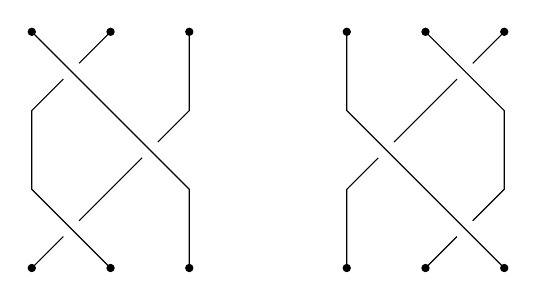
\begin{tikzpicture}
        \begin{scope}
            \draw[black,fill=black] (0, 0) circle (.3ex);
            \draw[black,fill=black] (1, 0) circle (.3ex);
            \draw[black,fill=black] (2, 0) circle (.3ex);
            \draw[black,fill=black] (0, 3) circle (.3ex);
            \draw[black,fill=black] (1, 3) circle (.3ex);
            \draw[black,fill=black] (2, 3) circle (.3ex);
            \draw (0, 3) -- (1, 2) -- (2, 1) -- (2, 0);
            \draw (1, 3) -- (0.6, 2.6);
            \draw (0.4, 2.4) -- (0, 2) -- (0, 1) -- (1, 0);
            \draw (2, 3) -- (2, 2) -- (1.6, 1.6);
            \draw (1.4, 1.4) -- (0.6, 0.6);
            \draw (0.4, 0.4) -- (0, 0);
        \end{scope}
        \node at (3cm,1.5cm) {$\isom$};
        \begin{scope}[xshift=4cm]
            \draw[black,fill=black] (0, 0) circle (.3ex);
            \draw[black,fill=black] (1, 0) circle (.3ex);
            \draw[black,fill=black] (2, 0) circle (.3ex);
            \draw[black,fill=black] (0, 3) circle (.3ex);
            \draw[black,fill=black] (1, 3) circle (.3ex);
            \draw[black,fill=black] (2, 3) circle (.3ex);
            \draw (0, 3) -- (0, 2) -- (1, 1) -- (2, 0);
            \draw (1, 3) -- (2, 2) -- (2, 1) -- (1.6, 0.6);
            \draw (1.4, 0.4) -- (1, 0);
            \draw (2, 3) -- (1.6, 2.6);
            \draw (1.4, 2.4) -- (0.6, 1.6);
            \draw (0.4, 1.4) -- (0, 1) -- (0, 0);
        \end{scope}
    \end{tikzpicture} \]
    This relation precisely corresponds to the quantum Yang--Baxter equation.
\end{example}

\begin{topic}{chevalley-shephard-todd-theorem}{Chevalley--Shephard--Todd theorem}
    Let $V$ be a finite-dimensional \tref{LA:vector-space}{vector space} over a \tref{field}{field} $k$, and $G \subset \textup{GL}(V)$ a finite \tref{GT:group}{group} whose \tref{GT:order}{order} $|G|$ is invertible in $k$. An element $s \in \textup{GL}(V)$ is a \textit{pseudoreflection} if $s \ne 1$ and $s$ fixes a codimension $1$ subspace of $V$. The \textbf{Chevalley--Shephard--Todd theorem} states that the following are equivalent:
    \begin{enumerate}[label=(\roman*)]
        \item $G$ is generated by pseudoreflections,
        \item the ring of invariants $k[V]^G$ is a free polynomial algebra over $k$,
        \item $k[V]$ is a \tref{free-module}{free module} over $k[V]^G$.
    \end{enumerate}
\end{topic}

\begin{example}{chevalley-shephard-todd-theorem}
    Let $G = \ZZ/2\ZZ$ act on $V = k^2$ by $(x, y) \mapsto (x, -y)$. Then $G$ is generated by a pseudoreflection, and indeed
    \[ k[x, y]^G = k[x, y^2] \]
    a free polynomial algebra over $k$. However, if we let $G$ act on $V$ by $(x, y) \mapsto (-x, -y)$, then $G$ is not generated by pseudoreflections, and indeed
    \[ k[x, y]^G = k[x^2, xy, y^2] = k[u, v, w] / (w^2 - uv) \]
    is not a free polynomial algebra over $k$.
\end{example}

\begin{example}{chevalley-shephard-todd-theorem}
    Consider the \tref{GT:symmetric-group}{symmetric group} $S_n$ acting on $V = k^{n - 1}$ via the \tref{RT:standard-representation}{standard representation}. Note that any $2$-cycle acts by a pseudo-reflection, and since $S_n$ is generated by $2$-cycles, we can conclude that $k[V]^G$ is a free polynomial algebra over $k$.
\end{example}

\begin{topic}{molien-formula}{Molien's formula}
    Let $G$ be a finite \tref{GT:group}{group} and $\rho : G \to \textup{GL}(V)$ a finite-dimensional complex \tref{RT:representation}{representation}. Then $G$ acts naturally on the \tref{symmetric-algebra}{symmetric algebra} $\textup{Sym}(V)$. \textbf{Molien's formula} states that the \tref{hilbert-series}{Hilbert series} of the invariant subalgebra $\textup{Sym}(V)^G \subset \textup{Sym}(V)$ is given by
    \[ \textup{HS}_{\textup{Sym}(V)^G}(t) = \frac{1}{|G|} \sum_{g \in G} \frac{1}{\det(1 - gt)} . \]
\end{topic}

\begin{example}{molien-formula}
    \begin{proof}
        Write $S = \textup{Sym}(V)$. The \textit{Reynolds operator} $R^G : S \to S$ given by $f \mapsto \frac{1}{|G|} \sum_{g \in G} g \cdot f$ projects $S_d$ onto $S^G_d$ for each $d \ge 0$, so
        \[ \dim_\CC(S_d) = \tr_{S_d}(R^G) = \frac{1}{|G|} \sum_{g \in G} \tr_{S_d}(g) . \]
        % Hence, it suffices to show that 
        % \[ \sum_{d \ge 0} \tr_{S_d}(g) \cdot t^d = \frac{1}{\det(1 - gt)} \]
        % for all $g \in G$.
        Now fix $g \in G$, and let $\lambda_1, \ldots, \lambda_n$ be the eigenvalues of $\rho(g)$. Then the eigenvalues of $g$ acting on $S_d$ are given by $\mu_\alpha = \prod_{i = 1}^{n} \lambda_i^{\alpha_i}$ for each $\alpha \in \NN^n$ with $\alpha_1 + \ldots + \alpha_n = d$. Now it follows that
        \[ \sum_{d \ge 0} \tr_{S_d}(g) \cdot t^d = \sum_{\alpha} \prod_{i = 1}^{n} (\lambda_i t)^{\alpha_i} = \prod_{i = 1}^{n} \sum_{j \ge 0} (\lambda_i t)^j = \prod_{i = 1}^{n} \frac{1}{1 - \lambda_i t} = \frac{1}{\det(1 - gt)} . \]
        Combined with the above equation, the result follows.
    \end{proof}
\end{example}

\begin{topic}{ring}{ring}
    A \textbf{ring} is an abelian group $R$ with an operation called multiplication and an element $1 \in R$ satisfying
    \begin{itemize}
        \item (\textit{associativity}) $a(bc) = (ab)c$,
        \item (\textit{distributivity}) $a(b + c) = ab + ac$ and $(a + b)c = ac + bc$,
        \item (\textit{unit}) $1 \cdot a = a \cdot 1 = a$,
    \end{itemize}
    for all $a, b, c \in R$.
    
    A ring $R$ is called \textbf{commutative} if moreover $ab = ba$ for all $a, b \in R$.
\end{topic}

\begin{topic}{ring-morphism}{ring morphism}
    A map $f : R \to S$ between \tref{ring}{rings} is a \textbf{ring morphism} if
    \begin{itemize}
        \item $f(1) = 1$,
        \item $f(a + b) = f(a) + f(b)$,
        \item $f(ab) = f(a) f(b)$,
    \end{itemize}
    for all $a, b \in R$.
\end{topic}

\begin{topic}{unit}{unit}
    Let $R$ be a \tref{ring}{ring}. An element $a \in R$ is called a \textbf{unit} if there exists some $b \in R$ such that $ab = 1$. This is denoted $b = a^{-1}$.
\end{topic}

\begin{topic}{irreducible-element}{irreducible element}
    Let $R$ be a \tref{domain}{domain}. An element $a \in R$ is called a \textbf{irreducible} if $a$ is not a \tref{unit}{unit}, and for all $b, c \in R$ such that $bc = a$ either $b$ or $c$ is a unit.
\end{topic}

\begin{topic}{zero-divisor}{zero-divisor}
    Let $R$ be a \tref{ring}{ring}. An element $a \in R$ is called a \textbf{zero-divisor} if $a \ne 0$ and $ab = 0$ for some $b \ne 0$.
\end{topic}

\begin{topic}{nilpotent-element}{nilpotent element}
    Let $R$ be a \tref{ring}{ring}. An element $a \in R$ is \textbf{nilpotent} if $a^n = 0$ for some positive integer $n$.
\end{topic}

\begin{topic}{domain}{domain}
    A non-zero commutative \tref{ring}{ring} $R$ is called a \textbf{domain} if it has no zero-divisors, that is, $ab = 0$ implies $a = 0$ or $b = 0$ for all $a, b \in R$.
\end{topic}

\begin{topic}{field}{field}
    A commutative \tref{ring}{ring} $R$ is called a \textbf{field} if all non-zero elements are units, that is, for all non-zero $a \in R$ there exists a $b \in R$ such that $ab = 1$. 
\end{topic}

\begin{topic}{ideal}{ideal}
    Let $R$ be a \tref{ring}{ring}. An \textbf{ideal} of $R$ is a subset $I \subset R$ such that
    \begin{itemize}
        \item $I$ is a subgroup of $R$ under addition,
        \item (\textit{left-ideal}) $ra \in I$  for all $r \in R$ and $a \in I$,
        \item (\textit{right-ideal}) $ar \in I$ for all $r \in R$ and $a \in I$.
    \end{itemize}
\end{topic}

\begin{topic}{coprime-ideals}{coprime ideals}
    Two \tref{ideal}{ideals} $I, J$ of a commutative \tref{ring}{ring} $R$ are \textbf{coprime} if $I + J = R$.
\end{topic}

\begin{topic}{radical-ideal}{radical ideal}
    Let $R$ be a \tref{ring}{ring}. The \textbf{radical} of an ideal $I \subset R$ is given by
    \[ \sqrt{I} = \{ x \in R : x^n \in I \} . \]
    An ideal $I$ is called \textbf{radical} if $I = \sqrt{I}$.
\end{topic}

\begin{topic}{principal-ideal}{principal ideal}
    A \textbf{principal ideal} is an \tref{ideal}{ideal} $I \subset R$ generated by a single element, that is, of the form
    \[ I = (a) = \{ r a : r \in R \} \]
    for some $a \in R$.
\end{topic}

\begin{topic}{prime-ideal}{prime ideal}
    Let $R$ be a \tref{ring}{ring}. An \tref{ideal}{ideal} $I \subset R$ is called \textbf{prime} if $I \ne R$ and
    \[ ab \in I \implies a \in I \text{ or } b \in I . \]
    
    Equivalently, $I \subset R$ is a prime ideal iff the quotient ring $R / I$ is a \tref{domain}{domain}.
\end{topic}

\begin{topic}{maximal-ideal}{maximal ideal}
    Let $R$ be a \tref{ring}{ring}. An \tref{ideal}{ideal} $I \subset R$ is called \textbf{maximal} if $I \ne R$ and
    \[ I \subset J \subsetneq R \text{ for some ideal } J \subset R \implies I = J . \]
    
    Equivalently, $I \subset R$ is a maximal ideal iff the quotient ring $R / I$ is a \tref{field}{field}.
    
    Every maximal ideal is \tref{prime-ideal}{prime}.
\end{topic}

\begin{topic}{irreducible-ideal}{irreducible ideal}
    Let $R$ be a \tref{ring}{ring}. An \tref{ideal}{ideal} $I \subset R$ is called \textbf{irreducible} if
    \[ I = J_1 \cap J_2 \quad \implies \quad I = J_1 \text{ or } I = J_2 . \]
\end{topic}

\begin{topic}{local-ring}{local ring}
    A \textbf{local ring} is a \tref{ring}{ring} $R$ with exactly one \tref{maximal-ideal}{maximal ideal}. The maximal is often denoted by $\mathfrak{m}$.
    
    The quotient $k = R/\mathfrak{m}$ is called the \textbf{residue field}.
\end{topic}

\begin{topic}{local-morphism}{local morphism}
    A \textbf{local morphism} of \tref{local-ring}{local rings} $f : R \to S$ is a ring morphism such that $f(\mathfrak{m}_R) \subset \mathfrak{m}_S$.
\end{topic}

\begin{topic}{finite-type}{finite type}
    A ring morphism $R \to S$ is said to be of \textbf{finite type} if $S$ is isomorphic to a quotient of $R[x_1, \ldots, x_n]$ for some integer $n$.
    
    In this case, $S$ is also said to be a \textbf{finitely generated $R$-algebra}.
\end{topic}

\begin{topic}{finite-presentation}{finite presentation}
    A ring morphism $R \to S$ is said to be of \textbf{finite presentation} if $S$ is isomorphic to $R[x_1, \ldots, x_n] / (f_1, \ldots, f_m)$ for some integer $n$ and some $f_i \in R[x_1, \ldots, x_n]$.
    
    In this case, $S$ is also said to be a \textbf{finitely presented $R$-algebra}.
\end{topic}

\begin{topic}{krull-dimension}{Krull dimension}
    The \textbf{Krull dimension} of a commutative ring $R$ is the supremum of the lengths of all chains of \tref{prime-ideal}{prime ideals}, where a chain of the form
    \[ \mathfrak{p}_0 \subsetneq \mathfrak{p}_1 \subsetneq \cdots \subsetneq \mathfrak{p}_n \]
    has length $n$.
\end{topic}

\begin{topic}{group-ring}{group ring}
    Let $R$ be a \tref{ring}{ring} and $G$ a group. The \textbf{group ring} $R[G]$ of $G$ over $R$ is defined as
    \[ R[G] = \bigoplus_{g \in G} R , \]
    where multiplication is induced by
    \[ (a \cdot g) \cdot (b \cdot h) = (ab) \cdot gh . \]
    % where multiplication is given by
    % \[ (a_g)_{g \in G} \cdot (b_g)_{g \in G} = \left(\sum_{h \in G} a_h b_{h^{-1}g}\right)_{g \in G} \]
\end{topic}

\begin{topic}{chinese-remainder-theorem}{Chinese remainder theorem}
    Let $R$ be a commutative \tref{ring}{ring} and suppose $I, J$ are coprime ideals of $R$, i.e. $I + J = R$. Then the \textbf{Chinese remainder theorem} states that $I \cap J = I \cdot J$ and that there is an isomorphism of rings
    \[ R / (I \cdot J) \xrightarrow{\sim} (R / I) \times (R/J), \qquad a \text{ mod } (I \cdot J) \mapsto (a \text{ mod } I, b \text{ mod } J) . \]
    
    In particular, when $R = \ZZ$ with $I = (n)$ and $J = (m)$ for $n, m$ relatively prime, there is
    \[ \ZZ / nm \ZZ \simeq (\ZZ/n\ZZ) \times (\ZZ/m\ZZ), \qquad a \text{ mod } nm \mapsto (a \text{ mod } n, a \text{ mod } m) . \]
\end{topic}

\begin{topic}{idempotent}{idempotent}
    An element $e \in R$ of a \tref{ring}{ring} $R$ is called \textbf{idempotent} if $e^2 = e$.
\end{topic}

\begin{topic}{dual-numbers}{dual numbers}
    Let $R$ be a commutative \tref{ring}{ring}. The \textbf{ring of dual numbers} over $R$ is the quotient ring
    \[ R[\varepsilon] / (\varepsilon^2) . \]
\end{topic}

\begin{topic}{noetherian-ring}{noetherian ring}
    A commutative \tref{ring}{ring} $R$ is called \textbf{noetherian} if it satisfies the \textit{ascending chain condition}: for any increasing sequence of ideals
    \[ I_1 \subset I_2 \subset I_3 \subset \cdots \]
    there exists some $N \in \NN$ such that $I_n = I_N$ for any $n \ge N$.
    
    Equivalently, $R$ is noetherian if all its ideals are finitely generated.
\end{topic}

\begin{example}{noetherian-ring}
    The following are all noetherian rings.
    \begin{itemize}
        \item Any \tref{field}{field}: their only ideal is $(0)$.
        \item Any \tref{principal-ideal-domain}{PID}: every ideal is generated by a single element.
        \item If $R$ is noetherian, then so is $R[x]$: this is \textit{Hilbert's basis theorem}.
    \end{itemize}
\end{example}

\begin{example}{noetherian-ring}
    The ring $k[x_1, x_2, x_3, \ldots]$ is not noetherian. Namely, the sequence of ideals
    \[ (x_1) \subset (x_1, x_2) \subset (x_1, x_2, x_3) \subset \ldots \]
    is ascending, but does not stabilize.
\end{example}

\begin{topic}{localization}{localization}
    Let $R$ be a commutative \tref{ring}{ring}, and $S \subset R$ a \textit{multiplicative set} (that is, $1 \in S$ and $xy \in S$ for all $x, y \in S$). Then the \textbf{localization} of $R$ w.r.t. $S$ is the ring
    \[ S^{-1} R = R \times S / \sim{} \quad \text{ where } (r_1, s_1) \sim{} (r_2, s_2) \text{ if } t(r_1 s_2 - r_2 s_1) = 0 \text{ for some } t \in S . \]
\end{topic}

\begin{example}{localization}
    If $R$ is a \tref{domain}{domain}, then $S = R - \{ 0 \}$ is a multiplicative set, and $S^{-1} R$ is the \tref{field-of-fractions}{field of fractions} of $R$.
\end{example}

\begin{example}{localization}
    For any commutative ring $R$ and $f \in R$, the set
    \[ S = \{ 1, f, f^2, \ldots \} \]
    is a multiplicative set, and the localization is
    \[ R_f := S^{-1} R = \left\{ \frac{a}{f^n} : a \in R, \; n \ge 0 \right\} . \]
\end{example}

\begin{example}{localization}
    For any commutative ring $R$ and \tref{prime-ideal}{prime ideal} $\mathfrak{p}$, the set
    \[ S = \{ f \in R : f \not\in \mathfrak{p} \} \]
    is a multiplicative set, and the localization
    \[ R_\mathfrak{p} := S^{-1} R = \left\{ \frac{f}{g} : f, g \in R, \; g \not\in \mathfrak{p} \right\} \]
    is a \tref{local-ring}{local ring} with maximal ideal $\mathfrak{p} R_\mathfrak{p}$.
\end{example}

\begin{topic}{regular-ring}{regular (local) ring}
    A \textbf{regular local ring} is a commutative \tref{noetherian-ring}{noetherian} \tref{local-ring}{local} ring such that the minimal number of generators of its maximal ideal is equal to its \tref{krull-dimension}{Krull dimension}. Equivalently, a local ring $R$ with maximal ideal $\mathfrak{m}$ and residue field $k = R / \mathfrak{m}$ is regular iff $\dim_k(\mathfrak{m} / \mathfrak{m}^2) = \dim R$.
    
    A \textbf{regular ring} is a commutative noetherian ring, such that the \tref{localization}{localization} at every \tref{prime-ideal}{prime ideal} is a regular local ring.
\end{topic}

\begin{example}{regular-ring}
    Every field is a regular local ring: their Krull dimension is zero, and their maximal ideal is $(0)$.
\end{example}

\begin{example}{regular-ring}
    The local ring $R = k[x]/(x^2)$ is not a regular local ring. Its only prime ideal is its maximal ideal $\mathfrak{m} = (x)/(x^2)$, so the Krull dimension is zero, but the minimal number of generators of $\mathfrak{m}$ is one.
\end{example}

\begin{topic}{principal-ideal-domain}{principal ideal domain (PID)}
    A \textbf{principal ideal domain} (PID) is a \tref{domain}{domain} $R$ in which every \tref{ideal}{ideal} is \tref{principal-ideal}{principal}. That is, every ideal $I \subset R$ is of the form $I = (x)$ for some element $x \in R$.
\end{topic}

\begin{topic}{unique-factorization-domain}{unique factorization domain (UFD)}
    A \textbf{unique factorization domain} (UFD) is a \tref{domain}{domain} $R$ for which every non-zero $x \in R$ can be written as the product of a \tref{unit}{unit} and a finite number of \tref{irreducible-element}{irreducible} elements:
    \[ a = u \cdot p_1 \cdot p_2 \cdot \cdots \cdot p_k \qquad u \in R^\times, \; k \ge 0, \; p_i \in R \text{ irreducible}. \]
\end{topic}

\begin{topic}{euclidean-ring}{Euclidean ring}
    A \textbf{Euclidean ring} is a \tref{domain}{domain} $R$ for which there exists a function
    \[ g : R^\times \to \ZZ_{\ge 0} \]
    such that for all $a, b \in R$ with $b \ne 0$, there exists $q, r \in R$ with $a = qb + r$ and either $r = 0$ or $g(r) < g(b)$.
    
    That is, a ring in which one can perform division with remainder. The function $g$ is used to say that the `remainder' $r$ is `smaller' than the element $b$ one divides by.
    
    In particular, one can find the \textit{gcd} of elements by means of the \textit{Euclidean algorithm}.
\end{topic}

\begin{topic}{field-of-fractions}{field of fractions}
    The \textbf{field of fractions} of a \tref{domain}{domain} $R$ is the \tref{field}{field} given by
    \[ K = \left\{ (a, b) : a, b \in R, b \ne 0 \right\} / \sim{} \]
    where $(a, b) \sim{} (c, d)$ iff $ad = bc$. Indeed $(a, b)$ represents the fraction $\frac{a}{b}$. Addition and multiplication are given by
    \[ \frac{a}{b} + \frac{c}{d} = \frac{ad + bc}{bd} \quad \text{and} \quad \frac{a}{b} \cdot \frac{c}{d} = \frac{ac}{bd} . \]
\end{topic}

\begin{example}{field-of-fractions}
    The field of fractions of $\ZZ$ is $\QQ$.
\end{example}

\begin{topic}{valuation-ring}{valuation ring}
    A \textbf{valuation ring} is a \tref{domain}{domain} $R$ such that for every element $x$ of its \tref{field-of-fractions}{field of fractions}, at least one of $x$ or $x^{-1}$ belongs to $R$.
\end{topic}

\begin{topic}{discrete-valuation-ring}{discrete valuation ring}
    A domain \tref{domain}{domain} $R$ is a \textbf{discrete valuation ring} if there is a \textit{discrete valuation} $v$ of its \tref{field-of-fractions}{field of fractions} $K$, such that $R$ is the \textit{valuation ring} of $v$. This means there is a homomorphism
    \[ v : K^\times \to \ZZ \]
    such that
    \[ R = \{ x \in K : v(x) \ge 0 \} . \]
    
    In particular, $R$ is \tref{local-ring}{local} with maximal ideal $\mathfrak{m} = \{ x \in K : v(x) > 0 \}$. Indeed, any element $x \in R$ with $v(x) = 0$ is a unit in $R$.
\end{topic}

\begin{example}{discrete-valuation-ring}
    Let $K = \QQ$ and fix a prime number $p$. Any non-zero $x \in \QQ$ can be written uniquely as $x = p^m y$ where $k \in \ZZ$ and both the numerator and denominator of $y$ are coprime to $p$. Now define the discrete valuation $v_p(x) = m$, then the valuation ring is the local ring $\ZZ_{(p)}$.
\end{example}

% \begin{topic}{dedekind-domain}{Dedekind domain}
%     A \textbf{Dedekind domain} is a \tref{domain}{domain} in which every non-zero proper ideal factors into a product of prime ideals.
% \end{topic}

\begin{topic}{monic-polynomial}{monic polynomial}
    A polynomial $f$ is called \textbf{monic} if its leading coefficient is $1$.
\end{topic}

\begin{topic}{integral-element}{integral element}
    Let $A$ be a commutative \tref{ring}{ring}, and $B$ an $A$-algebra. An element $x \in B$ is said to be \textbf{integral} over $A$ if $x$ is a root of a monic polynomial with coefficients in $A$. That is,
    \[ x^n + a_1 x^{n - 1} + \cdots + a_n = 0 \]
    for some $a_i \in A$.
\end{topic}

\begin{topic}{integral-closure}{integral closure}
    Let $A$ be a commutative \tref{ring}{ring}, and $B$ an $A$-algebra. The \textbf{integral closure} of $A$ in $B$ is the subring of $B$ of elements which are \tref{integral-element}{integral} over $A$.
    
    If the integral closure is equal to $A$, then $A$ is said to be \textbf{integrally closed} in $B$. If the integral closure is equal to $B$, the ring $B$ is said to be \textbf{integral} over $A$.
\end{topic}

\begin{topic}{artin-ring}{artin ring}
    A commutative \tref{ring}{ring} $R$ is called \textbf{artin} if it satisfies the \textit{descending chain condition}: for any decreasing sequence of ideals
    \[ I_1 \supset I_2 \supset I_3 \supset \cdots \]
    there exists some $N \in \NN$ such that $I_n = I_N$ for any $n \ge N$.
\end{topic}

\begin{topic}{fractional-ideal}{fractional ideal}
    Let $R$ be a \tref{domain}{domain} and $K$ its \tref{field-of-fractions}{field of fractions}. An $R$-submodule $M$ of $K$ is a \textbf{fractional ideal} of $R$ if $xM \subset R$ for some $x \ne 0$ in $R$.
\end{topic}

\begin{topic}{invertible-ideal}{invertible ideal}
    Let $R$ be a \tref{domain}{domain} and $K$ its \tref{field-of-fractions}{field of fractions}. An $R$-submodule $M$ of $K$ is an \textbf{invertible ideal} if there exists a submodule $N$ of $K$ such that $MN = R$. This module $N$ is then unique and equal to
    \[ N = (R : M) := \{ x \in K : xM \subset R \} . \]
    
    The invertible ideals form a group with respect to multiplication, whose unit element is $R = (1)$.
\end{topic}

\begin{topic}{syzygy-module}{syzygy module}
    Let $g_1, g_2, \ldots, g_k$ be generators of \tref{module}{module} $M$ over a commutative \tref{ring}{ring} $R$. The \textbf{syzygy module} is the $R$-module consisting of all relations between the generators, i.e. the kernel of
    \[ \bigoplus_{i = 1}^{k} R \to M, \qquad (r_1, \ldots, r_k) \mapsto r_1 g_1 + \cdots r_k g_k . \]
    Inductively, one can define the $n$-th syzygy module for any $n \ge 1$ after choosing generators.
\end{topic}

% Hilbert's three theorems
\begin{topic}{hilbert-basis-theorem}{Hilbert's basis theorem}
    \textbf{Hilbert's basis theorem} states that if a commutative \tref{ring}{ring} $R$ is \tref{noetherian-ring}{noetherian}, then so is the polynomial ring $R[x]$.
\end{topic}

% \begin{topic}{hilbert-nullstellensatz}{Hilbert's Nullstellensatz}
%     \textbf{Hilbert's Nullstellensatz} states that there is a bijection
%     \[ \left\{ \begin{array}{c} \text{radical ideals of} \\ k[x_1, \ldots, x_n] \end{array} \right\} \leftrightarrow \left\{ \begin{array}{c} \text{closed subsets} \\ \text{of $\AA^n$} \end{array} \right\} \]
%     \[ I \mapsto Z(I) \]
%     \[ I \mapsfrom Z(I) \]
% \end{topic}

\begin{topic}{hilbert-syzygy-theorem}{Hilbert's syzygy theorem}
    \textbf{Hilbert's syzygy theorem} states that if $M$ is a finitely generated module over a polynomial ring $k[x_1, \ldots, x_n]$, then the $n$-th \tref{syzygy-module}{syzygy module} $M$ is always \tref{free-module}{free}.
    
    In particular, this implies that there exists a free resolution
    \[ 0 \to F_k \to F_{k - 1} \to \cdots \to F_0 \to M \to 0 \]
    of length $k \le n$.
\end{topic}

\begin{topic}{primary-ideal}{primary ideal}
    Let $R$ be a commutative \tref{ring}{ring}. An \tref{ideal}{ideal} $\mathfrak{q}$ of $R$ is \textbf{primary} if $\mathfrak{q} \ne R$ and if
    \[ xy \in \mathfrak{q} \implies \text{ either } x \in \mathfrak{q} \text{ or } y^n \in \mathfrak{q} \text{ for some } n > 0 . \]
    In other words,
    \[ \mathfrak{q} \text{ is primary } \iff A / \mathfrak{q} \ne 0 \text{ and every zero-divisor in } A / \mathfrak{q} \text{ is nilpotent} . \]
\end{topic}

\begin{topic}{primary-decomposition}{primary decomposition}
    Let $R$ be a commutative \tref{ring}{ring}. A \textbf{primary decomposition} of an ideal $I \subset R$ is an expression of $I$ as a finite intersection of \tref{primary-ideal}{primary ideals},
    \[ I = \bigcap_{i = 1}^{n} \mathfrak{q}_i . \]
    
    The primary decomposition is said to be \textbf{minimal} if (i) the $\mathfrak{p}_i = r(\mathfrak{q}_i)$ are all distinct, and (ii) no $\mathfrak{q}_i$ contains the intersection of the other primary ideals.
\end{topic}

\begin{topic}{annihilator}{annihilator}
    Let $R$ be a commutative \tref{ring}{ring} and $M$ an $R$-module. The \textbf{annihilator} of $M$ is the subring
    \[ \text{Ann}(M) = \{ x \in R : xM = 0 \} \]
\end{topic}

\begin{topic}{nilradical}{nilradical}
     The \textbf{nilradical} of a commutative \tref{ring}{ring} $R$ is the ideal of \tref{nilpotent-element}{nilpotent} elements
     \[ \mathfrak{N}_R = \{ x \in R : x \text{ is nilpotent } \} . \]
     It is equal to the intersection of all prime ideals of $R$,
     \[ \mathfrak{N}_R = \bigcap_{\mathfrak{p} \subset R \text{ prime}} \mathfrak{p} . \]
\end{topic}

\begin{topic}{jacobson-radical}{Jacobson radical}
     The \textbf{Jacobson radical} of a commutative \tref{ring}{ring} $R$ is the ideal given by the intersection of all \tref{maximal-ideal}{maximal} ideals,
     \[ \mathfrak{J}_R = \bigcap_{\mathfrak{m} \subset R \text{ maximal}} \mathfrak{m} . \]
     It can also be characterized by
     \[ x \in \mathfrak{J}_R \iff 1 - xy \text{ is a unit for all } y \in R . \]
\end{topic}

\begin{topic}{regular-sequence}{regular sequence}
    Let $R$ be a commutative \tref{ring}{ring}, and $M$ an $R$-module. An $M$-\textbf{regular sequence} is a sequence
    \[ r_1, r_2, \ldots, r_d \in R \]
    such that $r_i$ is not a \textit{zero-divisor} on $M/(r_1, \ldots, r_{i - 1})$. That is, if $r_i m = 0$ for some $m \in M / (r_1, \ldots, r_{i - 1})$, then $m = 0$.
    
    When $M = R$, such a sequence is simply called a \textbf{regular sequence}.
\end{topic}

\begin{example}{regular-sequence}
    Consider $R = k[x, y]$ and the sequence $(xy, x^2)$. This sequence is not regular, since $x^2 \cdot y = 0$ in $\QQ[x, y] / (xy)$, although $y \ne 0$.
\end{example}

\begin{example}{regular-sequence}
    Consider $R = k[x, y, z]$ and the sequence $(x, y(1 - x), z(1 - x))$. This sequence is regular since
    \[ y(1 - x) = y \in k[x, y, z]/(x) = k[y, z] \quad \text{ and } \quad z(1 - x) = z \in k[x, y, z]/(x, y - xy) = k[z] \]
    are both non-zero-divisors.
    
    However, note that the order matters as $(y(1 - x), z(1 - x), x)$ is not a regular sequence. Namely, $z(1 - x) \cdot y = 0 \in k[x, y, z] / (y(1 - x))$ even though $y \ne 0$.
\end{example}

\begin{topic}{hilbert-series}{Hilbert series}
    Let $S = \bigoplus_{i \ge 0} S_i$ be a finitely generated graded commutative algebra over a field $k$, with $S_0 = k$. The \textbf{Hilbert series} of $S$ is defined as
    \[ \text{H}_S(t) = \sum_{i = 0}^{\infty} \dim_k S_i \cdot t^i . \]
\end{topic}

\begin{example}{hilbert-series}
    Let $R = k[x_1, \ldots, x_n]$ and $I = (f)$ for some homogenous polynomial of degree $d$. Then we have an exact sequence (a free resolution)
    \[ 0 \to R(-d) \xrightarrow{\cdot f} R \to R / I \to 0 , \]
    which implies that
    \[ \text{H}_{R/I}(t) = \text{H}_R(t) - \text{H}_{R(-d)}(t) = \text{H}_R(t) (1 - t^d) = \frac{1 - t^d}{(1 - t)^n}. \]
\end{example}

\begin{topic}{absolutely-flat-ring}{absolutely flat ring}
    A commutative \tref{ring}{ring} $R$ is called \textbf{absolutely flat} if every $R$-module is \tref{flat-module}{flat}.
\end{topic}

\begin{topic}{standard-smooth}{standard smooth}
    Let $A$ be commutative \tref{ring}{ring}, and $B = A[x_1, \ldots, x_n] / (f_1, \ldots, f_c)$ a finitely presented $A$-algebra. Then $B$ is a \textbf{standard smooth} over $A$ if the determinant
    \[ \det \begin{pmatrix}
        \frac{\partial f_1}{\partial x_1} & \frac{\partial f_1}{\partial x_2} & \cdots & \frac{\partial f_1}{\partial x_c} \\
        \frac{\partial f_2}{\partial x_1} & \frac{\partial f_2}{\partial x_2} & \cdots & \frac{\partial f_2}{\partial x_c} \\ 
        \vdots & \vdots & \ddots & \vdots \\ 
        \frac{\partial f_c}{\partial x_1} & \frac{\partial f_c}{\partial x_2} & \cdots & \frac{\partial f_c}{\partial x_c}
    \end{pmatrix} \]
    maps to an invertible element in $B$. Note that this definition is dependent on the presentation of $B$!
\end{topic}

\begin{example}{standard-smooth}
    Take $A = k$ a field and $B = k[x, y] / (xy)$. Then $\partial (xy) / \partial x = y$ which is not invertible in $B$, so $k[x, y] / (xy)$ is not standard smooth over $k$.
    
    Taking $C = k[x, y] / (xy - 1)$, we see that $\partial (xy - 1) / \partial x = y$, which is invertible in $C$. Hence $k[x, y] / (xy - 1)$ is standard smooth over $k$.
\end{example}

\begin{topic}{etale-algebra}{étale algebra}
    Let $A$ be a commutative \tref{ring}{ring} and $B$ an $A$-algebra. Then $B$ is an \textbf{étale algebra} over $A$ if $B$ is a \tref{flat-module}{flat} $A$-module and $\Omega_{B/A} = 0$.
\end{topic}

\begin{topic}{fitting-ideal}{Fitting ideal}
    Let $R$ be a commutative \tref{ring}{ring} and $M$ an $R$-\tref{module}{module} generated by elements $m_1, \ldots, m_n \in M$, with relations
    \[ a_{i1} m_1 + \cdots a_{in} m_n = 0 \text{ for } i = 1, 2, \ldots, \ell . \]
    Then the \textbf{$i$-th Fitting ideal} $\text{Fitt}_i(M)$ of $M$ is generated by the minors (determinants of submatrices) of order $n - i$ of the matrix $a_{ij}$. It can be shown that this does not depend on the choice of generators or relations. One has the inclusions
    \[ \text{Fitt}_0(M) \subset \text{Fitt}_1(M) \subset \text{Fitt}_2(M) \subset \cdots \]
    Intuitively, the $i$-th fitting ideal (or actually the quotient $R / \text{Fitt}_i(M)$) measures the obstruction for $M$ to be generated by $i$ elements.
    
    Sometimes the \textbf{Fitting ideal} of $M$ is defined as the first non-zero fitting ideal.
\end{topic}

\begin{example}{fitting-ideal}
    If $M$ is \tref{free-module}{free} of rank $n$, the matrix $a_{ij}$ will be of size $0 \times n$. Hence $\text{Fitt}_i(M) = 0$ for $i < n$ as there are no submatrices of size $n - i > 0$, and $\text{Fitt}_i(M) = R$ for $i \ge n$ as the determinant of a $0 \times 0$ matrix is one.
\end{example}

\begin{example}{fitting-ideal}
    Consider $M = \ZZ / p \ZZ \times \ZZ / p^2 \ZZ$ as $\ZZ$-module. It can be generated by $m_1 = (1, 0)$ and $m_2 = (0, 1)$ with relations $p m_1 = 0$ and $p^2 m_2 = 0$, so the corresponding matrix is
    \[ a_{ij} = \begin{pmatrix} p & 0 \\ 0 & p^2 \end{pmatrix} \]
    and thus
    \[ \text{Fitt}_0(M) = (p^3), \quad \text{Fitt}_1(M) = (p, p^2) = (p) \quad \text{ and } \quad \text{Fitt}_{\ge 2}(M) = \ZZ . \]
\end{example}

\begin{example}{fitting-ideal}
    Consider the finitely generated abelian group $M = \ZZ^r \times \ZZ / d_1 \ZZ \times \cdots \times \ZZ / d_k \ZZ$ with $d_1 | d_2 | \cdots | d_k$. Using the natural generators, the relation matrix is
    \[ a_{ij} = \begin{pmatrix} \textbf{0}_{r \times r} & & &  \\  & d_1 & \\ & & \ddots & \\ & & & d_k \end{pmatrix} \]
    and thus
    \[ \begin{array}{rcl}
         \text{Fitt}_{0 \le i \le r}(M) &=& (0) , \\
        \text{Fitt}_{r + 1}(M) &=& (d_1 d_2\cdots d_k) , \\
        \text{Fitt}_{r + 2}(M) &=& (d_1 d_2\cdots d_{k - 1}) , \\
        & \vdots & \\
        \text{Fitt}_{r + k - 1}(M) &=& (d_1) , \\
        \text{Fitt}_{\ge r + k}(M) &=& \ZZ .
    \end{array} \]
\end{example}

\begin{example}{fitting-ideal}
    Consider the scheme $X = \Spec k[x_1, \ldots, x_n] / I$ with $I = (f_1, \ldots, f_k)$ for some polynomials $f_i$. The module of differentials
    \[ \Omega_{X/k} = \left(\bigoplus_{i = 1}^{n} k[x_1, \ldots, x_n] / I \cdot dx_i \right) / (df_1, df_2, \ldots, df_k) \]
    is generated by $dx_1, \ldots, dx_n$ and relations
    \[ df_i = \sum_{j = 1}^{n} \frac{\partial f_i}{\partial x_j} dx_j = 0 \quad \text{ for } i = 1, 2, \ldots, k , \]
    so the corresponding matrix is the Jacobian matrix
    \[ J = \begin{pmatrix}
        \frac{\partial f_1}{\partial x_1} & \frac{\partial f_1}{\partial x_2} & \cdots & \frac{\partial f_1}{\partial x_n} \\
        \frac{\partial f_2}{\partial x_1} & \frac{\partial f_2}{\partial x_2} & \cdots & \frac{\partial f_2}{\partial x_n} \\
        \vdots & \vdots & \ddots & \vdots \\
        \frac{\partial f_k}{\partial x_1} & \frac{\partial f_k}{\partial x_2} & \cdots & \frac{\partial f_k}{\partial x_n}
    \end{pmatrix} . \]
    Now $X$ is smooth over $k$ if and only if $\Omega_{X/k}$ is locally free of rank $n = \dim X$, which is equivalent to the Fitting ideal $\text{Fitt}_{\dim X}(\Omega_{X/k})$ generating the unit ideal in the localization of each prime ideal of $k[x_1, \ldots, x_n] / I$, which is equivalent to the Fitting ideal $\text{Fitt}_{\dim X}(\Omega_{X/k})$ generating the unit ideal in $k[x_1, \ldots, x_n] / I$ itself.
\end{example}

\begin{topic}{gcd}{greatest common divisor (GCD)}
    Let $R$ be a commutative \tref{ring}{ring}. A \textbf{greatest common divisor} of two elements $a, b \in R$ is an element $d \in R$ such that $d | a, b$ and for any other $d' \in R$ with $d' | a, b$ one has $d' | d$. It is denoted $d = \text{gcd}(a, b)$.
\end{topic}

\begin{topic}{lcm}{least common multiple (LCM)}
    Let $R$ be a commutative \tref{ring}{ring}. A \textbf{least common multiple} of two elements $a, b \in R$ is an element $m \in R$ such that $a, b | m$ and for any other $m' \in R$ with $a, b | m$ one has $m | m'$. It is denoted $m = \text{lcm}(a, b)$.
\end{topic}

\begin{topic}{gcd-domain}{GCD domain}
    A \textbf{GCD domain} is a \tref{domain}{domain} $R$ in which any two elements $a, b$ have a \tref{gcd}{greatest common divisor}.
\end{topic}

\begin{topic}{projective-dimension}{projective dimension}
    The \textbf{projective resolution} of a \tref{module}{module} $M$ over a commutative \tref{ring}{ring} $R$ is the minimal length of a projective resolution of $M$.
    \[ \cdots \to P_n \to \cdots \to P_2 \to P_1 \to P_0 \to M \to 0 \]
    It may be infinite.
\end{topic}

% \begin{example}{projective-dimension}
%     Consider $R = k[x, y] / (xy)$ and $M = k$ as an $R$-module, where $x$ and $y$ act by multiplication by zero.
% \end{example}

\begin{topic}{graded-ring}{graded ring}
    A \textbf{graded ring} is a \tref{ring}{ring} $R$ that is decomposed as a direct sum
    \[ R = \bigoplus_{i \ge 0} R_i \]
    of additive groups, such that
    \[ R_i R_j \subset R_{i + j} \]
    for all $i, j \ge 0$.
\end{topic}


\chapter{Number Theory}
\renewcommand{\cat}{NT}
\begin{topic}{number-field}{number field/ring}
    A \textbf{number field} is a finite \tref{CA:field-extension}{field extension} of the field of rational numbers $\QQ$, and a \textbf{number ring} is a subring of a number field.
\end{topic}

\begin{topic}{diophantine-equation}{Diophantine equation}
    A \textbf{Diophantine equation} is a polynomial equation, usually in two or more unknowns, such that the only solutions of interest are the integer ones.
\end{topic}

\begin{topic}{pell-equation}{Pell equation}
    The \textbf{Pell equation} is any \tref{diophantine-equation}{Diophantine equation} of the form $x^2 - dy^2 = 1$, where $d \in \ZZ$ is not a square.
\end{topic}

\begin{topic}{gaussian-integers}{Gaussian integers}
    The ring of \textbf{Gaussian integers} is the ring
    \[ \ZZ[i] = \{ a + bi : a, b \in \ZZ \}, \qquad \text{ where } i^2 = -1 . \]
\end{topic}

\begin{topic}{picard-group}{Picard group}
    Let $R$ be a \tref{CA:domain}{domain} with \tref{CA:field-of-fractions}{field of fractions} $K$. Let $\mathcal{I}(R)$ be the set of invertible ideals of $R$, which forms a group under multiplication. The set of principal fractional ideals forms a subgroup $\mathcal{P}(R) \subset \mathcal{I}(R)$, isomorphic to $K^\times / R^\times$. The \textbf{Picard group} of $R$ is the quotient
    \[ \text{Pic}(R) = \mathcal{I}(R) / \mathcal{P}(R) . \]
    It fits in the exact sequence
    \[ 0 \to R^* \to K^* \to \mathcal{I}(R) \to \text{Pic}(R) \to 0 . \]
\end{topic}

\begin{topic}{order}{order}
    A \tref{number-field}{number ring} whose additive group is finitely generated is called an \textbf{order} in its \tref{CA:field-of-fractions}{field of fractions}.
    
    As number rings do not have additive torsion elements, every order is free of finite rank over $\ZZ$. The rank of an order $R$ in $K = Q(R)$ is bounded by $n = [ K : \QQ ]$, and as $R \otimes_\ZZ \QQ = K$ it has to equal $n$. Thus,
    \[ R = \ZZ \cdot \omega_1 \oplus \ZZ \cdot \omega_2 \oplus \cdots \oplus \ZZ \cdot \omega_n \]
    for some $\QQ$-basis $\{ \omega_1, \ldots, \omega_n \}$ of $K$.
\end{topic}

\begin{topic}{monogenic-order}{monogenic order}
    An \tref{order}{order} is called \textbf{monogenic} if it is of the form $\ZZ[\alpha] = \ZZ[X] / (f)$ for a monic irreducible polynomial $f \in \ZZ[X]$.
\end{topic}

\begin{topic}{legendre-symbol}{Legendre symbol}
    For $p$ an odd prime number and $d$ an integer, the \textbf{Legendre symbol} $\left(\tfrac{d}{p}\right)$ is defined as
    \[ \left(\frac{d}{p}\right) = \left\{ \begin{array}{cl}
        0 & \text{ if $a \equiv 0 \text{ mod } p$} , \\
        1 & \text{ if $a \text{ mod } p$ is a square in $\ZZ/p\ZZ$} ,  \\
        -1 & \text{ otherwise} .
    \end{array} \right. \]
\end{topic}

\begin{topic}{ring-of-integers}{ring of integers}
    The \textbf{ring of integers} of a \tref{number-field}{number field} $K$ is the \tref{CA:integral-closure}{integral closure} of $\ZZ$ in $K$, often denoted as $\mathcal{O}_K$. % It is the smallest Dedekind domain with field of fractions $K$.
\end{topic}

\begin{topic}{ring-of-integers}{ring of integers}
    The \textbf{ring of integers} of a \tref{number-field}{number field} $K$ is the \tref{AA:integral-closure}{integral closure} of $\ZZ$ in $K$, often denoted as $\mathcal{O}_K$. % It is the smallest Dedekind domain with field of fractions $K$.
\end{topic}

\begin{topic}{ramified-prime}{(totally) ramified prime}
    Let $L/K$ be an \tref{AA:field-extension}{extension} of \tref{number-field}{number fields}. Let $\mathfrak{p}$ be a non-zero \tref{AA:prime-ideal}{prime ideal} in the \tref{ring-of-integers}{ring of integers} $\mathcal{O}_K$ of $K$, and suppose $\mathfrak{p} \mathcal{O}_L$ factors as
    \[ \mathfrak{p} \mathcal{O}_L = \prod_{i = 1}^{n} \mathfrak{q}_i^{e_i} \]
    for some prime ideals $\mathfrak{q}_i \subset \mathcal{O}_L$ and exponents $e_i \ge 1$.
    The prime ideal $\mathfrak{p}$ is \textbf{ramified} in $L$ if $e_i > 1$ for some $i$, and it is \textbf{totally ramified} in $L$ if $n = 1$ and $e_1 = [L : K]$.
    
    The number $e_i$, also denoted $e(\mathfrak{q}_i / \mathfrak{p})$, is called the \textbf{ramification index} of $\mathfrak{q}_i$ over $\mathfrak{p}$.
\end{topic}

\begin{topic}{inert-prime}{inert prime}
    Let $L/K$ be an \tref{AA:field-extension}{extension} of \tref{number-field}{number fields}, and let $\mathfrak{p}$ be a non-zero \tref{AA:prime-ideal}{prime ideal} in the \tref{ring-of-integers}{ring of integers} $\mathcal{O}_K$ of $K$. Then $\mathfrak{p}$ is \textbf{inert} in $L$ if $\mathfrak{p} \mathcal{O}_L$ is prime in $\mathcal{O}_L$.
\end{topic}

\begin{topic}{multiplier-ring}{multiplier ring}
    Let $R$ be a \tref{AA:domain}{domain}, $K$ its \tref{AA:field-of-fractions}{field of fractions}, and $I$ a \tref{AA:fractional-ideal}{fractional ideal} of $R$. The \textbf{multiplier ring} of $I$ is the subring of $K$ given by
    \[ r(I) = \{ x \in K : x I \subset I \} . \]
\end{topic}

\begin{topic}{ideal-class-group}{ideal class group}
    Let $K$ be a \tref{number-field}{number field}. The \textbf{ideal class group} of $K$ is the \tref{AA:picard-group}{Picard group} $\textup{Pic}(\mathcal{O}_K)$ of the \tref{ring-of-integers}{ring of integers} $\mathcal{O}_K$.
\end{topic}

\begin{topic}{kummer-dedekind-theorem}{Kummer--Dedekind theorem}
    Let $R$ be the ring $\ZZ[\alpha] = \ZZ[x] / (f)$ for some \tref{AA:monic-polynomial}{monic} \tref{AA:irreducible-element}{irreducible} polynomial $f \in \ZZ[x]$, and let $p$ be a prime number. Choose monic polynomials $g_i \in \ZZ[x]$ such that $\overline{f} = f \mod p$ factors as $\prod_{i = 1}^{s} \overline{g}_i^{e_i}$ with $e_i \ge 1$ and $\overline{g}_i \in \FF_p[x]$ irreducible and pairwise distinct. Then the \textbf{Kummer--Dedekind theorem} states that
    \begin{enumerate}[(i)]
        \item the \tref{AA:prime-ideal}{prime ideals} of $R$ above $p$ are the ideals $\mathfrak{p}_i = pR + g_i(\alpha)$,
        \item there is an inclusion $\prod_{i = 1}^{s} \mathfrak{p}_i^{e_i} \subset pR$, with equality if and only if every $\mathfrak{p}_i$ is invertible,
        \item writing $r_i \in \ZZ[x]$ for the remainder of $f$ upon division by $g_i$, one has $\mathfrak{p}_i$ is singular if and only if $e_i > 1$ and $p^2$ divides $r_i$.
    \end{enumerate}
\end{topic}

\begin{example}{kummer-dedekind-theorem}
    Consider $f = x^3 + x + 1$ with factorizations
    \[ f \mod 2 = x^3 + x + 1 \quad \textup{ and } \quad f \mod 3 = (x - 1)(x^2 + x - 1) . \]
    This shows that $2$ is inert in $R = \ZZ[\alpha] = \ZZ[x] / (f)$, and that $3$ splits into the prime ideals $(3, \alpha - 1)$ and $(3, \alpha^2 + \alpha - 1)$.
    
    If $\overline{f} = f \mod p$ has a factor with multiplicity $e_i > 1$ for some $p > 3$, then $f$ and $f' = 3x^2 + 1$ should have a common factor modulo $p$, and this factor must be $f - \tfrac{1}{3} x f' = \tfrac{2}{3} x + 1$, which has root $x = - \tfrac{3}{2}$. Since $f'(-\tfrac{3}{2}) \mod p = \tfrac{31}{4} \mod p$, this can only be the case for $p = 31$. Indeed, $f \mod 31 = (x - 14)^2 (x - 3)$. Now, the remainder of $f$ upon division by $x - 14$ is $r = f(14) = 2759 = 31 \cdot 89$, and since $31^2$ does not divide $r$, we find that the prime $(31, \alpha - 14)$ is regular. It follows that all primes of $R$ are regular, so $R$ is a Dedekind domain. Furthermore, the prime $31$, which factors as
    \[ 31 R = (31, \alpha - 14)^2 (31, \alpha - 3) \]
    in $R$, is the only prime which ramifies in $R$.
\end{example}

\begin{topic}{kronecker-weber-theorem}{Kronecker--Weber theorem}
    Let $K$ be a finite \tref{AA:abelian-extension}{abelian extension}. The \textbf{Kronecker--Weber theorem} states that there exists a $\QQ$-linear embedding $K \subset \QQ(\zeta_n)$ for some integer $n \ge 1$, where $\zeta_n$ denotes a primitive $n$-th root of unity.
\end{topic}

\begin{topic}{dirichlet-unit-theorem}{Dirichlet unit theorem}
    Let $R$ be an \tref{AA:order}{order} in a \tref{number-field}{number field} $K$, admitting $r$ real embeddings and $2s$ complex embeddings, and write $\mu_R$ for the group of roots of unity in $R$. Then the \textbf{Dirichlet unit theorem} states that $\mu_R$ is finite, and $R^*/\mu_R$ is a \tref{GT:free-group}{free abelian group} of rank $r + s - 1$.
    
    In particular,
    \[ R^* = \mu_R \times \langle \eta_1 \rangle \times \langle \eta_2 \rangle \cdots \langle \eta_{r + s - 1} \rangle , \]
    for some \textit{fundamental units} $\eta_i \in R^*$.
\end{topic}

\begin{topic}{global-field}{global field}
    A \textbf{global field} is a \tref{AA:field}{field} which is either
    \begin{itemize}
        \item a \tref{number-field}{number field},
        \item a finite \tref{AA:field-extension}{field extension} of $\FF_q(T)$, or equivalently, the \tref{AG:function-field}{function field} of an \tref{AG:algebraic-curve}{algebraic curve} over a finite field.
    \end{itemize}
\end{topic}

\begin{topic}{valuation}{valuation}
    A \textbf{valuation} on a \tref{AA:field}{field} $K$ is a function $\phi : K \to \RR_{\ge 0}$ satisfying
    \begin{itemize}
        \item $\phi(x) = 0$ if and only if $x = 0$,
        \item $\phi(xy) = \phi(x) \phi(y)$ for $x, y \in K$,
        \item there exists a constant $C > 0$ such that $\phi(x + y) \le C \max \{ \phi(x), \phi(y) \}$ for all $x, y \in K$.
    \end{itemize}
    The smallest possible constant $C$, called the \textbf{norm} $\norm{\phi}$ of $\phi$, is given by
    \[ \norm{\phi} = \sup \{ \phi(1 + x) : x \in K \textup{ s.t. } \phi(x) \le 1 \} . \]
\end{topic}

\begin{example}{valuation}
    For $K$ equal to $\CC$ or a subfield of it such as $\RR$ or $\QQ$, the absolute value $\phi = |\cdot|$ defines a valuation. Its norm is $2$.
\end{example}

\begin{example}{valuation}
    Let $K$ be a \tref{number-field}{number field}, and $\mathcal{O}_K$ its \tref{ring-of-integers}{ring of integers}. For any prime $\mathfrak{p}$ of $\mathcal{O}_K$, there is the valuation
    \[ \phi_\mathfrak{p} : K \to \RR_{\ge 0}, \quad x \mapsto c^{\textup{ord}_\mathfrak{p}(x)} , \]
    for some fixed $c \in (0, 1)$. From
    \[ \textup{ord}_\mathfrak{p}(x + y) \ge \min \{ \textup{ord}_\mathfrak{p}(x), \textup{ord}_\mathfrak{p}(y) \} \]
    follows that $\norm{\phi_\mathfrak{p}} = 1$.
\end{example}

\begin{example}{valuation}
    For an \tref{AA:irreducible-element}{irreducible} polynomial $P$ in the polynomial ring $F[X]$ over an arbitrary field $F$, we have the number $\textup{ord}_P(f) \in \ZZ_{\ge 0}$ of factors $P$ occurring in the factorization of a non-zero polynomial $f \in F[X]$, which is well-defined as $F[X]$ is a \tref{AA:unique-factorization-domain}{unique factorization domain}. It yields the valuation on the field of fractions $F(X)$,
    \[ \phi_P : F(X) \to \RR_{\ge 0}, \quad f \mapsto c^{\textup{ord}_P(f)} ,  \]
    for some fixed $c \in (0, 1)$. From
    \[ \textup{ord}_P(f + g) \ge \min \{ \textup{ord}_P(f), \textup{ord}_P(g) \} \]
    follows that $\norm{\phi_P} = 1$.
\end{example}

\begin{example}{valuation}
    If $K = \FF_q$ is a finite field, then every valuation $\phi$ is \textit{trivial}: every non-zero $x \in K$ has finite order, so $\phi(x)^n = \phi(x^n) = \phi(1) = 1$ for some $n \ge 1$, so $\phi(x) = 1$.
\end{example}

\begin{topic}{archimedean-valuation}{(non-)archimedean valuation}
    A \tref{valuation}{valuation} $\phi$ on a \tref{AA:field}{field} $K$ is called \textbf{non-archimedean} if its norm $\norm{\phi}$ equals $1$. Otherwise, the valuation is called \textbf{archimedean}.
\end{topic}

\begin{example}{archimedean-valuation}
    \begin{itemize}
        \item Let $K$ be a number field, and $\sigma : K \to \CC$ an embedding. The valuation coming from the absolute value,
        \[ \phi_\sigma : K \to \RR_{\ge 0}, \quad x \mapsto |\sigma(x)| , \]
        has norm $2$, and is thus archimedean.
        \item Let $K$ be a \tref{number-field}{number field} and $\mathfrak{p}$ a prime ideal of the \tref{ring-of-integers}{ring of integers} $\mathcal{O}_K$. The valuation
        \[ \phi_\mathfrak{p} : K \to \RR_{\ge 0}, \quad x \mapsto c^{\textup{ord}_\mathfrak{p}(x)} , \]
        for some fixed $c \in (0, 1)$, is non-archimedean as $\textup{ord}_\mathfrak{p}(x + y) \ge \min \{ \textup{ord}_\mathfrak{p}(x), \textup{ord}_\mathfrak{p}(y) \}$ for all $x, y \in K$.
        
        In fact, every non-trivial non-archimedean valuation $\phi$ on $K$ is of this form. Namely, let $A = \{ x \in K \mid \phi(x) \le 1 \}$ be the valuation ring of $\phi$, and $\mathfrak{m} = \{ x \in K \mid \phi(x) < 1 \}$ its maximal ideal. Then $\mathcal{O}_K \subset A$ as any $x \in \mathcal{O}_K$ satisfies an equation $x^n = \sum_{i = 0}^{n - 1} a_i x^i$ with $a_i \in \ZZ \subset A$, so
        \[ \phi(x^n) \le \max_{1 \le i \le n - 1} \phi(a_i x^i) \le \max_{1 \le i \le n - 1} \phi(x)^i , \]
        implying $\phi(x) \le 1$. We obtain a prime ideal $\mathfrak{p} = \mathfrak{m} \cap \mathcal{O}_K$ of $\mathcal{O}_K$, and the localization $\mathcal{O}_{K, \mathfrak{p}}$ is a discrete valuation ring. Picking a uniformizer $\pi \in \mathcal{O}_K$ with $\operatorname{ord}_\mathfrak{p}(\pi) = 1$, we can write any $x \in K^*$ as $x = u \pi^{\operatorname{ord}_\mathfrak{p}}(x)$ with $u \in \mathcal{O}_{K, \mathfrak{p}}^*$. Hence, $\phi(x) = c^{\operatorname{ord}_\mathfrak{p}(x)}$ with $c = \phi(\pi) \in (0, 1)$.
    \end{itemize}
\end{example}

\begin{example}{archimedean-valuation}
    A valuation $\phi : K \to \RR_{\ge 0}$ is non-archimedean if and only if it is bounded on the subring $Z = \{ n \cdot 1 : n \in \ZZ \} \subset K$. Namely, if $\phi$ is non-archimedean, then $\norm{\phi} = 1$, so $\phi(\pm n \cdot 1) \le \phi(1) = 1$ for all $n \in \ZZ_{\ge 0}$, and hence $\phi$ is bounded on $Z$ by $1$. Conversely, suppose $\phi$ is bounded on $Z$ by $M > 0$. After replacing $\phi$ by a suitable power of $\phi$ if necessary, we can assume $\phi$ satisfies the triangle inequality. Now, taking $n$-th roots of both sides of
    \[ \phi(x + y)^n = \phi \left( \sum_{i = 0}^{n} x^i y^{n - i} \right) \le (n + 1) M \max \{ \phi(x), \phi(y) \}^n , \]
    and letting $n$ go to infinity, we find that $\phi$ is non-archimedean.
    
    In particular, this shows that any valuation on a field of characteristic $p > 0$ is non-archimedean, as $Z = \FF_p$ is finite.
\end{example}

\begin{topic}{place}{place}
    Two \tref{valuation}{valuations} $\phi$ and $\psi$ on a \tref{AA:field}{field} $K$ are said to be \textit{equivalent} if $\phi = \psi^r$ for some constant $r > 0$. A \textbf{place} of $K$ is an equivalence class of non-trivial valuations on $K$.
    
    Places are also known as \textbf{prime divisors}, or simply \textbf{primes}, of $K$. Places corresponding to \tref{archimedean-valuation}{archimedian} (resp. non-archimedean) valuations are called \textbf{infinite primes} (resp. \textbf{finite primes}). This terminology comes from the fact that finite primes on a \tref{number-field}{number field} $K$ precisely correspond to the non-zero prime ideals $\mathfrak{p}$ of the \tref{NT:ring-of-integers}{ring of integers} $\mathcal{O}_K$ of $K$, and infinite primes on $K$ correspond to embeddings $\sigma : K \to \CC$, up to complex conjugation.
\end{topic}

% \begin{topic}{complete-valued-field}{complete valued field}
    
% \end{topic}

\begin{topic}{hensel-lifting-lemma}{Hensel's lifting lemma}
    Let $K$ be a \tref{AA:field}{field}, complete with respect to a \tref{archimedean-valuation}{non-archimedean} \tref{valuation}{valuation}, and $A$ the valuation ring of $K$.
    Suppose that $f \in A[X]$ is a polynomial that factors over the residue field $k = A / \mathfrak{m}$ as
    \[ \overline{f} = \overline{g} \cdot \overline{h} \in k[X] \]
    with $\overline{g}, \overline{h} \in k[X]$ non-zero and coprime. Then \textbf{Hensel's lifting lemma} states that there exists a factorization $f = g \cdot h$ in $A[X]$ such that $\deg(g) = \deg(\overline{g})$ and $g, h$ have reduction $\overline{g}, \overline{h}$ in $k[X]$.
\end{topic}

\begin{example}{hensel-lifting-lemma}
    Consider $f = 2X^2 + X + 2 \in \ZZ_2[X]$, whose reduction $\overline{f} = X \in \FF_2[X]$ can be factored as $\overline{g} \cdot \overline{h}$ with $\overline{g} = X$ and $\overline{h} = 1$. The proof of Hensel's lemma is constructive, in the sense that we can compute successive approximations for $g$ and $h$.
    \[ g_0 = X + 2, \quad h_0 = 1 \quad (f \equiv g_0 h_0 \mod 2^1) \]
    \[ g_1 = X + 10, \quad h_1 = 2X - 3 \quad (f \equiv g_1 h_1 \mod 2^4) \]
    \[ g_2 = X + 4810, \quad h_2 = 2X - 9619 \quad (f \equiv g_2 h_2 \mod 2^{10}) \]
    \[ g_3 = X + 82462974405415300810, \quad h_3 = 2X - 164925948810830601619 \quad (f \equiv g_3 h_3 \mod 2^{18}) \]
    In general, we are guaranteed to have $f \equiv g_i h_i \mod 2^{2^i}$.
\end{example}

\begin{example}{hensel-lifting-lemma}
    Let $f \in A[x]$ be a polynomial such that the reduction $\overline{f} = f \mod \mathfrak{m} \in k[x]$ has a simple zero $\overline{\alpha} \in k$. Then we can write $\overline{f} = \overline{g} \cdot \overline{h}$ with $\overline{g} = x - \overline{\alpha}$ coprime to $\overline{h}$. Now by Hensel's lemma, there exists a root $\alpha \in A$ of $f$, which is a lift of $\overline{\alpha}$.
    
    In particular, consider the \tref{p-adic-numbers}{$p$-adic rationals} $\QQ_p$ for some prime $p$. The polynomial $f = x^p - x$ splits as
    \[ x^p - x = \prod_{a \in \FF_p} (x - a) \in \FF_p[x] \]
    over the residue field $\FF_p$. As a consequence, every $a \in \FF_p^*$ lifts to a $(p - 1)$-th root of unity in $\QQ_p$ (in fact, in $\ZZ_p$).
\end{example}

\begin{topic}{local-field}{local field}
    A \textbf{local field} is a \tref{AA:field}{field} $K$ together with a non-trivial \tref{valuation}{valuation} $\phi : K \to \RR_{\ge 0}$ such that the induced topology on $K$ is \tref{TO:locally-compact-space}{locally compact}.
\end{topic}

\begin{example}{local-field}
    Let $K$ be a \tref{number-field}{number field}, and $\phi : K \to \RR_{\ge 0}$ a valuation corresponding to a prime $\mathfrak{p}$ of the \tref{ring-of-integers}{ring of integers} $\mathcal{O}_K$ of $K$. Then the completion $K_\phi$ of $K$ with respect to $\phi$ is a local field.
\end{example}

\begin{example}{local-field}
    Any local field $K$ is \tref{TO:complete-metric-space}{complete} with respect to the metric induced by $\phi$, and either
    \begin{itemize}
        \item $K$ is \tref{archimedean-valuation}{archimedean}, and topologically isomorphic to $\RR$ or $\CC$,
        \item $K$ is non-archimedean, its valuation is discrete and its residue field is finite.
    \end{itemize}
\end{example}

\begin{topic}{abhyankar-lemma}{Abhyankar's lemma}
    Let $K$ be a \tref{AA:field}{field} with discrete \tref{valuation}{valuation} $\phi$, and let $L$ and $E$ be two extensions of $K$ that are contained in some finite extension $M = LE$ of $K$. Let $\psi$ be an extension of $\phi$ to $M$, and $\psi_L$ and $\psi_E$ the restrictions of $\psi$ to $L$ and $E$. \textbf{Abhyankar' lemma} states that if $\psi_L/\phi$ is tamely ramified and $e(\psi_L/\phi)$ divides $e(\psi_E/\phi)$, then $\psi$ is unramified over $\phi_E$.
\end{topic}

\begin{topic}{krasner-lemma}{Krasner's lemma}
    Let $K$ be a \tref{AA:field}{field}, complete with respect to a \tref{archimedean-valuation}{non-archimedean valuation} $\phi$, and let $\psi$ be the unique extension of $\phi$ to the \tref{AA:algebraic-closure}{algebraic closure} $\overline{K}$ of $K$.
    \textbf{Krasner's lemma} states that for every separable element $\alpha \in \overline{K}$ and element $\beta \in \overline{K}$ such that
    \[ \psi(\alpha - \beta) < \psi(\alpha - \alpha') \]
    for every $K$-conjugate $\alpha' \ne \alpha$ of $\alpha$, there is an inclusion $K(\alpha) \subset K(\beta)$.
\end{topic}

\begin{example}{krasner-lemma}
    \begin{proof}
        Let $\sigma$ be any automorphism of $\overline{K} / K(\beta)$ and let $\alpha' = \sigma(\alpha)$. If $\alpha' \ne \alpha$, then
        \[ \psi(\alpha - \beta) = \psi(\sigma(\alpha - \beta)) = \psi(\alpha' - \beta) = \psi(\alpha' - \alpha + \alpha - \beta) = \max \{ \psi(\alpha - \alpha'), \psi(\alpha - \beta) = \psi(\alpha - \alpha') \} , \]
        where in the fourth equality we used that $\psi(\alpha - \beta) < \psi(\alpha' - \alpha)$. However, this contradicts our assumption, so it follows that $\sigma(\alpha) = \alpha$, and thus $\alpha \in K(\beta)$.
    \end{proof}
\end{example}

\begin{example}{krasner-lemma}
    Krasner's lemma can be used to show that \tref{AA:splitting-field}{splitting fields} are `locally constant' in the following sense. Let $K(\alpha) / K$ be a \tref{AA:galois-extension}{Galois extension} of degree $n$, let $f \in K[x]$ be the \tref{AA:minimal-polynomial}{minimal polynomial} of $\alpha$ over $K$, and let $g \in K[x]$ be a polynomial of degree less than $n$. We claim that $K(\alpha)$ is the splitting field of $f + tg$ for all $t \in K$ with $\psi(t)$ sufficiently small.
    
    To see this, let $\alpha_1, \ldots, \alpha_n$ be the Galois conjugates of $\alpha$. Since they are distinct, there exists some $\gamma > 0$ such that $\gamma < \psi(\alpha_i - \alpha_j)$ for all $i \ne j$. As the roots of a polynomial vary continuously with its coefficients, for sufficiently small $\psi(t)$ we can assume $f + tg$ has roots $\beta_1, \ldots, \beta_n$ with $\psi(\alpha_i - \beta_i) < \gamma$. But now $\psi(\alpha_i - \beta_i) < \gamma < \psi(\alpha_i - \alpha_j)$ for all $j \ne i$, so Krasner's lemma implies $K(\alpha_i) \subset K(\beta_i)$. On the other hand, $[K(\beta_i) : K] \le \deg(f + tg) = \deg(f) = [K(\alpha_i) : K]$, so that $K(\beta_i) = K(\alpha_i)$. We conclude that for sufficiently small $\psi(t)$, the splitting field of $f + tg$ is $K(\alpha)$. Moreover, since $[K(\beta)_i : K] = \deg(f + tg)$, this shows $f + tg$ is irreducible for sufficiently small $\psi(t)$.
\end{example}

\begin{topic}{ramification-group}{ramification group}
    Let $L/K$ be a \tref{AA:galois-extension}{Galois extension} of \tref{archimedean-valuation}{non-archimedean} \tref{local-field}{local fields}, and denote by $\psi$ the valuation on $L$.
    For any $i \ge 0$, the \textbf{$i$-th ramification group} of $L/K$ is
    \[ \begin{aligned}
        G_i &= \{ \sigma \in \operatorname{Gal}(L/K) \mid \psi(x - \sigma(x)) < \psi(\pi_L^i) \textup{ for all } x \in A_L \} \\
        &= \ker(G \to \operatorname{Aut}(A_L/\mathfrak{p}_L^{i + 1})) ,
    \end{aligned} \]
    where $A_L = \{ x \in L \mid \psi(x) \le 0 \}$ denotes the valuation ring of $L$, and $\mathfrak{p}_L = \{ x \in L \mid \psi(x) < 0 \}$ its maximal ideal, with uniformizer $\pi_L \in \mathfrak{p}_L$.
    
    The ramification groups form a decreasing filtration
    \[ \operatorname{Gal}(L/K) \supset G_0 \supset G_1 \supset \cdots \supset \{ 1 \} . \]
    The corresponding sequence of fields $V_i = L^{G_i}$ are known for $i \ge 0$ as the \textbf{ramification fields} of $L/K$.
\end{topic}

\begin{topic}{decomposition-group}{decomposition group}
    Let $K$ be a \tref{AA:field}{field} with \tref{valuation}{valuation} $\phi$, and let $L/K$ be a finite \tref{AA:galois-extension}{Galois extension} with valuation $\psi$ extending $\phi$. The \textbf{decomposition group} of $\psi$ in $L/K$ is
    \[ G_\psi = \{ \sigma \in \operatorname{Gal}(L/K) \mid \psi(\sigma(x)) = \psi(x) \textup{ for all } x \in L \} . \]
    The \textbf{decomposition field} of $\psi$ in $L/K$ is the corresponding invariant field
    \[ Z_\psi = \{ x \in L \mid \sigma(x) = x \textup{ for all } \sigma \in G_\psi \} . \]
\end{topic}

\begin{example}{decomposition-group}
    Suppose the valuation $\psi$ on $L$ is either archimedean or discrete. Then $Z_\psi$ is the largest subfield $K \subset E \subset L$ for which the ramification index and residue class degree equal
    \[ e(\psi|_E / \phi) = f(\psi|_E / \phi) = 1 . \]
\end{example}

\begin{topic}{inertia-group}{inertia group}
    Let $K$ be a \tref{AA:field}{field} with \tref{valuation}{valuation} $\phi$, and let $L/K$ be a finite \tref{AA:galois-extension}{Galois extension} with valuation $\psi$ extending $\phi$. The \textbf{inertia group} of $\psi$ in $L/K$ is
    \[ \begin{aligned}
        I_\psi &= \{ \sigma \in \operatorname{Gal}(L/K) \mid \psi(\sigma(x) - x) < 1 \textup{ for all } x \in L \} \\
        &= \ker (\operatorname{Gal}(L/K) \to \operatorname{Aut}(A_L / \mathfrak{p}_L)) ,
    \end{aligned} \]
    where $A_L = \{ x \in L \mid \psi(x) \le 0 \}$ denotes the valuation ring of $L$, and $\mathfrak{p}_L = \{ x \in L \mid \psi(x) < 0 \}$ its maximal ideal, with uniformizer $\pi_L \in \mathfrak{p}_L$.
    
    The \textbf{inertia field} of $\psi$ in $L/K$ is the corresponding invariant field
    \[ T_\psi = \{ x \in L \mid \sigma(x) = x \textup{ for all } \sigma \in I_\psi \} . \]
\end{topic}

\begin{topic}{valuation-topology}{valuation topology}
    Let $K$ be a \tref{AA:field}{field} with \tref{valuation}{valuation} $\phi : K \to \RR_{\ge 0}$. The \textbf{valuation topology} on $K$ is the \tref{TO:topological-space}{topology} $\mathcal{T}_\phi$ on $K$ for which a \tref{TO:basis}{basis} is given by the open balls
    \[ U_\varepsilon(x) = \{ y \in K \mid \phi(x - y) < \varepsilon \} \]
    for all $x \in K$ and $\varepsilon > 0$.
\end{topic}

\begin{example}{valuation-topology}
    The topology $\mathcal{T}_\phi$ is \tref{TO:discrete-topology}{discrete} if and only if $\phi$ is trivial. Namely, if $\phi$ is trivial, then $U_{1/2}(x) = \{ x \}$ is open for all $x \in K$. Conversely, if $\mathcal{T}_\phi$ is discrete, then in particular $\{ 0 \}$ is open. Hence, $\{ 0 \} = U_\varepsilon(0)$ for some $\varepsilon > 0$, so $\phi(x) \ge \varepsilon$ for all $x \ne 0$. Now, if there exists any $x \in K$ with $\phi(x) \ne 1$, then $\phi(x^k) = \phi(x)^k < \varepsilon$ for some sufficient $k \in \ZZ$, yielding a contradiction. Hence $\phi$ is trivial.
\end{example}

\begin{example}{valuation-topology}
    For $\phi$ a \tref{archimedean-valuation}{non-archimedean valuation} on $K$, the valuation topology can be counterintuitive. Namely, for any $z \in K$, $\varepsilon > 0$ and $x, y \in U_\varepsilon(z)$, we have
    \[ \phi(x - y) = \phi(x - z + z - y) \le \max \{ \phi(x - z), \phi(z - y) \} < \varepsilon , \]
    which shows that every point in the open ball is a center, that is, $U_\varepsilon(z) = U_\varepsilon(x) = U_\varepsilon(y)$.
\end{example}

\begin{example}{valuation-topology}
    Given two non-trivial valuations $\phi$ and $\psi$ on $K$, there is an equivalence
    \[ \mathcal{T}_\psi \subset \mathcal{T}_\phi \iff  \phi = \psi^r \textup{ for some } r > 0 . \]
    Indeed, $(\Leftarrow)$ is clear from the definition, so we focus on $(\Rightarrow)$.
    As $\phi$ is non-trivial, there exists an element $y \in K$ with $0 < \phi(y) < 1$. We claim
    \[ \phi(x) < 1 \iff \psi(x) < 1 \textup{ for all } x \in K . \tag{$*$} \]
    Here, $(\Rightarrow)$ follows as the inequality $\phi(x) < 1$ amounts to saying the sequence $(x^n)_n$ converges to $0$ in $\mathcal{T}_\phi$. For $(\Leftarrow)$, take $x \in K$ with $\psi(x) < 1$. If $\phi(x) > 1$, then $x^{-1}$ would violate $(\Rightarrow)$ of $(*)$, and if $\phi(x) = 1$ then $yx^{-n}$ would violate $(\Rightarrow)$ of $(*)$ for sufficiently large $n$, so indeed $\phi(x) < 1$ as well.
    Now, for any $x \in K^*$, let $\alpha, \beta \in \RR$ be such that $\phi(x) = \phi(y)^\alpha$ and $\psi(x) = \psi(y)^\beta$. Then for any $a, b \in \ZZ$ with $b > 0$ we have
    \[ \alpha > \frac{a}{b} \iff \phi(y)^\alpha = \phi(x) < \phi(y)^{a/b} \iff \phi(x^b y^{-a}) < 1 \overset{(*)}{\iff} \psi(x^b y^{-a}) < 1 \iff \beta > \frac{a}{b} , \]
    which shows $\alpha = \beta$, so $r = \log \phi(x) / \log \psi(x) = \log \phi(y) / \log \psi(y)$ is independent of $x$, and we conclude $\phi = \psi^r$.
\end{example}


\chapter{Homological Algebra}
\renewcommand{\cat}{HA}
% Abelian categories
\begin{topic}{additive-category}{additive category}
    An \textbf{additive category} is a category $\mathcal{A}$ such that
    \begin{itemize}
        \item every $\Hom_\mathcal{A}(A, B)$ is an abelian group, and composition is bilinear,
        \item there is a \tref{CT:zero-object}{zero object} $0$ which is both \tref{CT:terminal-object}{terminal} and \tref{CT:initial-object}{initial},
        \item direct sums and direct products exist, and coincide.
    \end{itemize}
\end{topic}

\begin{topic}{abelian-category}{abelian category}
    An \textbf{abelian category} is an \tref{additive-category}{additive category} category $\mathcal{A}$ in which
    \begin{itemize}
        \item all kernels and cokernels exist,
        \item every monomoprhism is the kernel of some morphism, and every epimoprhism is the cokernel of some morphism.
    \end{itemize}
\end{topic}

\begin{example}{abelian-category}
    For a \tref{CA:ring}{ring} $R$, the category of left (or right) \tref{CA:module}{$R$-modules} is an abelian category.
    
    In particular, the category of abelian groups (that is, $\ZZ$-modules) $\textbf{Ab}$ is an abelian category.
\end{example}

\begin{topic}{additive-functor}{additive functor}
    Let $\mathcal{A}$ and $\mathcal{B}$ be \tref{additive-category}{additive categories}. A functor $F : \mathcal{A} \to \mathcal{B}$ is called \textbf{additive} if for all $A, B$ in $\mathcal{A}$ the map
    \[ \Hom_\mathcal{A}(A, B) \to \Hom_\mathcal{B}(FA, FB) \]
    is a group morphism.
    
    It follows that an additive functor preserves finite direct sums and sends $0$ to $0$.
\end{topic}

\begin{topic}{exact-sequence}{(short) exact sequence}
    Let $\mathcal{A}$ be an \tref{abelian-category}{abelian category}. An \textbf{exact sequence} is a sequence of objects and morphisms
    \[ \cdots \rightarrow A_{i - 1} \xrightarrow{f_{i - 1}} A_i \xrightarrow{f_i} A_{i + 1} \rightarrow \cdots \]
    such that $\ker f_i = \im f_{i - 1}$ for all $i$.
    A \textbf{short exact sequence} is an exact sequence of the form
    \[ 0 \to A \xrightarrow{f} B \xrightarrow{g} C \to 0 . \]
    Concretely, this means that $f$ is injective, $g$ is surjective, and $\ker g = \im f$.
\end{topic}

\begin{example}{exact-sequence}
    Any exact sequence
    \[ \cdots \rightarrow A_{i - 1} \xrightarrow{f_{i - 1}} A_i \xrightarrow{f_i} A_{i + 1} \rightarrow \cdots \]
    can be split up into short exact sequences: let $B_i = \ker f_i = \im f_{i + 1}$, then we obtain short exact sequences
    \[ 0 \to B_i \to A_i \to B_{i + 1} \to 0 \]
    for each $i$.
\end{example}

\begin{topic}{exact-functor}{exact functor}
    Let $F : \mathcal{A} \to \mathcal{B}$ be an \tref{additive-functor}{additive functor} between \tref{abelian-category}{abelian categories}. Then $F$ is called \textbf{left exact} if for all short exact sequences
    \[ 0 \to M \to N \to L \to 0 \]
     in $\mathcal{A}$, the sequence
    \[ 0 \to FM \to FN \to FL \]
    is exact. Similarly, $F$ is called \textbf{right exact} if for all such short exact sequences
    \[ FM \to FN \to FL \to 0 \]
    is exact. Finally, $F$ is called \textbf{exact} if it is both left and right exact.
\end{topic}

\begin{topic}{injective-object}{injective object}
    Let $\mathcal{A}$ be an \tref{abelian-category}{abelian category}. An object $I$ of $\mathcal{A}$ is called \textbf{injective} if the functor
    \[ \Hom_\mathcal{A}(-, I) : \mathcal{A}^\text{op} \to \textbf{Ab} \]
    is \tref{exact-functor}{exact}. Since it is already left exact for any object $I$, this is equivalent to the condition that for all monomorphisms $f : M \to N$ and morphisms $g : M \to I$ there exists a morphism $h : N \to I$ such that $hf = g$.
    \[ \begin{tikzcd} M \arrow[hookrightarrow]{r}{f} \arrow[swap]{d}{g} & N \arrow[dashed]{ld}{\exists h} \\ I & \end{tikzcd} \]
\end{topic}

\begin{topic}{projective-object}{projective object}
    Let $\mathcal{A}$ be an \tref{abelian-category}{abelian category}. An object $P$ of $\mathcal{A}$ is called \textbf{projective} if the functor
    \[ \Hom_\mathcal{A}(P, -) : \mathcal{A} \to \textbf{Ab} \]
    is \tref{exact-functor}{exact}. Since it is already right exact for any object $P$, this is equivalent to the condition that for all epimorphisms $f : N \to M$ and morphisms $g : P \to M$ there exists a morphism $h : P \to N$ such that $fh = g$.
    \[ \begin{tikzcd} & N \arrow[twoheadrightarrow]{d}{f} \\ P \arrow[swap]{r}{g} \arrow[dashed]{ur}{\exists h} & M \end{tikzcd} \]
\end{topic}

% Complexes
\begin{topic}{chain-complex}{chain complex}
    Let $\mathcal{A}$ be an \tref{abelian-category}{abelian category}. A \textbf{chain complex} $A_\bdot$ in $\mathcal{A}$ is a sequence of objects $A_i$ in $\mathcal{A}$, for $i \in \ZZ$, together with morphisms $d_i : A_i \to A_{i - 1}$ such that $d_{i - 1} \circ d_i = 0$ for all $i$.
    \[ \cdots \xleftarrow{d_{i - 1}} A_{i - 1} \xleftarrow{d_i} A_i \xleftarrow{d_{i + 1}} A_{i + 1} \xleftarrow{d_{i + 2}} \cdots \]
    Dually, a \textbf{cochain complex} $A^\bdot$ in $\mathcal{A}$ is a sequence of objects $A^i$ in $\mathcal{A}$, for $i \in \ZZ$, together with morphisms $d^i : A^i \to A^{i + 1}$ such that $d^{i + 1} \circ d^i = 0$ for all $i$.
    \[ \cdots \xrightarrow{d^{i - 2}} A^{i - 1} \xrightarrow{d^{i - 1}} A^i \xrightarrow{d^i} A^{i + 1} \xrightarrow{d^{i + 1}} \cdots \]
    
    A \textbf{morphism of chain complexes} or \textbf{chain map} $f : A_\bdot \to B_\bdot$ is given by a collection of morphisms $f_i : A_i \to B_i$ for each $i \in \ZZ$ such that $d^B_i \circ f_i = f_{i - 1} \circ d^A_i$. Dually, there are \textbf{cochain maps}.
    
    If the objects of $\mathcal{A}$ are sets, then elements of $A_n$ are called \textit{$n$-chains}, elements of $\ker d_n$ are called \textit{$n$-cycles}, and elements of $\im d_{n - 1}$ are called \textit{$n$-boundaries}. Similarly, elements of $A^n$ are called \textit{$n$-cochains}, elements of $\ker d^n$ are called \textit{$n$-cocycles}, and elements of $\im d^{n - 1}$ are called \textit{$n$-coboundaries}. Note that any $n$-(co)boundary is an $n$-(co)cycle.
\end{topic}

\begin{topic}{homology-object}{homology object}
    Let $\mathcal{A}$ be an \tref{abelian-category}{abelian category}, and $A^\bdot$ a \tref{chain-complex}{complex} in $\mathcal{A}$. For each $i \in \ZZ$, the quotient
    \[ H^i(A^\bdot) = \ker d_n / \im d_{n + 1} \]
    is called the \textbf{$i$-th homology object} of $A^\bdot$.
\end{topic}

\begin{topic}{long-exact-sequence-homology}{long exact sequence in homology}
    Let $\mathcal{A}$ be an \tref{abelian-category}{abelian category}, and let
    \[ 0 \rightarrow A^\bdot \rightarrow B^\bdot \rightarrow C^\bdot \rightarrow 0 \]
    be a short exact sequence of \tref{chain-complex}{complexes} in $\mathcal{A}$. Then there is an induced long exact sequence
    \[ \cdots \rightarrow H^i(A^\bdot) \rightarrow H^i(B^\bdot) \rightarrow H^i(C^\bdot) \rightarrow H^{i + 1}(A^\bdot) \rightarrow \cdots . \]
\end{topic}

\begin{topic}{chain-homotopy}{chain homotopy}
    Let $\mathcal{A}$ be an \tref{abelian-category}{abelian category}, and let $f, g : M^\bdot \to N^\bdot$ be morphisms of \tref{chain-complex}{chain complexes} in $\mathcal{A}$. A \textbf{chain homotopy} from $f$ to $g$ is a collection of morphisms $k^i : M^i \to N^{i - 1}$ such that $f - g = dk + kd$.
    
    If a homotopy exists from $f$ to $g$, we say that $f$ and $g$ are \textbf{homotopic}. This gives an equivalence relation on the set of morphisms from $M^\bdot$ to $N^\bdot$.
\end{topic}

\begin{topic}{chain-homotopy-equivalence}{chain homotopy equivalence}
    Let $\mathcal{A}$ be an \tref{abelian-category}{abelian category}. A morphism of \tref{chain-complex}{chain complexes} $f : M^\bdot \to N^\bdot$ is called a \textbf{chain homotopy equivalence} if there exists a morphism $g : N^\bdot \to M^\bdot$ such that $fg$ and $gf$ are \tref{chain-homotopy}{homotopic} to the identity morphism.
\end{topic}

\begin{topic}{quasi-isomorphism}{quasi-isomorphism}
    Let $\mathcal{A}$ be an \tref{abelian-category}{abelian-category}. A morphism $f : M^\bdot \to N^\bdot$ of \tref{chain-complex}{chain complexes} in $\mathcal{A}$ is called a \textbf{quasi-isomorphism} if the induced maps on homology
    \[ H^i(f) : H^i(M^\bdot) \to H^i(N^\bdot) \]
    are all isomorphisms.
\end{topic}

\begin{topic}{injective-resolution}{injective resolution}
    Let $\mathcal{A}$ be an \tref{abelian-category}{abelian category} and $M$ an object in $\mathcal{A}$. An \textbf{injective resolution} of $M$ is an exact sequence
    \[ 0 \to M \to I^0 \to I^1 \to \cdots \]
    where all $I^i$ are \tref{injective-object}{injective objects}. Equivalently, this can be seen as a \tref{quasi-isomorphism}{quasi-isomorphism} $M[0] \to I^\bdot$ in $\text{Comp}(\mathcal{A})$.
\end{topic}

\begin{topic}{projective-resolution}{projective resolution}
    Let $\mathcal{A}$ be an \tref{abelian-category}{abelian category} and $M$ an object in $\mathcal{A}$. A \textbf{projective resolution} of $M$ is an exact sequence
    \[ \cdots \to P^1 \to P^0 \to M \to 0 \]
    where all $P^i$ are \tref{projective-object}{projective objects}. Equivalently, this can be seen as a \tref{quasi-isomorphism}{quasi-isomorphism} $M[0] \to P^\bdot$ in $\text{Comp}(\mathcal{A})$.
\end{topic}

% Derived functors
\begin{topic}{right-derived-functors}{right derived functors}
    Let $\mathcal{A}$ and $\mathcal{B}$ be \tref{abelian-category}{abelian categories}, assume that $\mathcal{A}$ has \textit{enough injectives}, and let $F : \mathcal{A} \to \mathcal{B}$ be a \tref{exact-functor}{left exact} functor. Take $M$ to be an object of $\mathcal{A}$ and pick an \tref{injective-resolution}{injective resolution} $M[0] \to I^\bdot$. Then we define
    \[ \text{R}^i F M = H^i(F(I^\bdot)) . \]
    This is well-defined (independent of the chosen resolution) and yields additive functors $\text{R}^i F : \mathcal{A} \to \mathcal{B}$, called the \textbf{right derived functors} of $F$. Note that $R^0 F \simeq F$.
    
    For each short exact sequence $0 \to A \to B \to C \to 0$ in $\mathcal{A}$ there is an associated long exact sequence
    \[ 0 \to FA \to FB \to FC \to \text{R}^1FA \to \text{R}^1FB \to \text{R}^1FC \to \text{R}^2FA \to \cdots \]
\end{topic}

\begin{topic}{left-derived-functors}{left derived functors}
    Let $\mathcal{A}$ and $\mathcal{B}$ be \tref{abelian-category}{abelian categories}, assume that $\mathcal{A}$ has \textit{enough projectives}, and let $F : \mathcal{A} \to \mathcal{B}$ be a \tref{exact-functor}{right exact} functor. Take $M$ to be an object of $\mathcal{A}$ and pick a \tref{projective-resolution}{projective resolution} $M[0] \to P^\bdot$. Then we define
    \[ \text{L}_i F M = H^i(F(P^\bdot)) . \]
    This is well-defined (independent of the chosen resolution) and yields additive functors $\text{L}_i F : \mathcal{A} \to \mathcal{B}$, called the \textbf{left derived functors} of $F$. Note that $\text{L}_0 F \simeq F$.
    
    For each short exact sequence $0 \to A \to B \to C \to 0$ in $\mathcal{A}$ there is an associated long exact sequence
    \[ \cdots \to \text{L}_2FC \to \text{L}_1FA \to \text{L}_1FB \to \text{L}_1FC \to FA \to FB \to FC \to 0 \]
\end{topic}

\begin{topic}{acyclic-object}{acyclic object}
    Let $F : \mathcal{A} \to \mathcal{B}$ be an \tref{additive-functor}{additive functor} between \tref{abelian-category}{abelian categories}. An object $A$ of $\mathcal{A}$ is called \textbf{acyclic with respect to $F$}, or \textbf{$F$-acyclic}, if
    \[ \text{R}^iF(A) = 0 \quad \text{for all } i > 0, \]
    where $\text{R}^i F$ are the \tref{right-derived-functors}{right derived functors} of $F$.
\end{topic}

% Homological lemmas
\begin{topic}{five-lemma}{five lemma}
    Let $\mathcal{A}$ be an \tref{abelian-category}{abelian category}, and consider the following commutative diagram.
    \[ \begin{tikzcd} A \arrow{r}{f} \arrow{d}{a} & B \arrow{r}{g} \arrow{d}{b} & C \arrow{r}{h} \arrow{d}{c} & D \arrow{r}{i} \arrow{d}{d} & E \arrow{d}{e} \\ A' \arrow{r}{f'} & B' \arrow{r}{g'} & C' \arrow{r}{h'} & D \arrow{r}{i'} & E' \end{tikzcd} \]
    Suppose that both rows are exact. The \textbf{five lemma} states that
    \begin{itemize}
        \item if $b$ and $d$ are injective and $a$ is surjective, then $c$ is injective.
        \item if $b$ and $d$ are surjective and $e$ is injective, then $c$ is surjective.
        \item if $b$ and $d$ are isomorphisms, $a$ is surjective and $e$ is injective, then $c$ is an isomorphism.
    \end{itemize}
\end{topic}

\begin{topic}{snake-lemma}{snake lemma}
    Let $\mathcal{A}$ be an \tref{abelian-category}{abelian category}, and consider the following commutative diagram.
    \[ \begin{tikzcd} & A \arrow{d}{a} \arrow{r}{f} & B \arrow{d}{b} \arrow{r}{g} & C \arrow{d}{c} \arrow{r} & 0 \\ 0 \arrow{r} & A' \arrow{r}{f'} & B' \arrow{r}{g'} & C' \end{tikzcd} \]
    Suppose that the rows are exact. The \textbf{snake lemma} states that there is an exact sequence of kernels and cokernels
    \[ \ker a \rightarrow \ker b \rightarrow \ker c \xrightarrow{d} \coker a \rightarrow \coker b \rightarrow \coker c \]
    where $d$ is known as the \textit{connecting homomorphism}. Furthermore, if $f$ is \tref{CT:monomorphism}{mono} then so is $\ker a \to \ker b$, and if $g'$ is \tref{CT:epimorphism}{epi} then so is $\coker b \to \coker c$.
\end{topic}

\begin{topic}{spectral-sequence}{spectral sequence}
    Let $\mathcal{A}$ be an \tref{abelian-category}{abelian category}. A \textbf{spectral sequence} in $\mathcal{A}$ is a collection of objects
    \[ (E_r^{p, q}, E^n) \qquad n, p, q, r \in \ZZ, r \ge 1 \]
    and morphisms
    \[ d_r^{p, q} : E_r^{p, q} \to E_r^{p + r, q - r + 1} \]
    satisfying
    \begin{itemize}
        \item $d_r^2 = 0$ (i.e. the $E_r^{p + \bdot r, q - \bdot r + \bdot}$ are complexes),
        \item there are isomorphisms (which are part of the data)
        \[ E_{r + 1}^{p, q} \simeq H^0(E_r^{p + \bdot r, q - \bdot r + \bdot}), \]
        \item for any $(p, q)$ there exists an $r_0$ such that $d_r^{p, q} = d_r^{p - r, q + r - 1} = 0$ for all $r \ge r_0$. In particular, $E_r^{p, q} \simeq E_{r_0}^{p, q}$ for all $r \ge r_0$, and this object is denoted by $E_\infty^{p, q}$.
        \item There is a decreasing filtration
        \[ 0 \subset \cdots \subset F^{p + 1} E^n \subset F^p E^n \subset \cdots E^n , \]
        with $\cap_p F^p E^n = 0$ and $\cup_p F^p E^n = E^n$, and isomorphisms
        \[ E_\infty^{p, q} \simeq F^p E^{p + q} / F^{p + 1} E^{p + q} . \]
    \end{itemize}
    
    In some sense, the objects $E_r^{p, q}$ converge towards subquotients of a certain filtration of $E^n$. Usually, the objects of one layer of some fixed $r$ are given. Then one writes
    \[ E_r^{p, q} \Rightarrow E^{p + q} . \]
\end{topic}

\begin{topic}{serre-subcategory}{Serre subcategory}
    A non-empty \tref{CT:full-subcategory}{full subcategory} $\mathcal{B}$ of an \tref{abelian-category}{abelian category} $\mathcal{A}$ is a \textbf{Serre subcategory} if for any exact sequence in $\mathcal{A}$,
    \[ 0 \to A \to B \to C \to 0 , \]
    $B$ is in $\mathcal{B}$ if and only if $A$ and $C$ are in $\mathcal{B}$. In words, $\mathcal{B}$ is closed under taking subobjects, quotient objects and extensions.
\end{topic}

\begin{topic}{grothendieck-group}{Grothendieck group}
    The \textbf{Grothendieck group} $\text{K}_0(\mathcal{A})$ of an \tref{abelian-category}{abelian category} $\mathcal{A}$ is defined as the free abelian group on isomorphism classes of objects in $\mathcal{A}$, modulo the relations $[B] = [A] + [C]$ for every short exact sequence
    \[ 0 \to A \to B \to C \to 0 \]
    in $\mathcal{A}$.
\end{topic}

\begin{example}{grothendieck-group}
    Let $\mathcal{A} = \textbf{Vect}_k$ be the category of finite-dimensional vector spaces over a field $k$. Since such vector spaces are determined up to isomorphism by their dimension, and $\dim_k V \oplus W = \dim_k V + \dim_k W$, we find that $\text{K}_0(\textbf{Vect}_k) = \ZZ$.
\end{example}

\begin{example}{grothendieck-group}
    Let $\mathcal{A} = \text{Coh}(\PP^n)$ be the category of coherent sheaves on projective space $\PP^n$. Note that the twisting sheaves $\mathcal{O}(d)$ must generate the Grothendieck group $\text{K}_0(\mathcal{A})$, as any coherent sheaf has a finite resolution by direct sums of twisting sheaves. The exact Koszul complex
    \[ 0 \to \mathcal{O} \to \bigoplus^{n + 1} \mathcal{O}(1) \to \bigoplus^{\binom{n + 1}{2}} \mathcal{O}(2) \to \cdots \to \bigoplus^{n + 1} \mathcal{O}(n) \to \mathcal{O}(n + 1) \to 0 \]
    now shows that
    \[ \text{K}_0(\text{Coh}(\PP^n)) = \ZZ[T] / (1 - T)^{n + 1} \]
    (injectivity can be shown using euler-characteristics). Moreover, the tensor product of coherent sheaves corresponds to the multiplication in the ring.
\end{example}

\begin{topic}{ext-functors}{Ext functors}
    Let $\mathcal{A}$ be an \tref{abelian-category}{abelian category} and $A$ an object of $\mathcal{A}$. The functor
    \[ \Hom_{\mathcal{A}}(A, -) : \mathcal{A} \to \textbf{Ab} \]
    is \tref{exact-functor}{left exact}, so (if $\mathcal{A}$ has enough injectives) it has \tref{right-derived-functors}{right derived functors}, which are known as the \textbf{Ext functors}
    \[ \text{Ext}^i_\mathcal{A}(A, B) = \text{R}^i \Hom_\mathcal{A}(A, B) . \]
\end{topic}

\begin{topic}{tor-functors}{Tor functors}
    For a commutative \tref{CA:ring}{ring} $R$ and an $R$-module $B$, the \tref{CA:tensor-product}{tensor product} gives a functor
    \[ (-) \otimes_R B : R\textbf{-Mod} \to R\textbf{-Mod} \]
    which is \tref{exact-functor}{right exact}, so it has \tref{left-derived-functors}{left derived functors}, which are known as the \textbf{Tor functors}
    \[ \text{Tor}^R_i(A, B) = A \overset{\text{L}_i}{\otimes} B . \]
\end{topic}

\begin{topic}{mapping-complex}{mapping complex}
    Let $C_\bdot$ and $D_\bdot$ be \tref{chain-complex}{chain complexes} with values in an \tref{additive-category}{additive category} $\mathcal{A}$. The \textbf{mapping complex} associated to $C_\bdot$ and $D_\bdot$ is the chain complex $[C, D] _\bdot$ given by
    \[ [C, D]_n = \prod_{k \in \ZZ} \Hom_\mathcal{A}(C_k, D_{k + n}) \]
    and with differentials
    \[ \partial_n : [C, D]_n \to [C, D]_{n - 1}, \quad (f_k)_{k \in \ZZ} \mapsto \left(\partial_D \circ f_k - (-1)^n f_{k - 1} \circ \partial_C \right)_{k \in \ZZ} . \]
\end{topic}

\begin{topic}{composition-series}{composition series}
    A \textbf{composition series} of an object $A$ in an \tref{abelian-category}{abelian category} $\mathcal{A}$ is a sequence of subobjects
    \[ 0 = A_0 \subsetneq A_1 \subsetneq \cdots \subsetneq A_n = A \]
    such that the quotients $A_i/A_{i - 1}$, known as the \textbf{composition factors}, are simple for all $1 \le i \le n$. If $A$ has a composition series, the integer $n$ only depends on $A$ and is called the \textit{length} of $A$.
\end{topic}

\begin{example}{composition-series}
    The \textbf{Jordan--Hölder theorem} states that if an object $A$ has two composition series
    \[ 0 = A_0 \subsetneq A_1 \subsetneq \cdots \subsetneq A_n = A \qquad \text{and} \qquad 0 = B_0 \subsetneq B_1 \subsetneq \cdots \subsetneq B_m = A , \]
    then $m = n$ and the composition factors $A_i/A_{i - 1}$ are isomorphic to $B_i/B_{i - 1}$ up to permutation.
    
    To prove this, let $j$ be the smallest index such that $A_1 \subset B_j$. Then the map $A_1 \to B_j/B_{j - 1}$ must be an isomorphism. Namely, it is surjective as its image is non-zero (since $A_1 \nsubseteq B_{j - 1}$) and $B_j/B_{j - 1}$ is simple. Furthermore, it is injective since its kernel is a proper subobject of $A_1$, and thus zero since $A_1$ is simple. Now, the quotient $A/A_1 = A_n/A_1 = B_m/A_1$ has the two filtrations
    \[ 0 \subsetneq A_2/A_1 \subsetneq A_3/A_1 \subsetneq \cdots \subsetneq A_n/A_1 \]
    and
    \[ 0 \subsetneq (B_1 + A_1)/A_1 \subsetneq \cdots \subsetneq (B_{j - 1} + A_1)/A_1 = B_j/A_1 \subsetneq B_{j + 1}/A_1 \subsetneq \cdots \subsetneq B_m/A_1 \]
    and the result follows from induction.
\end{example}

\begin{topic}{triangulated-category}{triangulated category}
    Let $\mathcal{D}$ be an \tref{additive-category}{additive category}. The structure of a \textbf{triangulated category} on $\mathcal{D}$ is given by an additive equivalence
    \[ [1] : \mathcal{D} \to \mathcal{D} \qquad \text{(the shift functor)} \]
    and a set of \textbf{distinguished triangles}
    \[ A \to B \to C \to A[1] \]
    such that
    \begin{enumerate}[(1)]
        \item \begin{itemize}
            \item Any $A \to A \to 0 \to A[1]$ is distinguished.
            \item Any triangle isomorphic to a distinguished triangle is distinguished.
            \item Any morphism $f : A \to B$ can be completed to a distinguished triangle $A \overset{f}{\to} B \to C \to A[1]$.
        \end{itemize}
        \item A triangle
        \[ A \xrightarrow{f} B \xrightarrow{g} C \xrightarrow{h} A[1] \]
        is distinguished if and only if
        \[ B \xrightarrow{g} C \xrightarrow{h} A[1] \xrightarrow{-f[1]} B[1] \]
        is.
        \item Given a commutative diagram of distinguished triangles with vertical $f$ and $g$,
        \[ \begin{tikzcd}
            A \arrow{r} \arrow{d}{f} & B \arrow{r} \arrow{d}{g} & C \arrow{r} \arrow[dashed]{d}{h} & A[1] \arrow{d}{f[1]} \\
            A' \arrow{r} & B' \arrow{r} & C' \arrow{r} & A'[1]
        \end{tikzcd} \]
        there exists an $h : C \to C'$ completing the diagram. Note: this $h$ may be non-unique.
        \item (\textit{octahedron axiom}) Given exact triangles
        \[ X \xrightarrow{u} Y \xrightarrow{j} Z' \xrightarrow{k} X[1] \]
        \[ Y \xrightarrow{v} Z \xrightarrow{\ell} X' \xrightarrow{i} Y[1] \]
        \[ X \xrightarrow{vu} Z \xrightarrow{m} Y' \xrightarrow{n} X[1] , \]
        there exists an exact triangle
        \[ Z' \xrightarrow{f} Y' \xrightarrow{g} X' \xrightarrow{h} Z'[1] , \]
        such that 
        \[ \ell = gm, \quad k = nf, \quad h = j[1]i, \quad ig = u[1]n \quad \text{ and } \quad fj = mv . \]
        \[ \begin{tikzcd}[row sep=4em, column sep=5em] & Y' \arrow{rd}{g} & \\ Z' \arrow{ur}{f} \arrow[d, swap,"k","{[}1{]}"'] \ar[from=ddr, crossing over]{}{j} & & X' \arrow[ddl, swap, "i", "{[}1{]}"'] \arrow[ll, "h"',"{[}1{]}"] \\ X \arrow[swap]{dr}{u} \arrow[crossing over]{rr}{vu} \arrow[swap, from=uur, crossing over, "n", "{[}1{]}"'] & & Z \arrow[swap]{u}{\ell} \arrow[crossing over, swap]{uul}{m} \\ & Y \arrow[swap]{ur}{v} & \end{tikzcd} \]
    \end{enumerate}
\end{topic}

\begin{topic}{exact-functor-triangulated}{exact functor of triangulated categories}
    An \tref{additive-functor}{additive functor} between \tref{triangulated-category}{triangulated categories} $F : \mathcal{D} \to \mathcal{D}'$ is \textbf{exact} if
    \begin{itemize}
        \item there exists a natural isomorphism $F \circ [1]_\mathcal{D} \xrightarrow{\sim} [1]_{\mathcal{D}'} \circ F$,
        \item $F$ maps distinguished triangles to distinguished triangles.
    \end{itemize}
\end{topic}

\begin{topic}{triangulated-subcategory}{triangulated subcategory}
    Let $\mathcal{T}$ be a \tref{triangulated-category}{triangulated category}. Then a subcategory $\mathcal{S} \subset \mathcal{T}$ is a \textbf{triangulated subcategory} if it admits the structure of a triangulated category such that the inclusion is \tref{exact-functor-triangulated}{exact}.
\end{topic}

\begin{topic}{admissible-subcategory}{admissible subcategory}
    Let $\mathcal{T}$ be a \tref{triangulated-category}{triangulated category}. A full \tref{triangulated-subcategory}{triangulated subcategory} $\mathcal{S} \subset \mathcal{T}$ is \textbf{right admissible} (resp. \textbf{left admissible}) if the inclusion $i : \mathcal{S} \to \mathcal{T}$ has a right (resp. left) adjoint $\pi : \mathcal{T} \to \mathcal{S}$. If it is both left and right admissible, it is called \textbf{admissible}.
\end{topic}

\begin{example}{admissible-subcategory}
    The following are equivalent.
    \begin{enumerate}[(i)]
        \item The full triangulated subcategory $\mathcal{S} \subset \mathcal{T}$ is right admissible.
        \item For all $X \in \mathcal{T}$ there exists a distinguished triangle
        \[ A \to X \to B \to A[1] \]
        with $A \in \mathcal{S}$ and $B \in {\mathcal{S}}^\perp$, the \tref{orthogonal-complement}{orthogonal complement}.
    \end{enumerate}
    \begin{proof}
        $(i \Rightarrow ii)$ Let $\pi : \mathcal{T} \to \mathcal{S}$ be a right adjoint and take $A = \pi(X)$. The transpose of $\id_{\pi(X)}$ under the adjunction is a morphism $A \to X$, and fits into some exact triangle $A \to X \to B \to A[1]$. Now for any $D \in \mathcal{S}$ we have
        \[ \Hom_\mathcal{T}(D, A) = \Hom_{\mathcal{S}'}(D, \pi(X)) \isom \Hom_\mathcal{T}(i(D), X) = \Hom_\mathcal{T}(D, X) , \]
        so from the long exact sequence
        \[ \cdots \to \Hom_\mathcal{T}(D, A) \to \Hom_\mathcal{T}(D, X) \to \Hom_\mathcal{T}(D, B) \to \Hom_\mathcal{T}(D, A[1]) \to \cdots \]
        follows that $\Hom_\mathcal{T}(D, B) = 0$, that is, $B \in \mathcal{S}^\perp$.
        $(ii \Rightarrow i)$ For each $X \in \mathcal{T}$, choose an exact triangle $A_X \to X \to B_X \to A_X[1]$ as described. Define a functor $\pi : \mathcal{T} \to \mathcal{S}$ by $\pi(X) = A_X$. For a morphism $f : X \to Y$, note that $\Hom_\mathcal{T}(A_X, A_Y) \isom \Hom_\mathcal{T}(A_X, Y)$ since $B_Y \in \mathcal{S}^\perp$ (again use the long exact sequence). Hence, there is a unique morphism $f' : A_X \to A_Y$ making the obvious square commute, and we set $\pi(f) = f'$. One can check that this indeed gives a functor, and that $\pi$ is right adjoint to $i$.
    \end{proof}
\end{example}

\begin{topic}{orthogonal-complement}{orthogonal complement}
    Let $\mathcal{T}$ be a \tref{triangulated-category}{triangulated category}. The (right) \textbf{orthogonal complement} of a subcategory $\mathcal{S} \subset \mathcal{T}$ is the full subcategory $\mathcal{S}^\perp$ of all objects $A \in \mathcal{T}$ such that $\Hom_\mathcal{T}(B, A) = 0$ for all $B \in \mathcal{S}$.
\end{topic}

\begin{topic}{spanning-class}{spanning class}
    Let $\mathcal{T}$ be a \tref{triangulated-category}{triangulated category}. A collection $\Omega$ of objects in $\mathcal{T}$ is a \textbf{spanning class} (or spans $\mathcal{T}$) if for all $B \in \mathcal{T}$ we have
    \begin{itemize}
        \item $\Hom(A, B[i]) = 0$ for all $A \in \Omega$ and $i \in \ZZ$ implies $B \isom 0$,
        \item $\Hom(B[i], A) = 0$ for all $A \in \Omega$ and $i \in \ZZ$ implies $B \isom 0$.
    \end{itemize}
\end{topic}

\begin{topic}{exceptional-sequence}{exceptional sequence}
    Let $\mathcal{D}$ be a $k$-linear \tref{triangulated-category}{triangulated category}. An object $E \in \mathcal{D}$ is called \textbf{exceptional} if
    \[ \Hom_\mathcal{D}(E, E[\ell]) = \left\{\begin{array}{cl} k & \text{ if } \ell = 0, \\ 0 & \text{ otherwise.} \end{array}\right. \]
    An \textbf{exceptional sequence} is a sequence $E_1, \ldots, E_n$ of exceptional objects such that
    \[ \Hom_\mathcal{D}(E_i, E_j[\ell]) = 0 \qquad \textup{for $i > j$ and all $\ell$}. \]
    Such an exceptional sequence is \textbf{strong} if moreover
    \[ \Hom_\mathcal{D}(E_i, E_j[\ell]) = 0 \qquad \textup{for all $i, j$ and $\ell \ne 0$}. \]
    If $\mathcal{D}$ is a \tref{triangulated-category}{triangulated category}, such an exceptional sequence is \textbf{full} if the objects $E_1, \ldots, E_n$ generate $\mathcal{D}$.
\end{topic}

% \begin{example}{exceptional-sequence}
%     Let $X$ be a connected smooth projective variety, and $\mathcal{D} = \textbf{D}^\textup{b}(X)$. Then any line bundle $\mathcal{L}$ over $X$ is exceptional, since
%     \[ \Hom_{\mathcal{O}_X}(\mathcal{L}, \mathcal{L}) = k \]
%     and
%     \[ \textup{Ext}^i(\mathcal{L}, \mathcal{L}) = 0 \]
%     for $i > 0$ since $\mathcal{L}$ is locally free.
% \end{example}

\begin{example}{exceptional-sequence}
    For $\mathcal{D} = \textbf{D}^\textup{b}(\textbf{FinVect}_k)$, the bounded derived category of finite vector spaces over $k$, the one-dimensional vector space $k$ is exceptional, and moreover, it generates $\mathcal{D}$ as a triangulated category.

    For general $\mathcal{D}$, the subcategory $\langle E \rangle$ generated by an exceptional object $E \in \mathcal{D}$ is equivalent to $\textbf{D}^\textup{b}(\textbf{FinVect}_k)$. For example, every object in $\langle E \rangle$ is isomorphic to a direct sum of shifts of $E$.
\end{example}

\begin{topic}{semi-orthogonal-decomposition}{semi-orthogonal decomposition}
    Let $\mathcal{D}$ be a \tref{triangulated-category}{triangulated category}. A sequence of full \tref{admissible-subcategory}{admissible} \tref{triangulated-subcategory}{triangulated subcategories} $\mathcal{D}_1, \mathcal{D}_2, \ldots, \mathcal{D}_n \subset \mathcal{D}$ is \textbf{semi-orthogonal} if
    \[ \mathcal{D}_i \subset \mathcal{D}_j^\perp \qquad \text{for all $i < j$}. \]
    Such a sequence defines a \textbf{semi-orthogonal decomposition} of $\mathcal{D}$ if $\mathcal{D}$ is generated by the $\mathcal{D}_i$. In this case one writes
    \[ \mathcal{D} = \langle \mathcal{D}_1, \mathcal{D}_2, \ldots, \mathcal{D}_n \rangle . \]
\end{topic}

\begin{example}{semi-orthogonal-decomposition}
    Given an \tref{exceptional-sequence}{exceptional sequence} $E_1, \ldots, E_n$ in $\mathcal{D}$, the subcategories
    \[ \mathcal{D}_1 = \langle E_1 \rangle, \ldots, \mathcal{D}_n = \langle E_n \rangle , \]
    form a semi-orthogonal sequence, and if the $E_i$ generate $\mathcal{D}$, then they form a semi-orthogonal decomposition.
\end{example}

\begin{example}{semi-orthogonal-decomposition}
    The \tref{derived-category}{derived category} $\textbf{D}^\textup{b}(\PP^n)$ of coherent sheaves on projective space has a semi-orthogonal decomposition
    \[ \textbf{D}^\textup{b}(\PP^n) = \langle \mathcal{O}(-n), \mathcal{O}(-n + 1), \ldots, \mathcal{O}(-1), \mathcal{O} \rangle . \]
    Indeed, the sequence $\mathcal{O}(-n), \ldots, \mathcal{O}$ is exceptional since
    \[ \textup{Ext}^r(\mathcal{O}(i), \mathcal{O}(j)) \isom \textup{Ext}^r(\mathcal{O}, \mathcal{O}(j - i)) \isom H^r(\PP^n, \mathcal{O}(j - i)) = \left\{ \begin{array}{cl}
         k & \textup{ if } r = 0, i \le j , \\
         k & \textup{ if } r = n, i - j < n + 1 , \\
         0 & \textup{ otherwise}.
    \end{array} \right. \]
    Furthermore, any coherent sheaf on $\PP^n$ has a finite resolution by direct sums of sheaves $\mathcal{O}(i)$, and combined with the Koszul complex (and tensor products with $\mathcal{O}(i)$ thereof),
    \[ 0 \to \mathcal{O} \to \cdots \to \mathcal{O}(i)^{\binom{n + 1}{n + 1 - i}} \to \cdots \to \mathcal{O}(n)^{n + 1} \to \mathcal{O}(n + 1) \to 0 , \]
    it follows that the sheaves $\mathcal{O}(-n), \ldots, \mathcal{O}$ generate $\textbf{D}^\textup{b}(\PP^n)$.
\end{example}

\begin{topic}{thick-subcategory}{thick subcategory}
    Let $\mathcal{T}$ be a \tref{triangulated-category}{triangulated category}. A \textbf{thick subcategory} $\mathcal{S}$ is a \tref{CT:full-subcategory}{full} \tref{triangulated-subcategory}{triangulated subcategory} which is closed under taking direct summands.
\end{topic}

\begin{topic}{verdier-quotient}{Verdier quotient}
    Let $\mathcal{T}$ be a \tref{triangulated-category}{triangulated category} and $\mathcal{S} \subset \mathcal{T}$ a \tref{triangulated-subcategory}{triangulated subcategory}. The \textbf{Verdier quotient} $\mathcal{T}/\mathcal{S}$ is a triangulated category equipped with an \tref{additive-functor}{additive} and \tref{exact-functor-triangulated}{exact} quotient functor
    \[ Q : \mathcal{T} \to \mathcal{T}/\mathcal{S} , \]
    which is universal among all functors $\mathcal{T} \to \mathcal{D}$ which send objects of $\mathcal{S}$ to objects isomorphic to zero.
    \[ \begin{tikzcd} \mathcal{T} \arrow{r}{Q} \arrow{rd} & \mathcal{T} / \mathcal{S} \arrow[dashed]{d} \\ & \mathcal{D} \end{tikzcd} \]
\end{topic}

\begin{example}{verdier-quotient}
    Let $\mathcal{S} \subset \mathcal{T}$ be a \tref{admissible-subcategory}{right admissible subcategory}. We will show that the quotient $\mathcal{T}/\mathcal{S}$ is equivalent to the \tref{orthogonal-complement}{orthogonal complement} $S^\perp$. Since $\mathcal{S}$ is right admissible, any object $X$ of $\mathcal{T}$ fits in an exact triangle
    \[ \pi(X) \to X \to Q(X) \to \pi(X)[1] , \]
    where $\pi : \mathcal{T} \to \mathcal{S}$ denotes a \tref{CT:adjunction}{right adjoint} to the inclusion $i : \mathcal{S} \to \mathcal{T}$, and $Q(X)$ lies in $\mathcal{S}^\perp$. Moreover, for any morphism $f : X \to Y$ we obtain an exact sequence
    \[ 0 = \Hom(\pi(X)[1], Q(Y)) \to \Hom(Q(X), Q(Y)) \to \Hom(X, Q(Y)) \to \Hom(\pi(X), Q(Y)) = 0 \]
    which shows there is a unique morphism $Q(f) : Q(X) \to Q(Y)$ making the natural square commute.
    Now by uniqueness of $Q(f)$, we obtain a functor
    \[ Q : \mathcal{T} \to S^\perp , \]
    which is easily seen to be additive and exact.
    
    Universality is easily verified: any other additive and exact $F : \mathcal{T} \to \mathcal{D}$ that sends objects of $\mathcal{S}$ to zero, yields $\mathcal{S}^\perp \to \mathcal{D}$ by the restricting $F$ to $S^\perp$. And indeed, applying $F$ to the above exact triangle gives $F(X) \isom F(Q(X))$.
\end{example}

\begin{topic}{tensor-triangulated-category}{tensor triangulated category}
    A \textbf{tensor triangulated category} is a \tref{triangulated-category}{triangulated category} $\mathcal{T}$ with a \tref{CT:symmetric-monoidal-category}{symmetric monoidal structure} $\otimes : \mathcal{T} \times \mathcal{T} \to \mathcal{T}$ such that $X \otimes (-)$ and $(-) \otimes X$ are \tref{exact-functor-triangulated}{exact functors} for all $X$ in $\mathcal{T}$.
\end{topic}

\begin{topic}{t-structure}{t-structure}
    Let $\mathcal{D}$ be a \tref{triangulated-category}{triangulated category}. A \textbf{$t$-structure} on $\mathcal{D}$ is a pair $(\mathcal{D}_{\ge 0}, \mathcal{D}_{\le 0})$ of \tref{CT:full-subcategory}{full subcategories}, stable under isomorphisms, such that
    \begin{itemize}
        \item $\mathcal{D}_{\ge 0}[1] \subset \mathcal{D}_{\ge 0}$ and $\mathcal{D}_{\le 0}[-1] \subset \mathcal{D}_{\le 0}$,
        \item $\Hom_\mathcal{D}(X, Y[-1]) = 0$ for all $X \in \mathcal{D}_{\ge 0}$ and $Y \in \mathcal{D}_{\le 0}$,
        \item for all $Y \in \mathcal{D}$, there exists a distinguished triangle
        \[ X \to Y \to Z \to X[1] \]
        with $X \in \mathcal{D}_{\ge 0}$ and $Z \in \mathcal{D}_{\le 0}[-1]$.
    \end{itemize}
    One writes $\mathcal{D}_{\ge n} = \mathcal{D}_{\ge 0}[n]$ and $\mathcal{D}_{\le n} = \mathcal{D}_{\le 0}[n]$ for all $n \in \ZZ$.
    
    The \textbf{heart} of the $t$-structure is the full subcategory $\mathcal{D}^\heartsuit = \mathcal{D}_{\ge 0} \cap \mathcal{D}_{\le 0}$.
    
    A $t$-structure is \textbf{non-degenerate} if the intersections $\cap_{n \in \ZZ} \mathcal{D}_{\ge n}$ and $\cap_{n \in \ZZ} \mathcal{D}_{\le n}$ consist only of zero objects.
\end{topic}

\begin{example}{t-structure}
    Let $\mathcal{A}$ be an \tref{abelian-category}{abelian category} and $\textbf{D}(\mathcal{A})$ its \tref{derived-category}{derived category}. The natural $t$-structure on $\textbf{D}(\mathcal{A})$ is given by the pair
    \[ \begin{aligned}
        \textbf{D}(\mathcal{A})_{\ge 0} &= \{ A_\bdot \in \textbf{D}(\mathcal{A}) \mid H_i(A_\bdot) = 0 \textup{ for all } i < 0 \} , \\
        \textbf{D}(\mathcal{A})_{\le 0} &= \{ A_\bdot \in \textbf{D}(\mathcal{A}) \mid H_i(A_\bdot) = 0 \textup{ for all } i > 0 \} .
    \end{aligned} \]
    Indeed, the first condition is trivial, and the second condition holds since $\textup{Ext}_\mathcal{A}^{-1}(A, B) = 0$ for all $A, B$. Finally, for any complex $A_\bdot$, there is a distinguished triangle given by
    \[ A_{\ge 0} \to A_\bdot \to A_{\le -1} \to A_{\ge 0}[1] \]
    where $A_{\ge 0}$ and $A_{\le -1}$ denote the truncations of $A^\bdot$.
    
    Furthermore, the heart $\textbf{D}(\mathcal{A})^\heartsuit = \{ A_\bdot \in \textbf{D}(\mathcal{A}) \mid H_i(A_\bdot) = 0 \textup{ for all } i \ne 0 \}$ is equivalent to $\mathcal{A}$ via the functor $H_0$.
\end{example}

\begin{topic}{homotopy-category}{homotopy category}
    Let $\mathcal{A}$ be an \tref{abelian-category}{abelian category}. The \textbf{homotopy category} $\textbf{K}(\mathcal{A})$ is defined to be the category whose objects are \tref{chain-complex}{chain complexes} in $\mathcal{A}$, and morphisms are chain maps modulo \tref{chain-homotopy}{homotopy}.
\end{topic}

\begin{topic}{derived-category}{derived category}
    Let $\mathcal{A}$ be an \tref{abelian-category}{abelian category}. The \textbf{derived category} $\textbf{D}(\mathcal{A})$ is obtained from the \tref{homotopy-category}{homotopy category} $\textbf{K}(\mathcal{A})$ by \tref{CT:localization}{localizing} with respect to quasi-isomorphisms. Concretely, a morphism from $A^\bdot$ to $B^\bdot$ is given by a roof
    \[ \begin{tikzcd}[column sep = 0.5em] & \arrow[swap]{ld}{f} C^\bdot \arrow{rd}{g} & \\ A^\bdot \arrow[dashed]{rr} & & B^\bdot , \end{tikzcd} \]
    where $f$ is a quasi-isomorphism, and we think of this roof as $g \circ f^{-1}$ (even though $f^{-1}$ might not exist).
    
    The derived category $\textbf{D}(\mathcal{A})$ naturally admits the structure of a \tref{triangulated-category}{triangulated category}: a triangle is distinguished if it is isomorphic to one of the form
    \[ A^\bdot \xrightarrow{f} B^\bdot \to C(f) \xrightarrow{\pi} A^\bdot[1] , \]
    where $C(f)$ is the \textit{mapping cone} of $f$. That is,
    \[ C(f)^i = A^{i + 1} \oplus B^i \quad \text{and} \quad d_{C(f)}^i = \begin{pmatrix} -d_A^{i + 1} & 0 \\ f^{i + 1} & d_B^i \end{pmatrix} . \]
\end{topic}

% \begin{topic}{Grothendieck--Verdier-duality}{Grothendieck--Verdier duality}
    
% \end{topic}

\begin{topic}{perfect-complex}{perfect complex}
    A \textbf{perfect complex} of modules over a commutative ring $R$ is an object in the \tref{derived-category}{derived category} of $R$-modules that is quasi-isomorphic to a bounded complex of finite projective $R$-modules. A \textbf{perfect module} is a module which is perfect when seen as a complex concentrated at degree zero.
\end{topic}

\begin{topic}{fourier-mukai-transform}{Fourier--Mukai transform}
    Let $X$ and $Y$ be \tref{AG:smooth-morphism}{smooth} \tref{AG:projective-variety}{projective varieties}, and $\mathcal{P} \in \textbf{D}^\textup{b}(X \times Y)$ an object in the (bounded) \tref{derived-category}{derived category} of \tref{AG:coherent-sheaf}{coherent sheaves} on their product. Write $q : X \times Y \to X$ and $p : X \times Y \to Y$ for the projections. The \textbf{Fourier--Mukai transform} is the functor
    \[ \Phi_\mathcal{P} : \textbf{D}^\textup{b}(X) \to \textbf{D}^\textup{b}(Y), \quad \mathcal{E} \mapsto \textup{R} p_* \left( q^* \mathcal{E} \overset{\textup{L}}{\otimes} \mathcal{P} \right) . \]
    The object $\mathcal{P}$ is called the \textbf{Fourier--Mukai kernel} of $\Phi_\mathcal{P}$.
    
    Note that $\Phi_\mathcal{P}$ is \tref{exact-functor-triangulated}{exact} since $q^*, (-) \overset{\textup{L}}{\otimes} \mathcal{P}$ and $\textup{R} p_*$ are all exact.
\end{topic}

\begin{example}{fourier-mukai-transform}
    \begin{itemize}
        \item The identity functor $\id : \textbf{D}^\textup{b}(X) \to \textbf{D}^\textup{b}(X)$ is naturally isomorphic to the Fourier--Mukai transform with kernel the structure sheaf $\mathcal{O}_\Delta$ of the diagonal $\Delta \subset X \times X$. Indeed, if $\iota : X \xrightarrow{\sim} \Delta \subset X \times X$ is the diagonal, then
        \[ \begin{aligned}
            \Phi_{\mathcal{O}_\Delta}(\mathcal{E})
                &= \textup{R} p_* (q^* \mathcal{E} \overset{\textup{L}}{\otimes} \mathcal{O}_\Delta) \\
                &= \textup{R} p_* (q^* \mathcal{E} \overset{\textup{L}}{\otimes} \iota_* \mathcal{O}_X) \\
                &\simeq \textup{R} p_* (\textup{R} \iota_* (\iota^* q^* \mathcal{E} \overset{\textup{L}}{\otimes} \mathcal{O}_X) \\
                &\simeq \textup{R} (p \circ \iota)_* (q \circ \iota)^* \mathcal{E} \\
                &\simeq \mathcal{E} ,
        \end{aligned} \]
        as $p \circ \iota = q \circ \iota = \id_X$, and where in the third line we used the \tref{AG:projection-formula}{projection formula}.
        
        \item More generally, given a morphism $f : X \to Y$, we have
        \[ \Phi_{\mathcal{O}_{\Gamma_f}} \simeq f_* : \textbf{D}^\textup{b}(X) \to \textbf{D}^\textup{b}(Y) , \]
        where $\Gamma_f \subset X \times Y$ is the graph of $f$. In particular, cohomology $H^*(X, -)$ can be viewed as the Fourier--Mukai transform
        \[ \Phi_{\mathcal{O}_X} : \textbf{D}^\textup{b}(X) \to \textbf{D}^\textup{b}(\textbf{FinVect}_k) , \]
        where $X \subset X \times \Spec k$ is considered as the graph of $X \to \Spec k$.
        
        \item The shift functor $T : \textbf{D}^\textup{b}(X) \to \textbf{D}^\textup{b}(X)$ can be described as the Fourier--Mukai transform with kernel $\mathcal{O}_{\Delta}[1]$.
    \end{itemize}
\end{example}

\begin{topic}{serre-functor}{Serre functor}
    Let $\mathcal{C}$ be a $k$-linear category. A \textbf{Serre functor} is an auto-equivalence functor $S : \mathcal{C} \to \mathcal{C}$ such that there is a natural bijection
    \[ \Hom_\mathcal{C}(A, B) \xrightarrow{\sim} \Hom_\mathcal{C}(B, SA)^\vee \]
    for all $A, B$ in $\mathcal{C}$.
\end{topic}

\begin{example}{serre-functor}
    Let $F : \mathcal{C} \to \mathcal{D}$ be a functor between $k$-linear categories $\mathcal{C}$ and $\mathcal{D}$ admitting Serre functors $S_\mathcal{C}$ and $S_\mathcal{D}$. Assume $F$ has a left adjoint $G : \mathcal{D} \to \mathcal{C}$, i.e. $G \dashv F$. Then $F$ also has a right adjoint, given by
    \[ H = S_\mathcal{C} \circ G \circ S_\mathcal{D}^{-1} : \mathcal{D} \to \mathcal{C} . \]
    Namely,
    \[ \begin{aligned} \Hom_\mathcal{D}(Fx, y) &\simeq \Hom_\mathcal{D}(S_\mathcal{D}^{-1} y, Fx)^\vee \simeq \Hom_\mathcal{C}(G S_\mathcal{D}^{-1} y, x)^\vee \\ &\simeq \Hom_\mathcal{C}(x, S_\mathcal{C} G S_\mathcal{D}^{-1} y) = \Hom_\mathcal{C}(x, H y) , \end{aligned} \]
    where every step is a natural bijection.
\end{example}

\begin{example}{serre-functor}
    Let $X$ be a \tref{AG:smooth-morphism}{smooth} \tref{AG:projective-variety}{projective variety} of dimension $n$. \tref{AG:serre-duality}{Serre duality} gives natural isomorphisms
    \[ \textup{Ext}_X^i(\mathcal{F}, \mathcal{G}) \simeq H^i(X, \mathcal{F}^\vee \otimes \mathcal{G}) \simeq H^{n - i}(X, \mathcal{F} \otimes \mathcal{G}^\vee \otimes \omega_X) \simeq \textup{Ext}_X^{n - 1}(\mathcal{G}, \mathcal{F} \otimes \omega_X)^\vee , \]
    for coherent sheaves $\mathcal{F}, \mathcal{G}$ on $X$. In the derived category $\textbf{D}^\textup{b}(X)$ of coherent sheaves on $X$, this can be rewritten as
    \[ \Hom_{\textbf{D}^\textup{b}(X)}(\mathcal{F}, \mathcal{G}[i]) \simeq \Hom_{\textbf{D}^\textup{b}(X)}(\mathcal{G}[i], \mathcal{F} \otimes \omega_X[n])^\vee \]
    This shows that $\textbf{D}^\textup{b}(X)$ admits a Serre functor given by
    \[ S_X : \textbf{D}^\textup{b}(X) \to \textbf{D}^\textup{b}(X), \qquad \mathcal{F} \mapsto \mathcal{F} \otimes \omega_X[n] . \]
\end{example}


\chapter{Algebraic Topology}
\renewcommand{\cat}{AT}
% \begin{topic}{chain-complex}{chain complex}
%     A \textbf{chain complex} $C_\bullet$ is a sequence of abelian groups $C_n$, for $n \in \ZZ$, together with group morphisms $d_n : C_n \to C_{n - 1}$ such that $d_{n - 1} \circ d_n = 0$ for all $n$.
%     \[ \cdots \xrightarrow{d_{n + 2}} C_{n + 1} \xrightarrow{d_{n + 1}} C_n \xrightarrow{d_n} C_{n - 1} \xrightarrow{d_{n - 1}} \cdots \]
%     Elements of $C_n$ are called \textit{$n$-chains}. Elements of $\ker d_n$ are called $n$-cycles. Elements of $\im d_{n + 1}$ are called $n$-boundaries. Note that any $n$-boundary is an $n$-cycle.
% \end{topic}

% \begin{topic}{cochain-complex}{cochain complex}
%     A \textbf{cochain complex} $C^\bullet$ is a sequence of abelian groups $C^n$, for $n \in \ZZ$, together with group morphisms $d^n : C^n \to C^{n + 1}$ such that $d^{n + 1} \circ d^n = 0$ for all $n$.
%     \[ \cdots \xrightarrow{d^{n - 2}} C_{n - 1} \xrightarrow{d_{n - 1}} C_n \xrightarrow{d_n} C_{n + 1} \xrightarrow{d_{n + 1}} \cdots \]
%     Elements of $C_n$ are called \textit{$n$-cochains}. Elements of $\ker d_n$ are called $n$-cocycles. Elements of $\im d_{n - 1}$ are called $n$-coboundaries. Note that any $n$-coboundary is an $n$-cocycle.
% \end{topic}

% \begin{topic}{chain-map}{chain map}
%     Let $C_\bullet$ and $D_\bullet$ be \tref{chain-complex}{chain complexes}. A morphism between chain complexes $f : C_\bullet \to D_\bullet$, that is a \textbf{chain map}, is given by a sequence of group morphisms $f_n : C_n \to D_n$ such that the following squares commute for all $n \in \ZZ$:
%     \[ \begin{tikzcd} C_n \arrow{r}{f_n} \arrow[swap]{d}{d_n} & D_n \arrow{d}{d_n} \\ C_{n - 1} \arrow[swap]{r}{f_{n - 1}} & D_{n - 1} \end{tikzcd} \]
    
%     Note that chain maps induce group morphisms on the \tref{homology-group}{homology groups}, $H_n(C_\bullet) \to H_n(D_\bullet)$.
% \end{topic}

\begin{topic}{homology-group}{homology group}
    Let $C_\bullet$ be a \tref{HA:chain-complex}{chain complex}. The quotient
    \[ H_n(C_\bullet) = \ker d_n / \im d_{n + 1} \]
    is called the \textbf{$n$-th homology group} of $C_\bullet$.
\end{topic}

\begin{topic}{long-exact-sequence-homology}{long exact sequence in homology}
    Let
    \[ 0 \rightarrow C' \xrightarrow{i} C \xrightarrow{p} \overline{C} \rightarrow 0 \]
    be a short exact sequence of \tref{HA:chain-complex}{chain complexes}. Then there is an induced long exact sequence
    \[ \cdots \rightarrow H_n(C') \xrightarrow{i_*} H_n(C) \xrightarrow{p_*} H_n(\overline{C}) \xrightarrow{\delta} H_{n - 1}(C') \rightarrow \cdots , \]
    where $\delta$ is called the \textit{connecting homomorphism}: for any $\alpha = [ p(c) ] \in H_n(\overline{C})$ with $c \in C_n$, we have $\delta(\alpha) = [ d_n(c) ] \in H_{n - 1}(C')$.
\end{topic}

\begin{topic}{singular-homology}{singular homology}
    Let $X$ be a topological space and $A$ an abelian group. A \textbf{singular $n$-simplex} in $X$ is a continous map
    \[ \sigma : \Delta^n \to X , \]
    where 
    \[ \Delta^n = \left\{ (x_0, \ldots, x_n) \in \RR^{n + 1} : \text{all } x_i \ge 0 \text{ and } \sum_{i = 0}^n x_i = 1 \right\} \]
    denotes the \textit{standard $n$-simplex}. The set of all singular $n$-simplices in $X$ is denoted $\mathcal{S}(X)_n$.
    
    The \textbf{singular chain complex} of $X$ with coefficients in $A$ is the \tref{HA:chain-complex}{chain complex} given by
    \[ C_n(X; A) = A[\mathcal{S}(X)_n] , \]
    ($C_n(X; A) = 0$ for $n < 0$) and the differentials $d_n : C_n(X; A) \to C_{n - 1}(X; A)$ are induced from
    \[ \mathcal{S}(X)_n \to \mathcal{S}(X)_{n - 1} : \sigma \mapsto \sum_{i = 1}^{n} (-1)^i \; \sigma \circ \delta_i , \]
    where $\delta_i : \Delta^{n - 1} \to \Delta^n$ maps to the $i$-th face.
    
    The \tref{homology-group}{homology groups} of $C_\bullet(X; A)$ are called the \textbf{singular homology groups}, and denoted
    \[ H_n(X; A) . \]
    
    The dual complex is the \textbf{singular cocomplex}.
\end{topic}

\begin{topic}{fundamental-group}{fundamental group}
    Let $X$ be a topological space, and take a point $x_0 \in X$. The \textbf{fundamental group} of $X$ w.r.t. the basepoint $x_0$ is given by
    \[ \pi_1(X, x_0) = \{ \text{continuous } f : [0, 1] \to X : f(0) = x_0 = f(1) \} / \sim{} , \]
    where $f \sim{} g$ if the paths are homotopic.
    
    The group multiplication is given by concatenating paths, and inversion is given by inverting paths. In general, the fundamental group is not abelian.
\end{topic}

\begin{topic}{relative-homology}{relative homology}
    Let $X$ be a topological space, $X' \subset X$ a subspace, and $A$ an abelian group. The \textbf{relative chain complex} of $(X, X')$ is defined as the quotient complex
    \[ C_n(X, X'; A) = C_n(X; A) / C_n(X'; A) .  \]
    Its \tref{homology-group}{homology groups}
    \[ H_n(X, X'; A) = H_n(C_\bullet(X, X; A)) \]
    are called \textbf{relative homology groups} of $(X, X')$.
\end{topic}

\begin{topic}{excision-theorem}{excision theorem}
    Let $X$ be a topological space, $X' \subset X$ a subpace, and $Y \subset X'$ a subspace such that $\text{closure}(Y) \subset \text{interior}(X')$. The \textbf{excision theorem} states that the inclusion $X \backslash Y \hookrightarrow X$ induces isomorphisms of relative homology groups
    \[ H_n(X \backslash Y, X' \backslash Y; A) \xrightarrow{\sim} H_n(X, X'; A) \]
    for all $n \in \ZZ$ and coefficient groups $A$.
\end{topic}

\begin{topic}{mayer-vietoris-sequence}{Mayer–Vietoris sequence}
    Let $X$ be a topological space, and $U, V \subset X$ two subsets with $X = \textup{interior}(U) \cup \textup{interior}(V)$. Then there is a long exact sequence of homology groups (with coefficients in $A$)
    \[ \cdots \longrightarrow H_n(U \cap V; A) \overset{i}{\longrightarrow} H_n(U; A) \oplus H_n(V; A) \overset{p}{\longrightarrow} H_n(X; A) \overset{\partial}{\longrightarrow} H_{n - 1}(U \cap V; A) \longrightarrow \cdots \]
    where $i$ is induced by the inclusions $U \cap V \hookrightarrow U$ and $U \cap V \hookrightarrow V$, and $p = i_*^U - i_*^V$. The map $\delta$ is a connecting morphism. This sequence is called the \textbf{Mayer–Vietoris sequence}.
    
    Dually, there is one for cohomology
    \[ \cdots \longrightarrow H^n(X; A) \overset{r}{\longrightarrow} H^n(U; A) \oplus H^n(V; A) \overset{\Delta}{\longrightarrow} H^n(U \cap V; A) \overset{\partial}{\longrightarrow} H^{n + 1}(X; A) \longrightarrow \cdots \]
\end{topic}


\chapter{Complex Analysis}
\renewcommand{\cat}{CA}
\begin{topic}{complex-differentiable}{complex differentiable}
    A function $f : U \to \CC$, with $U \subset \CC$ an open subset, is \textbf{complex differentiable} at $z \in U$ if the limit
    \[ f'(z) = \lim_{n \to \infty} \frac{f(z_n) - f(z)}{z_n - z} \]
    exists and is the same for any sequence $(z_n)_{n \in \NN}$ in $U$ converging to $z$.
\end{topic}

\begin{topic}{holomorphic-function}{holomorphic function}
    A function $f : U \to \CC$, with $U \subset \CC$ an open subset, is \textbf{holomorphic} if it is \tref{complex-differentiable}{complex differentiable} for all $z \in U$.
    
    A function $f : U \to \CC^n$, with $U \subset \CC^m$ an open subset, is \textbf{holomorphic} if every component is holomorphic as a function in each variable separately, with the other variables fixed.
    
    A map $f : X \to Y$ between \tref{DG:complex-manifold}{complex manifolds} is \textbf{holomorphic} if for every point $x \in X$, there is a \tref{DG:atlas}{chart} $(U, \varphi)$ on $X$ with $x \in U$ and a chart $(V, \psi)$ on $Y$ with $f(U) \subset V$, such that the composition
    \[ \varphi(U) \xrightarrow{\varphi^{-1}} U \xrightarrow{f} V \xrightarrow{\psi} \psi(V) \subset \CC^n \]
    is holomorphic.
\end{topic}

\begin{example}{holomorphic-function}
    The function $f(z) = |z|^2$ is not holomorphic on $\CC$ as
    \[ \lim_{n \to \infty} \frac{|1 + \tfrac{1}{n}|^2 - |1|^2}{(1 + \tfrac{1}{n}) - 1} = 2 \ne 0 = \lim_{n \to \infty} \frac{|1 + \tfrac{i}{n}|^2 - |1|^2}{(1 + \tfrac{i}{n}) - 1} . \]
    In fact, while $f$ is complex differentiable at $0$, it is not holomorphic in any neighborhood of $0$.
\end{example}

\begin{topic}{cauchy-riemann-equations}{Cauchy--Riemann equations}
    The \textbf{Cauchy--Riemann equations} state that a function $f : \CC \to \CC$ given by
    \[ f(x + iy) = u(x, y) + i v(x, y) \]
    where $u, v : \RR^2 \to \RR$ have continuous first partial derivatives, is \tref{holomorphic-function}{holomorphic} if and only if
    \[ \frac{\partial u}{\partial x} = \frac{\partial v}{\partial y} \quad \textup{ and } \quad \frac{\partial u}{\partial y} = - \frac{\partial v}{\partial x} . \]
\end{topic}

\begin{example}{cauchy-riemann-equations}
    Consider the function $f(z) = z^2$, which can be written as $f(x + iy) = u(x, y) + iv(x, y)$ with $u(x, y) = x^2 - y^2$ and $v(x, y) = 2xy$. Then we see that
    \[ \frac{\partial u}{\partial x} = 2x = \frac{\partial v}{\partial y} \quad \textup{ and } \quad \frac{\partial u}{\partial y} = -2y = -\frac{\partial v}{\partial x} , \]
    so $f$ is holomorphic.
\end{example}

\begin{topic}{cauchy-integral-theorem}{Cauchy's integral theorem}
    Let $f : U \to \CC$ be a \tref{holomorphic-function}{holomorphic function}, with $U \subset \CC$ a \tref{TO:simply-connected-space}{simply connected} open subset. Then \textbf{Cauchy's integral theorem} states that
    \[ \oint_\gamma f(z) dz = 0 \]
    for any closed loop $\gamma$ in $U$.
\end{topic}

\begin{topic}{cauchy-integral-formula}{Cauchy's integral formula}
    Let $f : U \to \CC$ be a \tref{holomorphic-function}{holomorphic function}, with $U \subset \CC$ an open subset containing a closed disk $D = \{ z \in \CC \mid |z - a| \le r \}$ for some $a \in U$ and $r > 0$. Then \textbf{Cauchy's integral formula} states that
    \[ f(a) = \frac{1}{2 \pi i} \oint_\gamma \frac{f(z)}{z - a} dz , \]
    where $\gamma$ is the curve going counterclockwise along the boundary of $D$.
\end{topic}

\begin{topic}{entire-function}{entire function}
    An \textbf{entire function} is a function $f : \CC \to \CC$ which is \tref{holomorphic-function}{holomorphic} on the whole complex plane.
\end{topic}

\begin{topic}{julia-set}{Julia set}
    Let $f : \CC \to \CC$ be a polynomial function. The \textbf{filled Julia set} for $f$ is the subset of $\CC$ given by
    \[  \{ z \in \CC \mid \{ f^n(z) : n \in \NN \} \textup{ is bounded} \} \]
    and the \textbf{Julia set} for $f$ is the \tref{TO:boundary}{boundary} of the filled Julia set.
\end{topic}

\begin{example}{julia-set}
    \begin{itemize}
        \item The filled Julia set for $f(z) = z^2$ is the unit disk, whose Julia set is the unit circle.
    
        \item The filled Julia set for $f(z) = z^2 + c$ with $c = -0.4 + 0.6i$ is shown below.
        \img{julia-set.png}
    \end{itemize}
\end{example}

\begin{topic}{mandelbrot-set}{Mandelbrot set}
    The Mandelbrot set is the set of complex numbers $c \in \CC$ for which the sequence $(z_n)_{n \in \NN}$ given by
    \[ z_0 = 0 \quad \textup{ and } \quad z_{n + 1} = z_n^2 + c \]
    is bounded.
    \img{mandelbrot-set.png}
\end{topic}

\begin{topic}{modular-form}{modular form}
    Let $\Gamma \subset \textup{SL}_2(\ZZ)$ be a \tref{GT:subgroup}{subgroup} of finite \tref{GT:index-subgroup}{index} and $k$ an integer.  A \textbf{modular form} of level $\Gamma$ and weight $k$ is a \tref{holomorphic-function}{holomorphic function} $f : \mathbb{H} \to \CC$ on the upper half-plane $\mathbb{H} = \{ z \in \CC \mid \operatorname{Im}(z) > 0 \}$ satisfying
    \begin{itemize}
        \item $f\left(\frac{az + b}{cz + d}\right) = (cz + d)^k f(z)$ for all $z \in \mathbb{H}$ and $\begin{pmatrix} a & b \\ c & d \end{pmatrix} \in \Gamma$,
        \item the function $(cz + d)^{-k} f\left(\frac{az + b}{cz + d}\right)$ is bounded as $\operatorname{Im}(z) \to \infty$, for all $\begin{pmatrix} a & b \\ c & d \end{pmatrix} \in \textup{SL}_2(\ZZ)$.
    \end{itemize}
\end{topic}

\begin{example}{modular-form}
    For $k \ge 4$ even, consider the \textit{Eisenstein series}
    \[ E_k(z) = \sum_{(0, 0) \ne (a, b) \in \ZZ^2} \frac{1}{(a + bz)^k} . \]
    The conditions on $k$ are to ensure the series converges. One easily verifies that
    \[ E_k(z + 1) = E_k(z) \quad \textup{ and } \quad E_k(- z^{-1}) = z^k E_k(z) . \]
    So, since $\textup{SL}_2(\ZZ)$ is generated by $S = \begin{pmatrix} 0 & -1 \\ 1 & 0 \end{pmatrix}$ and $T = \begin{pmatrix} 1 & 1 \\ 0 & 1 \end{pmatrix}$, we conclude that $E_k$ is a modular form (of level $\textup{SL}_2(\ZZ)$) of weight $k$.
\end{example}

% \begin{topic}{meromorphic-function}{meromorphic function}
%     A function $f : U \to \CC \cup \{ \infty \}$, with $U \subset \CC$ an open subset, is \textbf{meromorphic} if $f(z) = g(z) / h(z)$ for some \tref{holomorphic-function}{holomorphic functions} $g$ and $h$ on $U$.
% \end{topic}


\chapter{Differential Geometry}
\renewcommand{\cat}{DG}
\begin{topic}{topological-manifold}{topological manifold}
    A \textbf{topological manifold of dimension $n$} is a \tref{TO:second-countable}{second countable} \tref{TO:hausdorff-space}{Hausdorff} \tref{TO:topological-space}{topological space} in which every point has an open neighborhood that is \tref{TO:homeomorphism}{homeomorphic} to an open subset of $\RR^n$.
\end{topic}

\begin{topic}{atlas}{atlas}
    Let $M$ be a \tref{topological-manifold}{topological manifold}. A \textbf{chart} on $M$ is a pair $(U, \varphi)$ where $U$ is an open subset of $M$ and $\varphi : U \to \tilde{U}$ is a \tref{TO:homeomorphism}{homeomorphism} from $U$ to an open subset $\tilde{U} \subset \RR^n$. An \textbf{atlas} for $M$ is a collection of charts $\{ (U_\alpha, \varphi_\alpha) \}$ such that the $U_\alpha$ cover $M$.
    
    An atlas is \textbf{smooth} if any two charts $(U, \varphi)$ and $(V, \psi)$ are \textit{smoothly compatible}, that is, either $U \cap V = \varnothing$ or the \textit{transition map}
    \[ \psi \circ \varphi^{-1} : \varphi(U \cap V) \to \psi(U \cap V) \]
    is \textit{smooth}: all its continuous partial derivatives exist.
    
    A smooth atlas is \textbf{maximal} if it is not contained in any strictly larger smooth atlas.
\end{topic}

\begin{topic}{smooth-structure}{smooth structure}
    A \textbf{smooth structure} on a \tref{topological-manifold}{topological manifold} $M$ is a \tref{atlas}{maximal smooth atlas} for $M$.
\end{topic}

\begin{topic}{smooth-manifold}{smooth manifold}
    A \textbf{smooth manifold} is \tref{topological-manifold}{topological manifold} $M$ together with a \tref{smooth-structure}{smooth structure} on $M$.
\end{topic}

\begin{topic}{smooth-map}{smooth map}
    A map $f : M \to N$ between \tref{smooth-manifold}{smooth manifolds} is \textbf{smooth} if for all \tref{atlas}{charts} $(U, \varphi)$ of $M$ and $(V, \psi)$ of $N$, the composition
    \[ \psi \circ f \circ \varphi^{-1} : \varphi(f^{-1}(V) \cap U) \to \psi(V) \]
    is \textit{smooth}, i.e. all its continuous partial derivatives exist.
\end{topic}

\begin{topic}{diffeomorphism}{(local) diffeomorphism}
    A \textbf{diffeomorphism} is a \tref{smooth-map}{smooth map} $f : M \to N$ between \tref{smooth-manifold}{smooth manifolds} that has a smooth inverse $f^{-1} : N \to M$.
    
    A \textbf{local diffeomorphism} is a smooth map $f : M \to N$ for which every point $p \in M$ has a neighborhood $U \subset M$ such that $f(U)$ is open in $N$ and $f : U \to f(U)$ is a diffeomorphism.
    
    The manifolds $M$ and $N$ are called \textbf{diffeomorphic} if there exists diffeomorphism between them.
\end{topic}

\begin{topic}{submersion}{submersion}
    A \tref{smooth-map}{smooth map} $f : M \to N$ between \tref{smooth-manifold}{smooth manifolds} is a \textbf{submersion} if the derivative $df_p : T_p M \to T_{f(p)} N$ is surjective for all $p \in M$.
\end{topic}

\begin{topic}{immersion}{immersion}
    A \tref{smooth-map}{smooth map} $f : M \to N$ between \tref{smooth-manifold}{smooth manifolds} is an \textbf{immersion} if the derivative $df_p : T_p M \to T_{f(p)} N$ is injective for all $p \in M$.
\end{topic}

\begin{example}{immersion}
    Every \tref{embedding}{embedding} is an immersion, but not conversely. For example, the map
    \[ S^1 \to S^1, \quad \theta \mapsto 2 \theta  \]
    is an immersion, but not embedding: it is not injective.
\end{example}

\begin{topic}{embedding}{embedding}
    A \tref{smooth-map}{smooth map} $f : M \to N$ between \tref{smooth-manifold}{smooth manifolds} is an \textbf{embedding} if it is an \tref{immersion}{immersion} and a \tref{TO:homeomorphism}{homeomorphism} onto its image.
\end{topic}

\begin{topic}{tangent-space}{tangent space}
    Let $M$ be a \tref{smooth-manifold}{smooth manifold} and $p$ a point of $M$. A \textbf{derivation at $p$}, or a \textbf{tangent vector at $p$}, is a linear map $v : C^\infty(M) \to \RR$ satisfying
    \[ v(fg) = f(p) v(g) + g(p) v(f) \]
    for all $f, g \in C^\infty(M)$. The \textbf{tangent space} to $M$ at $p$ is the set of all derivations at $p$, denoted $T_p M$. It is a real \tref{LA:vector-space}{vector space} of the same dimension as the dimension of $M$.
\end{topic}

\begin{topic}{tangent-bundle}{tangent bundle}
    Let $M$ be an $n$-dimensional \tref{smooth-manifold}{smooth manifold}. The \textbf{tangent bundle} of $M$, denoted $TM$, is defined as the disjoint union of the \tref{tangent-space}{tangent spaces} at all points of $M$,
    \[ TM = \bigsqcup_{p \in M} T_p M . \]
    It naturally has the structure of a $2n$-dimensional smooth manifold such that the projection map
    \[ \pi : TM \to M, \quad (p, v) \mapsto p \]
    is \tref{smooth-map}{smooth}.
\end{topic}

\begin{topic}{vector-field}{vector field}
    Let $M$ be a \tref{smooth-manifold}{smooth manifold}. A \textbf{vector field} on $M$ is a section of the \tref{tangent-bundle}{tangent bundle} $\pi : TM \to M$, i.e. a map $X : M \to TM$ such that $X(p) \in T_p M$ for all $p \in M$.
\end{topic}

\begin{topic}{cotangent-space}{cotangent space}
    Let $M$ be a \tref{smooth-manifold}{smooth manifold}. The \textbf{cotangent space} to $M$ at a point $p \in M$, denoted $T^*_p M$ is the \tref{LA:dual-vector-space}{dual} of the \tref{tangent-space}{tangent space} $T_p M$,
    \[ T^*_p M = (T_p M)^* . \]
    Elements of $\xi \in T^*_p M$ are called \textbf{tangent covectors} at $p$.
\end{topic}

\begin{topic}{cotangent-bundle}{cotangent bundle}
    Let $M$ be an $n$-dimensional \tref{smooth-manifold}{smooth manifold}. The \textbf{cotangent bundle} of $M$, denoted $T^*M$, is defined as the disjoint union of the \tref{cotangent-space}{cotangent spaces} at all points of $M$,
    \[ T^*M = \bigsqcup_{p \in M} T^*_p M . \]
    It naturally has the structure of a $2n$-dimensional smooth manifold such that the projection map
    \[ \pi : T^*M \to M, \quad (p, \xi) \mapsto p \]
    is \tref{smooth-map}{smooth}.
\end{topic}

\begin{topic}{vector-bundle}{vector bundle}
    Let $M$ be a \tref{smooth-manifold}{smooth manifold}. A \textbf{vector bundle of rank $k$} over $M$ is a smooth manifold $E$ together with a surjective \tref{smooth-map}{smooth map} $\pi : E \to M$ such that
    \begin{itemize}
        \item for each $p \in M$, the \textit{fiber} $E_p = \pi^{-1}(p)$ has the structure of a real \tref{LA:vector-space}{vector space},
        \item for each $p \in M$, there exists a neighborhood $U \subset M$ of $p$ and a \tref{diffeomorphism}{diffeomorphism} $\Phi : \pi^{-1}(U) \to U \times \RR^k$ such that
        \[ \begin{tikzcd} \pi^{-1}(U) \arrow{rr}{\Phi} \arrow[swap]{dr}{\pi} && U \times \RR^k \arrow{dl}{\pi_U} \\ & U & \end{tikzcd} \]
        commutes, and the restriction of $\Phi|_{E_p} : E_p \to \{ p \} \times \RR^k \simeq \RR^k$ is a linear isomorphism.
    \end{itemize}
\end{topic}

\begin{topic}{differential-form}{differential form}
    Let $M$ be a \tref{smooth-manifold}{smooth manifold}. A \textbf{smooth differential $k$-form} is a smooth section of the $k$-th exterior power of the \tref{cotangent-bundle}{cotangent bundle} $\wedge^k T^* M$. The set of all smooth differential $k$-forms is a \tref{LA:vector-space}{vector space} denoted by $\Omega^k(M)$.
\end{topic}

\begin{topic}{exterior-derivative}{exterior derivative}
    Let $M$ be a \tref{smooth-manifold}{smooth manifold}. The \textbf{exterior product} is the unique linear map $d : \Omega^k(M) \to \Omega^{k - 1}(M)$ between \tref{differential-form}{differential forms} satisfying
    \begin{itemize}
        \item for any smooth function $f$ (that is, a $0$-form), $df$ is the \textit{differential} of $f$, that is, $df(X) = X(f)$ for any \tref{vector-field}{vector field} $X$,
        \item $d(df) = 0$ for all smooth functions $f$,
        \item $d(\omega \wedge \eta) = d \omega \wedge \eta + (-1)^k (\omega \wedge d\eta)$ for all $k$-forms $\omega$ and $p$-forms $\eta$.
    \end{itemize}
    It can be shown that $d(d\omega) = 0$ for all $k$-forms $\omega$, which is commonly expressed as $d^2 = 0$.
    
    In local coordinates, if $\omega = \sum_I \omega_I dx^I$ (multi-index notation) then
    \[ d \omega = \sum_I \sum_j \frac{\partial \omega_I}{\partial x^j} dx^j \wedge dx^I . \]
\end{topic}

\begin{example}{exterior-derivative}
    Let $\omega = x^2 \; dy \wedge dz + yz \; dx \wedge dz$ be a $2$-form on $\RR^3$. Then
    \[ \begin{aligned}
        d\omega
            &= 2x \; dx \wedge dy \wedge dz + z \; dy \wedge dx \wedge dz + y \; dz \wedge dx \wedge dz \\
            &= (2x - z) \; dx \wedge dy \wedge dz .
    \end{aligned} \]
\end{example}

\begin{example}{exterior-derivative}
    Given $\omega \in \Omega^k$, we have
    \[ \begin{aligned} (d\omega)(X_0, \ldots, X_k) &= \sum_{i = 0}^{k} X_i\left( \omega\left(X_0, \ldots, \widehat{X}_i, \ldots, X_k \right) \right) \\ &+ \sum_{0 \le i < j \le k + 1} (-1)^{i + j} \omega\left([X_i, X_j], X_0, \ldots, \widehat{X}_i, \ldots, X_k \right) , \end{aligned} \]
    where $[X_i, X_j]$ denotes the \tref{lie-bracket-vector-fields}{Lie bracket for vector fields}, and $\hat{X}_i$ means we omit $X_i$ from the sequence.
\end{example}

\begin{topic}{interior-product}{interior product}
    Let $M$ be a \tref{smooth-manifold}{smooth manifold}. The \textbf{interior product} is the \textit{contraction} of a \tref{differential-form}{differential form} with a \tref{vector-field}{vector field}. That is, if $X$ is a vector field on $M$, then
    \[ \iota_X : \Omega^k(M) \to \Omega^{k - 1} \]
    is the map defined by
    \[ (\iota_X \omega)(Y_1, \ldots, Y_{k - 1}) = \omega(X, Y_1, \ldots, Y_{k - 1}) \]
    for any vector fields $Y_1, \ldots, Y_{k - 1}$.
\end{topic}

\begin{example}{interior-product}
    For $\alpha \in \Omega^k(M)$ and $\beta \in \Omega^\ell(M)$, the interior product satisfies
    \[ \iota_X (\alpha \wedge \beta) = (\iota_X \alpha) \wedge \beta + (-1)^k \alpha \wedge (\iota_X \beta) . \]
\end{example}

\begin{topic}{lie-derivative}{Lie derivative}
    Let $M$ be a \tref{smooth-manifold}{smooth manifold}. The \textbf{Lie derivative} of a \tref{tensor-field}{tensor field} $T$ with respect to a \tref{vector-field}{vector field} $X$ is the tensor field $\mathcal{L}_X T$ (of the same type as $T$), given by
    \[ (\mathcal{L}_X T)_p = \frac{d}{dt}\Big|_{t = 0} \left( \left(\varphi^t_X\right)^* T \right)_p \]
    for all points $p \in M$. Here $\varphi^t_X$ denotes the flow of $X$.
\end{topic}

\begin{example}{lie-derivative}
    When $f$ is a smooth function, we have
    \[ \begin{aligned}
        (\mathcal{L}_X f)(p)
            &= \frac{d}{dt}\Big|_{t = 0} \left(\left(\varphi^t_X\right)^* f \right)(p) \\
            &= \frac{d}{dt}\Big|_{t = 0} f \left(\varphi^t_X(p)\right) \\
            &= df_p \left( \frac{d}{dt}\Big|_{t = 0} \varphi^t_X(p) \right) \\
            &= df_p(X_p) \\
            &= X(f)(p) .
    \end{aligned} \]
    
\end{example}

\begin{topic}{lie-bracket-vector-fields}{Lie bracket of vector fields}
    Let $M$ be a \tref{smooth-manifold}{smooth manifold}. The \textbf{Lie bracket} of two \tref{vector-field}{vector fields} $X, Y$ is defined as the vector field $[X, Y]$ given by
    \[ [X, Y](f) = X(Y(f)) - Y(X(f)) \]
    for all smooth functions $f$ on $M$.
\end{topic}

\begin{topic}{cartan-formula}{Cartan formula}
    The \textbf{Cartan formula} relates the \tref{interior-product}{interior product}, \tref{exterior-derivative}{exterior derivative} and \tref{lie-derivative}{Lie derivative} via
    \[ \mathcal{L}_X \omega = d(\iota_X \omega) + \iota_X d \omega . \]
\end{topic}

\begin{topic}{closed-form}{closed form}
    Let $M$ be a \tref{smooth-manifold}{smooth manifold}. A \tref{differential-form}{differential form} $\omega$ is \textbf{closed} if its \tref{exterior-derivative}{exterior derivative} is zero, that is, if $dw = 0$.
\end{topic}

\begin{topic}{exact-form}{exact form}
    Let $M$ be a \tref{smooth-manifold}{smooth manifold}. A \tref{differential-form}{differential form} $\omega$ is \textbf{exact} if it is the \tref{exterior-derivative}{exterior derivative} of another differential form $\eta$, that is, if $\omega = d \eta$.
\end{topic}

\begin{topic}{tensor-field}{tensor field}
    Let $M$ be a \tref{smooth-manifold}{smooth manifold}. A \textbf{tensor bundle} on $M$ is any \tref{vector-bundle}{vector bundle} of the form
    \[ \underbrace{TM \otimes \cdots TM}_{p \text{ times}} \otimes \underbrace{T^*M \otimes \cdots T^*M}_{q \text{ times}} . \]
    A \textbf{tensor field} of \textit{type} $(p, q)$ is a section of this bundle.
\end{topic}

\begin{topic}{parallelizable-manifold}{parallelizable manifold}
    A \tref{smooth-manifold}{smooth manifold} $M$ is \textbf{parallelizable} if its \tref{tangent-bundle}{tangent bundle} $TM$ is trivial, that is, $TM$ is \tref{diffeomorphism}{diffeomorphic} to $M \times \RR^n$. A choice of trivialization is called a \textit{framing} of $M$.
\end{topic}

\begin{example}{parallelizable-manifold}
    \begin{itemize}
        \item Any \tref{lie-group}{Lie group} $G$ is parallelizable: any basis $v_1, \ldots, v_n$ for $T_e G$ gives a bundle isomorphism
        \[ \Phi : G \times \RR^n \to TG, \quad (g, (x_1, \ldots, x_n)) \mapsto \left(g, (L_g)_* \sum_{i = 1}^{n} x_i v_i \right) , \]
        where $L_g : G \to G$ denotes left multiplication $h \mapsto gh$.
        \item For any $n \ge 1$, the $2n$-sphere $S^{2n}$ is not parallelizable by the \tref{hairy-ball-theorem}{hairy ball theorem}.
    \end{itemize}
\end{example}

\begin{topic}{inverse-function-theorem}{inverse function theorem}
    The \textbf{inverse function theorem} states that if $f : M \to N$ is a \tref{smooth-map}{smooth map} between \tref{smooth-manifold}{smooth manifolds}, whose derivative $df_p : T_p M \to T_{f(p)} N$ at some point $p \in M$ is an isomorphism, then $f$ is a \tref{diffeomorphism}{local diffeomorphism} at $p$.
\end{topic}

\begin{topic}{partition-of-unity}{partition of unity}
    Let $M$ be a \tref{smooth-manifold}{smooth manifold}. A \textbf{partition of unity} on $M$ is a set of smooth functions $\{ f_\alpha : M \to [0, 1] \}$ so that each point $p \in M$ has a neighborhood where only finitely many $f_\alpha$ are nonzero and $\sum_\alpha f_\alpha(p) = 1$.
    
    It is a theorem that for any open cover $\{ U_\alpha \}$ of $M$, there exists a partition of unity $\{ f_\alpha \}$ such that the support of $f_\alpha$ is contained in $U_\alpha$.
\end{topic}

\begin{topic}{whitney-embedding-theorem}{Whitney embedding theorem}
    The \textbf{Whiteney embedding theorem} states that any \tref{smooth-manifold}{smooth $n$-dimensional manifold} can be \tref{embedding}{embedded} in $\RR^{2n}$, for all $n > 0$.
\end{topic}

\begin{example}{whitney-embedding-theorem}
    The dimension $2n$ is a sharp lower bound: projective space $\RR P^n$ cannot be embedded in $\RR^{2n - 1}$ whenever $n$ is a power of $2$.
\end{example}

\begin{topic}{riemannian-manifold}{Riemannian manifold}
    Let $M$ be a \tref{smooth-manifold}{smooth manifold}. A \textbf{Riemannian metric} on $M$ is a smooth symmetric \tref{tensor-field}{$(0, 2)$-tensor field} $g$ that is positive definite at each point $p \in M$. The pair $(M, g)$ is called a \textbf{Riemannian manifold}.
\end{topic}

\begin{topic}{complex-manifold}{(almost) complex manifold}
    Let $M$ be a \tref{smooth-manifold}{smooth manifold}. An \textbf{almost complex structure} on $M$ is a smooth \tref{tensor-field}{tensor field} $J \in \Gamma(TM \otimes T*M)$ satisfying $J^2 = -1$ when viewed as a bundle isomorphism $J : TM \to TM$. The pair $(M, J)$ is called an \textbf{almost complex manifold}.
    
    A smooth manifold $M$ is \textbf{complex} if it has an \tref{atlas}{atlas} of charts to open subsets of $\CC^n$, such that the transition maps are \textit{holomorphic}. Any complex smooth manifold has an almost complex structure given by multiplication by $i$. If an almost complex structure arises in this way, it is called a \textbf{complex structure} or \textit{integrable}.
 \end{topic}
 
 \begin{example}{complex-manifold}
    Any complex manifold is an almost complex manifold, but the converse does not hold. Consider the $6$-sphere inside the (imaginary) octonions
     \[ S^6 = \left\{ \sum_{i = 1}^{7} x_i e_i \in \mathbb{O} : |x| = 1 \right\} , \]
     and let $J : TS^6 \to TS^6$ be given at a point $p \in S^6$ by multiplication by $p$, where $T_p S^6 = p^\perp$. Then $J$ is defines an almost complex structure, but it is not integrable.
 \end{example}

\begin{topic}{kahler-manifold}{Kähler manifold}
    A \textbf{Kähler manifold} is a \tref{smooth-manifold}{smooth manifold} $M$ with three compatible structures: a complex structure $J$, a \tref{riemannian-manifold}{Riemannian structure} $g$, and a \tref{symplectic-manifold}{symplectic structure} $\omega$. Compatibility means that
    \[ g(X, Y) = \omega(X, JY) \]
    for all \tref{vector-field}{vector fields} $X, Y$ on $M$.
    
    Note that two-out-of-three structures determines the other structure.
\end{topic}

\begin{topic}{connection}{connection}
    Let $\pi : E \to M$ be a \tref{vector-bundle}{vector bundle} over a \tref{smooth-manifold}{smooth manifold} $M$. A \textbf{connetion} on $E$ is a linear differential operator
    \[ \nabla : \Gamma(E) \to \Gamma(T^*M \otimes E) \]
    satisfying the \textit{Leibniz rule}
    \[ \nabla(fs) = df \otimes s + f \nabla s \]
    for all smooth functions $f$ and sections $s \in \Gamma(E)$.
\end{topic}

\begin{example}{connection}
    Let $\nabla$ and $\nabla'$ be two connections on $E$. Then for any $f \in C^\infty(M)$ and $s \in \Gamma(E)$,
    \[ (\nabla' - \nabla) (fs) = df \otimes s + f \nabla' s - df \otimes s - f \nabla s = f(\nabla' - \nabla) s , \]
    so $\nabla' - \nabla : \Gamma(E) \to \Gamma(T^*M \otimes E)$ is $C^\infty(M)$-linear and thus corresponds to a section of $\Hom(E, T^*M \otimes E) \simeq T^*M \otimes \textup{End}(E)$. Hence, there exists some $A \in \Omega^1(M; \textup{End}(E))$ such that $\nabla' = \nabla + A$. This shows there are as many connections on $E$ as there are sections on $\Omega^1(M; \textup{End}(E))$. (Indeed there exists at least one connection on any $E$ using a partition of unity and the trivial connection.)
\end{example}

\begin{example}{connection}
    Consider a trivialization $\Phi : E|_U \xrightarrow{\sim} U \times \RR^k$. The \textit{trivial connection} $\nabla^0$ on $E|_U$ is given by
    \[ \nabla^0 \begin{pmatrix} f_1 \\ \vdots \\ f_k \end{pmatrix} = \begin{pmatrix} df_1 \\ \vdots \\ df_k \end{pmatrix} . \]
    Now by the above example, for any connection $\nabla$ on $E$, the induced connection $\nabla^\Phi$ on the trivialization has the form $\nabla^\Phi = \nabla^0 + A^\Phi$ for some $A^\Phi \in \Omega^1(U; \textup{End}(\RR^k))$. That is,
    \[ \nabla^\Phi \begin{pmatrix} f_1 \\ \vdots \\ f_k \end{pmatrix} = \begin{pmatrix} df_1 \\ \vdots \\ df_k \end{pmatrix} + A^\Phi \begin{pmatrix} f_1 \\ \vdots \\ f_k \end{pmatrix} . \]
    The matrix $A^\Phi$ is called the \textit{connection matrix} of $\nabla$ in the trivialization $\Phi$. Often one writes \[ \nabla = d + A^\Phi , \]
    with the understanding that this only makes sense in a trivialization of $E$.
\end{example}

\begin{example}{connection}
    Given a connection $\nabla_E$ on a vector bundle $E$, there are naturally induced connections:
    \begin{itemize}
        \item (\textit{Whitney sum}) $\nabla_{E \oplus F}$ on $E \oplus F$ given by
        \[ \nabla_{E \oplus F}(s_E + s_F) = \nabla_E(s_E) + \nabla_F(s_F), \quad \textup{ for } s_E \in \Gamma(E), s_F \in \Gamma(F) . \]
        \item (\textit{tensor product}) $\nabla_{E \otimes F}$ on $E \otimes F$ given by
        \[ \nabla_{E \otimes F}(s_E \otimes s_F) = \nabla_E(s_E) \otimes s_F + s_E \otimes \nabla_F(s_F), \quad \textup{ for } s_E \in \Gamma(E), s_F \in \Gamma(F) . \]
        \item (\textit{dual bundle}) $\nabla_{E^*}$ on the dual bundle $E^*$, given by
        \[ d \langle \sigma, s \rangle = \langle \nabla_{E^*} (\sigma), s \rangle + \langle \sigma, \nabla_E(s) \rangle, \quad \textup{ for } \sigma \in \Gamma(E^*), s \in \Gamma(E) . \]
        \item (\textit{hom bundle}) $\nabla_{\Hom(E, F)}$ on the bundle $\Hom(E, F)$, given by
        \[ \nabla_F(\varphi(s)) = \nabla_{\Hom(E, F)}(\varphi)(s) + \varphi(\nabla_E(s)), \quad \textup{ for } \varphi : E \to F, s \in \Gamma(E) . \]
    \end{itemize}
    Furthermore, a connection $\nabla$ on $E$ extends uniquely to linear operators
    \[ \nabla : \Omega^k(M; E) \to \Omega^{k + 1}(M; E), \quad \textup{ for all } k \ge 0,  \]
    by requiring
    \[ \nabla (\eta \otimes s) = d \eta \otimes s + (-1)^k \eta \otimes \nabla s \]
    for all $\eta \in \Omega^k(M)$ and $s \in \Gamma(E)$.
\end{example}

\begin{topic}{curvature-connection}{curvature of a connection}
    Let $\nabla$ be a \tref{connection}{connection} on a \tref{vector-bundle}{vector bundle} $\pi : E \to M$. The map $\nabla^2 : \Omega^0(M; E) \to \Omega^2(M; E)$ is $C^\infty(M)$-linear and hence induced by a section $F_\nabla \in \Omega^2(M; \text{End}(E))$, called the \textbf{curvature} of $\nabla$.
    
    For any $k \ge 0$, the map $\nabla^2 : \Omega^k(M; E) \to \Omega^{k + 2}(M; E)$ is given by $\nabla^2 \omega = F_\nabla \wedge \omega$.
\end{topic}

\begin{example}{curvature-connection}
    Let $\nabla$ and $\nabla' = \nabla + A$ be two connections on $E$, related by some $A \in \Omega^1(M; \textup{End}(E))$. Then their curvatures are related via
    \[ F_{\nabla'} = F_\nabla + \nabla A + A \wedge A , \]
    since
    \[ (\nabla')^2 s = (\nabla + A)^2 s = \nabla^2 s + \nabla (As) + A \nabla s + A \wedge A s = (F_\nabla + \nabla A + A \wedge A) s . \]
    In particular, in a local trivialization $\nabla = d + A$, we have $F_\nabla = da + A \wedge A$.
\end{example}

\begin{topic}{bianchi-identity}{Bianchi's identity}
    Let $\nabla$ be a \tref{connection}{connection} on a \tref{vector-bundle}{vector bundle} $\pi : E \to M$, and $F_\nabla$ the corresponding \tref{curvature-connection}{curvature}. Then \textbf{Bianchi's identity} states that
    \[ \nabla F_\nabla = 0 . \]
\end{topic}

\begin{example}{bianchi-identity}
    Note that for any section $s$ of $E$,
    \[ \nabla^3 s = \nabla (F_\nabla s) = (\nabla F_\nabla) s + F_\nabla (\nabla s) , \]
    and since $F_\nabla = \nabla^2$, it follows that $\nabla F_\nabla s = 0$.
\end{example}

\begin{topic}{flat-connection}{flat connection}
    A \tref{connection}{connection} $\nabla$ on a \tref{vector-bundle}{vector bundle} $\pi : E \to M$ is \textbf{flat} if its \tref{curvature-connection}{curvature} is zero.
\end{topic}

\begin{topic}{curvature-form}{curvature form}
    Let $\nabla$ be a \tref{connection}{connection} on a \tref{vector-bundle}{vector bundle} $\pi : E \to M$. The \textbf{curvature form} of $E$ is the $2$-form $k(E) = \frac{1}{2 \pi i} \text{tr } F_\nabla \in \Omega^2(M)$, where $F_\nabla \in \Omega^2(M; \text{End}(E))$ is the \tref{curvature-connection}{curvature} of $\nabla$. It is a \tref{closed-form}{closed form} and the corresponding cohomology class $\kappa(E) = [k(E)] \in H_\text{dR}^2(M)$ is called the \textbf{curvature class} of $E$.
\end{topic}

\begin{topic}{torsion-connection}{torsion of connection}
    Let $M$ be a \tref{smooth-manifold}{smooth manifold} with a \tref{connection}{connection} $\nabla$ on the \tref{tangent-bundle}{tangent bundle} $TM$ of $M$. The \textbf{torsion} of $\nabla$ is the tensor $T \in \Gamma(TM \otimes \wedge^2 T^* M)$ given by
    \[ T_\nabla(X, Y) = \nabla_X Y  - \nabla_Y X - [X, Y] , \]
    where $[X, Y]$ denotes the \tref{lie-bracket-vector-fields}{Lie bracket of vector fields}.
    
    The connection $\nabla$ is called \textit{torsion-free} if $T_\nabla = 0$.
\end{topic}

\begin{topic}{levi-civita-connection}{Levi-Civita connection}
    Let $(M, g)$ be a \tref{riemannian-manifold}{Riemannian manifold}. The \textbf{Levi-Civita connection} is the unique \tref{connection}{connection} on the \tref{tangent-bundle}{tangent bundle} that preserves the metric $g$, i.e. $\nabla g = 0$, and is \tref{torsion-connection}{torsion-free}.
\end{topic}

\begin{topic}{christoffel-symbols}{Christoffel symbols}
    Let $(M, g)$ be a \tref{riemannian-manifold}{Riemannian manifold}. The \textbf{Christoffel symbols} ${\Gamma^k}_{ij}$ are the connection coefficients (in a given coordinate basis) of the \tref{levi-civita-connection}{Levi-Civita connection}. That is, they are the unique coefficients such that
    \[ \nabla_{\partial_i} \partial_j = {\Gamma^k}_{ij} \partial_k , \]
    where the $\partial_i$ denote a local coordinate basis, and $\nabla$ the Levi-Civita connection.
    
    The Christoffel symbols can be computed from the metric $g$ via
    \[ {\Gamma^k}_{ij} = \frac{1}{2} g^{k \ell} \left(\frac{\partial g_{\ell i}}{\partial x^j} + \frac{\partial g_{\ell j}}{\partial x^i} - \frac{\partial g_{ij}}{\partial x^\ell} \right) . \]
\end{topic}

\begin{topic}{parallel-transport}{parallel transport}
    Let $M$ be a \tref{smooth-manifold}{smooth manifold}, and $E \to M$ a \tref{vector-bundle}{vector bundle} on $M$ with \tref{connection}{connection} $\nabla$. A section $s : M \to E$ is called \textbf{parallel} if $\nabla s = 0$.
    
    The problem of parallel transport asks, given a point $p \in M$ and vector $v \in E_p$, if there exists (locally) a section $s : U \to E$ such that $\nabla s = 0$ and $s(p) = v$, for some neighborhood $U \subset M$ of $p$. If it exists, this section is called the \textbf{parallel transport} of $v$. It is a theorem that this can be done for all $p$ and $v$ if and only if the \tref{curvature-connection}{curvature} $F_\nabla$ vanishes.
\end{topic}

\begin{example}{parallel-transport}
    In particular, given a path $\gamma : [0, 1] \to M$, the connection $\gamma^* \nabla$ on $\gamma^* E$ must have zero curvature since $F_{\gamma^* \nabla}$ is a $2$-form. Therefore, for any starting vector $v \in E_{\gamma(0)}$ there is a unique section $s \in \Gamma(\gamma^* E)$ such that $s(0) = v$ and $(\gamma^* \nabla) s = 0$.
\end{example}

\begin{topic}{affine-connection}{affine connection}
    Let $M$ be a \tref{smooth-manifold}{smooth manifold}. An \textbf{affine connection} on $M$ is a \tref{connection}{connection} on the \tref{tangent-bundle}{tangent bundle} $TM$ of $M$.
\end{topic}

\begin{topic}{abelian-connection}{abelian connection}
    Let $M$ be a \tref{smooth-manifold}{smooth manifold}. A \tref{connection}{connection} $\nabla$ on a \tref{vector-bundle}{vector bundle} $E \to M$ is \textbf{abelian} if the induced connection on $\textup{End}(E)$ is \tref{flat-connection}{flat}.
\end{topic}

\begin{topic}{distribution}{distribution}
    Let $M$ be a \tref{smooth-manifold}{smooth manifold}. A \textbf{distribution} on $M$ is a vector subbundle $\mathcal{D} \subset TM$.
\end{topic}

\begin{example}{distribution}
    If $M$ has a nowhere vanishing vector field $X$, the subbundle $\mathcal{D} \subset TM$ generated (fiberwise) by $X$ is a rank one distribution.
\end{example}

\begin{example}{distribution}
    Given a \tref{submersion}{submersion} $f : N \to M$, the subbundle $\ker(f_*) \subset TN$ is a distribution on $N$ of rank $\dim N - \dim M$.
\end{example}

\begin{topic}{integral-submanifold}{integral submanifold}
    Let $M$ be a \tref{smooth-manifold}{smooth manifold}. Given a rank $k$ \tref{distribution}{distribution} $\mathcal{D} \subset TM$ and a point $p \in M$, an \textbf{integral submanifold} of $\mathcal{D}$ through $p$ is an \tref{immersion}{immersion} of a $k$-dimensional manifold $i : N \to M$ such that $p \in i(N)$ and for all $q \in N$ one has $i_*(T_q N) = \mathcal{D}_{i(q)}$.
\end{topic}

\begin{topic}{integrable-distribution}{integrable distribution}
    A \tref{distribution}{distribution} $\mathcal{D} \subset TM$ on a \tref{smooth-manifold}{smooth manifold} $M$ is \textbf{integrable} if for every $p \in M$ there exists an \tref{integral-submanifold}{integral submanifold} of $\mathcal{D}$ through $p$.
\end{topic}

\begin{topic}{involutive-distribution}{involutive distribution}
    A \tref{distribution}{distribution} $\mathcal{D} \subset TM$ on a \tref{smooth-manifold}{smooth manifold} $M$ is \textbf{involutive} if for all $X, Y \in \Gamma(\mathcal{D})$, the \tref{lie-bracket-vector-fields}{Lie bracket} $[X, Y] \in \Gamma(\mathcal{D})$.
\end{topic}

\begin{example}{involutive-distribution}
    Every \tref{integrable-distribution}{integral distribution} is involutive. Indeed, at any point $p \in M$ there exists an \tref{integral-submanifold}{integral submanifold} $i : N \to M$, so that $X, Y \in \Gamma(\mathcal{D})$ can be viewed as vector fields on $N$. Hence, $[X, Y]$ is also a vector field on $N$.
    
    Conversely, it is a theorem by Frobenius that every involutive distribution is integrable.
\end{example}

\begin{topic}{vertical-distribution}{vertical distribution}
    Let $M$ be a \tref{smooth-manifold}{smooth manifold} and $p : E \to M$ a \tref{vector-bundle}{vector bundle} on $M$. Then the \textbf{vertical distribution} on $E$ is the \tref{distribution}{distribution} $\mathcal{V} = \ker(p_*) \subset TE$, whose rank is the rank of $E$.
\end{topic}

\begin{topic}{horizontal-distribution}{horizontal distribution}
    Let $M$ be a \tref{smooth-manifold}{smooth manifold} and $p : E \to M$ a \tref{vector-bundle}{vector bundle} on $M$ with a \tref{connection}{connection} $\nabla$. Then the \textbf{horizontal distribution} on $E$ is the \tref{distribution}{distribution} $\mathcal{H} \subset TE$ given by
    \[ \mathcal{H}_x = \left\{ \frac{d}{dt}\Big|_{t = 0} s(t) : s : [-1, 1] \to E \text{ with } s(0) = x \text{ is a parallel section over } \gamma = p \circ s \right\} \]
    for all points $x \in E$.
    
    That is, a section $s : M \to E$ is \tref{parallel-transport}{parallel} if and only if it is an \tref{integral-submanifold}{integral submanifold} of $\mathcal{H}$.
\end{topic}

\begin{topic}{geodesic}{geodesic}
    Let $M$ be a \tref{smooth-manifold}{smooth manifold} and $\nabla$ a \tref{connection}{connection} on $TM$. A \textbf{geodesic} is a curve $\gamma : I \to M$ such that $(\gamma^* \nabla) \gamma' = 0$. That is, a curve which \tref{parallel-transport}{parallel transports} its own tangent direction.
\end{topic}

\begin{example}{geodesic}
    Suppose that $\nabla$ is the \tref{levi-civita-connection}{Levi-Civita connection} on $M$. Then in terms of local coordinates, the differential equation for a geodesic $\gamma : I \to M$ is given by
    \[ \frac{d^2 x^k}{d t^2} + {\Gamma^k}_{ij} \frac{dx^i}{dt} \frac{dx^j}{dt} = 0 , \]
    where ${\Gamma^k}_{ij}$ denote the \tref{christoffel-symbols}{Christoffel symbols}.
\end{example}

% ---

\begin{topic}{de-rham-isomorphism}{de Rham isomorphism}
    The \textbf{de Rham isomorphism} is the isomorphism given by
    \[ H_{\textup{dR}}^k(X) \xrightarrow{\sim} H^k(X; \RR) : [ \omega ] \mapsto \int_{(-)} \omega . \]
    The exterior product endows the direct sum of these groups with a ring structure. A further result of the theorem is that the two cohomology rings are isomorphic (as \tref{CA:graded-ring}{graded rings}), where the analogous product on \tref{AT:singular-homology}{singular cohomology} is the \tref{AT:cup-product}{cup product}.
\end{topic}

\begin{topic}{poincare-duality}{Poincaré duality}
    Let $X$ be a \tref{TO:compact-space}{compact} oriented $n$-dimensional \tref{smooth-manifold}{smooth manifold}. \textbf{Poincaré duality} states that there is a canonical isomorphism
    \[ H^k(X; \ZZ) \xrightarrow{\sim} H_{n - k}(X; \ZZ) \]
    which sends $\omega$ to the \tref{AT:cap-product}{cap product} $[X] \frown \omega$, where $[X] \in H_n(X; \ZZ)$ denotes the fundamental class of $X$. That is, $\omega$ is sent to
    \[ (\eta \mapsto (\omega \smile \eta)([X])) \in \Hom(H^{n - k}(X; \ZZ), \ZZ) = H_{n - k}(X; \ZZ) . \]
\end{topic}

\begin{topic}{fundamental-class}{fundamental class}
    The \textbf{fundamental class} of a closed orientable $n$-dimensional manifold $M$ is a homology class $[M] \in H_n(M; \ZZ)$ which is a generator of the homology group corresponding to the orientation of $M$.
\end{topic}

\begin{topic}{exponential-map}{exponential map}
    Let $M$ be a \tref{smooth-manifold}{smooth manifold} with a \tref{connection}{connection} $\nabla$ on the \tref{tangent-bundle}{tangent bundle} $TM$, and $p \in M$ a point. Any \tref{tangent-space}{tangent vector} $v \in T_p M$ induces a \tref{geodesic}{geodesic} $\gamma : [0, 1] \to M$ starting at $\gamma(0) = p$ with velocity $\gamma'(0) = v$. The \textbf{exponential map} at $p$ is the map
    \[ \exp : T_p M \to M, \quad v \mapsto \gamma(1) . \]
\end{topic}

\begin{example}{exponential-map}
    When $G$ is a \tref{lie-group}{Lie group}, the exponential map is the map
    \[ \exp : \mathfrak{g} \to G \]
    from Lie algebra $\mathfrak{g} = T_e G$ of $G$ to $G$, given by $\exp(v) = \gamma(1)$ where $\gamma : \RR \to G$ is the unique one-parameter subgroup of $G$ with $\gamma'(0) = v$.
    
    In particular, when $G = \text{GL}_n(\RR)$ is the general linear group, we have $\mathfrak{g} = \text{Mat}_{n \times n}(\RR)$ and
    \[ \exp : \mathfrak{g} \to G, \quad A \mapsto \exp(A) = \sum_{k = 0}^{\infty} \frac{A^k}{k!} \]
    is the usual \tref{LA:matrix-exponential}{exponential map}.
\end{example}

\begin{topic}{closed-manifold}{closed manifold}
    A \textbf{closed manifold} is a \tref{smooth-manifold}{manifold} without boundary that is \tref{TO:compact-space}{compact}.
\end{topic}

\begin{topic}{bordism}{bordism}
    Given two $(n - 1)$-dimensional \tref{closed-manifold}{closed} \tref{smooth-manifold}{smooth manifolds} $M$ and $M'$, a \textbf{bordism} from $M$ to $M'$ is an $n$-dimensional compact manifold $W$ with boundary together with inclusions
    \[ M \xrightarrow{i} W \xleftarrow{i'} M' \]
    such that $\partial W = i(M) \sqcup i(M')$.
\end{topic}

\begin{example}{bordism}
    The following are visual examples of $2$-dimensional bordisms.
    \[  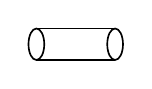
\begin{tikzpicture}[semithick, scale=0.5, baseline=-0.5ex] \begin{scope} \draw (-1,0) ellipse (0.2cm and 0.4cm); \draw (-1,0.4) -- (1,0.4); \draw (-1,-0.4) -- (1,-0.4); \draw (1,0) ellipse (0.2cm and 0.4cm); \end{scope} \end{tikzpicture}
        \quad
        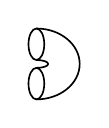
\begin{tikzpicture}[semithick, scale=0.5, baseline=-0.5ex] \begin{scope} \draw (0,0.5) ellipse (0.2cm and 0.4cm); \draw (0,-0.5) ellipse (0.2cm and 0.4cm); \draw (0,0.9) arc (90:-90:1.1cm and 0.9cm); \draw (0,0.1) arc (90:-90:0.3cm and 0.1cm); \end{scope} \end{tikzpicture}
        \quad
        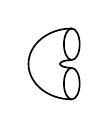
\begin{tikzpicture}[semithick, scale=0.5, baseline=-0.5ex] \begin{scope} \draw (0,0.5) ellipse (0.2cm and 0.4cm);\draw (0,-0.5) ellipse (0.2cm and 0.4cm); \draw (0,0.9) arc (90:270:1.1cm and 0.9cm); \draw (0,0.1) arc (90:270:0.3cm and 0.1cm); \end{scope} \end{tikzpicture}
        \quad
        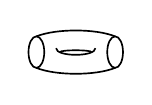
\begin{tikzpicture}[semithick, scale=0.5, baseline=-0.5ex] \begin{scope} \draw (-1,0) ellipse (0.2cm and 0.4cm); \draw (-1,0.4) .. controls (-0.5,0.6) and (0.5,0.6) .. (1,0.4); \draw (-1,-0.4) .. controls (-0.5,-0.6) and (0.5,-0.6) .. (1,-0.4); \draw (-0.5,0.1) .. controls (-0.5,-0.125) and (0.5,-0.125) .. (0.5,0.1); \draw (-0.4,0.0) .. controls (-0.4,0.0625) and (0.4,0.0625) .. (0.4,0.0); \draw (1,0) ellipse (0.2cm and 0.4cm); \end{scope} \end{tikzpicture}
        \quad
        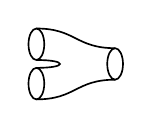
\begin{tikzpicture}[semithick, scale=0.5, baseline=-0.5ex] \begin{scope} \draw (-1,0.5) ellipse (0.2cm and 0.4cm); \draw (-1,-0.5) ellipse (0.2cm and 0.4cm); \draw (1,0) ellipse (0.2cm and 0.4cm); \draw (-1,0.9) .. controls (0,0.9) and (0,0.4) .. (1,0.4); \draw (-1,-0.9) .. controls (0,-0.9) and (0,-0.4) .. (1,-0.4); \draw (-1,0.1) .. controls (-0.2,0.1) and (-0.2,-0.1) .. (-1,-0.1); \end{scope} \end{tikzpicture}
        \quad
        
\begin{tikzpicture}[semithick, scale=0.5, baseline=-0.5ex] \begin{scope} \draw (-1,0) ellipse (0.2cm and 0.4cm); \draw (1,0.5) ellipse (0.2cm and 0.4cm); \draw (1,-0.5) ellipse (0.2cm and 0.4cm); \draw (-1,0.4) .. controls (0,0.4) and (0,0.9) .. (1,0.9); \draw (-1,-0.4) .. controls (0,-0.4) and (0,-0.9) .. (1,-0.9); \draw (1,0.1) .. controls (0.2,0.1) and (0.2,-0.1) .. (1,-0.1); \end{scope} \end{tikzpicture}
        \quad
        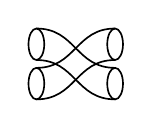
\begin{tikzpicture}[semithick, scale=0.5, baseline=-0.5ex] \begin{scope} \draw (-1,0.5) ellipse (0.2cm and 0.4cm); \draw (-1,-0.5) ellipse (0.2cm and 0.4cm); \draw (1,0.5) ellipse (0.2cm and 0.4cm); \draw (1,-0.5) ellipse (0.2cm and 0.4cm); \draw (-1,0.9) .. controls (0,0.9) and (0,-0.1) .. (1,-0.1); \draw (-1,0.1) .. controls (0,0.1) and (0,-0.9) .. (1,-0.9); \draw (-1,-0.9) .. controls (0,-0.9) and (0,0.1) .. (1,0.1); \draw (-1,-0.1) .. controls (0,-0.1) and (0,0.9) .. (1,0.9); \end{scope} \end{tikzpicture} \]
\end{example}

\begin{example}{bordism}
    Given bordisms $W : M \to M'$ and $W' : M' \to M''$, it can be shown that $W \sqcup_{M'} W'$ admits a smooth structure such that the inclusions $W \to W \sqcup_{M'} W'$ and $W' \to W \sqcup_{M'} W'$ are diffeomorphisms onto their images, which is unique up to (non-unique) diffeomorphism. Hence $W$ and $W'$ can be `composed' to produce a bordism $W' \circ W : M \to M''$, which is well-defined up to isomorphism.
    
    Using this composition rule, one can define the \textit{category of $n$-bordisms} $\textbf{Bord}_n$, where the objects are $(n - 1)$-dimensional closed manifolds and where the morphisms are bordsims are taken up to isomorphism. In particular, the identity morphism of an object $M$ is the cylinder $\id_M = M \times [0, 1]$.
\end{example}

\begin{topic}{lie-algebroid}{Lie algebroid}
    Let $M$ be a \tref{smooth-manifold}{smooth manifold}. A \textbf{Lie algebroid} over $M$ is a \tref{vector-bundle}{vector bundle} $L$ on $M$ together with a \tref{AA:lie-algebra}{Lie bracket} $[\cdot, \cdot]$ on its global sections $\Gamma(L)$ and a map of vector bundles $a : L \to TM$, called the \textit{anchor map}, to the \tref{tangent-bundle}{tangent bundle} of $M$, satisfying
    \begin{itemize}
        \item (\textit{Lie algebra homomorphism}) $a([X, Y]) = [a(X), a(Y)]$ for all $X, Y \in \Gamma(L)$,
        \item (\textit{Leibniz rule}) $[X, fY] = f[X, Y] + (a(X)  f) Y$ for all $X, Y \in \Gamma(L)$ and $f \in C^\infty(M)$.
    \end{itemize}
\end{topic}

\begin{example}{lie-algebroid}
    The tangent bundle $TM$ itself is a Lie algebroid, with the anchor map the identity $\id : TM \to TM$, and Lie bracket the \tref{lie-bracket-vector-fields}{Lie bracket for vector fields}.
\end{example}

\begin{example}{lie-algebroid}
    Given a vector bundle $E \to M$, its \textit{general linear algebroid} is the vector bundle $\mathfrak{gl}(E) \to M$ whose sections are derivations $D : \Gamma(E) \to \Gamma(E)$ of $E$ admitting a vector field $X_D \in TM$ such that $D(f s) = f D(s) + (X_D f) s$ for all $s \in \Gamma(E)$ and $f \in C^\infty(M)$. The Lie bracket is the commutator of differential operators, and the anchor map is the map $D \mapsto X_D$.
\end{example}

\begin{topic}{foliation}{foliation}
    Let $M$ be an $n$-dimensional \tref{smooth-manifold}{smooth manifold}. A $p$-dimensional \textbf{foliation} of $M$ is a decomposition of $M$ into a union of disjoint connected submanifolds
    \[ M = \bigsqcup_{\alpha \in A} L_\alpha \]
    such that each point $x \in M$ has a neighborhood $U$ with local coordinates $x^1, \ldots, x^n$ such that $x^{p + 1}, \ldots, x^n$ are constant on $U \cap L_\alpha$ for all $\alpha \in A$. The submanifolds $L_\alpha$ are called the \textbf{leaves} of the foliation, and the foliation is denoted as $\mathcal{F} = \{ L_\alpha \}_{\alpha \in A}$.
\end{topic}

\begin{topic}{higgs-bundle}{Higgs bundle}
    Let $M$ be a complex manifold. A \textbf{Higgs bundle} on $M$ is a holomorphic vector bundle $E$ on $M$ together with a section $\phi \in \Omega^1(M; \text{End}(E))$, called the \textbf{Higgs field}, satisfying $\phi \wedge \phi = 0$.
\end{topic}

\begin{topic}{frame-bundle}{(tangent) frame bundle}
    The \textbf{frame bundle} of a \tref{vector-bundle}{vector bundle} $E \to M$ of rank $k$ is the vector bundle $F(E) \to M$ whose fibers $F_x$ at a point $x \in M$ is the vector space of ordered bases $\{ e_1, \ldots, e_k \}$ of $E_x$.
    
    There is a natural fiber-wise action of $\text{GL}_k(\RR)$ on $F(E)$ given by change of basis: $\{ e_1, \ldots, e_k \} \cdot g = \{ f_1, \ldots, f_k \}$ where $f_i = \sum_j e_j g_{ji}$. This makes $F(E)$ into a \tref{TO:principal-bundle}{$\text{GL}_k(\RR)$-principal bundle}.
    
    When $E = TM$, the \tref{tangent-bundle}{tangent bundle}, the frame bundle $F(TM)$ is called the \textbf{tangent frame bundle}.
\end{topic}

\begin{topic}{spin-structure}{spin structure}
    Let $(M, g)$ be an $n$-dimensional orientable \tref{riemannian-manifold}{Riemannian manifold}. A \textbf{spin structure} on $M$ is a \tref{TO:principal-bundle}{principal $\text{Spin}(n)$-bundle} $P \to M$ together with a bundle morphism $f : P \to F_{\text{SO}(n)}(M)$ to the oriented orthonormal \tref{frame-bundle}{tangent frame bundle}, equivariant with respect to the double cover $\text{Spin}(n) \to \text{SO}(n)$.
    % Can be generalized to any vector bundle
\end{topic}

\begin{topic}{first-stiefel-whitney-class}{first Stiefel--Whitney class}
    Let $M$ be a \tref{smooth-manifold}{smooth manifold}. There exists a bijection between real line bundles $E \to M$ which can be trivialized over an open cover $\mathcal{U}$ and $\check{H}^1(M, C^\infty(M, \RR^*); \mathcal{U})$, in terms of the transition functions. The group isomorphism
    \[ C^\infty(M, \RR) \times \ZZ_2 \to C^\infty(M, \RR^*), \quad (f, \varepsilon) \mapsto \varepsilon e^f \]
    yields an isomorphism of \tref{AG:cech-cohomology}{Čech cohomology} groups
    \[ \check{H}^k(M; C^\infty(M, \RR); \mathcal{U}) \times \check{H}^k(M; \ZZ_2; \mathcal{U}) \to \check{H}^k(M; C^\infty(M, \RR^*); \mathcal{U}) , \]
    which for $k > 0$ specializes to an isomorphism
    \[ \check{H}^k(M; \ZZ_2; \mathcal{U}) \xrightarrow{\sim} \check{H}^k(M; C^\infty(M, \RR^*); \mathcal{U}) . \]
    The \textbf{first Stiefel--Whitney class} of a real line bundle $E \to M$ is its corresponding class $w_1(E) \in \check{H}^1(M; \ZZ_2; \mathcal{U})$.
    
    The \textbf{first Stiefel--Whitney class} of a rank $k$ real vector bundle $E \to M$ is the first Stiefel--Whitney class of $\wedge^k E$.
\end{topic}

\begin{topic}{first-chern-class}{first Chern class}
    Let $M$ be a \tref{smooth-manifold}{smooth manifold}. There exists a bijection between complex line bundles $E \to M$ which can be trivialized over an open cover $\mathcal{U}$ and $\check{H}^1(M, C^\infty(M, \CC^*); \mathcal{U})$, in terms of the transition functions. The exponential sequence
    \[ 0 \to \ZZ \xrightarrow{2 \pi i} C^\infty(M, \CC) \xrightarrow{\exp} C^\infty(M, \CC^*) \to 0 \]
    yields a long exact sequence of \tref{AG:cech-cohomology}{Čech cohomology} groups
    \[ \cdots \to \check{H}^k(M; \ZZ; \mathcal{U}) \to \check{H}^k(M; C^\infty(M, \CC); \mathcal{U}) \to \check{H}^k(M; C^\infty(M, \CC^*); \mathcal{U}) \to \check{H}^{k + 1}(M; \ZZ; \mathcal{U}) \to \cdots \]
    which in particular gives an isomorphism
    \[ \check{H}^1(M; C^\infty(M, \CC^*); \mathcal{U}) \xrightarrow{\sim} \check{H}^2(M; C^\infty(M, \ZZ; \mathcal{U}) . \]
    The \textbf{first Chern class} of a complex line bundle $E \to M$ is its corresponding class $c_1(E) \in \check{H}^2(M; \ZZ; \mathcal{U})$.
    
    The \textbf{first Chern class} of a rank $k$ complex vector bundle $E \to M$ is the first Chern class of $\wedge^k E$.
\end{topic}

\begin{topic}{determinant-bundle}{determinant bundle}
    The \textbf{determinant bundle} of a \tref{vector-bundle}{vector bundle} $E \to M$ of rank $k$ is the exterior power $\det(E) = \wedge^k E$.
\end{topic}

\begin{topic}{riemann-surface}{Riemann surface}
    A \textbf{Riemann surface} is a \tref{TO:connected-space}{connected} complex manifold of complex dimension one.
\end{topic}

\begin{topic}{volume-form}{volume form}
    Let $M$ be an $n$-dimensional \tref{smooth-manifold}{smooth manifold}. A \textbf{volume form} on $M$ is an \tref{differential-form}{$n$-form} $\omega \in \Omega^n(M)$.
\end{topic}

\begin{example}{volume-form}
    When $M$ is a \tref{riemannian-manifold}{Riemannian manifold} with metric $g$, there is a natural volume form on $M$. In local coordinates $x_1, \ldots, x_n$ it is given by
    \[ \text{vol}_g = \sqrt{|\det g|} \; dx_1 \wedge dx_2 \wedge \cdots \wedge dx_n , \]
    which is indeed independent of the choice of local coordinates.
\end{example}

\begin{topic}{hodge-star-operator}{Hodge star operator}
    Let $(M, g)$ be an $n$-dimensional \tref{riemannian-manifold}{Riemannian manifold}. The \textbf{Hodge star operators} are the maps
    \[ \star : \Omega^k(M) \to \Omega^{n - k}(M) \]
    for $0 \le k \le n$ defined by
    \[ \alpha \wedge \star \beta = g(\alpha, \beta) \text{vol}_g \]
    for all $\alpha, \beta \in \Omega^k(M)$, where $\text{vol}_g = \sqrt{|\det g|} \; dx_1 \wedge \cdots dx_n$ is the \tref{volume-form}{volume form} induced by $g$. Here $g$ is defined on $\Omega^k(M)$ by
    \[ g(\alpha, \beta) = \det\left(g(\alpha_i, \beta_j)\right)_{i, j = 1}^{k} \]
    for decomposable $\alpha = \alpha_1 \wedge \cdots \wedge \alpha_k$ and $\beta = \beta_1 \wedge \cdots \wedge \beta_k$ and extended linearly.
\end{topic}

\begin{topic}{hodge-inner-product}{Hodge inner product}
    Let $(M, g)$ be a \tref{riemannian-manifold}{Riemannian manifold}. The \textbf{Hodge inner product} is the (global) inner product on the de Rham spaces $\Omega^k(M)$ given by
    \[ (\alpha, \beta) = \int_X \alpha \wedge \star \beta = \int_X g(\alpha, \beta) \; \text{vol}_g \]
    for $\alpha, \beta \in \Omega^k(M)$, where $\star$ denotes the \tref{hodge-star-operator}{Hodge star operator}.
\end{topic}

\begin{topic}{de-rham-complex}{de Rham complex}
    Let $M$ be a \tref{smooth-manifold}{smooth manifold}. The \textbf{de Rham complex} of $M$ is the \tref{HA:chain-complex}{cochain complex}
    \[ 0 \to \Omega^0(M) \xrightarrow{d} \Omega^1(M) \xrightarrow{d} \Omega^2(M) \xrightarrow{d} \cdots \]
    where $\Omega^k(M)$ denotes the space of \tref{differential-form}{differential $k$-forms}, and $d$ the \tref{exterior-derivative}{exterior derivative}.
    
    The \textbf{de Rham cohomology groups} $H_\text{dR}^k(M)$ are the \tref{HA:homology-object}{cohomology groups} of $\Omega^\bdot(M)$.
\end{topic}

\begin{topic}{harmonic-form}{harmonic form}
    Let $(M, g)$ be an $n$-dimensional \tref{riemannian-manifold}{Riemannian manifold}. The \tref{exterior-derivative}{exterior derivative} $d : \Omega^k(M) \to \Omega^{k + 1}(M)$ has an adjoint $\delta = (-1)^{nk + 1} \star d \star : \Omega^k(M) \to \Omega^{k - 1}(M)$ with respect to the \tref{hodge-inner-product}{Hodge inner product}. That is,
    \[ (d \alpha, \beta) = (\alpha, \delta \beta) \quad \text{for all } \alpha \in \Omega^k(M) \text{ and } \beta \in \Omega^{k + 1}(M) . \]
    A differential form $\alpha \in \Omega^k(M)$ is \textbf{harmonic} if $\Delta \alpha = 0$, where $\Delta = d \delta + \delta d$ is the \textit{Laplacian operator}.
\end{topic}

\begin{topic}{holonomy-group}{holonomy group}
    Let $\pi : E \to M$ be a \tref{vector-bundle}{vector bundle} over a \tref{smooth-manifold}{smooth manifold} $M$, and $\nabla$ a \tref{connection}{connection} on $E$. By \tref{parallel-transport}{parallel transport}, any loop $\gamma : [0, 1] \to M$ based at a point $x \in M$ yields a linear invertible map $P_\gamma : E_x \to E_x$. The \textbf{holonomy group} of $\nabla$ based at $x$ is the group
    \[ \text{Hol}_x(\nabla) = \{ P_\gamma \in \text{GL}(E_x) : \gamma \text{ is a loop based at } x \} . \]
    The \textbf{restricted holonomy group} is the subgroup $\text{Hol}_x^0(\nabla)$ coming from contractible loops.
\end{topic}

\begin{topic}{implicit-function-theorem}{implicit function theorem}
    The \textbf{implicit function theorem} states that if $f : \RR^{n + m} \to \RR^m$ is a continuously differentiable function, and $p \in \RR^{n + m}$ a point with $f(p) = 0$ such that the Jacobian matrix $J_f = \left(\frac{\partial f_i}{\partial x_j}\right)_{i,j = n + 1}^{n + m}$ is invertible at $p$, then there exists an open set $U \subset \RR^n$ containing $(p_1, \ldots, p_n)$ and a continuously differentiable function $g : U \to \RR^m$ such that $g(p_1, \ldots, p_n) = (p_{n + 1}, \ldots, p_{m + n})$ and $f(y, g(y)) = 0$ for all $y \in U$.
\end{topic}

\begin{topic}{killing-vector-field}{Killing vector field}
    Let $(M, g)$ be a \tref{riemannian-manifold}{Riemannian manifold}. A \tref{vector-field}{vector field} $X$ on $M$ is a \textbf{Killing vector field} if it preserves the metric, i.e. $\mathcal{L}_X g = 0$, where $\mathcal{L}_X$ is the \tref{lie-derivative}{Lie derivative} with respect to $X$.
\end{topic}

\begin{topic}{schouten-nijenhuis-bracket}{Schouten--Nijenhuis bracket}
    The \textbf{Schouten--Nijenhuis bracket} is a unique extension of the \tref{lie-bracket-vector-fields}{Lie bracket of vector fields} to a graded bracket of multivector fields. It is defined by
    \[ \begin{aligned} {[}X_1 \wedge \cdots \wedge X_m, Y_1 \wedge \cdots \wedge Y_n{]} = \sum_{\substack{1 \le i \le m \\ 1 \le j \le n}} (-1)^{i + j} [X_i, X_j] &X_1 \wedge \cdots \wedge X_{i - 1} \wedge X_{i + 1} \wedge X_m \\ \wedge &Y_1 \wedge \cdots \wedge Y_{j - 1} \wedge Y_{j + 1} \wedge Y_n , \end{aligned} \]
    for \tref{vector-field}{vector fields} $X_i$ and $Y_j$, and by
    \[ [f, X_1 \wedge \cdots \wedge X_m] = -\iota_{df} X_1 \wedge \cdots \wedge X_m \]
    for a function $f$.
\end{topic}

\begin{topic}{courant-bracket}{Courant bracket}
    Let $M$ be a \tref{smooth-manifold}{smooth manifold}. The \textbf{Courant bracket} on $M$ is the skew-symmetric bracket on the \tref{generalized-tangent-bundle}{generalized tangent bundle} $TM \oplus T^*M$ given by
    \[ [X + \xi, Y + \eta] = [X, Y] + \mathcal{L}_X \eta - \mathcal{L}_Y \xi - \frac{1}{2} d \left(\iota_X \eta - \iota_Y \xi \right) , \]
    where $[X, Y]$ is the usual \tref{lie-bracket-vector-fields}{Lie bracket of vector fields}.
\end{topic}

\begin{topic}{courant-algebroid}{Courant algebroid}
    Let $M$ be a \tref{smooth-manifold}{smooth manifold}. A \textbf{Courant algebroid} over $M$ is a \tref{vector-bundle}{vector bundle} $E$ on $M$ together with a non-degenerate symmetric bilinear form $\langle \cdot, \cdot \rangle : \Gamma(E) \times \Gamma(E) \to \RR$, a skew-symmetric bracket $[\cdot, \cdot] : \Gamma(E) \times \Gamma(E) \to \Gamma(E)$ and a smooth bundle map $\pi : E \to TM$ called the \textit{anchor map}, satisfying
    \begin{itemize}
        \item (\textit{Respecting bracket}) $\pi([X, Y]) = [\pi(X), \pi(Y)]$,
        \item (\textit{Left Jacobi identity}) $[X, [Y, Z]] = [[X, Y], Z] + [Y, [X, Z]]$,
        \item (\textit{Leibniz rule}) $[X, fY] = f[X, X] + \rho(X)(f) Y$,
        \item (\textit{Self-adjoint}) $\pi(X) \langle Y, Z \rangle = \langle [X, Y], Z \rangle + \langle Y, [X, Z] \rangle$,
        \item (\textit{}) $[X, X] = \frac{1}{2} \mathcal{D} \langle X, X \rangle$,
    \end{itemize}
    where $\mathcal{D} : C^\infty(M) \to \Gamma(E)$ is the differential operator.
\end{topic}

\begin{example}{courant-algebroid}
    The bundle $E = TM \oplus T^*M$ together with the bilinear form
    \[ \langle X + \xi, Y + \eta \rangle = \xi(Y) + \eta(X) , \]
    the \tref{courant-bracket}{Courant bracket}, and the projection map $\pi : TM \oplus T^*M \to TM$ as anchor map, is a Courant algebroid, called the \textit{split Courant algebroid}.
\end{example}

\begin{topic}{dirac-structure}{Dirac structure}
    Let $M$ be a \tref{smooth-manifold}{smooth manifold}. An \textbf{almost Dirac structure} on $M$ is a subbundle $L \subset TM \oplus T^*M$ of the \tref{generalized-tangent-bundle}{generalized tangent bundle} of $M$, such that $L$ maximal isotropic with respect to symmetric bilinear form $\langle X + \xi, Y + \eta \rangle = \xi(Y) + \eta(X)$. If moreover $L$ is closed under the \tref{courant-bracket}{Courant bracket}, it is called \textit{integrable}, or simply a \textbf{Dirac structure}.
\end{topic}

% \begin{example}{dirac-structure}

% \end{example}

\begin{topic}{related-vector-fields}{related vector fields}
    Let $f : M \to N$ be a \tref{smooth-map}{smooth map} between \tref{smooth-manifold}{smooth manifolds}. Then vector fields $X$ on $M$ and $Y$ on $M$ are \textbf{$f$-related} if $Y_{f(x)} = (df)_x(X_x)$ for all $x \in M$.
\end{topic}

\begin{topic}{multivector-field}{multivector field}
    Let $M$ be a \tref{smooth-manifold}{smooth manifold}. A \textbf{multivector field} on $M$ is a section of the exterior algebra $\bigwedge^\bdot TM$.
\end{topic}

\begin{topic}{chern-class}{Chern class}
    Let $\pi : E \to M$ be a \tref{vector-bundle}{vector bundle} of rank $n$, and $\nabla$ a \tref{connection}{connection} on $E$ with \tref{curvature-connection}{curvature} $F_\nabla \in \Omega^2(M; \textup{End}(E))$. The \textbf{total Chern form} of $E$ is given by
    \[ C(E) = 1 + c_1(E) + \cdots + c_n(E) = \det \left(1 + \frac{F_\nabla}{2 \pi i} \right) , \]
    where $c_k(E) \in \Omega^{2k}(M)$ is the \textbf{$k$-th Chern form}. The Chern forms are \tref{closed-form}{closed}, and the cohomology class $[c_k(E)] \in H_\textup{dR}^{2k}(M)$ is called the \textbf{$k$-th Chern class} of $E$. These classes are independent on the choice of connection.
\end{topic}

\begin{topic}{chern-character}{Chern character}
    Let $\pi : E \to M$ be a \tref{vector-bundle}{vector bundle}, and $\nabla$ a \tref{connection}{connection} on $E$ with \tref{curvature-connection}{curvature} $F_\nabla \in \Omega^2(M; \textup{End}(E))$. The \textbf{Chern character} of $E$ is given by
    \[ \textup{ch}(E) = \operatorname{tr} \exp \left(\frac{F_\nabla}{2 \pi i} \right) = \sum_{k = 0}^{\infty} \frac{1}{k!} \operatorname{tr} \left(\frac{F_\nabla}{2 \pi i}\right)^k . \]
    The cohomology class $[\textup{ch}(E)] \in H_\textup{dR}^\bdot(M)$ is independent on the choice of connection.
    
    The Chern character satisfies
    \[ [\textup{ch}(E \oplus F)] = [\textup{ch}(E)] + [\textup{ch}(F) ] \quad \text{ and } \quad [\textup{ch}(E \otimes F)] = [\textup{ch}(E)] \cdot [\textup{ch}(F)] . \]
\end{topic}

\begin{topic}{flow-box-theorem}{flow box theorem}
    Let $M$ be a \tref{smooth-manifold}{smooth manifold} with a point $p \in M$, and $X$ a \tref{vector-field}{vector field} such that $X(p) \ne 0$. Then the \textbf{flow box theorem} states that there exist local coordinates $x^1, \ldots, x^n$ around $p$ such that $X = \frac{\partial}{\partial x^1}$.
    
    More generally, if $X_1, \ldots, X_k$ are pairwise commuting vector fields, that is $[X_i, X_j] = 0$ for all $i, j$, which are linearly independent at $p$, then there exist local coordinates $x^1, \ldots, x^n$ such that $X_i = \frac{\partial}{\partial x^i}$.
\end{topic}

\begin{topic}{dolbeault-operators}{Dolbeault operators}
    Let $M$ be a complex manifold. The space $\Omega^{p, q}(M)$ of $(p, q)$-forms is defined by
    \[ \Omega_X^{p, q} = \underbrace{\Omega^{1,0}(M) \wedge \cdots \wedge \Omega^{1,0}(M)}_{\text{$p$ times}} \;\; \wedge \;\; \underbrace{\Omega^{0,1}(M) \wedge \cdots \wedge \Omega^{0,1}(M)}_{\text{$q$ times}} , \]
    where
    \[ \Omega^{1,0}(M) = \left\{ \textstyle\sum_{i = 1}^{n} f_i dz^i \right\} \quad \textup{and} \quad \Omega^{0,1}(M) = \left\{ \textstyle\sum_{i = 1}^{n} g_i d \overline{z}^i \right\} , \]
    and where $z^1, \ldots, z^n$ are local coordinates. Note that these definitions are independent of the chosen coordinates. The \textbf{Dolbeault operators} are the operators
    \[ \partial : \Omega^{p, q}(M) \to \Omega^{p + 1, q}(M) \quad \textup{and} \quad \overline{\partial} : \Omega^{p, q}(M) \to \Omega^{p, q + 1}(M) \]
    given by
    \[ \partial = \sum_{j = 1}^{n} dz^j \wedge \frac{\partial}{\partial z^j} \quad \text{and} \quad \bar{\partial} = \sum_{j = 1}^{n} d\bar{z}^j \wedge \frac{\partial}{\partial \bar{z}^j} . \]
    They satisfy the properties
    \[ \partial + \bar{\partial} = d, \quad \partial^2 = \bar{\partial}^2 = \partial \bar{\partial} + \bar{\partial} \partial = 0 , \]
    where $d$ is the \tref{exterior-derivative}{exterior derivative}.
\end{topic}

\begin{topic}{poincare-lemma}{Poincaré lemma}
    The \textbf{Poincaré lemma} states that on a \tref{AT:contractible-space}{contractible} \tref{smooth-manifold}{smooth manifold} $M$, every \tref{closed-form}{closed $k$-form} is \tref{exact-form}{exact} for $k \ge 1$. In particular, the \tref{de-rham-complex}{de Rham cohomology groups} $H^k_\textup{dR}(M) = 0$ for all $k \ge 1$.
\end{topic}

\begin{topic}{serre-swan-theorem}{Serre--Swan theorem}
    Let $M$ be a \tref{TO:compact-space}{compact} \tref{smooth-manifold}{smooth manifold}. The \textbf{Serre--Swan theorem} states that for any \tref{vector-bundle}{vector bundle} $E \to M$, its global sections $\Gamma(E)$ are a \tref{CA:finitely-generated-module}{finitely generated} \tref{CA:projective-module}{projective} $C^\infty(M)$-module, and conversely that all such modules arise in this way.
    
    In fact, the \tref{CT:functor}{functor} $\Gamma$ yields an \tref{CT:equivalence-of-categories}{equivalence of categories} between the category of vector bundles over $M$ and the category of finitely generated projective $C^\infty(M)$-modules.
\end{topic}

\begin{topic}{todd-class}{Todd class}
    Let $\pi : E \to M$ be a \tref{vector-bundle}{vector bundle}, and $\nabla$ a \tref{connection}{connection} on $E$ with \tref{curvature-connection}{curvature} $F_\nabla \in \Omega^2(M; \textup{End}(E))$. The form
    \[ \det\left(\frac{F_\nabla / 2 \pi i}{\exp(F_\nabla / 2 \pi i) - 1}\right) \in \Omega^\bdot(M) \]
    is \tref{closed-form}{closed}, and its cohomology class $\textup{td}(E) \in H^\bdot_\textup{dR}(M)$, called the \textbf{Todd class} of $E$, is independent of the choice of connection.
    
    The Todd class is multiplicative in the sense that $\textup{td}(E \oplus F) = \textup{td}(E) \cdot \textup{td}(F)$.
\end{topic}

\begin{topic}{dolbeault-cohomology}{Dolbeault cohomology}
    Let $M$ be a complex smooth manifold, and consider the \tref{dolbeault-operators}{Dolbeault operator}
    \[ \overline{\partial} : \Omega^{p, q}(M) \to \Omega^{p, q + 1}(M) . \]
    Since $\overline{\partial}^2 = 0$, one can form the \tref{HA:chain-complex}{complex} $(\Omega^{p, \bdot}(M), \overline{\partial})$, and the corresponding \tref{HA:homology-object}{cohomology group} $H^{p, q}(M, \CC)$ is called the \textbf{$(p, q)$-th Dolbeault cohomology group}.
\end{topic}

\begin{topic}{frobenius-theorem}{Frobeniuw theorem}
    Let $M$ be a \tref{smooth-manifold}{smooth manifold}. \textbf{Frobenius theorem} states there is a one-to-one correspondence between \tref{foliation}{foliations} on $M$ and \tref{involutive-distribution}{involutive distributions} $\mathcal{D} \subset TM$. In particular, a foliation $\mathcal{F}$ corresponds to the involutive distribution $\mathcal{D} = T \mathcal{F}$, where $T_x \mathcal{F} = T_x L$ for any $x \in M$ with $L$ the leaf through $x$.
\end{topic}

\begin{topic}{legendre-transform}{Legendre transform}
    Let $V$ be a real \tref{LA:vector-space}{vector space} and $f : V \to \RR$ a smooth function which is \textit{super-linear}, that is, $\sup_{v \in V} \left(p(v) - f(v) \right) < \infty$ for all $p \in V^*$. Then the \textbf{Legendre transform} of $f$ is
    \[ f^* : V^* \to \RR, \quad p \mapsto \sup_{v \in V} \left(p(v) - f(v) \right) . \]
\end{topic}

\begin{example}{legendre-transform}
    Let $Q$ be a \tref{smooth-manifold}{smooth manifold} and $L \in C^\infty(TM)$ a smooth function on the \tref{tangent-bundle}{tangent bundle}. Assume $L$ is fiberwise super-linear, i.e. $L(q, -) : T_q M \to \RR$ is super-linear for all $q \in Q$. Then the Legendre transform of $L$ is
    \[ H : T^*M \to \RR, \qquad (q, p) \mapsto \left(L(q, -)\right)^*(p) . \]
    In physics, in particular classical mechanics, $L$ is the \textit{Lagrangian} for a mechanical system with configuration space $Q$, and the Legendre transform $H = L^*$ is the \textit{Hamiltonian} of the system.
\end{example}

\begin{example}{legendre-transform}
    Let $f : V \to \RR$ be given by $f(v) = \tfrac{1}{2} g(v, v)$, for some positive definite metric $g : V \times V \to \RR$. Given some fixed $p \in V^*$, we can find the supremum $\sup_{v \in V} \left(p(v) - \tfrac{1}{2} g(v, v)\right)$ by looking for extreme values. Setting
    \[ \partial_k \left( p_i v^i - \frac{1}{2} g_{ij} v^i v^j \right) = p_k - g_{ki} v^i \]
    equal to zero gives $v^i = g^{ik} p_k$, and thus
    \[ f^*(p) = p_i g^{ik} p_k - \frac{1}{2} g_{ij} g^{i k} p_k g^{j \ell} p_\ell = \frac{1}{2} g^{ik} p_i p_k , \]
    that is, $f^*(p) = g^*(p, p)$ where $g^* : V^* \times V^* \to \RR$ is the dual metric.
\end{example}

\begin{topic}{nijenhuis-tensor}{Nijenhuis tensor}
    Let $M$ be a \tref{smooth-manifold}{smooth manifold} and $A$ a \tref{tensor-field}{tensor field} of type $(1, 1)$, that is, a linear map of bundles $A : TM \to TM$. The \textbf{Nijenhuis tensor} of $A$ is a tensor field $N_A$ of type $(1, 2)$ given by
    \[ N_A(X, Y) = -A^2 [X, Y] + A([AX, Y] + [X, AY]) - [AX, AY] . \]
\end{topic}

\begin{example}{nijenhuis-tensor}
    The \textit{Newlander–Nirenberg theorem} states that an \tref{complex-manifold}{almost complex structure} $J$ is integrable if and only if $N_J = 0$.
\end{example}

\begin{topic}{normal-bundle}{normal bundle}
    Let $i : N \to M$ be an \tref{immersion}{immersion} of \tref{smooth-manifold}{smooth manifolds}. The \textbf{normal bundle} to $N$ in $M$ is the quotient bundle
    \[ T_{N/M} = i^* TM / TN . \]
\end{topic}

\begin{topic}{tubular-neighborhood}{tubular neighborhood (theorem)}
    Let $M$ be a \tref{smooth-manifold}{smooth manifold} and $N \subset M$ a smooth submanifold, and let $T_{N/M}$ be the \tref{normal-bundle}{normal bundle} to $N$ in $M$. The \textbf{tubular neighborhood theorem} states that there exists an open neighborhood $U \subset M$ of $N$, an open neighborhood $V \subset T_{N/M}$ of the zero section, and a \tref{diffeomorphism}{diffeomorphism} $\phi : U \to V$ extending this zero section.
    
    Such a neighborhood $U$ is called a \textbf{tubular neighborhood} of $N$ in $M$.
\end{topic}

\begin{topic}{riemannian-curvature-tensor}{Riemannian curvature tensor}
    Let $(M, g)$ be a \tref{riemannian-manifold}{Riemannian manifold}. The \textbf{Riemann curvature tensor} is the \tref{tensor-field}{$(1, 3)$-tensor field} given by
    \[ R(X, Y, Z) = \nabla_Y \nabla_X Z - \nabla_X \nabla_Y Z - \nabla_{[Y, X]} Z , \]
    where $\nabla$ is the \tref{levi-civita-connection}{Levi-Civita connection} and $[\cdot, \cdot]$ the \tref{lie-bracket-vector-fields}{Lie bracket of vector fields}.
\end{topic}

\begin{topic}{ricci-curvature}{Ricci curvature}
    Let $(M, g)$ be a \tref{riemannian-manifold}{Riemannian manifold}. The \textbf{Ricci curvature} is the \tref{tensor-field}{$(0, 2)$-tensor field} given by
    \[ \textup{Ric}(X, Z) = \operatorname{tr} \left( Y \mapsto R(X, Y, Z) \right), \]
    where $R$ is the \tref{riemannian-curvature-tensor}{Riemannian curvature tensor}.
\end{topic}

\begin{topic}{generalized-tangent-bundle}{generalized tangent bundle}
    Let $M$ be a \tref{smooth-manifold}{smooth manifold}. The \textbf{generalized tangent bundle} of $M$ is the direct sum $TM \oplus T^*M$ of the \tref{tangent-bundle}{tangent bundle} $TM$ and the \tref{cotangent-bundle}{cotangent bundle} $T^*M$.
    
    There is a natural symmetric bilinear form on the generalized tangent bundle, given by
    \[ \langle X + \xi, Y + \eta \rangle = \xi(Y) + \eta(X) , \]
    for $X + \xi, Y + \eta \in \Gamma(TM \oplus T^*M)$.
\end{topic}

\begin{topic}{dorfman-bracket}{Dorfman bracket}
    Let $M$ be a \tref{smooth-manifold}{smooth manifold}. The \textbf{Dorfman bracket} is the bracket $[\cdot, \cdot]$ on the \tref{generalized-tangent-bundle}{generalized tangent bundle} given by
    \[ [X + \xi, Y + \eta] = [X, Y] + \mathcal{L}_X \eta - \mathcal{L}_Y \xi + d \iota_Y \xi , \]
    for $X + \xi, Y + \eta \in \Gamma(TM \oplus T^*M)$, where $[X, Y]$ denotes the \tref{lie-bracket-vector-fields}{Lie bracket of vector fields}, and $\mathcal{L}$ the \tref{lie-derivative}{Lie derivative}.
\end{topic}

\begin{topic}{generalized-complex-structure}{generalized complex structure}
    Let $M$ be a \tref{smooth-manifold}{smooth manifold}. A \textbf{generalized almost complex structure} on $M$ is an endomorphism
    \[ \mathcal{J} : TM \oplus T^*M \to TM \oplus T^*M , \]
    of the \tref{generalized-tangent-bundle}{generalized tangent bundle} on $M$, such that
    \begin{itemize}
        \item (\textit{complex structure}) $\mathcal{J}^2 = -\id$,
        \item (\textit{symplectic structure}) $\mathcal{J}^* = -\mathcal{J}$.
    \end{itemize}
    A \textbf{generalized complex structure} on $M$ is a generalized almost complex structure which is \textit{integrable}, meaning its $+i$-eigenbundle $T_{0, 1} \subset (TM \oplus T^*M)_\CC$ is involutive with respect to the \tref{courant-bracket}{Courant bracket}.
\end{topic}

\begin{example}{generalized-complex-structure}
    A generalized complex structure generalizes both \tref{complex-manifold}{(almost) complex structures} and \tref{symplectic-manifold}{symplectic structures}. Namely, given an almost complex structure $J : TM \to TM$ and symplectic structure $\omega : TM \to T^*M$, the endomorphisms
    \[ \mathcal{J}_J = \begin{pmatrix} -J & 0 \\ 0 & J^* \end{pmatrix} \qquad \textup{and} \qquad \mathcal{J}_\omega = \begin{pmatrix} 0 & -\omega^{-1} \\ \omega & 0 \end{pmatrix} \]
    are both generalized complex structures.
\end{example}

\begin{topic}{orientable-manifold}{orientable manifold}
    An $n$-dimensional \tref{smooth-manifold}{smooth manifold} $M$ is \textbf{orientable} if there exists a nowhere vanishing \tref{differential-form}{$n$-form} $\omega \in \Omega^n(M)$. Such an $n$-form is called a \textit{volume form} on $M$.
    % An \textbf{oriented manifold} is a manifold $M$ together with a choice of volume form.
\end{topic}

\begin{example}{orientable-manifold}
    \begin{itemize}
        \item Euclidean space $\RR^n$ is orientable, with $\omega = dx^1 \wedge \cdots \wedge dx^n$ a volume form.
        \item The $n$-torus $\mathbb{T}^n = \RR^n / \ZZ^n$ is orientable, with $\omega = dx^1 \wedge \cdots \wedge dx^n$ a volume form.
        \item The Mobiüs strip is not orientable.
        \item The real projective plane $\RR P^2$ is not orientable.
    \end{itemize}
\end{example}

\begin{topic}{isometry}{(local) isometry}
    Let $(M, g)$ and $(M', g')$ be two \tref{riemannian-manifold}{Riemannian manifolds}. A \tref{smooth-map}{smooth map} $f : M \to M'$ is an \textbf{isometry} if it is a \tref{diffeomorphism}{diffeomorphism} and $f^*g' = g$.
    
    Such a map $f$ is a \textbf{local isometry} if it is a \tref{diffeomorphism}{local diffeomorphism} and $f^*g' = g$.
\end{topic}

\begin{example}{isometry}
    Every isometry is a local isometry, but not conversely. Namely, if $M = \RR^1$ and $M' = S^1 \subset \RR^2$ with the natural Euclidean metrics, then the map $\RR \to S^1$ given by $x \mapsto (\cos(x), \sin(x))$ is a local isometry, but not an isometry since it is not a diffeomorphism.
\end{example}

\begin{topic}{scalar-curvature}{scalar curvature}
    Let $(M, g)$ be a \tref{riemannian-manifold}{Riemannian manifold}. The \textbf{scalar curvature} $R$ of $M$ is the trace of the \tref{ricci-curvature}{Ricci curvature} $\textup{Ric}$ with respect to the metric $g$. In local coordinates,
    \[ R = g^{ij} \textup{Ric}_{ij} . \]
\end{topic}

\begin{topic}{einstein-tensor}{Einstein tensor}
    Let $(M, g)$ be a \tref{riemannian-manifold}{Riemannian manifold}. The \textbf{Einstein tensor} is the \tref{tensor-field}{$(0, 2)$-tensor field} on $M$ given by
    \[ G = \textup{Ric} - \frac{1}{2} R g , \]
    where $\textup{Ric}$ denotes the \tref{ricci-curvature}{Ricci curvature} and $R$ the \tref{scalar-curvature}{scalar curvature}.
\end{topic}

\begin{topic}{hyperkahler-manifold}{hyperkähler manifold}
    A \textbf{hyperkähler manifold} is a \tref{riemannian-manifold}{Riemannian manifold} $(M, g)$ with three \tref{complex-manifold}{complex structures} $I, J, K$ on $M$ satisfying the quaternionic relations
    \[ I^2 = J^2 = K^2 = IJK = -1 . \]
\end{topic}

\begin{topic}{hypercomplex-manifold}{hypercomplex manifold}
    A \textbf{hypercomplex manifold} is a \tref{smooth-manifold}{smooth manifold} $M$ with three \tref{complex-manifold}{complex structures} $I, J, K$ on $M$ satisfying the quaternionic relations
    \[ I^2 = J^2 = K^2 = IJK = -1 . \]
\end{topic}

\begin{topic}{stokes-theorem}{Stokes' theorem}
    Let $M$ be an $n$-dimensional oriented \tref{TO:compact-space}{compact} \tref{smooth-manifold}{smooth manifold} (possibly with boundary), and $\omega$ an \tref{differential-form}{$(n - 1)$-form}. Then \textbf{Stokes' theorem} states that
    \[ \int_M d \omega = \int_{\partial M} \omega , \]
    where $\partial M$ denotes the boundary of $M$.
\end{topic}

\begin{example}{stokes-theorem}
    For $M = [a, b]$ a closed interval on the real line, Stokes' theorem reduces to the \textit{fundamental theorem of calculus}: for any $F : [a, b] \to \RR$, we have
    \[ \int_a^b F'(x) dx = F(b) - F(a) . \]
\end{example}

\begin{topic}{teichmuller-space}{Teichmüller space}
    Let $\Sigma$ be a surface (a $2$-dimensional \tref{smooth-manifold}{smooth manifold}). The \textbf{Teichmüller space} $T(\Sigma)$ of $\Sigma$ is the space of equivalence classes of \tref{complex-manifold}{complex structures} on $\Sigma$, where two complex structures $I, J$ are \textit{equivalent} if there is a holomorphic \tref{diffeomorphism}{diffeomorphism} $f : (\Sigma, I) \to (\Sigma, J)$, \tref{TO:isotopy}{isotopic} to the identity on $\Sigma$.
\end{topic}

\begin{example}{teichmuller-space}
    \begin{itemize}
        \item The Teichmüller space of the $2$-sphere $S^2$ is a single point.
        \item The Teichmüller space of $\RR^2$ is two points.
        \item The Teichmüller space of the open annulus is the interval $[0, 1)$, where the complex structure associated to $\lambda \in [0, 1)$ is the Riemann surface $\{ z \in \CC : \lambda < |z| < \lambda^{-1} \}$.
        \item The Teichmüller space of the torus $\mathbb{T}^2 = \RR^2/\ZZ^2$ is the upper half-plane $\mathbb{H} = \{ z \in \CC : \operatorname{Im} z > 0 \}$, where the complex structure associated to $\tau \in \mathbb{H}$ is the Riemann surface $\CC / (\ZZ + \tau \ZZ)$, a complex elliptic curve.
    \end{itemize}
\end{example}

\begin{topic}{hopf-fibration}{Hopf fibration}
    The \textbf{Hopf fibration} is a non-trivial \tref{TO:fiber-bundle}{fiber bundle} over $S^2$ with fiber $S^1$, whose total space is $S^3$.
    \[ S^1 \hookrightarrow S^3 \to S^2 \]
    Identifying $S^3 \simeq \{ (z_0, z_1) \in \CC^2 : |z_0|^2 + |z_1|^2 = 1 \}$ and $S^2 \simeq \CC P^2$, the Hopf fibration is given by
    \[ S^3 \to S^2, \quad (z_0, z_1) \mapsto (z_0 : z_1) . \]
\end{topic}

\begin{topic}{hairy-ball-theorem}{hairy ball theorem}
    The \textbf{hairy ball theorem} states that no non-vanishing \tref{vector-field}{vector field} exists on the $2$-sphere $S^2$. More generally, no non-vanishing vector field exists on $S^{2n}$ for any $n \ge 1$.
\end{topic}

\begin{example}{hairy-ball-theorem}
    \begin{proof}
        Take $S^{2n} = \{ x \in \RR^{2n + 1} : |x|^{2n} = 1 \}$, and suppose that there exists a non-vanishing vector field $v$ on $S^{2n}$. Viewing $v(x) \in T_x S^{2n} \subset \RR^{2n + 1}$, we have $v(x) \perp x$, and after rescaling we can assume $v(x)$ has unit length. Now consider the homotopy
        \[ H : S^{2n} \times [0, 1] \to S^{2n}, \quad (x, t) \mapsto \cos(t) x + \sin(t) v(x) , \]
        and note that $H(-, 0) = \id_{S^{2n}}$, while $H(-, 1) = -\id_{S^{2n}}$. However, since $\id_{S^{2n}}$ has degree $1$ while the antipodal map $-\id_{S^{2n}}$ has degree $-1$, no such homotopy can exist, and thus no such vector field $v$ can exist.
    \end{proof}
\end{example}

\begin{topic}{symplectic-manifold}{symplectic manifold}
    Let $M$ be a \tref{smooth-manifold}{smooth manifold}. A \textbf{symplectic form} on $M$ is a \tref{closed-form}{closed} and non-degenerate \tref{differential-form}{$2$-form} $\omega$ on $M$. The pair $(M, \omega)$ is called a \textbf{symplectic manifold}.
\end{topic}

\begin{example}{symplectic-manifold}
    Let $M = \RR^{2n}$ with standard coordinates $q^1, \ldots, q^n, p_1, \ldots, p_n$. Then the $2$-form
    \[ \omega = \sum_{i = 1}^{n} d q^i \wedge d p_i , \]
    is a symplectic form, the \textit{standard symplectic form}.
    
    In fact, \tref{darboux-theorem}{Darboux's theorem} states that any symplectic manifold locally has this form.
\end{example}

\begin{topic}{symplectomorphism}{symplectomorphism}
    A \textbf{symplectomorphism} is a \tref{diffeomorphism}{diffeomorphism} $\varphi : M \to M'$ between \tref{symplectic-manifold}{symplectic manifolds} $(M, \omega)$ and $(M', \omega')$ satisfying $\varphi^* \omega' = \omega$.
\end{topic}

\begin{topic}{tautological-one-form}{tautological 1-form}
    Let $Q$ be a \tref{smooth-manifold}{smooth manifold}. The \textbf{tautological $1$-form} is the \tref{differential-form}{$1$-form} $\theta$ on the \tref{cotangent-bundle}{cotangent bundle} $T^*Q$ given by
    \[ \theta_x = p(d \pi_x) \quad \text{ for all } x = (q, p) \in T^*Q , \]
    where $\pi : T^*Q \to Q$ denotes the projection.
\end{topic}

\begin{example}{tautological-one-form}
    Take $Q = \RR^n$ so that $T^* Q \simeq \RR^{2n}$ with standard coordinates $q^1, p_1, \ldots, q^n, p_n$. Then the tautological $1$-form is given by
    \[ \theta = \sum_{i = 1}^{n} p_i dq^i . \]
\end{example}

\begin{topic}{canonical-symplectic-form}{canonical symplectic form}
    Let $Q$ be a \tref{smooth-manifold}{smooth manifold}. The \textbf{canonical symplectic form} is the \tref{symplectic-manifold}{symplectic form} $\omega$ on the \tref{cotangent-bundle}{cotangent bundle} $T^* Q$ given by
    \[ \omega = -d \theta , \]
    where $\theta$ is the \tref{tautological-one-form}{tautological $1$-form}.
\end{topic}

\begin{example}{canonical-symplectic-form}
    Take $Q = \RR^n$ so that $T^* Q \simeq \RR^{2n}$ with standard coordinates $q^1, p_1, \ldots, q^n, p_n$. Then the tautological $1$-form is given by
    \[ \theta = \sum_{i = 1}^{n} p_i dq^i , \]
    and thus the canonical symplectic form is given by
    \[ \omega = -d \theta = \sum_{i = 1}^{n} d q^i \wedge d p_i. \]
\end{example}

\begin{topic}{symplectic-vector-field}{symplectic vector field}
    Let $(M, \omega)$ be a \tref{symplectic-manifold}{symplectic manifold}. A \tref{vector-field}{vector field} $X$ on $M$ is called \textbf{symplectic} if the \tref{interior-product}{interior product}
    \[ \iota_X \omega = \omega(X, -) \]
    is \tref{closed-form}{closed}.
\end{topic}

\begin{example}{symplectic-vector-field}
    Every \tref{hamiltonian-vector-field}{Hamiltonian vector field} is symplectic, since every exact form is closed. The converse is however not true. Let $M$ be the $2n$-torus $\RR^{2n}/\ZZ^{2n}$ with the standard symplectic form
    \[ \omega = \sum_{i = 1}^{n} dp_i \wedge dq^i . \]
    Then the vector field $X$ on $M$ given by $X(x) = v$ for some constant non-zero $v \in \RR^{2n}$ (identifying $T_x M$ canonically with $\RR^{2n}$) is symplectic, but not Hamiltonian.
\end{example}

\begin{topic}{hamiltonian-vector-field}{Hamiltonian vector field}
    Let $(M, \omega)$ be a \tref{symplectic-manifold}{symplectic manifold}. Every smooth function $H : M \to \RR$ uniquely determines a \tref{vector-field}{vector field} $X_H$ satisfying
    \[ \omega(X_H, -) = dH . \]
    Such a vector field is called a \textbf{Hamiltonian vector field} with \textbf{Hamiltonian $H$}.
\end{topic}

\begin{example}{hamiltonian-vector-field}
    Let $M = \RR^{2n}$ with the standard symplectic form
    \[ \omega = \sum_{i = 1}^{n} dp_i \wedge dq^i . \]
    Then the Hamiltonian vector field with Hamiltonian $H$ has the form
    \[ X_H = \left(\frac{\partial H}{\partial p_i}, -\frac{\partial H}{\partial q^i} \right) . \]
\end{example}

\begin{topic}{symplectic-action}{symplectic action}
    Let $(M, \omega)$ be a \tref{symplectic-manifold}{symplectic manifold} and $G$ a \tref{lie-group}{Lie group} acting on $M$. The action is called \textbf{symplectic} if every element of $G$ acts by a \tref{symplectomorphism}{symplectomorphism}.
\end{topic}

\begin{topic}{fundamental-vector-field}{fundamental vector field}
    Let $M$ be a \tref{smooth-manifold}{smooth manifold}, $G$ a \tref{lie-group}{Lie group} acting on $M$ via $\varphi : G \times M \to M$. For any $\xi \in \mathfrak{g}$ in the Lie algebra of $G$, the \textbf{fundamental vector field} of $\xi$ is the \tref{vector-field}{vector field} on $M$ given by
    \[ X_\xi(p) = d(\varphi(-, p))(e) \xi \in T_p M . \]
    Alternatively, we have
    \[ X_\xi(p) = \frac{d}{d t}\Big|_{t = 0} \varphi(\exp(t \xi), p) . \]
\end{topic}

\begin{topic}{moment-map}{moment map}
    Let $(M, \omega)$ be a \tref{symplectic-manifold}{symplectic manifold} and $G$ a \tref{lie-group}{Lie group} with a \tref{symplectic-action}{symplectic action} on $M$. A \textbf{moment map} for the action is a smooth map $\mu : M \to \mathfrak{g}^*$ such that
    \[ d \langle \mu, \xi \rangle = \omega(X_\xi, -) \]
    for all $\xi \in \mathfrak{g}$, and such that $\mu$ is $G$-equivariant with respect to the \tref{adjoint-representation}{co-adjoint representation} of $G$, that is,
    \[ \mu(g \cdot p) = \text{Ad}_G^* (g) \mu(p) \]
    for all $p \in M$ and $g \in G$.
\end{topic}

\begin{topic}{hamiltonian-manifold}{Hamiltonian manifold}
    Let $(M, \omega)$ be a \tref{symplectic-manifold}{symplectic manifold} and $G$ a \tref{lie-group}{Lie group} with a \tref{symplectic-action}{symplectic action} $\varphi : G \times M \to M$ on $M$. The action is \textbf{Hamiltonian} if it admits a \tref{moment-map}{moment map}.
    
    The collection $(M, \omega, G, \varphi, \mu)$ is called a \textbf{Hamiltonian manifold}.
\end{topic}

\begin{topic}{marsden-weinstein-quotient}{Marsden--Weinstein quotient}
    Let $(M, \omega, G, \varphi, \mu)$ be a \tref{hamiltonian-manifold}{Hamiltonian manifold}, and assume $G$ acts \tref{GT:free-group-action}{freely} and \tref{GT:proper-group-action}{properly} on the zero-level set of the \tref{moment-map}{moment map} $\mu^{-1}(0) \subset M$. The \textbf{Marsden--Weinstein theorem} states that the orbit space
    \[ M \sslash G := \mu^{-1}(0) / G \]
    is a \tref{symplectic-manifold}{symplectic manifold} in a canonical way, called the \textbf{Marsden--Weinstein quotient} of $M$ by $G$. That is, there exists a unique symplectic form $\overline{\omega}$ on $M \sslash G$ which pulls back to the restriction of $\omega$ on $\mu^{-1}(0) / G$.
    
    Furthermore,
    \[ \dim(M \sslash G) = \dim M - 2 \dim G . \]
\end{topic}

\begin{topic}{poisson-manifold}{Poisson manifold}
    Let $M$ be a \tref{smooth-manifold}{smooth manifold}. A \textbf{Poisson structure} on $M$ is a bracket $\{ \cdot, \cdot \}$ on the algebra $C^\infty(M)$ of smooth functions making it into a \tref{AA:poisson-algebra}{Poisson algebra}. A \textbf{Poisson manifold} is a manifold with a Poisson structure.
\end{topic}

\begin{example}{poisson-manifold}
    Any \tref{symplectic-manifold}{symplectic manifold} $(M, \omega)$ gives rise to a Poisson manifold with bracket given by
    \[ \{ F, G \} = \omega(X_F, X_G) \]
    where $X_F$ is the \tref{hamiltonian-vector-field}{Hamiltonian vector field} of $F$.
    Indeed the Leibniz rule is satisfied as
    \[ \{ FG, H \} = d(FG) X_H = (F d G + G d F) X_H = F (d G X_H) + G (d F X_H) = F \{ G, H \} + G \{ F, H \} . \]
    Furthermore, the Jacobi identity can be shown from
    \[ \{ \{ F, G \}, H \} + \{ \{ G, H \}, F \} + \{ \{ H, F \}, G \} = -d \omega(X_F, X_G, X_H) \]
    and that $\omega$ is closed.
\end{example}

\begin{topic}{poisson-map}{Poisson map}
    A \textbf{Poisson map} is a \tref{smooth-map}{smooth map} $\phi : M \to N$ between \tref{poisson-manifold}{Poisson manifolds} such that the pullback
    \[ \phi^* : C^\infty(N) \to C^\infty(M), \quad f \mapsto f \circ \phi \]
    is a morphism of Poisson algebras.
\end{topic}

\begin{topic}{darboux-theorem}{Darboux's theorem}
    Let $(M, \omega)$ be a \tref{symplectic-manifold}{symplectic manifold}. \textbf{Darboux's theorem} states that around any point $x \in M$, there are local coordinates $q^1, \ldots, q^n, p_1, \ldots, p_n$ such that
    \[ \omega = dq^i \wedge dp_i . \]
\end{topic}

\begin{example}{darboux-theorem}
    \begin{proof}
        Locally around $x$, we can write $\omega = \frac{1}{2} \omega_{ij} dx^i \wedge dx^j$. Consider $\omega_0 = \frac{1}{2} \omega_{ij}(x) dx^i \wedge dx^1$, which is also a symplectic form in the same neighborhood of $x$. Moreover, for a sufficiently small neighborhood around $x$, we have a family of symplectic forms
        \[ \omega(t) = (1 - t) \omega_0 + t \omega , \quad t \in [0, 1] . \]
        Since $\omega - \omega_0$ is closed, using \tref{poincare-lemma}{Poincaré's lemma} we can locally around $x$ write $\dot{\omega}(t) = \omega - \omega_0 = - d \lambda$ for some $1$-form $\lambda$. Since $\omega - \omega_0$ vanishes at $x$, we may choose $\lambda$ to vanish at $x$ up to second order. Now let $X(t)$ be the vector field defined by $\iota_{X(t)} \omega(t) = \lambda$, and let $\varphi_t$ be the flow of $X(t)$ around $x_0$. Since $\varphi_t(x) = x$ for all $t \in [0, 1]$, the flow $\varphi_t$ exists on the whole interval $t \in [0, 1]$ sufficiently close to $x$. Now,
        \[ \frac{d}{dt} \varphi_t^* \omega(t) = \varphi_t^* \left(\frac{\partial \omega(t)}{\partial t} + \mathcal{L}_{X(t)} \omega(t) \right) = \varphi_t^* \left(\frac{\partial \omega(t)}{\partial t} + d(\iota_{X(t)} \omega(t)) \right) = \varphi_t^* \left( -d \lambda + d \lambda \right) = 0 , \]
        using the \tref{cartan-formula}{Cartan formula}. This implies that $\varphi_1^* \omega = \varphi_1^* \omega(1) = \varphi_0^* \omega(0) = \omega_0$, so $\varphi_1$ is the desired diffeomorphism. Finally, by a linear change of variables the form $\omega_0$ can be reduced to the canonical form.
    \end{proof}
\end{example}

\begin{topic}{moser-stability}{Moser's stability}
    \textbf{Moser's stability} states that for a \tref{closed-manifold}{closed} \tref{smooth-manifold}{smooth manifold} $M$ and a family of \tref{symplectic-manifold}{symplectic forms} $(\omega_t)_{t \in [0, 1]}$ on $M$ such that the \tref{de-rham-complex}{cohomology classes} $[\omega_t] \in H^2_{\textup{dR}}(M)$ are constant, there exists an isotopy $\varphi : M \times [0, 1] \to M$ such that $\varphi_t^* \omega_0 = \omega_t$ for all $t \in [0, 1]$.
\end{topic}

\begin{example}{moser-stability}
    \begin{proof}
        The proof is known as \textbf{Moser's trick}. Suppose there exists such an isotopy $\varphi$, and define a vector field $X_t = \frac{d \varphi}{d t} \circ \varphi_t^{-1}$. Then by \tref{cartan-formula}{Cartan's formula} and properties of the \tref{lie-derivative}{Lie derivative},
        \[ 0 = \frac{d}{dt} \left(\varphi_t^* \omega_t\right) = \varphi_t^* \left(\mathcal{L}_{X_t} \omega_t + \frac{d}{dt} \omega_t \right) = \varphi_t^* \left(d \iota_{X_t} \omega_t + \frac{d}{dt} \omega_t \right) \]
        so we obtain
        \[ d \iota_{X_t} \omega_t + \frac{d \omega_t}{dt} = d(\iota_{X_t} \omega_t + \alpha_t) = 0 , \]
        where $\frac{d \omega_t}{d t} = d \alpha_t$ for a family of 1-forms $\alpha_t$ since $[\omega_t]$ is constant. Now since $\omega_t$ is non-degenerate, we can integrate $\iota_{X_t} \omega_t + \alpha_t$ to obtain $X_t$, and let $\varphi_t$ be the flow of $X_t$.
    \end{proof}
\end{example}

\begin{topic}{casimir-function}{Casimir function}
    Let $(P, \{ \cdot, \cdot \})$ be a \tref{poisson-manifold}{Poisson manifold}. A function $f \in C^\infty(P)$ is called \textbf{Casimir} if the \tref{hamiltonian-vector-field}{Hamiltonian vector field} $X_f = \{ f, - \}$ is zero.
\end{topic}

\begin{topic}{symplectic-connection}{symplectic connection}
    Let $(M, \omega)$ be a \tref{symplectic-manifold}{symplectic manifold}. A \textbf{symplectic connection} on $M$ is a \tref{affine-connection}{affine connection} $\nabla$ which is \tref{torsion-connection}{torsion-free} and preserves the symplectic form, that is
    \[ (\nabla_Z \omega)(X, Y) = d(w(X, Y)) - \omega(\nabla_Z X, Y) - \omega(X, \nabla_Z Y) = 0 \]
    for any \tref{vector-field}{vector fields} $X, Y$ and $Z$.
\end{topic}

\begin{topic}{fubini-study-form}{Fubini--Study form}
    The \textbf{Fubini--study form} on $\CC \PP^n$ is the unique $2$-form $\omega_\textup{FS}$ on $\CC \PP^n$ such that
    \[ \pi^* \omega_\textup{FS} = \frac{i}{2} \partial \bar{\partial} \log (|\cdot|^2) , \]
    where $\pi : \CC^n \setminus \{ 0 \} \to \CC \PP^n$ is the projection map, $\partial$ and $\bar{\partial}$ are the \tref{dolbeault-operators}{Dolbeault operators}, and $|\cdot| : \CC^n \to \RR$ is the Euclidean norm. It is a \tref{symplectic-manifold}{symplectic form}.
\end{topic}

\begin{topic}{compatible-triple}{compatible triple}
    Let $M$ be a \tref{smooth-manifold}{smooth manifold}. A \textbf{compatible triple} on $M$ is a triple $(\omega, J, g)$, where $\omega$ is a \tref{symplectic-manifold}{symplectic form} on $M$, $J$ is an \tref{complex-manifold}{almost complex structure} on $M$, and $g$ is a \tref{riemannian-manifold}{Riemannian metric} on $M$, such that
    \[ g(X, Y) = \omega(X, J(Y)) \]
    for all \tref{vector-field}{vector fields} $X$ and $Y$ on $M$.
    % Given two out of the three structures of a compatible triple, the third structure can be obtained.
\end{topic}

\begin{example}{compatible-triple}
    Let $M = \CC^n$ with the standard Hermitian metric $h(-, -)$. Decomposing in real and imaginary parts, we have
    \[ h(u, v) = g(u, v) + i \omega(u, v) \]
    for some bilinear forms $g$ and $\omega$. Since $h(v, u) = \overline{h(u, v)}$, it follows that $g$ is symmetric and $\omega$ is skew-symmetric. Moreover, $g$ and $\omega$ are non-degenerate since $h$ is. In particular, $g$ is a Riemannian metric, and $\omega$ a symplectic form. Furthermore, multiplication by $i$ defines an almost complex structure $J$. Note that
    \[ g(u, Jv) + i \omega(u, Jv) = h(u, iv) = i h(u, v) = i g(u, v) - \omega(u, v) , \]
    from which follows that
    \[ g(u, v) = \omega(u, Jv) , \]
    that is, $(\omega, J, g)$ is a compatible triple.
\end{example}

\begin{topic}{weyl-bundle}{Weyl bundle}
    Let $(M, \omega)$ be a \tref{symplectic-manifold}{symplectic manifold}. The \textbf{Weyl bundle} on $M$ is the \tref{vector-bundle}{vector bundle}
    \[ W = \widehat{\textup{Sym}}(T^*M) , \]
    that is, the \tref{AA:completion}{completed} \tref{AA:symmetric-algebra}{symmetric algebra} of the \tref{cotangent-bundle}{cotangent bundle}.
    
    The \textbf{formal Weyl algebra} is the vector bundle
    \[ W_\hbar = \widehat{\textup{Sym}}(T^*M) \llbracket \hbar \rrbracket , \]
    where $\hbar$ is a formal parameter.
\end{topic}

\begin{topic}{moyal-weyl-product}{Moyal--Weyl product}
    Let $(M, \omega)$ be a \tref{symplectic-manifold}{symplectic manifold}. The \textbf{Moyal--Weyl product} is a non-commutative product on the sections of the \tref{weyl-bundle}{formal Weyl bundle} $W_\hbar$. In local coordinates, if $y^1, \ldots, y^{2n}$ is a basis for $T^*M$, the Moyal--Weyl product is given by
    \[ \begin{aligned}
        a \circ b
            &= \left. \exp \left(-\frac{i\hbar}{2} \omega^{ij} \frac{\partial}{\partial y^i} \frac{\partial}{\partial z^j}\right) a(y) b(z) \right|_{z = y} \\
            &= \sum_{k = 0}^{\infty} \left(-\frac{i\hbar}{2}\right)^k \frac{1}{k!} \omega^{i_1 j_1} \cdots \omega^{i_k j_k} \frac{\partial^k a}{\partial y^{i_1} \cdots \partial y^{i_k}} \frac{\partial^k b}{\partial y^{j_1} \cdots \partial y^{j_k}} ,
    \end{aligned} \]
    for sections $a, b \in \Gamma(W_\hbar)$.
\end{topic}

\begin{example}{moyal-weyl-product}
    The center of $\Gamma(W_\hbar)$ with respect to the Weyl product is $C^\infty(M)\llbracket \hbar \rrbracket$. Namely, if $a$ is in the center of $\Gamma(W_\hbar)$ and $b = y^k$ for some $k$, then
    \[ a \circ b = a y^k - \frac{i\hbar}{2} \omega^{ik} \frac{\partial a}{\partial y^i} \qquad \text{ and } \qquad b \circ a = a y^k - \frac{i\hbar}{2} \omega^{kj} \frac{\partial a}{\partial y^j} , \]
    so
    \[ 0 = a \circ b - b \circ a = - i \hbar \omega^{ik} \frac{\partial a}{\partial y^i} . \]
    Varying $k$, we find that $\frac{\partial a}{\partial y^i} = 0$ for all $i$, so $a \in C^\infty(M)\llbracket \hbar \rrbracket$. The converse inclusion is straightforward.
\end{example}

\begin{topic}{fedosov-manifold}{Fedosov manifold}
    A \textbf{Fedosov manifold} is a triple $(M, \omega, \nabla)$, where $(M, \omega)$ is a \tref{symplectic-manifold}{symplectic manifold} and $\nabla$ is a \tref{torsion-connection}{torsion-free} \tref{symplectic-connection}{symplectic connection} on $M$.
\end{topic}

\begin{example}{fedosov-manifold}
    Any symplectic manifold $(M, \omega)$ admits a torsion-free symplectic connection. Namely, by \tref{darboux-theorem}{Darboux's theorem}, there exists a covering of $M$ by \textit{Darboux charts}, which are open subsets of the standard symplectic space $\RR^{2n}$ with coordinates $q^1, \ldots, q^n, p_1, \ldots, p_n$ and symplectic form $\omega = \sum_{i = 1}^{n} dq^i \wedge dp_i$. On such a standard symplectic space, the \tref{exterior-derivative}{exterior derivative} $d$ is a torsion-free symplectic connection, and gluing these using a \tref{partition-of-unity}{partition of unity}, we obtain a global torsion-free symplectic connection on $M$.
\end{example}

\begin{topic}{lagrangian-submanifold}{Lagrangian submanifold}
    Let $(M, \omega)$ be a \tref{symplectic-manifold}{symplectic manifold}. A submanifold $L \subset M$ is \textbf{Lagrangian} if $T_p L \subset T_p M$ is a \tref{LA:lagrangian-subspace}{Lagrangian subspace} for each $p \in M$.
\end{topic}

\begin{example}{lagrangian-submanifold}
    For any smooth manifold $Q$, consider the cotangent bundle $T^*Q$ with the \tref{canonical-symplectic-form}{canonical symplectic form} $\omega$.
    \begin{itemize}
        \item Then the zero section of $T^*Q \to Q$ is a Lagrangian submanifold.
        \item The fibers of $T^*Q \to Q$ are Lagrangian submanifolds.
        \item Given a one-form $\alpha \in \Omega^1(Q)$, the graph $\Gamma_\alpha \subset T^*L$ is a Lagrangian submanifold if and only if $\alpha$ is closed.
    \end{itemize}
\end{example}

\begin{topic}{weinstein-lagrangian-neighborhood-theorem}{Weinstein's Lagrangian neighborhood theorem}
    Let $(M, \omega)$ be a \tref{symplectic-manifold}{symplectic manifold}, and $L \subset M$ a \tref{TO:compact-space}{compact} \tref{lagrangian-submanifold}{Lagrangian submanifold}. Then \textbf{Weinstein's Lagrangian neighborhood theorem} states that there exists a neighborhood $U$ of the zero section in $T^*L$, and a neighborhood $V$ of $L$ in $M$, and a \tref{symplectomorphism}{symplectomorphism} $\varphi : (V, \omega) \to (U, \omega_\textup{can})$, where $\omega_\textup{can}$ denotes the \tref{canonical-symplectic-form}{canonical symplectic form} on $T^*L$.
\end{topic}

% \begin{topic}{fukaya-category}{Fukaya category}
%     Let $(M, \omega)$ be a \tref{symplectic-manifold}{symplectic manifold}. The \textbf{Fukaya category} of $M$ is the \tref{CT:category}{category} whose objects are \tref{lagrangian-submanifold}{Lagrangian submanifolds} of $M$, and whose morphisms ...
% \end{topic}

\begin{topic}{formal-deformation-quantization}{formal deformation quantization}
    Let $(M, \omega)$ be a \tref{symplectic-manifold}{symplectic manifold}. A \textbf{formal deformation quantization} of $M$ is an associative product $\star$ on $Z = C^\infty(M) \llbracket \hbar \rrbracket$ (complex-valued functions), called a \textit{star product}, bilinear over $\CC \llbracket \hbar \rrbracket$, satisfying
    \begin{itemize}
        \item (\textit{formal deformation}) $a \star b \mod \hbar = ab$ for all $a, b \in Z$,
        \item (\textit{locality}) if $a, b \in Z$, then
        \[ a \star b = \sum_{k \ge 0} \hbar^k c_k , \]
        with $c_k$ depending only on $\partial^\alpha a_i \partial^\beta b_j$ for $i + j + |\alpha| + |\beta| \le k$.
        \item (\textit{correspondence principle}) if $a, b \in Z$, then
        \[ [a, b] = a \star b - b \star a = - i \hbar \{ a_0, b_0 \} + \mathcal{O}(\hbar^2) , \]
        where $\{ \cdot, \cdot \}$ denotes the Poisson bracket associated to $\omega$.
    \end{itemize}
\end{topic}
\begin{topic}{lie-group}{Lie group}
    A \textbf{Lie group} is a \tref{GT:group}{group} $G$ which is also a finite-dimensional \tref{smooth-manifold}{smooth manifold}, such that the multiplication map $G \times G \to G : (x, y) \mapsto xy$ and the inversion map $G \to G : x \mapsto x^{-1}$ are \tref{smooth-map}{smooth}.
\end{topic}

\begin{topic}{adjoint-representation}{(co)adjoint representation}
    The \textbf{adjoint representation} of a \tref{lie-group}{Lie group} $G$ is a \tref{RT:representation}{representation} onto its Lie algebra $\mathfrak{g} = T_e G$ given by
    \[ \text{Ad}_G : G \to \text{GL}(\mathfrak{g}), \quad g \mapsto \text{Ad}_g := d c_g(e) , \]
    where $c_g : G \to G, h \mapsto g h g^{-1}$ denotes the \tref{GT:conjugation}{conjugation} map.
    
    The \textbf{co-adjoint representation} $\text{Ad}_G^* : G \to \text{GL}(\mathfrak{g}^*)$ is the \tref{RT:dual-representation}{dual representation} of $\text{Ad}_G$.
    
    The \textbf{adjoint representation} of a \tref{AA:lie-algebra}{Lie algebra} $\mathfrak{g}$ is a representation onto itself, given by
    \[ \text{ad}_{\mathfrak{g}}: \mathfrak{g} \to \mathfrak{gl}(\mathfrak{g}), \quad X \mapsto [X, -] . \]
\end{topic}

\begin{topic}{killing-form}{Killing form}
    Let $\mathfrak{g}$ be a \tref{AA:lie-algebra}{Lie algebra} of finite dimension over a field $k$. The \textbf{Killing form} of $\mathfrak{g}$ is the symmetric bilinear form
    \[ B : \mathfrak{g} \times \mathfrak{g} \to k, \quad B(x, y) = \textup{tr}(\textup{ad}_{\mathfrak{g}}(x) \circ \textup{ad}_{\mathfrak{g}}(y)) \]
    where $\text{ad}_\mathfrak{g} : \mathfrak{g} \to \mathfrak{gl}(\mathfrak{g})$ is the \tref{adjoint-representation}{adjoint representation} of $\mathfrak{g}$.
\end{topic}

\begin{topic}{narasimhan-seshadri-theorem}{Narasimhan--Seshadri theorem}
    Let $\Sigma$ be a \tref{riemann-surface}{Riemann surface} and $K \subset \textup{U}(n)$ a \tref{LA:unitary-group}{unitary group}. The \textbf{Narasimhan--Seshadri theorem} states that there is a \tref{TO:homeomorphism}{homeomorphism}
    \[ \operatorname{Rep}(\pi_1(\Sigma), K) \cong \operatorname{Hol}^\textup{ss}_{\textup{deg} = 0}(\Sigma, K \otimes_\RR \CC) \]
    between the character variety $\operatorname{Rep}(\pi_1(\Sigma), K) = \Hom(\pi_1(\Sigma), K) / K$, parametrizing \tref{RT:representation}{representations} of the \tref{AT:fundamental-group}{fundamental group} of $\Sigma$ into $K$ up to conjugation by $K$, and the moduli space of \tref{AG:stable-vector-bundle}{semistable} \tref{holomorphic-vector-bundle}{holomorphic} \tref{vector-bundle}{vector bundles} of degree zero with \tref{TO:structure-group}{structure group} $K \otimes_\RR \CC$.
    
    Moreover, the stable points correspond to the \tref{RT:irreducible-representation}{irreducible representations}, restricted to which the correspondence becomes a \tref{diffeomorphism}{diffeomorphism}.
\end{topic}


\chapter{Algebraic Geometry}
\renewcommand{\cat}{AG}
\begin{topic}{sheaf}{sheaf}
    Let $X$ be a \tref{TO:topological-space}{topological space}. A \textbf{presheaf} $\mathcal{F}$ of abelian groups on $X$ consists of
    \begin{itemize}
        \item an abelian group $\mathcal{F}(U)$ for every open subset $U \subset X$,
        \item a morphism $r_{UV} : \mathcal{F}(U) \to \mathcal{F}(V)$ for every inclusion $V \subset U$ of open subsets of $X$,
    \end{itemize}
    such that
    \begin{itemize}
        \item $r_{UU}$ is the identity map for any open $U \subset X$,
        \item if $W \subset V \subset U$ are open subsets of $X$, then $r_{UW} = r_{VW} \circ r_{UV}$.
    \end{itemize}
    Elements of $\mathcal{F}(U)$ are called \textit{sections}. The maps $r_{UV}$ are thought of as restriction maps, and for this reason $r_{UV}(s)$ is often simply written as $s|_V$, for $s \in \mathcal{F}(V)$. One can similarly define a preseheaf of rings, sets, etc.
    
    A presheaf $\mathcal{F}$ is a \textbf{sheaf} if it moreover satisfies:
    \begin{itemize}
        \item for any open $U \subset X$ and open covering $\{ U_i \}$ of $U$, if $s \in \mathcal{F}(U)$ is such that $s|_{U_i} = 0$ for all $i$, then $s = 0$.
        \item for any open $U \subset X$ and open covering $\{ U_i \}$ of $U$, suppose we have elements $s_i \in \mathcal{F}(U_i)$ such that $s_i|{U_i \cap U_j} = s_j|_{U_i \cap U_j}$ for all $i, j$. Then there is an element $s \in \mathcal{F}(U)$ such that $s_i = s|_{U_i}$ for all $i$. (Note that uniqueness follows from the above condition.)
    \end{itemize}
    
    A morphism of presheaves $f : \mathcal{F} \to \mathcal{G}$ consists of a morphism of abelian groups $f(U) : \mathcal{F}(U) \to \mathcal{G}(U)$ for each open set $U$, such that for every inclusion $V \subset U$ the diagram
    \[ \begin{tikzcd} \mathcal{F}(U) \arrow{r}{f(U)} \arrow[swap]{d}{r_{UV}} & \mathcal{G}(U) \arrow{d}{r'_{UV}} \\ \mathcal{F}(V) \arrow{r}{f(V)} & \mathcal{G}(V) \end{tikzcd} \]
    commutes. A morphism of sheaves is a morphism of presheaves.
\end{topic}

\begin{topic}{constant-sheaf}{constant sheaf}
    Let $X$ be a topological space, and $A$ an abelian group. The \textbf{constant sheaf} $\underline{A}$ on $X$ determined by $A$ is the sheaf given by
    \[ \underline{A}(U) = \{ \textup{locally constant functions } U \to A \} , \]
    and the usual restriction maps. Note that for every connected open set $U$ we have $\underline{A}(U) \simeq A$, hence the name `constant sheaf'.
\end{topic}

\begin{topic}{stalk}{stalk}
    Let $\mathcal{F}$ be a \tref{sheaf}{presheaf} on a topological space $X$, and take a point $x \in X$. The \textbf{stalk} $\mathcal{F}_x$ of $\mathcal{F}$ at $x$ is defined as the direct limit of the groups $\mathcal{F}(U)$ for all open sets $U$ containing $x$, via the restriction maps.
\end{topic}

\begin{topic}{associated-sheaf}{associated sheaf}
    Given a \tref{sheaf}{presheaf} $\mathcal{F}$, there is a sheaf $\mathcal{F}^+$ and a morphism $\theta : \mathcal{F} \to \mathcal{F}^+$, with the property that for any sheaf $\mathcal{G}$ and morphism $f : \mathcal{F} \to \mathcal{G}$ there is a unique morphism $g : \mathcal{F}^+ \to \mathcal{G}$ such that $f = g \circ \theta$. The sheaf $\mathcal{F}^+$ is called the \textbf{sheaf associated} to the presheaf $\mathcal{F}$.
    \[ \begin{tikzcd} \mathcal{F} \arrow{rr}{f} \arrow[swap]{dr}{\theta} && \mathcal{G} \\ & \mathcal{F}^+ \arrow[swap,dashed]{ur}{g} & \end{tikzcd} \]
\end{topic}

\begin{topic}{direct-image-sheaf}{direct image sheaf}
    Let $f : X \to Y$ be a map of topological spaces, and let $\mathcal{F}$ be a \tref{sheaf}{sheaf} on $X$. The \textbf{direct image sheaf} $f_* \mathcal{F}$ on $Y$ is defined by
    \[ (f_* \mathcal{F})(V) = \mathcal{F}(f^{-1}(V)) \]
    for any open set $V \subset Y$ (indeed this presheaf is a sheaf).
    
    This construction yields the \textbf{direct image functor}
    \[ f_* : \textup{Sh}(X) \to \textup{Sh}(Y) . \]
    It is the \tref{CT:adjoint}{right adjoint} of the \tref{inverse-image-sheaf}{inverse image functor} $f^{-1}$.
\end{topic}

\begin{topic}{inverse-image-sheaf}{inverse image sheaf}
    Let $f : X \to Y$ be a map of topological spaces, and let $\mathcal{G}$ be a \tref{sheaf}{sheaf} on $Y$. The \textbf{inverse image sheaf} $f^
    {-1}\mathcal{G}$ on $X$ is defined as the \tref{associated-sheaf}{sheaf associated} to the presheaf given by $U \mapsto \lim_{V \supset f(U)} \mathcal{G}(V)$ for any open set $U \subset X$.
    
    This construction yields the \textbf{inverse image functor}
    \[ f^{-1} : \textup{Sh}(Y) \to \textup{Sh}(X) . \]
    It is the \tref{CT:adjoint}{left adjoint} of the \tref{direct-image-sheaf}{direct image functor} $f_*$.
\end{topic}

\begin{topic}{flasque-sheaf}{flasque sheaf}
    A \tref{sheaf}{sheaf} $\mathcal{F}$ on a topological space $X$ is called \textbf{flasque} if for every inclusion $V \subset U$ of open sets, the restriction map $\mathcal{F}(U) \to \mathcal{F}(V)$ is surjective.
\end{topic}

\begin{topic}{skyscraper-sheaf}{skyscraper sheaf}
    Let $X$ be a topological space, $A$ an abelian group, and take a point $x \in X$. The \textbf{skyscraper sheaf} $i_x(A)$ at $x$ with value $A$ is defined as
    \[ i_x(A) (U) = \left\{ \begin{array}{cl} A & \text{if } x \in U, \\ 0 & \text{otherwise.} \end{array} \right. \]
    The stalks of this sheaf are $A$ at any point in the closure of $x$, and zero elsewhere.
    
    Equivalently, it is the \tref{direct-image-sheaf}{direct image sheaf} $i_*(\underline{A})$ for $\underline{A}$ the \tref{constant-sheaf}{constant sheaf} determined by $A$ on the closure $\overline{\{ x \}}$ and $i : \overline{\{ x \}} \to X$ the inclusion.
\end{topic}

\begin{topic}{sheaf-hom}{sheaf hom}
    Let $\mathcal{F}$ and $\mathcal{G}$ be \tref{sheaf}{sheaves} of abelian groups on a topological space $X$. The \textbf{sheaf hom} of $\mathcal{F}$ and $\mathcal{G}$ is the sheaf $\underline{\Hom}(\mathcal{F}, \mathcal{G})$ given by
    \[ \underline{\Hom}(\mathcal{F}, \mathcal{G})(U) = \Hom(\mathcal{F}|_U, \mathcal{G}|_U) . \]
\end{topic}

% Defining schemes
\begin{topic}{ringed-space}{(locally) ringed space}
    A \textbf{ringed space} is a pair $(X, \mathcal{O}_X)$ consisting of a \tref{TO:topological-space}{topological space} $X$ and a \tref{sheaf}{sheaf} of rings $\mathcal{O}_X$ on $X$.
    
    A morphism of ringed spaces from $(X, \mathcal{O}_X)$ to $(Y, \mathcal{O}_Y)$ is a pair $(f, f^\#)$ of a continuous map $f : X \to Y$ and a map $f^\# : \mathcal{O}_Y \to f_* \mathcal{O}_X$ of sheaves of rings on $Y$.
    
    A ringed space $(X, \mathcal{O}_X)$ is a \textbf{locally ringed space} if for each point $x \in X$, the \tref{stalk}{stalk} $\mathcal{O}_{X,x}$ is a \tref{AA:local-ring}{local ring}.
    
    A morphism of locally ringed spaces is a morphism $(f, f^\#)$ of ringed spaces such that for each point $x \in X$ the induced map of local rings $f^\#_x : \mathcal{O}_{Y, f(x)} \to \mathcal{O}_{X, x}$ is a \textit{local morphism}, i.e. the pre-image of the maximal ideal of $\mathcal{O}_{X, x}$ is the maximal ideal of $\mathcal{O}_{Y, f(x)}$.
\end{topic}

\begin{topic}{spectrum-ring}{spectrum of a ring}
    Let $R$ be a \tref{AA:ring}{commutative ring}. The \textbf{spectrum} of $R$ is the \tref{ringed-space}{locally ringed space} $(X, \mathcal{O}_X)$ defined as follows.
    \begin{itemize}
        \item The topological space $X$ is the set of \tref{AA:prime-ideal}{prime ideals} of $R$, whose closed sets are given precisely by the sets $V(I) = \{ \textup{prime ideals } \mathfrak{p} \textup{ with } \mathfrak{p} \supset I \}$ for all ideals $I$ of $R$.
        \item The \tref{sheaf}{sheaf} of rings $\mathcal{O}_X$ is given as follows. For each open set $U \subset X$, $\mathcal{O}_X(U)$ is the set of functions $s : U \to \sqcup_{\mathfrak{p} \in U} R_\mathfrak{p}$ with $s(\mathfrak{p}) \in R_\mathfrak{p}$ for each $\mathfrak{p} \in U$, such that $s$ is locally a quotient of elements of $R$. This means that for each $\mathfrak{p} \in U$, there is a neighborhood $V \subset U$ of $\mathfrak{p}$, and elements $a, f \in R$ such that for each $\mathfrak{q} \in V$, $f \not\in \mathfrak{q}$ and $s(\mathfrak{q}) = a/f$ in $A_\mathfrak{q}$. The sets $\mathcal{O}_X(U)$ are indeed rings.
    \end{itemize}
    The spectrum of $R$ is denoted $\Spec R$.
\end{topic}

\begin{example}{spectrum-ring}
    While $\mathcal{O}_X(D_f) = R_f$ is a localization for \tref{principal-open-subset}{principal opens} $D_f = \{ \mathfrak{p} \in \Spec R \mid f \not\in \mathfrak{p} \}$, generally for open $U$ the ring $\mathcal{O}_X(U)$ need not be a localization of $R$.
    
    Namely, let $k$ be a field and consider $R = k[x, y, z, w] / (xy - zw)$, and let $U = D_y \cup D_z$. The elements $w/y \in R_y = \mathcal{O}_X(D_y)$ and $x/z \in R_z = \mathcal{O}_X(D_z)$ are equal in the localization $R_{yz} = \mathcal{O}_X(D_{yz})$, so they glue to an element $f \in \mathcal{O}_X(U)$. However, if $f = g/h$ for some $g, h \in R$, then we must have $h \in (y, z)$, but then $h$ vanishes somewhere on $U$.
\end{example}

\begin{topic}{scheme}{scheme}
    A \textbf{scheme} is a \tref{ringed-space}{locally ringed space} $(X, \mathcal{O}_X)$ in which every point has an open neighborhood $U$ such that $(U, \mathcal{O}_X|_U)$ is isomorphic to the \tref{spectrum-ring}{spectrum} of a \tref{AA:ring}{ring}. A morphism of schemes is a morphism of locally ringed spaces.
    
    One calls $X$ the \textit{underlying topological space}, and $\mathcal{O}_X$ its \textit{structure sheaf}.
\end{topic}

\begin{topic}{affine-scheme}{affine scheme}
    A \tref{scheme}{scheme} is \textbf{affine} if it is isomorphic to the \tref{spectrum-ring}{spectrum} of a \tref{AA:ring}{ring}.
\end{topic}

\begin{topic}{principal-open-subset}{principal open subset}
    A \textbf{principal open subset} of an \tref{affine-scheme}{affine scheme} $\Spec R$ is an open subset of the form
    \[ (\Spec R)_f = \{ \mathfrak{p} \in \Spec R : f \not\in \mathfrak{p} \} \]
    for some $f \in R$.
\end{topic}

% Scheme properties
\begin{topic}{reduced-scheme}{reduced scheme}
    A \tref{scheme}{scheme} $X$ is \textbf{reduced} if for every open subset $U \subset X$ the ring $\mathcal{O}_X(U)$ is \tref{AA:reduced-ring}{reduced}.
    
    Equivalently, this is the case if all stalks $\mathcal{O}_{X, x}$ are reduced.
\end{topic}

\begin{topic}{integral-scheme}{integral scheme}
    A \tref{scheme}{scheme} $X$ is \textbf{integral} if it is non-empty and for every non-empty open subset $U \subset X$ the ring $\mathcal{O}_X(U)$ is a \tref{AA:domain}{domain}.
    
    Equivalently, this is the case if $X$ is \tref{reduced-scheme}{reduced} and \tref{TO:irreducible-space}{irreducible}.
\end{topic}

\begin{topic}{noetherian-scheme}{(locally) noetherian scheme}
    A \tref{scheme}{scheme} $X$ is \textbf{locally noetherian} if it can be covered by open affine subsets $\Spec A_i$, where each $A_i$ is a \tref{AA:noetherian-ring}{noetherian ring}. It is \textbf{noetherian} if it is locally noetherian and \tref{quasi-compact-scheme}{quasi-compact}.
\end{topic}

\begin{topic}{finite-type}{(locally) of finite type}
    A morphism $f : X \to Y$ of \tref{scheme}{schemes} is \textbf{of finite type at $x \in X$} if there exist affine opens $U = \Spec A \subset X$ containing $x$ and $V = \Spec B \subset Y$ with $f(U) \subset V$ such that $A$ is a \tref{AA:finitely-generated-algebra}{finitely generated} $B$-algebra (via the induced map $B \to A$).
    
    The morphism $f$ is \textbf{locally of finite type} if it is of finite type at each $x \in X$, and it is \textbf{of finite type} if it is locally of finite type and \tref{quasi-compact-morphism}{quasi-compact}.
\end{topic}

\begin{topic}{finite-presentation}{(locally) of finite presentation}
    A morphism $f : X \to Y$ of \tref{scheme}{schemes} is \textbf{of finite presentation at $x \in X$} if there exists affine opens $U = \Spec A \subset X$ containing $x$ and $V = \Spec B \subset Y$ with $f(U) \subset V$ such that $A$ is a \tref{AA:finitely-presented-algebra}{finitely presented} $B$-algebra (via the induced map $B \to A$).
    
    The morphism $f$ is \textbf{locally of finite presentation} if it is of finite presentation at each $x \in X$, and it is \textbf{of finite presentation} if it is locally of finite presentation, \tref{quasi-compact-scheme}{quasi-compact}, and \tref{separated-morphism}{quasi-separated}.
\end{topic}

\begin{topic}{finite-morphism}{finite morphism}
    A morphism $f : X \to Y$ of \tref{scheme}{schemes} is \textbf{finite} if there exists a covering of $Y$ by open affine subsets $V_i = \Spec B_i$, such that for each $i$, $f^{-1}(V_i)$ is affine, equal to $\Spec A_i$, where $A_i$ is a $B_i$-algebra which is a \tref{AA:finitely-generated-module}{finitely generated} $B_i$-module.
\end{topic}

\begin{topic}{quasi-finite-morphism}{quasi-finite morphism}
    A morphism $f : X \to Y$ of \tref{scheme}{schemes} is \textbf{quasi-finite} if it is of \tref{finite-type}{finite type}, and every point $x \in X$ is isolated in its fiber $f^{-1}(f(x))$, i.e. every fiber is a discrete finite set.
\end{topic}

\begin{example}{quasi-finite-morphism}
    Every \tref{finite-morphism}{finite morphism} is quasi-finite, but the converse is not true. Namely, consider the immersion
    \[ i : \Spec \ZZ[\tfrac{1}{2}] \to \Spec \ZZ . \]
    Since $i$ is an open immersion, all fibers either consist of a single point or are empty. Furthermore, $i$ is of finite type as $\ZZ[\tfrac{1}{2}]$ is a finitely generated $\ZZ$-algebra, and $i$ is quasi-compact since the source and target are affine, hence $i$ is quasi-finite. However, $i$ is not finite since $\ZZ[\tfrac{1}{2}]$ is not finitely generated as a $\ZZ$-module.
\end{example}

\begin{topic}{open-immersion}{open immersion}
    An \textbf{open immersion} is a morphism $j : U \to X$ of \tref{scheme}{schemes} which induces an isomorphism of $U$ with an open subscheme of $X$.
\end{topic}

\begin{topic}{closed-immersion}{closed immersion}
    A \textbf{closed immersion} is a morphism $i : Z \to X$ of \tref{scheme}{schemes} such that $i$ induces a \tref{TO:homeomorphism}{homeomorphism} of the underlying space of $Z$ onto a closed subset of that of $X$, and furthermore the induced map $i^\# : \mathcal{O}_X \to i_*\mathcal{O}_Z$ of sheaves on $X$ is surjective.
\end{topic}

\begin{topic}{immersion}{immersion}
    An \textbf{immersion} is a morphism $Y \to X$ of \tref{scheme}{schemes} which factors as $j \circ i$, where $i$ is a \tref{closed-immersion}{closed immersion} and $j$ is an \tref{open-immersion}{open immersion}.
    \[ Y \xrightarrow{i} U \xrightarrow{j} X \]
\end{topic}

\begin{topic}{affine-morphism}{affine morphism}
    A morphism $f : X \to Y$ of \tref{scheme}{schemes} is \textbf{affine} if the inverse image of every affine open in $Y$ is an affine open of $X$. 
\end{topic}

\begin{example}{affine-morphism}
    \begin{itemize}
        \item Any morphism $f : \Spec(R) \to \Spec(S)$ between affine schemes is affine.
        \item The inclusion $\iota : \AA^2_k \setminus \{ (0, 0) \} \to \AA^2_k$ is not affine, since $\AA^2_k \setminus \{ (0, 0) \}$ is not affine.
        \item Let $Y_1 = Y_2 = \AA^2_k$, and let $Y$ be obtained by gluing $Y_1$ and $Y_2$ along $\AA^2_k \setminus \{ (0, 0) \}$. Then the inclusions $j_i : Y_i \to Y$ are not affine, since $j_1^{-1}(Y_2) = j_2^{-1}(Y_1) = \AA^2_k \setminus \{ (0, 0) \}$ is not affine.
    \end{itemize}
\end{example}

\begin{topic}{quasi-compact-morphism}{quasi-compact morphism}
    A morphism $f : X \to Y$ of \tref{scheme}{schemes} is \textbf{quasi-compact} if the inverse image of every \tref{TO:compact-space}{compact} open in $Y$ is compact in $X$.
\end{topic}

\begin{topic}{quasi-compact-scheme}{quasi-compact scheme}
    A \tref{scheme}{scheme} $X$ is \textbf{quasi-compact} if its underlying \tref{TO:topological-space}{topological space} is \tref{TO:compact-space}{compact}.
\end{topic}

\begin{example}{quasi-compact-scheme}
    Any affine scheme $X = \Spec R$ is quasi-compact. Since the standard opens form a basis for the topology on $X$, it suffices to consider an open cover of the form $X = \cup_{f \in S} X_f$ for some subset $S \subset R$. Note that $\{ X_f : f \in S \}$ covers $X$ $\iff$ no prime ideal of $R$ contains $S$ $\iff$ $1$ is contained in the ideal generated by $S$. In case of the latter, $1$ is also contained in the ideal generated by some finite $S' \subset S$, so $X = \cup_{f \in S'} X_f$ as well.
\end{example}

\begin{example}{quasi-compact-scheme}
    Let $X = \Spec k[x_1, x_2, \ldots]$ and let $U = X \setminus \{ (x_1, x_2, \ldots) \}$. Since $X$ is affine, it is quasi-compact. However, $U$ is not quasi-compact as the cover $\{ X_{x_i} : i = 1, 2, \ldots \}$ does not admit a finite subcover. Namely, any finite subset $\{ X_{x_{i_1}}, X_{x_{i_2}}, \ldots, X_{x_{i_n}} \}$ will not cover the prime ideal $(x_{i_1}, x_{i_2}, \ldots, x_{i_n})$.
\end{example}

\begin{topic}{normal-scheme}{normal scheme}
    A \tref{scheme}{scheme} $X$ is \textbf{normal} if all of its local rings $\mathcal{O}_{X,x}$ are \tref{AA:integral-closure}{integrally closed} \tref{AA:domain}{domains}.
    % Every scheme can be `normalized'.
\end{topic}

\begin{example}{normal-scheme}
    The cusp $C = \Spec k[x, y] / (x^3 - y^2)$ is not normal since $k[x, y] / (x^3 - y^2)$ is not integrally closed: the element $t = y/x$ is integral, as $t^2 = x$, but does not lie in $k[x, y] / (x^3 - y^2)$.
    
    Adding this element gives
    \[ \begin{aligned}
        k[x, y, y/x] / (x^3 - y^2) &\isom k[t] \\
        x &\mapsto t^2 \\
        y &\mapsto t^3
    \end{aligned} \]
    which is integrally closed. This is the \textit{normalization} of $C$
    \[ \AA_k^1 \to C, \quad t \mapsto (t^2, t^3) . \]
\end{example}

\begin{example}{normal-scheme}
    Let $k$ be a field with $\operatorname{char}(k) \ne 2$, and consider $X = \Spec k[x, y, z] / (z^2 - xy)$. To show $X$ is a normal scheme, we will prove the ring $R = k[x, y, z] / (z^2 - xy)$ is an integrally closed domain. First of all, $R$ is a domain because $z^2 - xy$ is irreducible in $k[x, y, z]$. Note that $K$, the field of fractions of $R$, is a field extension of $k(x, y)$ of degree $2$. Take any element $f = \alpha + \beta z \in K$, with $\alpha, \beta \in k(x, y)$, and assume $f$ is integral over $R$. If the minimal polynomial of $f$ over $R$ is linear, then $f \in R$ and we are done. Otherwise, note that $f$ satisfies $f^2 - 2 \alpha f + (\alpha - \beta^2 xy) = 0$, so that $X^2 - 2 \alpha X + (\alpha^2 - \beta^2 xy)$ must be the minimal polynomial of $f$ over $R$, and hence the coefficients $-2 \alpha$ and $\alpha^2 - \beta^2 xy$ lie in $R$. Since $2$ is invertible in $R$, it follows that $\alpha \in R$ and $\beta^2 xy \in R$. As $xy$ is squarefree, we must have $\beta \in R$, so $f = \alpha + \beta z \in R$, and we conclude that $R$ is integrally closed.
\end{example}

\begin{topic}{separated-scheme}{(quasi-)separated scheme}
    A \tref{scheme}{scheme} $X$ is \textbf{separated} if the morphism $X \to \Spec \ZZ$ is \tref{separated-morphism}{separated}.
    
    A scheme $X$ is \textbf{quasi-separated} if the morphism $X \to \Spec \ZZ$ is \tref{separated-morphism}{quasi-separated}.
\end{topic}

\begin{topic}{separated-morphism}{(quasi-)separated morphism}
    A morphism $f : X \to Y$ of \tref{scheme}{schemes} is \textbf{quasi-separated} if the diagonal $\Delta_{X/Y} : X \to X \times_Y X$ is quasi-compact, and it is \textbf{separated} if the diagonal $\Delta_{X/Y}$ is a closed immersion.
\end{topic}

\begin{example}{separated-morphism}
    Any morphism of affine schemes is separated. Namely, for any $f : \Spec A \to \Spec B$, the diagonal $\Delta$ corresponds to the ring map $A \otimes_B A \to A : a \otimes a' \mapsto aa'$, which is clearly surjective. In this way $A$ is seen as a quotient of $A \otimes_B A$, so $\Delta$ is a closed immersion.
\end{example}

\begin{example}{separated-morphism}
    Let $X$ be the affine line with two origins, that is, glue two copies of $\AA_k^1$ along $\AA_k^1 \setminus \{ 0 \}$. We claim that $X$ is not separated over $k$. Namely, consider the map $\AA^1_k \to X \times_k X$ obtained from the two different maps $\AA_k^1 \to X$. Then the inverse image of the diagonal is $\AA_k^1 \setminus \{ 0 \}$, which is not closed. Hence, the diagonal is not closed and $\Delta$ is not a closed immersion. However, $X$ can be shown to be quasi-separated over $k$.
\end{example}

\begin{example}{separated-morphism}
    Let $X_1 = X_2 = \Spec k[x_1, x_2, \ldots]$ and let $X = X_1 \cup X_2$ glued along the complement of $\{ (x_1, x_2, \ldots) \}$. Now $\Delta_{X/k}^{-1}(X_1 \times X_2) = \Spec k[x_1, x_2, \ldots] \setminus \{ (x_1, x_2, \ldots) \}$ is not \tref{quasi-compact-scheme}{quasi-compact}, although $X_1 \times X_2$ is. Therefore, $X \to \Spec k$ is not quasi-separated, and in particular not separated.
\end{example}

\begin{topic}{proper-morphism}{proper morphism}
    A morphism $f : X \to Y$ of \tref{scheme}{schemes} is \textbf{proper} if it is \tref{separated-morphism}{separated}, \tref{finite-type}{of finite type} and \tref{TO:universally-closed}{universally closed}.
\end{topic}

\begin{example}{proper-morphism}
    Any \tref{closed-immersion}{closed immersion} $i : Y \to X$ is proper. Indeed, the base change of a closed immersion is again a closed immersion, so $i$ is universally closed. Separatedness can be checked locally on the target: if $X = \Spec R$ then $Y = \Spec R / I$ for some ideal $I \subset R$, so $Y$ is also affine, and any morphism between affine schemes is separated. From this local expression of $X$ and $Y$ it is also clear $i$ is of finite type.
\end{example}

\begin{example}{proper-morphism}
    The morphism $\AA_k^1 \to \Spec k$ is not proper as it is not universally closed. Namely, the projection $\AA^1_k \times \AA^1_k \to \AA^1_k$ sends the closed set $\{ xy - 1 = 0 \}$ to $\AA^1_k \setminus \{ 0 \}$ and thus cannot be a closed mapping. However, the morphism is clearly of finite type, and also separated as the diagonal $\Delta : \AA^1_k \to \AA^1_k \times \AA^1_k$ is closed, it is given by $\{ x - y = 0 \}$.
\end{example}

\begin{example}{proper-morphism}
    Let $X$ be the affine line with double origin, i.e. two copies of $\AA^1$ glued along $\AA^1 \setminus \{ 0 \}$. Then $X \to \AA^1$ is of finite type and universally closed (the latter as $X_R \to \AA^1_R$ is closed for all rings $R$). However, $X \to \AA^1$ is not separated and hence not proper. For this we need to show $\Delta_{X / \AA^1} : X \to X \times_{\AA^1} X$ is not a closed immersion. Consider $\AA^1 \to X \times_{\AA^1} X$ induced from the two maps different maps $\AA^1 \to X$, and note that the inverse image of the diagonal is $\AA^1 \setminus \{ 0 \}$ which is not closed. Hence the diagonal is not closed.
\end{example}

\begin{topic}{projective-morphism}{(quasi-)projective morphism}
    A morphism $f : X \to Y$ of \tref{scheme}{schemes} is
    \begin{itemize}
        \item \textbf{projective} (\textit{in the sense of EGA}) if it factors as
        \[ X \xrightarrow{i} \PP(\mathcal{E}) \xrightarrow{\pi} Y \]
        for some \tref{coherent-sheaf}{quasi-coherent} finite type $\mathcal{O}_Y$-module $\mathcal{E}$, with $i$ a \tref{closed-immersion}{closed immersion} and $\pi$ the projection,
        \item \textbf{bundle-projective} if it factors as
        \[ X \xrightarrow{i} \PP(\mathcal{E}) \xrightarrow{\pi} Y \]
        for some finite locally free $\mathcal{O}_Y$-module $\mathcal{E}$, with $i$ a \tref{closed-immersion}{closed immersion} and $\pi$ the projection,
        \item \textbf{H-projective} (\textit{`H' standing for Hartshorne}) if it factors as
        \[ X \xrightarrow{i} \PP^n_Y \xrightarrow{\pi} Y , \]
        for some integer $n \ge 0$, with $i$ a closed immersion and $\pi$ the projection.
        \item \textbf{locally projective} if there exists an open covering $Y = \bigcup_i U_i$ such that $f^{-1}(U_i) \to U_i$ is projective for each $i$.
    \end{itemize}
    The morphism $f$ is \textbf{quasi-projective} if it factors as
    \[ X \xrightarrow{j} X' \xrightarrow{g} Y , \]
    with $j$ an \tref{open-immersion}{open immersion} and $g$ a projective morphism.
\end{topic}

\begin{example}{projective-morphism}
    There are implications
    \[ \textup{H-projective} \Rightarrow \textup{bundle-projective} \Rightarrow \textup{projective} \Rightarrow \textup{locally projective} \]
    but the converses do not hold.
    \begin{itemize}
        \item Let $k$ be a field. The obvious morphism $\bigsqcup_{n = 1}^{\infty} \PP^n_k \to \bigsqcup_{n = 1}^{\infty} \Spec k$ is bundle-projective but not H-projective.
        \item Let $X$ be the affine line over $k$ with infinitely many origins. The morphism $\bigsqcup_{n = 1}^{\infty} \PP^n_k \to X$ which sends $\PP^n_k$ to the $n$-th origin is projective but not bundle-projective.
        \item There are examples of morphisms which are locally projective but not projective.
    \end{itemize}
\end{example}

\begin{topic}{regular-scheme}{regular scheme}
    A \tref{scheme}{scheme} $X$ is \textbf{regular} if it is \tref{noetherian-scheme}{locally noetherian} and all of its stalks are \tref{AA:regular-ring}{regular local rings}.
\end{topic}

\begin{topic}{variety}{variety}
    A \textbf{variety} is a \tref{reduced-scheme}{reduced} \tref{separated-morphism}{separated} \tref{scheme}{scheme} of \tref{finite-type}{finite type} over a \tref{AA:field}{field} $k$.
\end{topic}

\begin{topic}{complete-variety}{complete variety}
    A \tref{variety}{variety} over $k$ is \textbf{complete} if it is \tref{proper-morphism}{proper} over $k$.
\end{topic}

\begin{topic}{geometrically-regular}{geometrically regular}
    Let $X$ be a \tref{noetherian-scheme}{locally noetherian} \tref{scheme}{scheme} over a field $k$. Then $X$ is \textbf{geometrically regular at $x \in X$} over $k$ if for every finitely generated field extension $k \subset k'$ and any $x' \in X_{k'}$ lying over $x$, the local ring $\mathcal{O}_{X_{k'}, x'}$ is \tref{AA:regular-ring}{regular}.
    
    The scheme $X$ is \textbf{geometrically regular} over $k$ if $X$ it is so at all points $x \in X$.
\end{topic}

\begin{topic}{smooth-morphism}{smooth morphism}
    A morphism $f : X \to Y$ of \tref{scheme}{schemes} is \textbf{smooth} if
    \begin{itemize}
        \item it is \tref{finite-presentation}{locally of finite presentation},
        \item it is \tref{flat-morphism}{flat},
        \item all the fibers $X_y$ are \tref{geometrically-regular}{geometrically regular} over the residue field $k(y)$.
    \end{itemize}
\end{topic}

\begin{example}{smooth-morphism}
    The natural map $\Spec k[x, y, t] / (xy - t) \to \Spec k[t]$ is not smooth since the fiber $X_0 = \{ xy = 0 \}$ over $t = 0$ is not geometrically regular.
\end{example}

\begin{topic}{unramified-morphism}{unramified morphism}
    A morphism $f : X \to Y$ of \tref{scheme}{schemes} is \textbf{unramified} if
    \begin{itemize}
        \item it is \tref{finite-type}{locally of finite type},
        \item the residue field $k(x)$ is a \tref{AA:separable-field-extension}{separable algebraic extension} of $k(f(x))$, for all $x \in X$,
        \item $f^\#(\mathfrak{m}_{f(x)}) \mathcal{O}_{X, x} = \mathfrak{m}_x$ for all $x \in X$.
    \end{itemize}
\end{topic}

\begin{topic}{etale-morphism}{étale morphism}
    A morphism $f : X \to Y$ of \tref{scheme}{schemes} is \textbf{étale} if it is \tref{flat-morphism}{flat}, \tref{unramified-morphism}{unramified} and \tref{finite-presentation}{locally of finite presentation}.
\end{topic}

\begin{topic}{formally-smooth}{formally smooth morphism}
    A morphism $f : X \to Y$ of \tref{scheme}{schemes} is \textbf{formally smooth} if for every ring $A$, ideal $I \subset A$ with $I^2 = 0$, and commutative diagram
    \[ \begin{tikzcd} \Spec A/I \arrow{r} \arrow{d} & X \arrow{d}{f} \\ \Spec A \arrow{r} \arrow[dashed]{ur} & Y \end{tikzcd} \]
    there exists a morphism $\Spec A \to X$ making the diagram commute.
\end{topic}

\begin{example}{formally-smooth}
    The variety $\Spec(k[x, y]/(xy))$ is not formally smooth over $\Spec(k)$. Namely, take $A = k[x, y] / (xy)^2$ and $I = (xy)$. Then there exists no morphism $k[x, y]/(xy) \to k[x, y]/(xy)^2$ completing the diagram.
\end{example}

\begin{topic}{formally-unramified}{formally unramified morphism}
    A morphism $f : X \to Y$ of \tref{scheme}{schemes} is \textbf{formally unramified} if for every ring $A$, ideal $I \subset A$ with $I^2 = 0$, and commutative diagram
    \[ \begin{tikzcd} \Spec A/I \arrow{r} \arrow{d} & X \arrow{d}{f} \\ \Spec A \arrow{r} \arrow[dashed]{ur} & Y \end{tikzcd} \]
    there is at most one morphism $\Spec A \to X$ making the diagram commute.
\end{topic}

\begin{example}{formally-unramified}
    The affine line $\AA^1_k = \Spec(k[x])$ is not formally unramified over $k$. Namely, take $A = k[\varepsilon] / (\varepsilon^2)$ and $I = (\varepsilon)$. Then for any $k[x] \to k[\varepsilon]/(\varepsilon) = k : x \mapsto x_0$ there exists a whole family of morphisms $k[x] \to k[t]/(t^2)$ completing the diagram: one can send $x \mapsto x_0 + \alpha t + (t^2)$ for any $\alpha \in k$.
\end{example}

\begin{topic}{formally-etale}{formally étale morphism}
    A morphism $f : X \to Y$ of \tref{scheme}{schemes} is \textbf{formally étale} if for every ring $A$, ideal $I \subset A$ with $I^2 = 0$, and commutative diagram
    \[ \begin{tikzcd} \Spec A/I \arrow{r} \arrow{d} & X \arrow{d}{f} \\ \Spec A \arrow{r} \arrow[dashed]{ur} & Y \end{tikzcd} \]
    there exists a unique morphism $\Spec A \to X$ making the diagram commute.
    
    That is, $f$ is formally étale if it is \tref{formally-smooth}{formally smooth} and \tref{formally-unramified}{formally unramified}.
\end{topic}

\begin{example}{formally-etale}
    Any \tref{etale-morphism}{étale morphism} is formally étale, but the converse does not hold. Namely, the morphism $f : \Spec k \to \Spec k[x_1, x_2, \ldots] / (x_1^2, x_2^2, \cdots)$ is easily checked to be formally étale. However, since $f$ is not \tref{finite-presentation}{locally of finite presentation}, it cannot be étale.
    
    A morphism is étale if and only if it is formally étale and locally of finite presentation.
\end{example}

\begin{topic}{flat-morphism}{flat morphism}
    A morphism $f : X \to Y$ of \tref{scheme}{schemes} is \textbf{flat} if for every $x \in X$, the local ring $\mathcal{O}_{X, x}$ is \tref{AA:flat-module}{flat} as an $\mathcal{O}_{Y, f(x)}$-module.
\end{topic}

\begin{example}{flat-morphism}
    The morphism $\Spec k[x, y, t] / (xy - t) \to \Spec k[t]$ is flat. This follows from $k[x, y, t] / (xy - t)$ being flat over $k[t]$, because it is a free $k[t]$-module:
    \[ k[x, y, t] / (xy - t) \isom k[t] \oplus \bigoplus_{i \ge 1} k[t] \cdot x^i \oplus \bigoplus_{i \ge 1} k[t] \cdot y^i \]
    However, the morphism
    \[ \Spec k[x, y, t] / (txy - t) \to \Spec k[t] \]
    is not flat. Namely, at the maximal ideal $(x, y, t)$, we have that $(k[x, y, t] / (txy - t))_{(x, y, t)}$ is not flat over $k[t]_{(t)}$, as tensoring the injective map $k[t]_{(t)} \xrightarrow{\cdot t} k[t]_{(t)}$ does not give an injective map: $t$ is a zero-divisor in $k[x, y, t] / (txy - t)$.
\end{example}

\begin{topic}{dominant-morphism}{dominant morphism}
    A morphism $f : X \to Y$ of \tref{scheme}{schemes} is \textbf{dominant} if the image of $f$ is a \tref{TO:dense-set}{dense} subset of $Y$.
\end{topic}

\begin{topic}{serre-duality}{Serre duality}
    Let $X$ be a \tref{smooth-morphism}{smooth} projective \tref{scheme}{scheme} of dimension $n$, and let $\omega_X$ be its \tref{canonical-sheaf}{canonical sheaf}. Then \textbf{Serre duality} states that for every coherent sheaf $\mathcal{F}$ on $X$ there is a natural isomorphism
    \[ H^i(X, \mathcal{F}^\vee \otimes \omega_X) \isom H^{n - i}(X, \mathcal{F})^\vee . \]
\end{topic}

\begin{topic}{picard-group}{Picard group}
    The \textbf{Picard group} $\textup{Pic}(X)$ of a \tref{scheme}{scheme} $X$ is the \tref{GT:abelian-group}{abelian group} of isomorphism classes of \tref{invertible-sheaf}{invertible sheaves} on $X$, where addition is given by the tensor product
    \[ [\mathcal{L}_1] + [\mathcal{L}_2] = [\mathcal{L}_1 \otimes \mathcal{L}_2] . \]
\end{topic}

\begin{example}{picard-group}
    A trivialization of an invertible sheaf $\mathcal{L}$ is given by an open cover $\{ U_i \}$ of $X$ such that $\mathcal{L}|_{U_i} = \mathcal{O}_{U_i} s_i$ for some non-vanishing sections $s_i \in \mathcal{O}_X(U_i)$. Then on overlaps $U_{ij} = U_i \cap U_j$ we have
    \[ s_i|_{U_{ij}} = g_{ij} s_j|_{U_{ij}} \]
    for some \textit{transition functions} $g_{ij} \in \mathcal{O}_X^*(U_i \cap U_j)$. These functions satisfy the \textit{cocycle condition}: $g_{ii} = 1$ and $g_{ij} g_{jk} g_{ki} = 1$ on $U_i \cap U_j \cap U_k$. Given another set of generators
    \[ s'_i = h_i s_i \]
    with $h_i \in \mathcal{O}_X^*(U_i)$, we find $g'_{ij} = h_i g_{ij} h_j^{-1}$. Hence, there is a natural isomorphism
    \[ \textup{Pic}(X) \isom \check{H}^1(X, \mathcal{O}_X^*) \isom H^1(X, \mathcal{O}_X^*) . \]
    Indeed this is a homomorphism since multiplying transition functions corresponds to the tensor product of the corresponding invertible sheaves.
\end{example}

\begin{example}{picard-group}
    For a \tref{AA:domain}{domain} $R$, the Picard group $\textup{Pic}(X)$ of $X = \Spec(R)$ is isomorphic to the \tref{AA:picard-group}{Picard group} $\textup{Pic}(R)$ of $R$.
    
    Namely, suppose $I$ is an invertible ideal with inverse $J$, that is $IJ = R$. Then $\sum_{i = 1}^{n} x_i y_i = 1$ for some $x_i \in I$ and $y_i \in J$, which induces $R$-module maps
    \[ \begin{aligned}
        f &: R^n \to I, \quad (r_i)_{i = 1}^{n} \mapsto \sum_{i = 1}^{n} r_i x_i , \\
        g &: I \to R^n, \quad x \mapsto (x y_i)_{i = 1}^{n} .
    \end{aligned} \]
    Since the composition $I \xrightarrow{g} R^n \xrightarrow{f} I$ is the identity, we find that $R^n \isom I \oplus \ker(f)$, which shows that $I$ is a finitely generated projective $R$-module, that is, a line bundle over $X$. In particular, any principal fractional ideal $I = fR$, with $f \in K^*$, is isomorphic to $R$ as an $R$-module, so the associated line bundle is trivial.
    
    This defines a map $\varphi : \textup{Pic}(R) \to \textup{Pic}(X)$. To see why this is a group homomorphism, let $I$ and $J$ be invertible ideals. Since $I$ is projective, the functor $I \otimes_R (-)$ is exact, so the map $I \otimes_R J \to I \otimes_R F \isom F$, given by $\sum_{i = 1}^{n} x_i \otimes y_i \mapsto \sum_{i = 1}^{n} x_i y_i$, is an injection. Hence, $I \otimes_R J$ is isomorphic to its image $IJ \subset F$.
    
    Injectivity of $\varphi$ follows because any invertible ideal $I$ isomorphic to $R$ as $R$-modules must be of the form $I = fR$ for some $f \in K^*$, and hence is principal. Surjectivity of $\varphi$ is shown as follows. Let $L$ be a line bundle over $X$, i.e. a finitely generated projective $R$-module of rank $1$. As $L$ is projective, the functor $L \otimes_R (-)$ is exact, which yields an inclusion $L = L \otimes_R R \subset L \otimes_R K \isom K$. Since $L$ is finitely generated, the image of $L$ inside $K$ is a fractional ideal $I$. To show it is invertible, let $J$ be the fractional ideal corresponding to the dual bundle $L^\vee = \Hom_R(L, R)$. Then, $R \isom L \otimes_R L^\vee \isom I \otimes_R J \isom IJ$, so $IJ = fR$ for some $f \in K^*$, and hence $I (f^{-1} J) = R$, so $I$ is indeed invertible.
\end{example}

\begin{topic}{picard-functor}{Picard functor}
    Let $f : X \to S$ be a \tref{scheme}{scheme} over $S$. The \textbf{absolute Picard functor} is the functor that assigns to any $T \to S$ the \tref{picard-group}{Picard group} $\textup{Pic}(X \times_S T)$,
    \[ \textup{Pic}_X : \textbf{Sch}/S \to \textbf{Ab}, \quad T \mapsto \textup{Pic}(X \times_S T) . \]
    The \textbf{relative Picard functor} is the functor
    \[ \textup{Pic}_{X/S} : \textbf{Sch}/S \to \textbf{Ab}, \quad T \mapsto \textup{Pic}(X \times_S T) / f_T^* \textup{Pic}(T) . \]
\end{topic}

\begin{example}{picard-functor}
    Note that the absolute Picard functor is generally not a \tref{sheaf}{sheaf}. Namely, it can happen that $X$ is a scheme with non-trivial line bundle $\mathcal{L}$, and $\{ U_i \}$ an open cover such that $\mathcal{L}|_{X \times_S U_i}$ is trivial for all $i$. For example, take $X = \PP^1_S$ with $\mathcal{L} = \mathcal{O}(1)$ and $U_1 = \AA^1_S, U_2 = \AA^1_S$ the usual affine charts. Hence, $\textup{Pic}$ is not a sheaf for the Zariski topology on $\textbf{Sch}/S$, and in particular is not \tref{CT:representable-functor}{representable}.
\end{example}

\begin{topic}{euler-sequence}{Euler sequence}
    Let $A$ be any ground ring. The \textbf{Euler sequence} is the following exact sequence of sheaves on $\PP_A^n$:
    \[ 0 \rightarrow \Omega^1_{\PP^n_A/A} \rightarrow \mathcal{O}_{\PP_A^n}(-1)^{\oplus n + 1} \rightarrow \mathcal{O}_{\PP_A^n} \rightarrow 0 , \]
    where the latter map is given by the map of graded $A$-modules
    \[ S(-1)^{\oplus n + 1} \to S : e_i \mapsto x_i \qquad \textup{ with } S = A[x_0, x_1, \ldots, x_n] . \]
    One can check on the affine patches that the kernel is isomorphic to the relative differential module.
\end{topic}

\begin{topic}{complete-intersection}{complete intersection}
    A \tref{variety}{variety} $X$ of dimension $r$ in projective space $\PP^n$ is a \textbf{complete intersection} if the corresponding ideal $I(X)$ can be generated by $n - r$ elements.
\end{topic}

\begin{example}{complete-intersection}
    The twisted cubic is not a complete intersection:
    \[ X = \textup{Proj}\left(\frac{k[x, y, z, w]}{(xw - yz, y^2 - xz, z^2 - yw)}\right) \subset \PP_k^3 \]
    Namely, its dimension is one, but its ideal cannot be generated by $3 - 1 = 2$ elements.
\end{example}

\begin{topic}{tangent-sheaf}{tangent sheaf}
    Let $X$ be a non-singular \tref{variety}{variety} over $k$. The \textbf{tangent sheaf} of $X$ is defined to be
    \[ \mathcal{T}_X = \mathcal{H}\textup{om}(\Omega_{X/k}, \mathcal{O}_X) . \]
\end{topic}

\begin{topic}{canonical-sheaf}{canonical sheaf}
    Let $X$ be a \tref{non-singular-variety}{non-singular} \tref{variety}{variety} over $k$ of dimension $n$. The \textbf{canonical sheaf} of $X$ is defined to be
    \[ \omega_X = \wedge^n \Omega_{X/k} . \]
\end{topic}

\begin{topic}{geometric-genus}{geometric genus}
    Let $X$ be a non-singular \tref{projective-variety}{projective variety} over $k$. Its \textbf{geometric genus} is defined as
    \[ p_g = \dim_k H^0(X, \omega_X) , \]
    where $\omega_X$ is the \tref{canonical-sheaf}{canonical sheaf} of $X$.
\end{topic}

\begin{topic}{normal-sheaf}{(co)normal sheaf}
    Let $X$ be a non-singular \tref{variety}{variety} over $k$, and $Y$ a non-singular closed irreducible subvariety defined by the sheaf of ideals $\mathcal{I}$. The \textbf{conormal sheaf} of $Y$ in $X$ is the sheaf
    \[ \mathcal{I}/\mathcal{I}^2 . \]
    Its dual
    \[ \mathcal{N}_{Y/X} = \mathcal{H}\textup{om}(\mathcal{I}/\mathcal{I}^2, \mathcal{O}_X) \]
    is called the \textbf{normal sheaf} of $Y$ in $X$. It is locally free of rank $r = \textup{codim}(Y)$.
\end{topic}

\begin{topic}{geometric-point}{geometric point}
    A \textbf{geometric point} of a \tref{scheme}{scheme} $X$ defined over a field $k$ is a morphism
    \[ \Spec \overline{k} \to X , \]
    where $\overline{k}$ denotes an \tref{AA:algebraic-closure}{algebraic closure} of $k$.
\end{topic}

\begin{topic}{fppf-covering}{fppf covering}
    An \textbf{fppf covering} of a \tref{scheme}{scheme} $X$ is a family of morphisms $\left\{ f_i : X_i \to X \right\}_{i \in I}$ that are all \tref{flat-morphism}{flat}, \tref{finite-presentation}{locally of finite presentation}, and jointly surjective, i.e. $X = \bigcup_{i \in I} f_i(X_i)$.
    
    `fppf' stands for \textit{fidèlement plat de présentation finie}.
\end{topic}

\begin{example}{fppf-covering}
    Any Zariski, étale, smooth or syntomic covering is an fppf covering.
\end{example}

\begin{example}{fppf-covering}
    Consider the following cover of the affine line $\AA^1_k$,
    \[ \left\{ \AA^1_k \setminus \{ 0 \} \to \AA^1_k, \qquad \Spec(\mathcal{O}_{\AA^1_k, 0}) \to \AA^1_k \right\} . \]
    It is not an fppf covering since the second morphism is not locally of finite presentation.
    
    (However, it is an \tref{fpqc-covering}{fpqc covering}.)
\end{example}

\begin{topic}{fpqc-covering}{fpqc covering}
    An \textbf{fpqc covering} of a \tref{scheme}{scheme} $X$ is a family of morphisms $\left\{ f_i : X_i \to X \right\}_{i \in I}$ that are all \tref{flat-morphism}{flat}, and such that for every affine open $U \subset X$ there exists a finite subset $J \subset I$ and affine opens $V_j \subset X_j$ for each $j \in J$ such that $U = \bigcup_{j \in J} f_j(V_j)$. That is, every affine open in $X$ can be covered by finitely many affine opens from the $X_i$.
    
    `fpqc' stands for \textit{fidèlement plat et quasi-compact}.
\end{topic}

\begin{example}{fpqc-covering}
    Any \tref{fppf-covering}{fppf covering} $\{ f_i : X_i \to X \}_{i \in I}$ is an fpqc covering. By assumption the $f_i$ are flat. Let $U \subset X$ be an affine open. Write $f_i^{-1}(U) = \cup_{j \in J_i} U_{ij}$ for some affine opens $U_{ij} \subset X_i$. Each $f_i$ flat and locally of finite presentation, hence open. So, $U = \cup_{i \in I} \cup_{j \in J_i} f_i(U_{ij})$ is an open cover for $U$. Now, $U$ is affine and thus quasi-compact, so there is a finite subcover.
\end{example}

\begin{example}{fpqc-covering}
    A morphism $\Spec A \to \Spec B$ is an fpqc covering if and only if $A \to B$ is faithfully flat.
\end{example}

\begin{example}{fpqc-covering}
    Let $X = \AA^1_k$ be the affine line over an infinite field $k$, and consider the natural morphism
    \[ f : \bigsqcup_{x \in X} \Spec(\mathcal{O}_{X, x}) \to X . \]
    Altough it is flat and surjective, it does not define an fpqc covering of $X$, since any affine open of $\bigsqcup_{x \in X} \Spec(\mathcal{O}_{X, x})$ can only consist of finitely many points (because affines are quasi-compact).
\end{example}

\begin{topic}{faithfully-flat-morphism}{faithfully flat morphism}
    A morphism $f : X \to Y$ of \tref{scheme}{schemes} is \textbf{faithfully flat} if it is both \tref{flat-morphism}{flat} and surjective.
\end{topic}

\begin{topic}{big-small-site}{big/small site}
    Let $X$ be a \tref{scheme}{scheme}, and let $\tau$ be any of the properties in $\{$ Zariski, étale, smooth, fppf, fpqc $\}$.
    
    The \textbf{big $\tau$-site} of $X$ is the \tref{CT:site}{site} $(\textbf{Sch}/X)_\tau$ of schemes over $X$ with the $\tau$-topology.
    
    The \textbf{small $\tau$-site} of $X$ is the full subcategory $X_\tau$ of $(\textbf{Sch}/X)_\tau$ whose objects are schemes $T$ over $X$ whose structure morphism $T \to X$ is part of a $\tau$-covering.
\end{topic}

\begin{topic}{projection-formula}{projection formula}
    Let $f : X \to Y$ be a morphism of \tref{scheme}{schemes}, $\mathcal{F}$ an $\mathcal{O}_X$-module, and $\mathcal{E}$ a \tref{free-sheaf}{locally free} $\mathcal{O}_Y$-module. The \textbf{projection formula} states a natural isomorphism
    \[ f_*\left(\mathcal{F} \otimes_{\mathcal{O}_X} f^* \mathcal{E} \right) \isom f_*\left(\mathcal{F}\right) \otimes_{\mathcal{O}_Y} \mathcal{E} . \]
\end{topic}

\begin{topic}{rational-map}{rational map}
    A \textbf{rational map} $f : X \dashrightarrow Y$ between (\tref{TO:irreducible-space}{irreducible}) \tref{variety}{varieties} $X$ and $Y$ is an equivalence class of pairs $(U, f_U)$, where $U \subset X$ open and non-empty, $f_U : U \to Y$ a morphism, and where two pairs $(U, f_U)$ and $(V, f_V)$ are equivalent if their restriction to $U \cap V$ coincides.
\end{topic}

\begin{topic}{birational-map}{birational map}
    A \textbf{birational map} between (\tref{TO:irreducible-space}{irreducible}) \tref{variety}{varieties} $X$ and $Y$ is a \tref{rational-map}{rational map} $f : X \dashrightarrow Y$ which has a rational inverse. That is, there exists a rational map $g : Y \dashrightarrow X$ such that $gf = \id_X$ and $fg = \id_Y$ as rational maps.
    
    If there is a birational map from $X$ to $Y$, then $X$ and $Y$ are called \textbf{birationally equivalent}, or simply \textbf{birational}.
    
    A \textbf{birational morphism} is a morphism of varieties which has a rational inverse.
\end{topic}

\begin{example}{birational-map}
    The circle $X = \{ x^2 + y^2 = 1 \}$ in the affine plane is birational to the affine line $\AA^1$, since the rational map
    \[ f : \AA^1 \dashrightarrow X, \quad t \mapsto \left(\frac{2t}{1 + t^2}, \frac{1 - t^2}{1 + t^2}\right) \]
    has a rational inverse
    \[ g : X \dashrightarrow \AA^1, \quad (x, y) \mapsto \frac{1 - y}{x} . \]
\end{example}

\begin{example}{birational-map}
    Affine space $\AA^n$ is birational to projective space $\PP^n$ since the inclusion
    \[ i : \AA^n \to \PP^n, \quad (x_1, x_2, \ldots, x_n) \mapsto (1 : x_1 : \cdots : x_n) \]
    has rational inverse
    \[ j : \PP^n \dashrightarrow \AA^n, \quad (X_0 : X_1 : \cdots : X_n) \mapsto \left(\frac{X_1}{X_0}, \frac{X_2}{X_0}, \cdots, \frac{X_n}{X_0}\right) . \]
\end{example}

\begin{topic}{rational-variety}{rational variety}
    A \tref{variety}{variety} is called \textbf{rational} if it is \tref{birational-map}{birationally equivalent} to affine space (or equivalently, to projective space) of some dimension.
\end{topic}

\begin{topic}{syntomic-morphism}{syntomic morphism}
    A morphism $f : X \to Y$ of \tref{scheme}{schemes} is \textbf{syntomic at $x \in X$} if there exists an affine open neighborhood $U = \Spec A \subset X$ of $x$ and an affine open $V = \Spec B \subset Y$ with $f(U) \subset V$ such that the induced ring morphism $B \to A$ is \textit{syntomic}, i.e. of \tref{AA:finitely-presented-algebra}{finite presentation}, makes $A$ into a \tref{AA:flat-module}{flat} \tref{AA:module}{$B$-module}, and all the fiber rings $A \otimes_B k(\mathfrak{p})$ are local complete intersections.
    
    The morphism $f$ is \textbf{syntomic} if it is syntomic at all points $x \in X$.
\end{topic}

\begin{topic}{galois-cover}{Galois cover}
    A morphism $f : X \to S$ of \tref{scheme}{schemes} is a \textbf{Galois cover} if it is \tref{finite-morphism}{finite}, \tref{faithfully-flat-morphism}{faithfully flat}, and such that there exists a finite group $\Gamma$ of $S$-automorphisms, such that
    \[ \Gamma \times X \to X \times_S X, \quad (\sigma, x) \mapsto (x, \sigma(x)) \]
    is an isomorphism.
\end{topic}

\begin{example}{galois-cover}
    Let $\ell / k$ be a \tref{AA:galois-extension}{Galois extension} with \tref{AA:galois-group}{Galois group} $G = \textup{Gal}(\ell/k)$. Then there is an isomorphism
    \[ \ell \otimes_k \ell \to \prod_{\sigma \in G} \ell, \quad a \otimes b \mapsto (a \sigma(b))_{\sigma \in G} \]
    which shows that
    \[ G \times \Spec(\ell) \to \Spec(\ell) \times_{\Spec(k)} \Spec(\ell) \]
    is an isomorphism, and thus $\Spec(\ell) \to \Spec(k)$ is a Galois cover.
\end{example}

\begin{example}{galois-cover}
    Let $n \ge 1$ and let $k$ be a field containing a primitive $n$-th root unity $\zeta_n \in k$. Consider $f : X \to S$ with $X = S = \GG_m = \Spec k[x, x^{-1}]$ given by $x \mapsto x^n$. Then we see that
    \[ X \times_S X = \{ (x, y) \in \GG_m^2 : x^n = y^n \} \]
    decomposes as the disjoint union
    \[ (\ZZ/n\ZZ) \times \GG_m \isom X \times_S X, \quad (k, x) \mapsto (x, \zeta_n^k x) , \]
    and thus $f$ is a Galois cover.
\end{example}

\begin{example}{galois-cover}
    Let $E$ be an elliptic curve over $k$, and $n$ an integer invertible in $k$. Consider the map $[n] : E \to E$ given by multiplication by $n$. We have an isomorphism
    \[ E \times_E E = \{ (x, y) \in E^2 : nx = ny \} \xrightarrow{\sim} \ker [n] \times E \]
    given by $(x, y) \mapsto (y - x, x)$, and since $\ker [n]$ is a finite group (acting on $E$ by translation), it follows that $[n]$ is a Galois cover.
\end{example}

\begin{example}{galois-cover}
    The morphism
    \[ \Spec(k[x, y, (x^2 - 1)^{-1}] / (y^3 - 3y + 2x)) \to \Spec(k[x, (x^2 - 1)^{-1}]) \]
    given by $(x, y) \mapsto x$ is an \tref{etale-morphism}{étale} cover, but not a Galois cover.
\end{example}

\begin{topic}{equivariant-sheaf}{equivariant sheaf}
    Given a \tref{scheme}{scheme} $X$ with an action $\sigma : G \times X \to X$ of a group scheme $G$, an \textbf{equivariant sheaf} on $X$ is an \tref{O-module}{$\mathcal{O}_X$-module} $\mathcal{F}$ together with an isomorphism of sheaves on $G \times X$,
    \[ \phi : \sigma^* \mathcal{F} \xrightarrow{\sim} \pi_2^* \mathcal{F} \]
    satisfying the \textit{cocycle condition}
    \[ \pi_{23}^* \phi \circ (\id_G \times \sigma)^* \phi = (m \times \id_X)^* \phi \]
    on $G \times G \times X$, where $m : G \times G \to G$ is the multiplication map on $G$. That is, the following diagram commutes:
    \[ \begin{tikzcd}[column sep=5em]
        (\sigma \circ (\id_G \times \sigma))^* \mathcal{F} \arrow["\sim{}"']{r}{(\id_G \times \sigma)^* \phi} \arrow[equal]{dd} & (\pi_2 \circ (\id_G \times \sigma))^* \mathcal{F} \arrow[equal]{d} & \\ & (\sigma \circ \pi_{23})^* \mathcal{F} \arrow["\sim{}"']{r}{\pi_{23}^* \phi} & (\pi_2 \circ \pi_{23})^* \mathcal{F} \arrow[equal]{d} \\ (\sigma \circ (m \times \id_X))^* \mathcal{F} \arrow["\sim{}"']{rr}{(m \times \id_X)^* \phi} & & (\pi_2 \circ (m \times \id_X))^* \mathcal{F}
    \end{tikzcd} \]
\end{topic}

\begin{topic}{group-scheme}{group scheme}
    Let $S$ be a \tref{scheme}{scheme}. A \textbf{group scheme} over $S$ is a \tref{CT:group-object}{group object} in the category of schemes over $S$. That is, a scheme $G$ over $S$ together with morphisms $m : G \times G \to G$ (\textit{multiplication}), $e : 1 \to G$ (\textit{group unit}) and $i : G \to G$ (\textit{inversion}), such that
    \begin{itemize}
        \item (\textit{associativity}) $m \circ (m \times \id_G) = m \circ (\id \times m)$,
        \item (\textit{unit}) $m \circ (\id_G \times e) = \id_G$ and $m \circ (e \times \id_G) = \id_G$, where we identified $G \times 1 \isom G$,
        \item (\textit{inversion}) $m \circ (\id_G \times i) \circ \Delta = m \circ (i \times \id_G) \circ \Delta = e_G$, where $\Delta : G \to G \times G$ is the diagonal map, and $e_G : G \to G$ is the composition of $e$ with the unique morphism $G \to 1$.
    \end{itemize}
\end{topic}

\begin{example}{group-scheme}
    \begin{itemize}
        \item For any \tref{GT:group}{group} $G$, the scheme $G_S = \bigsqcup_{g \in G} S$, with multiplication, inversion and the unit given by those of $G$, is a group scheme, called the \textit{constant group scheme}.
        \item The scheme $\GG_m = \Spec \ZZ[t^{\pm 1}]$ with multiplication $t \mapsto t \otimes t$, inversion $t \mapsto t^{-1}$ and unit $t \mapsto 1$, is a group scheme over $S = \Spec \ZZ$, called the \textit{multiplicative group scheme}.
        \item The scheme $\GG_m = \Spec \ZZ[x]$ with multiplication $x \mapsto x \otimes 1 + 1 \otimes x$, inversion $x \mapsto -x$ and unit $x \mapsto 0$, is a group scheme over $S = \Spec \ZZ$, called the \textit{additive group scheme}.
        \item The scheme $\operatorname{GL}_n = \Spec \ZZ[x_{ij} : 1 \le i, j \le n]$ with matrix multiplication is a group scheme, called the \textit{general linear group} of rank $n$.
    \end{itemize}
\end{example}

\begin{topic}{calabi-yau-variety}{Calabi--Yau variety}
    A \textbf{Calabi--Yau variety} is a \tref{variety}{variety} $X$ which is \tref{smooth-morphism}{smooth} and \tref{proper-morphism}{proper} over a field $k$, whose \tref{canonical-sheaf}{canonical sheaf} is trivial, that is, $\wedge^n \Omega_{X/k} \isom \mathcal{O}_X$.
    
    If moreover $H^i(X, \mathcal{O}_X) = 0$ for all $1 \le i \le n - 1$, one speaks of a \textbf{strict Calabi--Yau variety}.
\end{topic}

\begin{topic}{locally-factorial-scheme}{locally factorial scheme}
    A \tref{scheme}{scheme} $X$ is \textbf{locally factorial} if all its local rings $\mathcal{O}_{X,x}$ are \tref{AA:unique-factorization-domain}{unique factorization domains}.
\end{topic}

\begin{topic}{weil-divisor}{Weil divisor}
    Let $X$ be a \tref{noetherian-scheme}{noetherian} \tref{integral-scheme}{integral} \tref{separated-morphism}{separated} \tref{scheme}{scheme}, where every local ring $\mathcal{O}_{X,x}$ of dimension one is \tref{AA:regular-ring}{regular}.
    
    A \textbf{prime divisor} on $X$ is a \tref{closed-immersion}{closed} integral subscheme $Y$ of codimension one. A \textbf{Weil divisor} on $X$ is an element of the \tref{GT:free-group}{free abelian group} $\textup{Div } X$ generated by the prime divisors.
    
    A Weil divisor $D = \sum_i n_i Y_i$ is \textbf{effective} if $n_i \ge 0$ for all $i$.
    
    The Weil divisor associated to a rational function $f$ on $X$ is
    \[ \textup{div}(f) = \sum v_Y(f) \cdot Y , \]
    where the sum is taken over all prime divisors $Y$, and $v_Y : K(X) \to \ZZ$ denotes the discrete valuation of $Y$. Any Weil divisor of this form is called a \textbf{principal Weil divisor}.
    
    Two Weil divisors $D$ and $D'$ are \textbf{linearly equivalent}, denoted $D \sim{} D'$, if the difference $D - D'$ is principal. The quotient $\textup{Cl } X = \textup{Div } X / \sim{}$ is called the \textbf{divisor class group} of $X$.
\end{topic}

\begin{topic}{cartier-divisor}{Cartier divisor}
    A \textbf{Cartier divisor} on a \tref{scheme}{scheme} $X$ is a global section of $K_X / \mathcal{O}_X^*$, where $K_X$ denotes the \tref{sheaf-rational-functions}{sheaf of rational functions}.
\end{topic}

\begin{topic}{abelian-variety}{abelian variety}
    An \textbf{abelian variety} is a \tref{complete-variety}{complete} \tref{variety}{variety} $X$ over a field $k$ which is also an \tref{algebraic-group}{algebraic group}. That is, it comes with a group structure such that the multiplication map $X \times X \to X$ and the inversion map $X \to X$ are morphisms of varieties.
\end{topic}

% \begin{topic}{etale-fundamental-group}{étale fundamental group}
        
% \end{topic}

\begin{topic}{severi-brauer-variety}{Severi--Brauer variety}
    A \textbf{Severi--Brauer variety} is a \tref{variety}{variety} $X$ over a field $k$, such that $\overline{X} = X \times_k \overline{k}$ is isomorphic to $\PP^n_{\overline{k}}$ for some \tref{AA:algebraic-closure}{algebraic closure} $\overline{k}$ of $k$.
\end{topic}

\begin{example}{severi-brauer-variety}
    Consider the projective variety $X$ over $\QQ$ defined by $X^2 + Y^2 + Z^2 = 0$. It is Severi--Brauer, since over the complex numbers we have $X_\CC \isom \PP_\CC^1$ via $(X : Y : Z) \mapsto (X + iY : Z)$ with inverse $(S : T) \mapsto (\tfrac{1}{2} (S^2 - T^2) : -\tfrac{i}{2} (S^2 + T^2) : TS)$.
\end{example}

\begin{example}{severi-brauer-variety}
    Any \tref{AA:central-simple-algebra}{central simple algebra} (CSA) over a field $k$ gives rise to a Severi--Brauer variety over $k$. Namely, let $A$ be a CSA over $k$ of dimension $n^2$, and let $\textup{SB}(A) \subset \textup{Gr}(n, A)$ be the set of $n$-dimensional \tref{AA:ideal}{right ideals} of $A$. Since the property of being an ideal can be described by polynomial equations, $\textup{SB}(A)$ defines a closed subvariety of $\textup{Gr}(n, n^2)$.
    
    For $A = \textup{Mat}_{n \times n}(k)$, the $n$-dimensional right ideals are precisely of the form
    \[ I = \left\{ \begin{pmatrix} a_1 v & a_2 v & \cdots & a_n v \end{pmatrix} : a_i \in k \right\} \]
    for some non-zero $v \in k^n$, where $v$ is uniquely determined up to scaling. Hence, it follows that $\textup{SB}(A) \isom \PP^{n - 1}_k$ by taking $v$ as coordinate. Now for a general CSA $A$ of dimension $n^2$ over $k$, we find
    \[ \textup{SB}(A) \times_k \overline{k} \isom \textup{SB}(A \otimes_k \overline{k}) \isom \textup{SB}(\textup{Mat}_{n \times n}(\overline{k})) \isom \PP^{n - 1}_{\overline{k}} . \]
\end{example}

\begin{topic}{segre-embedding}{Segre embedding}
    The \textbf{Segre embedding} is a projective embedding of the product of projective spaces, given by the \textbf{Segre map}
    \[ \begin{aligned}
        \sigma : \PP^n \times \PP^m &\to \PP^{(n + 1)(m + 1) - 1} \\
        ([X_0 : \cdots : X_n], [Y_0 : \cdots : Y_m]) &\mapsto [X_0 Y_0 : X_0 Y_1 : \cdots : X_n Y_m] .
    \end{aligned} \]
\end{topic}

\begin{topic}{algebraic-curve}{algebraic curve}
    An \textbf{algebraic curve} is an (irreducible) \tref{variety}{variety} of pure dimension $1$.
\end{topic}

\begin{topic}{neron-severi-group}{Néron--Severi group}
    The \textbf{Néron--Severi group} of a \tref{variety}{variety} $X$, denoted $\textup{NS}(X)$, is the group of \tref{weil-divisor}{divisors} on $X$ modulo \tref{algebraic-equivalence}{algebraic equivalence}.
\end{topic}

\begin{topic}{toric-variety}{toric variety}
    A \textbf{toric variety} is a \tref{variety}{variety} $X$ together with an embedding of an \tref{algebraic-torus}{algebraic torus} $T \isom \GG_m^n$ into $X$ as an open dense subset, such that the action of $T$ on itself (by translation) extends to the whole of $X$.
\end{topic}

\begin{example}{toric-variety}
    One way to construct toric varieties is using \tref{LA:fan}{fans}. Let $N \isom \ZZ^n$ be a finitely generated free abelian group, and let $\Delta$ be a fan in $N_\RR = N \otimes_\ZZ \RR$. For every cone $\sigma \in \Delta$, consider the \tref{AA:monoid}{commutative monoid} $S_\sigma = \sigma^\vee \cap M$, where $\sigma^\vee$ is denotes the \tref{LA:dual-cone}{dual cone}, and $M = \Hom_\ZZ(N, \ZZ)$. Furthermore, let $k$ be a commutative ring, and write $U_\sigma = \Spec(k[S_\sigma])$.
    Now for every face $\tau \subset \sigma$, there exists some $u \in \sigma^\vee$ such that $\tau = \sigma \cap u^\perp$, and hence $S_\tau = S_\sigma + \ZZ_{\ge 0} \cdot (-u)$. So, the natural map $k[S_\sigma] \to k[S_\tau]$ is a \tref{AA:localization}{localization} given by inverting $u$, which induces a \tref{principal-open-subset}{principal open subset} $\Spec(k[S_\tau]) \to \Spec(k[S_\sigma])$.
    One constructs a toric variety $X(\Delta)$ from $\Delta$ by taking all $U_\sigma$, and gluing $U_{\sigma_1}$ and $U_{\sigma_2}$ along $U_\tau$ whenever $\tau = \sigma_1 \cap \sigma_2$ is a face of both cones $\sigma_1, \sigma_2 \in \Delta$.
    
    As an example, take $N = \ZZ^2$ and $\Delta$ the fan as described by the picture below.
    \[ 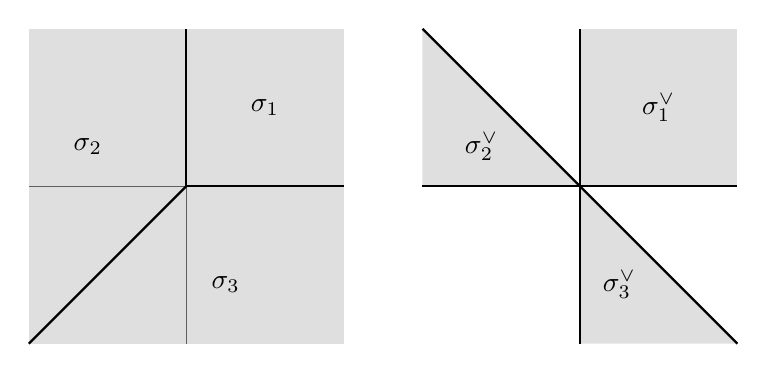
\begin{tikzpicture}
        \begin{scope}
            % Axes
            \draw (-2, 0) -- (2, 0);
            \draw (0, -2) -- (0, 2);
            % Faces
            \fill[fill=gray!50, opacity=0.5] (-2, -2) -- (2, -2) -- (2, 2) -- (-2, 2);
            % Liens
            \draw[thick] (0, 0) -- (2, 0);
            \draw[thick] (0, 0) -- (0, 2);
            \draw[thick] (0, 0) -- (-2, -2);
            % Nodes
            \node at (1, 1) {$\sigma_1$};
            \node at (-1.25, 0.5) {$\sigma_2$};
            \node at (0.5, -1.25) {$\sigma_3$};
        \end{scope}
        \begin{scope}[shift={(5, 0)}]
            % Axes
            \draw (-2, 0) -- (2, 0);
            \draw (0, -2) -- (0, 2);
            % Faces
            \fill[fill=gray!50, opacity=0.5] (0, 0) -- (2, 0) -- (2, 2) -- (0, 2);
            \fill[fill=gray!50, opacity=0.5] (0, 0) -- (-2, 0) -- (-2, 2);
            \fill[fill=gray!50, opacity=0.5] (0, 0) -- (0, -2) -- (2, -2);
            % Liens
            \draw[thick] (-2, 0) -- (2, 0);
            \draw[thick] (0, -2) -- (0, 2);
            \draw[thick] (-2, 2) -- (2, -2);
            % Nodes
            \node at (1, 1) {$\sigma_1^\vee$};
            \node at (-1.25, 0.5) {$\sigma_2^\vee$};
            \node at (0.5, -1.25) {$\sigma_3^\vee$};
        \end{scope}
    \end{tikzpicture} \]
    One computes
    \[ U_{\sigma_1} = \Spec(k[x, y]), \quad U_{\sigma_2} = \Spec(k[x^{-1}, yx^{-1}]), \quad U_{\sigma_3} = \Spec(k[y^{-1}, xy^{-1}]) , \]
    and gluing gives $X(\Delta) \isom \PP_k^2$.

    Conversely, given a toric variety $X$ with torus $T$, one construct a fan $\Delta \subset N_\RR$ with $N = \Hom(\GG_m, T)$ the lattice of one-parameter subgroups and $M = \Hom(T, \GG_m)$ the character lattice of $T$. For any one-parameter subgroup $\lambda : \GG_m \to T$, denote by $\lim_{t \to 0} \lambda(t)$ the limit point in $X$ if it exists. Partitioning $N_\RR$ based on the limit points yields a fan $\Delta$ (after taking closures), such that the corresponding toric variety $X(\Delta)$ is isomorphic to $X$.

    In the example of $X = \PP^2_k$ with maximal torus $T = \GG_m^2$, the one-parameter subgroups of $T$ are given by $\lambda^{a, b}(t) = (t^a, t^b)$ for $a, b \in \ZZ$. The limit points are
    \[ \lim_{t \to 0} \lambda^{a, b}(t) = \left\{ \begin{array}{cl}
        (0 : 0 : 1) & \textup{ if } a, b > 0, \\
        (1 : 0 : 0) & \textup{ if } a < 0 \textup{ and } a < b, \\
        (0 : 1 : 0) & \textup{ if } b < 0 \textup{ and } a > b, \\
        (1 : 0 : 1) & \textup{ if } a = 0 \textup{ and } b > 0, \\
        (0 : 1 : 1) & \textup{ if } b = 0 \textup{ and } a > 0, \\
        (1 : 1 : 0) & \textup{ if } a = b < 0, \\
        (1 : 1 : 1) & \textup{ if } a = 0 = 0.
    \end{array} \right. \]
    Indeed, this corresponds to the fan as given above.
\end{example}

\begin{example}{toric-variety}
    Projective space $\PP^n$ is a toric variety, since the torus
    \[ T = \{ (1 : t_1 : t_2 : \cdots : t_n) : t_i \ne 0 \} \subset \PP^n \]
    is open and dense, and the action of $T$ on itself extends to $\PP^n$ via
    \[ T \times \PP^n \to \PP^n, \quad \left( (t_1, \ldots, t_n), (x_0 : x_1 : \cdots x_n) \right) \mapsto (x_0 : t_1 x_1 : \cdots t_n x_n) . \]
\end{example}

\begin{topic}{formal-completion}{formal completion}
    Let $X$ be a \tref{noetherian-scheme}{noetherian} \tref{scheme}{scheme}, and $Y \subset X$ a \tref{closed-immersion}{closed subscheme}, defined by a \tref{sheaf-of-ideals}{sheaf of ideals} $\mathcal{I}$. The \textbf{formal completion} of $X$ along $Y$, denoted $(\hat{X}, \mathcal{O}_{\hat{X}})$, is the \tref{ringed-space}{locally ringed space} whose topological space $\hat{X}$ is the topological space of $Y$, and $\mathcal{O}_{\hat{X}}$ is the \tref{CT:inverse-limit}{inverse limit} $\varprojlim_n \mathcal{O}_X / \mathcal{I}^n$.
    
    When $X = \Spec R$ is an \tref{affine-scheme}{affine scheme} and $I \subset R$ an ideal, the formal completion is also known as the \textbf{formal spectrum} of $R$ along $I$, denoted $\textup{Spf}(R)$.
\end{topic}

\begin{example}{formal-completion}
    Let $k$ be a field and consider $X = \Spec k[x]$ with closed subscheme $Y \subset X$ given by the ideal $(x)$. Then the formal completion $\hat{X}$ has a topological space consisting of one point, with sheaf of rings given by $\mathcal{O}_{\hat{X}}(\hat{X}) = k \llbracket x \rrbracket$.
    
    Note that the locally ringed space $\hat{X}$ is not the same as $\Spec k \llbracket x \rrbracket$, whose topological space has two points, given by the prime ideals $(0)$ and $(x)$.
\end{example}

\begin{topic}{noetherian-formal-scheme}{noetherian formal scheme}
    A \textbf{noetherian formal scheme} is a \tref{ringed-space}{locally ringed space} $(\mathfrak{X}, \mathcal{O}_\mathfrak{X})$, which has a finite open cover $\{ \mathfrak{U}_i \}$ such that for each $i$, the pair $(\mathfrak{U}_i, \mathcal{O}_\mathfrak{X}|_{\mathfrak{U}_i})$ is isomorphic to the \tref{formal-completion}{formal completion} of some \tref{noetherian-scheme}{noetherian scheme} $X$ along a closed subscheme $Y \subset X$.
\end{topic}

\begin{topic}{algebraic-space}{algebraic space}
    Let $S$ be a \tref{scheme}{scheme} in $\textbf{Sch}_\textup{fppf}$. An \textbf{algebraic space} over $S$ is a \tref{CT:presheaf}{presheaf}
    \[ F : (\textbf{Sch}/S)_\textup{fppf}^\textup{op} \to \textbf{Set} \]
    such that
    \begin{itemize}
        \item $F$ is a \tref{CT:sheaf}{sheaf},
        \item the diagonal $\Delta : F \to F \times F$ is \textit{representable}, that is, for every $T \in (\textbf{Sch}/S)_\textup{fppf}$ and $\xi \in (F \times F)(T) = F(T) \times F(T)$ the fiber product $T \times_{(F \times F)} F$ is representable by a scheme,
        \item there exists a scheme $X \in (\textbf{Sch}/S)_\textup{fppf}$ and a representable map $X \to F$ which is surjective and étale. That is, for every $T \in (\textbf{Sch}/S)_\textup{fppf}$ and $\xi \in F(T)$ the map $X \times_F T \to T$ (of schemes) is surjective and \tref{AG:etale-morphism}{étale}.
    \end{itemize}
\end{topic}

\begin{topic}{mordell-weil-theorem}{Mordell--Weil theorem}
    The \textbf{Mordell--Weil theorem} states that for an \tref{abelian-variety}{abelian variety} $A$ and a \tref{NT:number-field}{number field} $K$, the $K$-rational points $A(K)$ form a \tref{GT:finitely-generated-group}{finitely generated} \tref{GT:abelian-group}{abelian} \tref{GT:group}{group}, called the \textbf{Mordell--Weil group}.
\end{topic}

\begin{topic}{ample-invertible-sheaf}{(very) ample invertible sheaf}
    Let $X$ be a \tref{scheme}{scheme} over $S$. An \tref{invertible-sheaf}{invertible sheaf} $\mathcal{L}$ on $X$ is called \textbf{very ample} relative to $S$, if there is an \tref{immersion}{immersion} $i : X \to \PP_S^n$ for some $n$, such that $\mathcal{L} \isom i^*(\mathcal{O}_{\PP_S^n}(1))$.
    
    An invertible sheaf $\mathcal{L}$ on a \tref{noetherian-scheme}{noetherian scheme} $X$ is \textbf{ample} if for every \tref{coherent-sheaf}{coherent sheaf} $\mathcal{F}$ on $X$, there is an integer $n_0 > 0$ such that for every $n \ge n_0$ the sheaf $\mathcal{F} \otimes \mathcal{L}^{\otimes n}$ is generated by its global sections.
\end{topic}

\begin{example}{ample-invertible-sheaf}
    When $X = \Spec R$ is affine, any invertible sheaf is ample, because every (quasi-)coherent sheaf on an affine scheme is generated by its global sections.
\end{example}

\begin{topic}{cech-cohomology}{Čech cohomology}
    Let $X$ be a \tref{TO:topological-space}{topological space}, $\mathcal{U} = \{ U_i \}_{i \in I}$ an open covering of $X$, and $\mathcal{F}$ a \tref{AG:sheaf}{sheaf} on $X$. Put a well-ordering on $I$ and for convenience write $U_{i_0 \cdots i_p}$ for $U_{i_0} \cap \cdots \cap U_{i_p}$.
    
    The \textbf{Čech complex} of $\mathcal{F}$ with respect to $\mathcal{U}$ is the complex
    \[ C^p(\mathcal{U}, \mathcal{F}) = \prod_{i_0 < \cdots < i_p} \mathcal{F}(U_{i_0 \cdots i_p}) \qquad p \ge 0 , \]
    with differential
    \[ d^p : C^p(\mathcal{U}, \mathcal{F}) \to C^{p + 1}(\mathcal{U}, \mathcal{F}) \]
    \[ (d^p \alpha)_{i_0 , \ldots , i_{p + 1}} = \sum_{k = 0}^{p + 1} (-1)^k \alpha_{i_0 , \ldots , \hat{i}_k, \ldots, i_{p + 1}} | _{U_{i_0 \cdots i_{p + 1}}} . \]
    For all $p \ge 0$ the $p$-th \textbf{Čech cohomology group} of $\mathcal{F}$ with respect to $\mathcal{U}$ is the cohomology group
    \[ \hat{H}^p(\mathcal{U}, \mathcal{F}) = H^p(C^\bdot(\mathcal{U}, \mathcal{F})) . \]
\end{topic}

\begin{example}{cech-cohomology}
    Note that 
    \[ d^0 : C^0(\mathcal{U}, \mathcal{F}) = \prod_{i \in I} \mathcal{F}(U_i) \to C^1(\mathcal{U}, \mathcal{F}) = \prod_{i < j} \mathcal{F}(U_{ij}) \]
    sends $s = (s_i)_{i \in I}$ to $d^0 s = \left(s_j|_{U_i} - s_i|_{U_j}\right)_{ij}$. Therefore, by the sheaf property $\hat{H}^0(\mathcal{U}, \mathcal{F}) = \ker d^0 \isom \mathcal{F}(X)$.
    % H^1 isomorphic to line bundles that trivialize on each U_i
\end{example}

\begin{topic}{sheaf-differentials}{sheaf of differentials}
    Let $f : X \to Y$ be a morphism of \tref{scheme}{schemes}. Covering $X$ and $Y$ by affine opens $V = \Spec A \subset Y$ and $U = \Spec B \subset X$ such that $f(U) \subset V$, consider the sheaf $\widetilde{\Omega_{B/A}}$ on $U$, the sheaf \tref{sheaf-associated-to-module}{associated} to the module \tref{AA:derivation}{$\Omega_{B/A}$}. Gluing these sheaves together gives $\Omega_{X/Y}$, the \textbf{relative sheaf of differentials}.
    
    Alternatively, consider the diagonal morphism $\Delta_{X/Y} : X \to X \times_Y X$, and view $X \xrightarrow{\sim{}} \Delta(X)$ as a \tref{closed-immersion}{closed subscheme} of an open subset $W$ of $X \times_Y X$, with corresponding sheaf of ideals $\mathcal{I}$. Then
    \[ \Omega_{X/Y} = \Delta_{X/Y}^*(\mathcal{I}/\mathcal{I}^2) . \]
\end{topic}

\begin{example}{sheaf-differentials}
    Let $f : X \to Y$ be locally of finite type. If $f$ is \tref{unramified-morphism}{unramified} then $\Omega_{X/Y} = 0$. Namely, since $\Omega_{X/Y}$ behaves well with respect to base change, this can be checked locally, that is, we can assume $Y = \Spec B$ and $X = \Spec A$ with $A \to B$ a local homomorphism of local rings. Using \tref{AA:nakayamas-lemma}{Nakayama's lemma} this reduces to the case where $A$ and $B$ are fields. Being unramified means that $A \subset B$ is a \tref{AA:separable-field-extension}{separable field extension}, and then it is clear that $\Omega_{B/A} = 0$.
    
    Conversely, if $\Omega_{X/Y} = 0$ then $f$ is unramified.
\end{example}

\begin{topic}{albanese-variety}{Albanese variety}
    Let $X$ be a connected \tref{complete-variety}{complete} \tref{variety}{variety} over an algebraically closed field $k$, with a basepoint. Then there exists an \tref{abelian-variety}{abelian variety} $\textup{Alb}(X)$, the \textbf{Albanese variety} of $X$, and a morphism of pointed varieties $i : X \to \textup{Alb}(X)$, the \textbf{Albanese map}, with the universal property that for any other abelian variety $A$ and morphism of pointed varieties $f : X \to A$, there exists a unique morphism of abelian varieties $f' : \textup{Alb}(X) \to A$ such that $f = f' \circ i$.
    \[ \begin{tikzcd} X \arrow{r}{i} \arrow[swap]{dr}{f} &  \textup{Alb}(X) \arrow[dashed]{d}{f'} \\ &  A \end{tikzcd} \]
\end{topic}

\begin{topic}{torsion-sheaf}{torsion sheaf}
    A \textbf{torsion sheaf} is a \tref{sheaf}{sheaf} $\mathcal{F}$ such that $\mathcal{F}(U)$ is a \tref{GT:torsion-group}{torsion} \tref{GT:abelian-group}{abelian group} for every $U$.
\end{topic}

\begin{topic}{flag-variety}{flag variety}
    A \textbf{flag} in a finite-dimensional \tref{LA:vector-space}{vector space} $V$ over a field $k$ is a strictly increasing sequence of subspaces
    \[ 0 = V_0 \subsetneq V_1 \subsetneq \cdots \subsetneq V_m = V . \]
    A flag is \textbf{complete} if $m = \dim V$ and $\dim_k V_i = i$ for all $i$, otherwise it is \textbf{partial}. The \textit{signature} of the flag is the sequence $(d_1, \ldots, d_m)$ where $d_i = \dim_k V_i$.
    
    Given a signature, the set of all flags with such signature is called the \textbf{flag variety} of that signature. It naturally has the structure of a \tref{projective-morphism}{projective} \tref{variety}{variety}.
\end{topic}

\begin{example}{flag-variety}
    The \textit{complete flag variety} (corresponding to signature $(1, \ldots, n)$) is $\textup{GL}_n(k) / B_n(k)$. Namely, all flags are conjugate via base change, and the stabilizer of any given flag is isomorphic to $B_n(k)$, the group of invertible upper triangular matrices.
\end{example}

\begin{example}{flag-variety}
    When $m = 2$, the flag variety parametrizes linear subspaces of $V$. That is, the flag variety is isomorphic to the \tref{LA:grassmannian}{Grassmannian} $\textup{Gr}(d_1, V)$.
\end{example}

\begin{topic}{regular-morphism}{regular morphism}
    Let $f : X \to Y$ be a morphism of \tref{scheme}{schemes}, and assume that all fibers $X_y$ are \tref{noetherian-scheme}{locally noetherian}. Then $f$ is \textbf{regular} at $x \in X$ if $f$ is \tref{flat-morphism}{flat} at $x$ and the fiber $X_{f(x)}$ is \tref{geometrically-regular}{geometrically regular} at $x$ over $k(y)$. The morphism $f$ is \textbf{regular} if it is regular at all points $x \in X$.
\end{topic}

\begin{example}{regular-morphism}
    Every \tref{smooth-morphism}{smooth morphism} is regular, but not conversely. Namely, for any field $k$, the morphism $\Spec k \llbracket t \rrbracket \to \Spec k$ is regular but not smooth, since $k \llbracket t \rrbracket$ is not finitely presented as $k$-algebra. 
\end{example}

\begin{topic}{local-to-global-sequence}{local-to-global Ext sequence}
    Let $X$ be a \tref{scheme}{scheme} and $\mathcal{F}$ and $\mathcal{G}$ \tref{O-module}{$\mathcal{O}_X$-modules}. Then there is a \tref{HA:spectral-sequence}{spectral sequence} (a special case of the \tref{HA:grothendieck-spectral-sequence}{Grothendieck spectral sequence})
    \[ E_2^{p, q} = H^p(X, \mathcal{E}\textup{xt}_X^q(\mathcal{F}, \mathcal{G})) \Rightarrow \textup{Ext}_X^{p + q}(\mathcal{F}, \mathcal{G}) . \]
    In particular, this gives the \textbf{local-to-global Ext sequence}
    \[ 0 \to H^1(X, \mathcal{H}\textup{om}(\mathcal{F}, \mathcal{G})) \to \textup{Ext}_X^1(\mathcal{F}, \mathcal{G}) \to H^0(X, \mathcal{E}\textup{xt}_X^1(\mathcal{F}, \mathcal{G})) \to H^2(X, \mathcal{H}\textup{om}(\mathcal{F}, \mathcal{G})) \to \textup{Ext}_X^2(\mathcal{F}, \mathcal{G}) \]
\end{topic}

\begin{topic}{vector-bundle}{vector bundle}
    A \textbf{vector bundle} is a \tref{free-sheaf}{locally free sheaf} $\mathcal{E}$ of finite rank.
\end{topic}

\begin{topic}{slope-vector-bundle}{slope vector bundle}
    The \textbf{slope} of a \tref{vector-bundle}{vector bundle} $\mathcal{E}$ over a \tref{algebraic-curve}{curve} $C$ is the number $\mu(\mathcal{E}) = \deg \mathcal{E} / \textup{rk} \mathcal{E}$.
\end{topic}

\begin{example}{slope-vector-bundle}
    For any semistable (resp. stable) vector bundle $\mathcal{E}$ and quotient $\mathcal{E} \twoheadrightarrow \mathcal{G}$ we have $\mu(\mathcal{E}) \le \mu(\mathcal{G})$ (resp. $\mu(\mathcal{E}) < \mathcal{G}$). Namely, given an exact sequence $0 \to \mathcal{F} \to \mathcal{E} \to \mathcal{G} \to 0$ we have
    \[ \begin{aligned} \mu(\mathcal{F}) \genfrac{\{}{\}}{0pt}{1}{\le}{<} \mu(\mathcal{E}) &\implies \deg \mathcal{F} \cdot \textup{rk } \mathcal{E} \genfrac{\{}{\}}{0pt}{1}{\le}{<} \deg \mathcal{E} \cdot \textup{rk } \mathcal{F} \\ &\implies \deg \mathcal{G} \cdot \textup{rk } \mathcal{E} \genfrac{\{}{\}}{0pt}{1}{\ge}{>} \deg \mathcal{E} \cdot \textup{rk } \mathcal{G} \implies \mu(\mathcal{G}) \genfrac{\{}{\}}{0pt}{1}{\ge}{>} \mu(\mathcal{E})  , \end{aligned} \]
    since $\deg \mathcal{F} = \deg \mathcal{E} - \deg \mathcal{G}$ and $\textup{rk } \mathcal{F} = \textup{rk } \mathcal{E} - \textup{rk } \mathcal{G}$.
\end{example}

\begin{topic}{stable-vector-bundle}{(semi)stable vector bundle}
    A \tref{vector-bundle}{vector bundle} $\mathcal{E}$ over a \tref{algebraic-curve}{curve} $C$ is \textbf{semistable} (resp. \textbf{stable}) if $\mu(\mathcal{F}) \le \mu(\mathcal{E})$ (resp. $\mu(\mathcal{F}) < \mu(\mathcal{E})$) for every vector subbundle $0 \ne \mathcal{F} \subsetneq \mathcal{E}$, where $\mu(\mathcal{E})$ denotes the \tref{slope-vector-bundle}{slope} of $\mathcal{E}$.
\end{topic}

\begin{topic}{harder-narasimhan-filtration}{Harder--Narasimhan filtration}
    Let $\mathcal{E}$ be a \tref{vector-bundle}{vector bundle} over a \tref{algebraic-curve}{curve} $C$. There exists a unique filtration by subbundles
    \[ 0 = \mathcal{E}_0 \subset \mathcal{E}_1 \subset \cdots \subset \mathcal{E}_{r + 1} = \mathcal{E} \]
    such that $\mathcal{E}_{i + 1}/\mathcal{E}_i$ are \tref{stable-vector-bundle}{semistable vector bundles} with slope $\mu_i$, where $\mu_1 > \mu_2 > \cdots > \mu_r$. This filtration is called the \textbf{Harder--Narasimhan filtration}.
    
    It is constructed as follows. If $\mathcal{E}$ is not semistable, take $0 \ne \mathcal{F} \subsetneq \mathcal{E}$ with maximal \tref{slope-vector-bundle}{slope} and among those with maximal rank. Then $\mathcal{E}_1 := \mathcal{F}$ is semistable by construction, and repeat the process with $\mathcal{E}/\mathcal{F}$.
\end{topic}

\begin{topic}{nef-line-bundle}{nef line bundle}
    A \tref{invertible-sheaf}{line bundle} $\mathcal{L}$ on a \tref{scheme}{scheme} $X$, \tref{proper-morphism}{proper} over a field $k$, is \textbf{nef} (\textit{numerically effective}) if $\deg \mathcal{L}|_C \ge 0$ for every (\tref{closed-immersion}{closed} \tref{TO:irreducible-space}{irreducible}) \tref{algebraic-curve}{curve} $C$ in $X$.
\end{topic}

\begin{topic}{riemann-roch-theorem}{Riemann--Roch theorem}
    Let $C$ be a smooth projective connected \tref{algebraic-curve}{curve} over a field $k$, and $\mathcal{E}$ a \tref{vector-bundle}{vector bundle} over $C$. The \textbf{Riemann--Roch theorem} states that
    \[ \chi(\mathcal{E}) = \dim_k H^0(C, \mathcal{E}) - \dim_k H^1(C, \mathcal{E}) = (1 - g) \textup{rk } \mathcal{E} + \deg \mathcal{E} , \]
    where $g$ is the \tref{geometric-genus}{genus} of $C$ and $\chi(\mathcal{E})$ the \tref{sheaf-euler-characteristic}{Euler characteristic} of $\mathcal{E}$.
\end{topic}

\begin{topic}{algebraic-scheme}{algebraic scheme}
    An \textbf{algebraic scheme} over a field $k$ is a \tref{scheme}{scheme} $X$ over $k$ such that the structure morphism $X \to \Spec k$ is \tref{finite-type}{of finite type}.
\end{topic}

\begin{topic}{projective-variety}{(quasi-)projective variety}
    A \tref{variety}{variety} over a field $k$ is \textbf{projective} if it is isomorphic to a \tref{closed-immersion}{closed} subvariety of some projective space $\PP^n_k$.
    
    A \tref{variety}{variety} over a field $k$ is \textbf{quasi-projective} if it is isomorphic to an open subvariety of a projective variety.
\end{topic}

\begin{topic}{affine-variety}{(quasi-)affine variety}
    A \tref{variety}{variety} over a field $k$ is \textbf{affine} if it is isomorphic to a \tref{closed-immersion}{closed} subvariety of some affine space $\AA^n_k$.
    
    A \tref{variety}{variety} over a field $k$ is \textbf{quasi-affine} if it is isomorphic to an open subvariety of an affine variety.
\end{topic}

\begin{example}{affine-variety}
    The variety $\AA^2 \setminus \{ (0, 0) \}$ is quasi-affine, but not affine.
\end{example}

\begin{topic}{hodge-deligne-polynomial}{Hodge--Deligne polynomial}
    Let $X$ be a \tref{variety}{variety} over $\CC$. The \tref{AT:cohomology-compact-support}{cohomology groups with compact support} $H_c^k(X, \CC)$ naturally carry a \tref{LA:mixed-hodge-structure}{mixed Hodge structure}. The \textbf{Hodge--Deligne polynomial} of $X$ is the polynomial
    \[ \mu(X) = \sum_{k, p, q} h_c^{k; p, q}(X) u^p v^q t^k \in \ZZ[u, v, t] , \]
    where $h_c^{k; p, q}(X) = \dim_\CC \textup{Gr}_F^p \textup{Gr}^W_{p + q} H_c^k(X, \CC)$ are the mixed Hodge numbers.
\end{topic}

\begin{topic}{e-polynomial}{E-polynomial}
    Let $X$ be a \tref{variety}{variety} over $\CC$. The \tref{AT:cohomology-compact-support}{cohomology groups with compact support} $H_c^k(X, \CC)$ naturally carry a \tref{LA:mixed-hodge-structure}{mixed Hodge structure}. The \textbf{$E$-polynomial} of $X$ is the polynomial
    \[ e(X) = \sum_{k, p, q} (-1)^k h_c^{k; p, q}(X) u^p v^q \in \ZZ[u, v] , \]
    where $h_c^{k; p, q}(X) = \dim_\CC \textup{Gr}_F^p \textup{Gr}^W_{p + q} H_c^k(X, \CC)$ are the mixed Hodge numbers.
\end{topic}

\begin{example}{e-polynomial}
    For a closed subvariety $Z \subset X$ with complement $U = X \setminus Z$, there is a long exact sequence of mixed Hodge structures
    \[ \cdots \to H_c^i(U, \CC) \to H_c^i(X, \CC) \to H_c^i(Z, \CC) \to H_c^{i + 1}(U, \CC) \to \cdots \]
    which shows that
    \[ e(X) = e(Z) + e(U) . \]
    Moreover, it can be shown that $e(X \times_\CC Y) = e(X) e(Y)$. This shows that $e : \textbf{Var}_\CC \to \ZZ[u, v]$ factors through the \tref{grothendieck-ring-of-varieties}{Grothendieck ring of varieties}.
\end{example}

\begin{topic}{grothendieck-ring-of-varieties}{Grothendieck ring of varieties}
    Let $S$ be a \tref{variety}{variety} over a field $k$. The \textbf{Grothendieck ring of varieties} over $S$, denoted $\textup{K}_0(\textbf{Var}_S)$, is defined as the quotient of the \tref{GT:free-group}{free abelian group} on the isomorphism classes of varieties over $S$, by relations of the form
    \[ [X] = [Z] + [U] , \]
    where $Z \subset X$ is a closed subvariety and $U = X \setminus Z$ its open complement. Multiplication is defined by
    \[ [X] \cdot [Y] = [(X \times_S Y)_\textup{red}] \]
    and extended linearly.
\end{topic}

\begin{example}{grothendieck-ring-of-varieties}
    \begin{itemize}
        \item Denote by $\mathbb{L}$ the class of the affine line $\AA^1_k$. Then $[\AA^n_k] = \mathbb{L}^n$.
        \item From the relation $\PP^n_k \setminus \PP^{n - 1}_k \cong \AA^n_k$ one shows inductively that $[\PP^n_k] = \mathbb{L}^n + \cdots + \mathbb{L} + 1$ for all $n > 0$.
        \item Consider the variety $\textup{SL}_2 = \Spec k[a, b, c, d] / (ad - bc - 1)$. Then
        \[ \def\arraystretch{1.5}
        \begin{array}{ccccc}
            [\textup{SL}_2] & = & [\{ (a, b, c, d) \in \AA^4_k \mid a = 0, \; bc = -1 \}] & + & [\{ (a, b, c, d) \in \AA^4_k \mid a \ne 0, \; d = (1 + bc) / a \}] \\
                & = & \mathbb{L} (\mathbb{L} - 1) & + & \mathbb{L}^2 (\mathbb{L} - 1) \\
                & = & \mathbb{L}^3 - \mathbb{L} . &
        \end{array} \]
    \end{itemize}
    
\end{example}

\begin{topic}{excellent-scheme}{(quasi-)excellent scheme}
    A \tref{scheme}{scheme} $X$ is \textbf{(quasi-)excellent} if it has an affine open cover by schemes $\Spec R_i$ with $R_i$ an \tref{AA:excellent-ring}{(quasi-)excellent} ring.
\end{topic}

\begin{topic}{genus-degree-formula}{genus-degree formula}
    Let $C \subset \PP^2$ be a \tref{smooth-morphism}{smooth} \tref{projective-variety}{projective} \tref{algebraic-curve}{curve} given by a homogeneous polynomial of degree $d$. The \textbf{genus-degree formula} expresses the \tref{geometric-genus}{genus} $g$ of $C$ in terms of $d$,
    \[ g = \frac{1}{2}(d - 1)(d - 2) . \]
\end{topic}

\begin{example}{genus-degree-formula}
    Let $E \subset \PP^2$ be given by $Y^2Z - X^3 + XZ^2 = 0$ (of degree $3$), then the genus of $E$ is $\frac{1}{2}(d - 1)(d - 2) = 1$.
\end{example}

\begin{topic}{elliptic-curve}{elliptic curve}
    An \textbf{elliptic curve} is a \tref{smooth-morphism}{smooth} \tref{projective-variety}{projective} \tref{algebraic-curve}{algebraic curve} $E$ over a field $k$ of \tref{geometric-genus}{genus} one, together with a specified point $O$ on $E$. An elliptic curve comes naturally with a group structure, making it an \tref{abelian-variety}{abelian variety}, where $O$ is the unit of the group structure.
\end{topic}

\begin{topic}{fano-variety}{Fano variety}
    A \textbf{Fano variety} is a \tref{complete-variety}{complete variety} whose anti-\tref{canonical-sheaf}{canonical sheaf} $\omega_X^\vee$ is \tref{ample-invertible-sheaf}{ample}.
\end{topic}

\begin{topic}{del-pezzo-surface}{del Pezzo surface}
    A \textbf{del Pezzo surface} is a two-dimensional \tref{fano-variety}{Fano variety}.
\end{topic}

\begin{topic}{kodaira-dimension}{Kodaira dimension}
    Let $X$ be a \tref{projective-variety}{projective variety} over a field $k$. The \textbf{Kodaira dimension} $\kappa(X)$ of $X$ is the \tref{AA:transcendence-degree}{transcendence degree} over $k$ of the ring
    \[ \bigoplus_{n \ge 0} H^0(X, \omega_X^{\otimes n}) \]
    minus $1$, where $\omega_X$ is the \tref{canonical-sheaf}{canonical sheaf} of $X$.
\end{topic}

\begin{topic}{rational-curve}{rational curve}
    A \textbf{rational curve} is an \tref{algebraic-curve}{algebraic curve} which is \tref{birational-map}{birationally equivalent} to the projective line.
\end{topic}

\begin{topic}{zariski-main-theorem}{Zariski's main theorem}
    \textbf{Zariski's main theorem} states that any \tref{separated-morphism}{separated} \tref{quasi-finite-morphism}{quasi-finite} morphism $f : Y \to X$ with $X$ \tref{quasi-compact-scheme}{quasi-compact}, factors as $f' \circ g$, where $f' : Y \to Y'$ is an \tref{open-immersion}{open immersion} and $g : Y' \to X$ is a \tref{finite-morphism}{finite morphism}.
\end{topic}

\begin{topic}{brauer-group}{Brauer group}
    Let $X$ be a \tref{scheme}{scheme}. The \textbf{Brauer group} of $X$ is the second étale cohomology group
    \[ \textup{Br}(X) = H^2_\textup{ét}(X, \GG_m) . \]
\end{topic}

\begin{topic}{rationally-connected-variety}{rationally connected variety}
    A \textbf{rationally connected variety} is a \tref{projective-variety}{projective variety} $X$ over an \tref{AA:algebraically-closed-field}{algebraically closed field} $k$ such that through every two points passes the image of a morphism $\gamma : \PP^1_k \to X$.
\end{topic}

\begin{topic}{quasi-affine-scheme}{quasi-affine scheme}
    A \tref{scheme}{scheme} is \textbf{quasi-affine} if it is \tref{quasi-compact-scheme}{quasi-compact} and isomorphic to an open subscheme of an \tref{affine-scheme}{affine scheme}.
\end{topic}

\begin{topic}{hasse-weil-zeta-function}{Hasse--Weil zeta function}
    Let $X$ be a \tref{variety}{variety} over a finite field $\FF_q$. The \textbf{Hasse--Weil zeta function} of $X$ is given by
    \[ Z(X, t) = \exp \left( \sum_{n = 1}^{\infty} |X(\FF_{q^n})| \frac{t^n}{n} \right) \in \QQ \llbracket t \rrbracket . \]
\end{topic}

\begin{example}{hasse-weil-zeta-function}
    For $X = \PP^m$, we have $|X(\FF_{q^n})| = \sum_{j = 0}^{m} q^{jn}$ for all $n$, so
    \[ Z(\PP^m, t) = \exp \left( \sum_{n = 1}^{\infty} \sum_{j = 0}^{m} \frac{q^{jn} t^n}{n} \right) = \prod_{j = 0}^{m} \frac{1}{(1 - q^j t)} . \]
    In particular,
    \[ Z(\star, t) = \frac{1}{1 - t} \quad \textup{ and } \quad Z(\PP^1, t) = \frac{1}{(1 - t)(1 - qt)} . \]
\end{example}

\begin{example}{hasse-weil-zeta-function}
    The Hasse--Weil zeta function has many different expressions. For $r \ge 1$, let $a_r$ be the number of closed points of $X$ of degree $r$. Then,
    \[ \begin{aligned}
        Z(X, t)
            &= \exp \left( \sum_{n \ge 1} \frac{|X(\FF_{q^n})|}{n} t^n \right) \\
            &= \exp \left( \sum_{n \ge 1} \sum_{r | n} \frac{r \cdot a_r}{n} t^n \right) \\
            &= \exp \left( \sum_{r \ge 1} a_r \sum_{\ell \ge 1} \frac{t^{\ell r}}{\ell} \right) \\
            &= \exp \left( \sum_{r \ge 1} - a_r \log (1 - t^r) \right) \\
            &= \prod_{r \ge 1} (1 - t^r)^{-a_r} \\
            &= \prod_{x \in X_{\textup{cl}}} (1 + t^{\deg(x)} + t^{2 \deg(x)} + \cdots) \\
            &= \sum_{\alpha} t^{\deg(\alpha)} ,
    \end{aligned}\]
    where $\alpha$ runs over the set of effective $0$-cycles on $X$.
\end{example}

\begin{topic}{kapranov-zeta-function}{Kapranov zeta function}
    Let $X$ be a \tref{projective-variety}{quasi-projective variety} over a field $k$. The \textbf{Kapranov zeta function} of $X$ is given by
    \[ Z(X, t) = \sum_{n \ge 0} [\textup{Sym}^n X] t^n \in 1 + t \cdot \textup{K}_0(\textbf{Var}_k) \llbracket t \rrbracket , \]
    where $\textup{Sym}^n X$ denotes the symmetric product of $X$, that is, the \tref{affine-git-quotient}{GIT quotient} $X^n \sslash S_n$, and $\textup{K}_0(\textbf{Var}/k)$ denotes the \tref{grothendieck-ring-of-varieties}{Grothendieck ring of varieties}.
    
    For any ring morphism $\mu : \textup{K}_0(\textbf{Var}_k) \to R$, the \textbf{motivic zeta function} of $X$ is given by
    \[ Z(X, t) = \sum_{n \ge 0} \mu([\textup{Sym}^n X]) t^n \in 1 + t \cdot R \llbracket t \rrbracket . \]
\end{topic}

\begin{example}{kapranov-zeta-function}
    For any closed subvariety $Y \subset X$ with complement $U$, we can identify
    \[ \begin{aligned}
        [\textup{Sym}^n X]
            &= [X^n \sslash S_n] \\
            &= \sum_{i + j = n} [S_n \cdot (Y^i \times U^j) \sslash S_n] \\
            &= \sum_{i + j = n} [Y^i \sslash S_i \times U^j \sslash S_j] \\
            &= \sum_{i + j = n} [ \textup{Sym}^i Y] \cdot [ \textup{Sym}^j U ] ,
    \end{aligned} \]
    and hence
    \[ Z(X, t) = \sum_{n \ge 0} [\textup{Sym}^n X] t^n = \sum_{\substack{n \ge 0 \\ i + j = n}} [\textup{Sym}^i Y] \cdot [\textup{Sym}^j U] t^n = Z(Y, t) \cdot Z(U, t) . \]
    This relation allows to extend the definition of $Z(X, t)$ to all varieties $X$, and, moreover, it gives a group morphism
    \[ Z(-, t) : \textup{K}_0(\textbf{Var}_k) \to 1 + t \cdot \textup{K}_0(\textbf{Var}_k) \llbracket t \rrbracket , \]
    with the multiplicative group structure on the right.
\end{example}

\begin{example}{kapranov-zeta-function}
    For $k = \FF_q$ and $\mu : X \mapsto X(\FF_q)$ the point-counting function, the motivic zeta function reduces to the \tref{hasse-weil-zeta-function}{Hasse--Weil zeta function}. Namely, the $\FF_q$-points of $\textup{Sym}^n X$ can be identified with $0$-cycles of degree $n$ on $X$, and the Hasse--Weil zeta function can be expressed as
    \[ Z(X, t) = \sum_{\alpha} t^{\deg(\alpha)} , \]
    where $\alpha$ runs over the set of effective $0$-cycles on $X$.
\end{example}

\begin{example}{kapranov-zeta-function}
    Let $\mathbb{L} = [\AA^1] \in \textup{K}_0(\textbf{Var}_k)$ be the class of the affine line. By the \tref{AA:symmetric-polynomial}{fundamental theorem of symmetric polynomials}, we have $\operatorname{Sym}^n(\AA^1) \isom \AA^n$ for all $n \ge 0$. More generally, one can show
    \[ Z(\AA^i, t) = 1 + \mathbb{L}^i t + \mathbb{L}^{2i} t^2 + \cdots = \frac{1}{1 - \mathbb{L}^i t} . \]
    In particular,
    \[ Z(\PP^n, t) = Z\left(\bigsqcup_{i = 0}^{n} \AA^i , t\right) = \prod_{i = 0}^{n} Z(\AA^i, t) = \prod_{i = 0}^{n} \frac{1}{1 - \mathbb{L}^i t} . \]
\end{example}

\begin{topic}{luna-slice-theorem}{Luna slice theorem}
    Let $G$ be a \tref{reductive-algebraic-group}{reductive} \tref{algebraic-group}{algebraic group}, acting on an \tref{affine-variety}{affine variety} $X$, over an \tref{AA:algebraically-closed-field}{algebraically closed field} $k$ of characteristic zero. Let $x \in X(k)$ be a smooth point, with \tref{GT:stabilizer}{stabilizer} $G_x$, whose \tref{GT:orbit}{orbit} $O_x$ is closed. Then \textbf{Luna's slice theorem} states that there exists a smooth affine subvariety $Y \subset X$ containing $x$, invariant under $G_x$, such that
    \begin{enumerate}[(i)]
        \item the \tref{tangent-sheaf}{tangent space} at $x$ decomposes as $\mathcal{T}_{X, x} = \mathcal{T}_{Y, x} \oplus \mathcal{T}_{O_x, x}$,
        \item the $G$-equivariant map
        \[ \psi : G \times_{G_x} Y \to X, \quad (g, y) \mapsto g \cdot y , \]
        is \tref{etale-morphism}{étale}, and its image $U$ is open in $X$,
        \item the map
        \[ Y/G_x \isom (G \times_{G_x} Y) / G \xrightarrow{\psi / G} U / G \]
        is étale at $[x]$,
        \item the maps $\psi$ and $G \times_{G_x} Y \to (G \times_{G_x} Y) / G \to Y / G_x$ induce an isomorphism
        \[ G \times_{G_x} Y \isom U \times_{U/G} (Y/G_x) . \]
    \end{enumerate}
    The subvariety $Y$ is called an \textit{étale slice} at $x$.
\end{topic}

\begin{topic}{weighted-projective-space}{weighted projective space}
    Let $k$ be a \tref{AA:ring}{commutative ring}. A \textbf{weighted projective space} over $k$ is the \tref{projective-variety}{projective variety}
    \[ \PP_k(a_0, \ldots, a_n) = \textup{Proj}(k[x_0, \ldots, x_n]) , \]
    with $\deg(x_i) = a_i$, for integers $a_i \in \ZZ$.
\end{topic}

\begin{topic}{moduli-space}{moduli space}
    Let $F : \textbf{Sch}^\textup{op} \to \textbf{Set}$ be a \tref{CT:functor}{functor}.
    A scheme $M$ is a \textbf{fine moduli space} for $F$ if $M$ \tref{CT:representable-functor}{represents} $F$, that is, there is a \tref{CT:natural-transformation}{natural} isomorphism
    \[ F \isom \Hom_\textbf{Sch}(-, M) . \]
    A scheme $M$ is a \textbf{coarse moduli space} for $F$ if there exists a natural transformation
    \[ F \Rightarrow \Hom_\textbf{Sch}(-, M) , \]
    which is universal among all such natural transformations.
\end{topic}

\begin{topic}{valuative-criterion}{valuative criterion}
    Let $f : X \to Y$ be a morphism of \tref{scheme}{schemes} over a scheme $S$, and assume $f$ is \tref{finite-type}{of finite type} and \tref{separated-morphism}{quasi-separated}. The \textbf{valuative criterion} states that $f$ is \tref{proper-morphism}{proper} if and only if for every diagram
    \[ \begin{tikzcd}
        \Spec K \arrow{r} \arrow{d} & X \arrow{d}{f} \\ \Spec R \arrow[dashed]{ur} \arrow{r} & Y
    \end{tikzcd} \]
    where $R$ is a \tref{AA:valuation-ring}{valuation ring} and $K$ its \tref{AA:field-of-fractions}{field of fractions}, there exists a unique morphism $\Spec R \to X$ making the diagram commute. If $Y$ is \tref{noetherian-scheme}{locally noetherian}, it suffices to check the criterion for \tref{AA:discrete-valuation-ring}{discrete valuation rings} $R$.
    
    More precisely, the existence of the dashed arrow corresponds to $f$ being \tref{TO:universally-closed}{universally closed}, and the uniqueness corresponds to $f$ being \tref{separated-morphism}{separated}.
\end{topic}

\begin{example}{valuative-criterion}
    The valuative criterion for properness can be used to show that the morphism $f : \AA^1_k \to \Spec k$ is not proper. Namely, take $R = k[t]_{(t)}$ with $K = k(t)$. Considering the diagram with $\AA^1_k \to \Spec K$ given by $k[x] \to k(t)$, $x \mapsto 1/t$, there does not exist a map $k[x] \to k[t]_{(t)}$ completing the diagram.
\end{example}

\begin{example}{valuative-criterion}
    The valuative criterion for properness can be used to show that the morphism $f : \PP^n \to \Spec \ZZ$ is proper. It can be assumed that $R$ is a discrete valuation ring. A morphism $\Spec K \to \PP^n$ can be expressed in terms of homogeneous coordinates $(a_0 : a_1 : \ldots : a_n)$, with $a_i \in K$ not all zero. Let $a_\textup{min} = \min \{ a_i : 1 \le i \le n, a_i \ne 0 \}$ with respect to the valuation of $R$. Then the $R$-point of $\PP^n$ we are looking for is given by
    \[ \left( \frac{a_0}{a_\textup{min}} : \frac{a_1}{a_\textup{min}} : \ldots : \frac{a_n}{a_\textup{min}} \right) . \]
    Indeed, we have $\frac{a_i}{a_\textup{min}} \in R$ since the valuation is positive, and the coordinates do not vanish simultaneously, since in particular $\frac{a_\textup{min}}{a_\textup{min}} = 1$.
    
    Moreover, since being proper is stable under base change, this shows $\PP^n_X \to X$ is proper for all base schemes $X$.
\end{example}

\begin{topic}{git-fan}{GIT fan}
    Let $G$ be a \tref{reductive-algebraic-group}{reductive algebraic group} acting on a \tref{normal-scheme}{normal} \tref{projective-variety}{projective variety}. In the context of \tref{projective-git-quotient}{GIT quotients}, there is no canonical choice of \tref{equivariant-sheaf}{$G$-linearized} \tref{invertible-sheaf}{invertible sheaf} $\mathcal{L}$ on $X$, and different choices yield different quotients. The GIT fan describes these variations.
    
    Let $\textup{NS}^G(X)$ be the \textit{$G$-Néron--Severi group}, $\textup{NS}^G(X)_\RR = \textup{NS}^G(X) \otimes \RR$, and $\textup{NS}^G(X)_\RR^+$ the convex cone generated by \tref{ample-invertible-sheaf}{ample} $G$-linearized invertible sheaves, and
    \[ C^G(X) = \{ \ell \in \textup{NS}^G(X)_\RR^+ \mid X^\textup{ss}(\ell) \ne \varnothing \} \subset \textup{NS}^G(X)_\RR^+ \]
    the cone of \textit{effective points}.
    
    Then, for all $\ell \in C^G(X)$, the subsets
    \[ C(\ell) = \{ \ell' \in C^G(X) \mid X^\textup{ss}(\ell') = X^\textup{ss}(\ell) \} \]
    are closed convex \tref{LA:polyhedral-cone}{rational polyhedral cones} in $C^G(X)$, and together they form a \tref{LA:fan}{fan} covering $C^G(X)$. This fan is called the \textbf{GIT fan} for the action of $G$ on $X$.
\end{topic}

\begin{topic}{relative-spectrum}{relative spectrum}
    Let $S$ be a \tref{scheme}{scheme} and $\mathcal{A}$ a \tref{coherent-sheaf}{quasi-coherent} \tref{O-algebra}{sheaf of $\mathcal{O}_S$-algebras}. For any cover of $S$ by affine opens $\{ U_i \}$, the natural maps $\mathcal{O}_S(U_i) \to \mathcal{A}(U_i)$ induce morphisms $\pi_i : \Spec(\mathcal{A}(U_i)) \to U_i$, which glue together to a scheme
    \[ \pi : \underline{\Spec}_S(\mathcal{A}) \to S , \]
    called the \textbf{relative spectrum} of $\mathcal{A}$.
\end{topic}

\begin{topic}{spreading-out}{spreading-out}
    Let $X$ be a \tref{variety}{variety} over $\CC$. A \textbf{spreading-out} of $X$ is a \tref{separated-scheme}{separated} scheme $\tilde{X}$ over a \tref{AA:finitely-generated-algebra}{finitely generated $\ZZ$-algebra} $R$ with an embedding $R \to \CC$, such that $X \isom \tilde{X} \times_R \CC$.
\end{topic}

\begin{example}{spreading-out}
    Let $X \subset \AA^n_\CC$ be an affine variety defined by polynomials $f_1, \ldots, f_r \in \CC[x_1, \ldots, x_n]$. Writing $f_i = \sum_{j, k} a_{ijk} x_j^k$, we see that a spreading-out $\tilde{X}$ can be defined over $R = \ZZ[a_{ijk}]$ by the same polynomials $f_i$, from which it is clear that $X \isom \tilde{X} \times_R \CC$.
\end{example}

% \begin{topic}{mixed-hodge-polynomial}{mixed Hodge polynomial}
%     Let $X$ be a complex \tref{variety}{variety}. Deligne showed the \tref{AT:cohomology-compact-support}{compactly supported cohomology groups} $H_c^k(X; \QQ)$ naturally carry a \tref{UN:mixed-hodge-structure}{mixed Hodge structure}. The \textbf{mixed Hodge polynomial} of $X$ is the polynomial
%     \[ H_c(X) = \sum_{p, q, k} h_c^{k; p, q}(X) u^p v^q t^k \in \ZZ[u, v, t] . \]
% \end{topic}

\begin{topic}{blowup}{blowup}
    Let $X$ be a \tref{scheme}{scheme} and $Z \subset X$ a \tref{closed-immersion}{closed subscheme} given by a \tref{sheaf-of-ideals}{sheaf of ideals} $\mathcal{I} \subset \mathcal{O}_X$. A \textbf{blowup} of $X$ along $Z$ is a morphism of schemes
    \[ \pi : \textup{Bl}_Z(X) \to X \]
    with the universal property that for every morphism $f : Y \to X$ such that $f^* \mathcal{I}$ is \tref{invertible-sheaf}{invertible}, there exists a unique morphism $g : Y \to \textup{Bl}_Z(X)$ such that $\pi \circ g = f$.

    When the closed immersion $Z \to X$ is \tref{finite-presentation}{of finite presentation}, a blowup of $X$ along $Z$ exists and is given by
    \[ \textup{Bl}_Z(X) = \underline{\Proj}_X \left( \bigoplus_{n \ge 0} \mathcal{I}^n \right) . \]
\end{topic}

\begin{example}{blowup}
    For any scheme $X$, it follows directly from the universal property that
    \[ \textup{Bl}_\varnothing(X) = X \quad \textup{ and } \quad \textup{Bl}_X(X) = \varnothing . \]
\end{example}

\begin{example}{blowup}
    Let $X \subset \AA^n_k$ be an \tref{affine-variety}{affine variety}, and $Z \subset X$ a closed subvariety given by the vanishing locus of $f_1, \ldots, f_r \in \mathcal{O}_X(X)$. Writing
    \[ f : (X \setminus Z) \to \PP^{r - 1}, \quad x \mapsto (f_1(x) : \cdots : f_r(x)) , \]
    the blowup of $X$ at $Z$ is the closure of the graph $\Gamma_f \subset X \times \PP^{r - 1}$,
    \[ \pi : \textup{Bl}_Z(X) := \overline{\Gamma}_f \to X . \]

    In particular, consider the following examples:
    \begin{itemize}
        \item Consider the cusp $C$ in the affine plane given by $y^2 - x^3 = 0$. Blowing up at the origin $(0, 0)$, i.e. the ideal $(x, y)$, gives
        \[ \textup{Bl}_{\{ (0, 0) \}}(C) = \overline{\{ ((x, y), (u : v)) \in (C \setminus \{ (0, 0) \}) \times \PP^1 \mid xv = uy \}} . \]
        We can cover this blowup by two affine charts
        \[ U_x = \{ \tilde{y}^2 - x = 0, \; y = \tilde{y} x \}, \qquad U_y = \{ y - \tilde{x}^3 = 0, \; x = \tilde{x} y \} \]
        with the obvious transition maps and projection maps to $C$.
        
        \item Consider \textit{Whitney's umbrella} $W = \{ x^2 - y^2 z = 0 \} \subset \AA^3_k$. The blowup of $W$ in the origin $(0, 0, 0)$ can be described by the charts
        \[ \begin{aligned}
            U_x = \{ 1 - x \tilde{y}^2 \tilde{z}, \; y = \tilde{y} x, \; z = \tilde{z} x \} , \\
            U_y = \{ \tilde{x}^2 - y \tilde{z}, \; x = \tilde{x} y, \; z = \tilde{z} y \} , \\
            U_z = \{ \tilde{x}^2 - \tilde{y}^2 z, \; x = \tilde{x} z, \; y = \tilde{y} z \}
        \end{aligned} \]
        In particular, in $U_z$ we find the same singularity as in $W$. However, blowing up in the $z$-axis gives
        \[ U_x = \{ 1 - \tilde{y}^2 z, \; y = \tilde{y} x \}, \qquad U_y = \{ \tilde{x}^2 - z, \; x = \tilde{x} y \} . \]
    \end{itemize}
\end{example}

\begin{topic}{strict-transform}{strict transform}
    Let $X$ be a \tref{scheme}{scheme} with \tref{closed-immersion}{closed subscheme} $Z \subset X$ and \tref{blowup}{blowup} $\pi : \textup{Bl}_Z(X) \to X$. The \textbf{strict transform} of a closed subscheme $Y \subset X$ is the closure of $\pi^{-1}(Y \setminus Z)$ inside $\textup{Bl}_Z(X)$.
\end{topic}

\begin{topic}{resolution-of-singularities}{resolution of singularities}
    Let $X$ be a \tref{variety}{variety}. A \textbf{resolution of singularities} of $X$ is a \tref{proper-morphism}{proper} \tref{birational-map}{birational morphism} $\widetilde{X} \to X$, where $\widetilde{X}$ is a \tref{non-singular-variety}{non-singular variety}.
\end{topic}

\begin{topic}{non-singular-variety}{non-singular variety}
    A \tref{variety}{variety} $X$ over a field $k$ is \textbf{non-singular at a point $x \in X$} if the local ring $\mathcal{O}_{X, x}$ is \tref{AA:regular-ring}{regular}. The variety $X$ is \textbf{non-singular} if it is non-singular at all points $x \in X$.
    
    Equivalently, $X$ is non-singular if and only if the structure morphism $X \to \Spec k$ is \tref{smooth-morphism}{smooth}.
\end{topic}

\begin{topic}{chow-lemma}{Chow's lemma}
    % Let $S$ be a \tref{noetherian-scheme}{noetherian} \tref{scheme}{scheme}, and $X$ a scheme \tref{proper-morphism}{proper} over $S$. Then \textbf{Chow's lemma} states that there exists a scheme $X'$ which is \tref{projective-morphism}{projective} over $S$, and a surjective morphism $f : X' \to X$ over $S$, which induces an isomorphism $f^{-1}(U) \isom U$ for some \tref{TO:dense}{dense} open $U \subset X$.
    Let $S$ be a \tref{noetherian-scheme}{noetherian} \tref{scheme}{scheme}, and $f : X \to S$ a \tref{separated-morphism}{separated morphism} of \tref{finite-type}{finite type}. Then \textbf{Chow's lemma} states that there exists a commutative diagram
    \[ \begin{tikzcd}
        X \arrow[swap]{dr}{f} & X' \arrow[swap]{l}{\pi} \arrow{r}{i} \arrow{d} & \PP^n_S \arrow{dl} \\ & S &
    \end{tikzcd} \]
    with $\pi : X' \to X$ \tref{proper-morphism}{proper} and surjective, $i : X' \to \PP^n_S$ an \tref{immersion}{immersion}, such that $\pi$ restricts to an isomorphism $\pi^{-1}(U) \isom U$ for some \tref{TO:dense-set}{dense} open $U \subset X$.
 \end{topic}

\begin{topic}{normal-crossings-divisor}{normal crossings divisor}
    Let $X$ be a \tref{scheme}{scheme} over a base scheme $S$. A \textbf{normal crossings divisor} of $X$ is a \tref{closed-immersion}{closed subscheme} $D$ of $X$ such that for all $x \in X$, there exists an integer $n \ge 0$, a scheme $U/S$, an \tref{etale-morphism}{étale morphism} $f : U \to X$ with $x \in f(U)$, and an étale morphism $g : U \to \AA^n_S$, such that $f^* D = g^* Z$, where $Z = V(x_1 x_2 \cdots x_n) \subset \AA^n_S$ is the union of the coordinate hyperplanes.
\end{topic}

\begin{example}{normal-crossings-divisor}
    Let $k$ be a field, $X = \AA^2_k$, and $D = \Spec k[x, y] / (y^2 - x^3 - x)$. Then $D$ is a normal crossings divisor of $X$. In particular, at the point given by the maximal ideal $(x, y)$, take $U = \Spec k[x, y, t, s] / (t^2 - (x + 1), s (x + 1) - 1)$ with $f : U \to X$ the obvious morphism and $g : U \to \AA^2_k = \Spec k[u, v]$ the morphism given by $u \mapsto y - xt$ and $v \mapsto y + xt$. Then
    \[ \begin{aligned}
        f^* D
            &= \Spec k[x, y, t, s] / (t^2 - (x + 1), s(x + 1) - 1, y^2 - x^3 - x) \\
            &= \Spec k[x, y, t, s] / (t^2 - (x + 1), s(x + 1) - 1, (y - xt)(y + xt)) \\
            &= g^* Z ,
    \end{aligned} \]
    where we used that $y^2 - x^3 - x = y^2 - x^2 t^2 = (y - xt)(y + xt)$ over $U$.
\end{example}

\begin{topic}{hasse-weil-bound}{Hasse--Weil bound}
    Let $C$ be a \tref{non-singular-variety}{smooth} \tref{projective-variety}{projective} \tref{algebraic-curve}{curve} over a finite field $\FF_q$ of \tref{geometric-genus}{genus} $g$. The \textbf{Hasse--Weil bound} states that
    \[ | \#C(\FF_q) - q - 1 | \le 2 g \sqrt{q} . \]
\end{topic}

\begin{topic}{analytification}{analytification}
    Let $X$ be a \tref{non-singular-variety}{non-singular} \tref{variety}{variety} over $\CC$. 
    The set of complex points $X(\CC)$ naturally has a \tref{TO:topological-space}{topology}, such that for any affine open $U \subset X$ the topology on $U(\CC) \subset \CC^n$ is given by the \tref{TO:subspace-topology}{subspace topology} of the Euclidean topology on $\CC^n$. These charts give $X(\CC)$ the structure of a \tref{DG:complex-manifold}{complex manifold} $X^\textup{an}$, called the \textbf{analytification} of $X$. Moreover, a morphism of non-singular complex varieties $f : X \to Y$ induces a holomorphic map $f^\textup{an} : X^\textup{an} \to Y^\textup{an}$, and this construction yields the \textit{analytification functor}
    \[ (-)^\textup{an} : \textbf{SmVar}_\CC \to \textbf{Mfld}_\CC . \]
\end{topic}

\begin{topic}{etale-fundamental-group}{étale fundamental group}
    Let $X$ be a \tref{scheme}{scheme} over a field $k$, and let $\overline{x} \to X$ be a \tref{geometric-point}{geometric point} of $X$. Let $\textbf{FÉt}/X$ be the category of \tref{finite-morphism}{finite} \tref{etale-morphism}{étale} coverings $\pi : Y \to X$ over $X$. The functor
    \[ F : \textbf{FÉt}/X \to \textbf{Set}, \quad Y \mapsto \Hom_X(\overline{x}, Y) \]
    is \tref{CT:pro-representable-functor}{pro-representable}, meaning there exists a \tref{CT:direct-limit}{direct system} $\tilde{X} = (X_i)_{i \in I}$ in $\textbf{FÉt}/X$ such that $F(Y) = \varinjlim_{i \in I} \Hom_X(X_i, Y)$ functorially in $Y$. Moreover, each $X_i$ can be chosen \tref{galois-cover}{Galois} over $X$, so that the order of $\textup{Aut}_X(X_i)$ equal the degree of $X_i$ over $X$.
    
    The \textbf{étale fundamental group} of $X$ at $\overline{x}$ is the \tref{TO:topological-group}{topological group} given by the \tref{CT:inverse-limit}{inverse limit}
    \[ \pi_1^\textup{ét}(X, \overline{x}) = \varprojlim_{i \in I} \textup{Aut}_X(X_i) , \]
    with the natural topology as an inverse limit of finite discrete groups.
\end{topic}

\begin{example}{etale-fundamental-group}
    For $X = \Spec k$, the functor $F$ is actually representable by $\tilde{X} = \Spec k^\textup{sep}$, where $k^\textup{sep}$ denotes the \tref{AA:separable-closure}{separable closure} of $k$. The étale fundamental group of $X$ is
    \[ \pi_1^\textup{ét}(X, \overline{x}) \cong \operatorname{Aut}_X(\tilde{X}) = \operatorname{Gal}(k^\textup{sep}/k) , \]
    which is the absolute Galois group of $k$.
\end{example}

\begin{example}{etale-fundamental-group}
    Let $X = \AA^1_k \setminus \{ 0 \}$ over $k = \CC$, and take $\overline{x} = 1$. A direct system pro-representing $F$ is given by
    \[ \pi_n : X_n = \AA^1_k \setminus \{ 0 \} \to X, \quad x \mapsto x^n , \]
    for each integer $n \ge 1$, with a morphism $X_m \to X_n$, $x \mapsto x^{m/n}$ whenever $n$ divides $m$. Note that $\textup{Aut}_X(X_n) \isom \ZZ/n\ZZ$, where $k \mod n$ corresponds to the automorphism $X_n \to X_n$ given by $x \mapsto \zeta_n^k x$. The étale fundamental group of $X$ at $\overline{x}$ is now
    \[ \pi_1^\textup{ét}(X, \overline{x}) = \varprojlim_{n \ge 1} \ZZ/n\ZZ = \hat{\ZZ} , \]
    the \tref{GT:profinite-group}{profinite completion} of $\ZZ$.
\end{example}

\begin{topic}{l-adic-cohomology}{l-adic cohomology}
    Let $X$ be a \tref{scheme}{scheme} over a field $k$, and $\ell$ a prime number different from the \tref{AA:characteristic}{characteristic} of $k$. The \textbf{$\ell$-adic cohomology} of $X$ is given by the \tref{CT:inverse-limit}{inverse limit}
    \[ H^i(X, \ZZ_\ell) = \varprojlim_{n \in \NN} H^i(X, \ZZ/\ell^n \ZZ) \]
    and
    \[ H^i(X, \QQ_\ell) = H^i(X, \ZZ_\ell) \otimes_{\ZZ_\ell} \QQ_\ell , \]
    where $\ZZ_\ell$ denotes the \tref{NT:p-adic-numbers}{$\ell$-adic integers} and $\QQ_\ell$ its \tref{AA:field-of-fractions}{field of fractions}.
\end{topic}

\begin{topic}{grothendieck-trace-formula}{Grothendieck trace formula}
    Let $X$ be a \tref{variety}{variety} over a finite field $\FF_q$, and let $\overline{X} = X \times_{\FF_q} \overline{\FF}_q$ for an \tref{AA:algebraic-closure}{algebraic closure} $\overline{\FF}_q$ of $\FF_q$. Let $F : \overline{X} \to \overline{X}$ be the morphism induced by the \tref{AA:frobenius-morphism}{Frobenius morphism} $\overline{\FF}_q \to \overline{\FF}_q$ given by $x \mapsto x^q$. The \textbf{Grothendieck trace formula} states that
    \[ \# X(\FF_q) = \sum_{i = 0}^{2 \dim X} \tr(F, H^i_c(\overline{X}, \QQ_\ell)) , \]
    where $F$ naturally acts on the (compactly supported) \tref{l-adic-cohomology}{$\ell$-adic cohomology} of $\overline{X}$.
\end{topic}

\begin{example}{grothendieck-trace-formula}
    Consider $X = \PP^1$ over $\FF_q$. Then
    \[ H^i(\overline{X}, \QQ_\ell) = \left\{ \begin{array}{cl}
        \QQ_\ell & \textup{ if } i = 0, \\
        0 & \textup{ if } i = 1, \\
        \QQ_\ell(-1) & \textup{ if } i = 2, \\
    \end{array} \right. \]
    and
    \[ \tr(F, H^i(\overline{X}, \QQ_\ell)) = \left\{ \begin{array}{cl}
        1 & \textup{ if } i = 0, \\
        0 & \textup{ if } i = 1, \\
        q & \textup{ if } i = 2, \\
    \end{array} \right. \]
    so the Grothendieck trace formula yields
    \[ \# \PP^1(\FF_q) = 1 + q , \]
    as expected.
\end{example}

\begin{topic}{stably-birational}{stably birational}
    Two \tref{variety}{varieties} $X$ and $Y$ over a field $k$ are \textbf{stably birational} if $X \times \PP^m_k$ is \tref{birational-map}{birational} to $Y \times \PP^n_k$ for some $m, n \ge 0$.
\end{topic}

\begin{topic}{larsen-lunts-theorem}{Larsen--Lunts theorem}
    Let $\textup{SB}$ be the set of \tref{stably-birational}{stably birational} equivalence classes of \tref{non-singular-variety}{smooth} \tref{projective-variety}{projective} \tref{variety}{varieties} over $\CC$. The \textbf{Larsen--Lunts theorem} states that there exists a unique ring morphism
    \[ \phi : \textup{K}_0(\textbf{Var}_\CC) \to \ZZ[\textup{SB}] , \]
    from the \tref{grothendieck-ring-of-varieties}{Grothendieck ring of varieties}, such that $\phi([X])$ is the class of $X$ in $\textup{SB}$ for any smooth proper $X$. Moreover, the kernel of $\phi$ is the ideal generated by $\mathbb{L} = [\AA^1_\CC]$, so that
    \[ \textup{K}_0(\textbf{Var}_\CC) / (\mathbb{L}) \isom \ZZ[\textup{SB}] . \]
\end{topic}

\begin{topic}{riemann-hurwitz-formula}{Riemann--Hurwitz formula}
    Let $f : C' \to C$ be a morphism between \tref{non-singular-variety}{smooth} \tref{projective-variety}{projective} \tref{algebraic-curve}{curves} $C'$ and $C$. The \textbf{Riemann--Hurwitz formula} states that
    \[ \chi(C') = \deg(f) \cdot \chi(C) - \sum_{P \in C'} (e_P - 1) , \]
    where $\chi$ denotes the \tref{AT:euler-characteristic}{Euler characteristic}, and $e_P$ denotes the ramification index of $f$ at $P$.
\end{topic}

\begin{topic}{unirational-variety}{unirational variety}
    Let $X$ be a \tref{variety}{variety} over a field $k$. Then $X$ is \textbf{unirational} if it is \tref{integral-scheme}{integral} and there is an embedding $k(X) \subset k(x_1, \ldots, x_n)$ of the function field of $X$ into a purely transcendental extension of $k$.
\end{topic}

\begin{topic}{fermat-curve}{Fermat curve}
    A \textbf{Fermat curve} over a field $k$ is a \tref{projective-variety}{projective} \tref{algebraic-curve}{curve} in $\PP^2_k$ given by a homogeneous equation
    \[ X^n + Y^n = Z^n \]
    for some $n \ge 2$.
\end{topic}

% \begin{topic}{motivic-integration}{motivic integration}
%     Let $X$ be a \tref{non-singular-variety}{smooth} complex \tref{variety}{variety} of dimension $n$. Define
%     \[ \begin{array}{cc}
%         \Delta_m = \Spec \CC[t] / (t^{m + 1}), & \Delta_\infty = \Spec \CC \llbracket t \rrbracket \\[10pt]
%         X_m = \Hom_\CC(\Delta_m, X), & X_\infty = \Hom_\CC(\Delta_\infty, X) .
%     \end{array} \]
%     and \textit{truncation maps} $\pi^k_m : X_k \to X_m$ for $k \ge m$ and $\psi_m : X_\infty \to X_m$, induced by the natural maps $\Delta_m \to \Delta_k$ and $\Delta_\infty \to \Delta_m$, respectively.
    
%     For any $C \subset X_\infty$, which can be written as $C = \psi_m^{-1}(C_m)$ for some \tref{TO:constructible-set}{constructible} $C_m \subset X_m$, the \textbf{motivic measure} of $C$ is
%     \[ \mu(C) = \frac{[C_m]}{\mathbb{L}^{n(m + 1)}} \in \textup{K}(\textbf{Var}_\CC)[\mathbb{L}^{-1}] \]
%     as an element in the \tref{grothendieck-ring-of-varieties}{Grothendieck ring of varieties} localized by the Lefschetz motive $\mathbb{L} = [\AA^1_\CC]$.
%     This is well-defined, because if $C = \psi_m^{-1}(C_m) = \psi_k^{-1}(C_k)$ for some $k > m$, then $C_k = (\pi_m^k)^{-1}(C_m)$ is an $\AA_\CC^{n(k - m)}$-bundle over $C_m$, so $[C_k] = [C_m] \cdot \mathbb{L}^{n(k - m)}$.
%     The \textbf{motivic measure} of $X$ is defined as
%     \[ \mu(X) = \mu(X_\infty) = \frac{[X]}{\mathbb{L}^n} . \]
% \end{topic}

% Let $X$ be a \tref{non-singular-variety}{smooth} complex \tref{variety}{variety} of dimension $n$. Denote by $J_\infty(X) = \Hom(\Spec(\CC \llbracket t \rrbracket), X)$ the space of \textit{formal arcs} on $X$. For any \tref{weil-divisor}{prime divisor} $D \subset X$, define the function
% \[ F_D : J_\infty(X) \to \ZZ_{\ge 0} \cup \{ \infty \} \]
% that sends a formal arc $\gamma$ to the order of vanishing of the power series $g(\gamma(t))$ at $t = 0$, where $g$ is a local defining equation for $D$ around $\gamma(0) \in X$. For an \tref{weil-divisor}{effective divisor} $D = \sum_{i = 1}^{r} a_i D_i$ with simple normal crossings on $X$, define
% \[ F_D = \sum_{i = 1}^{r} a_i F_{D_i} . \]
% The \textbf{motivic integral} of the pair $(X, D)$ is
% \[ \int_{J_\infty(X)} F_D \; d \mu = \sum_{J \subset \{ 1, \ldots, r \}} \frac{[D_J^\circ]}{\mathbb{L}^n} \prod_{j \in J} \frac{\mathbb{L} - 1}{\mathbb{L}^{a_j + 1} - 1} \]
% as an element in the \tref{AA:completion}{completed} \tref{AA:localization}{localized} \tref{grothendieck-ring-of-varieties}{Grothendieck ring of varieties} $\widehat{\textup{K}(\textbf{Var}_\CC)[\mathbb{L}^{-1}]}$, where $\mathbb{L} = [\AA^1_\CC]$ and $D_J^\circ = \bigcap_{j \in J} D_j \mathbin{\big\backslash} \bigcup_{i \in \{ 1, \ldots, r \} \setminus J} D_i$.

% For a complex variety $X$ with at worst Gorenstein canonical singularities, the \textbf{motivic integral} of $X$ is the motivic integral of $(Y, D)$, where $\varphi : Y \to X$ is any \tref{resolution-of-singularities}{resolution of singularities} for which $D = K_Y - \varphi^* K_X$ has only simple normal crossings.

\begin{topic}{motivic-integration}{motivic integration}
    Let $X$ be a complex \tref{variety}{variety} of dimension $d$. For all $m \ge 0$, denote by
    \[ J_m(X) = \Hom(\Spec \CC[t] / (t^{m + 1}), X) \]
    the \textit{$m$-th jet space} of $X$, and by
    \[ J_\infty(X) = \Hom(\Spec \CC \llbracket t \rrbracket, X) \]
    the \textit{formal arc space} of $X$. For all $m \ge n$, there are natural truncation maps
    \[ \pi^m_n : J_m(X) \to J_n(X) \quad \textup{ and } \quad \pi_m : J_\infty(X) \to J_m(X) . \]
    A subset $A \subset J_\infty(X)$ is called a \textit{cylinder} if $A = \pi^{-1}_m(C_m)$ for some $m \ge 0$ and \tref{TO:constructible-set}{constructible set} $C_m \subset J_m(X)$.

    Denote by $\widehat{\mathcal{M}_\mathbb{L}}$ the \tref{AA:completion}{completion} of the \tref{AA:localization}{localization} $\textup{K}_0(\textbf{Var}_\CC)[\mathbb{L}^{-1}]$ of the \tref{grothendieck-ring-of-varieties}{Grothendieck ring of varieties} at the Lefschetz class $\mathbb{L} = [\AA^1_\CC]$. The completion is taken with respect to the filtration by dimension.

    For any cylinder $A \subset J_\infty(X)$, one can show that the limit
    \[ \mu(A) = \lim_{m \to \infty} [\pi_m(A)] / \mathbb{L}^{d (m + 1)} \in \widehat{\mathcal{M}_\mathbb{L}} \]
    exists. The function $\mu$ is called the \textit{motivic measure} on the set of cylinders of $J_\infty(X)$.

    For any cylinder $A \subset J_\infty(X)$ and function $\alpha : A \to \ZZ \cup \{ \infty \}$ such that $\alpha^{-1}(k) \subset J_\infty(X)$ are also cylinders for all $k \ge 0$, the \textbf{motivic integral} of $\mathbb{L}^{-\alpha}$ over $A$ is defined as
    \[ \int_A \mathbb{L}^{- \alpha} d\mu = \sum_{k \in \ZZ} \mu(\alpha^{-1}(k)) \mathbb{L}^{-k} \in \widehat{\mathcal{M}_\mathbb{L}} \]
    whenever it exists.
\end{topic}

\begin{example}{motivic-integration}
    Let $X = \AA^1_\CC$ and consider $\alpha : J_\infty(X) \to \ZZ \cup \{ \infty \}$ given by $\alpha(\gamma) = \operatorname{ord}_t(\gamma)$. Then
    \[ \pi_m(\alpha^{-1}(k)) = \left\{ \gamma \in \CC[t] / (t^{m + 1}) \mid \gamma = a_k t^k + \cdots a_m t^m \textup{ with } a_k \ne 0 \right\} \]
    for any $m \ge k$, and so $\mu(\alpha^{-1}(k)) = (\mathbb{L} - 1) /  \mathbb{L}^{k + 1}$. Therefore,
    \[ \int_{J_\infty(X)} \mathbb{L}^{-\alpha} d \mu = \sum_{k \ge 0} (\mathbb{L} - 1) \mathbb{L}^{-(k + 1)} \mathbb{L}^{-k} = \frac{\mathbb{L}}{\mathbb{L} + 1} . \]
\end{example}

\begin{topic}{nisnevich-morphism}{Nisnevich morphism}
    A morphism $f : X \to Y$ of \tref{scheme}{schemes} is \textbf{Nisnevich} if it is \tref{etale-morphism}{étale} and for every point $y \in Y$, there exists a point $x \in X$ with $f(x) = y$ such that the induced map on residue fields $k(y) \to k(x)$ is an isomorphism.
\end{topic}

\begin{example}{nisnevich-morphism}
    The morphism
    \[ f : \Spec \CC[x^{\pm 1}, y] / (y^2 - x) \to \Spec \CC[x^{\pm 1}] \]
    is étale, but not Nisnevich, because the induced map on residue fields for the generic point
    \[ f^\# : \CC(x) \to \CC(x)[y] / (y^2 - x) \]
    is not an isomorphism. However, if we add $\Spec \CC(x) \to \Spec \CC[x^{\pm 1}]$ to the morphism, then
    \[ \tilde{f} : \Spec \CC[x^{\pm 1}, y] / (y^2 - x) \sqcup \Spec \CC(x) \to \Spec \CC[x^{\pm 1}] , \]
    is Nisnevich.
\end{example}

\begin{topic}{jacobian-variety}{Jacobian variety}
    Let $C$ be a \tref{complete-variety}{complete} \tref{smooth-morphism}{smooth} \tref{algebraic-curve}{curve} over a field $k$, such that $C(k)$ is non-empty.
    The \textbf{Jacobian variety} of $C$ is a variety $J(C)$ over $k$ representing the functor
    \[ T \mapsto \operatorname{Pic}_{X/k}(T)^0 , \]
    where $\operatorname{Pic}_{X/k}$ is the \tref{picard-functor}{relative Picard functor}.
\end{topic}

\begin{example}{jacobian-variety}
    Let $E$ be an \tref{elliptic-curve}{elliptic curve}. Then the Jacobian $J(E)$ of $E$ is isomorphic to $E$ via the isomorphism
    \[ E \xrightarrow{\sim} J(E), \quad P \mapsto \mathcal{O}_E(P - O) , \]
    where $O$ is the unit of the elliptic curve.
\end{example}

\begin{topic}{polarized-variety}{polarized variety}
    A \textbf{polarization} of a \tref{variety}{variety} $X$ over an \tref{AA:algebraically-closed-field}{algebraically closed field} $k$ is a choice of an \tref{ample-invertible-sheaf}{ample line bundle} on $X$, up to \tref{algebraic-equivalence}{algebraic equivalence}.
\end{topic}

\begin{topic}{semi-separated-morphism}{semi-separated morphism}
    A morphism $f : X \to Y$ of \tref{scheme}{schemes} is \textbf{semi-separated} if the diagonal $\Delta_{X/Y} : X \to X \times_Y X$ is \tref{affine-morphism}{affine}.
\end{topic}

\begin{example}{semi-separated-morphism}
    If $f : X \to S$ is a semi-separated morphism with $S$ affine, then intersections of open affines on $X$ are again open affine. That is, for two open affines $U, V \subset X$, their intersection is given by
    \[ U \cap V = U \times_X V = \Delta_{X/S}^{-1}(U \times_S V) , \]
    which is again affine open.
\end{example}

\begin{example}{semi-separated-morphism}
    Any \tref{separated-morphism}{separated morphism} is semi-separated morphism, and any semi-separated morphism is quasi-separated, but the converses do not hold.
    
    Namely, let $X$ be the affine plane with double origin, over a field $k$. Then $X \to \Spec k$ is quasi-compact, but not semi-separated as the intersection of the two affine planes $U, V \subset X$, which is $U \cap V = \AA^2_k \setminus \{ (0, 0) \}$, is not affine.
    
    Furthermore, let $Y$ be the affine line with double origin, over a field $k$. Then $Y \to \Spec k$ is semi-separated, but not separated.
\end{example}

\begin{topic}{function-field}{function field}
    Let $X$ be an \tref{TO:irreducible-space}{irreducible} \tref{variety}{variety} over a field $k$. The \textbf{function field} of $X$ is the field $K(X)$ over $k$ given by
    \[ K(X) = \{ (U, f) : U \subset X \textup{ dense open and } f \in \mathcal{O}_X(U) \} / \sim{} \]
    where $(U, f) \sim{} (V, g)$ if and only if $f|_{U \cap V} = g|_{U \cap V}$.
\end{topic}

\begin{example}{function-field}
    For an affine variety $X = \Spec R$ over $k$, the function field of $X$ is given by the \tref{AA:field-of-fractions}{field of fractions} of $R$.
\end{example}

\begin{topic}{hyperelliptic-curve}{hyperelliptic curve}
    A \textbf{hyperelliptic curve} is an \tref{algebraic-curve}{algebraic curve} over a field $k$ of \tref{geometric-genus}{genus} $g > 1$, given by an equation of the form
    \[ y^2 + h y = f \]
    where $f \in k[x]$ is a \tref{AA:separable-polynomial}{separable polynomial} of degree $n = 2g + 1$ or $n = 2g + 2$, and $h \in k[x]$ is a polynomial of degree less than $g + 2$. When $\operatorname{char}(k) \ne 2$, one can take $h = 0$ by a substitution of variables.
\end{topic}

\begin{topic}{proj-construction}{Proj construction}
    Let $S = \bigoplus_{i \ge 0} S_i$ be a \tref{AA:graded-ring}{graded ring}. The \textbf{Proj construction} assigns to $S$ the \tref{scheme}{scheme} $\Proj S = (X, \mathcal{O}_X)$ defined as follows.
    \begin{itemize}
        \item The topological space $X$ is the set of homogeneous \tref{AA:prime-ideal}{prime ideals} $\mathfrak{p} \subset S$ not containing the irrelevant ideal $S_+ = \bigoplus_{i > 0} S_i$, whose closed sets are given precisely by the sets $V(\mathfrak{a}) = \{ \textup{homogeneous prime ideals } \mathfrak{p} \subset S \textup{ with } \mathfrak{p} \supset \mathfrak{a} \}$ for all homogeneous ideals $\mathfrak{a} \subset S$.
        \item The sheaf of rings $\mathcal{O}_X$ is given as follows. For each open set $U \subset X$, $\mathcal{O}_X(U)$ is the set of functions $s : U \to \sqcup_{\mathfrak{p} \in U} {(S_\mathfrak{p})}_0$ with $s(\mathfrak{p}) \in (S_\mathfrak{p})_0$ for each $\mathfrak{p} \in U$, such that $s$ is locally a quotient of elements in $S$. This means that for each $\mathfrak{p} \in U$, there is a neighborhood $V \subset U$ of $\mathfrak{p}$, and homogeneous elements $a, f \in S$ of the same degree such that for each $\mathfrak{q} \in V$, $f \not\in \mathfrak{q}$ and $s(\mathfrak{q}) = a / f$ in $(S_\mathfrak{q})_0$. The sets $\mathcal{O}_X(U)$ are indeed rings.
    \end{itemize}
\end{topic}

\begin{topic}{weil-restriction}{Weil restriction}
    Let $f : S' \to S$ be a morphism of \tref{scheme}{schemes}. Given a scheme $X$ over $S'$, if the functor
    \[ \textup{Res}_{S'/S}(X) : \textbf{Sch}_S^\textup{op} \to \textbf{Set}, \quad T \mapsto \Hom_{S'}(T \times_S S', X) \]
    is \tref{CT:representable-functor}{representable}, then the corresponding scheme $\textup{Res}_{S'/S}(X)$ over $S$ is called the \textbf{Weil restriction} of $X$ along $f$.
\end{topic}

\begin{example}{weil-restriction}
    Let $\ell/k$ be a finite \tref{AA:field-extension}{field extension} of degree $s$. Given an affine variety $X = \Spec(\ell[x_1, \ldots, x_n]) / (f_1, \ldots, f_m)$ over $\ell$, the Weil restriction $\textup{Res}_{\ell/k}(X)$ is given by $\Spec(k[y_{1, 1}, \ldots, y_{n, s}]) / (g_{1, 1}, \ldots, g_{m, s})$, where $y_{i, j}$ and $g_{i, j}$ are given by $x_i = y_{i, 1} e_1 + \ldots + y_{i, s} e_s$ and $f_i = g_{i, 1} e_1 + \ldots + g_{i, s} e_s$, for a $k$-basis $e_1, \ldots, e_s$ of $\ell$.
    
    In particular,
    \begin{itemize}
        \item $\textup{Res}_{\ell/k}(\Spec(\ell)) = \Spec(k)$
        \item $\textup{Res}_{\ell/k}(\AA^n_\ell) = \AA^{ns}_k$.
    \end{itemize}
\end{example}

\begin{topic}{weak-factorization-theorem}{weak factorization theorem}
    Let $\phi : X \dashrightarrow Y$ be a \tref{birational-map}{birational map} between \tref{complete-variety}{complete} \tref{non-singular-variety}{non-singular} \tref{TO:connected-space}{connected} \tref{variety}{varieties} over a \tref{AA:field}{field} $k$ of characteristic zero, and let $U \subset X$ be an open subset where $\phi$ is an isomorphism.
    The \textbf{weak factorization theorem} states that $\phi$ can be factored as a composition of birational maps
    \[ X = V_0 \overset{\phi_1}{\dashrightarrow} V_1 \overset{\phi_2}{\dashrightarrow} \cdots \overset{\phi_n}{\dashrightarrow} V_n = Y \]
    such that each $\phi_i$ is an isomorphism over $U$ and $\phi_i : V_{i - 1} \dashrightarrow V_i$ or $\phi_i^{-1} : V_i \dashrightarrow V_{i - 1}$ is obtained by \tref{blowup}{blowing up} a smooth center disjoint from $U$.
    
    Moreover, there is an index $i_0$ such that for all $i \le i_0$ the map $V_i \dashrightarrow X$ is defined everywhere and \tref{projective-morphism}{projective}, and for all $i \ge i_0$ the map $V_i \dashrightarrow Y$ is defined everywhere and projective.
\end{topic}

\begin{topic}{grothendieck-verdier-duality}{Grothendieck--Verdier duality}
    Let $f : X \to Y$ be a morphism between \tref{smooth-morphism}{smooth} \tref{scheme}{schemes} over a \tref{AA:field}{field} $k$. For any $\mathcal{F} \in \textbf{D}^\textup{b}(Y)$, define
    \[ f^! \mathcal{F} = \omega_f[\dim X - \dim Y] \otimes L f^* \mathcal{F} \in \textbf{D}^\textup{b}(X) \]
    where $\omega_f = \omega_X \otimes f^* \omega_Y^{-1}$ is the \textit{relative dualizing sheaf}.
    \textbf{Grothendieck--Verdier duality} states that there exists a functorial isomorphism
    \[ R \iHom(R f_* \mathcal{E}, \mathcal{F}) \isom R f_* R \iHom(\mathcal{E}, f^! \mathcal{F}) \]
    for all $\mathcal{E} \in \textbf{D}^\textup{b}(X)$ and $\mathcal{F} \in \textbf{D}^\textup{b}(Y)$. In particular, there is an \tref{CT:adjunction}{adjunction} $R f_* \dashv f^!$.
\end{topic}

\begin{topic}{dimension-scheme}{dimension scheme}
    The \textbf{dimension} of a \tref{scheme}{scheme} $X$ is the supremum of the lengths $n$ of chains of \tref{TO:irreducible-space}{irreducible} closed subsets
    \[ \varnothing \ne X_0 \subsetneq X_1 \subsetneq \cdots \subsetneq X_n \subset X . \]
\end{topic}

\begin{example}{dimension-scheme}
    If $X = \Spec(R)$ is an \tref{affine-scheme}{affine scheme}, then $\dim X$ is equal to the \tref{AA:krull-dimension}{Krull dimension} of $R$.
\end{example}

\begin{topic}{spherical-variety}{spherical variety}
    Let $G$ be a \tref{reductive-algebraic-group}{reductive} \tref{algebraic-group}{algebraic group} over a field $k$. A \textbf{spherical variety} for $G$ is a \tref{variety}{variety} $X$ over $k$ equipped with an action of $G$ containing an open \tref{TO:dense-set}{dense} $B$-orbit for some \tref{borel-subgroup}{Borel subgroup} $B$ of $G$.
\end{topic}

\begin{topic}{crepant-resolution}{crepant resolution}
    Let $X$ be a \tref{variety}{variety} over a field $k$. A \tref{resolution-of-singularities}{resolution} $\pi : \widetilde{X} \to X$ is \textbf{crepant} if the canonical isomorphism $\pi^* K_U \cong K_{\pi^{-1}(U)}$ extends to an isomorphism $\pi^* K_X \cong K_{\widetilde{X}}$, where $U \subset X$ is a non-singular open subset such that $\pi : \pi^{-1}(U) \to U$ is an isomorphism.
\end{topic}

\begin{topic}{riemann-existence-theorem}{Riemann existence theorem}
    Let $X$ be a \tref{TO:connected-space}{connected} \tref{non-singular-variety}{non-singular} \tref{variety}{variety} over $\CC$. The \textbf{Riemann existence theorem} states there is an \tref{CT:equivalence-of-categories}{equivalence of categories}
    \[ \textbf{FÉt}/X \simeq \textbf{FCov}(X(\CC)), \quad (\pi : Y \to X) \mapsto (\pi : Y(\CC) \to X(\CC)) \]
    between the category of \tref{finite-morphism}{finite} \tref{etale-morphism}{étale} coverings over $X$ and the category of finite \tref{TO:covering-space}{covering spaces} of the \tref{analytification}{analytification} $X(\CC)$.
\end{topic}

\begin{example}{riemann-existence-theorem}
    The Riemann existence theorem relates the \tref{etale-fundamental-group}{étale fundamental group} of $X$ with the \tref{AT:fundamental-group}{fundamental group} of $X(\CC)$. Namely, for any $x \in X(\CC)$,
    \[ \pi^\textup{ét}_1(X, x) = \varprojlim_{i \in I} \operatorname{Aut}_X(X_i) \cong \varprojlim_{i \in I} \operatorname{Aut}_{X(\CC)}(X_i(\CC)) = \widehat{\pi_1(X(\CC), x)} . \]
\end{example}

\begin{topic}{linear-system}{(complete) linear system}
    Let $X$ be a \tref{non-singular-variety}{non-singular} \tref{projective-variety}{projective} \tref{variety}{variety} over an algebraically closed field $k$. A \textbf{complete linear system} on $X$ is a set $|D|$ of \tref{weil-divisor}{effective Weil divisors} linearly equivalent to a given divisor $D \in \operatorname{Div}(X)$.
    
    If $\mathcal{L}$ is a \tref{invertible-sheaf}{line bundle} over $X$ corresponding to $D$, there is a bijection
    \[ H^0(X, \mathcal{L}) / k^* \cong |D| \]
    which assigns to a non-zero section $s$ of $\mathcal{L}$ the divisor $D + \operatorname{div}(s)$, giving $|D|$ the structure of a projective vector space over $k$. A \textbf{linear system} on $X$ is a linear subspace of a complete linear system $|D|$.
\end{topic}

\begin{topic}{nagata-compactification-theorem}{Nagata's compactification theorem}
    Let $f : X \to S$ be a \tref{separated-morphism}{separated} morphism of \tref{finite-type}{finite type} with $S$ a \tref{noetherian-scheme}{noetherian scheme}. \textbf{Nagata's compactification theorem} states that $f$ factors as an \tref{open-immersion}{open immersion} $j : X \to \overline{X}$ followed by a \tref{proper-morphism}{proper morphism} $p : \overline{X} \to S$.
\end{topic}

\begin{topic}{log-scheme}{Log scheme}
    A \textbf{log scheme} $(X, M)$ consists of a \tref{scheme}{scheme} $X$ together with a sheaf of commutative monoids $\mathcal{M}$ on the topological space of $X$, and a monoid morphism $\alpha : \mathcal{M} \to \mathcal{O}_X$ such that $\alpha : \alpha^{-1} \mathcal{O}_X^* \to \mathcal{O}_X^*$ is an isomorphism.
    
    A morphism of log schemes $(X, \mathcal{M}) \to (Y, \mathcal{N})$ is a morphism of schemes $f : X \to Y$ together with a map $h : f^{-1} \mathcal{N} \to \mathcal{M}$ such that
    \[ \begin{tikzcd} f^{-1} \mathcal{N} \arrow{r}{h} \arrow[swap]{d}{f^{-1} \beta} & \mathcal{M} \arrow{d}{\alpha} \\ f^{-1} \mathcal{O}_Y \arrow{r}{f^\#} & \mathcal{O}_X \end{tikzcd} \]
    commutes.
\end{topic}

\begin{example}{log-scheme}
    For any scheme $X$, taking $\mathcal{M} = \mathcal{O}_X^*$ gives the \textit{trivial log structure} on $X$.
\end{example}

\begin{example}{log-scheme}
    For a scheme $X$ and divisor $D \subset X$, the \textit{divisorial log structure} is given by
    \[ \mathcal{M}(U) = \{ f \in \mathcal{O}_X(U) : f \text{ is invertible outside $D$} \} \]
    for any open subset $U \subset X$. 
\end{example}

\begin{example}{log-scheme}
    Let $X = \Spec k[x, y]$. The map $\NN^2 \to k[x, y] : (a, b) \mapsto x^a y^b$ induces a sheaf of monoids
    \[ \mathcal{M}' = \NN^2 \oplus \mathcal{O}_X^* \to \mathcal{O}_X , \]
    which is not quite a log structure. The \textit{associated} log structure is
    \[ \mathcal{M} = \mathcal{M}' \oplus_{\alpha^{-1} \mathcal{O}_X^*} \mathcal{O}_X^* . \]
\end{example}

\begin{topic}{fine-log-scheme}{fine log scheme}
    A \tref{log-scheme}{log scheme} $(X, \mathcal{M})$ is \textbf{fine} if it is \textit{coherent} and \textit{integral}. That is, étale locally on $X$, there exists a finitely generated integral monoid $P$ and a morphism $P_X \to \mathcal{O}_X$ (where $P_X$ denotes the constant sheaf) whose associated log structure is isomorphic to $\mathcal{M}$.
\end{topic}

\begin{topic}{log-smooth-morphism}{log smooth morphism}
    Let $f : (X, \mathcal{M}) \to (Y, \mathcal{N})$ be a morphism of \tref{fine-log-scheme}{fine} \tref{log-scheme}{log-schemes}. Then $f$ is \textbf{formally log smooth} if for any commutative diagram
    \[ \begin{tikzcd} (T', \mathcal{L}') \arrow{r} \arrow[swap]{d}{i} & (X, \mathcal{M}) \arrow{d}{f} \\ (T, \mathcal{L}) \arrow{r} & (Y, \mathcal{N}) \end{tikzcd} \]
    with $i$ an exact closed immersion (i.e. $T' \to T$ a \tref{closed-immersion}{closed immersion} and $i^* \mathcal{L} \to \mathcal{L}'$ an isomorphism), and $T' \subset T$ defined by an ideal $I$ with $I^2 = 0$, there exists étale locally on $T$ a morphism $g : (T, \mathcal{L}) \to (X, \mathcal{M})$ making the diagram commute.
    
    The morphism $f$ is \textbf{log smooth} if it is formally log smooth and the underlying morphism of schemes is \tref{finite-presentation}{locally of finite presentation}.
\end{topic}

\begin{topic}{log-etale-morphism}{log étale morphism}
    Let $f : (X, \mathcal{M}) \to (Y, \mathcal{N})$ be a morphism of \tref{fine-log-scheme}{fine} \tref{log-scheme}{log-schemes}. Then $f$ is \textbf{formally log étale} if for any commutative diagram
    \[ \begin{tikzcd} (T', \mathcal{L}') \arrow{r} \arrow[swap]{d}{i} & (X, \mathcal{M}) \arrow{d}{f} \\ (T, \mathcal{L}) \arrow{r} & (Y, \mathcal{N}) \end{tikzcd} \]
    with $i$ an exact closed immersion (i.e. $T' \to T$ a \tref{closed-immersion}{closed immersion} and $i^* \mathcal{L} \to \mathcal{L}'$ an isomorphism), and $T' \subset T$ defined by an ideal $I$ with $I^2 = 0$, there exists étale locally on $T$ a unique morphism $g : (T, \mathcal{L}) \to (X, \mathcal{M})$ making the diagram commute.
    
    The morphism $f$ is \textbf{log étale} if it is formally log étale and the underlying morphism of schemes is \tref{finite-presentation}{locally of finite presentation}.
\end{topic}

\begin{topic}{log-differentials}{log differentials}
    Let $f : (X, \mathcal{M}) \to (Y, \mathcal{N})$ be a morphism of \tref{log-scheme}{log schemes}. The $\mathcal{O}_X$-module $\omega^1_{X/Y}$ of \textbf{log differentials} is the quotient of
    \[ \Omega_{X/Y}^1 \oplus (\mathcal{O}_X \otimes_\ZZ \mathcal{M}^\text{gp}) \]
    by the following relations of local sections:
    \begin{itemize}
        \item $(d \alpha(a), 0) = (0, \alpha(a) \otimes a)$ for all $a \in M$,
        \item $(0, 1 \otimes a) = 0$ for all $a \in \im(f^{-1} \mathcal{N} \to \mathcal{M})$.
    \end{itemize}
    
    Think of $\omega^1_{X/Y}$ as an extension of the usual sheaf of differentials $\Omega_{X/Y}^1$, where elements of the form $d \log(a) = \frac{da}{a}$ (represented by $(0, 1 \otimes a)$) are added for all $a \in \mathcal{M}^\text{gp}$, up to the image of $f^{-1} \mathcal{N}$. In fact, we have a morphism
    \[ d \log : \mathcal{M} \to \omega_{X/Y}^1, \quad f \mapsto d \log(f) . \]
\end{topic}

\begin{example}{log-differentials}
    Let $k$ be a field with characteristic $\ne 2$. Consider the map $\AA^1_k \to \AA^1_k$ given by $t = s^2$. The usual sheaf of differentials $\Omega^1_{\AA^1_k}$ is given by the free $k[x]$-module with generator $d x$, and the above map induces
    \[ \Omega^1_{\AA^1_k} \to \Omega^1_{\AA^1_k}, \qquad d t \mapsto 2 s d s \]
    The idea is that this map is not very nice in the sense that the cokernel has support at $s = 0$, and that we `fix' this using log differentials.
    
    Take the divisor $D = \{ 0 \}$, and consider the log structure $\mathcal{M}$ on $\AA^1_k$ given by
    \[ \mathcal{M} = \{ f \in \mathcal{O}_X : f \text{ is invertible outside } D \} . \]
    Note that $x \in \mathcal{M}$, so we obtain $d \log(x) = \frac{d x}{x} \in \omega^1_{\AA^1_k}$. In fact, one can show that $\omega^1_{\AA^1_k}$ is given by the free $k[x]$-module generated by $\frac{d x}{x}$. Now the map from before is given by
    \[ \omega^1_{\AA^1_k} \to \omega^1_{\AA^1_k} \qquad  \qquad \frac{d t}{t} \mapsto 2 \frac{d s} s , \]
    which is now an isomorphism.
\end{example}

\begin{topic}{stack}{stack}
    A \textbf{stack} (over a \tref{CT:site}{site} $\mathfrak{S}$) is a \tref{CT:category-fibered-in-groupoids}{category fibered in groupoids} over $\mathfrak{S}$ such that every \tref{CT:descent-datum}{descent datum} is effective and isomorphisms are a sheaf. Morphisms of stacks are defined as morphisms of categories over $\mathfrak{S}$, and similarly for 2-morphisms and isomorphisms.
\end{topic}

\begin{topic}{artin-stack}{Artin stack}
    A \tref{stack}{stack} $\mathfrak{X}$ is an \textbf{Artin stack} if there exists a smooth and surjective representable morphism $S \to \mathfrak{X}$ for some scheme $S$. The morphism $S \to \mathfrak{X}$ is also called a \textit{presentation} for $\mathfrak{X}$.
\end{topic}

\begin{topic}{deligne-mumford-stack}{Deligne-Mumford stack}
    A \tref{stack}{stack} $\mathfrak{X}$ is an \textbf{Deligne--Mumford stack} if there exists an étale and surjective representable morphism $S \to \mathfrak{X}$ for some scheme $S$. The morphism $S \to \mathfrak{X}$ is also called a \textit{presentation} for $\mathfrak{X}$.
\end{topic}

\begin{topic}{quotient-stack}{quotient stack}
    If $G$ is an \tref{algebraic-group}{algebraic group} acting on a \tref{scheme}{scheme} $S$, the \textbf{quotient stack} $[S/G]$ is defined as the \tref{CT:category}{category} over $\textbf{Sch}$ whose objects over $T$ are principal $G$-bundles $P \to T$, with a $G$-equivariant morphism $P \to S$. Its morphisms are $G$-equivariant isomorphisms which are compatible with the morphisms to $S$.
\end{topic}

\begin{topic}{motivic-hall-algebra}{motivic Hall algebra}
    Let $M$ be a \tref{smooth-morphism}{smooth} \tref{projective-variety}{projective variety} over a field $k$, and $\mathcal{A} = \textup{Coh}(M)$ the \tref{HA:abelian-category}{abelian category} of \tref{coherent-sheaf}{coherent sheaves} on $M$. Let $\mathcal{M}^{(n)}$ denote the moduli \tref{stack}{stack} of $n$-flags of coherent sheaves on $M$. That is, for a scheme $S$, the $S$-objects of $\mathcal{M}^{(n)}$ are chains of monomorphisms of coherent sheaves on $S \times M$ of the form
    \[ 0 \to E_0 \hookrightarrow E_1 \hookrightarrow \cdots \hookrightarrow E_n = E , \]
    such that each $E_i/E_{i - 1}$ is $S$-flat, so in particular each $E_i$ is $S$-flat. For such chains $(E_i)_i$ and $(F_i)_i$ over schemes $S$ and $T$, respectively, a morphism over $f : T \to S$ is a family of isomorphisms
    \[ \theta_i : f^*(E_i) \xrightarrow{\sim} F_i \]
    such that each diagram
    \[ \begin{tikzcd} f^*(E_i) \arrow[swap]{d}{\theta_i} \arrow{r} & f^*(E_{i + 1}) \arrow{d}{\theta_{i + 1}} \\ F_i \arrow{r} & F_{i + 1} \end{tikzcd} \]
    commutes.
    There are morphisms of stacks
    \[ \begin{aligned}
        a_i &: \mathcal{M}^{(n)} \to \mathcal{M}^{(1)}, \quad (E_i)_i \mapsto E_i/E_{i - 1} \quad \textup{ for } 1 \le i \le n , \\
        b &: \mathcal{M}^{(n)} \to \mathcal{M}^{(1)}, \quad (E_i)_i \mapsto E_n .
    \end{aligned} \]
    The \textbf{motivic Hall algebra} of $\mathcal{A}$ is the $\textup{K}(\textup{St}/k)$-algebra given by the Grothendieck group of stacks over $\mathcal{M}$,
    \[ \textup{H}(\mathcal{A}) = \textup{K}(\textup{St}/\mathcal{M}) , \]
    where multiplication given by
    \[ m = b_* \circ (a_1, a_2)^* : \textup{H}(\mathcal{A}) \otimes \textup{H}(\mathcal{A}) \to \textup{H}(\mathcal{A}) . \]
\end{topic}

\begin{topic}{algebraic-group}{algebraic group}
    Let $S$ be a \tref{scheme}{scheme}. An \textbf{algebraic group} over $S$ is a \tref{group-scheme}{group scheme} of \tref{finite-type}{finite type} over $S$.
\end{topic}

% \begin{example}{algebraic-group}
%     \begin{itemize}
%         \item Linear groups such as $\textup{GL}_n(k)$ and $\textup{SL}_n(k)$ can be realized as subvarieties of $\AA^{n^2}$ where the determinant does not vanish, or is equal to one, respectively.
%         \item Finite groups can be realized as a disjoint union of points, that is, $\Spec (k^G)$.
%         \item Elliptic curves, or more generally \tref{abelian-variety}{abelian varieties}.
%     \end{itemize}
% \end{example}

\begin{topic}{radical-algebraic-group}{radical algebraic group}
    The \textbf{radical} of an \tref{algebraic-group}{algebraic group} is the identity component of its maximal \tref{GT:normal-subgroup}{normal} \tref{GT:solvable-group}{solvable} \tref{GT:subgroup}{subgroup}.
\end{topic}

\begin{topic}{reductive-algebraic-group}{(linearly) reductive algebraic group}
    An \tref{algebraic-group}{algebraic group} $G$ is \textbf{reductive} if its \tref{radical-algebraic-group}{radical} is a torus.
    
    The algebraic group $G$ is \textbf{linearly reductive} if every \tref{RT:representation}{representation} of $G$ is \tref{RT:irreducible-representation}{semisimple}.
    
    In characteristic zero, the two notions are equivalent.
\end{topic}

\begin{example}{reductive-algebraic-group}
    \begin{itemize}
        \item Any finite group is reductive.
        \item The groups $\GG_m, \textup{GL}_n(\CC), \textup{SL}_n(\CC)$ and $\textup{PGL}_n(\CC)$ are all reductive. 
        \item A group which is not reductive is $\GG_a$. Namely, since it is solvable (it is abelian) its radical is $\GG_a$, which is not a torus. Also, we see that it is not linearly reductive: take $V = k^2$ with $\GG_a$ acting via $t \cdot (x, y) = (x + ty, y)$. Then $U := k \cdot (1, 0) \subset V$ is a sub-$k[\GG_a]$-module, but $V \not\isom U \oplus (V / U)$.
    \end{itemize}
\end{example}

\begin{topic}{algebraic-torus}{(split) algebraic torus}
    An \textbf{algebraic torus} $T$ over a field $k$ is an \tref{algebraic-group}{algebraic group} which, over an \tref{AA:algebraic-closure}{algebraic closure} $\overline{k}$ of $k$, is isomorphic to a finite product of copies of $\GG_m = \Spec \overline{k}[t, t^{-1}]$, that is
    \[ T \times_k \overline{k} \isom \Spec \overline{k}[t_1, t_1^{-1}, \ldots, t_r, t_r^{-1}] , \]
    where $r$ is called the \textit{rank} of the algebraic torus $T$.
    
    The torus $T$ is \textbf{split} if it is isomorphic to a finite product of copies of $\GG_m$ over $k$.
\end{topic}

\begin{example}{algebraic-torus}
    Over $k = \RR$, there are up to isomorphism two algebraic tori of rank one:
    \begin{itemize}
        \item the torus $\GG_m = \Spec \RR[t, t^{-1}]$,
        \item the unitary group $U(1) = \Spec \RR[x, y] / (x^2 + y^2 - 1)$. Indeed we have
        \[ U(1) \times_\RR \CC = \Spec \CC[x, y] / (x^2 + y^2 - 1) \isom \Spec \CC[z, z^{-1}] \]
        via the isomorphism $z = x + iy$ and $z^{-1} = x - iy$.
    \end{itemize}
\end{example}

\begin{example}{algebraic-torus}
    There is an \tref{CT:equivalence-of-categories}{equivalence of categories} between the category of algebraic tori over $k$ and the (opposite) category of $\textup{Gal}(\overline{k}/k)$-lattices, that is, $\textup{Gal}(\overline{k}/k)$-modules which are free abelian groups of finite rank. The equivalence is given by the functors
    \[ \begin{aligned}
        \textbf{AlgTor}_k \to \left(\textup{Gal}(\overline{k}/k)\textbf{-Lat}\right)^\textup{op}, & \quad T \mapsto X^*(T) = \Hom_{\textbf{AlgGrp}}(\overline{T}, \GG_m) , \\
        \left(\textup{Gal}(\overline{k}/k)\textbf{-Lat}\right)^\textup{op} \to \textbf{AlgTor}_k, & \quad M \mapsto \Spec(\overline{k}[M])^{\textup{Gal}(\overline{k}/k)} .
    \end{aligned} \]
\end{example}

\begin{topic}{borel-subgroup}{Borel subgroup}
    A \textbf{Borel subgroup} of an \tref{algebraic-group}{algebraic group} $G$ is a maximal \tref{TO:connected-space}{connected} \tref{GT:solvable-group}{solvable} \tref{GT:subgroup}{subgroup} of $G$.
\end{topic}

\begin{example}{borel-subgroup}
    For $G = \textup{GL}_n(k)$, the subgroup of invertible upper triangular matrices is a Borel subgroup.
\end{example}

% \begin{example}{borel-subgroup}
%     When the ground field $k$ is algebraically closed, all Borel subgroups are conjugate.
% \end{example}

\begin{topic}{parabolic-subgroup}{parabolic subgroup}
    A \textbf{parabolic subgroup} of an \tref{algebraic-group}{algebraic group} $G$ is a \tref{GT:subgroup}{subgroup} $P \subset G$ containing a \tref{borel-subgroup}{Borel subgroup}.
    
    Equivalently, a subgroup $P \subset G$ is parabolic if the quotient space $G/P$ is a \tref{complete-variety}{complete variety}.
\end{topic}

\begin{topic}{lie-kolchin-theorem}{Lie--Kolchin theorem}
    The \textbf{Lie--Kolchin theorem} states that any \tref{GT:solvable-group}{solvable}, \tref{smooth-morphism}{smooth}, \tref{TO:connected-space}{connected} \tref{algebraic-group}{algebraic group} $G$ over an \tref{AA:algebraically-closed-field}{algebraically closed field} $k$ is \tref{triangularizable-algebraic-group}{triangularizable}.
\end{topic}

\begin{example}{lie-kolchin-theorem}
    The conditions in the above theorem are all necessary:
    \begin{itemize}
        \item (\textit{connected}) The algebraic group $G = \left\{ \begin{pmatrix} 1 & 0 \\ 0 & 1 \end{pmatrix}, \begin{pmatrix} 0 & 1 \\ 1 & 0 \end{pmatrix} \right\} \isom \ZZ/2\ZZ$ is smooth and solvable, but not connected. Also $G$ is not triangularizable, since for the natural representation of $G$ on $k^2$, the two matrices have no common eigenvector.
        \item (\textit{smooth}) Let $k$ be an (algebraically closed) field of characteristic $2$, and let $G \subset \textup{SL}_2$ be the algebraic group given by
        \[ G(R) = \left\{ \begin{pmatrix} a & b \\ c & d \end{pmatrix} \in \textup{Mat}_{2 \times 2}(R) : a^2 = d^2 = 1 \textup{ and } b^2 = c^2 = 0 \right\} . \]
        Then $G$ is connected (topologically it is a point) but not smooth, and the exact sequence
        \[ 1 \to \mu_2 \xrightarrow{a \mapsto \left(\begin{smallmatrix} a & 0 \\ 0 & a \end{smallmatrix}\right)} G \xrightarrow{\left(\begin{smallmatrix} a & b \\ c & d \end{smallmatrix}\right) \mapsto (ab, cd)} \alpha_2 \times \alpha_2 \to 1 \]
        shows that $G$ is solvable. However, $G$ is not triangularizable since the natural action of $G$ on $k^2$ does not fix any line.
        \item (\textit{solvable}) Any triangularizable group is solvable.
        \item (\textit{algebraically closed}) Let $k = \RR$ and consider the algebraic group $G$ given by
        \[ G(R) = \left\{ \begin{pmatrix} a & -b \\ b & a \end{pmatrix} \in \textup{Mat}_{2 \times 2}(R) : a^2 + b^2 = 1 \right\} . \]
        Then $G$ is solvable (since it is abelian), connected and smooth. However it is not triangularizable since it does not have eigenvectors when acting naturally on $\RR^2$.
    \end{itemize}
\end{example}

\begin{topic}{triangularizable-algebraic-group}{triangularizable algebraic group}
    An \tref{algebraic-group}{algebraic group} $G$ is \textbf{triangularizable} if every non-zero representation of $G$ has a one-dimensional subrepresentation.
\end{topic}

\begin{example}{triangularizable-algebraic-group}
    The algebraic group $\mathbb{T}_n$ of upper triangular $n \times n$ matrices,
    \[ \mathbb{T}_n = \left\{ \begin{pmatrix} * & * & \cdots & * \\ 0 & * & \cdots & * \\ \vdots & \vdots & \ddots & \vdots \\ 0 & 0 & \cdots & * \end{pmatrix} \right\} , \]
    is triangularizable, as well as any subgroup of $\mathbb{T}_n$.
\end{example}

\begin{example}{triangularizable-algebraic-group}
    Triangularizable groups can be characterized in a number of ways. The following are all equivalent.
    \begin{enumerate}[(i)]
        \item $G$ is triangularizable.
        \item For every representation $(V, \rho)$ of $G$, there exists a basis of $V$ for which $\rho(G) \subset \mathbb{T}_n$, with $n = \dim V$.
        \item $G$ is isomorphic to an algebraic subgroup of $\mathbb{T}_n$ for some $n$.
        \item There exists a \tref{GT:normal-subgroup}{normal} \tref{unipotent-algebraic-group}{unipotent} algebraic subgroup $U$ of $G$ such that $G/U$ is diagonalizable.
    \end{enumerate}
    \begin{proof}
        $(i \Rightarrow ii)$ Proof by induction on $n = \dim V$, where the case $n = 0$ is trivial. For $n > 0$, pick $e_1 \in V$ such that $\langle e_1 \rangle$ is a subrepresentation of $V$. The induction hypothesis on $V / \langle e_1 \rangle$ gives a basis $\overline{e}_2, \ldots, \overline{e}_n$ for $V / \langle e_1 \rangle$ such that $G$ acts via $\mathbb{T}_{n - 1}$. Lifting each $\overline{e}_i$ to some $e_i \in V$ gives a basis $e_1, \ldots, e_n$ of $V$ such that $G$ acts via $\mathbb{T}_n$.
        
        $(ii \Rightarrow iii)$ Apply $(ii)$ to a faithful finite-dimensional representation of $G$.
        
        $(iii \Rightarrow iv)$ Embed $G \subset \mathbb{T}_n$ and let $U = G \cap \mathbb{U}_n$. Then $U \subset G$ is normal and unipotent since $\mathbb{U}_n \subset \mathbb{T}_n$ is. Now $G/U$ injects into $\mathbb{T}_n/\mathbb{U}_n \isom \GG_m^n$, and a subgroup of a diagonalizable group is diagonalizable.
        
        $(iv \Rightarrow i)$ Take some $U \subset G$ as in $(iv)$ and a representation $(V, r)$ of $G$. Since $U$ is unipotent, we have $V^U \ne 0$, and since $U$ is normal in $G$, we have that $V^U$ is stable under $G$. Namely, for any $v \in V^U$ with $n \in U(k)$ and $g \in G(k)$ we find that
        \[ r(n) r(g) v = r(ng) v = r(gn') v = r(g) r(n') v = r(g) v , \]
        with $n' = g^{-1} n g \in U(k)$, so $r(g) v \in V^U$ as well. Hence $G/U$, which is diagonalizable, acts on $V^U$, so $V^U \ne 0$ is the sum of $1$-dimensional subrepresentations. In particular, there exists a one-dimensional subrepresentation of $V$.
    \end{proof}
\end{example}

\begin{topic}{unipotent-algebraic-group}{unipotent algebraic group}
    An \tref{algebraic-group}{algebraic group} $G$ is \textbf{unipotent} if every non-zero representation of $G$ has a non-zero fixed vector.
\end{topic}

\begin{example}{unipotent-algebraic-group}
    The algebraic group $\mathbb{U}_n$ of upper triangular $n \times n$ matrices with ones on the diagonal,
    \[ \mathbb{U}_n = \left\{ \begin{pmatrix} 1 & * & * & \cdots & * \\ 0 & 1 & * & \cdots & * \\ \vdots & \vdots & \vdots & \ddots & \vdots \\ 0 & 0 & 0 & \cdots & 1 \end{pmatrix} \right\} , \]
    is unipotent, as well as any subgroup of $\mathbb{U}_n$.
\end{example}

\begin{topic}{special-algebraic-group}{special algebraic group}
    A linear \tref{algebraic-group}{algebraic group} $G \subset \textup{GL}_n$ is \textbf{special} if every \tref{TO:principal-bundle}{principal $G$-bundle} is locally trivial in the Zariski topology.
\end{topic}

\begin{example}{special-algebraic-group}
    \begin{itemize}
        \item The groups $\GG_m, \GG_a, \textup{GL}_n, \textup{SL}_n, \textup{Sp}_{2n}$ are special algebraic groups.
        \item Any extension of special algebraic groups is special. In particular, the groups of upper triangular matrices $\mathbb{T}_n$ are special as they can be obtained via extensions from $\GG_m$ and $\GG_a$.
        \item The group $\ZZ/2\ZZ$ is not special, as the morphism $\Spec k[x, x^{-1}] \to \Spec k[y, y^{-1}]$ given by $y = x^2$ is a principal $\ZZ/2\ZZ$-bundle, which is not locally trivial in the Zariski topology.
    \end{itemize}
\end{example}

\begin{topic}{kummer-sequence}{Kummer sequence}
    The \textbf{Kummer sequence} is the short exact sequence of \tref{algebraic-group}{algebraic groups}
    \[ 0 \to \mu_n \xrightarrow{i} \GG_m \xrightarrow{(-)^n} \GG_m \to 0 , \]
    where $\GG_m = \ZZ[x^{\pm 1}]$ is the multiplicative group, and $\mu_n = \ZZ[x] / (x^n - 1)$ the group of units of order $n$.
\end{topic}

\begin{topic}{artin-schreier-sequence}{Artin--Schreier sequence}
    Let $p$ be a prime number, and let $X$ be a \tref{scheme}{scheme} in characteristic $p$. The \textbf{Artin--Schreier sequence} is the short exact sequence of group schemes over $X$ given by
    \[ 0 \to \ZZ/p\ZZ \to \GG_a \xrightarrow{F - 1} \GG_a \to 0 \]
    where $F - 1$ is the map $x \mapsto x^p - x$.
\end{topic}

\begin{topic}{split-reductive-group}{split reductive group}
    A \tref{reductive-algebraic-group}{reductive algebraic group} $G$ is \textbf{split} if it contains a maximal \tref{algebraic-torus}{torus} which is \tref{algebraic-torus}{split}.
\end{topic}

\begin{topic}{langlands-dual-group}{Langlands dual group}
    Let $G$ be a \tref{TO:connected-space}{connected} \tref{reductive-algebraic-group}{reductive} \tref{algebraic-group}{algebraic group} over an \tref{AA:algebraically-closed-field}{algebraically closed field} $k$. Then the \textbf{Langlands dual group} of $G$ is the complex connected reductive algebraic group $^L G$ whose \tref{LA:root-datum}{root datum} is dual to that of $G$.
\end{topic}

\begin{example}{langlands-dual-group}
    The algebraic groups $\textup{SL}_2(\CC)$ and $\textup{PGL}_2(\CC)$ are each others Langlands dual. Indeed, the root datum of $\textup{SL}_2(\CC)$ is described as follows: the maximal torus $T = \left\{ \left( \begin{smallmatrix} t & 0 \\ 0 & t^{-1} \end{smallmatrix} \right) \right\} \subset \textup{SL}_2(\CC)$ acts on $\mathfrak{sl}_2$ by conjugation, that is,
    \[ \begin{pmatrix} t & 0 \\ 0 & t^{-1} \end{pmatrix} \begin{pmatrix} a & b \\ c & -a \end{pmatrix} \begin{pmatrix} t^{-1} & 0 \\ 0 & t \end{pmatrix} = \begin{pmatrix} a & t^2 b \\ t^{-2} c & -a \end{pmatrix} . \]
    Hence, the roots are $\alpha = \pm 2 \chi$, where $\chi : \left( \begin{smallmatrix} t & 0 \\ 0 & t^{-1} \end{smallmatrix} \right) \mapsto t$. The corresponding coroots are $\pm \lambda$, where $\lambda : t \mapsto \left( \begin{smallmatrix} t & 0 \\ 0 & t^{-1} \end{smallmatrix} \right)$, as $\langle 2 \chi, \lambda \rangle = \langle - 2 \chi, - \lambda \rangle = 2$. Hence, the root datum of $\textup{SL}_2(\CC)$ is $(\ZZ, \{ \pm 2 \}, \ZZ, \{ \pm 1 \})$.
    
    On the other hand, the root datum of $\textup{PGL}_2(\CC)$ is described as follows: the maximal torus $T = \left\{ \left( \begin{smallmatrix} t & 0 \\ 0 & 1 \end{smallmatrix} \right) \right\} \subset \textup{PGL}_2(\CC)$ acts on $\mathfrak{pgl}_2 = \mathfrak{gl}_2 / \{ \textup{scalars} \}$ by conjugation, that is,
    \[ \begin{pmatrix} t & 0 \\ 0 & 1 \end{pmatrix} \begin{pmatrix} a & b \\ c & d \end{pmatrix} \begin{pmatrix} t^{-1} & 0 \\ 0 & 1 \end{pmatrix} = \begin{pmatrix} a & t b \\ t^{-1} c & d \end{pmatrix} . \]
    Hence, the roots are $\alpha = \pm \chi$, where $\chi : \left( \begin{smallmatrix} t & 0 \\ 0 & 1 \end{smallmatrix} \right) \mapsto t$. The corresponding coroots are $\pm 2 \lambda$, where $\lambda : t \mapsto \left( \begin{smallmatrix} t & 0 \\ 0 & 1 \end{smallmatrix} \right)$, as $\langle \chi, 2 \lambda \rangle = \langle - \chi, - 2 \lambda \rangle = 2$. Hence, the root datum of $\textup{PGL}_2(\CC)$ is $(\ZZ, \{ \pm 1 \}, \ZZ, \{ \pm 2 \})$.
\end{example}

\begin{topic}{bruhat-decomposition}{Bruhat decomposition}
    Let $G$ be a \tref{TO:connected-space}{connected}, \tref{reductive-algebraic-group}{reductive} \tref{algebraic-group}{algebraic group} over an \tref{AA:algebraically-closed-field}{algebraically closed field} $k$, let $B \subset G$ be a \tref{borel-subgroup}{Borel subgroup}, and let $W$ be the \tref{LA:weyl-group}{Weyl group} of $G$ corresponding to a maximal \tref{algebraic-torus}{torus} $T$ of $B$. The \textbf{Bruhat decomposition} of $G$ is the decomposition
    \[ G = BWB = \bigsqcup_{w \in W} BwB . \]
\end{topic}

\begin{example}{bruhat-decomposition}
    Let $G = \textup{GL}_n(\CC)$ with $B \subset G$ the subgroup of upper triangular matrices, $T \subset G$ the subgroup of diagonal matrices, and $W$ the \tref{GT:symmetric-group}{symmetric group} $S_n$. The Bruhat decomposition says that for any $A \in G$, we can write $A = U P V$ with $U, V \in B$ and $P$ a \tref{LA:permutation-matrix}{permutation matrix}. Rewriting as $P = U^{-1} A V^{-1}$, this says any invertible matrix $A$ can be brought into a permutation matrix via row and column operations, where we can only add row $i$ to row $j$ if $i > j$, and column $i$ to column $j$ if $i < j$.
    
    Essentially, this is how matrices are brought into \tref{LA:row-echelon-form}{reduced row echelon form}.
\end{example}

\begin{topic}{langs-theorem}{Lang's theorem}
    Let $G_0$ be an \tref{algebraic-group}{algebraic group} over a finite field $\FF_q$ and let $G = G_0 \times_{\FF_q} \overline{\FF}_q$. Denote by $F : G \to G$ the morphism induced by the \tref{AA:frobenius-morphism}{Frobenius morphism} $F : \overline{\FF}_q \to \overline{\FF}_q, x \mapsto x^q$. The \textbf{Lang map} is the morphism
    \[ L : G \to G, \quad g \mapsto g^{-1} F(g) . \]
    Note that the points of $G$ fixed by $F$ is given by $\ker L$. \textbf{Lang's theorem} states that if $G$ is \tref{TO:connected-space}{connected}, then $L$ is surjective.
\end{topic}

\begin{example}{langs-theorem}
    \begin{proof}
        Note that $(dF)_1 = 0$ as $F(1) = 1$ and $q \ge 2$. Hence, $(dL)_1 = -1$ and in particular bijective. Therefore, the image $L(G)$ contains a (dense) open subset of $G$. Now, for any $x \in G$, let $L_x : G \to G$ be given by $g \mapsto g^{-1} x F(g)$. Then again, $(dL_x)_1$ is bijective, so $L_x(G)$ contains a (dense) open subset of $G$ as well. Therefore, $L(G) \cap L_x(G) \ne \varnothing$, so there exist $g, h \in G$ such that $g^{-1} F(g) = h^{-1} x F(h)$ and thus $x = hg^{-1} F(gh^{-1}) = L(gh^{-1})$, showing that $L$ is surjective.
    \end{proof}
\end{example}

\begin{topic}{no-name-lemma}{no-name lemma}
    Let $k$ be an \tref{AA:algebraically-closed-field}{algebraically closed field}, and $G$ a linear \tref{algebraic-group}{algebraic group} over $k$. Let $X$ be a \tref{variety}{variety} over $k$, with a $G$-action which is \textit{generically free}, i.e. there exists an open dense $U \subset X$ such that the stabilizer of any point $x \in U$ is trivial. Let $\pi : V \to X$ be a vector bundle of rank $r$, with a $G$-action on $V$ such that $\pi$ is $G$-equivariant and the action of any $g \in G$ restricts to a linear map $\pi^{-1}(x) \to \pi^{-1}(g \cdot x)$ for all $x \in X$. Then the \textbf{no-name lemma} states that there exists a $G$-equivariant \tref{birational-map}{birational map} $\phi : V \dashrightarrow X \times \AA^r_k$, where $G$ acts trivially on $\AA^r_k$, such that
    \[ \begin{tikzcd}
        V \arrow[dashed]{rr}{\phi} \arrow[swap]{rd}{\pi} && X \times \AA^r_k \arrow{dl}{\pi_X} \\
        & X &
    \end{tikzcd} \]
    commutes.
\end{topic}

\begin{topic}{kostant-rosenlicht-theorem}{Kostant--Rosenlicht theorem}
    Let $G$ be a \tref{unipotent-algebraic-group}{unipotent algebraic group} acting on an affine \tref{variety}{variety}. The \textbf{Kostant--Rosenlicht theorem} states that every orbit in $X$ is closed.
\end{topic}

\begin{example}{kostant-rosenlicht-theorem}
    \begin{proof}
        Let $O$ be an orbit of $G$ in $X$. Replacing $X$ with the closure of $O$, we may assume that $O$ is dense in $X$. The closed complement $Z = X \setminus O$ is not equal to $X$ as $O \ne \varnothing$, so the ideal $I(Z)$ in $\mathcal{O}_X(X)$ is nonzero. As $Z$ is stable under $G$, so is the ideal $I(Z)$, and because $G$ is unipotent, there exists a nonzero $f \in I(Z)^G$. Because $f$ is fixed by $G$, it is constant on $O$, and by continuity also on $X$. Hence, $I(Z)$ contains a nonzero constant, so $Z$ is empty, and it follows that $O = X$ is closed.
    \end{proof}
\end{example}

\begin{example}{kostant-rosenlicht-theorem}
    Consider the unipotent group $\mathbb{U}_2(k) = \left\{ \begin{pmatrix} 1 & a \\ 0 & 1 \end{pmatrix} \;:\; a \in k \right\}$ acting on the affine plane $\AA^2_k$ via
    \[ \begin{pmatrix} 1 & a \\ 0 & 1 \end{pmatrix} \begin{pmatrix} x \\ y \end{pmatrix} = \begin{pmatrix} x + ay \\ y \end{pmatrix} . \]
    Then the orbits are given by the points $(x, 0)$ for $x \in k$ and the lines $L_y = \{ (x, y) \;:\; x \in k \}$ for $y \ne 0$, all of which are indeed closed.
\end{example}

\begin{topic}{isogeny}{isogeny}
    Let $G$ and $H$ be \tref{algebraic-group}{algebraic groups}. An \textbf{isogeny} from $G$ to $H$ is a surjective morphism of algebraic groups $f : G \to H$ such that $\ker f$ is finite.
\end{topic}

\begin{example}{isogeny}
    The natural map $\textup{SL}_n(\CC) \to \textup{PGL}_n(\CC)$ is an isogeny for any $n \ge 1$, as it is surjective, and its kernel has order $n$.
\end{example}

\begin{topic}{cartier-dual}{Cartier dual}
    Let $G$ be a finite commutative \tref{group-scheme}{group scheme} over a field $k$, that is, $G = \Spec A$ for some finite-dimensional \tref{AA:hopf-algebra}{Hopf algebra} $A$ over $k$. The \textbf{Cartier dual} of $G$ is the group scheme $\hat{G} = \Spec A^*$ given by the dual Hopf algebra $A^*$.
\end{topic}

\begin{example}{cartier-dual}
    \begin{itemize}
        \item For any finite commutative group scheme $G$ over $k$, the Cartier dual of the Cartier dual of $G$ is isomorphic to $G$.
        \item The Cartier dual of $\ZZ/n\ZZ$ is $\mu_n$.
        \item Let $k$ be a field of characteristic $p$, and let $\alpha_p = \Spec k[t] / (t^p)$ as a subgroup of the additive group. Then the Cartier dual of $\alpha_p$ is itself.
    \end{itemize}
\end{example}

\begin{topic}{dual-abelian-variety}{dual abelian variety}
    Let $X$ be an \tref{abelian-variety}{abelian variety} over a field $k$. The \textbf{dual abelian variety} $X^t$ of $X$ is the variety over $k$ representing the functor
    \[ T \mapsto \operatorname{Pic}_{X/k}(T)^0 , \]
    where $\operatorname{Pic}_{X/k}(T)$ is the \tref{picard-functor}{relative Picard functor}. There is a group law on $X^t$, given by the tensor product of line bundles, making $X^t$ into an abelian variety over $k$.
\end{topic}

\begin{topic}{poincare-bundle}{Poincaré bundle}
    Let $X$ be an \tref{abelian-variety}{abelian variety} over a field $k$, and denote by $X^t$ its \tref{dual-abelian-variety}{dual}. The \textbf{Poincaré bundle} is the universal line bundle on $X \times_k X^t$, that is, the \tref{invertible-sheaf}{line bundle} $\mathcal{P} \in \operatorname{Pic}_{X/k}(X \times_k X^t)^0 = \Hom(X^t, X^t)$ corresponding to $\id_{X^t}$.
\end{topic}

\begin{topic}{wonderful-compactification}{wonderful compactification}
    Let $G$ be a complex \tref{TO:connected-space}{connected} semisimple \tref{algebraic-group}{algebraic group} with trivial \tref{GT:group-center}{center} with \tref{AA:lie-algebra}{Lie algebra} $\mathfrak{g}$ and write $n = \dim G$. Consider the action of $G \times G$ on the \tref{LA:grassmannian}{Grassmanian} $\textup{Gr}(n, \mathfrak{g} \oplus \mathfrak{g})$ via the \tref{DG:adjoint-representation}{adjoint representation} $\textup{Ad}_{G \times G} : G \times G \to \textup{GL}(\mathfrak{g} \oplus \mathfrak{g})$. The \tref{GT:stabilizer}{stabilizer} of $\mathfrak{g}_\Delta = \{ (x, x) : x \in \mathfrak{g} \}$ in $G \times G$ is given by $G_\Delta = \{ (g, g) : g \in G \}$, so that $(G \times G) \cdot \mathfrak{g}_\Delta \cong (G \times G) / G_\Delta \cong G$.
    The \textbf{wonderful compactification} of $G$ is
    \[ \overline{G} = \overline{(G \times G) \cdot \mathfrak{g}_\Delta} \]
    where the \tref{TO:closure}{closure} is taken in $\textup{Gr}(n, \mathfrak{g} \oplus \mathfrak{g})$. As $\textup{Gr}(n, \mathfrak{g} \oplus \mathfrak{g})$ is \tref{projective-variety}{projective}, also $\overline{G}$ is projective.
\end{topic}

\begin{example}{wonderful-compactification}
    Consider the \tref{LA:projective-linear-group}{projective linear group} $G = \textup{PGL}_2(\CC)$. Its wonderful compactification is $\PP(\textup{Mat}_{2 \times 2}(\CC)) \cong \PP^3_\CC$.
\end{example}

\begin{topic}{pro-algebraic-completion}{pro-algebraic completion}
    Let $\Gamma$ be a \tref{GT:group}{group} and $k$ be a \tref{AA:field}{field}. Consider the collection of pairs $(G, \varphi_G)$ consisting of an \tref{affine-scheme}{affine} \tref{group-scheme}{group scheme} $G$ over $k$ and a group morphism $\varphi_G : \Gamma \to G(k)$. Define a partial order on this collection by setting $(G, \varphi_G) \le (H, \varphi_H)$ if there exists a morphism $f : G \to H$ such that $\varphi_H = f \circ \varphi_G$. The \textbf{pro-algebraic completion} of $\Gamma$ is the \tref{CT:inverse-limit}{inverse limit}
    \[ \widehat{\Gamma}^\textup{alg} = \varprojlim_{(G, \varphi_G)} G . \]
\end{topic}

\begin{topic}{deligne-lustzig-variety}{Deligne--Lustzig variety}
    Let $G_0$ be a \tref{TO:connected-space}{connected} \tref{reductive-algebraic-group}{reductive} \tref{algebraic-group}{algebraic group} over $\FF_q$ and let $G = G_0 \times_{\FF_q} \overline{\FF}_q$. Let $B \subset G$ be a \tref{borel-subgroup}{Borel subgroup} and let $W$ be the \tref{LA:weyl-group}{Weyl group} of $G$ corresponding to a maximal \tref{algebraic-torus}{torus} $T$ of $B$.
    
    The \tref{bruhat-decomposition}{Bruhat decomposition} provides an isomorphism
    \[ \mathcal{O} : W \xrightarrow{\sim} \{ G\textup{-orbits in } G/B \times G/B \}, \quad w \mapsto \{ (g_1 B, g_2 B) \mid g_1^{-1} g_2 \in B w B \} . \]
    For any $w \in W$, the \textbf{Deligne--Lustzig variety} $X(w)$ is the intersection of $\mathcal{O}(w)$ with the graph $\Gamma_F$ of the Frobenius morphism $F : G/B \to G/B$ induced by the \tref{AA:frobenius-morphism}{Frobenius morphism} $F : \overline{\FF}_q \to \overline{\FF}_q, x \mapsto x^q$. That is,
    \[ X(w) = \mathcal{O}(w) \cap \Gamma_F = \{ g B \in G/B \mid B g^{-1} F(g B) = B w B \} . \]
\end{topic}

\begin{example}{deligne-lustzig-variety}
    Let $G = \textup{SL}_2$ with $B \subset G$ any Borel subgroup invariant under $F$. The Weyl group $W$ is isomorphic to $\ZZ/2\ZZ = \{ 1, \sigma \}$, and the Deligne--Lustzig varieties are given by
    \[ X(1) = \mathcal{O}(1) \cap \Gamma_F = G^F / B^F = \PP^1(\FF_q) \]
    and
    \[ X(\sigma) = \mathcal{O}(\sigma) \cap \Gamma_F = \PP^1 \setminus \PP^1(\FF_q) . \]
    Note that the latter is isomorphic to $\{ x^q y - x y^q = 1 \}$.
\end{example}

\begin{example}{deligne-lustzig-variety}
    The Deligne--Lustzig varieties $X(w)$ are non-empty for all $w \in W$. Namely, by \tref{langs-theorem}{Lang's theorem} there exists some $g \in G$ such that $g^{-1} F(g)$ represents $w$, so that $(g B, F(g B)) \in X(w)$.
\end{example}

\begin{topic}{algebraic-cycle}{algebraic cycle}
    Let $X$ be a \tref{scheme}{scheme} over a field $k$. The group of \textbf{algebraic $r$-cycles} on $X$ is the \tref{GT:free-group}{free abelian group} on $r$-dimensional \tref{closed-immersion}{closed} \tref{integral-scheme}{integral} subschemes $Z$ of $X$,
    \[ Z_r(X) = \bigoplus_{Z \subset X} \ZZ \cdot [Z] . \]
    The group of \textbf{algebraic cycles} is the \tref{AA:graded-module}{graded} group
    \[ Z(X) = \bigoplus_{r \ge 0} Z_r(X) . \]
    An algebraic cycle $\sum_i n_i [Z_i] \in Z(X)$ is \textbf{effective} if $n_i \ge 0$ for all $i$.
\end{topic}

\begin{topic}{rational-equivalence}{rational equivalence}
    Two \tref{algebraic-cycle}{algebraic cycles} $Z, Z'$ on a \tref{variety}{variety} $X$ are \textbf{rationally equivalent} if there is an algebraic cycle $W$ on $X \times \PP^1$ \tref{flat-morphism}{flat} over $\PP^1$, such that
    \[ [Z] - [Z'] = [W \cap X \times \{ 0 \}] - [W \cap X \times \{ \infty \}] . \]
\end{topic}

\begin{topic}{chow-group}{Chow group}
    Let $X$ be a \tref{noetherian-scheme}{noetherian scheme}. The $r$-th \textbf{Chow group} of $X$ is the quotient of $Z_r(X)$, the group of \tref{algebraic-cycle}{algebraic $r$-cycles} on $X$, by the subgroup of $r$-cycles \tref{rational-equivalence}{rationally equivalent} to zero.
    \[ \textup{CH}_r(X) = Z_r(X) / \sim{}_\textup{rat} \]
\end{topic}

\begin{topic}{algebraic-equivalence}{algebraic equivalence}
    Two \tref{algebraic-cycle}{algebraic cycles} $Z, Z'$ on a \tref{variety}{variety} $X$ are \textbf{algebraically equivalent} if there is an \tref{algebraic-curve}{curve} $C$ and an algebraic cycle $W$ on $X \times C$ \tref{flat-morphism}{flat} over $C$, such that
    \[ [Z] - [Z'] = [W \cap X \times \{ c_1 \}] - [W \cap X \times \{ c_2 \}] \]
    for two points $c_1, c_2$ on $C$.
    % The \tref{neron-severi-group}{Néron--Severi group}.
\end{topic}

\begin{topic}{chow-correspondence}{Chow correspondence}
    Let $X$ and $Y$ be \tref{scheme}{schemes} over a field $k$. A \textbf{Chow correspondence} from $X$ to $Y$ is an element from the \tref{chow-group}{Chow group} $\textup{CH}_{\dim X}(X \times_k Y)$.
    
    The \textbf{category of Chow correspondences} over $k$ is the \tref{CT:category}{category} $\textup{Corr}(k)$ whose objects are \tref{smooth-morphism}{smooth} \tref{projective-morphism}{projective} schemes over $k$, and whose morphisms are given by Chow correspondences. Composition is given by
    \[ \beta \circ \alpha = \pi_{XZ*}(\pi_{XY}^*(\alpha) \cdot \pi_{YZ}^*(\beta)) \]
    for all $\alpha \in \textup{CH}_{\dim X}(X \times_k Y)$ and $\beta \in \textup{CH}_{\dim Y}(Y \times_k Z)$, and for any $X$ the identity $\id_X$ is given by the diagonal $\Delta_X(X) \in \textup{CH}_{\dim X}(X, X)$.
\end{topic}

\begin{topic}{chow-motive}{Chow motive}
    Let $k$ be a field. The category of \textbf{effective pure Chow motives} over $k$, denoted $\textup{Chow}^\textup{eff}(k)$, is the \tref{CT:karoubi-envelope}{idempotent completion} of the \tref{chow-correspondence}{category of Chow correspondences} $\textup{Corr}(k)$, that is,
    \begin{itemize}
        \item the objects are pairs $(X, p)$ with $X$ a smooth projective scheme over $k$, and $p \in \textup{CH}_{\dim X}(X, X)$ with $p \circ p = p$,
        \item the morphisms $f : (X, p) \to (Y, q)$ are correspondences $f \in \textup{CH}_{\dim X}(X \times_k Y)$ such that $f \circ p = f = q \circ f$.
    \end{itemize}
    This category has the structure of a \tref{CT:monoidal-category}{monoidal category} given by
    \[ (X, p) \otimes (Y, q) = (X \times_k Y, p \times q) , \]
    with unit $\textbf{1} = (\Spec k, \Gamma_{\id})$.
    
    Consider the morphism $f : \PP^1_k \to \Spec k$ and a point $x : \Spec k \to \PP^1_k$. Since $x \circ f$ is idempotent, and every idempotent splits, $(\PP^1_k, \Gamma_\id) = \textbf{1} \oplus \mathbb{L}$, for some object $\mathbb{L}$ called the \textit{Lefschetz motive}.
    
    The category of \textbf{pure Chow motives} $\textup{Chow}(k)$ is obtained by adjoining a formal inverse $\mathbb{L}^{-1}$ to $\textup{Chow}^\textup{eff}(k)$.
\end{topic}

\begin{example}{chow-motive}
    For any morphism $f : X \to Y$ between smooth projective schemes over $k$, the graph $\Gamma_f = \{ (x, y) \in X \times_k Y \mid y = f(x) \}$ defines a correspondence $\Gamma_f \in \textup{CH}_{\dim X}(X \times_k Y)$. For morphisms $f : X \to Y$ and $g : Y \to Z$, one can check that $\Gamma_g \circ \Gamma_f =\Gamma_{g \circ f}$. In particular, there is a functor
    \[ \textbf{SmProj}_k \to \textup{Chow}^\textup{eff}(k) , \]
    which sends a smooth projective scheme $X$ over $k$ to $(X, \Gamma_{\id_X})$, and a morphism $f : X \to Y$ to $\Gamma_f$.
\end{example}

\begin{topic}{finite-correspondence}{finite correspondence}
    Let $k$ be a field. For any \tref{scheme}{schemes} $X$ and $Y$ over $k$, the group of \textbf{finite correspondences} from $X$ to $Y$ is the subgroup
    \[ C(X, Y) \subset Z(X \times_k Y) \]
    of \tref{algebraic-cycle}{algebraic cycles} generated by integral closed subschemes $W \subset X \times_k Y$ such that $\pi_X : W \to X$ is \tref{finite-morphism}{finite} and $\pi_X(W) \subset X$ is an \tref{TO:irreducible-space}{irreducible component} of $X$.
    
    The category of \textbf{finite correspondences} over $k$ is the \tref{CT:category}{category} $\textup{FinCorr}(k)$ whose objects are \tref{smooth-morphism}{smooth} \tref{scheme}{schemes} over $k$, and whose morphisms from $X$ to $Y$ are given by $C(X, Y)$.
\end{topic}

\begin{topic}{suslin-homology}{Suslin homology}
    Let $X$ be a \tref{smooth-morphism}{smooth} scheme over a field $k$. The \textbf{Suslin complex} of $X$ is the \tref{HA:chain-complex}{complex} given by \tref{finite-correspondence}{finite correspondences}
    \[ C_n(X) = \textup{FinCorr}(\Delta^n, X) , \]
    from $\Delta^n = \Spec k[t_0, \ldots, t_n] / (t_0 + \cdots + t_n - 1)$ to $X$, with differentials
    \[ d_n = \sum_{i = 0}^{n} (-1)^i \delta_{n - 1, i}^* : C_n(X) \to C_{n - 1}(X) , \]
    where $\delta_{n, i} : \Delta^n \to \Delta^{n + 1}$ is given by $(t_0, \ldots, t_n) \mapsto (t_0, \ldots, t_i, 0, t_{i + 1}, \ldots, t_n)$.
    The \textbf{Suslin homology} of $X$ is the \tref{HA:homology-object}{homology}
    \[ H^\textup{Sus}_i(X) = H_i(C_\bdot(X)) . \]
\end{topic}

\begin{topic}{voevodsky-motive}{Voevodsky motive}
    Let $k$ be a \tref{AA:field}{field}. The \textit{category of geometric motives} $\textup{DM}_\textup{gm}(k)$ is constructed as follows.
    \begin{enumerate}[(i)]
        \item Let $\textup{FinCorr}(k)$ be the category of \tref{finite-correspondence}{finite correspondences} over $k$.
        \item Let $\widehat{\textup{DM}}_\textup{gm}^\textup{eff}(k)$ be the category obtained from the bounded \tref{HA:homotopy-category}{homotopy category} $\textbf{K}^\textup{b}(\textup{FinCorr}(k))$ by \tref{CT:localization}{localizing} with respect to
        \begin{itemize}
            \item (\textit{$\AA^1$-invariance}) $\pi_X : X \times_k \AA^1_k \to X$ for all smooth schemes $X$ over $k$,
            \item (\textit{Mayer--Vietoris}) for all smooth schemes $X$ over $k$ and Zariski opens $j_U : U \hookrightarrow X$ and $j_V : V \hookrightarrow X$ with $X = U \cup V$, the map
            \[ \operatorname{Cone}(U \cap V \xrightarrow{j} U \oplus V) \xrightarrow{j_{U*} - j_{V*}} X , \]
            where $j$ is induced by the inclusions of $U \cap V$ into $U$ and $V$.
        \end{itemize}
        \item Define the category of \textbf{effective geometric motives} $\textup{DM}_\textup{gm}^\textup{eff}(k)$ as the \tref{CT:karoubi-envelope}{idempotent completion} of $\widehat{\textup{DM}}_\textup{gm}^\textup{eff}(k)$.
        \item Consider the projection $\pi : \PP^1_k \to \Spec k$ and any section $\sigma : \Spec k \to \PP^1_k$. Writing $\ZZ = \Spec k$, note that the exact triangle
        \[ \begin{tikzcd} \operatorname{Cone}(\pi)[-1] \arrow{r} & \PP^1_k \arrow[swap]{r}{\pi} & \ZZ \arrow{r} \arrow[shift right=0.4em, swap]{l}{\sigma} & \operatorname{Cone}(\pi) \end{tikzcd}  \]
        splits, so that $\PP^1_k \cong \ZZ \oplus \operatorname{Cone}(\pi)[-1]$. Define $\ZZ(1) = \operatorname{Cone}(\pi)[-3]$ so that $\PP^1_k \cong \ZZ \oplus \ZZ(1)[2]$. Furthermore, define $\ZZ(n) = \ZZ(1)^{\otimes n}$ for $n \ge 0$.
        \item The category of \textbf{geometric motives} $\textup{DM}_\textup{gm}(k)$ is defined by inverting the functor $(-) \otimes \ZZ(1)$ on $\textup{DM}_\textup{gm}^\textup{eff}(k)$. That is, its objects are of the form $X(n)$, with $X \in \textup{DM}_\textup{gm}^\textup{eff}(k)$ and $n \in \ZZ$, and the morphisms are given by
        \[ \Hom_{\textup{DM}_\textup{gm}(k)}(X(n), Y(m)) = \varinjlim_{N} \Hom_{\textup{DM}_\textup{gm}^\textup{eff}(k)}(X \otimes \ZZ(n + N), Y \otimes \ZZ(m + N)) . \]
    \end{enumerate}
    The natural functor $i : \textup{DM}_\textup{gm}^\textup{eff}(k) \to \textup{DM}_\textup{gm}(k)$ that sends $X$ to $X(0)$ is \tref{CT:full-functor}{fully} \tref{CT:faithful-functor}{faithful}, and the natural map $i(X \otimes \ZZ(n)) \to X(n)$ is an isomorphism.
\end{topic}

\begin{example}{voevodsky-motive}
    Let us prove inductively that $M_\textup{gm}(\AA^n_k \setminus \{ 0 \}) \cong \ZZ \oplus \ZZ(n)[2n - 1]$ for all $n \ge 1$.
    
    For $n = 1$, apply the Mayer--Vietoris sequence to the usual covering $\PP^1_k = \AA^1_k \cup \AA^1_k$ to find
    \[ M_\textup{gm}(\AA^1_k \setminus \{ 0 \}) \to M_\textup{gm}(\AA^1_k) \oplus M_\textup{gm}(\AA^1_k) \xrightarrow{\left(\begin{smallmatrix} j_1 & -j_2 \end{smallmatrix}\right)} M_\textup{gm}(\PP^1_k) \to M_\textup{gm}(\AA^1_k \setminus \{ 0 \})[1] . \]
    Recall that $M_\textup{gm}(\AA^1_k) = M_\textup{gm}(\Spec k) = \ZZ$ and $M_\textup{gm}(\PP^1) = \ZZ \oplus \ZZ(1)[2]$. Note that $j_1, j_2 : M_\textup{gm}(\AA^1_k) \to M_\textup{gm}(\PP^1_k)$ both factor through $M_\textup{gm}(\Spec k) = \ZZ$ as $M_\textup{gm}(\AA^1_k \to \Spec k)$ is an isomorphism. Therefore, it follows that $M_\textup{gm}(\AA^1_k \setminus \{ 0 \}) = \operatorname{Cone}\left(\begin{smallmatrix} j_1 & -j_2 \end{smallmatrix}\right)[-1] = \ZZ \oplus \ZZ(1)[1]$.
    
    For $n \ge 2$, we use the covering $\AA^n_k \setminus \{ 0 \} = (\AA^n_k \setminus \AA^{n - 1}_k) \cup (\AA^n_k \setminus \AA^1_k)$, the fact that $(\AA^n_k \setminus \AA^{n - 1}_k) \cap (\AA^n_k \setminus \AA^1_k) = (\AA^{n - 1}_k \setminus \{ 0 \}) \times (\AA^1_k \setminus \{ 0 \})$, and the isomorphisms $M_\textup{gm}(\AA^n_k \setminus \AA^{n - 1}_k) \cong M_\textup{gm}(\AA^1_k \setminus \{ 0 \})$ and $M_\textup{gm}(\AA^n_k \setminus \AA^1_k) \cong M_\textup{gm}(\AA^{n - 1}_k \setminus \{ 0 \})$, in order to obtain the Mayer--Vietoris sequence
    \[ (\ZZ \oplus \ZZ(1)[1]) \otimes (\ZZ \oplus \ZZ(n - 1)[2n - 3]) \to (\ZZ \oplus \ZZ(1)[1]) \oplus (\ZZ \oplus \ZZ(n - 1)[2n - 3]) \]
    \[ \to M_\textup{gm}(\AA^n_k \setminus \{ 0 \}) \to (\ZZ \oplus \ZZ(1)[1]) \otimes (\ZZ \oplus \ZZ(n - 1)[2n - 3])[1] . \]
    The first map can be written down explicitly, so that after expanding brackets it follows that $M_\textup{gm}(\AA^n_k \setminus \{ 0 \}) \cong \ZZ \oplus \ZZ(n)[2n - 1]$.
\end{example}

\begin{topic}{motivic-cohomology}{motivic cohomology}
    Let $X$ be a \tref{smooth-morphism}{smooth} \tref{scheme}{scheme} of \tref{finite-type}{finite type} over a field $k$. The \textbf{motivic cohomology} of $X$ is given by
    \[ H^p(X, \ZZ(q)) = \Hom_{\textup{DM}_\textup{gm}(k)}(X, \ZZ(q)[p]) \]
    for any $p, q \ge 0$, where $\textup{DM}_\textup{gm}(k)$ denotes the category of \tref{voevodsky-motive}{geometric motives}.
\end{topic}

\begin{topic}{categorical-quotient}{categorical quotient}
    Let $G$ be a \tref{group-scheme}{group scheme} acting on a \tref{scheme}{scheme} $X$ via $\sigma \colon G \times X \to X$. A \textbf{categorical quotient} for the action is a morphism $\pi \colon X \to Y$ such that
    \[ \svg \begin{tikzcd} G \times_S X \arrow[shift left=0.25em]{r}{\sigma} \arrow[swap,shift right=0.25em]{r}{\pi_X} & X \arrow{r}{\pi} & Y \end{tikzcd} \]
    is a coequalizer diagram. That is, the diagram commutes and for every $f \colon X \to Z$ with $f \circ \sigma = f \circ \pi_X$ there exists a unique $g \colon Y \to Z$ such that $f = g \circ \pi$. Note that a categorical quotient (if it exists) is unique up to unique isomorphism.
\end{topic}

\begin{topic}{geometric-quotient}{geometric quotient}
    Let $G$ be a \tref{group-scheme}{group scheme} acting on a \tref{scheme}{scheme} $X$ via $\sigma \colon G \times X \to X$. A \textbf{geometric quotient} for the action is a morphism $\pi \colon X \to Y$ satisfying
    \begin{enumerate}[label=(\roman*)]
        \item $\pi \circ \sigma = \pi \circ \pi_X$,
        \item $\pi$ is surjective, and the image of $\Psi = (\sigma, \pi_X) \colon G \times X \to X \times X$ is $X \times_Y X$ (or equivalently, the geometric fibers of $\pi$ are precisely the orbits of the geometric points of $X$),
        \item $\pi$ is \textit{submersive}, i.e. a subset $U \subset Y$ is open iff $\pi^{-1}(U) \subset X$ is open (i.e. $Y$ has a \tref{TO:quotient-topology}{quotient topology}),
        \item the structure sheaf $\mathcal{O}_Y$ is the subsheaf of $\pi_* \mathcal{O}_X$ consisting of invariant functions, i.e. if $\alpha \in \pi_* \mathcal{O}_X(U) = \mathcal{O}_X(\pi^{-1}(U))$ then $\alpha \in \mathcal{O}_Y(U)$ if and only if
        \[ \svg \begin{tikzcd} G \times \pi^{-1}(U) \arrow{r}{\sigma} \arrow[swap]{d}{\pi_2} & \pi^{-1}(U) \arrow{d}{\alpha} \\ \pi^{-1}(U) \arrow{r}{\alpha} & \AA^1 \end{tikzcd} \]
        commutes.
    \end{enumerate}
\end{topic}

\begin{example}{geometric-quotient}
    Let $X = \AA^n - \{ 0 \}$ and $G = \GG_m$ act on $X$ by scaling the coordinates. Then the map $\pi \colon \AA^n - \{ 0 \} \to \PP^{n - 1}$ is a geometric quotient.
    
    If we instead take $X = \AA^n$ with $G = \GG_m$ acting on $X$ by scaling the coordinates, then the map $\pi' \colon \AA^n \to \{ \star \}$ is a \tref{categorical-quotient}{categorical quotient}, but not a geometric quotient: the only geometric fiber of $\pi'$ is the whole of $X$, but this is not the orbit of any geometric point of $X$. To be more precise, the image of $\Psi : (g, x) \mapsto (g \cdot x, x)$ is not the whole of $\AA^n \times \AA^n$.
\end{example}

\begin{example}{geometric-quotient}
    A geometric quotient $\pi \colon X \to Y$ is a \tref{categorical-quotient}{categorical quotient}. Namely, let $f \colon X \to Z$ be an $S$-morphism with $f \circ \sigma = f \circ p_2$. The goal is to construct a morphism $g \colon Y \to Z$ with $f = g \circ \pi$. Let $\{ V_i \}$ be an affine open covering of $Z$. Then $f^{-1}(V_i)$ is an invariant open subset of $X$ for each $i$, so by condition (ii), $f^{-1}(V_i) = \pi^{-1}(U_i)$ for \textit{some} subset $U_i \subset Y$. But then $U_i$ is open by (iii), and since $\pi$ is surjective, $\{ U_i \}$ is an open cover of $Y$. Now note that any morphism $g \colon Y \to Z$ with $f = g \circ \pi$ must satisfy $g(U_i) \subset V_i$. Hence it must be defined by a set of (compatible) morphisms $h_i \colon \mathcal{O}_Z(V_i) \to \mathcal{O}_Y(U_i)$ such that
    \[ \svg \begin{tikzcd} \mathcal{O}_Z(V_i) \arrow{r}{h_i} \arrow{d}{f^*} & \mathcal{O}_Y(U_i) \arrow{d}{\pi^*} \\ \mathcal{O}_X(f^{-1}(V_i)) \arrow[equal]{r} & \mathcal{O}_X(\pi^{-1}(U_i)) \end{tikzcd} \]
    commutes. Since $\pi^*$ is injective by (iv), the $h_i$ are unique if they exist. Well, for any $\alpha \in \mathcal{O}_Z(V_i)$ we have that $\pi^*(\alpha)$ is an invariant element of $\mathcal{O}_X(\pi^{-1}(U_i))$ in the sense of (iv), hence it lies in the subring $\pi^*(\mathcal{O}_Y(U_i))$, so such $h_i$ exist.
    It remains to check that the $h_i$ agree on overlaps, so that they indeed glue to the desired $g \colon Y \to Z$.
\end{example}

\begin{topic}{affine-git-quotient}{affine GIT quotient}
    Let $G$ be a \tref{reductive-algebraic-group}{reductive} \tref{algebraic-group}{algebraic group} acting on an \tref{affine-scheme}{affine scheme} $X = \Spec R$. Then there is a dual action of $G$ on $R$ given by $\widehat{\sigma} \colon R \to R \otimes \mathcal{O}_G(G)$, yielding the \textit{ring of invariants}
    \[ R^G := \{ r \in R \mid \widehat{\sigma}(r) = r \otimes 1 \} . \]
    The \textbf{affine GIT quotient} of $X$ by $G$ is the morphism
    \[ \pi \colon X \to X \sslash G := \Spec\left(R^G\right) \]
    induced by the inclusion $R^G \to R$.
\end{topic}

\begin{example}{affine-git-quotient}
    \begin{itemize}
        \item For $X = \Spec k[x]$ and $G = \ZZ/2\ZZ$ acting on $X$ by $x \mapsto -x$, we have $k[x]^{\ZZ/2\ZZ} = k[x^2]$, so the affine GIT quotient is $\Spec k[x] \to \Spec k[y]$ given by $y \mapsto x^2$.
        \item For $X = \Spec k[\lambda, \lambda^{-1}, (\lambda \pm 1)^{-1}]$ and $G = \ZZ/2\ZZ$ acting on $X$ by $\lambda \mapsto -\lambda^{-1}$, we have $R^{\ZZ/2\ZZ} = k[\lambda + \lambda^{-1}, (\lambda + \lambda^{-1} \pm 2)^{-1}]$, so the affine GIT quotient is $\CC \setminus \{ 0, \pm 1 \} \to \CC \setminus \{ \pm 2 \}$ given by $\lambda \mapsto \lambda + \lambda^{-1}$.
        \item For $X = \AA^n = \Spec k[x_1, \ldots, x_n]$ and $G = \GG_m$ acting on $X$ by $x_i \mapsto x_i \otimes t$, we have $k[x]^{\GG_m} = k$, so the affine GIT quotient is $\AA^n \to \Spec k$.
    \end{itemize}
\end{example}

\begin{topic}{projective-git-quotient}{projective GIT quotient}
    Let $G$ be a \tref{reductive-algebraic-group}{reductive} \tref{algebraic-group}{algebraic group} acting on an \tref{algebraic-scheme}{algebraic scheme} $X$ over a field $k$, and let $\mathcal{L}$ be a \tref{equivariant-sheaf}{$G$-linearized} \tref{invertible-sheaf}{invertible sheaf} on $X$. The \textbf{projective GIT quotient} of $X$ by $G$ with respect to $\mathcal{L}$ is the morphism
    \[ \pi \colon X^\textup{ss}(\mathcal{L}) \to X \sslash_\mathcal{L} G := \text{Proj}\left(\bigoplus_{n \ge 0} H^0(X, \mathcal{L}^n)^G \right) , \]
    where
    \[ X^\textup{ss}(\mathcal{L}) = \left\{ x \in X \mid \exists s \in H^0(X, \mathcal{L}^n)^G \text{ for some $n \ge 0$ such that $s(x) \ne 0$ and $X_s$ is affine} \right\} \]
    denotes the \textit{semistable locus} of $X$. It is a uniform \tref{categorical-quotient}{categorical quotient}.
    
    Furthermore, there exists an open subset $U \subset X \sslash_\mathcal{L} G$ such that $\pi^{-1}(U)$ equals the set of \textit{stable points} \[ X^\textup{s}(\mathcal{L}) = \left\{ x \in X : \begin{array}{c} \exists s \in H^0(X, \mathcal{L}^n)^G \text{ for some $n \ge 0$ such that $s(x) \ne 0$,} \\ \text{$X_s$ is affine and the action of $G$ on $X_s$ is closed} \end{array} \right\} \]
    and the restriction $\pi|_{X^\textup{s}(\mathcal{L})} \colon X^\textup{s}(\mathcal{L}) \to U$ is a uniform \tref{geometric-quotient}{geometric quotient}.
\end{topic}

% \begin{topic}{projective-git-quotient}
%     Let $X = \AA^n_k$ and $G = \GG_m$ acting on $X$ by
%     \[ t \cdot (x_1, \cdots, x_n) = (t x_1, \ldots, t x_n) . \]
%     Take $\mathcal{L}$ by $(x_1, \ldots, x_n)$ with linearization $$
    
    
% \end{topic}

\begin{example}{projective-git-quotient}
    Note that the \tref{affine-git-quotient}{affine GIT quotient} can be seen as a particular (trivial) case of the projective GIT quotient. Given $X = \Spec R$ with an action of $G$, one can take the line bundle $\mathcal{L} = \mathcal{O}_X$ with linearization $\phi \colon \sigma^* \mathcal{O}_X \to p_2^* \mathcal{O}_X$ the identity. Then $H^0(X, \mathcal{O}_X^n)^G = R^G$ for any $n \ge 0$, and so
    \[ X \sslash_{\mathcal{L}} G = \operatorname{Proj} \left( \bigoplus_{n \ge 0} R^G \right) = \operatorname{Proj} \left( R^G[x] \right) = \PP^0_{\Spec \left( R^G \right) } = \Spec\left( R^G \right) , \]
    which is the affine GIT quotient. Note that $X^\textup{ss} = X$ as $1 \in R = H^0(X, \mathcal{L})$ is an invariant section which does not vanish on any point.
    
    In general, we have $H^0(X, \mathcal{L}^0)^G = \mathcal{O}_X(X)^G = R^G$ and hence there is always an induced map
    \[ X \sslash_{\mathcal{L}} G \to \Spec\left( R^G \right) \]
    to the affine GIT quotient.
\end{example}

\begin{topic}{luna-stratification}{Luna stratification}
    Let $G$ be a \tref{reductive-algebraic-group}{reductive algebraic group} over an algebraically closed field $k$, acting on an \tref{affine-scheme}{affine} \tref{variety}{variety} $X$, and let $\pi \colon X \to X \sslash G = \Spec(\mathcal{O}_X(X)^G)$ be the \tref{affine-git-quotient}{GIT quotient}.
    Every fiber $\pi^{-1}(p)$, for $p \in X \sslash G$, has a unique closed orbit, so choose $x_p \in \pi^{-1}(p)$ such that this closed orbit equals $G \cdot x_p$. For any conjugacy class $(H)$ of reductive subgroups $H \subset G$, let 
    \[ (X \sslash G)_{(H)} = \{ p \in X \sslash G \mid \textup{Stab}(x_p) \in (H) \} , \]
    which is independent of the choice of the $x_p$. The \textbf{Luna stratification} of $X \sslash G$ is the stratification
    \[ X \sslash G = \bigsqcup_{(H)} (X \sslash G)_{(H)} . \]
\end{topic}


\begin{example}{luna-stratification}
    Let $G = \textup{SL}_2(\CC)$, and consider $G$ acting on itself by conjugation. The GIT quotient is given by the trace map
    \[ \pi \colon G \to G \sslash G \isom \AA^1, \quad A \mapsto \tr(A) . \]
    The fiber $\pi^{-1}(2)$ consists of the orbits of $I = \left(\begin{smallmatrix} 1 & 0 \\ 0 & 1 \end{smallmatrix}\right)$ and $J = \left(\begin{smallmatrix} 1 & 1 \\ 0 & 1 \end{smallmatrix} \right)$, so the unique closed orbit of $\pi^{-1}(2)$ is $\left\{ I \right\}$, as the closure of $G \cdot J$ contains $\lim_{a \to 0} \left(\begin{smallmatrix} 1 & a \\ 0 & 1 \end{smallmatrix}\right) = I \not\in G \cdot J$. Similarly, the unique closed orbit of the fiber $\pi^{-1}(-2)$ is $\left\{ -I \right\}$. In both cases, the corresponding stabilizer is equal to $G$.
    
    For $t \ne \pm 2$, the fiber $\pi^{-1}(t)$ is precisely the orbit of $\left(\begin{smallmatrix} \lambda & 0 \\ 0 & \lambda^{-1} \end{smallmatrix}\right)$, with $\lambda \in \CC \setminus \{ 0, \pm 1 \}$ such that $\lambda + \lambda^{-1} = t$, and the corresponding conjugacy class of stabilizers is $(D)$, where $D \subset G$ is the subgroup of diagonal matrices.
    
    Therefore, the Luna stratification of $G \sslash G \isom \AA^1$ is given by
    \[ \AA^1 = (G \sslash G)_{(G)} \sqcup (G \sslash G)_{(D)}  = \{ \pm 2 \} \sqcup (\AA^1 \setminus \{ \pm 2 \}) . \]
\end{example}

\begin{topic}{s-equivalence}{S-equivalence}
    Let $G$ be an \tref{algebraic-group}{algebraic group} acting on a \tref{variety}{variety} $X$. Two points $x, y \in X$ are called \textbf{$S$-equivalent} if the closures of the orbits of $x$ and $y$ intersect.
\end{topic}

\begin{example}{s-equivalence}
    Let $G = \GG_m$ act on $X = \Spec k[x, y]$ via $\alpha \cdot (x, y) = (\alpha x, \alpha^{-1} y)$. The orbits of $X$ are given by
    \[ \{ (0, 0) \}, \quad \{ (0, y) : y \ne 0  \}, \quad \{ (x, 0) : x \ne 0  \}, \quad \textup{ and } \quad \{ (x, y) : xy = a \}  \]
    for any $a \ne 0$. Note that the origin is contained in the closures of the second and third orbit. Hence, the points of the first three orbits are all $S$-equivalent.
    
    The \tref{affine-git-quotient}{GIT quotient} is given by
    \[ X \sslash \GG_m = \Spec k[x, y]^{\GG_m} = \Spec k[z] , \]
    with $z = xy$, and we see that $S$-equivalent points are identified under the quotient.
\end{example}

% \begin{topic}{hilbert-mumford-criterion}{Hilbert--Mumford criterion}
%     Let $G$ be a \tref{reductive-algebraic-group}{reductive algebraic group} over a field $k$ acting linearly on a $k$-vector space $V$. 
    
%     The \textbf{Hilbert--Mumford criterion} states that
%     \begin{enumerate}[label=(\roman*)]
%         \item $x \in V$ is \tref{projective-git-quotient}{semistable} if and only if 
%     \end{enumerate}
% \end{topic}

\begin{topic}{kempf-ness-theorem}{Kempf--Ness theorem}
    Let $G$ be a complex \tref{reductive-algebraic-group}{reductive algebraic group} acting linearly on a \tref{non-singular-variety}{smooth} complex \tref{projective-variety}{projective variety} $X \subset \PP^n_\CC$.
    As $G$ is complex reductive, $G$ is equal to the complexification of its maximal compact subgroup $K$. The restriction of the \tref{DG:fubini-study-form}{Fubini--Study form} on $\PP^n_\CC$ to $X$ gives a \tref{DG:symplectic-manifold}{symplectic form} $\omega$ on $X$.
    After possibly rechoosing coordinates on $\PP^n_\CC$, $K$ acts unitarily on $\PP^n_\CC$, inducing a \tref{DG:symplectic-action}{symplectic action} of $K$ on $X$ admitting a \tref{DG:moment-map}{moment map} $\mu \colon X \to \mathfrak{k}^*$. % TODO: why does such a moment map exist?
    The \textbf{Kempf--Ness theorem} states that
    $\mu^{-1}(0) \subset X^\textup{ss}$ inducing a \tref{TO:homeomorphism}{homeomorphism} between the \tref{DG:marsden-weinstein-quotient}{Marsden--Weinstein quotient} and the \tref{projective-git-quotient}{projective GIT quotient}
    \[ \mu^{-1}(0) / K \cong X \sslash G . \]
\end{topic}

\begin{example}{kempf-ness-theorem}
    Let $G = \GG_m$ act on $X = \PP^n_\CC$ via
    \[ t \cdot (x_0 : x_1 : \cdots : x_n) = (t^{-1} x_0 : t x_1 : \cdots : t x_n) . \]
    The GIT quotient is seen to be $\pi \colon (\PP^n_\CC)^\textup{ss} \cong \AA^n \setminus \{ 0 \} \to \PP^n_\CC \sslash \GG_m \cong \PP^{n - 1}_\CC$.
    
    The action of the maximal compact subgroup $K = U(1)$ acts symplectically on $\PP^n_\CC$ equipped with the Fubini--Study form, and admits a moment map $\mu \colon \PP^n_\CC \to \mathfrak{u}(1)^* \cong (i \RR)^*$ given by
    \[ \mu(x_0 : \cdots : x_n)(i \alpha) = \frac{-|x_0|^2 + |x_1|^2 + \cdots |x_n|^2}{\sum_{i = 0}^{n} |x_i|^2} \alpha . \]
    Therefore,
    \[ \mu^{-1}(0) = \left\{ (x_0 : \cdots : x_n) \mid |x_0|^2 = \sum_{i = 1}^{n} |x_i|^2 \right\} \cong S^{2n - 1} \]
    and thus the Marsden--Weinstein quotient is given by $\mu^{-1}(0) / K \cong S^{2n - 1} / S^1 \cong \PP^{n - 1}_\CC$. In particular, the inclusion $\mu^{-1}(0) \subset (\PP^n_\CC)^\textup{ss}$ induces a homeomorphism from the Marsden--Weinstein quotient to the GIT quotient.
\end{example}

\begin{topic}{hilbert-mumford-weight}{Hilbert--Mumford weight}
    Let $G$ be a \tref{reductive-algebraic-group}{reductive algebraic group} over a field $k$ acting on a \tref{scheme}{scheme} $X$ \tref{proper-morphism}{proper} over $k$, and let $\mathcal{L}$ be an \tref{ample-invertible-sheaf}{ample} \tref{equivariant-sheaf}{$G$-linearized} \tref{invertible-sheaf}{line bundle} on $X$.

    For any closed point $x \in X$ and one-parameter subgroup $\lambda \colon \GG_m \to G$, the limit $y = \lim_{t \to 0} \lambda(t) \cdot x$ exists, as $X$ is proper over $k$, and is fixed under the action of $\GG_m$. Denoting this limit by $y \colon \Spec(k) \to X$, the group $\GG_m$ acts on $y^* \mathcal{L}$ for via a character $\chi \colon \GG_m \to \operatorname{Aut}(y^* \mathcal{L}) \cong \GG_m$ given by $t \mapsto t^r$ for some $r \in \ZZ$. The \textbf{Hilbert--Mumford weight} of $\lambda$ at $x$ with respect to $\mathcal{L}$ is defined as
    \[ \mu^\mathcal{L}(x, \lambda) = r. \]
\end{topic}

\begin{example}{hilbert-mumford-weight}
    Consider $G = \textup{GL}_2$ naturally acting on $X = \PP^1_k$, and let $\mathcal{L} = \mathcal{O}_X(1)$ which is $G$-linearized by the dual action $\hat{\sigma} \colon \mathcal{O}_X(X) \to \mathcal{O}_G(G) \otimes \mathcal{O}_X(X)$ given by $x_i \mapsto \sum_{j = 0}^{1} a_{ij} \otimes x_j$.
    Let $\lambda \colon \GG_m \to G$ be the one-parameter subgroup given by $\lambda(t) = \left(\begin{smallmatrix} t^2 & 0 \\ 0 & t^{-3} \end{smallmatrix}\right)$ and pick a point $x = (x_0 : x_1) \in X$. Then
    \[ y = \lim_{t \to 0} \lambda(t) \cdot x = \lim_{t \to 0} (t^2 x_0 : t^{-3} x_1) = \left\{ \begin{array}{cl} (0 : 1) & \textup{ if } x_1 \ne 0, \\ (1 : 0) & \textup{ if } x_1 = 0 . \end{array} \right. \]
    Hence, the vector space $y^* \mathcal{L}$ is generated by $x_1$ if $x_1 \ne 0$ and by $x_0$ if $x_1 = 0$. In particular,
    \[ \mu^\mathcal{L}(x, \lambda) = \left\{ \begin{array}{cl} -3 & \textup{ if } x_1 \ne 0, \\ 2 & \textup{ if } x_1 = 0 .
    \end{array} \right. \]
\end{example}

\begin{topic}{hilbert-mumford-criterion}{Hilbert--Mumford criterion}
    Let $G$ be a \tref{reductive-algebraic-group}{reductive algebraic group} over a field $k$ acting on a \tref{scheme}{scheme} $X$ \tref{proper-morphism}{proper} over $k$, and let $\mathcal{L}$ be an \tref{ample-invertible-sheaf}{ample} \tref{equivariant-sheaf}{$G$-linearized} \tref{invertible-sheaf}{line bundle} on $X$.
    
    The \textbf{Hilbert--Mumford Criterion} states that for any closed point $x \in X$,
    \begin{enumerate}[label=(\roman*)]
        \item $x$ is \tref{projective-git-quotient}{semistable} if and only if $\mu^\mathcal{L}(x, \lambda) \le 0$ for all one-parameter subgroups $\lambda$,
        \item $x$ is \tref{projective-git-quotient}{stable} if and only if $\mu^\mathcal{L}(x, \lambda) < 0$ for all one-parameter subgroups $\lambda$,
    \end{enumerate}
    where $\mu^\mathcal{L}(x, \lambda)$ denotes the \tref{hilbert-mumford-weight}{Hilbert--Mumford weight}.
\end{topic}

\begin{example}{hilbert-mumford-criterion}
    Consider $X = \PP^n_k$ with a linear action $\sigma \colon G \times X \to X$, that is, $\mathcal{L} = \mathcal{O}_X(1)$ is $G$-linearized. Note that there is a dual action
    \[ \begin{aligned}
        \hat{\sigma} : H^0(X, \mathcal{O}_X(1)) &\to \mathcal{O}_G(G) \otimes H^0(X, \mathcal{O}_X(1)) \\
        x_i &\mapsto \sum_{j = 0}^{n} a_{ij} \otimes x_j
    \end{aligned} \]
    given by some $a_{ij} \in \mathcal{O}_G(G)$. This induces a linear action on $\AA^{n + 1}_k$
    \[ \tilde{\sigma} \colon G \times \AA^{n + 1}_k \to \AA^{n + 1}_k \]
    which is compatible with $\sigma$ in the sense that
    \[ \svg \begin{tikzcd}
        G \times \left(\AA^{n + 1}_k \setminus \{ 0 \} \right) \arrow{d} \arrow{r}{\tilde{\sigma}} & \AA^{n + 1}_k \setminus \{ 0 \} \arrow{d} \\
        G \times X \arrow{r}{\sigma} & X
    \end{tikzcd} \]
    commutes.
    
    Now, for any one-parameter subgroup $\lambda$, choose coordinates on $\AA^{n + 1}_k$ such that $\lambda$ acts diagonally, that is, $\lambda(t) = \text{diag}(t^{r_0}, \ldots, t^{r_n})$ with $r_i \in \ZZ$. For any closed point $x \in X$ with lift $\tilde{x} \in \AA^{n + 1}_k$, one computes the weights
    \[ \mu^{\mathcal{L}}(x, \lambda) = \min \{ r_i : \tilde{x}_i \ne 0 \} . \]
    Moreover, $\lim_{t \to 0} \lambda(t) \cdot \tilde{x}$ does not exist (resp. does exist, resp. is zero) if and only if $\mu(x, \lambda) < 0$ (resp. $\mu(x, \lambda) \ge 0$, resp. $\mu(x, \lambda) > 0$). 
    
    Note that this analysis provides a nice interpretation of $\mu$ as
    \[ \mu^{\mathcal{L}}(x, \lambda) = \max \{ \alpha \in \ZZ \mid \lim_{t \to 0} t^{-\alpha} \lambda(t) \cdot \tilde{x} \text{ exists} \} . \]
\end{example}

\begin{topic}{HKKN-stratification}{HKKN stratification}
    Let $G$ be a \tref{reductive-algebraic-group}{reductive} \tref{algebraic-group}{algebraic group} over a field $k$ acting on a \tref{variety}{variety} $X$. For any one-parameter subgroup $\lambda \colon \GG_m \to G$, let
    \[ P_\lambda = \left\{ g \in G \mid \lim_{t \to 0} \lambda(t) \cdot g \cdot \lambda(t)^{-1} \textup{ exists} \right\} \]
    and write $X^\lambda$ for the fixed-point locus of $X$. For any connected component $Z_0^\lambda$ of $X^\lambda$, let
    \[ Z_\lambda = \left\{ x \in X \mid \lim_{t \to 0} \lambda(t) \cdot x \in Z_\lambda^0 \right\} \quad \textup{ and } \quad S_\lambda = G \cdot Z_\lambda . \]
    An \textbf{HKKN stratification} of $X$ is a sequence of open subvarieties
    \[ X = X_0 \supset X_1 \supset X_1 \supset \cdots \supset X_n \]
    together with one-parameter subgroups $\lambda_i \colon \GG_m \to G$ and choices of connected components $Z_{\lambda_i}^0 \subset X^{\lambda_i}$ for $1 \le i \le n$, such that
    \begin{itemize}
        \item $X_i = X_{i - 1} \setminus S_{\lambda_i}$,
        \item the morphism $G \times_{P_{\lambda_i}} Z_{\lambda_i} \to S_{\lambda_i}$ given by $(g, z) \mapsto g \cdot z$ is an isomorphism,
        \item $S_{\lambda_i}$ is closed in $X_{i - 1}$,
    \end{itemize}
    for all $1 \le i \le n$.
\end{topic}

\begin{example}{HKKN-stratification}
    Consider $G = \GG_m^2$ acting naturally on $X = \AA^2_k$, and let $\lambda \colon \GG_m \to G$ be the one-parameter subgroup given by $\lambda(t) = (t, t^{-1})$. One can only choose $Z_\lambda^0$ to be equal to the fixed-point locus $X^\lambda = \{ (0, 0) \}$, which yields $Z_\lambda = S_\lambda = \{ (x, 0) \in \AA^2_k \}$. Note that $P_\lambda = G$ and indeed the morphism $G \times_{P_\lambda} Z_\lambda \to S_\lambda$ is an isomorphism.
    Therefore, we have constructed an HKKN stratification with $n = 1$ and $X_0 = X$ and $X_1 = X \setminus S_\lambda$.
\end{example}


\chapter{Deformation Theory}
\renewcommand{\cat}{DT}
\begin{topic}{deformation-functor}{deformation functor}
    A \textbf{deformation functor} is a \tref{CT:functor}{functor}
    \[ D \colon \textbf{Art}_k \to \textbf{Set} \]
    where $\textbf{Art}_k$ is the category of local artinian $k$-algebras with residue field $k$, such that $D(k)$ is a single point.
    
    A morphism of deformation functors is a natural transformation of functors.
\end{topic}

\begin{topic}{tangent-obstruction-theory}{tangent-obstruction theory}
    Let $D$ be a \tref{deformation-functor}{deformation functor}. A \textit{small extension} of local Artin $k$-algebras is an extension $0 \to M \to B \to A \to 0$ such that $\mathfrak{m}_B M = 0$. A \textbf{tangent-obstruction theory} for $D$ consists of finite-dimensional $k$-vector spaces $T_1$ (called the \textit{tangent space}) and $T_2$ (called the \textit{obstruction space}) and sequences
    \[ T_1 \otimes_k M \to D(B) \to D(A) \xrightarrow{\textup{ob}} T_2 \otimes_k M \]
    functorial in small extensions $0 \to M \to B \to A \to 0$, such that
    \begin{itemize}
        \item $\textup{ob}(a) = 0$ if and only if $a$ lifts to $D(A)$, for all $a \in D(A)$,
        \item if $a \in D(A)$ lifts to $D(B)$, then $T_1 \otimes M$ acts transitively on the set of lifts,
        \item if $A = k$, then the action is free and transitive.
    \end{itemize}
    Removing the condition of finite-dimensionality, one obtains a \textbf{generalized tangent-obstruction theory}.
\end{topic}

\begin{example}{tangent-obstruction-theory}
    Let $R$ be a complete local $k$-algebra with residue field $k$ such that $d = \dim_k(\mathfrak{m}_R/\mathfrak{m}_R^2)$ is finite. We will construct a tangent-obstruction theory for the deformation functor $D \colon \textbf{Art}_k \to \textbf{Set}$ given by $D(A) = \Hom_k(R, A)$.

    \textbf{Tangent space}. Suppose $\beta, \beta' \in D(B)$ are both lifts of some $\alpha \in D(A)$. Using that $B$ is a small extension of $A$, one can show that $\beta - \beta'$ is a \tref{AA:derivation}{derivation} in $\operatorname{Der}_k(R, M)$. In particular, $\operatorname{Der}_k(R, M) = (\mathfrak{m}_R/\mathfrak{m}_R^2)^\vee \otimes_k M$ acts transitively on the set of lifts of $\alpha$ to $D(B)$.

    \textbf{Obstruction space}. Pick a surjection $S = k\llbracket x_1, \ldots, x_d \rrbracket \xrightarrow{\pi} R$ with kernel $I$. Given $\alpha \in D(A)$, pick any lift $\varphi \colon S \to B$ of $\alpha \circ \pi$, which exists as $S$ is free. For any other choice $\varphi'$ we have $(\varphi - \varphi')(I) = 0$ since $I \subset \mathfrak{m}_S^2$ and $\varphi - \varphi' \in \operatorname{Der}_k(S, M)$. Hence, $\varphi|_I$ does not depend on the choice of $\varphi$. Furthermore, $\varphi(\mathfrak{m}_S I) \in \mathfrak{m}_B M = 0$. Therefore, $\alpha$ admits a lift to $D(B)$ precisely if the induced map $\varphi|_I \colon I / \mathfrak{m}_S I \to M$ equals zero.

    Summarizing, we have a tangent-obstruction theory
    \[ (\mathfrak{m}_R/\mathfrak{m}_R^2)^\vee \otimes_k M \to D(B) \to D(A) \to (I/\mathfrak{m}_S I)^\vee \otimes_k M . \]
    Note that the obstruction theory is not canonical since it depended on the choice of $S$ and $\pi$. This is typical for obstruction spaces.
\end{example}

\begin{topic}{schlessingers-criteria}{Schlessinger's criteria}
    Let $F \colon \textbf{Art}_k \to \textbf{Set}$ be a \tref{deformation-functor}{deformation functor}. The following conditions are known as \textbf{Schlessinger's criteria}:
    \begin{itemize}
        \item \textbf{H1}: The map $F(A' \times_A A'') \to F(A') \times_{F(A)} F(A'')$ is surjective for every small extension $A'' \to A$.
        \item \textbf{H2}: The map of \textbf{H1} is bijective for $A'' = k[\varepsilon] / (\varepsilon^2)$ and $A = k$.
        \item \textbf{H3}: The tangent space $t_F = F(k[\varepsilon]/(\varepsilon^2))$ is a finite-dimensional $k$-vector space.
        \item \textbf{H4}: For every small extension $p \colon A'' \to A$ and every $\eta \in F(A)$ for which $p^{-1}(\eta)$ is non-empty, the group action of $t_F$ on $p^{-1}(\eta)$ is bijective.
    \end{itemize}
    \textit{Schlessinger's theorem} states that $F$ has a \tref{pro-representable-hull}{pro-representable hull} if and only if it satisfies \textbf{H1}-\textbf{H3}. Furthermore, $F$ is pro-representable (i.e. representable by a complete local $k$-algebra) if and only if it satisfies \textbf{H1}-\textbf{H4}.
\end{topic}

\begin{topic}{pro-representable-hull}{pro-representable hull}
    Let $F \colon \textbf{Art}_k \to \textbf{Set}$ be a \tref{deformation-functor}{deformation functor}.
    A \textbf{pro-representable hull} for $F$ is a pair $(R, \xi)$ with $R$ a complete local $k$-algebra and $\xi \in \hat{F}(R) = \varprojlim F(R / \mathfrak{m}_R^n)$ such that
    \begin{itemize}
        \item the associated map $h_R \to F$ is surjective, i.e. $\Hom(R, A) \to F(A)$ is surjective for all $A$,
        \item every surjection $B \to A$ in $\textbf{Art}_k$ induces a surjection $\Hom(R, B) \to \Hom(R, A) \times_{F(A)} F(B)$,
        \item the map $h_R(k[\varepsilon]/(\varepsilon^2)) \to F(k[\varepsilon]/(\varepsilon^2))$ of tangent spaces is bijective.
    \end{itemize}
    The pair $(R, \xi)$ is also called a \textit{miniversal family}. If the pair $(R, \xi)$ only satisfies the first two conditions, it is called a \textit{versal family}.
\end{topic}

\begin{topic}{hilbert-functor}{Hilbert functor}
    Let $X$ be a \tref{AG:scheme}{scheme}. The \textbf{Hilbert functor} $H_X \colon \textbf{Sch}^\textup{op} \to \textbf{Set}$ is given by
    \[ H_X(S) = \{ \text{$S$-flat closed subschemes $W \subset X \times S$} \} . \]
    The infinitesimal local version of this moduli functor for a given closed subscheme $Z \subset X$ is the \tref{deformation-functor}{deformation functor}
    \[ H_{X, Z}(A) = \left\{ \begin{array}{cc} \text{$(\Spec A)$-flat closed subschemes $Z' \subset X \times \Spec A$} \\ \text{whose fiber over $(\Spec A)_\textup{red}$ is $Z$} \end{array} \right\} . \]
\end{topic}

\begin{topic}{quot-functor}{Quot functor}
    Let $X$ be a \tref{AG:scheme}{scheme}, and $\mathcal{F}$ a \tref{AG:coherent-sheaf}{coherent sheaf} on $X$. The \textbf{Quot functor} $Q_\mathcal{F}$ associated to $\mathcal{F}$ is given by
    \[ Q_\mathcal{F}(S) = \{ \text{coherent subsheaves } \mathcal{S} \subset p^* \mathcal{F} : p^* \mathcal{F} / \mathcal{S} \text{ is flat over } S \} , \]
    where $p \colon X \times S \to S$ denotes the projection.
    
    Note that the \tref{hilbert-functor}{Hilbert functor} is the special case where $\mathcal{F} = \mathcal{O}_X$.
\end{topic}


\chapter{Homotopy Theory}
\renewcommand{\cat}{HT}
\begin{topic}{kan-complex}{Kan complex}
    A \textbf{Kan complex} is a \tref{CT:simplicial-object}{simplicial set} $X$ satisfying the \textit{Kan condition}: any map of simplicial sets $f : \Lambda^n_i \to X$ extends to a map of simplicial sets $\Delta^n \to X$. That is,
    \[ \begin{tikzcd} \Lambda^n_i \arrow{r}{f} \arrow{d} & X \\ \Delta^n \arrow[dashed]{ur} & \end{tikzcd} \]
\end{topic}

\begin{example}{kan-complex}
    For any \tref{TO:topological-space}{topological space} $X$, the singular simplicial set $\text{Sing}_\bdot(X)$ is a Kan-complex.
\end{example}

\begin{topic}{kan-fibration}{Kan fibration}
    A \textbf{Kan fibration} is a map of \tref{CT:simplicial-object}{simplicial sets} $f : X \to Y$ such that for any $1 \le i \le n$ and for any maps $s : \Lambda^n_i \to X$ and $y : \Delta^n \to Y$ with $f \circ s = y \circ i$ (where $i : \Lambda^n_i \to \Delta^n$ is the inclusion) there exists a map $x : \Delta^n \to X$ such that $s = x \circ i$.
    \[ \begin{tikzcd} \Lambda^n_i \arrow{r}{s} \arrow[swap]{d}{i} & X \arrow{d}{f} \\ \Delta^n \arrow{r}{y} \arrow[dashed]{ur}{x} & Y \end{tikzcd} \]
\end{topic}

\begin{topic}{model-category}{model category}
    A \textbf{model category} is a \tref{CT:category}{category} $\mathcal{C}$ with three distinguished classes of maps: \textit{weak equivalences}, \textit{fibrations} and \textit{cofibrations}, each of which is closed under composition and contains all identity maps. A map which is both a fibration (resp. cofibration) and a weak equivalence is called an \textit{acyclic fibration} (resp. \textit{acyclic cofibration}). We require the following axioms.
    \begin{itemize}
        \item Finite limits and colimits exist in $\mathcal{C}$.
        \item For maps $f$ and $g$ in $\mathcal{C}$ such that $gf$ is defined, if two out of the three maps $f, g, gf$ are weak equivalences, then so is the third.
        \item If $f$ is a \tref{CT:retract}{retract} of $g$, and $g$ is a fibration, cofibration or a weak equivalence, then so is $f$.
        \item For any commutative diagram
        \[ \begin{tikzcd} A \arrow[swap]{d}{i} \arrow{r}{f} & X \arrow{d}{p} \\ B \arrow[swap]{r}{g} \arrow[dashed]{ur} & Y \end{tikzcd} \]
        such that either (i) $i$ is a cofibration and $p$ an acyclic fibration, or (ii) $i$ an acyclic cofibration and $p$ a fibration, there exists a lift $h : B \to X$ making the diagram commute.
        \item Any map $f$ can be factored in two ways: (i) $f = pi$ with $i$ a cofibration and $p$ an acyclic fibration, and (ii) $f = pi$ with $i$ an acyclic cofibration and $p$ a fibration.
    \end{itemize}
    
    By the first axiom, $\mathcal{C}$ has an \tref{CT:initial-object}{initial} object $\varnothing$ and a \tref{CT:terminal-object}{terminal} object $\star$. An object $A$ of $\mathcal{C}$ is called \textbf{cofibrant} if $\varnothing \to A$ is a cofibration, and \textbf{fibrant} if $A \to \star$ is a fibration.
\end{topic}

\begin{example}{model-category}
    The category $\textbf{Top}$ of topological spaces can be given the structure of a model category by defining a map $f : X \to Y$ to be a
    \begin{itemize}
        \item \textit{weak equivalence} if $f$ is a \tref{AT:weak-homotopy-equivalence}{weak homotopy equivalence},
        \item \textit{cofibrations} if $f$ is a retract of a map $X \to Y'$ in which $Y'$ is obtained from $X$ by attaching cells,
        \item \textit{fibration} if $f$ is a Serre fibration.
    \end{itemize}
    In this model category, all objects are fibrant and CW-complexes are cofibrant.
\end{example}

\begin{example}{model-category}
    The Kan--Quillen model structure on $\textbf{Set}_\Delta$, the category of \tref{CT:simplicial-object}{simplicial sets}. Take
    \begin{itemize}
        \item \textit{weak equivalences} = weak homotopy equivalences,
        \item \textit{fibrations} = \tref{kan-fibration}{Kan fibrations},
        \item \textit{cofibrations} = monomorphisms (degreewise injective maps).
    \end{itemize}
    All objects are cofibrant, and the fibrant objects are the Kan complexes.
\end{example}

\begin{example}{model-category}
    Let $R$ be a commutative \tref{CA:ring}{ring}, and let $\textbf{Ch}_R = \textbf{Ch}_{\ge 0}(\textbf{Mod}_R)$ be the category of chain complexes of $R$-modules, in non-negative degree. Take
    \begin{itemize}
        \item \textit{weak equivalences} = quasi-isomorphisms,
        \item \textit{fibrations} = degreewise surjective maps,
        \item \textit{cofibrations} = degreewise injective maps with projective cokernel.
    \end{itemize}
\end{example}

\begin{topic}{quillen-adjunction}{Quillen adjunction}
    Let $M, N$ be \tref{model-category}{model categories}. A \textbf{Quillen adjunction} is an \tref{CT:adjoint-functors}{adjunction}
    \[ F : M \to N, \qquad G : N \to M, \qquad F \dashv G , \]
    such that $F$ preserves cofibrations and $G$ preserves fibrations.
    
    In particular, a Quillen adjunction descends to an adjunction on the homotopy categories
    \[ \mathbb{L} F : \textup{Ho}(M) \to \textup{Ho}(N), \qquad \mathbb{R} G : \textup{Ho}(N) \to \textup{Ho}(M), \qquad \mathbb{L} F \dashv \mathbb{R} G . \]
\end{topic}

\begin{topic}{quillen-equivalence}{Quillen equivalence}
    A \tref{quillen-adjunction}{Quillen adjunction} is called a \textbf{Quillen equivalence} if the derived adjunction between homotopy categories is an \tref{CT:equivalence-of-categories}{equivalence of categories}.
\end{topic}

\begin{topic}{homotopy-category}{homotopy category}
    The \textbf{homotopy category} of a \tref{CT:simplicial-object}{simplicial set} $S_\bdot$ is the category $\text{h}S_\bdot$ defined as follows:
    \begin{itemize}
        \item The objects are the \textit{vertices} $x \in S_0$.
        \item Every \textit{edge} $e \in S_1$ determines a morphism $[e] : d_1(e) \to d_0(e)$. The collection of morphisms in $\text{h}S_\bdot$ is generated under composition by morphisms of the form $[e]$, subject to the relations
        \[ [s_0(x)] = \id_x \text{ for } x \in S_0, \qquad [d_1(\sigma)] = [d_0(\sigma)] \circ [d_2(\sigma)] \text{ for } \sigma \in S_2 . \]
    \end{itemize}
    
    The functor $S_\bdot \mapsto \text{h}S_\bdot$ is \tref{CT:adjoint-functors}{left adjoint} to the \tref{CT:nerve}{nerve functor}.
\end{topic}

\begin{topic}{dold-kan-correspondence}{Dold--Kan correspondence}
    The \textbf{Dold--Kan correspondence} is an \tref{CT:equivalence-of-categories}{equivalence} between the category of \tref{CT:simplicial-object}{simplicial} \tref{GT:abelian-group}{abelian groups} and (nonnegatively graded) \tref{HA:chain-complex}{chain complexes} of abelian groups,
    \[ \textbf{Ab}_\Delta \simeq \text{Ch}(\ZZ)_{\ge 0} . \]
    To any simplicial abelian group $A_\bdot$, one assigns the \textit{(normalized) Moore complex}
    \[ N(A_\bdot)_n := \bigcap_{i = 0}^{n - 1} \ker d_{n, i} \quad \text{ with differential } \quad \partial_n = d_{n, n}, \]
    where $d_{n, i} : A_n \to A_{n - 1}$ are the face maps of $A_\bdot$.
    
    Inversely, to any chain complex $C_\bdot$ one assigns the simplicial abelian group
    \[ \sigma(C_\bdot)_n := \bigoplus_{[n] \twoheadrightarrow [k]} C_k \]
    and the face and degeneracy maps are given by (todo).
    
    The statement can be generalized to any \tref{HA:abelian-category}{abelian category} $\mathcal{A}$: there is an equivalence
    \[ \mathcal{A}_\Delta \simeq \text{Ch}(\mathcal{A})_{\ge 0} . \]
\end{topic}

\begin{topic}{geometric-realization}{geometric realization}
    The \textbf{geometric realization} of a \tref{CT:simplicial-object}{simplicial set} $X : \Delta^\textup{op} \to \textbf{Set}$ is the \tref{TO:topological-space}{topological space} $|X|$ defined as follows. The geometric realization of the standard $n$-simplex $\Delta^n$ is given by
    \[ |\Delta^n| = \{ (x_0, \ldots, x_n) \in \RR^{n + 1} : 0 \le x_i \le 1, \sum_i x_i = 1 \} , \]
    and is naturally extended to
    \[ |X| = \underset{\Delta^n \to X}{\textup{colim}} |\Delta^n| , \]
    where the \tref{CT:limit}{colimit} is taken over the $n$-simplex category of $X$.
    
    This construction gives a functor
    \[ |\cdot| : \textbf{Set}_\Delta \to \textbf{Top} , \]
    which is \tref{CT:adjoint-functors}{left adjoint} to the \tref{AT:singular-homology}{singular functor} $\textbf{Sing} : \textbf{Top} \to \textbf{Set}_\Delta$.
\end{topic}

\begin{topic}{model-category}{model category}
    A \textbf{model category} is a \tref{CT:category}{category} $\mathcal{C}$ with three distinguished classes of maps: \textit{weak equivalences}, \textit{fibrations} and \textit{cofibrations}, each of which is closed under composition and contains all identity maps. A map which is both a fibration (resp. cofibration) and a weak equivalence is called an \textit{acyclic fibration} (resp. \textit{acyclic cofibration}). The following axioms are required.
    \begin{itemize}
        \item Finite limits and colimits exist in $\mathcal{C}$.
        \item For maps $f$ and $g$ in $\mathcal{C}$ such that $gf$ is defined, if two out of the three maps $f, g$ and $gf$ are weak equivalences, then so is the third.
        \item If $f$ is a \tref{CT:retract}{retract} of $g$, and $g$ is a fibration, cofibration or a weak equivalence, then so is $f$.
        \item For any commutative diagram
        \[ \svg \begin{tikzcd} A \arrow[swap]{d}{i} \arrow{r}{f} & X \arrow{d}{p} \\ B \arrow[swap]{r}{g} \arrow[dashed]{ur}{h} & Y \end{tikzcd} \]
        such that either (i) $i$ is a cofibration and $p$ an acyclic fibration, or (ii) $i$ an acyclic cofibration and $p$ a fibration, there exists a lift $h \colon B \to X$ making the diagram commute.
        \item Any map $f$ can be factored in two ways: (i) $f = pi$ with $i$ a cofibration and $p$ an acyclic fibration, and (ii) $f = pi$ with $i$ an acyclic cofibration and $p$ a fibration.
    \end{itemize}
    By the first axiom, $\mathcal{C}$ has an \tref{CT:initial-object}{initial} object $\varnothing$ and a \tref{CT:terminal-object}{terminal} object $\star$. An object $A$ of $\mathcal{C}$ is called \textbf{cofibrant} if $\varnothing \to A$ is a cofibration, and \textbf{fibrant} if $A \to \star$ is a fibration.
\end{topic}

\begin{example}{model-category}
    The category $\textbf{Top}$ of topological spaces can be given the structure of a model category by defining a map $f \colon X \to Y$ to be a
    \begin{itemize}
        \item \textit{weak equivalence} if $f$ is a \tref{AT:weak-homotopy-equivalence}{weak homotopy equivalence},
        \item \textit{cofibrations} if $f$ is a retract of a map $X \to Y'$ in which $Y'$ is obtained from $X$ by attaching cells,
        \item \textit{fibration} if $f$ is a \tref{AT:serre-fibration}{Serre fibration}.
    \end{itemize}
    In this model category, all objects are fibrant and \tref{AT:cw-complex}{CW-complexes} are cofibrant.
\end{example}

\begin{example}{model-category}
    The Kan--Quillen model structure on $\textbf{Set}_\Delta$, the category of \tref{CT:simplicial-object}{simplicial sets}. Take
    \begin{itemize}
        \item \textit{weak equivalences} = weak homotopy equivalences,
        \item \textit{fibrations} = \tref{kan-fibration}{Kan fibrations},
        \item \textit{cofibrations} = monomorphisms (degreewise injective maps).
    \end{itemize}
    All objects are cofibrant, and the fibrant objects are the \tref{HT:kan-complex}{Kan complexes}.
\end{example}

\begin{example}{model-category}
    Let $R$ be a \tref{AA:ring}{commutative ring}, and let $\mathcal{C} = \textbf{Ch}_{\ge 0}(\textbf{Mod}_R)$ be the category of non-negatively graded chain complexes of $R$-modules. Take
    \begin{itemize}
        \item \textit{weak equivalences} = \tref{HA:quasi-isomorphism}{quasi-isomorphisms},
        \item \textit{fibrations} = maps that are surjective in every positive degree,
        \item \textit{cofibrations} = maps that are injective with projective cokernel in every degree
    \end{itemize}
    All objects are fibrant, and the cofibrant objects are the complexes which has in each degree a projective $R$-module.
\end{example}

\begin{example}{model-category}
    In any model category, the fibrations are precisely the maps satisfying the right lifting property (RLP) w.r.t. acyclic cofibrations. Namely, suppose that $f \colon X \to Y$ satisfies this RLP, and factor $f$ as $X \xrightarrow{i} Z \xrightarrow{p} Y$ with $i$ an acyclic cofibration and $p$ a fibration. Then the RLP yields a lift $h \colon Z \to X$ such that
    \[ \svg \begin{tikzcd} X \arrow{r}{\id} \arrow[swap]{d}{i} & X \arrow{d}{f} \\ Z \arrow[dashed]{ur}{h} \arrow[swap]{r}{p} & Y \end{tikzcd} \]
    commutes. Now it follows that $f$ is a retract of $p$, because of the diagram
    \[ \svg \begin{tikzcd} X \arrow{r}{i} \arrow{d}{f} & Z \arrow{d}{p} \arrow{r}{h} & X \arrow{d}{f} \\ Y \arrow{r}{\id} & Y \arrow{r}{\id} & Y \end{tikzcd} \]
    Similarly, the cofibrations are precisely the maps satisfying the left lifting property (LLP) w.r.t. acyclic fibrations.
\end{example}

\begin{topic}{proper-model-category}{proper model category}
    A \tref{model-category}{model category} $\mathcal{M}$ is called \textbf{right proper} if weak equivalences are preserved by pullback along fibrations. That is, for every weak equivalence $f \colon X \to Y$ and fibration $g \colon Z \to Y$, the pullback $g^* f \colon X \times_Y Z \to Z$ is a weak equivalence.
    
    Similarly, $\mathcal{M}$ is \textbf{left proper} if weak equivalences are preserved by pushout along cofibrations.
    Finally, $\mathcal{M}$ is \textbf{proper} if it is both left and right proper.
\end{topic}

\begin{example}{proper-model-category}
    \begin{itemize}
        \item All model categories in which all objects are fibrant are right proper. For example, the categories $\textbf{Top}$ of topological spaces and $\textbf{Ch}_R = \textbf{Ch}_{\ge 0}(\textbf{Mod}_R)$ of chain complexes of $R$-modules, both with their classical model structure, are right proper.
        \item All model categories in which all objects are cofibrant are left proper. For example, the category $\textbf{Set}_\Delta$ of simplicial sets with the classical model structure is left proper. 
        \item The category $\textbf{Set}_\Delta$ is also right proper, even though not all objects are fibrant. Similarly, $\textbf{Top}$ and $\textbf{Ch}_R$ are also left proper, even though not all their objects are cofibrant.
    \end{itemize}
\end{example}

\begin{topic}{quillen-adjunction}{Quillen adjunction}
    Let $\mathcal{C}, \mathcal{D}$ be \tref{model-category}{model categories}. A \textbf{Quillen adjunction} is an \tref{CT:adjunction}{adjunction}
    \[ F \colon \mathcal{C} \to \mathcal{D}, \qquad G \colon \mathcal{D} \to \mathcal{C}, \qquad F \dashv G , \]
    such that $F$ preserves cofibrations and $G$ preserves fibrations.
    
    In particular, a Quillen adjunction descends to an adjunction on the \tref{homotopy-category}{homotopy categories}
    \[ \textbf{L} F \colon \textup{Ho}(\mathcal{C}) \to \textup{Ho}(\mathcal{D}), \qquad \textbf{R} G \colon \textup{Ho}(\mathcal{D}) \to \textup{Ho}(\mathcal{C}), \qquad \textbf{L} F \dashv \textbf{R} G . \]
\end{topic}

\begin{topic}{quillen-equivalence}{Quillen equivalence}
    A \tref{quillen-adjunction}{Quillen adjunction} is called a \textbf{Quillen equivalence} if the derived adjunction between \tref{homotopy-category}{homotopy categories} is an \tref{CT:equivalence-of-categories}{equivalence of categories}.
\end{topic}

\begin{example}{quillen-equivalence}
    It is a theorem that the adjunction $| \cdot | \dashv \operatorname{Sing}(-)$ is a Quillen equivalence. In particular, there is an equivalence of categories between the homotopy categories
    \[ \textup{Ho}(\textbf{Set}_\Delta) \cong \textup{Ho}(\textbf{Top}) . \]
\end{example}

% \begin{topic}{homotopy-category}{homotopy category}
%     The \textbf{homotopy category} of a \tref{CT:simplicial-object}{simplicial set} $S_\bdot$ is the category $\textup{h}S_\bdot$ defined as follows:
%     \begin{itemize}
%         \item The objects are the \textit{vertices} $x \in S_0$.
%         \item Every \textit{edge} $e \in S_1$ determines a morphism $[e] \colon d_1(e) \to d_0(e)$. The collection of morphisms in $\textup{h}S_\bdot$ is generated under composition by morphisms of the form $[e]$, subject to the relations
%         \[ [s_0(x)] = \id_x \text{ for } x \in S_0, \qquad [d_1(\sigma)] = [d_0(\sigma)] \circ [d_2(\sigma)] \text{ for } \sigma \in S_2 . \]
%     \end{itemize}
    
%     The functor $S_\bdot \mapsto \textup{h}S_\bdot$ is \tref{CT:adjunction}{left adjoint} to the \tref{CT:nerve}{nerve functor}.
% \end{topic}

\begin{topic}{homotopy-limit}{homotopy (co)limit}
    Let $\mathcal{C}$ be a \tref{model-category}{model category} and $\mathcal{I}$ a \textit{very small category}. Put a model structure on $\mathcal{C}^\mathcal{I}$ by saying $\mu \colon X \Rightarrow Y$ is a 
    \begin{itemize}
        \item weak equivalence if $\mu_C \colon X(C) \to Y(C)$ is a weak equivalence for all $C$ in $\mathcal{C}$,
        \item cofibration if $\mu_C \colon X(C) \to Y(C)$ is a cofibration for all $C$ in $\mathcal{C}$,
        \item fibration if (?).
    \end{itemize}
    Then the functors $\lim \colon \mathcal{C}^\mathcal{I} \to \mathcal{C}$ and $\Delta \colon \mathcal{C} \to \mathcal{C}^\mathcal{I}$ form a \tref{quillen-adjunction}{Quillen adjunction}, yielding an \tref{CT:adjunction}{adjunction} on the \tref{homotopy-category}{homotopy categories}
    \[ \textbf{L} \Delta \colon \textup{Ho}(\mathcal{C}) \to \textup{Ho}(\mathcal{C}^\mathcal{I}), \qquad \textbf{R}\lim \colon \textup{Ho}(\mathcal{C}^\mathcal{I}) \to \textup{Ho}(\mathcal{C}), \qquad \textbf{L} \Delta \dashv \textbf{R} \lim . \]
     Now, for any functor $F \colon \mathcal{I} \to \mathcal{C}$, the \textbf{homotopy limit} of $F$ is $\textbf{R}\lim(F)$. In particular, $\textup{R}\lim(F)$ is isomorphic to $\lim(F)$ if $F$ is a fibrant object of $\mathcal{C}^\mathcal{I}$.
     
     Similarly, put another another model structure on $\mathcal{C}^\mathcal{I}$ by saying $\mu \colon X \Rightarrow Y$ is a
     \begin{itemize}
        \item weak equivalence if $\mu_C \colon X(C) \to Y(C)$ is a weak equivalence for all $C$ in $\mathcal{C}$,
        \item fibration if $\mu_C \colon X(C) \to Y(C)$ is a fibration for all $C$ in $\mathcal{C}$,
        \item cofibration if (?).
    \end{itemize}
    Again, the functors $\operatorname{colim} \colon \mathcal{C}^\mathcal{I} \to \mathcal{C}$ and $\Delta \colon \mathcal{C} \to \mathcal{C}^\mathcal{I}$ form a Quillen adjunction, yielding an adjunction on the homotopy categories
    \[ \textbf{L}\operatorname{colim} \colon \textup{Ho}(\mathcal{C}^\mathcal{I}) \to \textup{Ho}(\mathcal{C}), \qquad \textbf{R} \Delta \colon \textup{Ho}(\mathcal{C}) \to \textup{Ho}(\mathcal{C}^\mathcal{I}), \qquad \textbf{L} \operatorname{colim} \dashv \textbf{R} \Delta . \]
    Now, for any functor $F \colon \mathcal{I} \to \mathcal{C}$, the \textbf{homotopy colimit} of $F$ is $\textbf{L}\operatorname{colim}(F)$. In particular, $\textup{L}\operatorname{colim}(F)$ is isomorphic to $\operatorname{colim}(F)$ if $F$ is a cofibrant object of $\mathcal{C}^\mathcal{I}$.
\end{topic}

\begin{example}{homotopy-limit}
    Note that the usual (co)limits in $\mathcal{C}$ may not behave well with respect to the model structure. For example, take $\mathcal{C} = \textbf{Top}$ with the usual model structure, and consider the diagram
    \[ \svg \begin{tikzcd} D^n \arrow{d} & S^{n - 1} \arrow[swap]{l}{i} \arrow{r}{i} \arrow[equals]{d} & D^n \arrow{d} \\ * & S^{n - 1} \arrow{l} \arrow{r} & * \end{tikzcd} \]
    with $i \colon S^{n - 1} \to D^n$ the inclusion of the boundary, and where all vertical maps are homotopy equivalences. The usual pushout of the top row is homeomorphic to $S^n$, while the usual pushout of the bottom row is a point, and the induced map $S^n \to *$ is not a homotopy equivalence. The `correct' pushout (the homotopy pushout) is given by the top row, since $i$ is a cofibration while $S^{n - 1} \to *$ is not.
\end{example}

\begin{example}{homotopy-limit}
    The \tref{AT:loop-space}{loop space} $\Omega_x X$ of a \tref{TO:topological-space}{topological space} $X$ with basepoint $x \in X$ can be seen as a homotopy pullback:
    \[ \svg \begin{tikzcd} \Omega_x X \arrow{d} \arrow{r} & * \arrow{d}{x} \\ * \arrow[swap]{r}{x} & X \end{tikzcd} \]
    Namely, a fibrant replacement for $* \xrightarrow{x} X \xleftarrow{x} *$ is given by $P_x X \rightarrow X \leftarrow P_x X$, where $P_x X$ denotes the \tref{AT:path-space}{path space} of $X$ with respect to $x$. These diagrams are homotopy equivalent since $x \to P_x X$, the map to the constant path, is a homotopy equivalence.
\end{example}

\begin{example}{homotopy-limit}
    Let $k$ be a field, let $\textbf{Ch}(k)$ the category of chain complexes over $k$, and suppose we want to compute the homotopy fiber product $k \times_{k \oplus k[n]} k$. First note that $k \to k \oplus k[n]$ factors as $k \xrightarrow{i} k \oplus C(\id_{k[n]}) \xrightarrow{p} k \oplus k[n]$, where $C(\id_{k[n]}) = k[n] \oplus k[n - 1]$ is the \tref{HA:mapping-cone}{mapping cone} of $\id_{k[n]}$, and $i$ is an acyclic cofibration, and $p$ a fibration. Hence, after a fibrant replacement, we can compute the fiber product as usual:
    \[ \svg \begin{tikzcd} k \oplus k[n] \oplus k[n - 1]^2 \arrow{d} \arrow{r} & k \oplus k[n] \oplus k[n - 1] \arrow{d} \\ k \oplus k[n] \oplus k[n - 1] \arrow{r} & k \oplus k[n] \end{tikzcd} \]
    Finally, since $[ \cdots \to k \xrightarrow{\Delta} k^2 \to \cdots ]$ is quasi-isomorphic to $[ \cdots \to 0 \to k \to \cdots ]$, we can also write the homotopy fiber product as $k \oplus k[n - 1]$.
\end{example}

\begin{topic}{homotopy-category}{homotopy category}
    Let $\mathcal{C}$ be a \tref{model-category}{model category}. The \textbf{homotopy category} $\textup{Ho}(\mathcal{C})$ of $\mathcal{C}$ is the \tref{CT:category}{category} whose
    \begin{itemize}
        \item objects are the objects of $\mathcal{C}$ which are both fibrant and cofibrant,
        \item morphisms are \tref{homotopy}{homotopy classes} of maps.
    \end{itemize}
    There is a functor $\mathcal{C} \to \textup{Ho}(\mathcal{C})$, sending an object $X$ to its fibrant-cofibrant replacement.
    
    Equivalently, the homotopy category is given as the \tref{CT:localization}{localization} of $\mathcal{C}$ by its class of weak equivalences.
\end{topic}

\begin{example}{homotopy-category}
    For $\mathcal{C} = \textbf{Ch}_{\ge 0}(\textbf{Mod}_R)$ the category of chain complexes of $R$-modules in non-negative degree, with the natural model structure, the homotopy category $\textup{Ho}(\mathcal{C})$ is the \tref{HA:derived-category}{derived category} $\textbf{D}(\mathcal{C})$.
\end{example}

\begin{topic}{cylinder-object}{cylinder object}
    Let $\mathcal{C}$ be a \tref{model-category}{model category}, and $X$ an object of $\mathcal{C}$. A \textbf{cylinder object} for $X$ is an object $\textup{Cyl}(X)$ of $\mathcal{C}$ together with a factorization
    \[ X \coprod X \to \textup{Cyl}(X) \xrightarrow{\sim} X , \]
    of the natural map $X \coprod X \to X$, where the second arrow is a weak equivalence.
\end{topic}

\begin{example}{cylinder-object}
    In the category of \tref{TO:topological-space}{topological spaces} with the natural model structure, a cylinder object of a topological space $X$ is the product $X \times [0, 1]$ with the factorization
    \[ X \coprod X = X \times \{ 0, 1 \} \xrightarrow{i} X \times [0, 1] \xrightarrow{\pi_X} X , \]
    where $i$ is the inclusion, and $\pi_X(x, t) = x$. Indeed $\pi_X$ is a \tref{AT:weak-homotopy-equivalence}{weak homotopy equivalence}.
\end{example}

\begin{topic}{path-object}{path object}
    Let $\mathcal{C}$ be a \tref{model-category}{model category}, and $X$ an object of $\mathcal{C}$. A \textbf{path object} for $X$ is an object $\textup{Path}(X)$ of $\mathcal{C}$ together with a factorization
    \[ X \xrightarrow{\sim} \textup{Path}(X) \to X \times X , \]
    of the diagonal $X \to X \times X$, where the first arrow is a weak equivalence.
\end{topic}

\begin{example}{path-object}
    In the category of \tref{TO:topological-space}{topological spaces} with the natural model structure, a path object of a topological space $X$ is the \tref{TO:mapping-space}{mapping space} $\textup{Map}([0, 1], X)$ with the factorization
    \[ X \xrightarrow{\textup{const}} \textup{Map}([0, 1], X) \xrightarrow{(d_0, d_1)} X \times X , \]
    where $\textup{const}(x)$ is the constant path at $x$, and $d_0(\gamma) = \gamma(0)$ and $d_1(\gamma) = \gamma(1)$. Indeed $\textup{const}$ is a \tref{AT:weak-homotopy-equivalence}{weak homotopy equivalence}.
\end{example}

\begin{topic}{homotopy}{homotopy}
    Let $\mathcal{C}$ be a \tref{model-category}{model category}, and let $f, g \colon X \to Y$ be two morphisms in $\mathcal{C}$.
    \begin{itemize}
        \item A \textbf{left homotopy} from $f$ to $g$ is a morphism $H \colon \textup{Cyl}(X) \to Y$, where $\textup{Cyl}(X)$ is a \tref{cylinder-object}{cylinder object} of $X$, such that
        \[ \svg \begin{tikzcd} X \arrow{r} \arrow[swap]{dr}{f} & \textup{Cyl}(X) \arrow{d}{H} & X \arrow{l} \arrow{ld}{g} \\ & Y & \end{tikzcd} \]
        commutes. If such a left homotopy exists, then $f$ and $g$ are called \textbf{left homotopic}.
        \item A \textbf{right homotopy} from $f$ to $g$ is a morphism $H \colon X \to \textup{Path}(Y)$, where $\textup{Path}(Y)$ is a \tref{path-object}{path object} of $Y$, such that
        \[ \svg \begin{tikzcd} & X \arrow{d}{H} \arrow[swap]{dl}{f} \arrow{dr}{g} & \\ Y & \textup{Path}(Y) \arrow{l} \arrow{r} & Y \end{tikzcd} \]
        commutes. If such a right homotopy exists, then $f$ and $g$ are called \textbf{right homotopic}.
    \end{itemize}
    If $X$ is cofibrant and $Y$ is fibrant, then being left homotopic is equivalent to being right homotopic.
\end{topic}

\begin{topic}{dg-category}{dg category}
    A \textbf{differential graded (dg) category} $\mathcal{A}$ over a \tref{CA:ring}{commutative ring} $k$, is a \tref{CT:category}{category} \tref{CT:enriched-category}{enriched} over \tref{HA:chain-complex}{chain complexes} of $k$-modules. Concretely, morphisms between objects $A$ and $B$ of $\mathcal{A}$ form a chain complex,
    \[ \Hom_\mathcal{A}(A, B) = \bigoplus_{n \in \ZZ} \Hom^n_\mathcal{A}(A, B) , \]
    with differential $d : \Hom^n_\mathcal{A}(A, B) \to \Hom^{n + 1}_\mathcal{A}(A, B)$ satisfying $d^2 = 0$. Furthermore, composition of morphisms
    \[ \Hom_\mathcal{A}(A, B) \otimes_k \Hom_\mathcal{A}(B, C) \to \Hom_\mathcal{A}(A, C) \]
    must be a chain map.
\end{topic}

\begin{example}{dg-category}
    Let $\mathcal{A}$ be a \tref{HA:linear-category}{$k$-linear category}. Let $\mathscr{A}$ be the dg category whose objects are \tref{HA:chain-complex}{chain complexes} in $\mathcal{A}$, and whose morphisms are given by the complexes
    \[ \Hom_\mathscr{A}(A^\bdot, B^\bdot) = \bigoplus_{n \in \ZZ} \Hom_\mathscr{A}(A^\bdot, B^\bdot)^n \]
    where
    \[ \Hom_\mathscr{A}(A^\bdot, B^\bdot)^n = \prod_{i \in \ZZ} \Hom_\mathcal{A}(A^i, B^{i + n}) , \]
    with differential
    \[ d_\mathscr{A}^n \left( (f_i)_{i \in \ZZ} \right) = \left( d_B^{i + n} \circ f^i - (-1)^n f^{i + 1} \circ d_A^i \right)_{i \in \ZZ} . \]
    
    One can define the categories $Z^0(\mathscr{A})$ and $H^0(\mathscr{A})$ with the same objects as $\mathscr{A}$ and morphisms given by
    \[ \begin{aligned}
        \Hom_{Z^0(\mathscr{A})}(A, B) &= Z^0(\Hom_\mathscr{A}(A, B)) = \ker \left(d^0 : \Hom_\mathscr{A}(A, B)^0 \to \Hom_\mathscr{A}(A, B)^1 \right) , \\
        \Hom_{H^0(\mathscr{A})}(A, B) &= H^0(\Hom_\mathscr{A}(A, B)) = \frac{\ker \left(d^0 : \Hom_\mathscr{A}(A, B)^0 \to \Hom_\mathscr{A}(A, B)^1 \right)}{\im \left(d^{-1} : \Hom_\mathscr{A}(A, B)^{-1} \to \Hom_\mathscr{A}(A, B)^{0} \right)} .
    \end{aligned} \]
    While this construction works for general dg categories $\mathscr{A}$, in this example $Z^0(\mathscr{A})$ is the category of chain complexes in $\mathcal{A}$ with chain maps as morphisms, and $H^0(\mathscr{A})$ is precisely the \tref{HA:homotopy-category}{homotopy category} of $\mathcal{A}$.
\end{example}

\begin{example}{dg-category}
    Every \tref{AA:dg-algebra}{dg algebra} $A$ can be seen as a dg category $\mathcal{A}$ with a single object $\star$, and dg algebra of endomorphisms $\Hom_\mathcal{A}(\star, \star) = A$.
\end{example}

\begin{topic}{dg-functor}{dg functor}
    A \textbf{differential graded (dg) functor} is a \tref{CT:functor}{functor} $F : \mathcal{A} \to \mathcal{B}$ between \tref{dg-category}{dg categories}, such that for all objects $A$ and $B$ of $\mathcal{A}$, the map
    \[ F : \Hom_\mathcal{A}(A, B) \to \Hom_\mathcal{B}(F(A), F(B)) \]
    is a morphism of chain complexes.
\end{topic}

\begin{topic}{quasi-equivalence}{quasi-equivalence}
    A \tref{dg-functor}{dg functor} $F : \mathcal{A} \to \mathcal{B}$ is a \textbf{quasi-equivalence} if
    \begin{itemize}
        \item $F_{X, Y} : \Hom_\mathcal{A}(X, Y) \to \Hom_\mathcal{B}(F(X), F(Y))$ is a \tref{HA:quasi-isomorphism}{quasi-isomorphism} for all objects $X, Y$ of $\mathcal{A}$,
        \item $H^0(F) : H^0(\mathcal{A}) \to H^0(\mathcal{B})$ is an \tref{CT:equivalence-of-categories}{equivalence}.
    \end{itemize}
\end{topic}

\begin{topic}{dg-module}{dg module}
    Let $\mathcal{A}$ be a \tref{CT:small-category}{small} \tref{dg-category}{dg category} over $k$. A \textbf{right dg $\mathcal{A}$-module} is a \tref{dg-functor}{dg functor}
    \[ M : \mathcal{A}^\textup{op} \to \mathcal{M}\textbf{od}_k , \]
    where $\mathcal{M}\textbf{od}_k$ denotes the \textit{dg category of $k$-modules}, whose objects are \tref{HA:chain-complex}{chain complexes} of $k$-modules, and whose morphisms are given by
    \[ \Hom_{\mathcal{M}\textbf{od}_k}(A, B) = \bigoplus_{n \in \ZZ} \Hom_{\mathcal{M}\textbf{od}_k}(A, B)^n, \quad \textup{ with } \quad \Hom_{\mathcal{M}\textbf{od}_k}(A, B)^n = \prod_{i \in \ZZ} \Hom_k(A^i, B^{i + n}) . \]
    Similarly, a \textbf{left dg $\mathcal{A}$-module} is a dg functor
    \[ M : \mathcal{A} \to \textbf{Mod}_k . \]
\end{topic}

\begin{example}{dg-module}
    Any object $x$ of a dg category $\mathcal{A}$ produces the right dg module
    \[ \widehat{x} = \Hom_\mathcal{A}(-, x) . \]
    A dg module of this form is called \textit{representable}. This construction gives the \textit{Yoneda dg functor}
    \[ \widehat{(-)} : \mathcal{A} \to \mathcal{M}\textbf{od}_\mathcal{A}, \quad x \mapsto \widehat{x} , \]
    which is \tref{CT:full-functor}{full} and \tref{CT:faithful-functor}{faithful}.
\end{example}


\chapter{Derived Algebraic Geometry}
\renewcommand{\cat}{DAG}
% \begin{topic}{derived-scheme}{derived scheme}
%     A \textbf{derived scheme} is a \tref{AG:scheme}{scheme} $\pi_0 X$ with a presheaf $\mathcal{O}_X$ of \tref{AA:dg-algebra}{cdga's} on $\pi_0 X$, such that $H_0(\mathcal{O}_X)$
% \end{topic}


\chapter{Functional Analysis}
\renewcommand{\cat}{FA}
\begin{topic}{inner-product}{inner product}
    An \textbf{inner product} on a \tref{LA:vector-space}{vector space} $V$ over $k = \RR$ or $\CC$ is a map $\langle \cdot, \cdot \rangle : V \times V \to k$ satisfying
    \begin{itemize}
        \item (\textit{linearity}) $\langle \alpha x + \beta y, z \rangle = \alpha \langle x, z \rangle + \beta \langle y, z \rangle$ for all scalars $\alpha$ and $x, y, z \in V$,
        \item \textit{(conjugate symmetry)} $\langle x, y \rangle = \overline{\langle y, x \rangle}$ for all $x, y \in V$,
        \item (\textit{positive definiteness}) $\langle x, x \rangle > 0$ for all $x \ne 0$ in $V$.
    \end{itemize}
    A vector space together with an inner product is called an \textbf{inner product space}.
\end{topic}

\begin{topic}{norm}{norm}
    A \textbf{norm} on a \tref{LA:vector-space}{vector space} $V$ over $\RR$ or $\CC$ is a function $\norm{\cdot} : V \to \RR_{\ge 0}$ satisfying
    \begin{itemize}
        \item (\textit{positive definite}) $\norm{x} \ge 0$ for all $x \in V$ with equality if and only if $x = 0$,
        \item (\textit{absolute homogeneity}) $\norm{\lambda x} = |\lambda| x$ for all scalars $\lambda$ and $x \in V$,
        \item (\textit{triangle inequality}) $\norm{x + y} \le \norm{x} + \norm{y}$ for all $x, y \in V$.
    \end{itemize}
\end{topic}

\begin{example}{norm}
    Every \tref{inner-product}{inner product} $\langle \cdot, \cdot \rangle$ induces a norm $\norm{x} = \langle x, x \rangle$.
\end{example}

\begin{example}{norm}
    Possible norms on $\RR^n$ or $\CC^n$ are
    \[ \norm{x}_p = \left( \sum_{i = 1}^n |x_i|^p \right)^{1/p} \quad \text{with} \quad 1 \le p < \infty \]
    and
    \[ \norm{x}_\infty = \max_{i} |x_i| . \]
    When $p = 2$, the above norm is equal to the \textit{Euclidean norm}.
\end{example}

\begin{example}{norm}
    Let $\mathcal{C}([a, b], k)$ with $k = \RR$ or $\CC$ be the vector space of continuous functions $[a, b] \to k$. Possible norms are
    \[ \norm{f}_p = \left(\int_a^b |f(x)|^p dx \right)^{1/p} \quad \text{with} \quad 1 \le p < \infty . \]
\end{example}

\begin{topic}{equivalent-norms}{equivalent norms}
    Two \tref{norm}{norms} $\norm{\cdot}_1$ and $\norm{\cdot}_2$ on a \tref{LA:vector-space}{vector space} $V$ are \textbf{equivalent} if there exists numbers $m, M > 0$ such that
    \[ m \norm{x}_1 \le \norm{x}_2 \le M \norm{x}_1 \]
    for all $x \in V$.
\end{topic}

\begin{example}{equivalent-norms}
    On a finite-dimensional vector space $V = \RR^n$ or $\CC^n$, all norms are equivalent. Namely, since the unit sphere is compact, both norms $\norm{\cdot}_1$ and $\norm{\cdot}_2$ attain minima $m_1, m_2$ and maxima $M_1, M_2$ on the sphere. Now it follows that
    \[ \frac{m_2}{M_1} \norm{x}_1 \le \norm{x}_2 \le \frac{M_2}{m_1} \norm{x}_1 \]
    for all $x \in V$ by linearity.
\end{example}

\begin{topic}{banach-space}{Banach space}
    A \textbf{Banach space} is a \tref{norm}{normed} \tref{LA:vector-space}{vector space} which is \tref{TO:complete-metric-space}{complete} with respect to the metric $d(x, y) = \norm{x - y}$ induced by the norm.
\end{topic}

\begin{topic}{banach-algebra}{Banach algebra}
    A \textbf{Banach algebra} is an \tref{CA:algebra}{algebra} $A$ over $\RR$ or $\CC$ which is also a \tref{banach-space}{Banach space}, satisfying
    \[ \norm{xy} \le \norm{x} \norm{y} \]
    for all $x, y \in A$.
\end{topic}

\begin{topic}{star-algebra}{*-algebra}
    A \textbf{*-algebra} is a \tref{banach-algebra}{Banach algebra} $A$ over $\CC$ together with a map $(-)^* : A \to A, x \mapsto x^*$ satisfying
    \begin{itemize}
        \item (\textit{involution}) $(x^*)^* = x$ for all $x \in A$,
        \item (\textit{antiautomorphism}) $(x + y)^* = x^* + y^*$ and $(xy)^* = y^* x^*$ for all $x, y \in A$,
        \item (\textit{$\CC$-antilinear}) $(\lambda x)^* = \overline{\lambda} x^*$ for all $\lambda \in \CC$ and $x \in A$.
    \end{itemize}
\end{topic}

\begin{topic}{c-star-algebra}{C*-algebra}
    A \textbf{C*-algebra} is a \tref{banach-algebra}{Banach algebra} $A$ over $\CC$ together with a map $A \to A, x \mapsto x^*$ satisfying
    \begin{itemize}
        \item (\textit{involution}) $(x^*)^* = x$ for all $x \in A$,
        \item (\textit{antiautomorphism}) $(x + y)^* = x^* + y^*$ and $(xy)^* = y^* x^*$ for all $x, y \in A$,
        \item (\textit{$\CC$-antilinear}) $(\lambda x)^* = \overline{\lambda} x^*$ for all $\lambda \in \CC$ and $x \in A$,
        \item (\textit{C*-identity}) $\norm{x^* x} = \norm{x}^2$ for all $x \in A$.
    \end{itemize}
    The first three conditions equivalent to saying $A$ is a \tref{star-algebra}{*-algebra}.
\end{topic}

\begin{example}{c-star-algebra}
    The algebra $\text{Mat}_n(\CC)$ of $n \times n$ matrices over $\CC$ becomes a C*-algebra if we use \textit{operator norm}
    \[ \norm{A} = \sup \{ \norm{A v} : v \in \CC^n \textup{ with } \norm{v} = 1 \} . \]
\end{example}

\begin{example}{c-star-algebra}
    Let $X$ be a \tref{TO:topological-space}{topological space} which is \tref{TO:compact-space}{compact} and \tref{TO:hausdorff-space}{Haudorff}. The algebra of complex-valued functions
    \[ C(X) = \{ f : X \to \CC \textup{ with $f$ continuous} \} \]
    with norm
    \[ \norm{f} = \sup_{x \in X} |f(x)| \]
    and involution $f^*(x) = \overline{f(x)}$, is a C*-algebra.
\end{example}

\begin{topic}{gelfand-duality}{Gelfand duality}
    \textbf{Gelfand duality} states that the \tref{CT:category}{category} of \tref{TO:compact-space}{compact} \tref{TO:hausdorff-space}{Hausdorff} \tref{TO:topological-space}{spaces} is \tref{CT:equivalence-of-categories}{equivalent} to the (\tref{CT:opposite-category}{opposite}) category of commutative \tref{c-star-algebra}{C*-algebras}. It is given by the functors
    \[ \textbf{Top}_\textup{cpt} \stackrel{\overset{C}{\longrightarrow}}{\underset{\textup{sp}}{\longleftarrow}} \textbf{C*Alg}_\textup{comm}^\textup{op} , \]
    where $C$ assigns to a space $X$ the C*-algebra of continuous functions
    \[ C(X) = \{ f : X \to \CC \textup{ with $f$ continuous} \} , \]
    and $\textup{sp}$ is given by the \tref{gelfand-spectrum}{Gelfand spectrum}.
\end{topic}

\begin{topic}{gelfand-spectrum}{Gelfand spectrum}
    Let $A$ be a commutative \tref{c-star-algebra}{C*-algebra}. The \textbf{Gelfand spectrum} of $A$ is the set of \textit{characters}
    \[ \textup{sp}(A) = \{ \phi : A \to \CC \;|\; \phi \ne 0 \textup{ is an algebra morphism} \} , \]
    with the \textit{weak *-topology}: the \tref{TO:coarser}{coarsest} \tref{TO:topological-space}{topology} such that for all $a \in A$ the functions $\hat{a} : \textup{sp}(A) \to \CC$ given by $\hat{a}(\chi) = \chi(a)$ are continuous.
    
    It can be shown that $\textup{sp}(A)$ is \tref{TO:compact-space}{compact} and \tref{TO:hausdorff-space}{Hausdorff}.
\end{topic}

\begin{topic}{gelfand-naimark-segal-theorem}{Gelfand--Naimark--Segal theorem}
    The \textbf{Gelfand--Naimark--Segal theorem} states that any \tref{c-star-algebra}{C*-algebra} is isometrically *-isomorphic to a C*-subalgebra of \tref{bounded-operator}{bounded operators} on a \tref{hilbert-space}{Hilbert space}. Such a Hilbert space and embedding can be constructed using the \textit{GNS construction}.
\end{topic}

\begin{topic}{hilbert-space}{Hilbert space}
    A \textbf{Hilbert space} is an \tref{inner-product}{inner product space} which is \tref{TO:complete-metric-space}{complete} with respect to the \tref{TO:metric-space}{metric} $d(x, y) = \langle x - y, x - y \rangle$ induced by the inner product.
\end{topic}

\begin{topic}{bounded-operator}{bounded operator}
    An operator $T : X \to Y$ between \tref{norm}{normed} \tref{LA:vector-space}{vector spaces} is \textbf{bounded} if there exists a number $K > 0$ such that $\norm{Tx} \le K \norm{x}$ for all $x \in X$.
\end{topic}

\begin{topic}{invertible-operator}{invertible operator}
    A \tref{bounded-operator}{bounded operator} $T : X \to Y$ between \tref{norm}{normed} \tref{LA:vector-space}{vector spaces} is \textbf{invertible} if there exists a bounded operator $S : Y \to X$ such that $ST = \id_X$ and $TS = \id_Y$.
\end{topic}

\begin{topic}{compact-operator}{compact operator}
    An operator $T : X \to Y$ between \tref{norm}{normed} \tref{LA:vector-space}{vector spaces} is \textbf{compact} if for every bounded subset $V \subset X$, the image $T(V)$ is relatively compact, i.e. the closure $\overline{T(V)} \subset Y$ is compact.
\end{topic}

\begin{topic}{cauchy-schwarz-inequality}{Cauchy--Schwarz inequality}
    The \textbf{Cauchy--Schwarz inequality} states that for any vectors $v, w$ in an \tref{inner-product}{inner-product-space},
    \[ \langle v, w \rangle^2 \le \langle v, v \rangle \cdot \langle w, w \rangle . \]
\end{topic}

\begin{topic}{bolzano-weierstrass-theorem}{Bolzano--Weierstrass theorem}
    The \textbf{Bolzano--Weierstrass theorem} states that any bounded sequence $(x_n)_{n \in \NN}$ in $\RR^n$ has a \tref{TO:convergent-sequence}{convergent} subsequence.
\end{topic}

\begin{topic}{monotone-convergence-theorem}{monotone convergence theorem}
    The \textbf{monotone convergence theorem} states that any monotone sequence $(a_n)_{n \in \NN}$ of $\RR$, that is $a_{n + 1} \ge a_n$ for all $n \in \NN$ or $a_{n + 1} \le a_n$ for all $n \in \NN$, \tref{TO:convergent-sequence}{converges} if and only if it is bounded.
\end{topic}

\begin{topic}{heine-borel-theorem}{Heine--Borel theorem}
    The \textbf{Heine--Borel theorem} states that a subset $S \subset \RR^n$ is \tref{TO:compact-space}{compact} if and only if it is closed and bounded.
\end{topic}

\begin{topic}{hilbert-schmidt-operator}{Hilbert--Schmidt operator}
    Let $H$ be a \tref{hilbert-space}{Hilbert space}. A \textbf{Hilbert--Schmidt operator} is an operator $A : H \to H$ with finite \textit{Hilbert--Schmidt norm}
    \[ \|A\|_\textup{HS}^2 = \sum_{i \in I} \|A e_i\|^2 < \infty , \]
    where $\{ e_i : i \in I \}$ is an orthonormal basis.
\end{topic}

\begin{topic}{seminorm}{seminorm}
    A \textbf{seminorm} on a \tref{LA:vector-space}{vector space} $V$ over $\RR$ or $\CC$ is a function $\norm{\cdot} : V \to \RR_{\ge 0}$ satisfying
    \begin{itemize}
        \item (\textit{absolute homogeneity}) $\norm{\lambda x} = |\lambda| x$ for all scalars $\lambda$ and $x \in V$,
        \item (\textit{triangle inequality}) $\norm{x + y} \le \norm{x} + \norm{y}$ for all $x, y \in V$.
    \end{itemize}
    That is, a seminorm is a \tref{norm}{norm} without the condition that it is positive definite.
\end{topic}

\begin{example}{seminorm}
    The following are examples of seminorms which are not a norm.
    \begin{itemize}
        \item The constant zero map on $V$ is a seminorm.
        \item On $V = \RR^2$, the map $(x, y) \mapsto x^2$ is a semi-norm.
        \item For any linear map $f : V \to \RR$, the map $v \mapsto |f(v)|$ is a seminorm.
    \end{itemize}
\end{example}

\begin{example}{seminorm}
    Any seminorm $\norm{\cdot}$ is non-negative, that is, $\norm{v} \ge 0$ for all $v \in V$. Namely, from absolute homogenity follows that $\norm{0} = 0$, and then
    \[ 0 = \norm{0} \le \norm{v} + \norm{-v} = 2 \cdot \norm{v} . \]
\end{example}

\begin{topic}{schwartz-space}{Schwartz space}
    The \textbf{Schwartz space} is the space of \textit{rapidly decreasing functions} on $\RR^n$, given by
    \[ \mathcal{S}(\RR^n) = \left\{ f : \RR^n \to \CC \;|\; \textup{for all } \alpha, \beta \in \NN^n , \sup_{x \in \RR^n} |x^\alpha \partial_x^\beta f| < \infty \right\} , \]
    where $x^\alpha$ denotes $x_1^{\alpha_1} x_2^{\alpha_2} \cdots x_n^{\alpha_n}$ and $\partial_x^\beta = \partial_{x_1}^{\beta_1} \partial_{x_2}^{\beta_2} \cdots \partial_{x_n}^{\beta_n}$.
    % The Schwartz space is a real vector space with \tref{seminorm}{seminorm} given by
    % \[ \norm{f}_{\alpha, \beta} = \sup_{x \in \RR^n} |x^\alpha \partial_x^\beta f| . \]
\end{topic}

\begin{topic}{lp-space}{Lp space}
    Let $(X, \mu)$ be a measurable space, $0 < p < \infty$ and $\mathbb{K}$ equal to $\RR$ or $\CC$. The space of \textit{$p$-integrable functions} on $X$ is
    \[ \mathcal{L}^p(X) = \left\{ f : X \to \mathbb{K} : \norm{f}_p < \infty \right\} , \]
    where
    \[ \norm{f}_p = \left(\int_X |f|^p \; d\mu \right)^{1/p} . \]
    Now $L^p(X)$ is defined as the quotient
    \[ L^p(X) = \mathcal{L}^p(X) / \mathcal{N} , \quad \text{ where } \mathcal{N} = \{ f \in L^p(X) : \norm{f}_p = 0 \} . \]
    
    Let $I$ be an indexing set, and $1 \le p < \infty$. Then
    \[ \ell^p(I) = \left\{ (x_i)_{i \in I} \in \mathbb{K}^I : \norm{(x_i)_{i \in I}}_p < \infty \right\} , \]
    where
    \[ \norm{(x_i)_{i \in I}}_p = \left(\sum_{i \in I} |x_i|^p \right)^{1/p} . \]
\end{topic}

\begin{topic}{fredholm-operator}{Fredholm operator}
    Let $X$ and $Y$ be \tref{banach-space}{Banach spaces}. A \tref{bounded-operator}{bounded operator} $T : X \to Y$ is \textbf{Fredholm} if $\ker T$ and $\operatorname{coker} T$ are both finite-dimensional subspaces.
    
    The \textit{index} of a Fredholm operator $T$ is defined as $\operatorname{Ind}(T) = \dim \ker T - \dim \operatorname{coker} T$.
\end{topic}

\begin{example}{fredholm-operator}
    Let $H$ be a Hilbert space with orthonormal basis $(e_n)_{n \in \NN}$. The right shift operator $S$ on $H$ defined by
    \[ S(e_n) = e_{n + 1}, \quad \textup{ for } n \ge 0 , \]
    has $\ker S = \{ 0 \}$ and $\operatorname{coker} S \simeq \langle e_0 \rangle$, so $S$ is a Fredholm operator with index $-1$. The powers $S^k$ for $k \ge 0$ are also Fredholm with index $-k$.
    
    Similarly, the adjoint $S^*$, the left shift operator,
    \[ S^*(e_0) = 0 \text{ and } S^*(e_{n + 1}) = e_n, \quad \textup { for } n \ge 0 , \]
    is Fredholm with index $1$.
\end{example}

\begin{example}{fredholm-operator}
    Sometimes Fredholm operators are required to have a closed range, but this additional condition redundant. Namely, since the cokernel of $T$ is finite-dimensional, the image $\im T$ has a closed complement $C$. The map
    \[ S : (X / \ker T) \oplus C \to Y, \quad (x, c) \mapsto T(x) + c \]
    is a bounded linear isomorphism, and thus by the \tref{open-mapping-theorem}{open mapping theorem} $S$ is a topological isomorphism. Therefore, $\im T = S((X / \ker T) \oplus \{ 0 \})$ is closed.
\end{example}

\begin{topic}{open-mapping-theorem}{open mapping theorem}
    Let $X$ and $Y$ be \tref{banach-space}{Banach spaces} and $T : X \to Y$ a surjective continuous linear operator. The \textbf{open mapping theorem} states that $T$ is an open map. That is, for all open $U \subset X$, the image  $T(U) \subset Y$ is open as well.
\end{topic}

\begin{topic}{calkin-algebra}{Calkin algebra}
    Let $H$ be a \tref{TO:separable-space}{separable} infinite-dimensional \tref{hilbert-space}{Hilbert space}. The \textbf{Calkin algebra} is the \tref{CA:quotient-ring}{quotient} of the ring of \tref{bounded-operator}{bounded operators} $B(H)$ by the \tref{CA:ideal}{ideal} $K(H)$ of \tref{compact-operator}{compact operators}.
\end{topic}


\chapter{Measure Theory}
\renewcommand{\cat}{MT}
\begin{topic}{sigma-algebra}{sigma algebra}
    A \textbf{$\sigma$-algebra} on a set $\Omega$ is a collection $\mathcal{A}$ of subsets of $\Omega$, satisfying
    \begin{itemize}
        \item $\Omega \in \mathcal{A}$,
        \item $\Omega \setminus A \in \mathcal{A}$ for all $A \in \mathcal{A}$,
        \item $\bigcup_{n = 1}^\infty A_n \in \mathcal{A}$ for all sequences $(A_n)_{n \in \NN} \in \mathcal{A}$.
    \end{itemize}
\end{topic}

\begin{topic}{measurable-space}{measurable space}
    A \textbf{measurable space} is a pair $(\Omega, \mathcal{A})$, where $\Omega$ is a set and $\mathcal{A}$ a \tref{sigma-algebra}{$\sigma$-algebra} on $\Omega$. The elements of $\mathcal{A}$ are called \textit{measurable sets}.
\end{topic}

\begin{topic}{measure}{measure}
    Let $\mathcal{A}$ be a \tref{sigma-algebra}{$\sigma$-algebra}. A \textbf{measure} on $\mathcal{A}$ is a function $\mu : \mathcal{A} \to [0, \infty]$ satisfying
    \begin{itemize}
        \item (\textit{measure empty set}) $\mu(\varnothing) = 0$,
        \item (\textit{countable additivity}) $\mu(\bigcup_{n = 1}^\infty A_n) = \sum_{n = 1}^\infty \mu(A_n)$ for all $A_n \in \mathcal{A}$ with $n \in \NN$ pairwise disjoint.
    \end{itemize}
\end{topic}

\begin{example}{measure}
    Let $\mathcal{A}$ be any $\sigma$-algebra on a set $\Omega$, and take $\omega \in \Omega$. The \textit{Dirac measure} is given by
    \[ \delta_\omega(A) = \left\{ \begin{array}{cl} 1 & \textup{ if } \omega \in A, \\ 0 & \textup{ if } \omega \not\in A . \end{array} \right. \]
\end{example}

\begin{example}{measure}
    Let $\mathcal{A} = P(\Omega)$ for a set $\Omega$. The \textit{counting measure} on $\mathcal{A}$ is given by $\mu(A) = |A|$.
\end{example}

\begin{topic}{measure-space}{measure space}
    A \textbf{measure space} is a triple $(\Omega, \mathcal{A}, \mu)$ consisting of a set $\Omega$, a \tref{sigma-algebra}{$\sigma$-algebra} $\mathcal{A}$ on $\Omega$, and a \tref{measure}{measure} $\mu : \mathcal{A} \to [0, \infty]$. A measure space is \textit{finite} if $\mu(\Omega) < \infty$.
\end{topic}

\begin{topic}{borel-sigma-algebra}{Borel sigma algebra}
    Let $X$ be a \tref{TO:topological-space}{topological space}. The \textbf{Borel $\sigma$-algebra} is the \tref{sigma-algebra}{$\sigma$-algebra} on $X$ generated by all open sets of $X$. Its elements are called \textbf{Borel subsets}.
\end{topic}

\begin{topic}{dynkin-system}{Dynkin system}
    A \textbf{Dynkin system} on a set $\Omega$ is a collection $\mathcal{D}$ of subsets of $\Omega$, satisfying
    \begin{itemize}
        \item $\Omega \in \mathcal{D}$,
        \item $\Omega \setminus A \in \mathcal{D}$ for all $A \in \mathcal{D}$,
        \item $\bigcup_{n = 1}^\infty A_n \in \mathcal{D}$ for pairwise disjoint $A_n \in \mathcal{A}$ with $n \in \NN$.
    \end{itemize}
\end{topic}

\begin{topic}{complete-measure-space}{complete measure space}
    A \tref{measure-space}{measure space} $(\Omega, \mathcal{A}, \mu)$ is \textbf{complete} if for every $A \in \mathcal{A}$ with $\mu(A) = 0$, all subsets of $A$ are contained in $\mathcal{A}$.
\end{topic}

\begin{topic}{measurable-function}{measurable function}
    Let $(\Omega, \mathcal{A})$ and $(\Omega', \mathcal{A}')$ be \tref{measurable-space}{measurable spaces}. A function $f : \Omega \to \Omega'$ is \textbf{measurable}, or $(\mathcal{A}, \mathcal{A}')$-measurable, if $f^{-1}(A') \in \mathcal{A}$ for all $A' \in \mathcal{A}'$.
\end{topic}

\begin{topic}{haar-measure}{Haar measure}
    Let $G$ be a \tref{TO:locally-compact-space}{locally compact} \tref{TO:hausdorff-space}{Hausdorff} \tref{TO:topological-group}{topological group}, considered with its \tref{borel-sigma-algebra}{Borel $\sigma$-algebra}. A \textbf{left Haar measure} is a \tref{measure}{measure} $\mu$ satisfying
    \begin{itemize}
        \item (\textit{left invariant}) $\mu(gS) = \mu(S)$ for all $g \in G$ and Borel sets $S \subset G$,
        \item (\textit{compact sets}) $\mu(K) < \infty$ for all \tref{TO:compact-space}{compact} $K \subset G$,
        \item (\textit{outer regular}) $\mu$ is \textit{outer regular} on Borel sets $S \subset G$, that is,
        \[ \mu(S) = \inf \{ \mu(U) \;:\; S \subset U, \; U \subset G \textup{ open} \} . \]
        \item (\textit{inner regular}) $\mu$ is inner regular on open sets $U \subset G$, that is,
        \[ \mu(S) = \sup \{ \mu(K) \;:\; K \subset U, \; K \textup{ compact} \} . \]
    \end{itemize}
    \textbf{Haar's theorem} states that there exists, up to a positive multiplicative constant, a unique non-trivial left Haar measure $\mu$ on the Borel subsets of $G$.
\end{topic}

\begin{example}{haar-measure}
    \begin{itemize}
        \item A Haar measure on a \tref{TO:discrete-topology}{discrete} group $G$ is the counting measure $\mu(S) = |S|$.
        \item A Haar measure on the circle group $S^1$ is the measure $\mu(S) = \frac{1}{2 \pi} m(\pi^{-1}(S))$, where $f : [0, 2 \pi] \to S^1$ is the map $f(t) = (\cos t, \sin t)$, and $m$ is the \tref{lebesgue-measure}{Lebesgue measure} on $[0, 2 \pi]$.
        \item A Haar measure on the multiplicative group $(\RR_{> 0}, \cdot)$ is given by $\mu(S) = \int_S \frac{dt}{t}$. For example, $\mu([a, b]) = \log(b/a)$, and $\mu([ca, cb]) = \log(cb/(ca)) = \log(b/a)$.
        \item A Haar measure on the general linear group $\textup{GL}_n(\RR)$ is given by $\mu(S) = \int_S \frac{1}{|\det(X)|^n} dX$, where $dX$ denotes the Lebesgue measure on $\RR^{n^2}$.
    \end{itemize}
\end{example}

\begin{topic}{lebesgue-measure}{Lebesgue measure}
    The \textbf{Lebesgue outer measure} is the \tref{outer-measure}{outer measure} $\mu^*$ on $\RR^n$ given by
    \[ \mu^*(A) = \inf \left\{ \sum_{n = 1}^{\infty} \ell(R_i) \;:\; R_i \subset \RR^n \textup{ closed rectangles}, A \subset \bigcup_{i = 1}^{\infty} R_i \right\} \in [0, \infty] , \]
    for all $A \subset \RR^n$, where a \textit{closed rectangle} is a product of closed intervals $R_i = [a_1, b_1] \times \cdots \times [a_n, b_n]$ with volume $\ell(R_i) =  (b_1 - a_1) \cdots (b_n - a_n)$.
\end{topic}

\begin{topic}{outer-measure}{outer measure}
    Let $\Omega$ be a set and $\mathcal{P}(\Omega)$ its power set. An \textbf{outer measure} on $\Omega$ is a mapping $\mu^* : \mathcal{P}(\Omega) \to [0, \infty]$ such that
    \begin{itemize}
        \item $\mu^*(\varnothing) = 0$,
        \item $\mu^*(A) \le \mu^*(B)$ for all $A \subset B \subset \Omega$,
        \item $\mu^*\left(\cup_{n = 1}^{\infty} A_n \right) \le \sum_{n = 1}^{\infty} \mu^*(A_n)$ for all sequences $(A_n)_{n \in \NN}$ of subsets of $\Omega$.
    \end{itemize}
\end{topic}

\begin{example}{outer-measure}
    An outer measure $\mu^*$ on $\Omega$ can be used to define a \tref{sigma-algebra}{$\sigma$-algebra} on $\Omega$. Let $\mathcal{A}^*$ be the set of subsets $A \subset \Omega$ such that
    \[ \mu^*(Z) = \mu^*(Z \cap A) + \mu^*(Z \cap (\Omega \setminus A)) , \]
    for all $Z \subset \Omega$. Then $\mathcal{A}^*$ is a $\sigma$-algebra on $\Omega$, and the restriction of $\mu^*$ to $\mathcal{A}^*$ is a \tref{complete-measure-space}{complete measure}.
\end{example}


\chapter{Probability Theory}
\renewcommand{\cat}{PT}
\begin{topic}{probability-space}{probability space}
    A \textbf{probability space} is a \tref{MT:measure-space}{measure space} $(\Omega, \mathcal{A}, \PP)$ such that $\PP$ is a \textit{probability measure}, that is, a measure such that $\PP(\Omega) = 1$. Measurable sets $A \in \mathcal{A}$ are called \textit{events}, and the value $\PP(A)$ is called the \textit{probability} of $A$.
\end{topic}

\begin{topic}{random-variable}{random variable}
    Let $(\Omega, \mathcal{A}, \PP)$ be a \tref{probability-space}{probability space}. A \textbf{random variable} on $\Omega$ is a \tref{MT:measurable-function}{measurable function} $X : \Omega \to \RR$, where $\RR$ is equipped with the \tref{MT:borel-sigma-algebra}{Borel $\sigma$-algebra}.
    
    More generally, if $(E, \mathcal{E})$ is a \tref{MT:measurable-space}{measurable space}, then an \textbf{($E$-valued) random variable} on $\Omega$ is a measurable function $X : \Omega \to E$.
\end{topic}

\begin{topic}{probability-distribution}{probability distribution}
    Let $(\Omega, \mathcal{A}, \PP)$ be a \tref{probability-space}{probability space} and $X : \Omega \to (E, \mathcal{E})$ a \tref{random-variable}{random variable}. The \textbf{probability distribution} of $X$ is the \tref{MT:pushforward-measure}{pushforward} $X_* \PP$ on $\mathcal{E}$.
\end{topic}

\begin{topic}{probability-density-function}{probability density function}
    Let $(\Omega, \mathcal{A}, \PP)$ be a \tref{probability-space}{probability space} and $X : \Omega \to (E, \mathcal{E})$ a \tref{random-variable}{random variable}. A \textbf{probability density function} for $X$, with respect to a reference measure $\mu$ on $(E, \mathcal{E})$, is a measurable function $f : E \to \RR$ such that
    \[ \PP(X \in A) = \int_A f d \mu \]
    for all $A \in \mathcal{A}$.
\end{topic}

\begin{topic}{expected-value}{expected value}
    Let $(\Omega, \mathcal{A}, \PP)$ be a \tref{probability-space}{probability space} and $X : \Omega \to \RR$ a \tref{random-variable}{random variable}. The \textbf{expected value} of $X$ is the Lebesgue integral
    \[ \EE(X) = \int_\Omega X d \PP . \]
\end{topic}

\begin{topic}{variance}{variance}
    Let $(\Omega, \mathcal{A}, \PP)$ be a \tref{probability-space}{probability space} and $X : \Omega \to \RR$ a \tref{random-variable}{random variable}. The \textbf{variance} of $X$ is
    \[ \operatorname{Var}(X) = \EE((X - \EE(X))^2) = \EE(X^2) - \EE(X)^2 . \]
\end{topic}

\begin{topic}{independent-random-variables}{independent random variables}
    Let $(\Omega, \mathcal{A}, \PP)$ be a \tref{probability-space}{probability space}. A sequence of \tref{random-variable}{random variables} $X_i : \Omega \to (E_i, \mathcal{E}_i)$ for $i = 1, 2, \ldots, n$ is \textbf{independent} if
    \[ \PP(X_i \in A_i \textup{ for all } i = 1, 2, \ldots, n) = \prod_{i = 1}^{n} \PP(X_i \in A_i) \]
    for all $A_i \in \mathcal{E}_i$.
\end{topic}

\begin{topic}{convergence-in-probability}{convergence in probability}
    Let $(\Omega, \mathcal{A}, \PP)$ be a \tref{probability-space}{probability space}. A sequence of \tref{random-variable}{random variables} $X_n : \Omega \to \RR$ is said to \textbf{converge in probability} to a random variable $X : \Omega \to \RR$, denoted $X_n \xrightarrow{\PP} X$, if
    \[ \lim_{n \to \infty} \PP(|X_n - X| > \varepsilon) = 0 . \]
    for any $\varepsilon > 0$.
\end{topic}

\begin{topic}{almost-sure-convergence}{almost sure convergence}
    Let $(\Omega, \mathcal{A}, \PP)$ be a \tref{probability-space}{probability space}. A sequence of \tref{random-variable}{random variables} $X_n : \Omega \to \RR$ is said to \textbf{converge almost surely} to a random variable $X : \Omega \to \RR$, denoted $X_n \xrightarrow{\textup{a.s.}} X$, if
    \[ \PP(\lim_{n \to \infty} X_n = X) = 1 . \]
\end{topic}

\begin{topic}{law-of-large-numbers}{law of large numbers}
    Let $(\Omega, \mathcal{A}, \PP)$ be a \tref{probability-space}{probability space} and $X_1, X_2, \ldots : \Omega \to \RR$ be an \tref{independent-random-variables}{independent sequence} of \tref{random-variable}{random variables} having a common (finite) \tref{expected-value}{expectation} $\EE(X_i) = a$ and a common (finite) \tref{variance}{variance} $\operatorname{Var}(X_i) = b$. The \textbf{law of large numbers} states that the sequence $\overline{X}_n = \frac{1}{n} (X_1 + \cdots + X_n)$ \tref{almost-sure-convergence}{converges almost surely}
    \[ \overline{X}_n \xrightarrow{\textup{a.s.}} a \]
    to the constant random variable $a$.
\end{topic}

\begin{topic}{identically-distributed-random-variables}{identically distributed random variables}
    Let $(\Omega, \mathcal{A}, \PP)$ be a \tref{probability-space}{probability space}. Two random variables $X$ and $Y$ on $\Omega$ are \textbf{identically distributed} if they have the same \tref{probability-distribution}{probability distribution}.
\end{topic}

\begin{topic}{cumulative-distribution-function}{cumulative distribution function (CDF)}
    Let $(\Omega, \mathcal{A}, \PP)$ be a \tref{probability-space}{probability space}. The \textbf{cumulative distribution function (CDF)} of a \tref{random-variable}{random variable} $X : \Omega \to \RR$ is the function
    \[ F_X : \RR \to [0, 1], \quad x \mapsto \PP(X \le x) . \]
\end{topic}

\begin{topic}{convergence-in-distribution}{convergence in distribution}
    Let $(\Omega, \mathcal{A}, \PP)$ be a \tref{probability-space}{probability space}. A sequence $X_1, X_2, \ldots : \Omega \to \RR$ of \tref{random-variable}{random variables} \textbf{converges in distribution} to a random variable $X : \Omega \to \RR$ if
    \[ \lim_{n \to \infty} F_{X_n}(x) = F_X(x) \]
    for every $x \in \RR$ at which $F_X$, the \tref{cumulative-distribution-function}{CDF} of $X$, is \tref{TO:continuous-map}{continuous}. 
\end{topic}

\begin{topic}{central-limit-theorem}{central limit theorem}
    Let $(\Omega, \mathcal{A}, \PP)$ be a \tref{probability-space}{probability space}. Let $X_1, X_2, \ldots : \Omega \to \RR$ be a sequence of \tref{independent-random-variables}{independent} \tref{identically-distributed-random-variables}{identically distributed} \tref{random-variable}{random variables} with \tref{expected-value}{expected value} $\EE(X_i) = \mu < \infty$ and \tref{variance}{variance} $\operatorname{Var}(X_i) = \sigma^2 < \infty$. The \textbf{central limit theorem} states that the sequence
    \[ Z_n = \frac{(X_1 + \cdots + X_n) - n \mu}{\sigma \sqrt{n}} \]
    \tref{convergence-in-distribution}{convergence in distribution} to the standard normal distribution $\mathcal{N}(0, 1)$.
\end{topic}


\chapter{Computer Algebra}
\renewcommand{\cat}{CP}
\begin{topic}{groebner-basis}{Gröbner basis}
    Let $I \subset k[x_1, x_2, \ldots, x_n]$ be an \tref{AA:ideal}{ideal}. A generating set $G = \{ g_1, g_2, \ldots, g_n \}$ for $I$ is called a \textbf{Gröbner basis} for $I$ if for all non-zero $f \in I$, the \textit{leading monomial} $\textup{lm}(g_i)$ divides $\textup{lm}(f)$ for some $i$.
    
    A Gröbner basis $G$ is called \textbf{minimal} if the \textit{leading coefficients} $\text{lc}(g_i) = 1$ for all $i$, and the leading monomial $\textup{lm}(g_i)$ does not divide $\textup{lm}(g_j)$ for $i \ne j$.
    
    A Gröbner basis $G$ is called \textbf{reduced} if the \textit{leading coefficients} $\text{lc}(g_i) = 1$ for all $i$, and $g_i$ is reduced with respect to $G - \{ g_i \}$. A reduced Gröbner basis for $I$ always exists and is unique.
\end{topic}


\chapter{Uncategorized}
\renewcommand{\cat}{UN}
\begin{topic}{simplex-category}{simplex category}
    The \textbf{simplex category}, often denoted by $\Delta$, is the \tref{CT:category}{category} whose objects are sets of the form
    \[ [n] = \{ 0, 1, 2, \ldots, n \}, \qquad \text{ with } n \ge 0 , \]
    and whose morphisms are order-preserving functions between these sets.
\end{topic}

\begin{topic}{simplicial-set}{simplicial set}
    A \textbf{simplicial set} is a \tref{CT:functor}{functor}
    \[ X : \Delta^\text{op} \to \textbf{Set} , \]
    where $\Delta$ denotes the \tref{simplex-category}{simplex category}. Concretely, a simplicial set consists of a family of sets $X_n$ and a map $X_m \to X_n$ for each function $f : [n] \to [m]$, which compose nicely.
    
    The \textit{face maps} are the maps $d_{n, i} : X_n \to X_{n - 1}$ corresponding to the function $\delta^{n, i} : [n - 1] \to [n]$ that misses $i$.
    
    The \textit{degeneracy maps} are the maps $s_{n, i} : X_n \to X_{n + 1}$ corresponding to the function $\sigma^{n, i} : [n + 1] \to [n]$ that repeat $i$.
\end{topic}

\begin{example}{simplicial-set}
    \[ \Delta^n = \Hom_\Delta(-, [n]) \]
    \[ \Lambda^n_i =  \]
\end{example}

\begin{example}{simplicial-set}
    Let $X$ be a topological space. The \textbf{singular set} of a topological space is the simplicial set $\mathcal{S}(X)$ given by
    \[ \mathcal{S}(X)_n = \{ \text{cont. maps } \Delta^n \to X \} . \]
    Every $[n] \to [m]$ induces a map $\Delta^n \to \Delta^m$ by labelling the vertices, which in turn induces a map $\mathcal{S}(X)_m \to \mathcal{S}(X)_m$. Also see \tref{AT:singular-homology}{singular homology}.
\end{example}

\begin{topic}{kan-complex}{Kan complex}
    A \textbf{Kan complex} is a \tref{simplicial-set}{simplicial set} $X$ satisfying the \textit{Kan condition}: any map of simplicial sets $\Lambda^n_i \to X$ extends to a map of simplicial sets $\Delta^n \to X$. That is,
    \[ \begin{tikzcd} \Lambda^n_i \arrow{r}{f} \arrow{d} & X \\ \Delta^n \arrow[dashed]{ur} & \end{tikzcd} \]
\end{topic}


\begin{topic}{groebner-basis}{Gröbner basis}
    Let $I \subset k[x_1, x_2, \ldots, x_n]$ be an ideal. A generating set $G = \{ g_1, g_2, \ldots, g_n \}$ for $I$ is called a \textbf{Gröbner basis} for $I$ if for all non-zero $f \in I$, the \textit{leading monomial} $\text{lm}(g_i)$ divides $\text{lm}(f)$ for some $i$.
    
    A Gröbner basis $G$ is called \textbf{minimal} if the \textit{leading coefficients} $\text{lc}(g_i) = 1$ for all $i$, and the leading monomial $\text{lm}(g_i)$ does not divide $\text{lm}(g_j)$ for $i \ne j$.
    
    A Gröbner basis $G$ is called \textbf{reduced} if the \textit{leading coefficients} $\text{lc}(g_i) = 1$ for all $i$, and $g_i$ is reduced with respect to $G - \{ g_i \}$. A reduced Gröbner basis for $I$ always exists and is unique.
\end{topic}



\begin{topic}{koszul-complex}{Koszul complex}
    Let $F$ be a \tref{free-module}{free module} of finite rank $r$ over a commutative \tref{ring}{ring} $R$. Then, given an $R$-linear map $s : F \to R$ the \textbf{Koszul complex} associated to $s$ is the chain complex of $R$-modules
    \[ K_\bdot(s) : \qquad 0 \to \wedge^r F \xrightarrow{d_r} \wedge^{r - 1} F \xrightarrow{d_{r - 1}} \cdots \xrightarrow{d_2} F \xrightarrow{d_1} R \to 0 \]
    with the differentials given by
    \[ d_k(e_1 \wedge e_2 \ldots \wedge e_k) = \sum_{i = 1}^{k} (-1)^{i + 1} s(e_i) e_1 \wedge \cdots \wedge \hat{e_i} \wedge \cdots \wedge e_k , \]
    where the hat indicates the term is missing. Note that $d_1 = s$.
\end{topic}

\end{document}
